\chapter{Introduction}\label{chap:introduction}
\section{Theoretical Overview}
$B\rightarrow X_{s} \nu \bar{\nu}$ is a flavour-changing neutral-current~(FCNC) process and cannot occur at tree level.
The dominant contributions arise from electroweak penguin and box diagrams, shown in Figure~\ref{fig:feynman_diagram}.
\begin{figure}[h]
    \centering
    \subfloat[][penguin diagram]{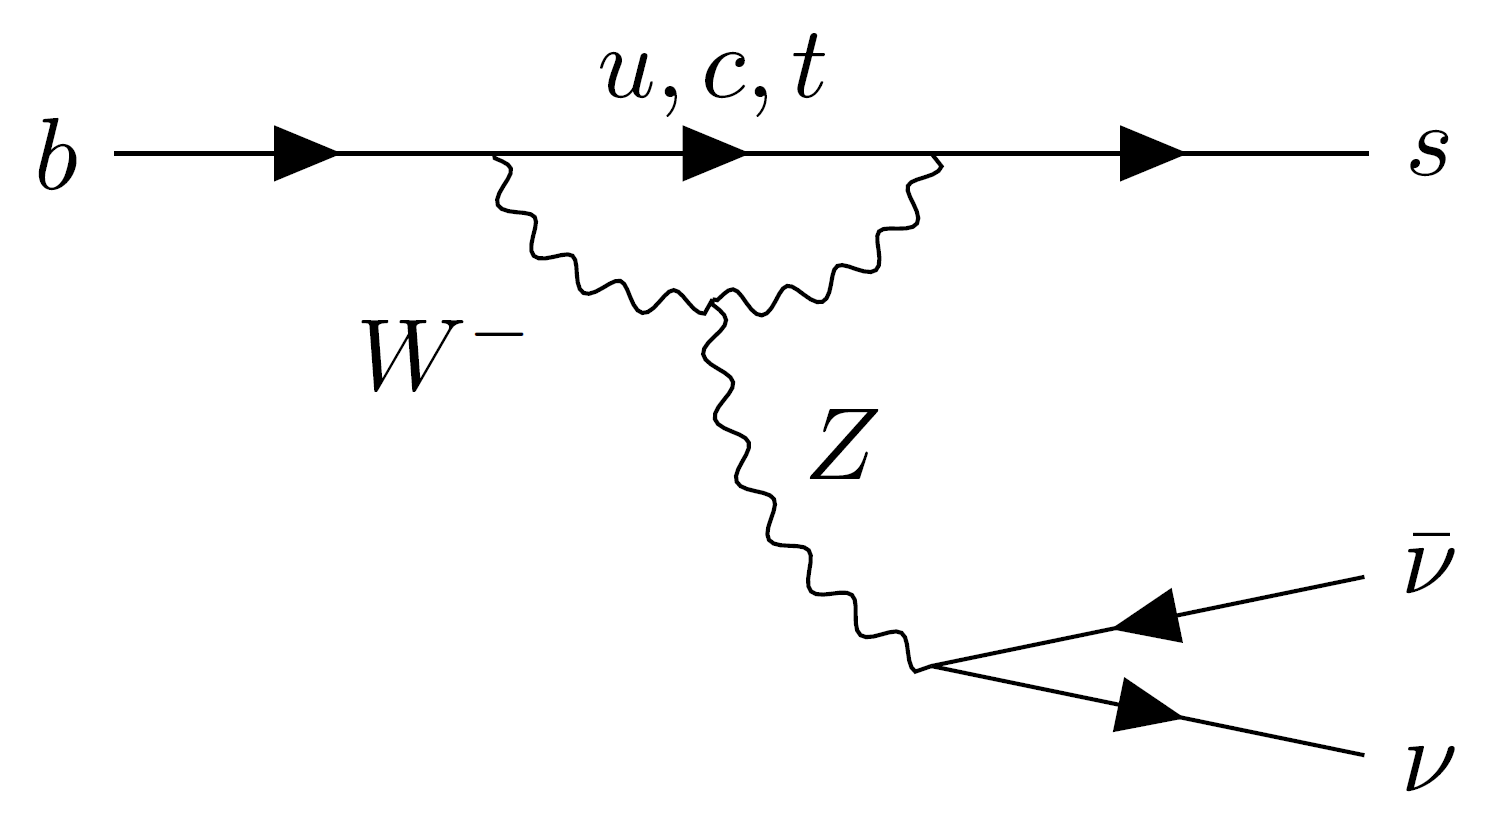
\includegraphics[width=0.4\textwidth]{./picture/EWP.png}}
    \subfloat[][box diagram]{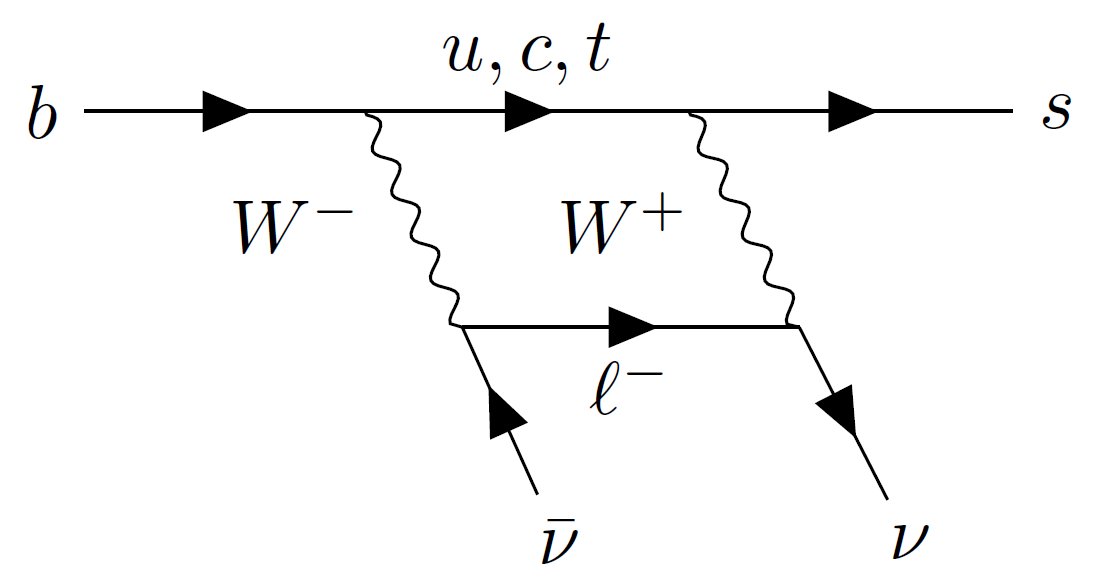
\includegraphics[width=0.4\textwidth]{./picture/BOX.png}}
    \caption{Dominant Feynman diagrams for $B\rightarrow X_{s} \nu \bar{\nu}$ decay}
    \label{fig:feynman_diagram}
\end{figure}
Since the $W$-boson and top-quark masses are much larger than the $b$-quark mass, their effects at the energy scale of $B$-meson decays can be described by local interactions among the lighter particles.
The strengths of these interactions are specified by Wilson coefficients.
The dominant Standard Model~(SM) contribution comes from diagrams involving a top quark and is proportional to $V_{tb}V_{ts}^{*}$, where $V_{ij}$ are elements of the Cabibbo--Kobayashi--Maskawa~(CKM) matrix.
The $b\rightarrow s \nu \bar{\nu}$ transition is therefore described by the following effective Hamiltonian~\cite{Altmannshofer:2009ma}:
\begin{align}
    \label{eq:hamiltonian}
    \mathcal{H}_{\textrm{eff}}=-\frac{4G_{F}}{\sqrt{2}}V_{tb}V^{*}_{ts}(C_{L}^{\nu}\mathcal{O}_{L}^{\nu}+C_{R}^{\nu}\mathcal{O}_{R}^{\nu}) + \textrm{h.c.},
\end{align}
where $C^{\nu}_{L,R}$ are the Wilson coefficients, and $\mathcal{O}_{L,R}^{\nu}$ are the operators defined as follows~\cite{Altmannshofer:2009ma}:
\begin{align}
    \label{eq:operator}
    \mathcal{O}_{L}^{\nu} = \frac{e^{2}}{16\pi^{2}}(\bar{s}\gamma_{\mu}P_{L}b)(\bar{\nu}\gamma^{\mu}(1-\gamma_{5})\nu),\quad 
\mathcal{O}_{R}^{\nu} = \frac{e^{2}}{16\pi^{2}}(\bar{s}\gamma_{\mu}P_{R}b)(\bar{\nu}\gamma^{\mu}(1-\gamma_{5})\nu).
\end{align}
In the SM, the weak interaction couples only to left-handed fermions. Therefore,
\begin{align}
    C_{R}^{\nu} = 0
\end{align}
in the SM, the effective Hamiltonian reduces to
\begin{align}
    \label{eq:hamiltonian_SM}
    \mathcal{H}_{\textrm{eff}}=-\frac{4G_{F}}{\sqrt{2}}V_{tb}V^{*}_{ts}C_{L}^{\nu}\mathcal{O}_{L}^{\nu} + \textrm{h.c.}.
\end{align}
\subsection{$B\rightarrow K\nu\bar{\nu}$}
From Eq.~\ref{eq:hamiltonian_SM}, the decay amplitude for $B\rightarrow K\nu\bar{\nu}$ can be written as follows~\cite{Ali:1999mm}:
\begin{align}
    \label{eq:Kamp}
    \mathcal{M}(b\rightarrow s \nu \bar{\nu}) \propto f_{+}(s) \left\{ (p_{B}+p)_{\mu} - \frac{m^{2}_{B}-m^{2}_{K}}{s}q_{\mu} \right\} \left( \bar{\nu} \gamma^{\mu}(1-\gamma_{5})\nu \right),
\end{align}
where $q = p_{\nu} + p_{\bar{\nu}}$ and $s = q^{2}$.
The form factor $f_{+}$ can be parametrized using the $z$ expansion~\cite{Parrott:2022rgu,Buras:2014fpa}:
\begin{align}
    \label{eq:Knunu_formfactor}
    f_{+}(q^{2})=\frac{1}{1-q^{2}/m^{2}_{+}}\left[\alpha_{0} + \alpha_{1}z(q^{2}) + \alpha_{2} z^{2}(q^{2}) + \frac{z^{3}(q^{2})}{3}(-\alpha_{1} + 2\alpha_{2}) \right],
\end{align}
where 
\begin{align}
    z(t) = \frac{\sqrt{t_{+}-t} - \sqrt{t_{+}-t_{0}}}{\sqrt{t_{+}-t} + \sqrt{t_{+}-t_{0}}},
\end{align}
with $t_{\pm}=(m_{B}\pm m_{K})^{2}$ and $t_{0}=t_{+}(1-\sqrt{1-t_{-}/t_{+}})$.

\subsection{$B\rightarrow K^{*}\nu\bar{\nu}$}
From Eq.~\ref{eq:hamiltonian_SM}, the decay amplitude for $B\rightarrow K^{*}\nu\bar{\nu}$ can be written as follows~\cite{Ali:1999mm, Biancofiore:2014uba}:
\begin{align}
    \mathcal{M}(b\rightarrow s \nu \bar{\nu}) \propto \mathcal{T}_{\mu} \left( \bar{\nu} \gamma^{\mu}(1-\gamma_{5})\nu \right),
\end{align}
where
\begin{align}
    \label{eq:Kstaramp}
    \mathcal{T}_{\mu} = (m_B+m_{K^{*}})A_{1}(s)\epsilon^{*}_{\mu}-A_{2}(q^{2})\frac{\epsilon^{*} \cdot q}{m_{B}+m_{K^{*}}}(p+p_{K^{*}})_{\mu}+i\frac{2V(s)}{m_{B}+m_{K^{*}}}\epsilon_{\mu\nu\rho\sigma}\epsilon^{*\nu}p^{\rho}p^{\sigma}_{K^{*}},
\end{align}
with three form factors $A_{1}$, $A_{2}$, and $V$.
To parametrize their $q^{2}$ dependence, we use the $z$ expansion~\cite{Bharucha:2015bzk}.
In this parametrization, $A_{12}$ is used instead of $A_{2}$.
The relation expressing $A_{2}$ in terms of $A_{1}$ and $A_{12}$ is given below.
The parametrization is written as follows:
\begin{align}
    \label{eq:Kstarnunu_formfactor}
    F(q^{2}) = \frac{q}{1-q^{2}/m^{2}_{R,F}}\left[\alpha_{0}^{F} + \alpha_{1}^{F}(z-z_{0}) + \alpha_{2}^{F}(z-z_{0})^{2} \right],
\end{align}
where $F$ denotes $A_{1}$, $A_{12}$, or $V$. Here,
\begin{align}
    A_{2} = \left[(m_{B}+m_{K^{*}})^{2}(m_{B}^{2}-m_{K^{*}}^{2}-q^{2})A_{1}-16m_{B}m_{K^{*}}(m_{B}+m_{K^{*}})A_{12} \right]/\lambda(q^{2}),
\end{align}
where
\begin{align}
    \lambda(q^{2})=m_{B}^{4}\lambda(1,m^{2}_{K^{*}}/m^{2}_{B},q^{2}/m^{2}_{B}),
    %\lambda(q^{2})=(t_{+}-q^{2})(t_{-}-q^{2}).
\end{align}
with the Källén function $\lambda(x,y,z) = x^{2} + y^{2} + z^{2} - 2xy -2yz -2zx$.
\subsection{$B\rightarrow X_{s}\nu\bar{\nu}$}
For the inclusive $B\rightarrow X_{s} \nu \bar{\nu}$ decay, the branching ratio can be written as follows~\cite{Altmannshofer:2009ma}:
\begin{align}
  \frac{d\Gamma}{dq^{2}} \propto \sqrt{\lambda(1,\hat{m}^2_s,s_b)}\left[3s_{b}(1+\hat{m}^{2}_{s}-s_{b}-4\hat{m}_{s})+\lambda(1,\hat{m}_{s}^{2},s_{b}) \right],
  \label{eq:Xsamp}
\end{align}
where $\hat{m}_s=m_{s}/m_{b}$ and $s_{b}=q^{2}/m_{b}^{2}$.

\section{Theory beyond the Standard Model}
In 2024, the Belle II collaboration reported the first evidence for the exclusive decay $B^{+}\rightarrow K^{+}\nu\bar{\nu}$, with a branching ratio of $(2.3\pm0.7)\times10^{-5}$~\cite{Belle-II:2023esi}.
The measured branching ratio is 2.7 standard deviations above the SM prediction quoted in that study.
This difference motivates further measurements of $b\rightarrow s\nu\bar{\nu}$ transitions to search for new physics.

Searches for other exclusive decays also constrain possible enhancements of $b\rightarrow s\nu\bar{\nu}$ decay rates.
The Belle collaboration set upper limits on the branching ratios of $UL(B^{0}\rightarrow K^{*0}\nu\bar{\nu})=1.8\times10^{-5}$~\cite{Belle:2017oht} and $UL(B^{+}\rightarrow K^{*+}\nu\bar{\nu})=4.0\times10^{-5}$~\cite{Belle:2013tnz}, both at the 90\% confidence level.

Models containing a $Z'$ boson~\cite{Altmannshofer:2009ma} or leptoquarks~\cite{Sahoo:2016pet} can enhance the $b\rightarrow s\nu\bar{\nu}$ decay rate.
Another possibility is the production of new invisible particles, which can give the same visible final-state particles as $b\rightarrow s\nu\bar{\nu}$~\cite{Calcuttawala:2017usw}.
In this thesis, we consider two examples illustrating these possibilities.
The first is a $Z'$ boson with flavour-changing couplings to $b$ and $s$ quarks and couplings to neutrinos, which modifies the Wilson coefficients of $b\rightarrow s\nu\bar{\nu}$~\cite{Altmannshofer:2009ma}.
The second is a light invisible scalar $S$ produced in pairs through $b\rightarrow sSS$~\cite{Calcuttawala:2017usw}.

\subsection{Flavour Violating $\bar{b}sZ'$ Coupling}
\label{sec:Zprime_model}
If there is flavour violating $\bar{b}sZ'$ coupling, the effective Lagrangian for the $b\rightarrow s \nu \bar{\nu}$ transition can be written as~\cite{Altmannshofer:2009ma}:
\begin{align}
  \mathcal{L}_{\textrm{eff}}^{\bar{b}sZ'} = \frac{G_{F}}{\sqrt{2}}\frac{e}{\pi^{2}}m^{2}_{Z'}\textrm{cos}\theta_{w}\textrm{sin}\theta_{w} V_{tb}^{*}V_{ts}Z'^{\mu}(Z'_{L}\bar{b}\gamma_{\mu}P_{L}s+Z'_{R}\bar{b}\gamma_{\mu}P_{R}s),
\end{align}
and then the Wilson coefficients in Eq.~\ref{eq:hamiltonian} become~\cite{Altmannshofer:2009ma}:
\begin{equation}
  \begin{aligned}
    \label{eq:Zprime_wilson_Xsnunubar}
    C_{L}^{\nu} = \left(C_{L}^{\nu} \right)^{\textrm{SM}} - \frac{{g'}_{V}^{\nu}}{2}Z'_{L},\\
    C_{R}^{\nu} = - \frac{{g'}_{V}^{\nu}}{2}Z'_{R}.
  \end{aligned}
\end{equation}
On the other hand, the Wilson coefficients affecting $b\rightarrow s \ell^{+} \ell^{-}$ become~\cite{Altmannshofer:2009ma}:
\begin{equation}
  \begin{aligned}
    \label{eq:Zprime_wilson_Xsellell}
    C_{10} = C_{10}^{\textrm{SM}} + \frac{{g'}_{A}^{\ell}}{2}Z'_{L},\\
    C'_{10} = +\frac{{g'}_{A}^{\ell}}{2}Z'_{R},\\
    C_{9} = C_{9}^{\textrm{SM}} - \frac{{g'}_{V}^{\ell}}{2}Z'_{L},\\
    C'_{9} = -\frac{{g'}_{V}^{\ell}}{2}Z'_{R}.
  \end{aligned}
\end{equation}
As seen in Eq.~\ref{eq:Zprime_wilson_Xsnunubar} and \ref{eq:Zprime_wilson_Xsellell}, the Wilson coefficients for $b\rightarrow s \nu \bar{\nu}$ and $b\rightarrow s \ell^{+} \ell^{-}$ are affected by different $g'$ couplings.
Therefore, in this model, the branching ratio for $B\rightarrow X_{s} \nu \bar{\nu}$ can be enhanced, while suppressing new-physics contributions to $B\rightarrow X_{s} \ell^{+} \ell^{-}$ decay.
Consequently, $B\rightarrow X_{s} \nu \bar{\nu}$ can probe new-physics models that remain unconstrained even by precise measurements of the similar FCNC process, $B\rightarrow X_{s} \ell^{+} \ell^{-}$.

\subsection{Invisible Light Scalar}
\label{sec:invisible_scalar}
For the invisible light scalar, $S$, the $b\rightarrow s SS$ transition produces the same visible final-state particles as the $b \rightarrow s \nu \bar{\nu}$ transition.
For the $b\rightarrow s SS$ transition, the effective Lagrangian can be written as follows~\cite{Calcuttawala:2017usw}:
\begin{align}
  \label{eq:lagrangian_light_scalar}
  \mathcal{L}_{\textrm{eff}}^{b\rightarrow s S S} = \frac{1}{\Lambda^{2}}\left[C_{S_{1}}m_{b}\bar{s}_{L}b_{R}S^{2}+C_{S_{2}}m_{b}\bar{b}_{L}s_{R}S^{2} + \textrm{h.c.} \right],
\end{align}
where $C_{S_{1}}$ and $C_{S_{2}}$ are Wilson coefficients.
Consequently, the search for the $B\rightarrow X_{s} \nu \bar{\nu}$ decay can constrain $C_{S_{1}}$ and $C_{S_{2}}$.
Additionally, an observed excess in the $B\rightarrow X_{s} \nu \bar{\nu}$ decay rate could provide evidence for an invisible light scalar. 

\chapter{Belle II Experiment}
In the Belle II experiment, the $e^{+}e^{-}$ beams are accelerated by SuperKEKB, and collision events are detected by the Belle II detector.
The center-of-mass energy of the Belle II experiment is mainly set to $10.58~\textrm{GeV}$, corresponding to the $\Upsilon(4S)$ resonance.
Data at energies below and above the $\Upsilon(4S)$ resonance are also collected.
Because $e^{+}e^{-}\rightarrow q\bar{q}$, where $q$ denotes a $u,d,s$, or $c$ quark, and $e^{+}e^{-}\rightarrow \tau^{+}\tau^{-}$ processes also occur at this center-of-mass energy, we can study not only $B$ physics, but also charm physics and tau physics.

\section{SuperKEKB}
This section summarizes the SuperKEKB accelerator based primarily on
the SuperKEKB Design Report~\cite{SuperKEKB:TDR}.
Figure~\ref{fig:superKEKB} shows the schematic overview of the SuperKEKB accelerator~\cite{KEK:SuperKEKBOverview}.
\begin{figure}[h]
    \centering
    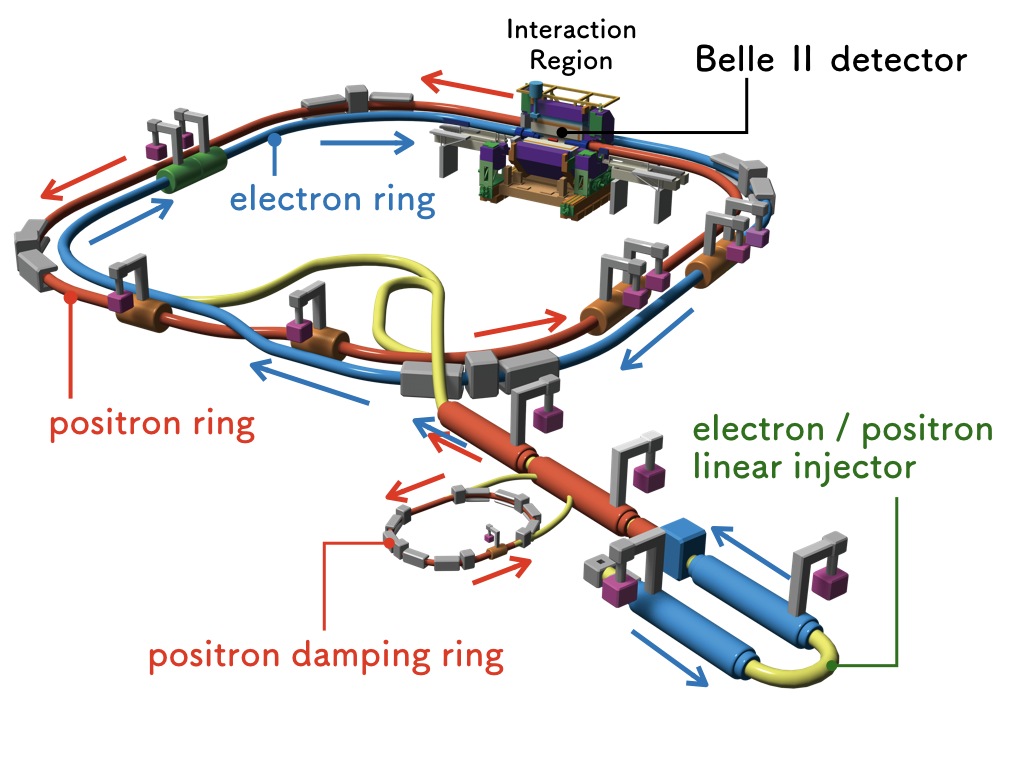
\includegraphics[width=0.7\textwidth]{./picture/superKEKB.png}
    \caption{Schematic overview of the SuperKEKB accelerator.}
    \label{fig:superKEKB}
\end{figure}
The SuperKEKB main ring consists of the High Energy Ring (HER) and the Low
Energy Ring (LER).
In the HER and LER, $7~\textrm{GeV}$ electron beams and $4~\textrm{GeV}$ positron beams circulate, respectively.
For the electron beam in the HER, a photo-cathode RF gun is used to obtain low-emittance and high-current electrons.
For the positron beams in the LER, high-current primary electrons are first produced by a thermionic gun.
Then positrons are obtained by making these primary electrons collide with a tungsten target.
Electrons and positrons are accelerated to $7~\textrm{GeV}$ and $4~\textrm{GeV}$, respectively, then injected into the main ring.

In the accelerator description, $x$ and $y$ denote the horizontal and vertical directions transverse to the reference beam trajectory, respectively.
For flat beams, whose horizontal size is much larger than their vertical size, the luminosity $\mathcal{L}$ is given by the following proportionality~\cite{Zhou_2024}:
\begin{equation}
  \label{eq:lumi}
  \mathcal{L} \propto \frac{I_{+}I_{-}}{\beta^{*}_{y+}\beta^{*}_{y-}},
\end{equation}
where $I$ is the beam currents, $\beta^{*}_{y}$ is the vertical beta function at the interaction point~(IP), and the subscripts $+$ and $-$ denote the $e^{+}$ and $e^{-}$ beams, respectively.
To achieve higher luminosity, the KEKB accelerator, the predecessor of SuperKEKB, was upgraded.
Table~\ref{tab:accelerator_params} shows the parameter values and luminosity for KEKB and SuperKEKB accelerator~\cite{Zhou_2024,Natochii:2023thp}.
\begin{table}
\caption{Comparison of parameters and luminosity between KEKB and SuperKEKB accelerators}
    \centering
    \begin{tabular}{ p{3cm} p{5cm} p{5cm} p{5cm} p{5cm}  }
    \hline
    \multicolumn{1}{c}{} &  \multicolumn{2}{c}{KEKB} & \multicolumn{2}{c}{SuperKEKB} \\
    \multicolumn{1}{c}{} &  \multicolumn{2}{c}{Achieved} & \multicolumn{2}{c}{Target} \\
    \hline
    \multicolumn{1}{c}{} &  \multicolumn{1}{c}{LER} & \multicolumn{1}{c}{HER} & \multicolumn{1}{c}{LER} & \multicolumn{1}{c}{HER} \\
    \hline
    \multicolumn{1}{c}{$I_{\textrm{beam}}$ [A]} & \multicolumn{1}{c}{1.637} & \multicolumn{1}{c}{1.188} & \multicolumn{1}{c}{2.80} & \multicolumn{1}{c}{2.00} \\
    \multicolumn{1}{c}{$\beta^{*}_{y}$ [mm]} & \multicolumn{1}{c}{5.9} & \multicolumn{1}{c}{5.9} & \multicolumn{1}{c}{0.27} & \multicolumn{1}{c}{0.3} \\
    \multicolumn{1}{c}{$\mathcal{L}$ [$10^{34}~\textrm{cm}^{-2}\textrm{s}^{-1}$]} & \multicolumn{2}{c}{2.11} & \multicolumn{2}{c}{60} \\
    \multicolumn{1}{c}{$\int \mathcal{L} dt$ [$\textrm{ab}^{-1}$]} & \multicolumn{2}{c}{1.04} & \multicolumn{2}{c}{50} \\
  \hline
\end{tabular}
    \label{tab:accelerator_params}
\end{table}
As seen in Eq.~\ref{eq:lumi} and Table~\ref{tab:accelerator_params}, the beam currents are increased to achieve higher luminosity during the upgrade from KEKB to SuperKEKB.
According to Eq.~\ref{eq:lumi}, decreasing $\beta^{*}_{y}$ can also improve the luminosity.
However, to limit the luminosity loss due to the hourglass effect, the vertical beta function at the IP should satisfy~\cite{Ohnishi:2013fma}
\begin{equation}
  \beta^{*}_{y} \geq \ell_{\textrm{overlap}},
\end{equation}
where $\ell_{\textrm{overlap}}$ is the effective longitudinal overlap length of the two beams.
For head-on collisions, this relation becomes~\cite{SuperKEKB:TDR}
\begin{equation}
  \beta^{*}_{y} \geq \sigma_{z},
\end{equation}
where $\sigma_{z}$ is the bunch length.

SuperKEKB employs the nano-beam scheme, which combines a small horizontal beam size with a large horizontal crossing angle~\cite{Akai:2018mbz}.
In the nano-beam scheme, the overlap length is approximately given by~\cite{Akai:2018mbz}
\begin{equation}
  \ell_{\textrm{overlap}} \sim \frac{\sigma_{x}^{*}}{\theta_{x}},
\end{equation}
where $2\theta_{x}$ is the crossing angle between beams.
The horizontal beam size at the IP, $\sigma_{x}^{*}$, is given by~\cite{Holzer:2013lbc}
\begin{equation}
    \sigma_{x}^{*} \simeq \sqrt{\varepsilon_{x}\beta_{x}^{*}},
\end{equation}
where $\varepsilon_x$ is the horizontal geometric emittance, which characterizes the spread of particles in horizontal position and angle, and $\beta_{x}^{*}$ is the horizontal beta function at the IP.
Thus, the low horizontal emittance helps reduce the horizontal beam size, which, together with the large horizontal crossing angle, shortens the overlap length and allows a smaller $\beta^{*}_{y}$ while limiting the luminosity loss due to the hourglass effect.

\section{Belle II detector}
Figure~\ref{fig:BelleII} shows a schematic overview of the Belle II detector~\cite{KEK:BelleIIDetectorOverviewImage}.
The Belle II detector consists of seven sub-detectors: the Pixel Detector~(PXD), the Silicon Vertex Detector~(SVD), the Central Drift Chamber~(CDC), the Time-of-Propagation~(TOP) counter, the Aerogel Ring-Imaging Cherenkov counter~(ARICH), the Electromagnetic Calorimeter~(ECL), and the $K_{L}^{0}$ and $\mu$ detector~(KLM).
In this section, the concepts of the sub-detector systems, trigger system, and data acquisition system are discussed.
\begin{figure}[h]
    \centering
    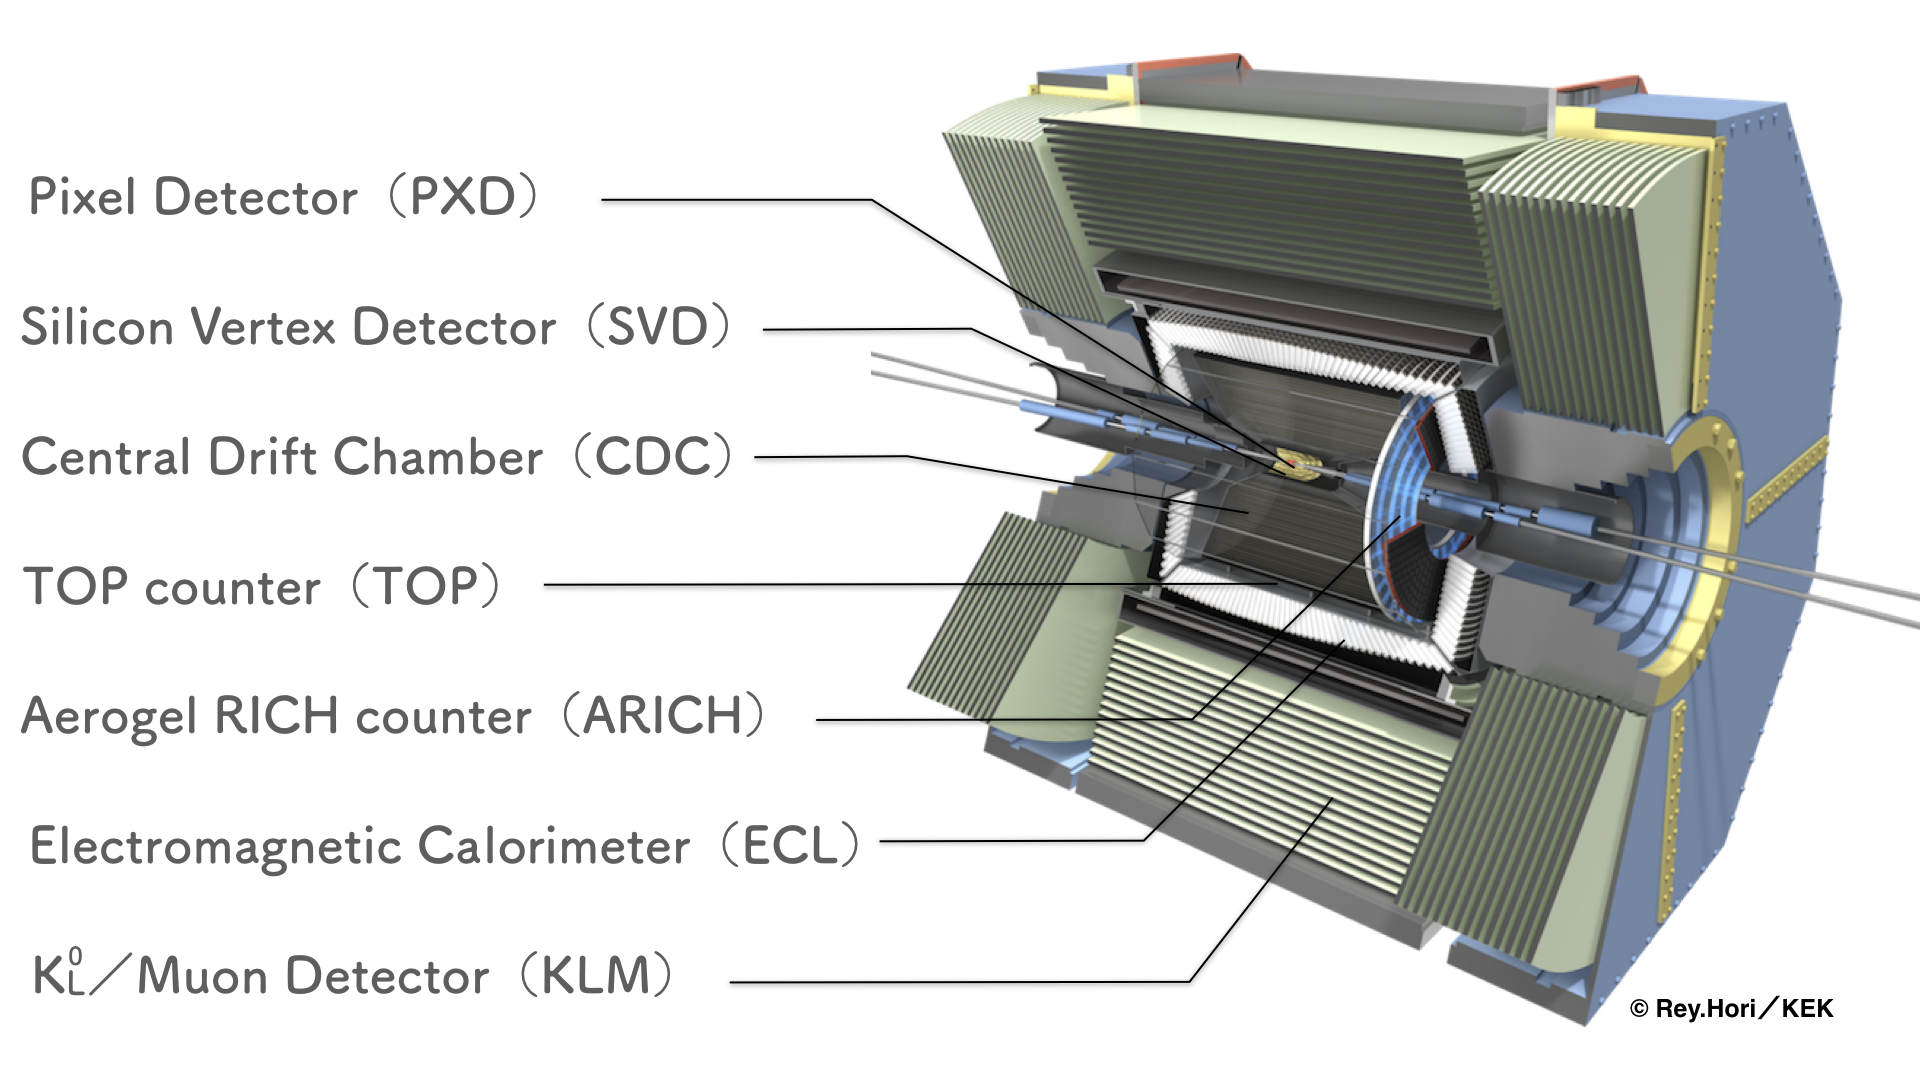
\includegraphics[width=0.8\textwidth]{./picture/BelleII.png}
    \caption{Schematic overview of the Belle II detector.}
    \label{fig:BelleII}
\end{figure}

In the Belle II experiment, a right-handed Cartesian coordinate system, $(x,y,z)$, is used.
The origin is defined as the interaction point~(IP).
The $x$-axis points horizontally outward from the center of the main ring.
The $y$-axis points vertically upward.
The $z$-axis is aligned with the direction of the solenoidal magnetic field and coincides with the bisector of the LER and HER beams.
The azimuthal angle $\phi$ is defined by $\sin\phi = y/\sqrt{x^2+y^2}$ and $\cos\phi = x/\sqrt{x^2+y^2}$.
The polar angle $\theta$ is defined by $\sin\theta = \sqrt{x^2+y^2}/\sqrt{x^2+y^2+z^2}$ and $\cos\theta = z/\sqrt{x^2+y^2+z^2}$.

\subsection{Pixel Detector (PXD)}
Figure~\ref{fig:PXD} shows a schematic overview of the PXD~\cite{Belle-II:2010dht}.
The PXD consists of two layers.
In each layer, PXD modules are arranged in a windmill structure~\cite{Belle-IIDEPFET:2022wis}.
The inner layer has a radius of 14~mm and consists of 8 planar modules.
The outer layer has a radius of 22~mm and consists of 12 planar modules.
\begin{figure}[h]
    \centering
    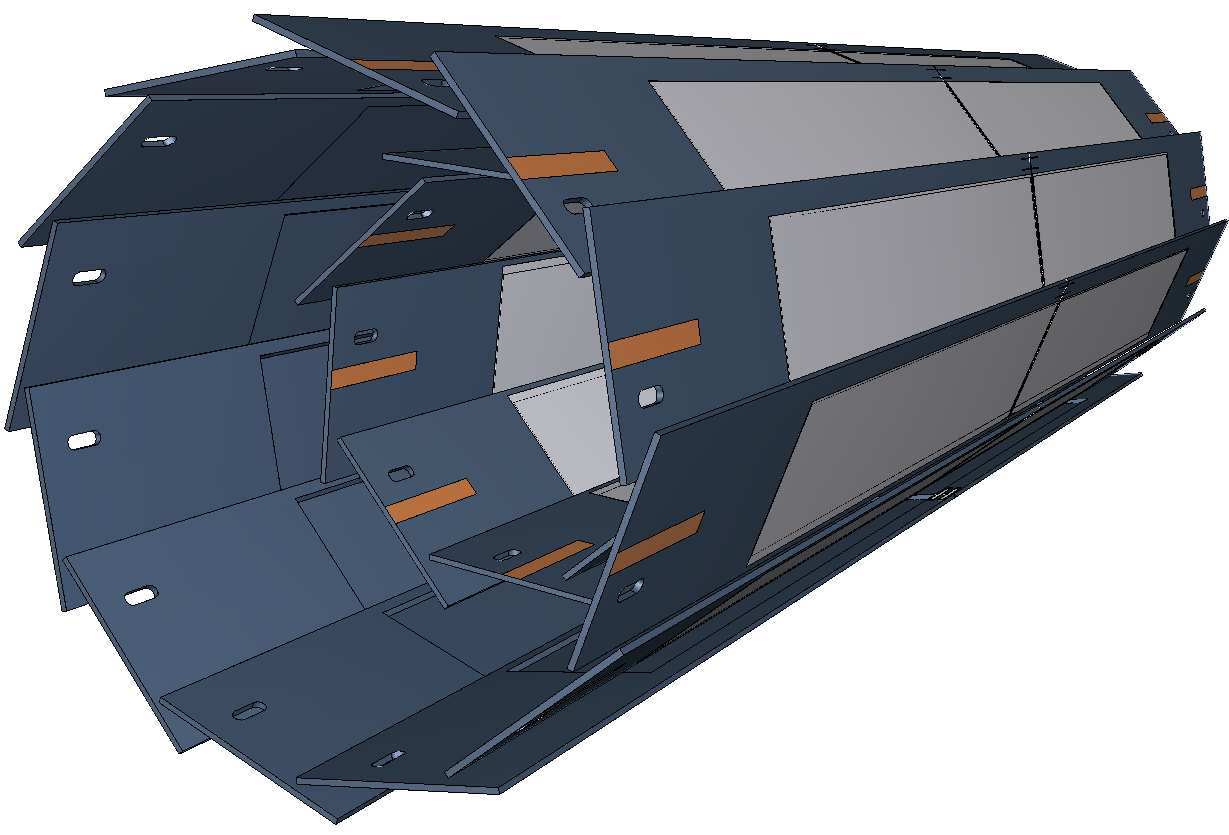
\includegraphics[width=0.65\textwidth]{./picture/PXD.png}
    \caption{Schematic overview of the PXD.}
    \label{fig:PXD}
\end{figure}

The PXD sensor uses the DEPleted Field Effect Transistor~(DEPFET) technology~\cite{Kemmer:1986vh}.
While the readout ASICs at the module ends require a CO$_2$ cooling system, the low power consumption of the DEPFET sensor allows its active area to be cooled by a flow of nitrogen gas~\cite{Belle-II:2010dht,BelleIIPXD:2020ete}.
Additionally, the internal signal amplification and low noise of DEPFET sensors allow sufficient signal-to-noise ratios even in thin active regions~\cite{Schwenker:2017kcf}.
In the Belle II PXD, the active region of each DEPFET sensor is thinned to $75~\mu\textrm{m}$, reducing the sensor contribution to the material budget.
Each PXD module consists of $250 \times 768$ DEPFET pixel sensors.

The resolution in the $xy$ plane is $13.64\pm0.11~\mu\textrm{m}$.
The resolution along the $z$-axis is $14.92\pm0.07~\mu\textrm{m}$~\cite{Belle-IIDEPFET:2022wis}.

\subsection{Silicon Vertex Detector (SVD)}
Figure~\ref{fig:SVD} shows a schematic overview of the SVD~\cite{BelleIISVD:2019xws}.
\begin{figure}[h]
    \centering
    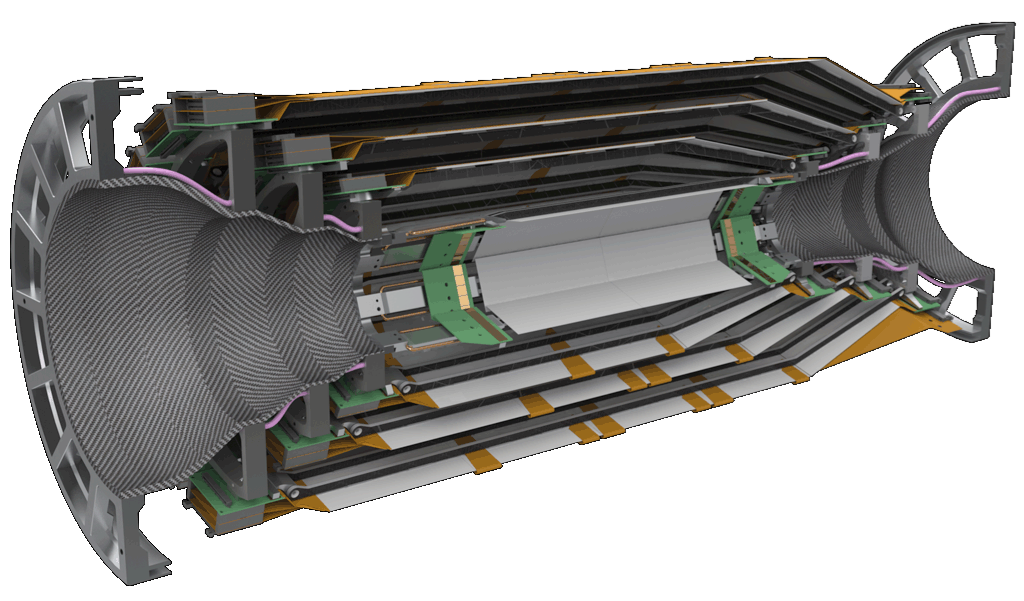
\includegraphics[width=0.65\textwidth]{./picture/SVD.png}
    \caption{Schematic overview of the SVD.}
    \label{fig:SVD}
\end{figure}
The SVD consists of four layers.
Each layer consists of ladders arranged in a windmill structure.
Each ladder comprises multiple silicon strip sensors, as summarized in Table~\ref{tab:SVD_config}~\cite{Belle-II:2010dht}.
\begin{table}
    \caption{geometrical configuration of the SVD.}
    \centering
    \begin{tabular}{ p{3cm} p{5cm} p{5cm} p{5cm} p{5cm}  }
    \hline
    \multicolumn{1}{c}{Layer} & \multicolumn{1}{c}{Radius~(mm)} & \multicolumn{1}{c}{Ladders} & \multicolumn{1}{c}{Sensors/ladder} & \multicolumn{1}{c}{Sensors} \\
    \hline
    \multicolumn{1}{c}{6} & \multicolumn{1}{c}{140} & \multicolumn{1}{c}{17} & \multicolumn{1}{c}{5} & \multicolumn{1}{c}{85} \\
    \multicolumn{1}{c}{5} & \multicolumn{1}{c}{115} & \multicolumn{1}{c}{14} & \multicolumn{1}{c}{4} & \multicolumn{1}{c}{56} \\
    \multicolumn{1}{c}{4} & \multicolumn{1}{c}{80} & \multicolumn{1}{c}{10} & \multicolumn{1}{c}{3} & \multicolumn{1}{c}{30} \\
    \multicolumn{1}{c}{3} & \multicolumn{1}{c}{38} & \multicolumn{1}{c}{8} & \multicolumn{1}{c}{2} & \multicolumn{1}{c}{16} \\
  \hline
\end{tabular}
    \label{tab:SVD_config}
\end{table}
The SVD uses double-sided silicon strip detector~(DSSD) technology.

The SVD adopts the \textit{origami} chip-on-sensor concept~\cite{Irmler:2013nc}.
In the \textit{origami} scheme, a readout chip is placed on one side of the DSSD.
The other side of the DSSD is connected to the readout chip by flexible electronic circuits.
This \textit{origami} structure requires a single cooling channel, which leads to a low material budget~\cite{BelleIISVD:2019xws}.
The average material budget of the SVD is approximately $0.7\%$ of a radiation length per layer~\cite{Belle-IISVD:2022ofq}.

The two sides of each DSSD are referred to as the P-side and N-side, according to the p-type and n-type doping of their implanted strips, respectively.
The strips on the two sides are oriented perpendicular to each other, allowing the two-dimensional position of a particle hit to be measured~\cite{BelleIISVD:2021vwi}.
The cluster position resolutions on the P-side and N-side are approximately $9~\mu\textrm{m}$ and $20~\mu\textrm{m}$, respectively, for layer 3, and $11~\mu\textrm{m}$ and $25~\mu\textrm{m}$ for layers 4--6.
The average sensor hit efficiency exceeds $99\%$~\cite{BelleIISVD:2021vwi}.

\subsection{Central Drift Chamber (CDC)}
Figure~\ref{fig:CDC} shows a schematic overview of the longitudinal cross section of the CDC~\cite{Dong:2019wtj}.
\begin{figure}[h]
    \centering
    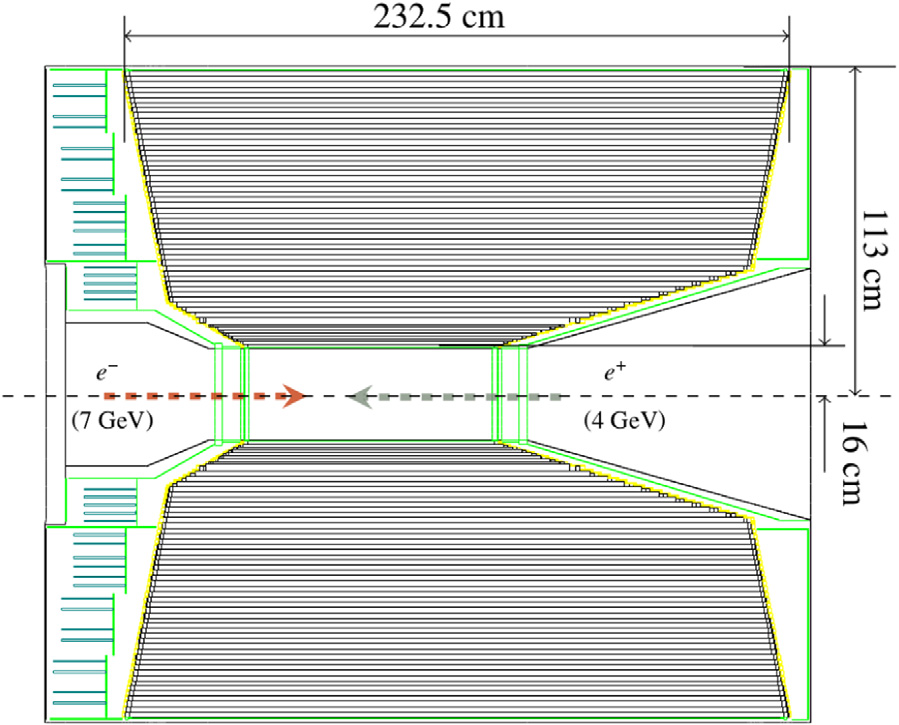
\includegraphics[width=0.55\textwidth]{./picture/CDC.png}
    \caption{Longitudinal cross section of the CDC.}
    \label{fig:CDC}
\end{figure}
A mixture of 50\% He and 50\% $\textrm{C}_{2}\textrm{H}_{6}$ is used because of its long radiation length, high drift velocity, and good energy loss resolution~\cite{Belle-II:2010dht}.

The CDC consists of 56 wire layers.
The layers can be classified into two types: axial and stereo layers.
In the axial layers, wires are parallel to the $z$-axis.
On the other hand, in the stereo layer, wires are skewed with respect to the $z$-axis.
These different types of layers are needed to determine the three-dimensional positions of tracks.
Adjacent layers of the same type are grouped into superlayers, and there are five axial superlayers and four stereo superlayers.
Figure~\ref{fig:CDC_info_plots} shows the layer layouts of the CDC in the Belle and Belle II experiments~\cite{Dong:2019wtj}, together with schematic illustrations of axial and stereo layers~\cite{frost_oliver_2013_21906}.
The U and V types of stereo wires denote the skew directions of the wires.
\begin{figure}[htbp]
    \centering
    \begin{minipage}[c]{0.58\textwidth}
        \centering
        \subfloat[\label{fig:CDC_layer}]{
            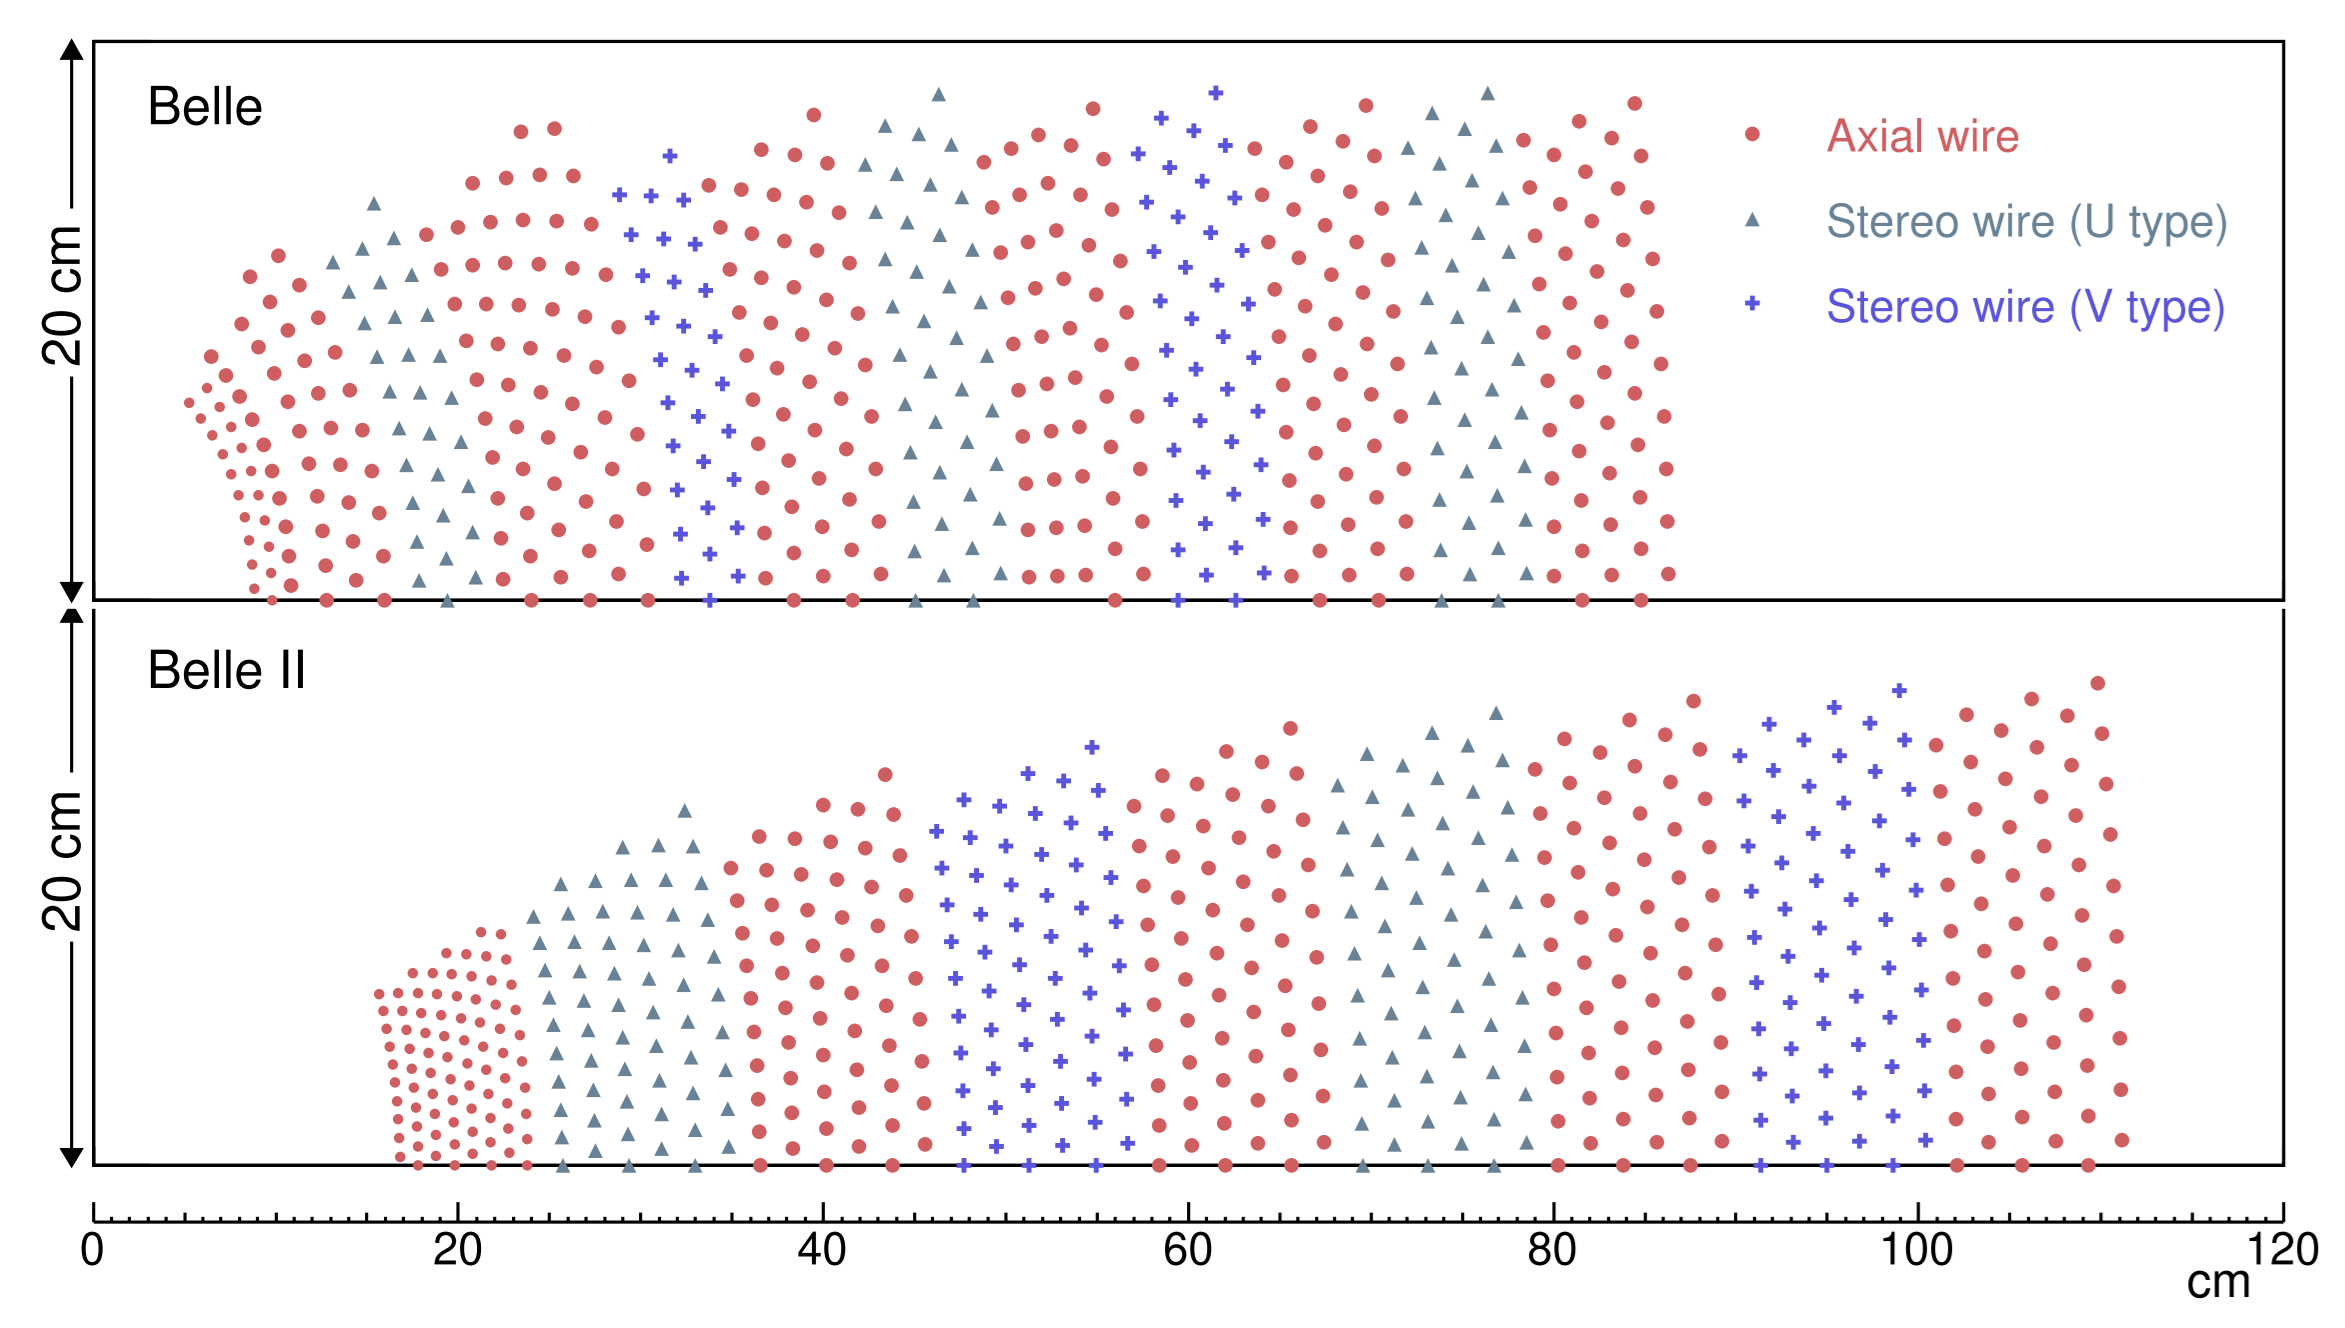
\includegraphics[width=\textwidth]{./picture/CDC_layer.png}
        }
    \end{minipage}
    \hfill
    \begin{minipage}[c]{0.38\textwidth}
        \centering
        \subfloat[\label{fig:right_top}]{
            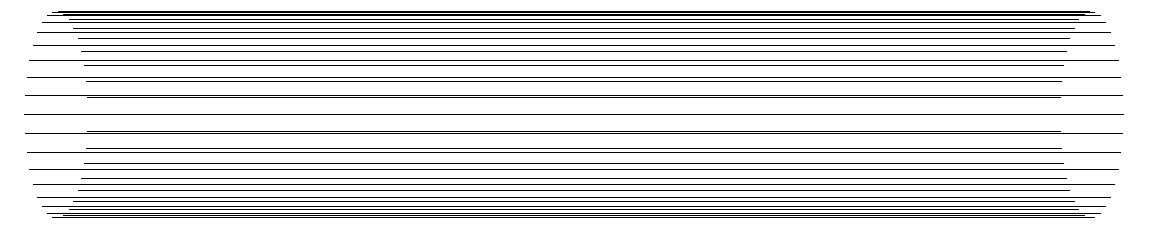
\includegraphics[width=\textwidth]{./picture/axial_wire.png}
        }
        \vspace{0.5cm}
        \subfloat[\label{fig:right_bottom}]{
            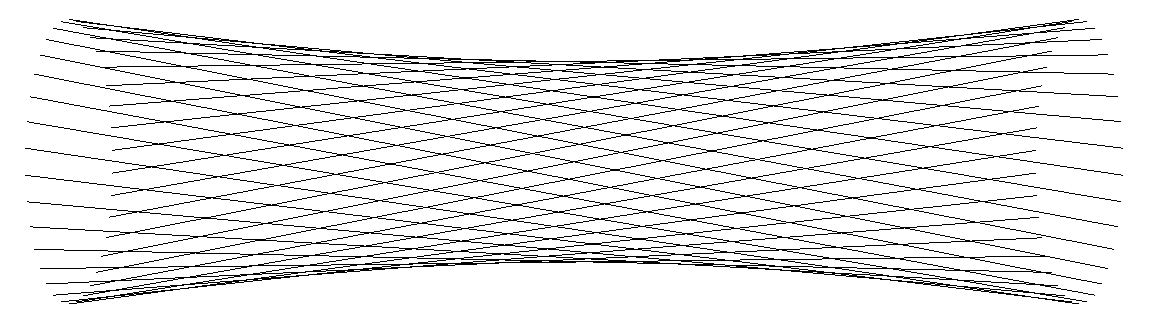
\includegraphics[width=\textwidth]{./picture/stereo_wire.png}
        }
    \end{minipage}
    \caption{(a) Layer layouts of the CDC in the Belle and Belle II experiments. The U and V types of stereo wires denote the skew directions of the wires. (b) Schematic illustration of an axial layer. (c) Schematic illustration of a stereo layer.}
    \label{fig:CDC_info_plots}
\end{figure}

The CDC achieves a position resolution better than $120~\mu\textrm{m}$, depending on the wire layer and track incidence angles~\cite{Dong:2019wtj}.
The relative transverse momentum resolution measured with cosmic-ray tracks is parametrized as~\cite{Dong:2019wtj}
\begin{equation}
    \frac{\sigma_{p_{T}}}{p_{T}}
    =
    \sqrt{\left(0.127\frac{p_{T}}{\textrm{GeV}/c}\right)^2 + 0.321^2}\%,
\end{equation}
where $p_{T}$ is the transverse momentum.

\subsection{Time-of-Propagation (TOP) counter}
The Time-of-Propagation~(TOP) detector is installed for particle identification in the barrel region of the Belle II detector.
Figure~\ref{fig:TOP} shows a schematic overview of the TOP detector and a TOP module~\cite{Atmacan:2025jmh}.
The TOP detector consists of 16 modules.
\begin{figure}[h]
    \centering
    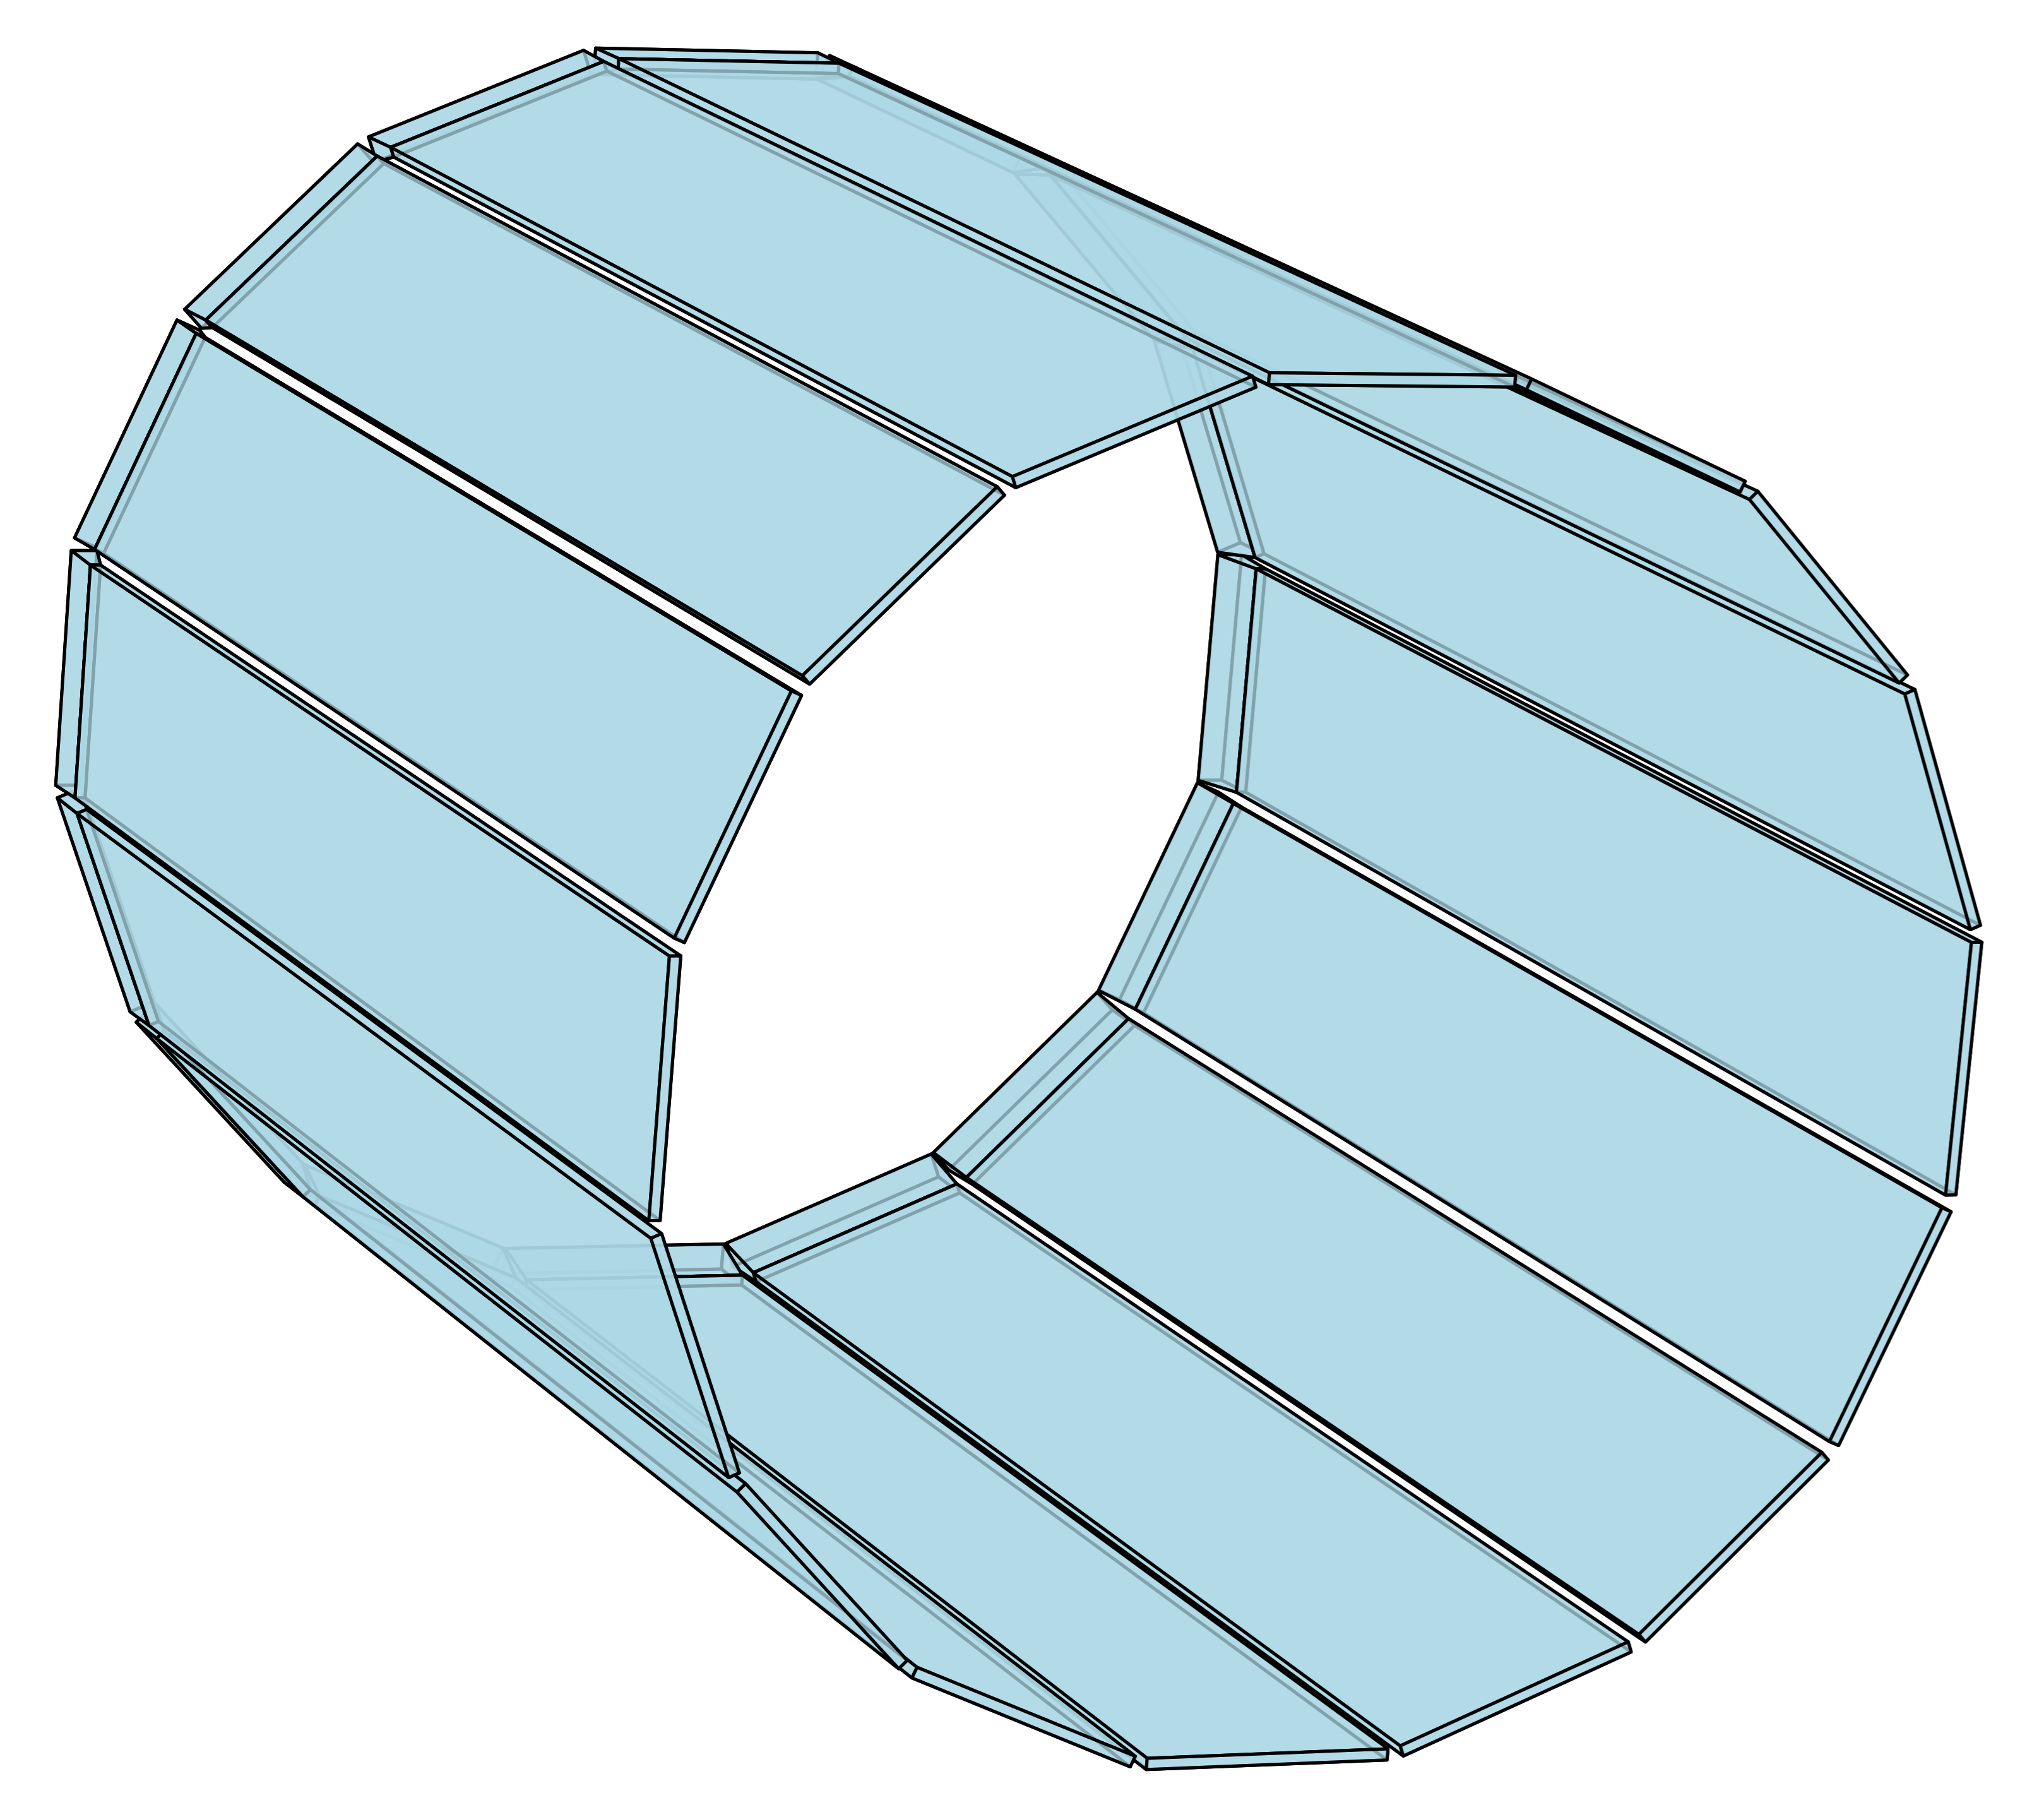
\includegraphics[width=0.48\textwidth]{./picture/TOP.png}
    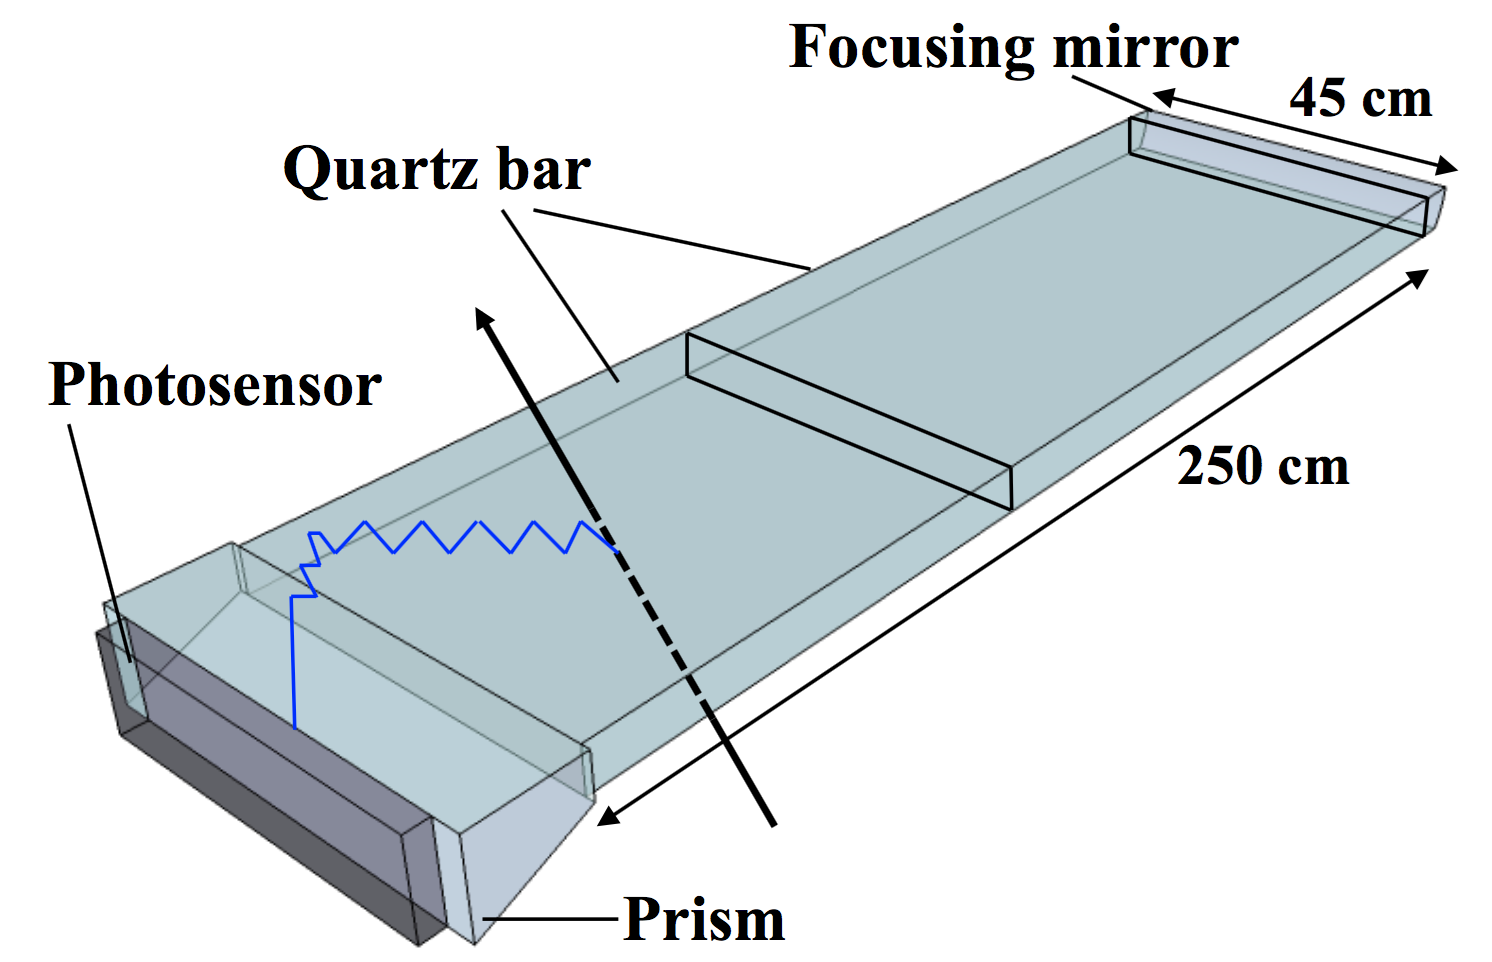
\includegraphics[width=0.48\textwidth]{./picture/TOP_module.png}
    \caption{(Left) Schematic overview of the TOP detector and (right) a TOP module.}
    \label{fig:TOP}
\end{figure}

The TOP detector uses Cherenkov radiation to identify particles.
When a particle with speed $c\beta$ passes through a material, Cherenkov radiation is emitted at an angle $\theta_c$~\cite{ParticleDataGroup:2024cfk}:
\begin{equation}
  \label{eq:cherenkov}
  \cos \theta_{c} = \frac{1}{n \beta},
\end{equation}
where $n$ is the refractive index of the material.
For the same momentum, the Cherenkov angle $\theta_{c}$ is larger for $\pi$ than for $K$.
Consequently, Cherenkov photons from $\pi$ arrive at the photon sensors earlier than those from $K$.
This difference in time of propagation enables particle identification.
Figure~\ref{fig:TOP_plot} shows a schematic overview of Cherenkov radiation for $K$ and $\pi$~\cite{Kotchetkov:2018qzw}, and simulated time-of-propagation distributions~\cite{Fast:2017pff}.
As seen in the figure, there is a difference in the time of propagation between $\pi$ and $K$.
\begin{figure}[h]
    \centering
    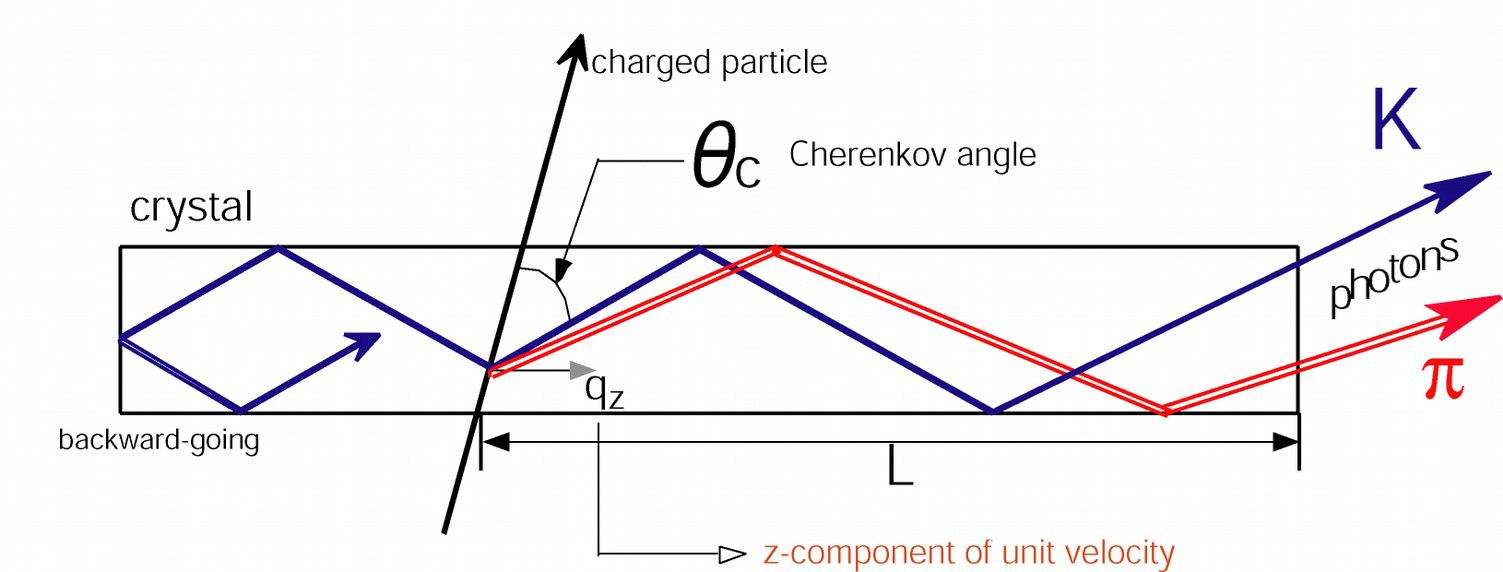
\includegraphics[width=0.48\textwidth]{./picture/TOP_cherenkov.png}
    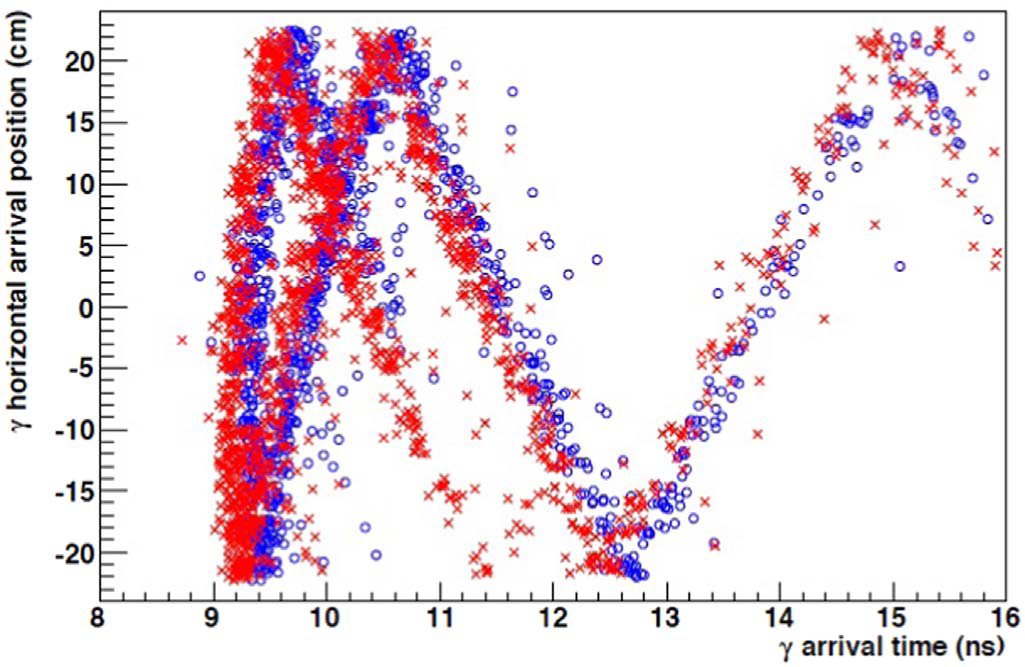
\includegraphics[width=0.48\textwidth]{./picture/TOP_distribution.png}
    \caption{(Left) Schematic overview of Cherenkov radiation for $K$ and $\pi$. (Right) Simulated distributions of Cherenkov-photon arrival time and horizontal detection position for $K$ (blue circles) and $\pi$ (red crosses).}
    \label{fig:TOP_plot}
\end{figure}

The TOP detector provides pion and kaon identification efficiencies at the $90\%$ level, with misidentification rates of approximately $10\%$, depending on the track momentum, polar angle, and likelihood-ratio selection~\cite{Atmacan:2025jmh}.

\subsection{Aerogel Ring-Imaging Cherenkov counter~(ARICH)}
For particle identification in the end-cap region, the Aerogel Ring-Imaging Cherenkov~(ARICH) detector is used.
Similar to the TOP detector, the ARICH detector uses Cherenkov radiation.
Instead of using the propagation time, the ARICH detector uses ring images of Cherenkov radiation.

In the ARICH detector, aerogel layers are used as radiators.
Two aerogel layers with average refractive indices of 1.045 and 1.055~\cite{Santelj:2023iim} are used to increase the number of detected photons without degrading the Cherenkov angle resolution~\cite{Iwata:2016flq}.
To detect photons, hybrid avalanche photo-detectors~(HAPDs) are used.
Figure~\ref{fig:ARICH_principle} shows schematic illustrations of the two aerogel layers and the ring image produced by the ARICH detector~\cite{Iwata:2016flq}.
\begin{figure}[h]
    \centering
    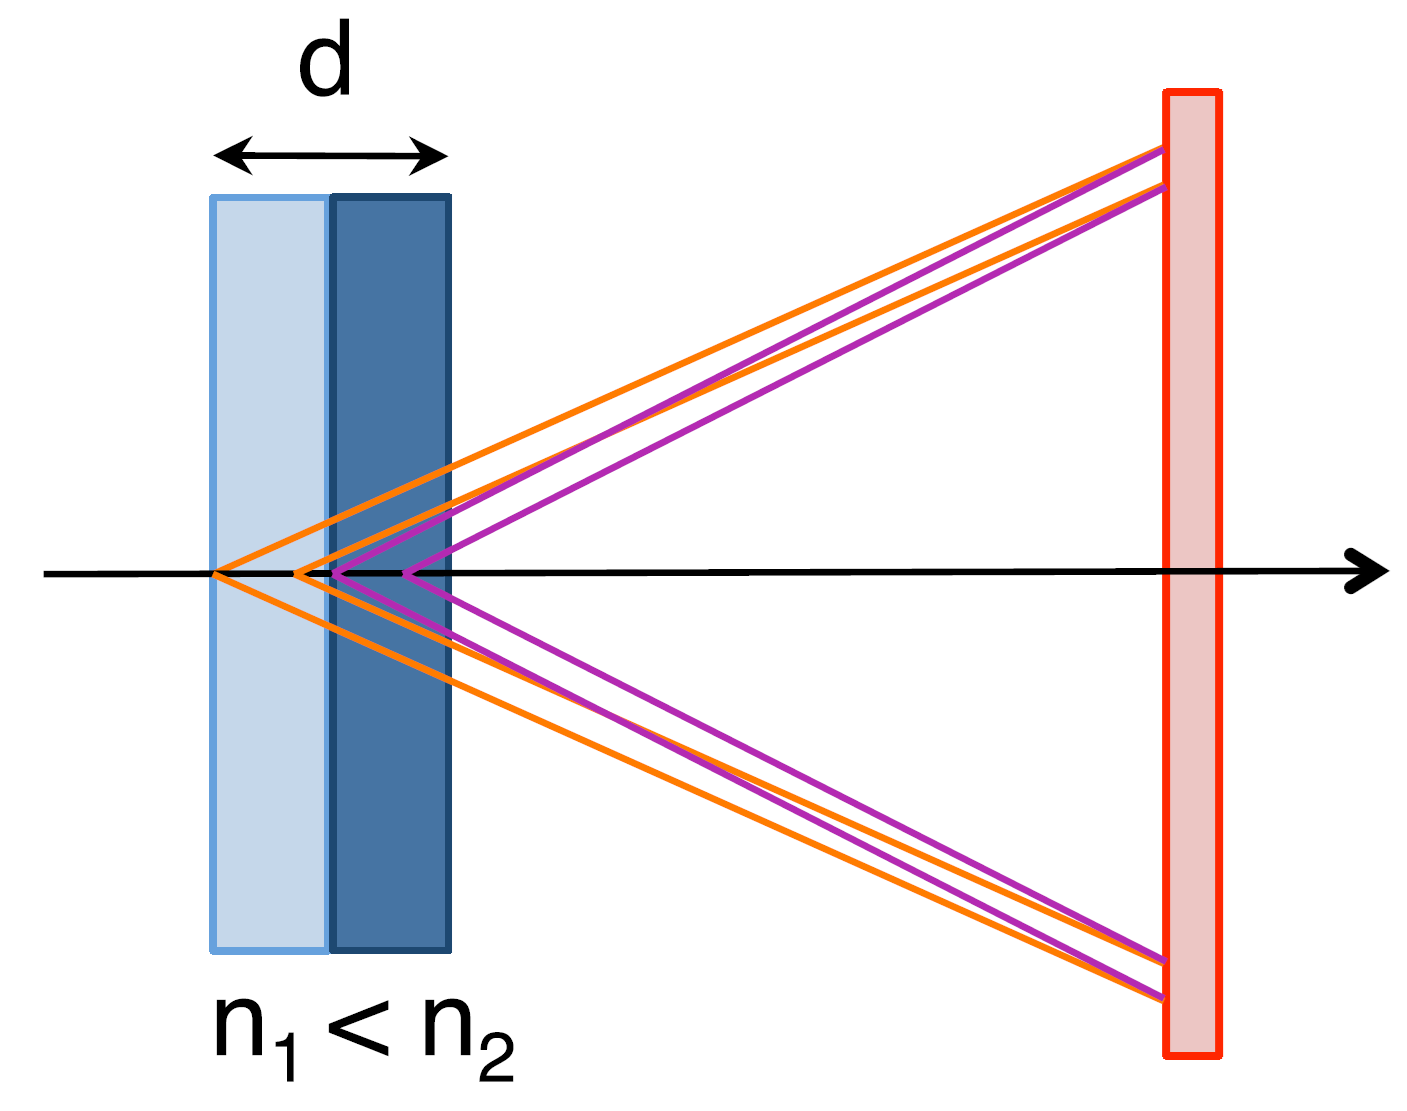
\includegraphics[width=0.45\textwidth]{./picture/ARICH_principle_2.png}
    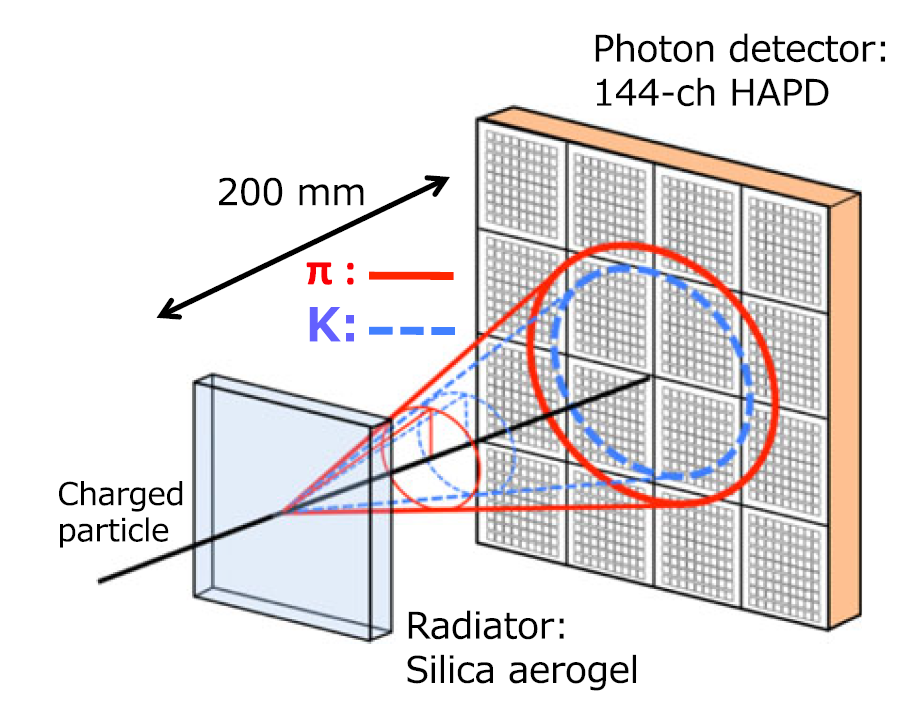
\includegraphics[width=0.45\textwidth]{./picture/ARICH_principle_1.png}
    \caption{(Left) Schematic overview of the two aerogel layers. (Right) Schematic overview of a ring image produced by the ARICH detector.}
    \label{fig:ARICH_principle}
\end{figure}
From this ring image, the Cherenkov angle can be measured directly.
Figure~\ref{fig:ARICH} shows a schematic overview of the arrangement of the photon detectors and aerogel radiators, together with the ARICH detector~\cite{Santelj:2023iim}.
\begin{figure}[h]
    \centering
    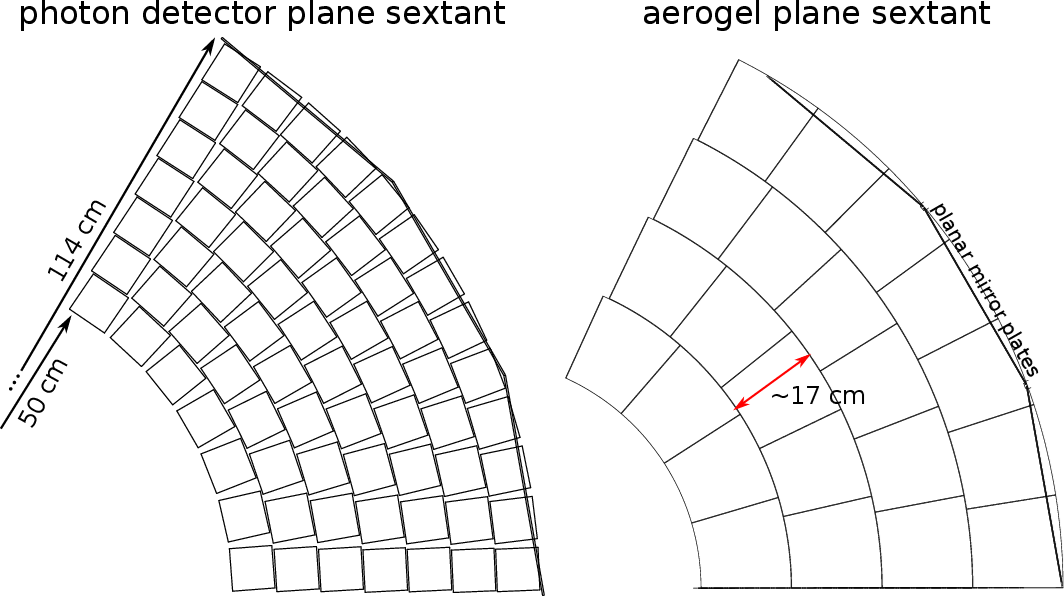
\includegraphics[width=0.55\textwidth]{./picture/ARICH_config.png}
    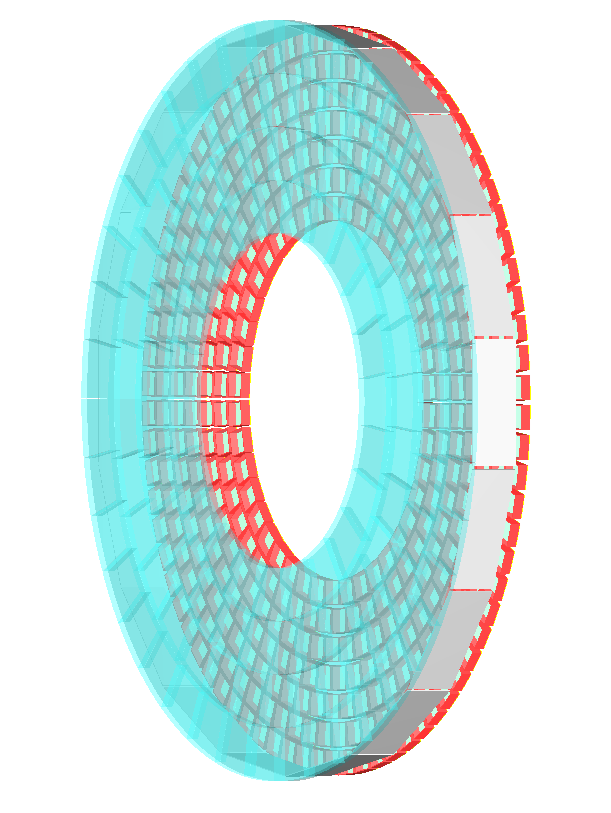
\includegraphics[width=0.25\textwidth]{./picture/ARICH.png}
    \caption{(Left) Schematic overview of the arrangement of the photon detectors and aerogel radiators. (Right) Schematic overview of the ARICH detector.}
    \label{fig:ARICH}
\end{figure}

The single-photon Cherenkov angle resolution is $12.7~\textrm{mrad}$, with an average of 11.4 detected photons per track, as measured using muons from $e^{+}e^{-}\to\mu^{+}\mu^{-}$ events~\cite{Santelj:2023iim}.
The ARICH detector achieved a kaon identification efficiency of $(93.5\pm0.6)\%$ at a pion misidentification probability of $(10.9\pm0.9)\%$~\cite{Yonenaga:2020eby}.

\subsection{Electromagnetic Calorimeter~(ECL)}
In the Belle II experiment, a homogeneous electromagnetic calorimeter is used.
The ECL consists of CsI(Tl) crystals, whose cross section is $6\times6~\textrm{cm}^{2}$ on average and whose length is 30~cm ($16.2X_{0}$)~\cite{Shebalin:2018sll}.
There are 8736 crystals in total: 1152 in the forward endcap, 960 in the backward endcap, and 6624 in the barrel region.
Figure~\ref{fig:ECL} shows a schematic overview of the ECL and a CsI(Tl) crystal~\cite{Shebalin:2018sll}.
\begin{figure}[h]
    \centering
    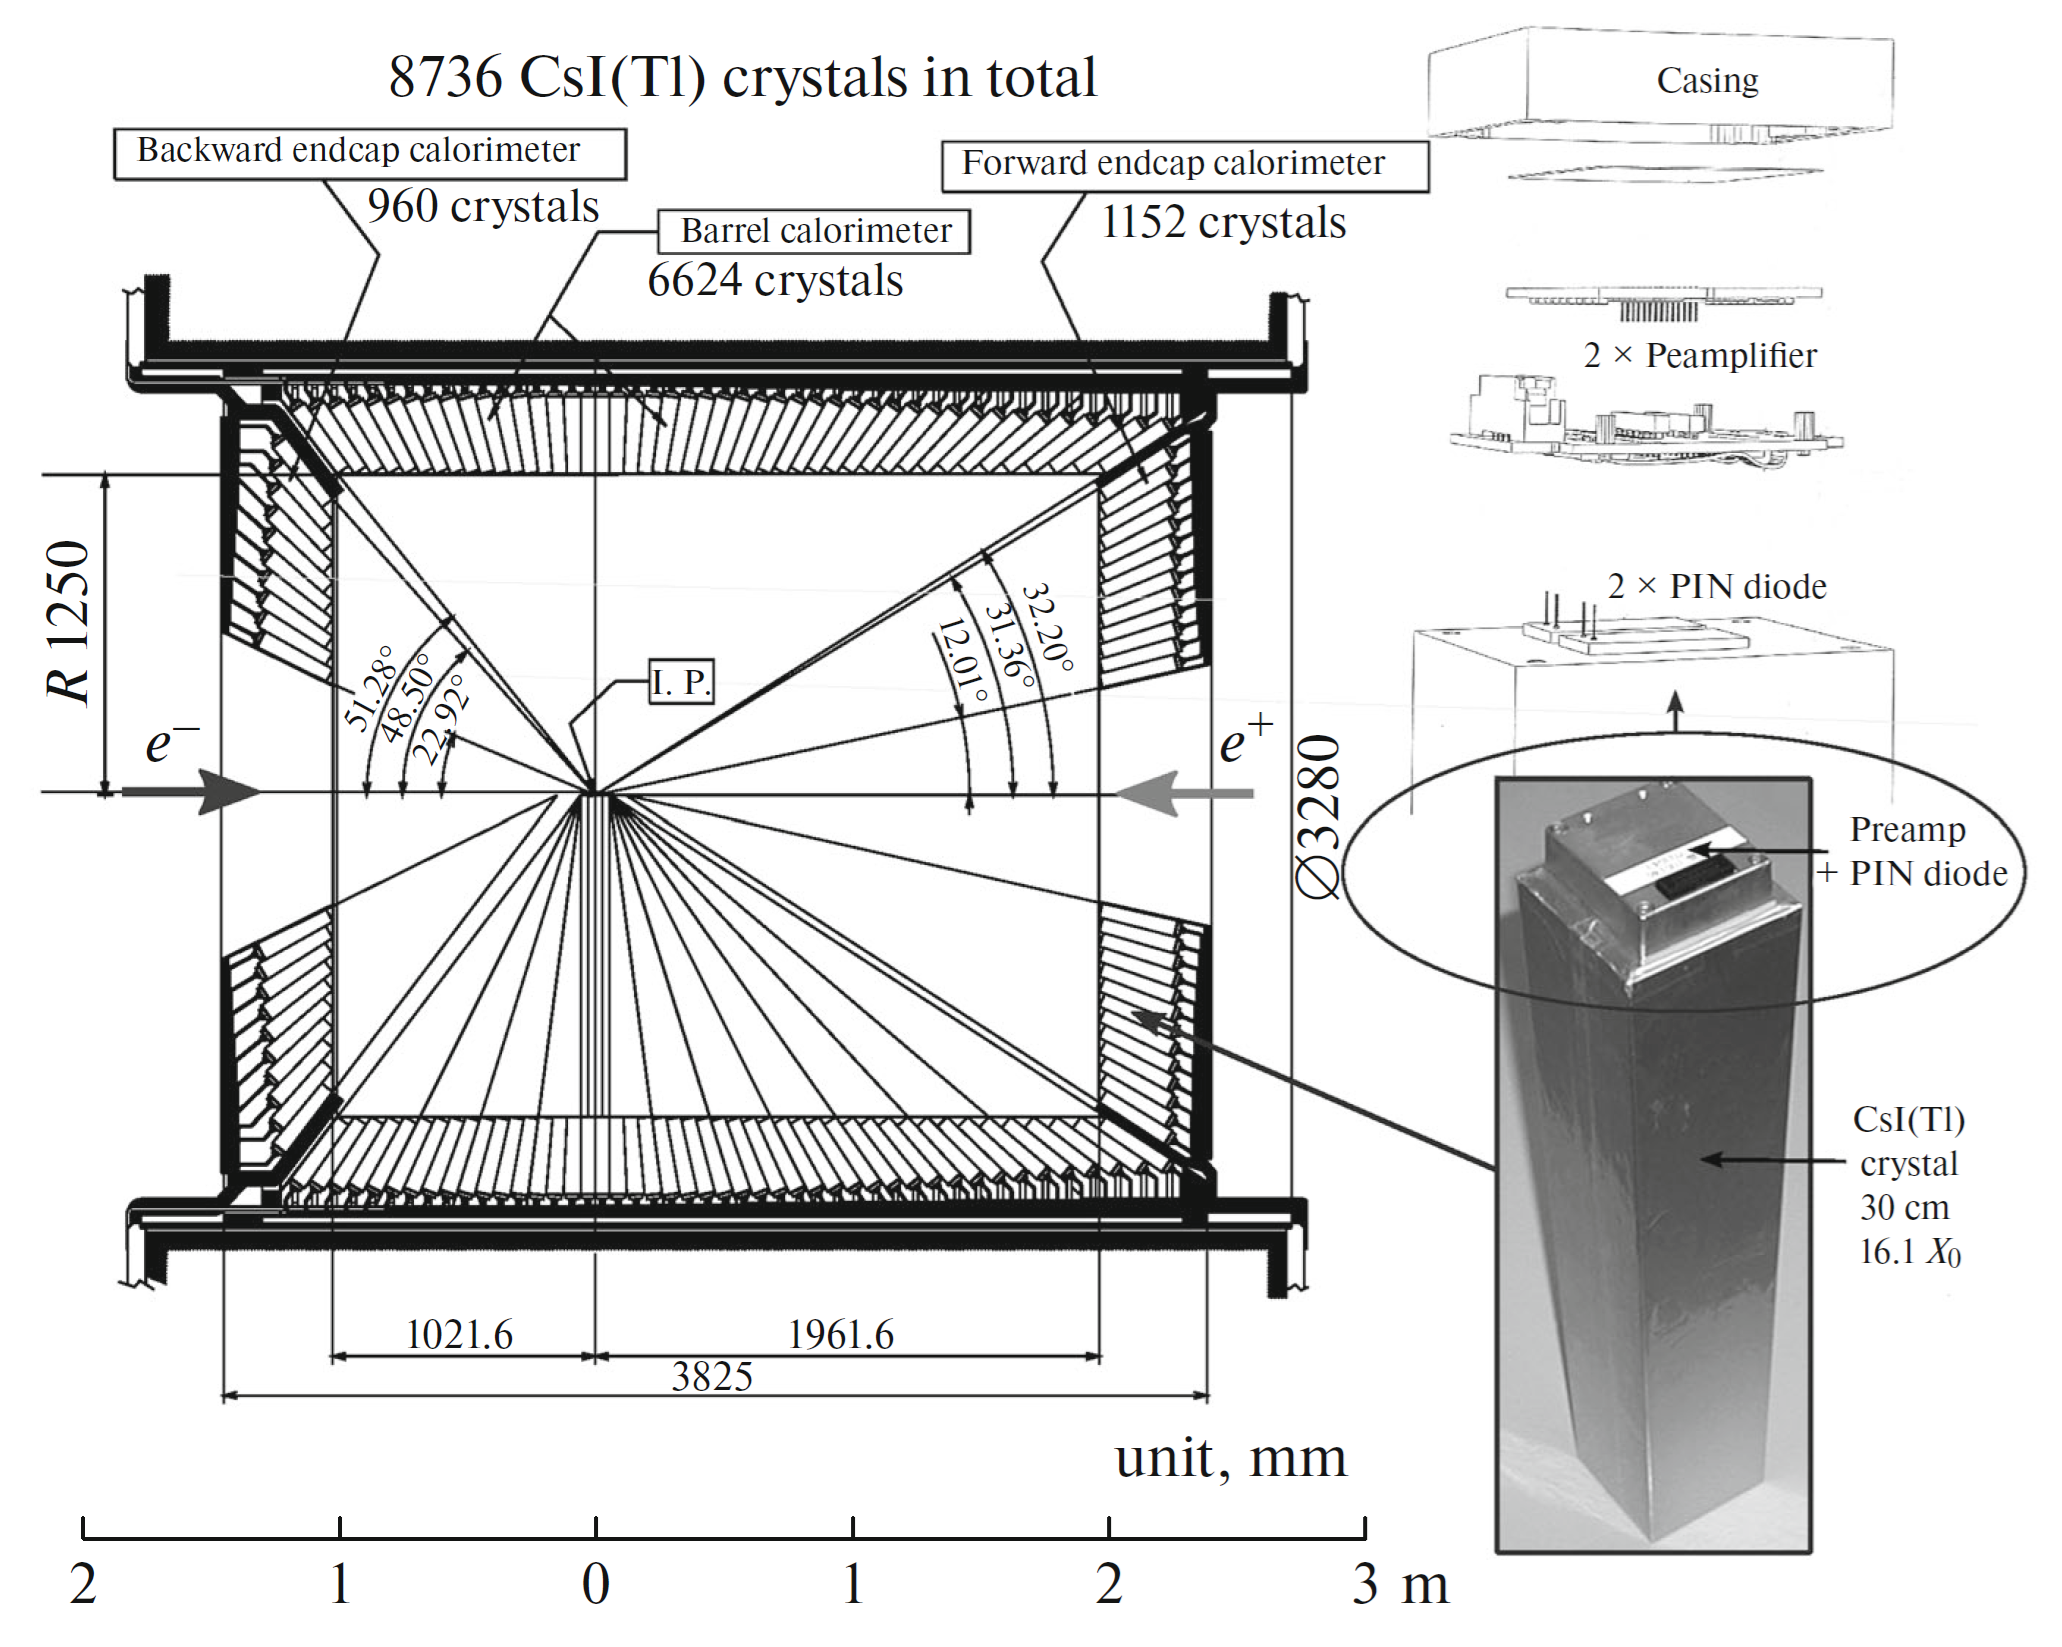
\includegraphics[width=0.65\textwidth]{./picture/ECL.png}
    \caption{(Left) Schematic overview of the ECL. (Right) Schematic overview of the CsI(Tl) crystal.}
    \label{fig:ECL}
\end{figure}

Because the Belle II experiment has higher luminosity than the Belle experiment, more fake clusters are produced by beam particles~\cite{Shebalin:2018sll}.
Using the signal arrival time, these fake clusters can be suppressed.
In the Belle II experiment, the ECL signals are continuously digitized to obtain waveform information.
The waveform is fitted using a known response function to obtain the signal arrival time.

For photons with an energy of $1~\textrm{GeV}$, the ECL achieves a relative energy resolution of $\sigma_E/E = 2.2\%$ and a time resolution of $4~\textrm{ns}$, as measured using $e^{+}e^{-}\to\mu^{+}\mu^{-}\gamma$ events~\cite{Miyabayashi:2025eov}.

\subsection{$K_{L}^{0}$ and $\mu$ detector~(KLM)}
The KLM detector was designed to detect $K_{L}^{0}$ mesons and identify muons.
In the end-cap region, the KLM consists of scintillator strips~\cite{Ketter:2025yqm}.
The scintillation light is collected by wavelength-shifting~(WLS) fibers, and the readout is performed by silicon photomultipliers.
Two orthogonal scintillator layers compose a superlayer, which is covered with an aluminum sheet.
These superlayers are installed between iron plates serving as the magnetic flux return for the solenoid.
There are 26 superlayers in total in the end-cap region: 14 in the forward endcap and 12 in the backward endcap~\cite{Ketter:2025yqm}.
Figure~\ref{fig:EKLM} shows a schematic overview of the scintillator strip and superlayer~\cite{Aushev:2014spa}.
\begin{figure}[h]
    \centering
    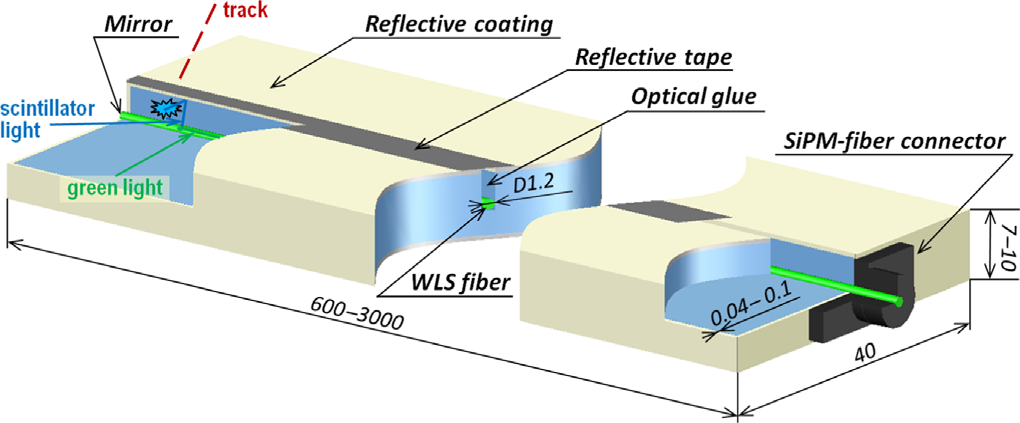
\includegraphics[width=0.45\textwidth]{./picture/KLM_strip.png}
    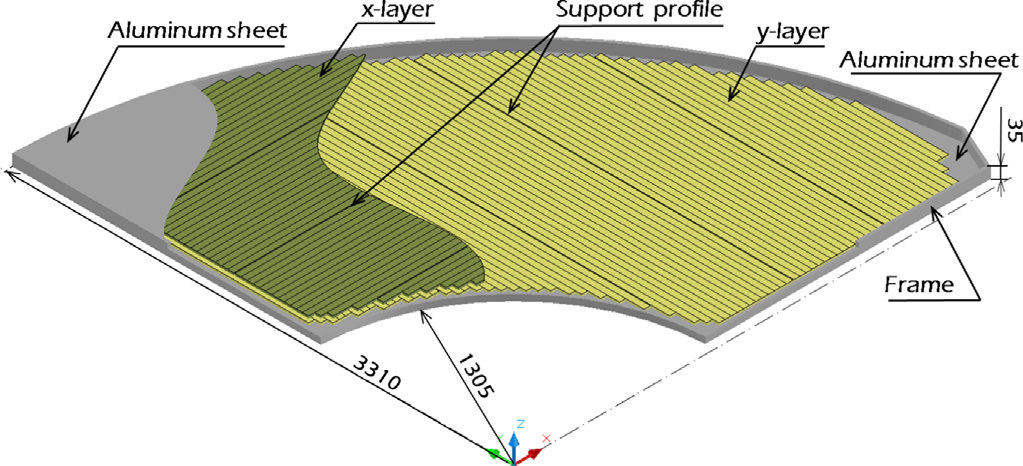
\includegraphics[width=0.45\textwidth]{./picture/KLM.png}
    \caption{(Left) Schematic overview of a scintillator strip. (Right) Schematic overview of a superlayer.}
    \label{fig:EKLM}
\end{figure}

In the barrel region, resistive plate counters~(RPCs) used in the Belle experiment are mainly adopted~\cite{Belle:2000jde}.
During the Belle II upgrade, the two innermost RPC layers were replaced by scintillator layers.
There are 13 RPC layers in the Belle II experiment.

The standard deviations of the hit-time distributions were $7.8~\textrm{ns}$ for RPCs, $5.4~\textrm{ns}$ for barrel scintillators, and $4.7~\textrm{ns}$ for endcap scintillators~\cite{Ketter:2025yqm}.
Muon identification uses the penetration depth and transverse hit distribution in the KLM, together with information from the other particle-identification detectors.
For momenta above $1~\textrm{GeV}/c$, the combined identification achieves a muon efficiency above $90\%$ with a pion misidentification probability of approximately $5\%$~\cite{Belle-II:2026okl}.

\subsection{Trigger and data acquisition systems}
To meet the hardware limitations, data must be recorded selectively while keeping physically interesting events.
The first stage of the trigger system is called the Level-1 trigger.
In the Level-1 trigger, a trigger efficiency close to 100\% is required for hadronic events, while keeping the trigger rate below 30~kHz~\cite{Lai:2025gac}.
The Level-1 trigger consists of sub-triggers, global reconstruction logic~(GRL), and global decision logic~(GDL).
Figure~\ref{fig:L1_trigger} shows a schematic overview of the Level-1 trigger~\cite{Lai:2025gac}.
\begin{figure}[h]
    \centering
    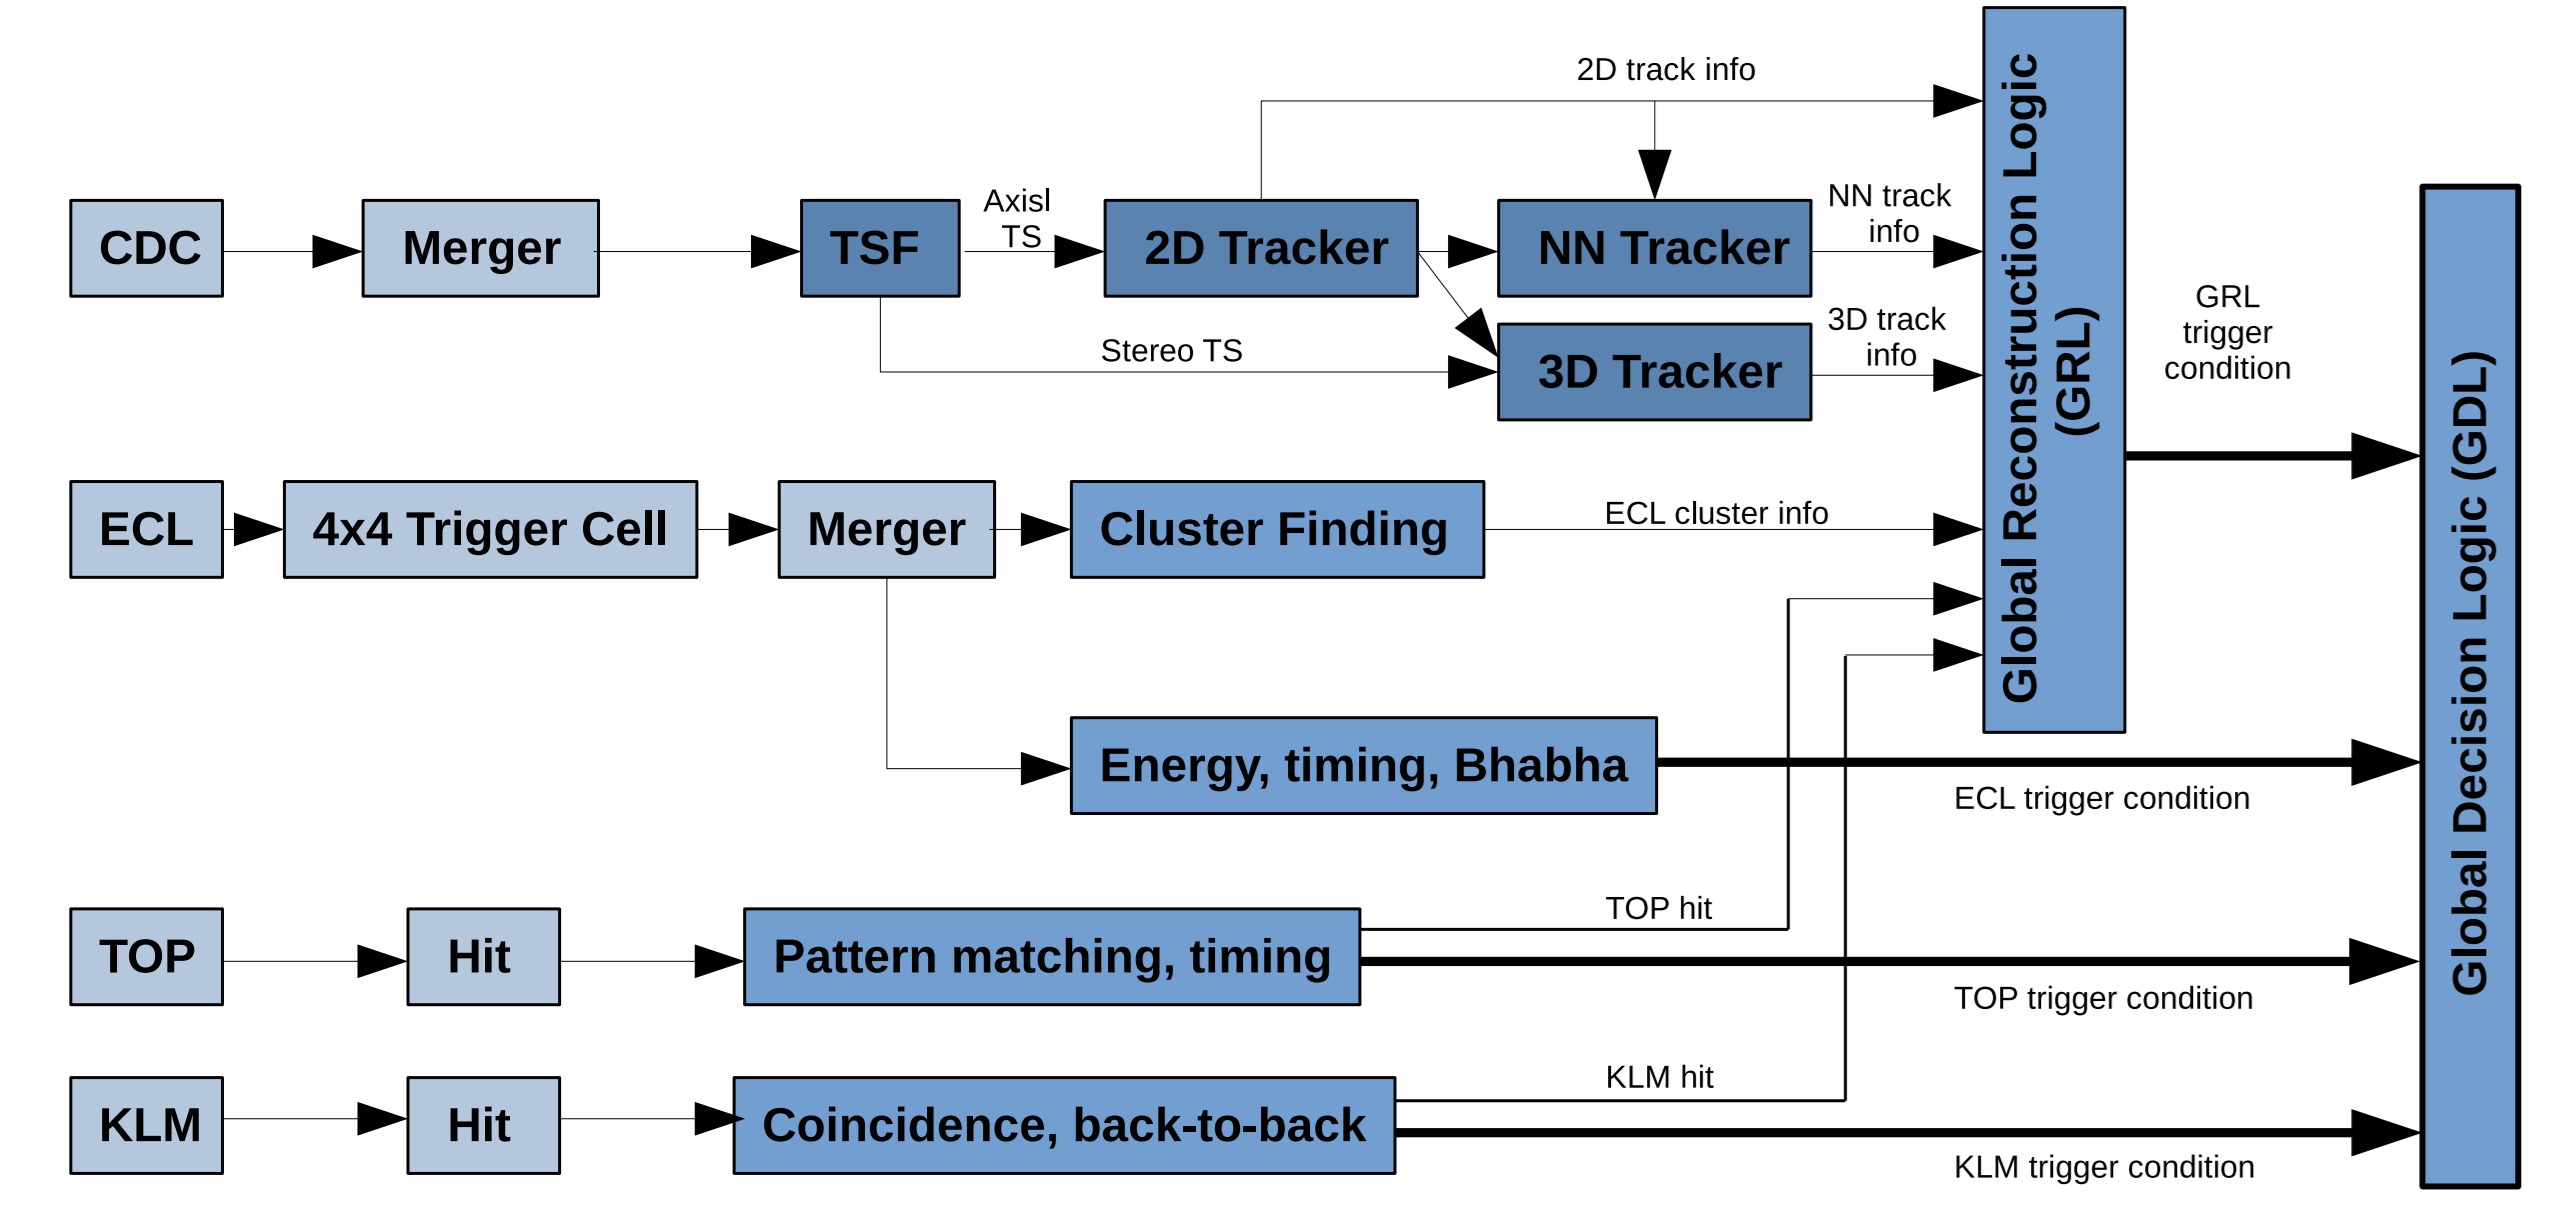
\includegraphics[width=0.85\textwidth]{./picture/L1_trigger.png}
    \caption{Schematic overview of the Level-1 trigger.}
    \label{fig:L1_trigger}
\end{figure}
There are four sub-triggers: CDC, ECL, TOP, and KLM triggers.
The GRL receives information from the four sub-triggers and analyzes the event topology.
The GDL receives information from the GRL and the sub-triggers and produces output bits.

After an event is accepted by the Level-1 trigger, the detector signals are sent to the readout PCs.
The event builder combines detector data to form one collision event~\cite{Nakao:2020lva}.
A high-level trigger~(HLT) uses the Belle II Analysis Software Framework~\cite{Kuhr:2018lps} to reconstruct the events~\cite{Braun:2020otr}.
The HLT determines whether to retain or discard the reconstructed events.
At the SuperKEKB design luminosity of $8\times10^{35}~\textrm{cm}^{-2}\textrm{s}^{-1}$~\cite{Akai:2018mbz}, the expected recording rate after HLT selection is $10~\textrm{kHz}$, with a raw-data event size of approximately $200~\textrm{kB}$~\cite{Braun:2020otr}.

\chapter{Software and Data Samples}

\section{Software}
The Belle II software framework~(\textsc{basf2})~\cite{Kuhr:2018lps} is used to reconstruct events.
The \textsc{basf2} version used in this analysis is \texttt{light-2305-korat}.
\textsc{basf2} produces ROOT files~\cite{Brun:1997pa} that include kinematic and event information.
To analyze these ROOT files, the ROOT data analysis framework is used.

For Monte Carlo~(MC) sample generation, \textsc{EvtGen}~\cite{Lange:2001uf} is used to simulate $B$- and $D$-meson decay chains.
\textsc{KKMC}~\cite{Jadach:1999vf} is used to simulate $e^{+}e^{-}\to q\bar{q}$ events. \textsc{PHOTOS}~\cite{Barberio:1990ms} is used to simulate photon radiation from charged particles.
\textsc{Pythia8}~\cite{Sjostrand:2014zea} is used to simulate quark fragmentation.
\textsc{Geant4}~\cite{Agostinelli:2002hh} is used to simulate the detector response.

\section{Monte Carlo samples}
To avoid human bias, the data collected from the Belle II experiment are not analyzed before the analysis procedure is determined.
Before checking the data, the analysis procedure is optimized using MC samples.

\subsection{Background Monte Carlo samples}
\label{subsec:backgroundMC}
The background MC samples used in this analysis include samples produced centrally by the Belle II collaboration and samples generated specifically for this analysis, referred to as private MC samples.
The centrally produced samples belong to the MC15 production campaign and comprise run-independent~(MC15ri) and run-dependent~(MC15rd) samples.
Here, a run refers to a period of data taking under approximately stable operating conditions.
The MC15ri samples use common simulation conditions across runs, whereas the MC15rd samples account for variations in detector conditions and beam backgrounds between runs.

Both MC15ri and MC15rd samples generated at the $\Upsilon(4S)$ resonance are used.
These are referred to as on-resonance samples.
These samples include $e^{+}e^{-}\to\Upsilon(4S)\to B\bar{B}$ and $e^{+}e^{-}\to q\bar{q}$~($q=u,d,s,c$) events.
Off-resonance MC15rd samples, generated at a center-of-mass energy $60~\mathrm{MeV}$ below the resonance, are also used.
They consist of $e^{+}e^{-}\to q\bar{q}$ events.

The private MC samples are generated at the $\Upsilon(4S)$ resonance and consist of $B^{+}\to K^{+}n\bar{n}$, $B^{+}\to K^{*+}n\bar{n}$, $B^{0}\to K^{0}n\bar{n}$, and $B^{0}\to K^{*0}n\bar{n}$ events.

The official on-resonance MC15ri samples are used to train a boosted decision tree (BDT)~\cite{Keck:2017gsv} and check for overfitting.
The official on-resonance MC15rd and private MC samples are used to obtain the histogram templates.

The off-resonance MC15rd samples are used to estimate the correction factor and its systematic uncertainty for $e^{-}e^{+}\rightarrow q\bar{q}$ events.

Table~\ref{tab:MC_background} shows the integrated luminosities or numbers of events for the background MC samples.
\begin{table}
    \caption{Integrated luminosities or numbers of events of the background MC samples used in the analysis.}
    \centering
    \begin{tabular}{ p{5cm} p{5cm} p{5cm} p{5cm} p{5cm}  }
    \hline
    \hline
    \multicolumn{1}{c}{Background type} & \multicolumn{1}{c}{Version} & \multicolumn{1}{c}{Energy} & \multicolumn{1}{c}{Luminosity~($\textrm{fb}^{-1}$)} & \multicolumn{1}{c}{Number of events} \\
    \hline
    \multicolumn{1}{c}{$e^{+}e^{-}\to \Upsilon(4S) \to B\bar{B}$} & \multicolumn{1}{c}{MC15ri} & \multicolumn{1}{c}{on-resonance} & \multicolumn{1}{c}{2800} & \multicolumn{1}{c}{-}\\
    \multicolumn{1}{c}{$e^{+}e^{-} \to q\bar{q}$} & \multicolumn{1}{c}{MC15ri} & \multicolumn{1}{c}{on-resonance} & \multicolumn{1}{c}{1000} & \multicolumn{1}{c}{-}\\
    \multicolumn{1}{c}{$B^{+}\to K^{+}n\bar{n}$} & \multicolumn{1}{c}{-} & \multicolumn{1}{c}{on-resonance} & \multicolumn{1}{c}{-} & \multicolumn{1}{c}{20000}\\
    \multicolumn{1}{c}{$B^{+}\to K^{*+}n\bar{n}$} & \multicolumn{1}{c}{-} & \multicolumn{1}{c}{on-resonance} & \multicolumn{1}{c}{-} & \multicolumn{1}{c}{20000}\\
    \multicolumn{1}{c}{$B^{0}\to K^{0}n\bar{n}$} & \multicolumn{1}{c}{-} & \multicolumn{1}{c}{on-resonance} & \multicolumn{1}{c}{-} & \multicolumn{1}{c}{20000}\\
    \multicolumn{1}{c}{$B^{0}\to K^{*0}n\bar{n}$} & \multicolumn{1}{c}{-} & \multicolumn{1}{c}{on-resonance} & \multicolumn{1}{c}{-} & \multicolumn{1}{c}{20000}\\
    \multicolumn{1}{c}{$e^{+}e^{-}\to \Upsilon(4S) \to B\bar{B}$} & \multicolumn{1}{c}{MC15rd} & \multicolumn{1}{c}{on-resonance} & \multicolumn{1}{c}{1458.959} & \multicolumn{1}{c}{-}\\
    \multicolumn{1}{c}{$e^{+}e^{-} \to q\bar{q}$} & \multicolumn{1}{c}{MC15rd} & \multicolumn{1}{c}{on-resonance} & \multicolumn{1}{c}{1458.959} & \multicolumn{1}{c}{-}\\
    \multicolumn{1}{c}{$e^{+}e^{-} \to q\bar{q}$} & \multicolumn{1}{c}{MC15rd} & \multicolumn{1}{c}{off-resonance} & \multicolumn{1}{c}{169.328} & \multicolumn{1}{c}{-}\\
  \hline
  \hline
\end{tabular}
    \label{tab:MC_background}
\end{table}

The official $B\to X_{s}n\bar{n}$ MC samples are generated using a flat phase-space model, in which the decay products are distributed uniformly in phase space.
However, studies of $B\to K^{(*)}p\bar{p}$ show $M_{p\bar{p}}$ distributions that differ from the flat phase-space distribution~\cite{Belle:2007oni,Belle:2008zkc,BaBar:2007esv}.
Because $B\to K^{(*)}n\bar{n}$ has a detector response similar to that of $B\to K^{(*)}\nu\bar{\nu}$ decays, dedicated modeling is needed.
Therefore, direct $B\to K^{(*)}n\bar{n}$ decays without the $J/\psi$ resonance are removed from the official MC15rd samples and private $B\to K^{(*)}n\bar{n}$ samples are produced.
For the private $B\to K^{(*)}n\bar{n}$ samples, a flat $M_{n\bar{n}}$ distribution is required.
The details of the correction for the $M_{n\bar{n}}$ distribution are discussed in Section~\ref{sec:Xsnnbar_correction}.

\subsection{Signal Monte Carlo samples}
\label{subsec:signal_MC}
Separate signal MC samples are generated for three components: $B\to K\nu\bar{\nu}$, $B\to K^{*}\nu\bar{\nu}$, and $B\to X_s\nu\bar{\nu}$ excluding the $K$ and $K^{*}$ modes.

For the $B\rightarrow K \nu \bar{\nu}$ sample, the following parameters are used in Eq.~\ref{eq:Knunu_formfactor}~\cite{Buras:2014fpa}:
\begin{equation}
  \begin{aligned}
    \alpha_0 &= 0.432 \pm 0.011, \\
    \alpha_1 &= -0.664 \pm 0.096, \\
    \alpha_2 &= -1.20 \pm 0.69.
  \end{aligned}
\end{equation}
During the analysis, updated parameter values were published~\cite{Parrott:2022rgu}:
\begin{equation}
  \label{eq:coeff_Kff}
  \begin{aligned}
    \alpha_0 &= 0.2545 \pm 0.0090, \\
    \alpha_1 &= -0.71 \pm 0.14, \\
    \alpha_2 &= 0.32 \pm 0.59.
  \end{aligned}
\end{equation}
Therefore, the generated $B\rightarrow K\nu\bar{\nu}$ sample is reweighted.
This reweighting is applied to the $d\Gamma/dq^{2}$ distribution~\cite{Buras:2014fpa}:
\begin{equation}
  \frac{d\Gamma}{dq^{2}} \propto
  \left[\lambda(m_{B}^{2},m_{K}^{2},q^{2})\right]^{3/2}
  \left[f_{+}(q^{2})\right]^{2}.
\end{equation}

For the $B\rightarrow K^{*}\nu \bar{\nu}$ sample, the following parameters are used in Eq.~\ref{eq:Kstarnunu_formfactor}~\cite{Bharucha:2015bzk}:
\begin{equation}
  \label{eq:Kstnunu_alpha}
  \begin{aligned}
    \alpha_{0}^{V} &= 0.39 \pm 0.03, &
    \alpha_{0}^{A_{1}} &= 0.30 \pm 0.03, &
    \alpha_{0}^{A_{12}} &= 0.27 \pm 0.02, \\
    \alpha_{1}^{V} &= -1.17 \pm 0.26, &
    \alpha_{1}^{A_{1}} &= 0.39 \pm 0.19, &
    \alpha_{1}^{A_{12}} &= 0.53 \pm 0.13, \\
    \alpha_{2}^{V} &= 2.42 \pm 1.53, &
    \alpha_{2}^{A_{1}} &= 1.19 \pm 1.03, &
    \alpha_{2}^{A_{12}} &= 0.48 \pm 0.66.
  \end{aligned}
\end{equation}

For the $B\to X_s\nu\bar{\nu}$ component excluding the $K$ and $K^{*}$ modes, Eq.~\ref{eq:Xsamp} is used to simulate the $q^{2}$ distribution. 
However, this equation does not determine the mass of $X_{s}$.
Therefore, the Fermi motion model~\cite{Ali:1996bm} is adopted to produce the $B\rightarrow X_{s} \nu \bar{\nu}$ sample.
In the Fermi motion model, inside the $B$ meson, $b$ quark and spectator quark have four-momenta $p$ and $p_{\textrm{spectator}}$, respectively.
The probability density function for the momentum is
\begin{equation}
  \label{eq:p_pdf}
  \phi(p) = \frac{4}{\sqrt{\pi} p_{F}^{3}} \exp(\frac{-p^2}{p_{F}^{2}}),
\end{equation}
where $p_{F}$ is the Fermi motion momentum, $p = \left| \vec{p} \right|$ is the magnitude of the momentum of the $b$ quark~\cite{Ali:1996bm}, which satisfies $\int_{0}^{\infty}dp~p^{2} \phi(p) = 1$.
The Fermi motion momentum satisfies the following equation for a spectator-quark mass of $m_{\mathrm{sp}}\sim0~\mathrm{GeV}/c^2$~\cite{Kim:1998wx}:
\begin{equation}
  \label{eq:mu_pi}
  \mu_{\pi}^{2}=6p_{F}^{2}-3\left<p \right>^{2}_{B-rest},
\end{equation}
where $\mu_{\pi}^{2}=0.464\pm0.076~\textrm{GeV}^{2}$~\cite{HFLAV:2022pwe} is the average kinetic energy of $b$–quark.
From Eq.~\ref{eq:p_pdf},
\begin{equation}
  \label{eq:p_B_rest}
  \left<p \right>_{B-rest} = \int^{\infty}_{0}p^{2} \phi(p) p dp = \frac{2}{\sqrt{\pi}} p_{F}.
\end{equation}
By substituting Eq.~\ref{eq:p_B_rest} into Eq.~\ref{eq:mu_pi} with $\mu_{\pi}^{2}=0.464\pm0.076~\textrm{GeV}^{2}$, we obtain
\begin{equation}
  \label{eq:pf}
  p_{F} = 0.461^{+0.036}_{-0.039}~\textrm{GeV}/c.
\end{equation}
With this value of the Fermi motion momentum, the momentum of the $s$-quark is determined from the momentum of $b$-quark.
Then the mass of $X_{s}$ can be calculated as follows:
\begin{equation}
  M_{X_{s}}^{2} = \left( p_{\textrm{s}} + p_{\textrm{spectator}}  \right)^{2},
\end{equation}
where $p_{\textrm{s}}$ is the momentum of $s$-quark and $p_{\textrm{spectator}}$ is the momentum of spectator quark in the $B$ meson.
Here, the mass of $X_{s}$ is required to satisfy $M_{X_{s}} > 1.1~\textrm{GeV}/c^{2}$.
This mass threshold is motivated by the $X_{s}$ mass distribution in $B \rightarrow X_s\gamma$ decays~\cite{Belle:2014nmp}.
In addition, studies of $B^{+} \rightarrow K^{+}\pi^{+}\pi^{-}\mu^{+}\mu^{-}$ and $B^{0} \rightarrow K^{+}\pi^{-}\mu^{+}\mu^{-}$ decays show that no significant contribution is observed below this mass threshold, except for the $K^{*}$ resonance~\cite{LHCb:2016ykl,LHCb:2014osj}.
After determining the kinematics of the $X_{s}\nu \bar{\nu}$ decay, the hadronization is performed using \textsc{Pythia8}~\cite{Sjostrand:2014zea}.

Figures~\ref{fig:q2_KandKstar} and~\ref{fig:q2_K_reweighted} show the $q^{2}$ distribution for the MC samples and theoretical calculations.
\begin{figure}[h]
    \centering
    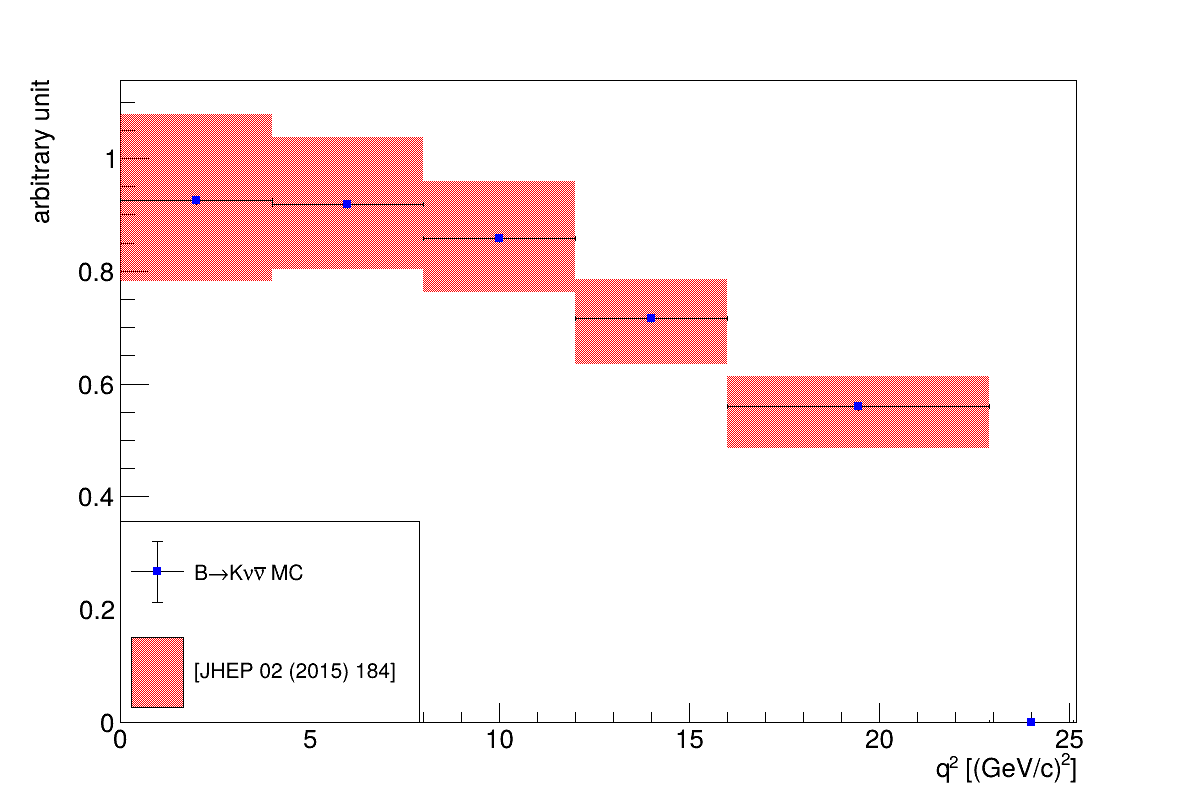
\includegraphics[width=0.48\textwidth]{./picture/Knunu_q2distribution_old.png}
    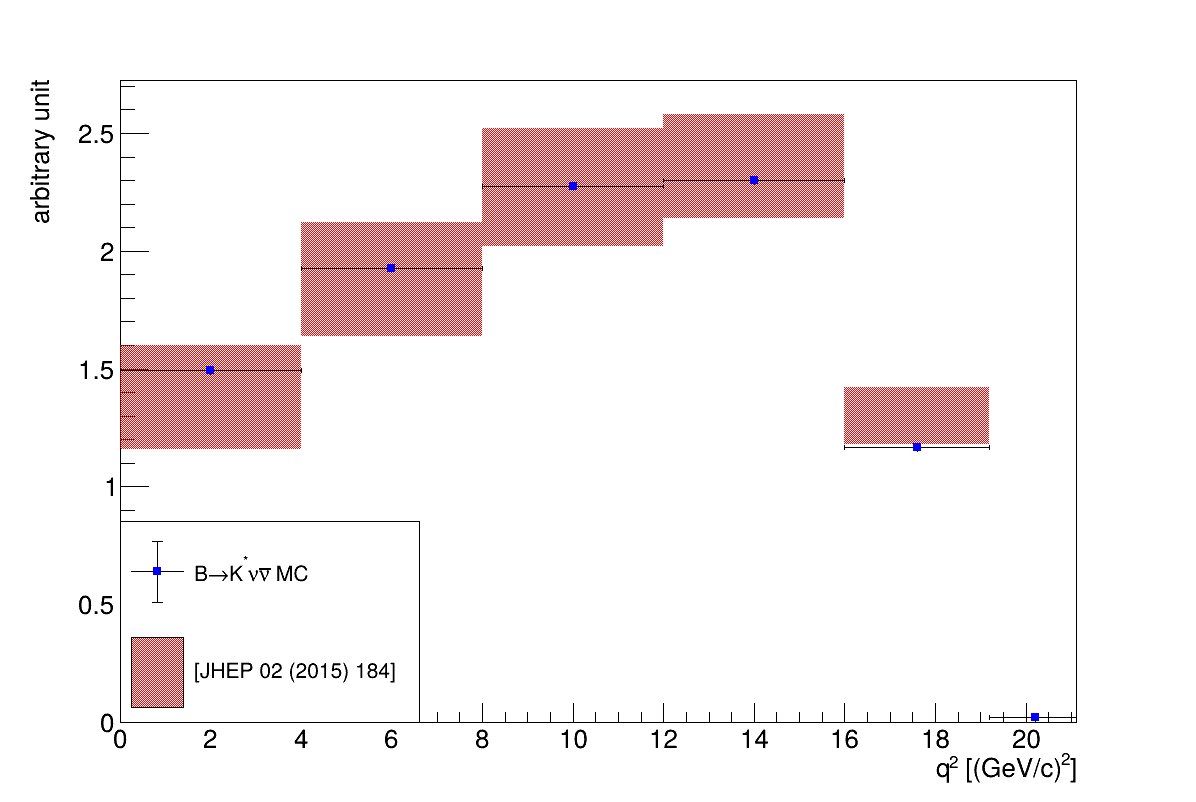
\includegraphics[width=0.48\textwidth]{./picture/Kstarnunu_q2distribution.png}
    \caption{$q^{2}$ distributions for the (left) $B\to K\nu\bar{\nu}$ and (right) $B\to K^{*}\nu\bar{\nu}$ MC samples, compared with the Standard Model predictions~\cite{Buras:2014fpa}. The blue points show the MC distributions, and the red bands indicate the theoretical uncertainties of the predictions in each $q^{2}$ bin.}
    \label{fig:q2_KandKstar}
\end{figure}
\begin{figure}[h]
    \centering
    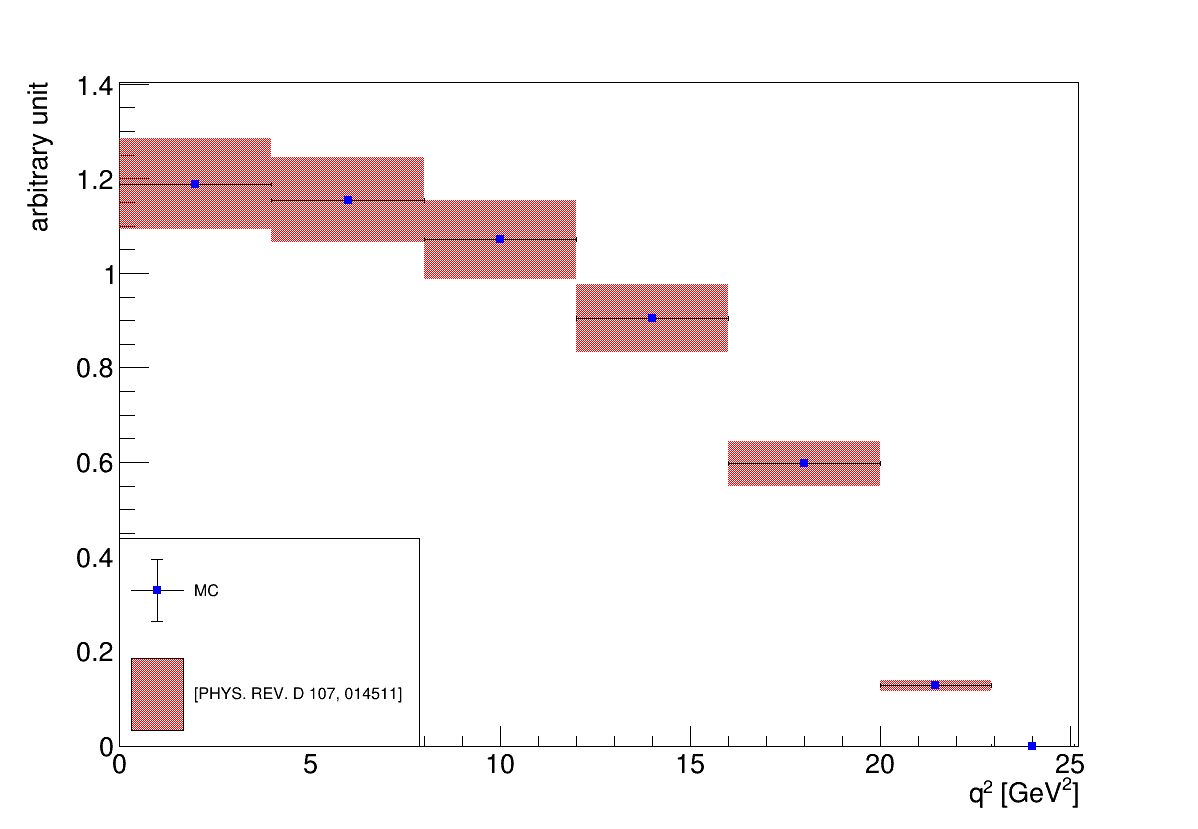
\includegraphics[width=0.48\textwidth]{./picture/Knunu_q2distribution_new.png}
    \caption{$q^{2}$ distribution for the reweighted $B\to K\nu\bar{\nu}$ MC sample, compared with the Standard Model prediction~\cite{Parrott:2022zte}. The blue points show the reweighted MC distribution, and the red bands indicate the theoretical uncertainties of the prediction in each $q^{2}$ bin.}
    \label{fig:q2_K_reweighted}
\end{figure}
For $B\to K^{*}\nu\bar{\nu}$, the MC distribution differs from the central values of the theoretical prediction in several $q^{2}$ bins, as shown in Figure~\ref{fig:q2_KandKstar} (right).
These differences arise from the finite width of the $K^{*}$ resonance included in the MC simulation, whereas the theoretical calculation assumes a fixed $K^{*}$ mass.
This was verified by fixing the $K^{*}$ mass in the MC simulation, which brought the $q^{2}$ distribution into agreement with the central values of the theoretical prediction.
Since the finite width reflects the physical nature of the $K^{*}$ resonance, the MC distribution is retained without additional $q^{2}$ reweighting.

When combining $B^{+}B^{-}$ and $B^{0}\bar{B}^{0}$ samples, we use the following relation:
\begin{equation}
  \begin{aligned}
      N_{B^{+}B^{-}}&=N_{\Upsilon(4S)}\cdot f^{+-},\\
      N_{B^{0}\bar{B}^{0}}&=N_{\Upsilon(4S)}\cdot f^{00},
  \end{aligned}
\end{equation}
where $f^{+-}=0.5113^{+0.0073}_{-0.0108}$, $f^{00}=0.4861^{+0.0074}_{-0.0080}$~\cite{HeavyFlavorAveragingGroupHFLAV:2024ctg}, $N_{\Upsilon(4S)}$ is the number of $\Upsilon(4S)$ events, $N_{B^{+}B^{-}}$ is the number of $B^{+}B^{-}$ pairs, and $N_{B^{0}\bar{B}^{0}}$ is the number of $B^{0}\bar{B}^{0}$ pairs.
To combine the three signal components, we use $BR(B^{+}\to K^{+}\nu\bar{\nu}) = 5.044\times10^{-6}$, $BR(B^{0}\to K^{*0}\nu\bar{\nu}) = 9.19\times10^{-6}$, and $BR(B\to X_s\nu\bar{\nu}) = 2.9\times10^{-5}$ ~\cite{Buras:2014fpa,Parrott:2022zte}.
The branching ratios for the charged and neutral exclusive modes are related by~\cite{Buras:2014fpa}:
\begin{equation}
  \begin{aligned}
      \frac{BR(B^{+}\rightarrow K^{(*)+}\nu \bar{\nu})}{BR(B^{0}\rightarrow K^{(*)0}\nu \bar{\nu})} = \frac{\tau_{B^{+}}}{\tau_{B^{0}}},
  \end{aligned}
\end{equation}
where $\tau_{B^{+}}$ and $\tau_{B^{0}}$ are the lifetimes of the $B^{+}$ and $B^{0}$ mesons, respectively.
For the component excluding the $K$ and $K^{*}$ modes, the branching ratios are obtained by subtracting these exclusive contributions from the inclusive prediction.
We denote this component by the subscript $X_{s}\neq K,K^{*}$:
\begin{equation}
\begin{aligned}
  BR(B^{+}\rightarrow X_s \nu \bar{\nu})_{X_{s}\neq K,K^{*}} &= BR(B\rightarrow X_{s}\nu \bar{\nu}) - BR(B^{+}\rightarrow K^{+}\nu \bar{\nu}) - BR(B^{+}\rightarrow K^{*+}\nu \bar{\nu})\\
  &= 2.9 \times 10^{-5} - 5.044 \times 10^{-6} - 9.91 \times 10^{-6}\\
  &= 1.405 \times 10^{-5},
\end{aligned}
\end{equation}
\begin{equation}
\begin{aligned}
  BR(B^{0}\rightarrow X_s \nu \bar{\nu})_{X_{s}\neq K,K^{*}} &= BR(B\rightarrow X_{s}\nu \bar{\nu}) - BR(B^{0}\rightarrow K^{0}\nu \bar{\nu}) - BR(B^{0}\rightarrow K^{*0}\nu \bar{\nu})\\
  &= 2.9 \times 10^{-5} - 3.69 \times 10^{-6} - 9.19 \times 10^{-6}\\
  &= 1.513 \times 10^{-5}.
\end{aligned}
\end{equation}

Figure~\ref{fig:fragmentation} shows the fragmentation of $X_{s}$ in the entire $B\rightarrow X_{s} \nu \bar{\nu}$ signal MC sample.
$K$ in the legend denotes charged and neutral kaons.
$\pi$ in the legend denotes charged pions only.
The ``other" category includes decay modes such as $B\rightarrow K\eta\nu\bar{\nu}$.
\begin{figure}[h]
    \centering
    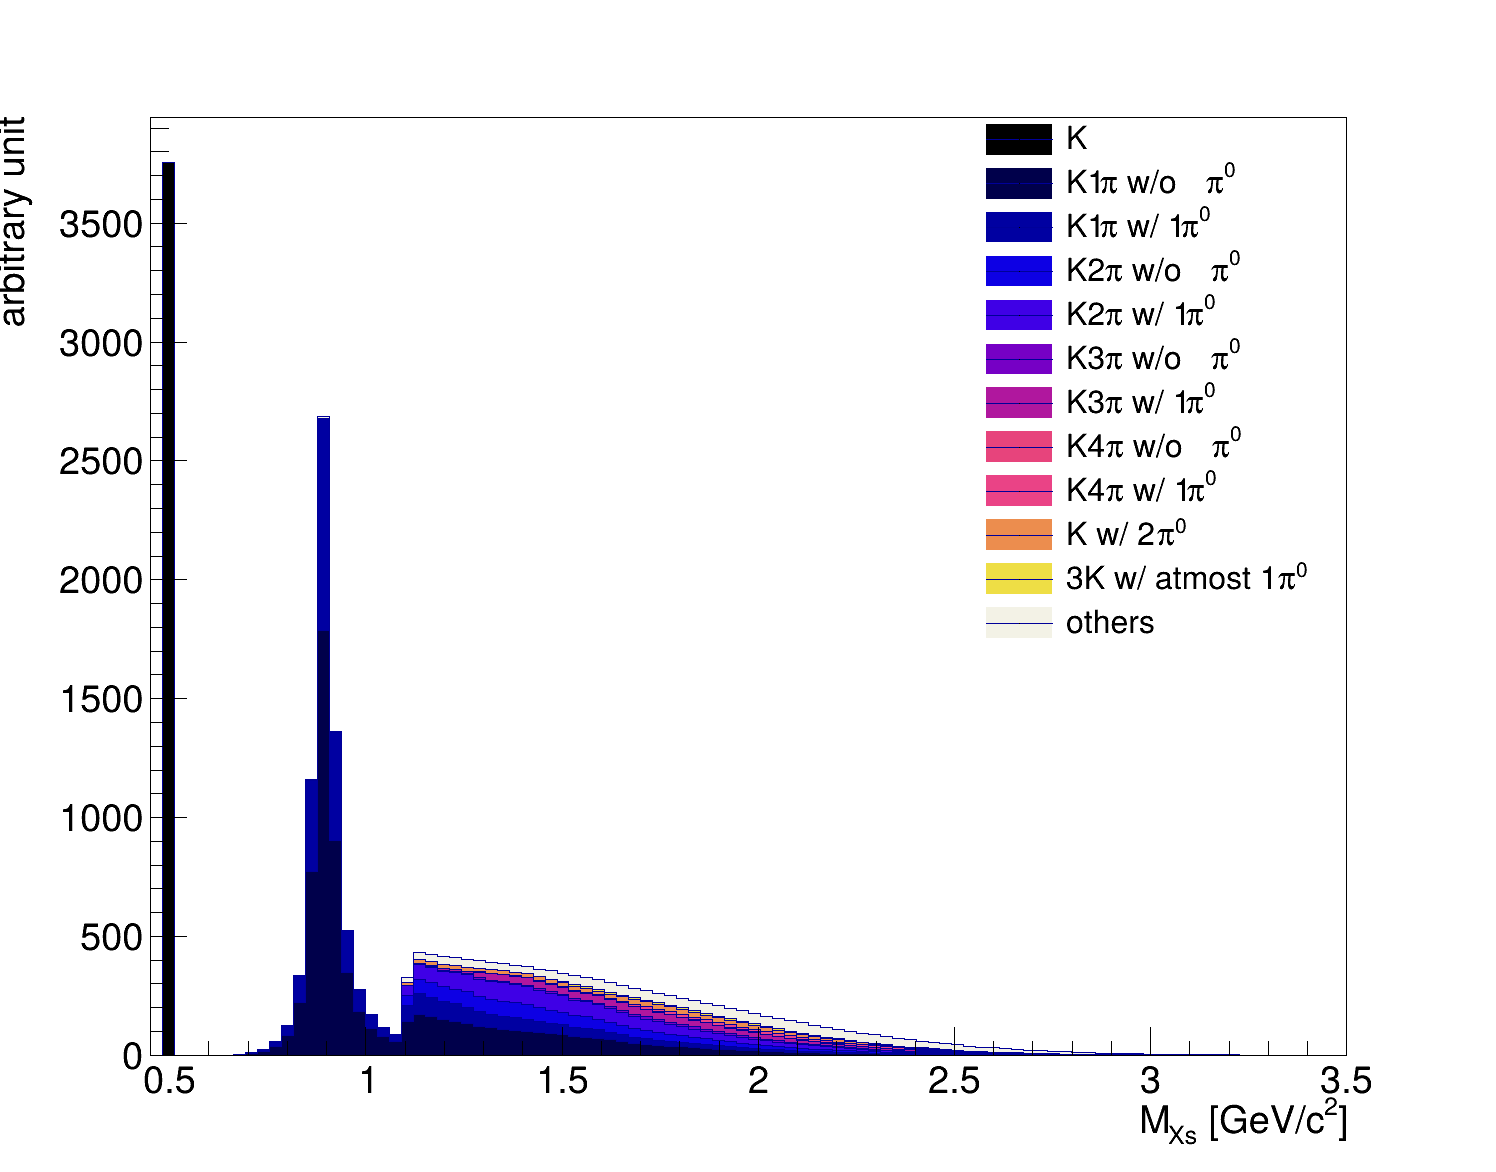
\includegraphics[width=0.80\textwidth]{./picture/Mxs_legend.png}
    \caption{Fragmentation of $X_{s}$ in the entire $B\rightarrow X_{s} \nu \bar{\nu}$ signal MC sample. $K$ in the legend denotes charged and neutral kaons. $\pi$ in the legend denotes charged pions only. The "other" category includes decay modes such as $B\rightarrow K\eta\nu\bar{\nu}$.}
    \label{fig:fragmentation}
\end{figure}

Table~\ref{tab:MC_signal} shows the numbers of events in the signal MC samples.
\begin{table}
\caption{Numbers of events in the signal MC samples used in the analysis.}
    \centering
    \begin{tabular}{ p{5cm} p{5cm} p{5cm} p{5cm}  }
    \hline
    \hline
    \multicolumn{1}{c}{Signal type} & \multicolumn{1}{c}{Version} & \multicolumn{1}{c}{Energy} & \multicolumn{1}{c}{Number of events} \\
    \hline
    \multicolumn{1}{c}{$B^{+}\rightarrow K^{+} \nu \bar{\nu}$} & \multicolumn{1}{c}{MC15ri} & \multicolumn{1}{c}{on-resonance} & \multicolumn{1}{c}{$10^{7}$}\\
    \multicolumn{1}{c}{$B^{+}\rightarrow K^{*+} \nu \bar{\nu}$} & \multicolumn{1}{c}{MC15ri} & \multicolumn{1}{c}{on-resonance} & \multicolumn{1}{c}{$10^{7}$}\\
    \multicolumn{1}{c}{Remaining $B^{+}\rightarrow X_{s} \nu \bar{\nu}$} & \multicolumn{1}{c}{MC15ri} & \multicolumn{1}{c}{on-resonance} & \multicolumn{1}{c}{$5 \times 10^{7}$}\\
    \multicolumn{1}{c}{$B^{0}\rightarrow K^{0} \nu \bar{\nu}$} & \multicolumn{1}{c}{MC15ri} & \multicolumn{1}{c}{on-resonance} & \multicolumn{1}{c}{$10^{7}$}\\
    \multicolumn{1}{c}{$B^{0}\rightarrow K^{*0} \nu \bar{\nu}$} & \multicolumn{1}{c}{MC15ri} & \multicolumn{1}{c}{on-resonance} & \multicolumn{1}{c}{$10^{7}$}\\
    \multicolumn{1}{c}{Remaining $B^{0}\rightarrow X_{s} \nu \bar{\nu}$} & \multicolumn{1}{c}{MC15ri} & \multicolumn{1}{c}{on-resonance} & \multicolumn{1}{c}{$5 \times 10^{7}$}\\
    \multicolumn{1}{c}{$B^{+}\rightarrow K^{+} \nu \bar{\nu}$} & \multicolumn{1}{c}{MC15rd} & \multicolumn{1}{c}{on-resonance} & \multicolumn{1}{c}{3962022}\\
    \multicolumn{1}{c}{$B^{+}\rightarrow K^{*+} \nu \bar{\nu}$} & \multicolumn{1}{c}{MC15rd} & \multicolumn{1}{c}{on-resonance} & \multicolumn{1}{c}{3962022}\\
    \multicolumn{1}{c}{Remaining $B^{+}\rightarrow X_{s} \nu \bar{\nu}$} & \multicolumn{1}{c}{MC15rd} & \multicolumn{1}{c}{on-resonance} & \multicolumn{1}{c}{15846594}\\
    \multicolumn{1}{c}{$B^{0}\rightarrow K^{0} \nu \bar{\nu}$} & \multicolumn{1}{c}{MC15rd} & \multicolumn{1}{c}{on-resonance} & \multicolumn{1}{c}{3962022}\\
    \multicolumn{1}{c}{$B^{0}\rightarrow K^{*0} \nu \bar{\nu}$} & \multicolumn{1}{c}{MC15rd} & \multicolumn{1}{c}{on-resonance} & \multicolumn{1}{c}{3962022}\\
    \multicolumn{1}{c}{Remaining $B^{0}\rightarrow X_{s} \nu \bar{\nu}$} & \multicolumn{1}{c}{MC15rd} & \multicolumn{1}{c}{on-resonance} & \multicolumn{1}{c}{15846594}\\
  \hline
  \hline
\end{tabular}
    \label{tab:MC_signal}
\end{table}
The MC15ri samples are used to train BDT and check for overfitting. The MC15rd samples are used to obtain the histogram templates.

\section{Data}
In this analysis, we use on-resonance and off-resonance data samples corresponding to integrated luminosities of $\mathcal{L}=365~\textrm{fb}^{-1}$ and $\mathcal{L}=43~\textrm{fb}^{-1}$, respectively~\cite{Belle-II:2024vuc}.
These data were collected from 2019 to 2022.
The off-resonance sample is used to estimate the correction and its systematic uncertainty for $e^{+}e^{-}\rightarrow q\bar{q}$ events.
To avoid bias, the data in the signal region are not examined until the analysis procedure is finalized.
The definition of the signal region will be given in Section~\ref{sec:signal_region}.

\chapter{Reconstruction and Selection}
\label{sec:rec_and_selec}

\section{Tagging Method}
The missing energy carried by neutrinos in the $B \rightarrow X_{s} \nu \bar{\nu}$ decay makes the analysis challenging.
Therefore, we use the full event interpretation~(FEI) algorithm~\cite{Keck:2018lcd} to reconstruct the other $B$ meson in the event, namely, the tag-side $B$ meson, or $B_{\textrm{tag}}$.
In this analysis, the hadronic tagging method is used.
In the hadronic tagging method, $B_{\textrm{tag}}$ is reconstructed in hadronic decay modes.
The advantage of hadronic tagging is that there are no undetected neutrinos from the $B_{\textrm{tag}}$ decay, resulting in a higher purity than that of semileptonic tagging.
On the other hand, hadronic tagging has a lower tag-side efficiency than semileptonic tagging.
For example, Ref.~\cite{Bertacchi:2023kdm} reports an efficiency of approximately $0.5\%$ with a purity of $30\%$ for hadronic tagging, compared with an efficiency of $2\%$ with a purity of $10\%$ for semileptonic tagging.

\section{Skimming}
To reduce computational cost, we use samples processed with the official Belle II hadronic FEI skim.
The tag-side selection requires $M_{\textrm{bc}} > 5.2~\textrm{GeV}/c^{2}$, $|\Delta E| < 0.3~\textrm{GeV}$, and $\mathcal{P}_{\textrm{FEI}} > 0.001$.
Here, the beam-constrained mass $M_{\textrm{bc}}$ and the energy difference $\Delta E$ are defined as
\begin{equation}
\begin{aligned}
  M_{\textrm{bc}} &= \sqrt{(\sqrt{s}/2)^{2}-|\vec{p}_{B}^{*}c|^{2}},\\
  \Delta E &= E_{B}^{*} - \sqrt{s}/2,
\end{aligned}
\end{equation}
where $\sqrt{s}$ is the SuperKEKB center-of-mass~(c.m.) energy, and $\vec{p}_{B}^{*}$ and $E_{B}^{*}$ are the momentum and energy of the $B$ meson in the c.m. system, respectively.
The FEI signal probability $\mathcal{P}_{\textrm{FEI}}$ is the output of the multivariate classifier in the FEI algorithm.
$\mathcal{P}_{\textrm{FEI}}$ ranges from 0 to 1, and a value closer to 1 indicates that the $B_{\textrm{tag}}$ candidate is more likely to be correctly reconstructed.
The loose requirement $\mathcal{P}_{\textrm{FEI}} > 0.001$ is intended to suppress background while limiting signal loss at the skimming stage.

\section{Particle Selections}
\label{sec:particle_selection}
For pion and kaon candidates used to reconstruct the signal side, the requirements $dr < 0.5~\textrm{cm}$ and $\left|dz\right| < 2~\textrm{cm}$ are applied, where $dr$ and $dz$ are the distances of closest approach of a track to the interaction point~(IP) in the transverse plane and along the $z$-axis, respectively.
The number of CDC hits, \texttt{nCDCHits}, is required to be greater than 20, following the recommendation of the PID performance group.
The number of PXD hits, \texttt{nPXDHits}, is required to be greater than 0, motivated by the $B^{+}\rightarrow K^{+}\nu\bar{\nu}$ study to reduce the effects of SVD resolution mismodeling~\cite{Belle-II:2021rof}.
After these requirements are applied, the tracks are identified as pion or kaon candidates according to the particle-identification~(PID) likelihood criteria.
The variables \texttt{pionID} and \texttt{kaonID} are defined as
\begin{equation}
\begin{aligned}
    \texttt{pionID} &=
    \frac{\mathcal{L}_{\pi}}
    {\mathcal{L}_{e}+\mathcal{L}_{\mu}+\mathcal{L}_{\pi}
    +\mathcal{L}_{K}+\mathcal{L}_{p}+\mathcal{L}_{d}},\\
    \texttt{kaonID} &=
    \frac{\mathcal{L}_{K}}
    {\mathcal{L}_{e}+\mathcal{L}_{\mu}+\mathcal{L}_{\pi}
    +\mathcal{L}_{K}+\mathcal{L}_{p}+\mathcal{L}_{d}},
\end{aligned}
\end{equation}
where $\mathcal{L}_{h}$ is the likelihood for particle hypothesis $h$, and $d$ denotes the deuteron.
Pion and kaon candidates are required to satisfy $\texttt{pionID}>0.6$ and $\texttt{kaonID}>0.6$, respectively.

For the signal side, A $K_S^0$ candidate is reconstructed from two oppositely charged tracks.
The vertex fit~\cite{Krohn:2019dlq} is required to converge for these two tracks.
The \texttt{significance\allowbreak Of\allowbreak Distance} variable for the $K_S^0$ candidate, defined as the distance from the IP to the decay vertex divided by its uncertainty, is required to be greater than 50.
This significance of distance criterion is applied to suppress the background from the pion tracks near IP.
The invariant mass of $K_{S}^{0}$ should be within $10~\textrm{MeV}/c^{2}$ of the nominal $K_{S}^{0}$ mass~\cite{ParticleDataGroup:2024cfk}, $|\Delta M| < 10~\textrm{MeV}/c^{2}$.

For the $\pi^{0}$ candidates, photon candidates are required.
We apply the standard Belle II photon selection, which includes requirements on the cluster size, polar angle, and energy.
The number of ECL crystals associated with the photon candidate, $\texttt{clusterNHits}$, is required to be greater than 1.5.
The value of $\texttt{clusterNHits}$ can be non-integer when ECL clusters overlap.
The photon candidate is required to lie within the CDC acceptance region to ensure that the ECL cluster is not associated with a charged particle.
To suppress ECL background noise, energy requirements depending on the detector region are applied.
The photon energy is required to exceed $80~\textrm{MeV}$, $30~\textrm{MeV}$, and $60~\textrm{MeV}$ in the forward, barrel, and backward ECL regions, respectively.

Each $\pi^0$ candidate is reconstructed from two photon candidates.
The invariant mass is required to be $0.120 < M_{\gamma \gamma} < 0.145~\textrm{GeV}/c^{2}$.
The two photons from a boosted $\pi^0$ decay tend to have a small opening angle in the laboratory frame.
Motivated by this kinematic feature, $-1.5<\Delta\phi_{\gamma\gamma}<1.5~\textrm{rad}$ and $\Delta\theta_{\gamma\gamma}<1.4~\textrm{rad}$ are required.
Here, $\Delta\phi_{\gamma\gamma}$ and $\Delta\theta_{\gamma\gamma}$ denote the azimuthal angle difference and the opening angle between the two photons, respectively.
To suppress combinatorial background, the momentum should satisfy $p_{\pi^{0}} > 0.4~\textrm{GeV}/c$.

Table~\ref{tab:particle_selection} shows the summary of particle selection criteria used for the signal side reconstruction.
The corresponding variable distributions are shown in Appendix~\ref{sec:particle_selection_distributions}.
\begin{table}[h]
\caption{Particle selection criteria for signal side reconstruction.}
    \centering
    \begin{tabular}{ p{1.5cm} p{9cm} }
    \hline
    \hline
    \multicolumn{1}{c}{Particle} & \multicolumn{1}{c}{Selections} \\
    \hline
    \multicolumn{1}{c}{$\pi^{\pm}$} & \multicolumn{1}{c}{$dr < 0.5~\textrm{cm}$, $\left| dz \right| < 2~\textrm{cm}$, $\texttt{nCDCHits} > 20$, $\texttt{nPXDHits} > 0$, $\texttt{pionID} > 0.6$} \\
    \hline
    \multicolumn{1}{c}{$K^{\pm}$} & \multicolumn{1}{c}{$dr < 0.5~\textrm{cm}$, $\left| dz \right| < 2~\textrm{cm}$, $\texttt{nCDCHits} > 20$, $\texttt{nPXDHits} > 0$, $\texttt{kaonID} > 0.6$} \\
    \hline
    \multirow{2}{1.5cm}{\centering $K_{S}^{0}$} & \multicolumn{1}{c}{reconstructed from two oppositely charged tracks} \\
    & \multicolumn{1}{c}{$\texttt{significanceOfDistance} > 50$, $|\Delta M| < 10~\textrm{MeV}/c^{2}$}\\
    \hline
    \multirow{2}{1.5cm}{\centering $\gamma$} & \multicolumn{1}{c}{$\texttt{clusterNHits} > 1.5$, within the CDC acceptance region} \\
    & \multicolumn{1}{c}{$E > 80~\textrm{MeV}$ (forward), $E > 30~\textrm{MeV}$ (barrel), $E > 60~\textrm{MeV}$ (backward)}\\
    \hline
    \multirow{2}{1.5cm}{\centering $\pi^{0}$} & \multicolumn{1}{c}{$0.120 < M_{\gamma \gamma} < 0.145~\textrm{GeV}/c^{2}$, $-1.5<\Delta \phi_{\gamma \gamma} < 1.5~\textrm{rad}$} \\
    & \multicolumn{1}{c}{$\Delta\theta_{\gamma \gamma}<1.4~\textrm{rad}$, $p_{\pi^{0}} > 0.4~\textrm{GeV}/c$}\\
  \hline
  \hline
\end{tabular}
    \label{tab:particle_selection}
\end{table}

\section{Reconstruction}
\label{sec:reconstruction}
In this analysis, the sum-of-exclusive method is used.
In the sum of exclusive method, we construct the exclusive decay channels and combine them to obtain the branching ratio of the inclusive decay mode.
A total of 30 decay modes are reconstructed for $X_{s}$: $Kn\pi~(0 \leq n \leq 4)$ with at most two $\pi^{0}$, and $3Kn\pi~(0 \leq n \leq 1)$ with at most one $\pi^{0}$ and one $K_{S}^{0}$, where $K$ indicates $K^{\pm}$ or $K_{S}^{0}$ and $\pi$ indicates $\pi^{\pm}$ or $\pi^{0}$.
These decay modes cover 93\% of the entire $B\rightarrow X_s\nu\bar{\nu}$ signal MC sample, assuming that $K^0$ mesons decay into $K_S^0$ and $K_L^0$ with equal probabilities.
These decay modes also cover 83\% of the remaining $B \rightarrow X_{s} \nu \bar{\nu}$ signal MC sample, excluding the separately generated $B \rightarrow K\nu\bar{\nu}$ and $B \rightarrow K^{*}\nu\bar{\nu}$ samples, as described in Section~\ref{subsec:signal_MC}.
Table~\ref{tab:Xs_modes} summarizes the reconstructed $X_{s}$ decay modes.
\begin{table}
\caption{List of reconstructed $X_{s}$ decays.}
    \renewcommand{\arraystretch}{1.2}
    \centering

    \resizebox{\textwidth}{!}{%
        \begin{tabular}{
            p{0.8cm} |
            p{2.3cm} p{2.3cm} p{2.3cm} |
            p{2.3cm} p{2.3cm} p{2.3cm}
        }
            \hline
            \hline
            \multicolumn{1}{c|}{}
            & \multicolumn{3}{c|}{$X_{sd}^{0}$}
            & \multicolumn{3}{c}{$X_{su}^{\pm}$} \\
            \hline
            \hline

            $K$
            & $K_{S}^{0}$ & &
            & $K^{\pm}$ & & \\

            $K\pi$
            & $K^{\pm}\pi^{\mp}$
            & $K_{S}^{0}\pi^{0}$
            &
            & $K^{\pm}\pi^{0}$
            & $K_{S}^{0}\pi^{\pm}$
            & \\

            $K2\pi$
            & $K^{\pm}\pi^{\mp}\pi^{0}$
            & $K_{S}^{0}\pi^{\pm}\pi^{\mp}$
            & $K_{S}^{0}\pi^{0}\pi^{0}$
            & $K^{\pm}\pi^{\mp}\pi^{\pm}$
            & $K_{S}^{0}\pi^{\pm}\pi^{0}$
            & $K^{\pm}\pi^{0}\pi^{0}$ \\

            $K3\pi$
            & $K^{\pm}\pi^{\mp}\pi^{\pm}\pi^{\mp}$
            & $K_{S}^{0}\pi^{\pm}\pi^{\mp}\pi^{0}$
            & $K^{\pm}\pi^{\mp}\pi^{0}\pi^{0}$
            & $K^{\pm}\pi^{\mp}\pi^{\pm}\pi^{0}$
            & $K_{S}^{0}\pi^{\pm}\pi^{\mp}\pi^{\pm}$
            & $K_{S}^{0}\pi^{\pm}\pi^{0}\pi^{0}$ \\

            $K4\pi$
            & $K^{\pm}\pi^{\mp}\pi^{\pm}\pi^{\mp}\pi^{0}$
            & $K_{S}^{0}\pi^{\pm}\pi^{\mp}\pi^{\pm}\pi^{\mp}$
            & $K_{S}^{0}\pi^{\pm}\pi^{\mp}\pi^{0}\pi^{0}$
            & $K^{\pm}\pi^{\mp}\pi^{\pm}\pi^{\mp}\pi^{\pm}$
            & $K_{S}^{0}\pi^{\pm}\pi^{\mp}\pi^{\pm}\pi^{0}$
            & $K^{\pm}\pi^{\mp}\pi^{\pm}\pi^{0}\pi^{0}$ \\

            $3K$
            & $K^{\pm}K^{\mp}K_{S}^{0}$ & &
            & $K^{\pm}K^{\mp}K^{\pm}$ & & \\

            $3K\pi$
            & $K^{\pm}K^{\mp}K^{\pm}\pi^{\mp}$
            & $K^{\pm}K^{\mp}K_{S}^{0}\pi^{0}$
            &
            & $K^{\pm}K^{\mp}K^{\pm}\pi^{0}$
            & $K_{S}^{0}K^{\pm}K^{\mp}\pi^{\pm}$
            & \\

            \hline
            \hline
        \end{tabular}%
    }
    \label{tab:Xs_modes}
\end{table}

After the $X_{s}$ candidate is reconstructed, an $\Upsilon(4S)$ candidate is formed from $B_{\textrm{tag}}$ and $X_{s}$:
$B_{\textrm{tag}}^{+}X_{su}^{-}$, $B_{\textrm{tag}}^{0}X_{sd}^{0}$, $\bar{B}_{\textrm{tag}}^{0}X_{sd}^{0}$, and their charge conjugates.

\section{Preselections}
\label{sec:preselection}
After reconstruction, loose selection criteria are applied to save computing resources.
These criteria are referred to as preselections because they are applied before the output files are written by \texttt{basf2}; otherwise, they are no different from the selection criteria discussed in Section~\ref{sec:selection}.
The only difference is that the preselection is applied before the output files are written by \texttt{basf2}.

To reduce combinatorial background, we require
\begin{equation}
  M_{X_{s}}^{\textrm{reco}} < 2.0~\textrm{GeV}/c^{2},
\end{equation}
where $M_{X_{s}}^{\textrm{reco}}$ is the reconstructed mass of the $X_{s}$ candidate.
At the generator level, there are 9\% of the generated $B \rightarrow X_s\nu\bar{\nu}$ events have $M_{X_{s}}>2.0~\textrm{GeV}/c^2$, where $M_{X_{s}}$ is the true mass of $X_{s}$.
Figure~\ref{fig:MXs_preselection} shows the $M_{X_{s}}^{\textrm{reco}}$ distributions for the background and signal MC samples.
\begin{figure}[h]
    \centering
    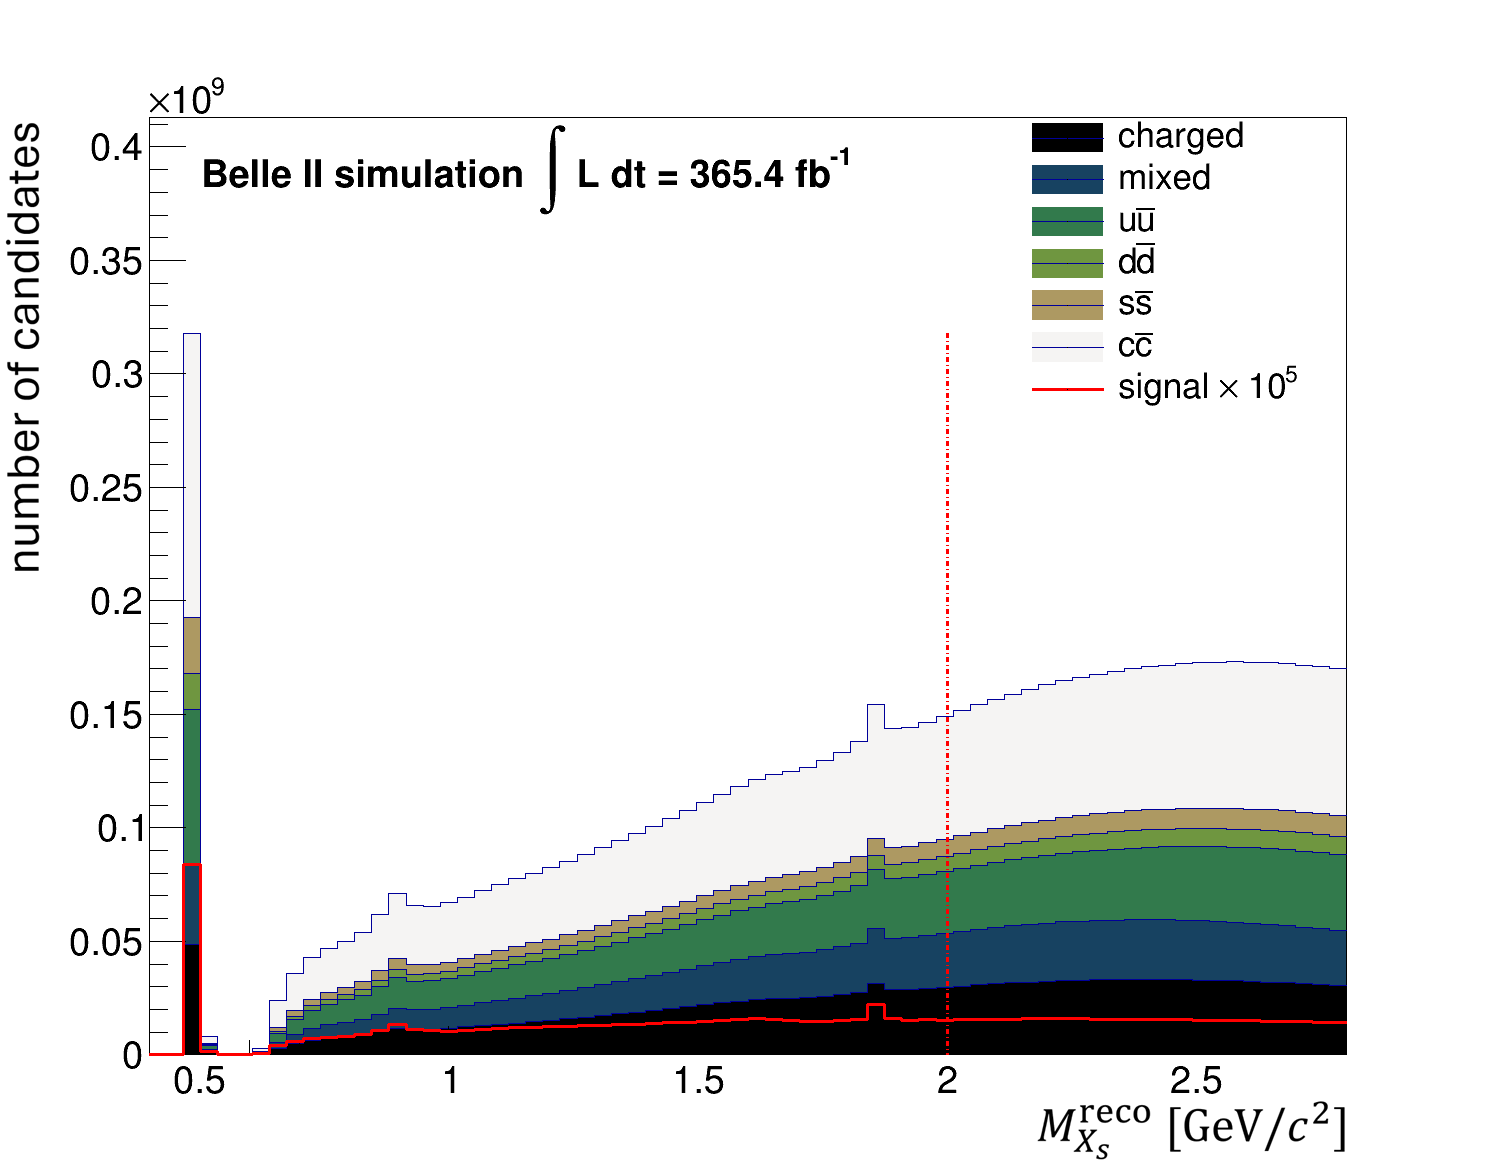
\includegraphics[width=0.65\textwidth]{./picture/Plot_Mxs_preselection.png}
    \caption{$M_{X_{s}}^{\textrm{reco}}$ distribution for the backgrounds and signal MC samples.}
    \label{fig:MXs_preselection}
\end{figure}

Ideally, no tracks, $\pi^0$ candidates, or $K_S^0$ candidates should remain after reconstructing the $\Upsilon(4S)$ candidate.
We require that no $\pi^{0}$ or $K_{S}^{0}$ candidates defined in Section~\ref{sec:particle_selection} remain.
In addition, no loose tracks are allowed to remain.
Loose tracks are defined by $dr < 2~\textrm{cm}$ and $|dz| < 4~\textrm{cm}$.
For these loose tracks, other criteria, such as \texttt{nCDCHits} and \texttt{nPXDHits}, are not applied.

Another preselection criterion is based on vertex-fit information.
In the FEI algorithm, a vertex fit is performed for the $B_{\textrm{tag}}$ candidate.
We require that the vertex fit converge for the $B_{\textrm{tag}}$ candidate.
The decay-chain vertex fit, \texttt{TreeFit}~\cite{Krohn:2019dlq}, is performed for the $X_{s}$ candidates.
This fit is also required to converge for $X_{s}$ whose decay channels have sufficient degrees of freedom for the vertex fit.

Table~\ref{tab:preselection_cutflow} shows the cut flow and the numbers of MC events at the preselection stage.
\begin{sidewaystable}
\caption{
        Number of events surviving the preselection requirements described
        in Section~\ref{sec:preselection}.
        Cross-feed events are included in the signal category.
        The signal and background samples are scaled to an equivalent
        luminosity of $365.37~\textrm{fb}^{-1}$.
        The calibration and correction factors listed in
        Section~\ref{sec:correction} are not applied.
    }
    \centering
    \renewcommand{\arraystretch}{1.25}
    \setlength{\tabcolsep}{5pt}

    \begin{tabularx}{0.98\textheight}{
        >{\raggedright\arraybackslash}X ||
        c | c | c | c | c | c | c
    }
        \hline
        \hline

        \multicolumn{1}{c||}{Selection}
        & SIGNAL
        & CHG
        & MIX
        & UUBAR
        & DDBAR
        & SSBAR
        & CHARM \\
        \hline

        Reconstruction and $M_{X_{s}}^{\textrm{reco}}<2.0~\textrm{GeV}/c^{2}$
        & 206.7
        & $1.47\times10^{7}$
        & $1.01\times10^{7}$
        & $2.34\times10^{7}$
        & $5.41\times10^{6}$
        & $7.44\times10^{6}$
        & $3.86\times10^{7}$ \\

        No remaining $\pi^{0}$
        & 205.3
        & $1.35\times10^{7}$
        & $9.28\times10^{6}$
        & $1.91\times10^{7}$
        & $4.43\times10^{6}$
        & $6.19\times10^{6}$
        & $3.32\times10^{7}$ \\

        No remaining loose tracks
        & 105.2
        & $1.86\times10^{5}$
        & $1.13\times10^{5}$
        & $5.52\times10^{5}$
        & $1.35\times10^{5}$
        & $2.69\times10^{5}$
        & $9.53\times10^{5}$ \\

        No remaining $K_{S}^{0}$
        & 104.9
        & $1.81\times10^{5}$
        & $1.10\times10^{5}$
        & $5.39\times10^{5}$
        & $1.33\times10^{5}$
        & $2.59\times10^{5}$
        & $9.24\times10^{5}$ \\

        $X_{s}$ vertex fit converges
        & 104.9
        & $1.81\times10^{5}$
        & $1.09\times10^{5}$
        & $5.37\times10^{5}$
        & $1.32\times10^{5}$
        & $2.58\times10^{5}$
        & $9.22\times10^{5}$ \\

        $B_{\textrm{tag}}$ vertex fit converges
        & 87.0
        & $1.51\times10^{5}$
        & $8.94\times10^{4}$
        & $4.48\times10^{5}$
        & $1.07\times10^{5}$
        & $2.05\times10^{5}$
        & $6.98\times10^{5}$ \\

        \hline
        \hline
    \end{tabularx}
    \label{tab:preselection_cutflow}
\end{sidewaystable}

\section{Selections}
\label{sec:selection}
After the preselections, several selections are applied to suppress backgrounds, while retaining as much signal as possible.
The selection strategy is to apply loose one-dimensional cut-based selections and a best-candidate selection, followed by a cut on the output of an optimized multivariate analysis~(MVA) classifier.
We use this strategy because optimization at each selection stage does not guarantee global optimization.
Consequently, we try to optimize the selection at the most powerful selection stage, MVA output, and use loose selection criteria before the optimization.

\subsection{One-dimensional cut-based selection}
\label{subsec:one_dimensional_cut}
We require the $B_{\textrm{tag}}$ candidate to satisfy
\begin{equation}
\begin{aligned}
  M_{\textrm{bc}} &> 5.27~\textrm{GeV}/c^{2},\\
  \left| \Delta E \right| &< 0.2~\textrm{GeV}.
\end{aligned}
\end{equation}
Ideally, there should be no remaining energy deposited in the ECL after reconstructing $\Upsilon(4S)$.
The remaining energy deposited in the ECL, $E_{\textrm{ecl}}$, is required to be
\begin{equation}
 E_{\textrm{ecl}} < 1.3~\textrm{GeV}.
\end{equation}
$E_{\textrm{ecl}}$ is defined as the sum of the energies from the ECL clusters which satisfy
\begin{equation}
\begin{cases}
E > 100~\textrm{MeV} &\text{in the forward region}\\
E > 60~\textrm{MeV} &\text{in the barrel region}\\
E > 150~\textrm{MeV} &\text{in the backward region},
\end{cases}
\end{equation}
\begin{equation}
 \texttt{minC2TDist} > 50~\textrm{cm},
\end{equation}
and lie within the CDC acceptance region, where \texttt{minC2TDist} is the distance between the ECL cluster and its nearest track.
These ECL cluster criteria come from the hadronic $B^{+} \rightarrow K^{+} \nu \bar{\nu}$ study~\cite{Belle-II:2023esi}.
Good data-MC agreement is observed for these criteria, according to Figs.~\ref{fig:off_used_vars2} and~\ref{fig:sideband_used_vars2}.

Particles that escape through the beam pipe can mimic missing momentum from neutrinos.
Therefore, the missing momentum is required to satisfy
\begin{equation}
 17^\circ < \theta_{\textrm{missing}} < 150^\circ,
\end{equation}
where $\theta_{\textrm{missing}}$ is the polar angle of the missing momentum in the laboratory frame.
The missing momentum is calculated by the following equation:
\begin{equation}
 \vec{p}_{\textrm{miss}} = \vec{p}_{e^{+}e^{-}} - \sum{\vec{p}_{\textrm{track}}} - \sum{\vec{p}_{\gamma}},
\end{equation}
where $\vec{p}_{\textrm{miss}}$, $\vec{p}_{\textrm{track}}$, and $\vec{p}_{\gamma}$ are the momenta of the $e^{+}e^{-}$ system, tracks, and photons, respectively.
For tracks used to calculate the missing momentum, the following conditions are required:
\begin{itemize}
  \item transverse momentum $p_{t} > 0.1~\textrm{GeV}/c$
  \item within the CDC acceptance region
  \item $dr < 0.5~\textrm{cm}$
  \item $\left| dz \right| < 3~\textrm{cm}$
\end{itemize}
The pion-mass hypothesis is assigned to these tracks.
For photons used to calculate the missing momentum, the following requirements are applied:
\begin{itemize}
  \item $E > 0.05~\textrm{GeV}$
  \item within the CDC acceptance region
  \item $\left| \texttt{clusterTiming} \right| < 200~\textrm{ns}$,
\end{itemize}
where \texttt{clusterTiming} is the difference between the ECL cluster time, obtained from a waveform fit to the highest-energy crystal in the cluster, and the event collision time.
These track and photon requirements are the default options in \texttt{basf2}.

Especially for the low-multiplicity $X_{s}$ decay modes, particles from $B_{\textrm{tag}}$ tend to have lower momenta than the particles forming $X_{s}$.
Therefore, if particles from $B_{\textrm{tag}}$ are used to reconstruct $X_{s}$, the $X_{s}$ momentum becomes lower than that of correctly reconstructed $X_{s}$ candidates.
In addition, $B \rightarrow X_{s} \nu \bar{\nu}$ is a three-body decay and the $X_{s}$ momentum has an upper bound.
We require the momentum of the $X_{s}$ candidates to satisfy
\begin{equation}
  0.5 < p_{X_{s}}^{*} < 2.96~\textrm{GeV}/c
\end{equation}
in the c.m. system.
This requirement is motivated by the $p_{X_{s}}^{*}$ distribution shown in Fig.~\ref{fig:cutvariables} and by the $B \rightarrow h \nu \bar{\nu}$ study.

To remove $D$ mesons that are misidentified as $X_{s}$, a $D$ veto is applied based on the mass of $X_{s}$.
Candidates satisfying
\begin{equation}
  1.84 < M_{X_{s}}^{\textrm{reco}} < 1.89~\textrm{GeV}/c^{2}
\end{equation}
are rejected.
This veto region is determined from the $M_{X_{s}}^{\textrm{reco}}$ distribution shown in Fig.~\ref{fig:cutvariables}.
\begin{figure}
    \centering
    \subfloat{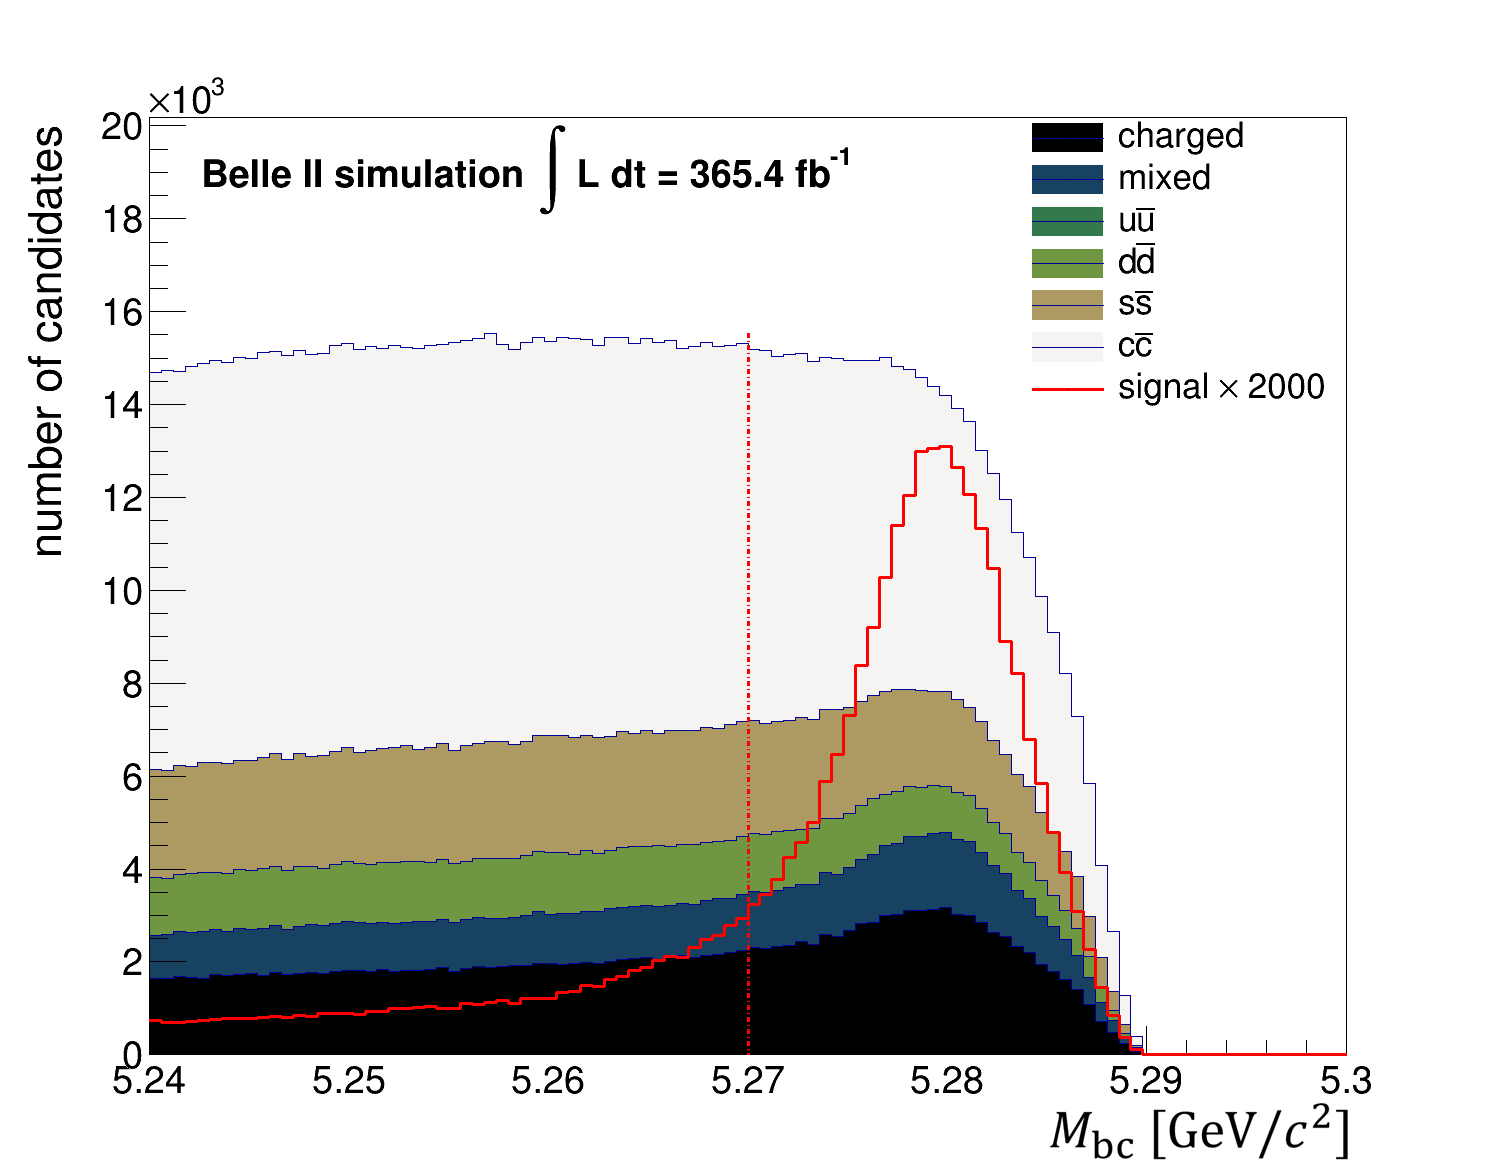
\includegraphics[width=0.45\textwidth]{./picture/Plot_Mbc.png}}
    \subfloat{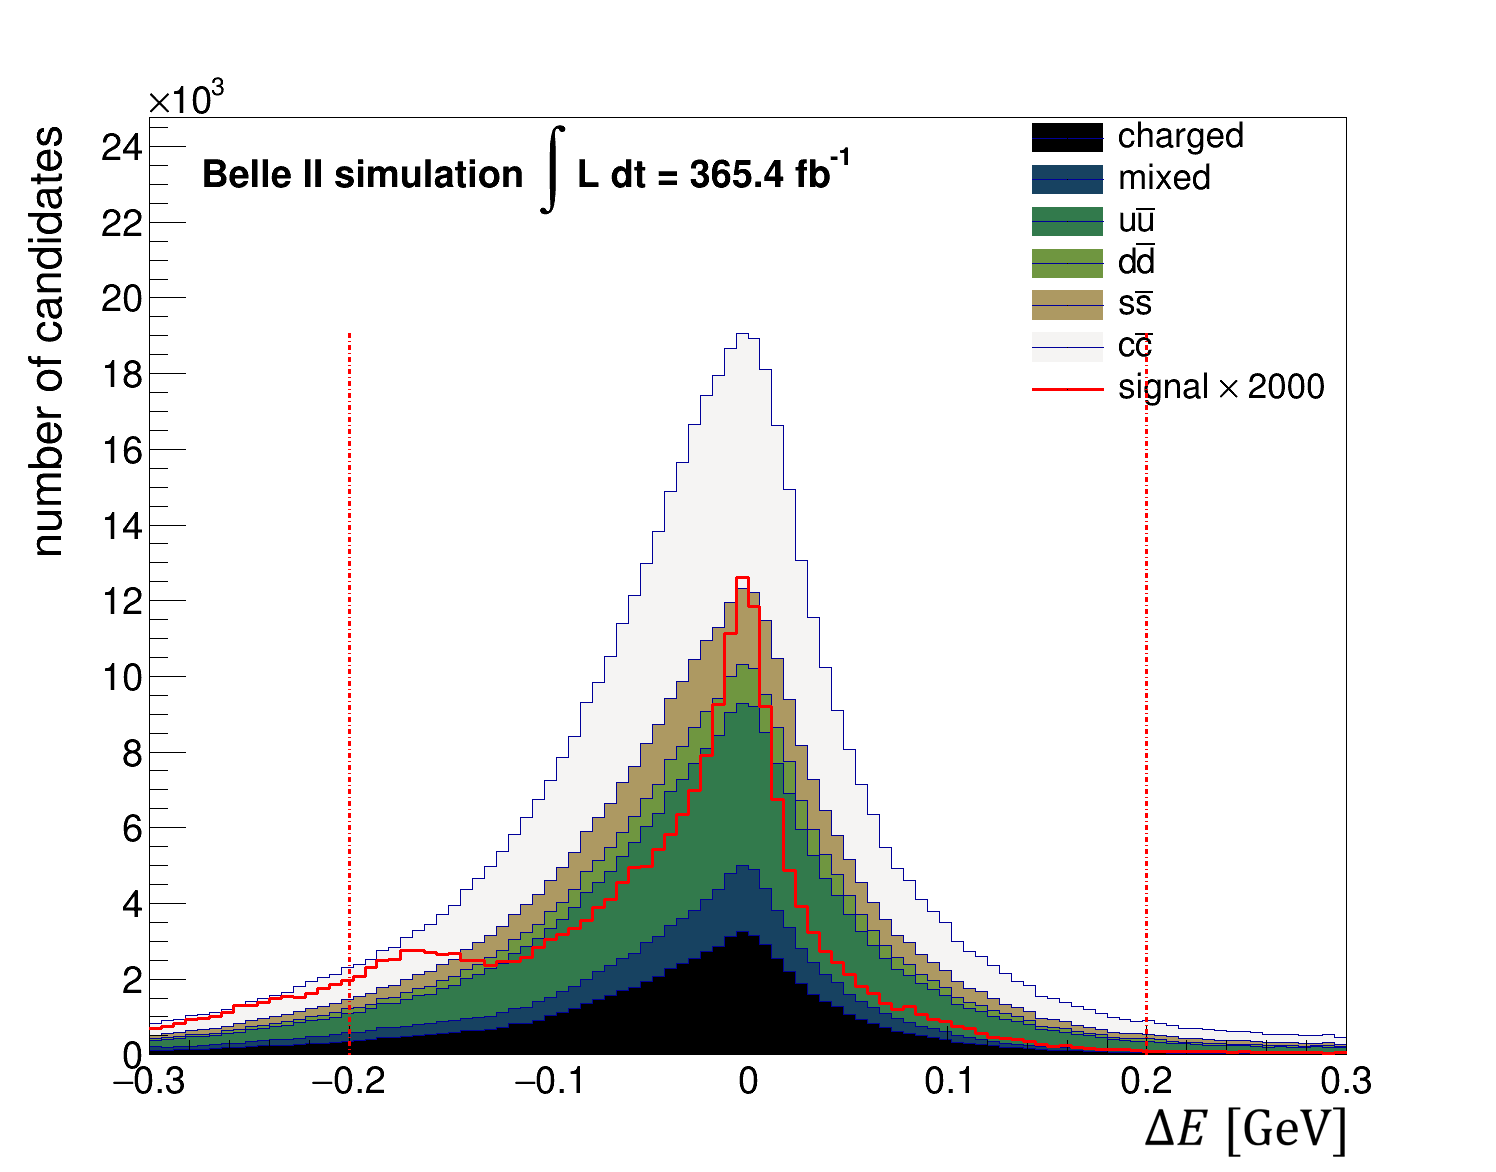
\includegraphics[width=0.45\textwidth]{./picture/Plot_deltaE.png}}\\
    \subfloat{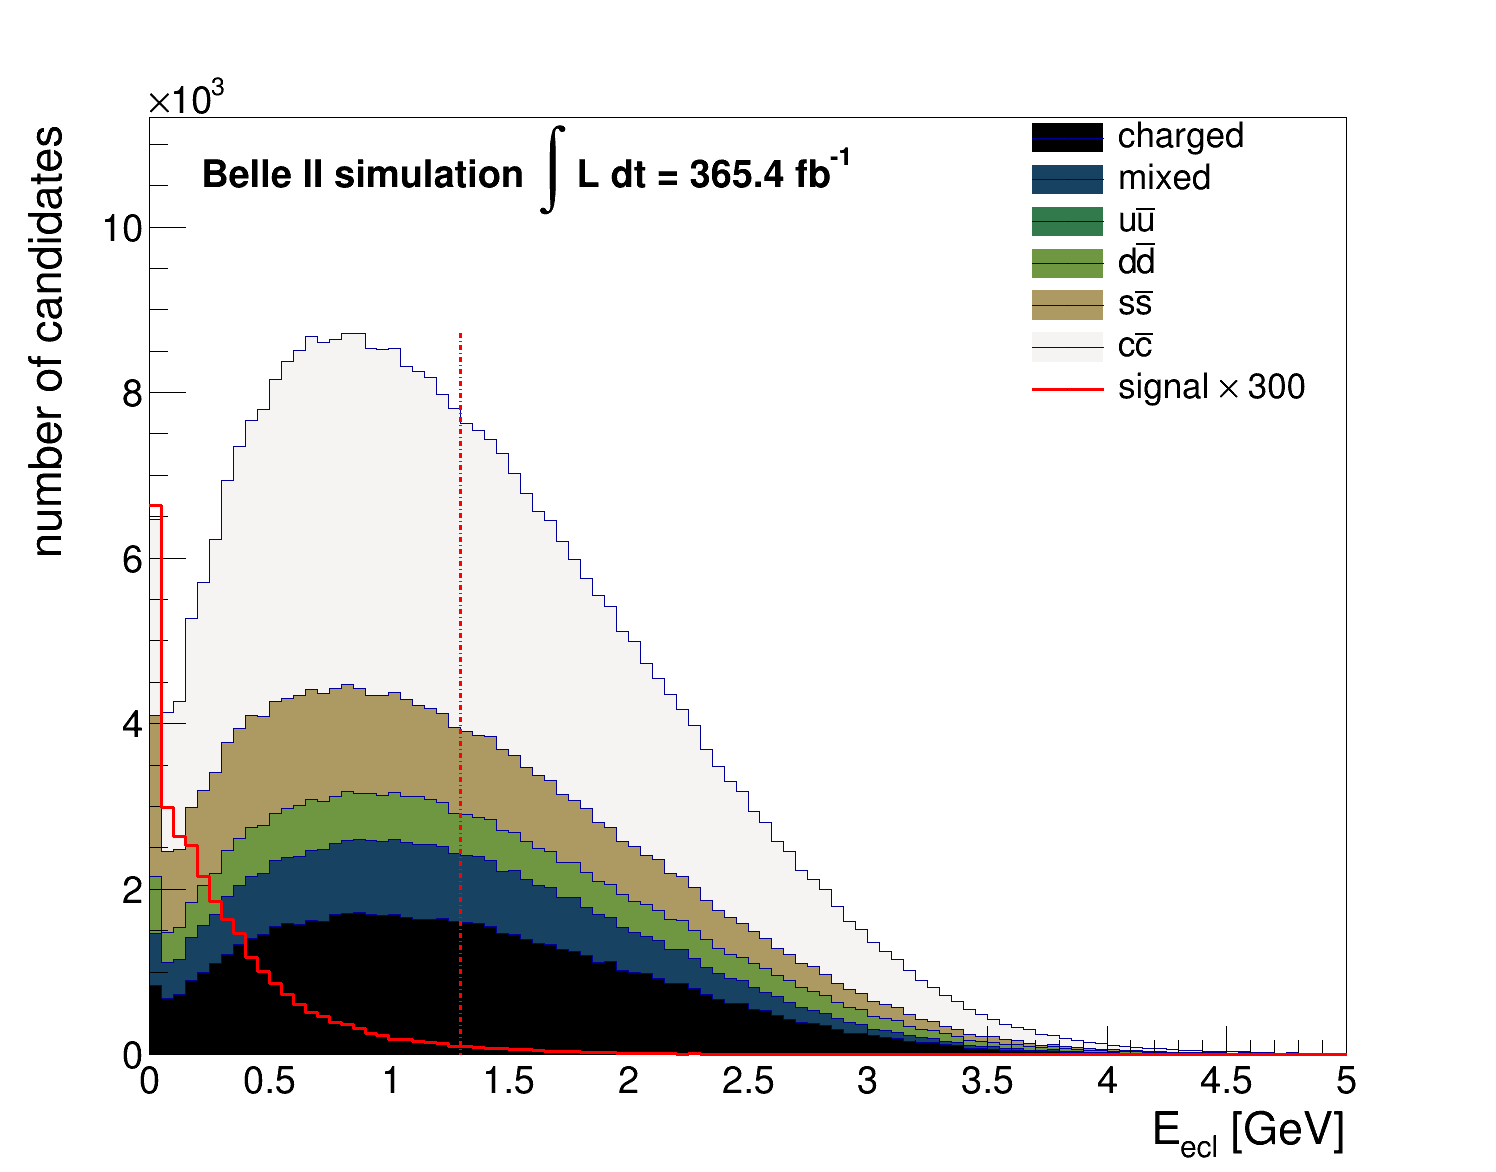
\includegraphics[width=0.45\textwidth]{./picture/Plot_Eecl.png}}
    \subfloat{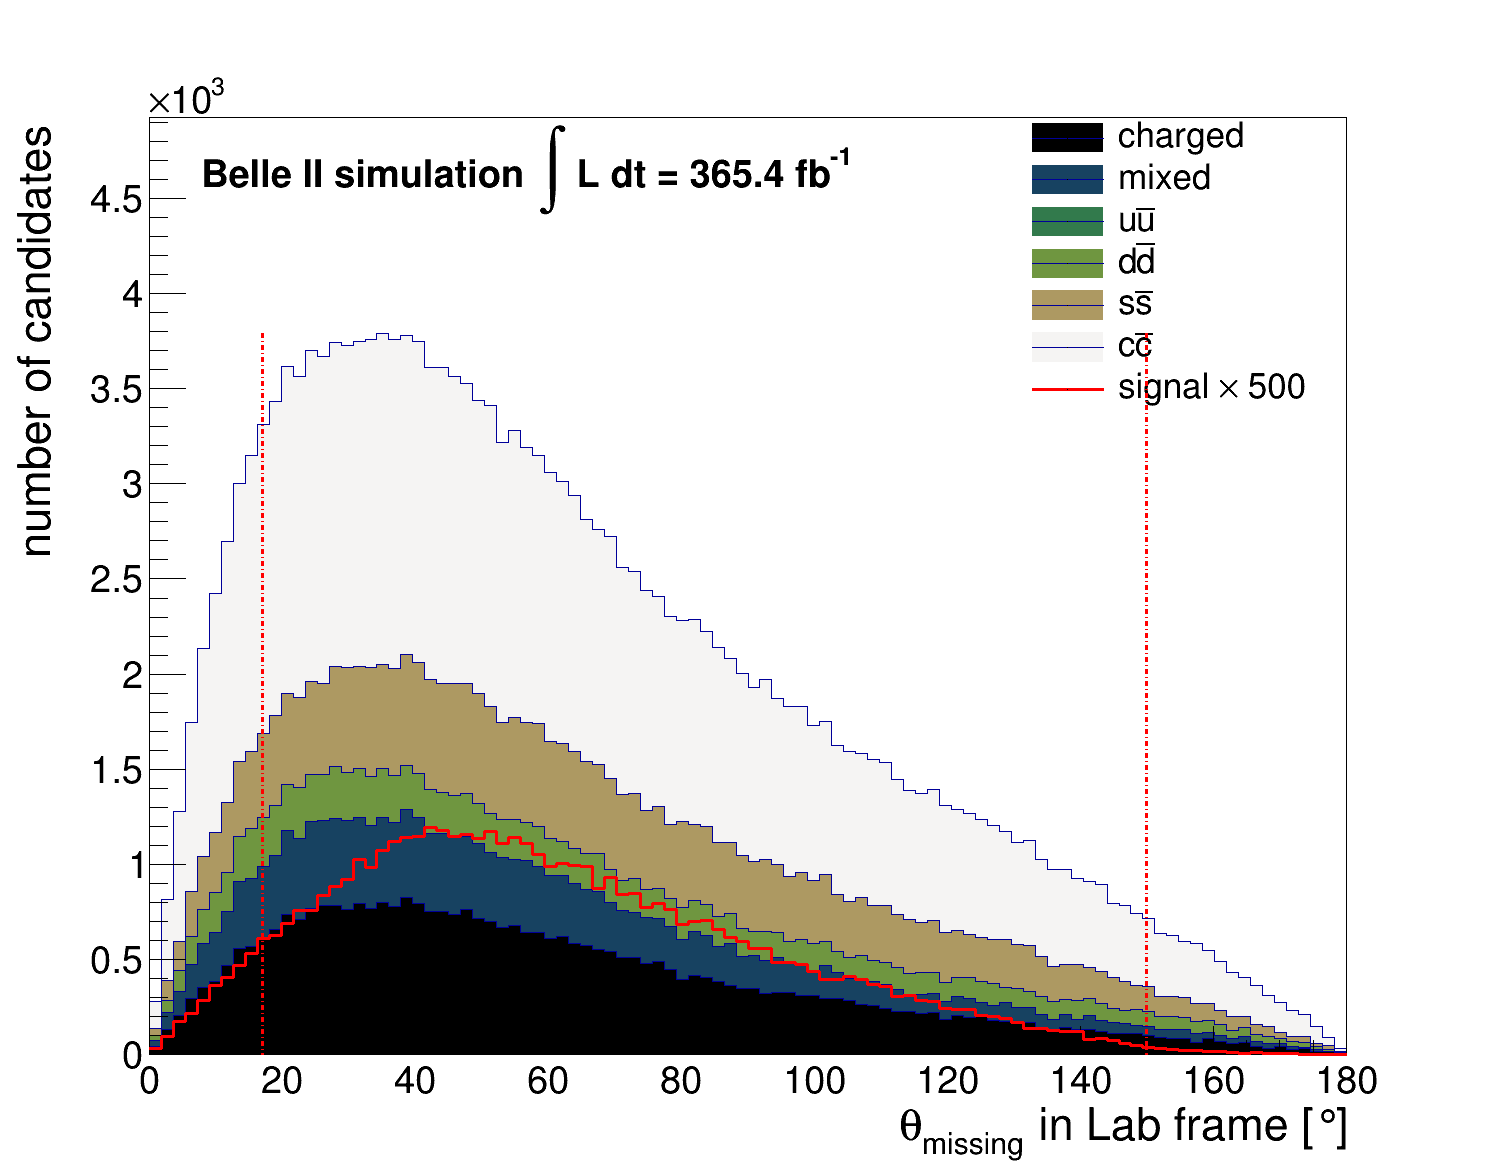
\includegraphics[width=0.45\textwidth]{./picture/Plot_missing_theta_deg.png}}\\
    \subfloat{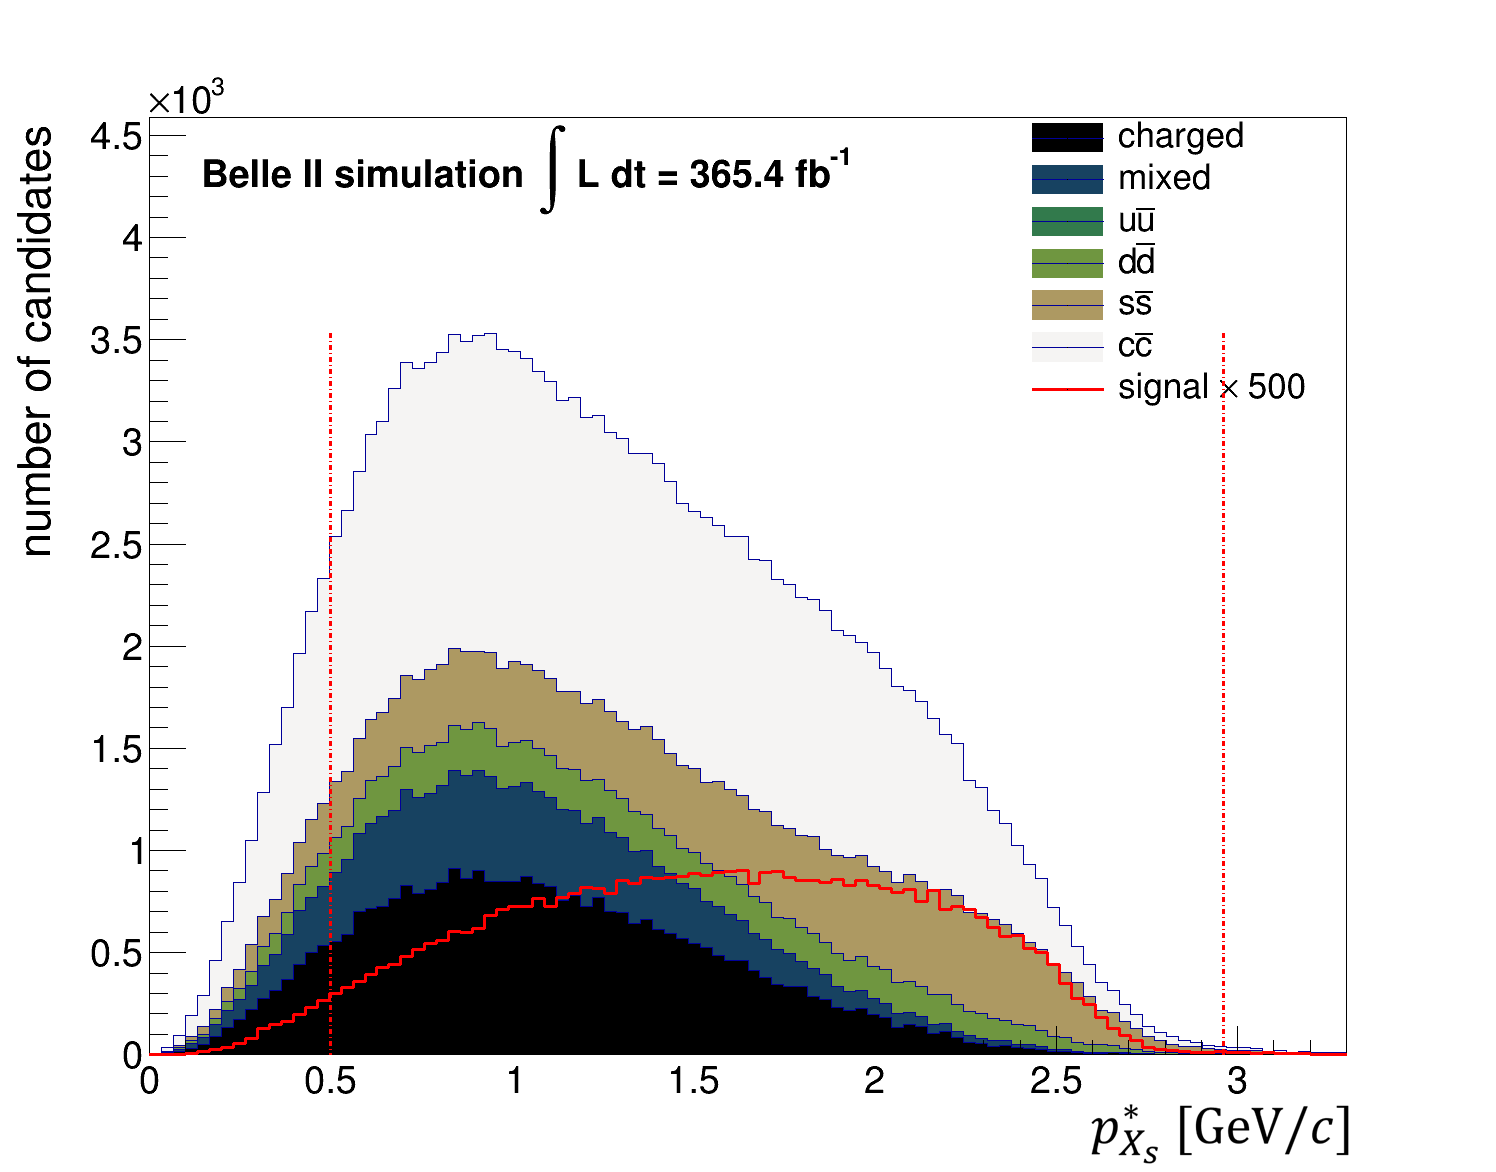
\includegraphics[width=0.45\textwidth]{./picture/Plot_psig.png}}
    \subfloat{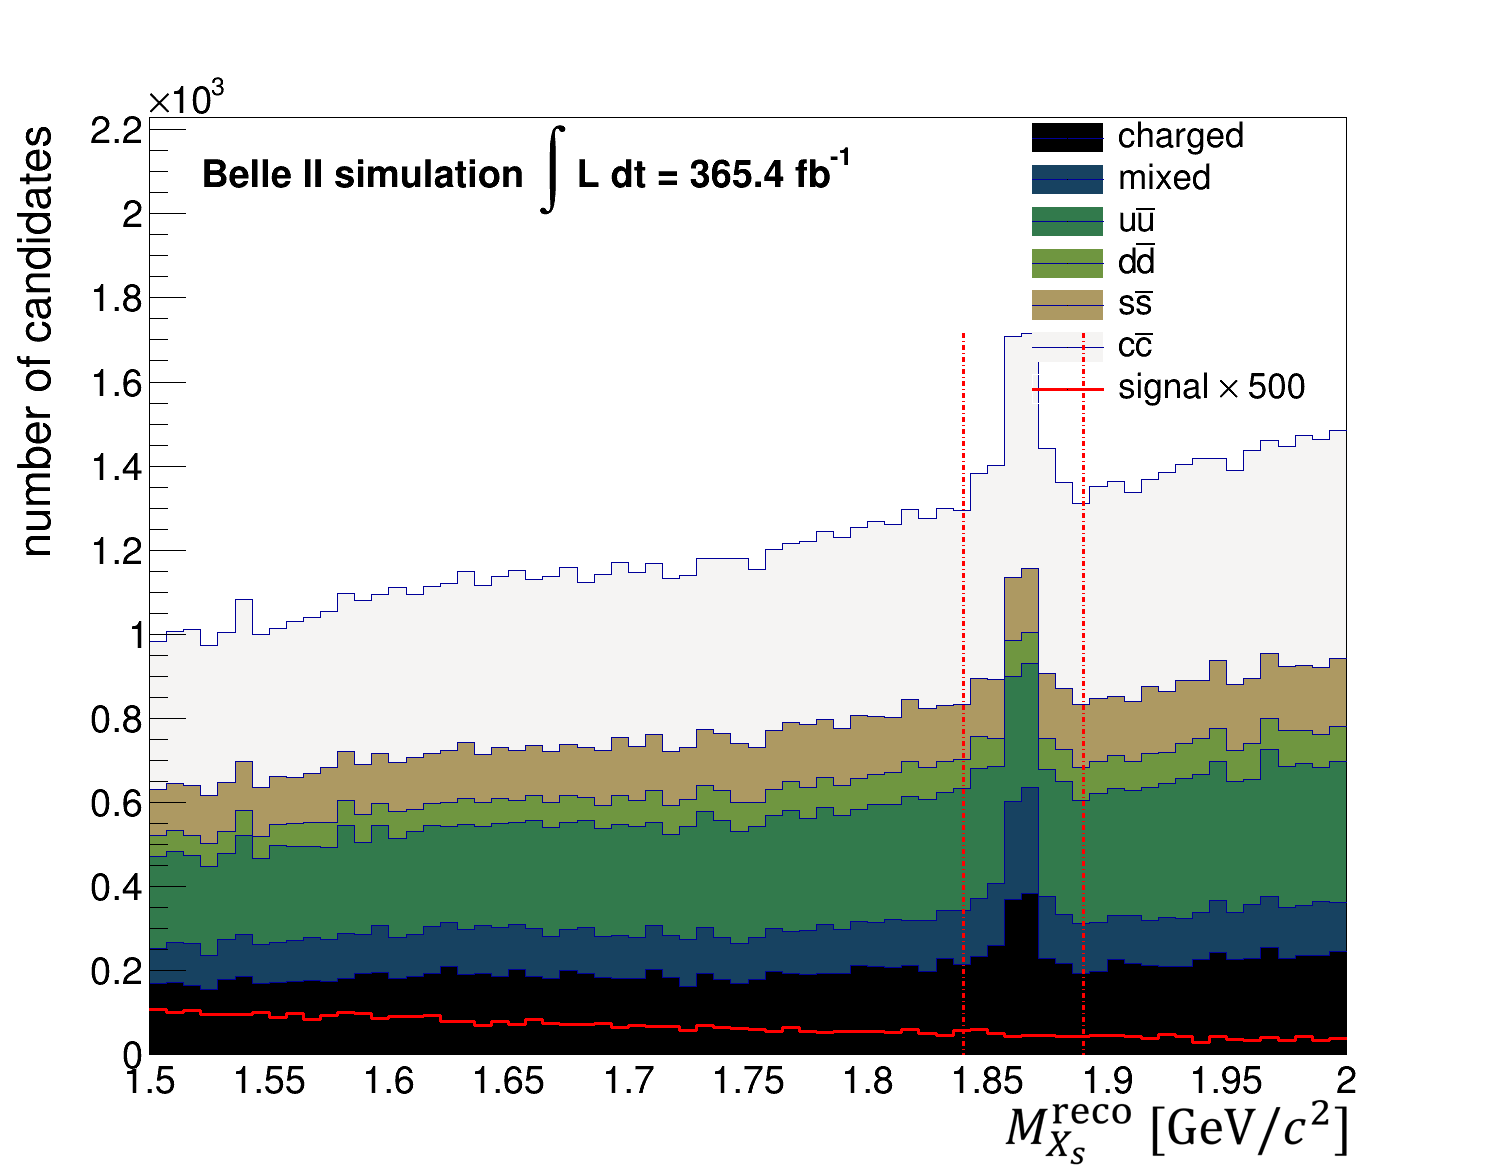
\includegraphics[width=0.45\textwidth]{./picture/Plot_Mxs.png}}
    \caption{Cut variable distributions}
    \label{fig:cutvariables}
\end{figure}

\subsection{Best candidate selection}
After the selections discussed in Section~\ref{subsec:one_dimensional_cut}, the multiplicity of $\Upsilon(4S)$ candidates per event is 1.71 in the signal MC.
Figure~\ref{fig:multiplicity} shows the multiplicity of $\Upsilon(4S)$ candidates for the signal and background MC samples.
The best candidate selection~(BCS) is performed in two steps.
First, we keep the $\Upsilon(4S)$ candidates whose $B_{\textrm{tag}}$ has the highest $\mathcal{P}_{\textrm{FEI}}$ value.
For the signal sample, the fraction of $B_{\textrm{tag}}$ candidates with $\texttt{isSignal} == 1$ increases from 30\% to 46\% after the first step of BCS, where the \texttt{isSignal} value is unity when the particle is correctly reconstructed in \texttt{basf2}.
After the first step of BCS, the multiplicity becomes 1.06 in the signal MC.
There can be more than one $\Upsilon(4S)$ candidate, because there can be exchange between photon candidates in the rest of the event~(ROE) and photon candidates in $\pi^{0}$ used to reconstruct $X_{s}$.
In addition, ROE can have tracks that are not identified as loose tracks defined in Section~\ref{sec:preselection}.
These additional tracks can also be exchanged with tracks in $K^{0}$ candidates used to reconstruct $X_{s}$.
Second, we keep only one $\Upsilon(4S)$ candidate randomly.
The reason why the random selection is used is that other powerful variables will be used in the MVA stage.
\begin{figure}[h]
    \centering
    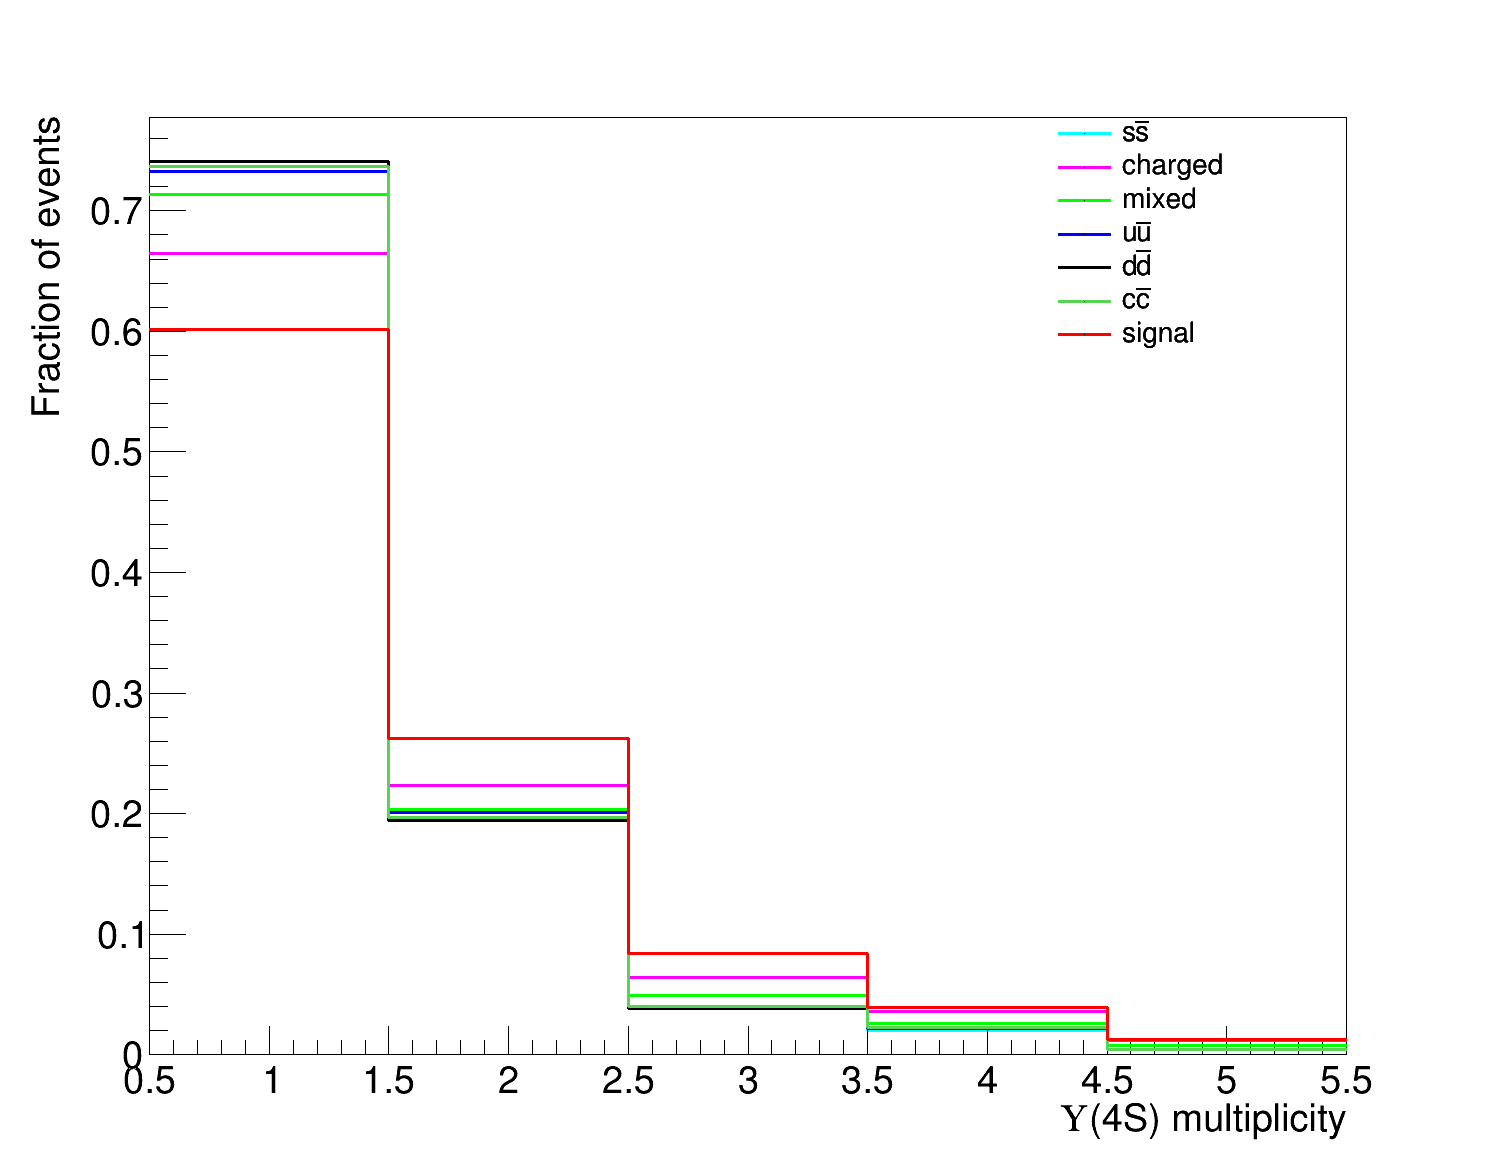
\includegraphics[width=0.65\textwidth]{./picture/Plot_multiplicity.png}
    \caption{The $\Upsilon(4S)$ multiplicity before the best candidate selection stage.}
    \label{fig:multiplicity}
\end{figure}
\subsection{$D$ veto variables}
\label{subsec:Dveto_reconstruction}
Even though $D$ veto is applied, as discussed in Section~\ref{subsec:one_dimensional_cut}, there is still background from $D$ mesons.
To suppress this background, we reconstruct $D$-meson candidates in the event.
Variables derived from these candidates are used as inputs to the MVA classifier described in Section~\ref{subsec:MVA}, together with other variables that discriminate signal from background.
In this section, the reconstruction procedure for these $D$-meson candidates is discussed.

The reconstruction of $D$ mesons is performed using the following procedure:
\begin{enumerate}
  \item \label{item:Kmeson} Select $K^{\pm}$ or $K_{S}^{0}$ candidates from $X_{s}$
  \item \label{item:pimeson} Select $\pi^{\pm}$ candidates from the entire event. Selection criteria are
  \begin{itemize}
    \item $dr < 0.5~\textrm{cm}$, $\left| dz \right| < 2~\textrm{cm}$, and $\texttt{nPXDHits} > 0$
  \end{itemize}
  \item \label{item:pi0meson} Select $\pi^{0}$ candidates from the entire event. The selection criteria are the same as those in Table~\ref{tab:particle_selection}
  \item Reconstruct $D$ meson candidates using the particles selected in steps~\ref{item:Kmeson},~\ref{item:pimeson}, and~\ref{item:pi0meson}. There are four categories of reconstructed decay modes. The first category is
  \begin{itemize}
    \item $D^{+} \rightarrow K_{S}^{0} \pi^{+}$
    \item $D^{+} \rightarrow K^{-} \pi^{+} \pi^{+}$
  \end{itemize}
  The second category is:
  \begin{itemize}
    \item $D^{0} \rightarrow K^{+} \pi^{-}$
    \item $D^{0} \rightarrow K_{S}^{0} \pi^{+} \pi^{-}$
    \item $D^{0} \rightarrow K^{+} \pi^{-} \pi^{+} \pi^{-}$
  \end{itemize}
  The third category is:
  \begin{itemize}
    \item $D^{+} \rightarrow K_{S}^{0} \pi^{+}$
    \item $D^{+} \rightarrow K^{-} \pi^{+} \pi^{+}$
    \item $D^{+} \rightarrow K_{S}^{0} \pi^{+} \pi^{0}$
    \item $D^{+} \rightarrow K^{-} \pi^{+} \pi^{+} \pi^{0}$
    \item $D^{+} \rightarrow K_{S}^{0} \pi^{+} \pi^{0} \pi^{0}$
  \end{itemize}
  The fourth category is:
  \begin{itemize}
    \item $D^{0} \rightarrow K^{+} \pi^{-}$
    \item $D^{0} \rightarrow K_{S}^{0} \pi^{+} \pi^{-}$
    \item $D^{0} \rightarrow K^{+} \pi^{-} \pi^{+} \pi^{-}$
    \item $D^{0} \rightarrow K^{+} \pi^{-} \pi^{0}$
    \item $D^{0} \rightarrow K_{S}^{0} \pi^{+} \pi^{-} \pi^{0}$
    \item $D^{0} \rightarrow K^{+} \pi^{-} \pi^{0} \pi^{0}$
  \end{itemize}
  Including decay modes with $\pi^{0}$ mesons allows us to reconstruct a wider range of $D$ decays, but can also introduce fake $D$ candidates through ECL background.
  Excluding these modes reduces this source of fake candidates, but limits the range of reconstructed $D$ decays.
  We therefore construct both sets of candidates: the first and second categories use only modes without $\pi^{0}$, while the third and fourth categories additionally include modes with $\pi^{0}$.
  Charge-conjugate decay modes are also reconstructed.
  \item Perform a vertex fit. Candidates for which the vertex fit does not converge are not treated as $D$-meson candidates.
\end{enumerate}
In this analysis, the following variables are used as MVA input:
\begin{itemize}
  \item mass of the $D^{\pm}$ candidate with the highest vertex-fit $p$-value in the first category
  \item standard deviation of $p$-value of vertex fitting for $D^{\pm}$ in the first category
  \item mass of the $D^0$ candidate with the highest vertex-fit $p$-value in the second category
  \item standard deviation of $p$-value of vertex fitting for $D^{0}$ in the second category
  \item mass of the $D^{0}$ candidate with the highest vertex-fit $p$-value in the fourth category
  \item standard deviation of $p$-value of vertex fitting for $D^{0}$ in the fourth category
\end{itemize}
As noted above, the third category is not used for MVA.
The reason is that the third category shows some data-MC discrepancy.

\subsection{Multivariate Analysis}
\label{subsec:MVA}
This section discusses the MVA performed after the best-candidate selection.
We use FastBDT as the MVA method~\cite{Keck:2017gsv}.
FastBDT is a boosted-decision-tree-based classifier.
There are some advantages to using FastBDT in the analysis.
First, FastBDT has a shorter training time than deep-learning models or classifiers implemented in the Toolkit for Multivariate Data Analysis~(TMVA).
This shorter training time not only facilitates a smoother analysis workflow but also provides sufficient time for hyperparameter optimization.
Second, for tabular data, tree-based models generally show better performance than deep learning.

To avoid overfitting in FastBDT, we need to constrain the number of input variables.
Two criteria are used to select the input variables of FastBDT: variable importance and data-MC agreement.
The variable importance shows the discriminating power between signal and background samples, which is evaluated using the \texttt{GetVariableRanking()} method provided by FastBDT.
Among powerful variables, we remove the variables that show some data-MC discrepancy in the off-resonance sample and $M_{\textrm{bc}}$ sideband.
Here, the $M_{\textrm{bc}}$ sideband is defined by $M_{\textrm{bc}}<5.26~\textrm{GeV}/c^{2}$ for the $B_{\textrm{tag}}$ candidate.
Figure~\ref{fig:FBDT_var_importance} shows the variable importance for FastBDT input variables.
Appendices~\ref{sec:off_variables}-\ref{sec:side_variables} show distributions of several variables for the off-resonance sample and the sideband region.
A detailed list and descriptions for the input variables are provided in Table~\ref{tab:FastBDT1var}.
Figure~\ref{fig:fewFastBDTinputs} shows two important variables: $E_{\textrm{ecl}}$ and \texttt{harmonicMomentThrust2}.
Figures~\ref{fig:FastBDTinputs1}-\ref{fig:FastBDTinputs2} show the MC distributions of all FastBDT input variables.
\begin{figure}[h]
    \centering
    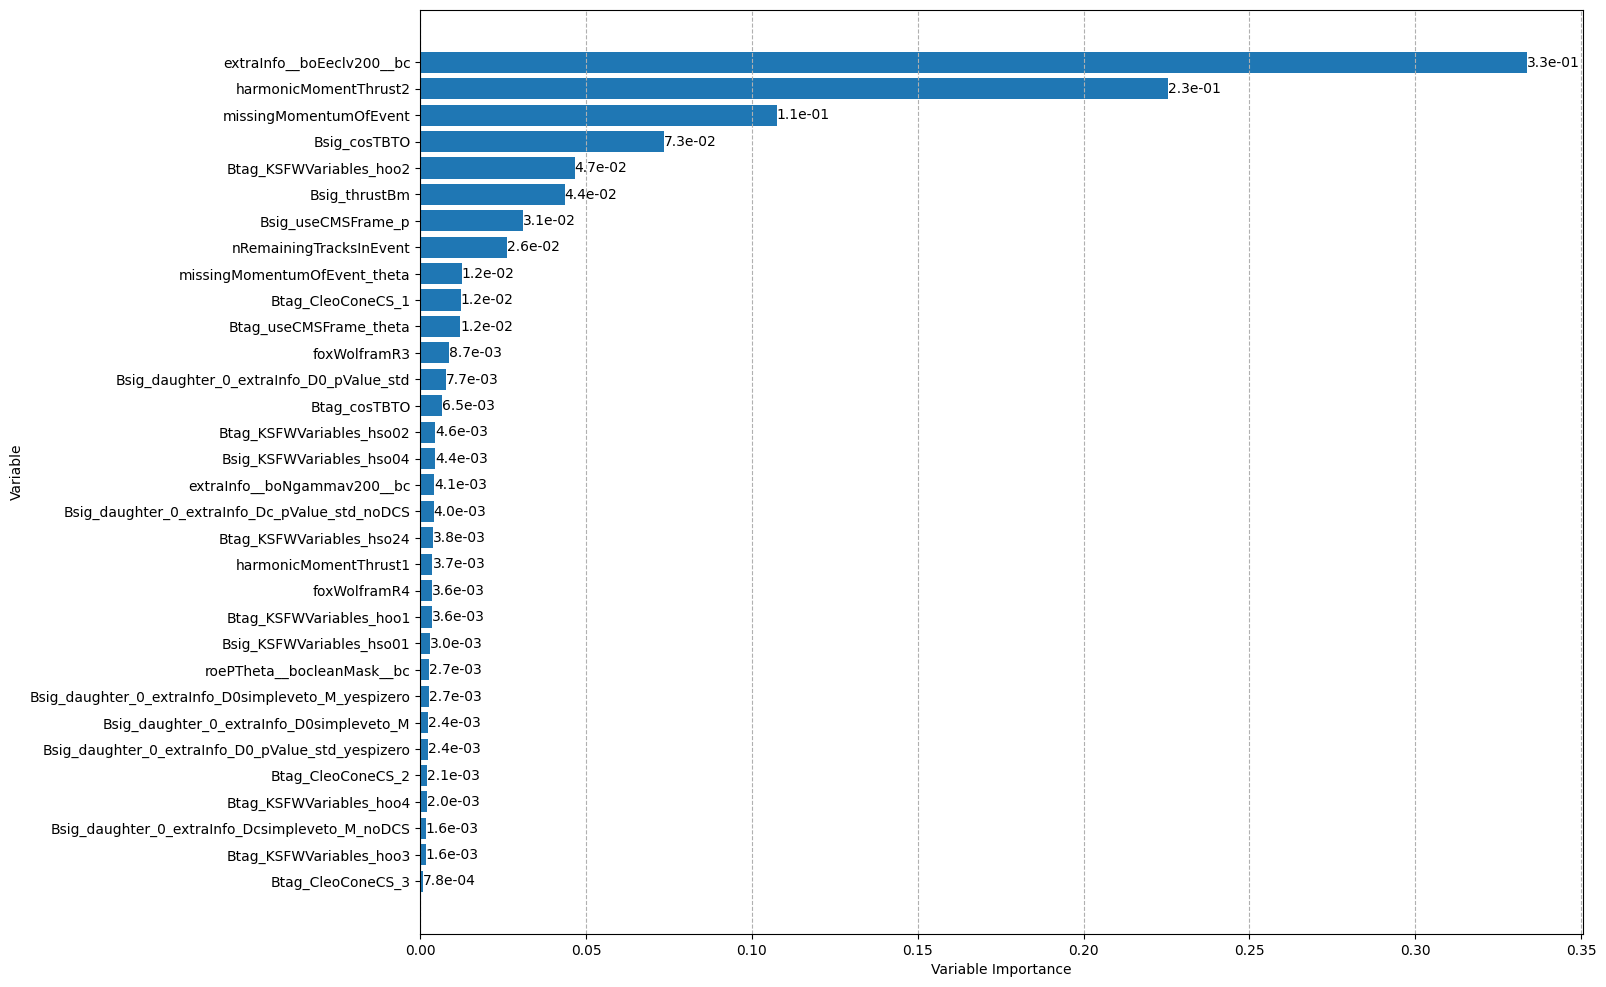
\includegraphics[width=0.95\textwidth]{./picture/FBDT_input/Var_importance.png}
    \caption{Variable importance obtained using the \texttt{GetVariableRanking()} method provided by FastBDT.}
    \label{fig:FBDT_var_importance}
\end{figure}
\begin{figure}[h]
    \centering
    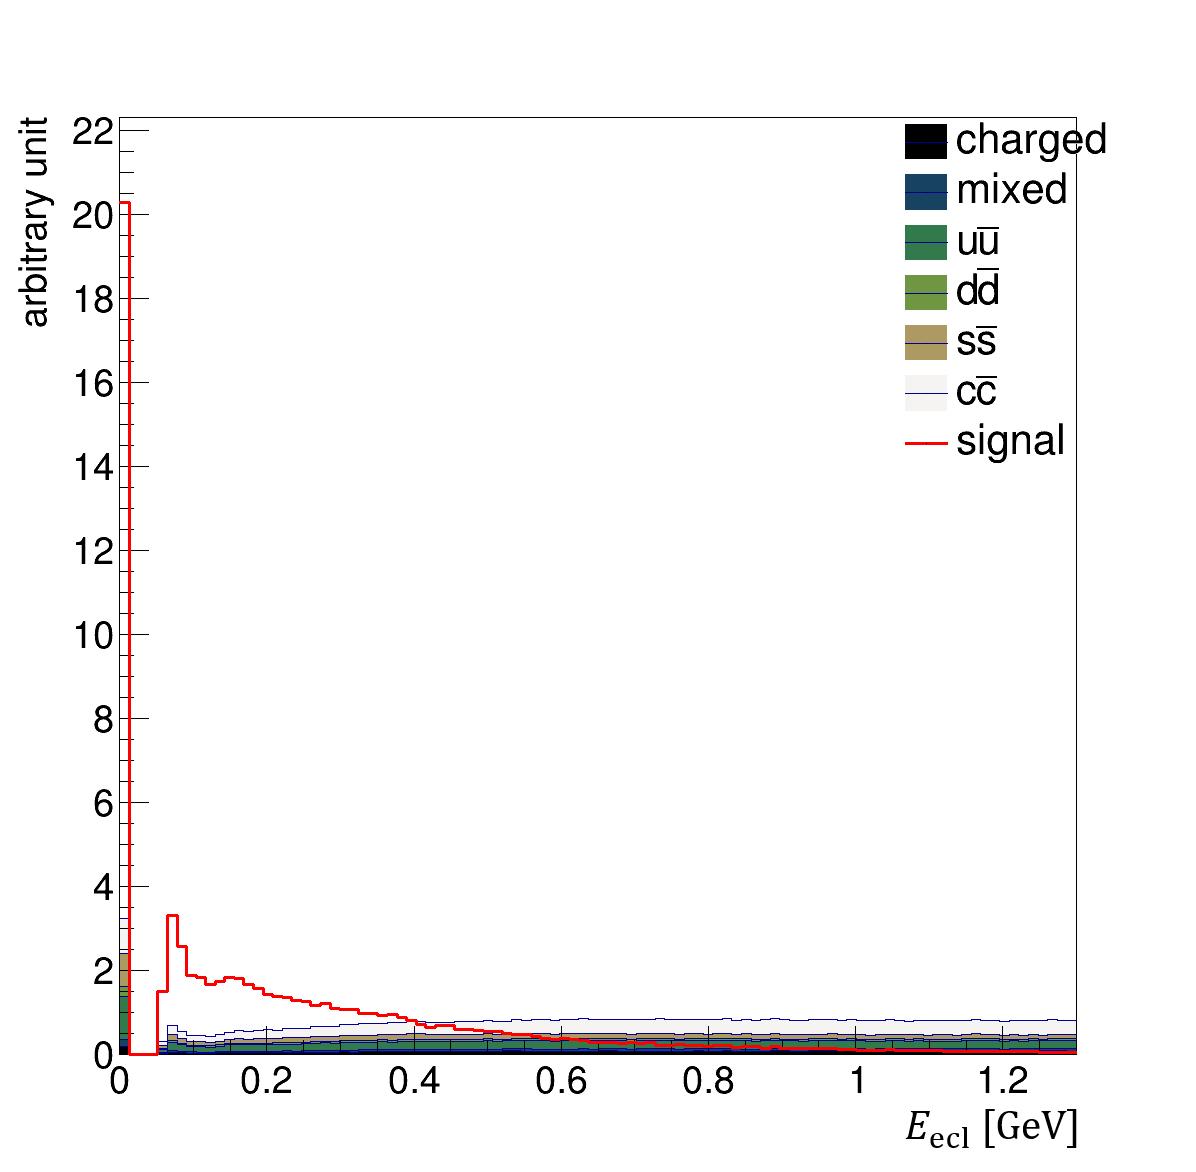
\includegraphics[width=0.48\textwidth]{./picture/FBDT_input/extraInfo__boEeclv200__bc.png}
    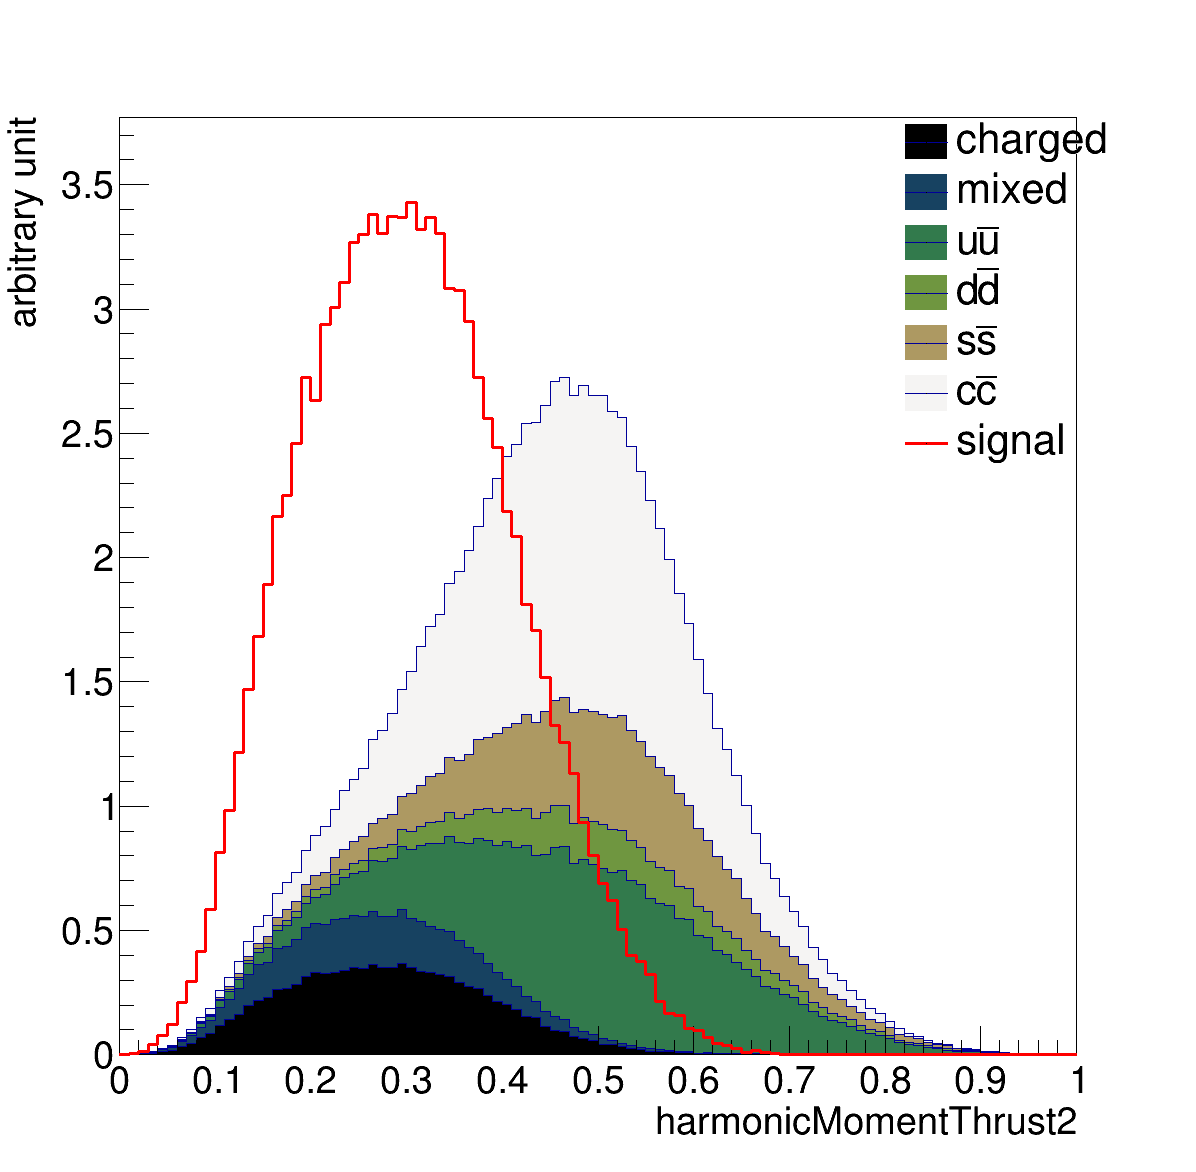
\includegraphics[width=0.48\textwidth]{./picture/FBDT_input/harmonicMomentThrust2.png}
    \caption{Two important FastBDT input variables. The left plot shows the $E_{\textrm{ecl}}$ distribution. The right plot shows \texttt{harmonicMomentThrust2} distribution.}
    \label{fig:fewFastBDTinputs}
\end{figure}

To increase the available training statistics, the MC15ri sample is used to train and test FastBDT. MC15rd sample is used to obtain histogram templates. 
Appendices~\ref{sec:RD_RI_signal_variables}-\ref{sec:RD_RI_background_variables} show the comparison between MC15ri and MC15rd for signal and background samples.

FastBDT has several hyperparameters.
Some of these parameters are optimized by the grid search method.
Table~\ref{tab:FBDT_gridsearch} shows the names of the hyperparameters and their descriptions, tested values in the grid search, and the selected value.
\begin{table}
\caption{Name of hyperparameters, descriptions, and their values.}
  \renewcommand{\arraystretch}{1.2}
  \centering

  \resizebox{\textwidth}{!}{%
    \begin{tabular}{p{2cm}|p{4.5cm}|p{6cm}|p{3cm}}
      \hline
      \hline
      \multicolumn{1}{c|}{Name}
      & \multicolumn{1}{c|}{Description}
      & \multicolumn{1}{c|}{Tested values}
      & \multicolumn{1}{c}{Selected value} \\
      \hline

      \multicolumn{1}{c|}{\texttt{nTrees}}
      & Number of trees
      & \multicolumn{1}{c|}{100, 500, 1000, 1500, 2000}
      & \multicolumn{1}{c}{2000} \\

      \multicolumn{1}{c|}{\texttt{depth}}
      & Maximum tree depth
      & \multicolumn{1}{c|}{2, 3, 4}
      & \multicolumn{1}{c}{3} \\

      \multicolumn{1}{c|}{\texttt{shrinkage}}
      & Learning rate
      & \multicolumn{1}{c|}{0.05, 0.1, 0.15, 0.2}
      & \multicolumn{1}{c}{0.05} \\

      \multicolumn{1}{c|}{\texttt{subsample}}
      & Sampling fraction
      & \multicolumn{1}{c|}{0.3, 0.4, 0.5, 0.6, 0.7}
      & \multicolumn{1}{c}{0.5} \\

      \multicolumn{1}{c|}{\texttt{binning}}
      & Number of binning levels
      & \multicolumn{1}{c|}{6, 7, 8, 9}
      & \multicolumn{1}{c}{6} \\

      \hline
      \hline
    \end{tabular}%
  }
  \label{tab:FBDT_gridsearch}
\end{table}
In the grid search, the AUC is used as the optimization criterion.
Figure~\ref{fig:gridsearch} shows the result of the grid search.
For each hyperparameter combination in the grid search, there are two AUC values: AUC from training and testing samples.
We want to keep the AUC value as large as possible, while keeping the testing AUC close to the training AUC.
The x-axis of the figure is the rank of the AUC value for the testing sample.
A lower rank indicates a higher AUC value.
The blue dots show the AUC values for the testing sample.
The red dots show the AUC values for the training sample.
\begin{figure}[h]
    \centering
    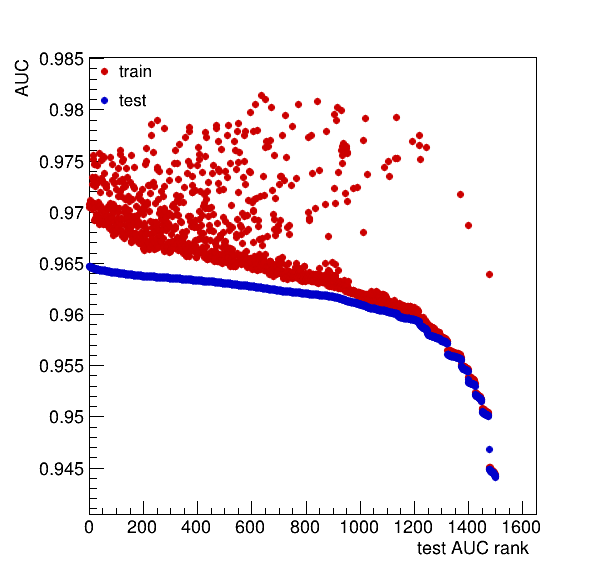
\includegraphics[width=0.65\textwidth]{./picture/FBDT_input/AUC.png}
    \caption{Result of grid search. $x$-axis shows rank of AUC value for the testing sample. Lower rank means higher AUC value. $y$-axis shows AUC value. The blue dots show the AUC values for the testing sample. The red dots show the AUC values for the training sample.}
    \label{fig:gridsearch}
\end{figure}
With the selected hyperparameters in Table~\ref{tab:FBDT_gridsearch}, the AUC values for training and testing samples are 0.966473 and 0.963756, respectively.
The difference in the AUC value is smaller than 0.3\%.
Therefore, we conclude that the overfitting is negligible.

Figure~\ref{fig:FastBDToutputs} shows the FastBDT output distribution for the training signal MC, testing signal MC, training background MC, and testing background MC samples.
\begin{figure}[h]
    \centering
    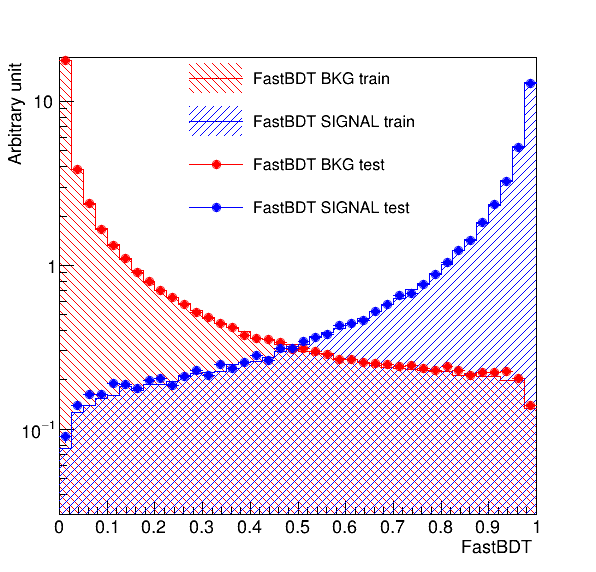
\includegraphics[width=0.65\textwidth]{./picture/FBDT_output/OBB_Plot.png}
    \caption{FastBDT output distribution.}
    \label{fig:FastBDToutputs}
\end{figure}

The cut criterion on the FastBDT output is determined by the figure of merit~(FOM):
\begin{equation}
    \textrm{FOM} = \frac{S}{\sqrt{S+B}},
\end{equation}
where $S$ and $B$ are the numbers of signal and background events, respectively.
Figure~\ref{fig:FOMplot} shows the FOM value as a function of the FastBDT cut.
\begin{figure}
\centering
\subfloat[][$0.0 < M_{X_{s}}^{\textrm{reco}} < 0.6~\textrm{GeV}/c^2$]{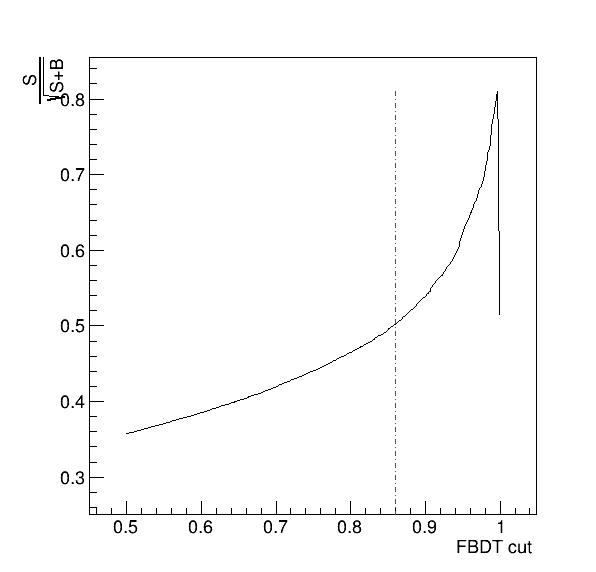
\includegraphics[width=0.32\textwidth]{./picture/FBDT_output/FOM_K.png}}
\subfloat[][$0.6 \leq M_{X_{s}}^{\textrm{reco}} < 1.0~\textrm{GeV}/c^2$]{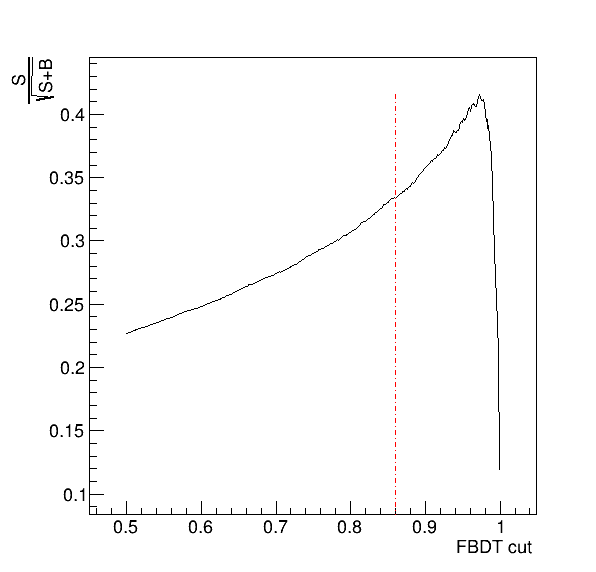
\includegraphics[width=0.32\textwidth]{./picture/FBDT_output/FOM_Kstar.png}}
\subfloat[][$1.0 \leq M_{X_{s}}^{\textrm{reco}} < 2.0~\textrm{GeV}/c^2$]{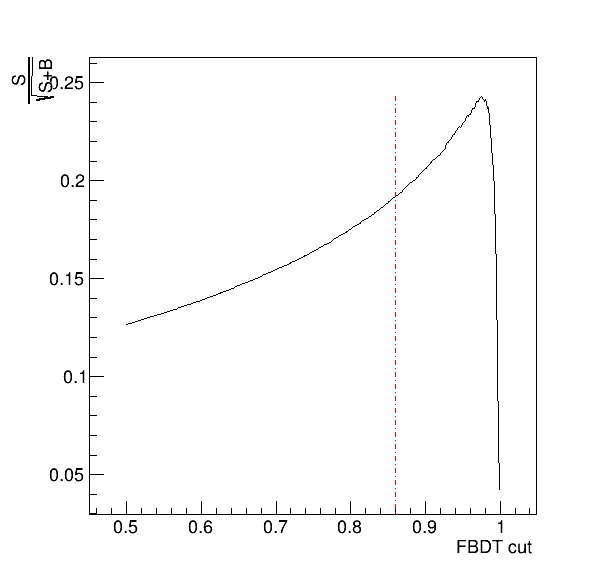
\includegraphics[width=0.32\textwidth]{./picture/FBDT_output/FOM_Xs.png}}
\caption{FOM distribution for (a)~$0.0 < M_{X_{s}}^{\textrm{reco}} < 0.6~\textrm{GeV}/c^2$, (b)~$0.6 \leq M_{X_{s}}^{\textrm{reco}} < 1.0~\textrm{GeV}/c^2$, and (c)~$1.0 \leq M_{X_{s}}^{\textrm{reco}} < 2.0~\textrm{GeV}/c^2$. The FOMs are maximized near $\textrm{FBDT}>0.996$, $\textrm{FBDT}>0.973$, and $\textrm{FBDT}>0.975$, respectively.}
\label{fig:FOMplot}
\end{figure}
The signal yield extraction will be performed using the FastBDT output variable.
Consequently, we do not apply the FastBDT cut which maximizes FOM values.
Instead, we apply a loose requirement on the FastBDT output,
$\mathcal{O}_{\textrm{BDT}} > 0.86$, and use the signal-depleted region to estimate the background yields.

\section{Summary}
Table~\ref{tab:cutflow} shows the cut flow described in Section~\ref{sec:selection}.
The signal and background samples are scaled to an equivalent integrated luminosity of $365.37~\textrm{fb}^{-1}$.
\begin{sidewaystable}
\caption{
        Numbers of events surviving the selection requirements described
        in Section~\ref{sec:selection}.
        The signal and background samples are scaled to an equivalent
        integrated luminosity of $365.37~\textrm{fb}^{-1}$.
        Cross-feed events are included in the signal category.
        The calibration and correction factors listed in
        Section~\ref{sec:correction} are not applied.
    }
    \centering
    \renewcommand{\arraystretch}{1.2}
    \setlength{\tabcolsep}{5pt}
    \small

    \begin{tabularx}{0.95\textheight}{
        >{\raggedright\arraybackslash}X ||
        c | c | c | c | c | c | c
    }
        \hline
        \hline

        \multicolumn{1}{c||}{Selection}
        & SIGNAL
        & CHG
        & MIX
        & UUBAR
        & DDBAR
        & SSBAR
        & CHARM \\
        \hline

        Generated
        & 22451.8
        & \multicolumn{6}{c}{$365.37~\textrm{fb}^{-1}$} \\

        Skim
        & 689.1
        & $3.44\times10^{7}$
        & $2.62\times10^{7}$
        & $9.11\times10^{7}$
        & $2.19\times10^{7}$
        & $1.73\times10^{7}$
        & $9.64\times10^{7}$ \\

        Reconstruction and preselections
        & 86.8
        & $1.51\times10^{5}$
        & $8.94\times10^{4}$
        & $4.48\times10^{5}$
        & $1.07\times10^{5}$
        & $2.05\times10^{5}$
        & $6.98\times10^{5}$ \\

        $M_{\textrm{bc}} > 5.27~\textrm{GeV}/c^{2}$ for $B_{\textrm{tag}}$
        & 61.4
        & 40488.1
        & 23369.8
        & 83729.7
        & 20103.7
        & 39879.0
        & $1.24\times10^{5}$ \\

        $\left|\Delta E\right| < 0.2~\textrm{GeV}$ for $B_{\textrm{tag}}$
        & 57.6
        & 39106.5
        & 22283.9
        & 78875.1
        & 18935.4
        & 37449.6
        & $1.17\times10^{5}$ \\

        $E_{\textrm{ecl}} < 1.3~\textrm{GeV}$
        & 56.1
        & 21913.3
        & 12983.9
        & 41440.5
        & 9974.0
        & 22868.4
        & 64568.4 \\

        $17^\circ < \theta_{\textrm{missing}} < 150^\circ$
        & 52.5
        & 19354.9
        & 11321.3
        & 34360.5
        & 8337.9
        & 20314.0
        & 55395.6 \\

        $0.5 < p_{X_{s}}^{*} < 2.96~\textrm{GeV}/c$
        & 50.8
        & 17532.5
        & 10174.3
        & 31450.0
        & 7658.2
        & 19136.3
        & 50693.7 \\

        Reject $1.84 < M_{X_{s}}^{\textrm{reco}} < 1.89~\textrm{GeV}/c^{2}$
        & 50.6
        & 16452.4
        & 9521.7
        & 30161.8
        & 7350.9
        & 18498.2
        & 48501.4 \\

        BCS
        & 50.6
        & 16452.4
        & 9521.7
        & 30161.8
        & 7350.9
        & 18498.2
        & 48501.4 \\

        $\mathcal{O}_{\textrm{BDT}} > 0.86$
        & 34.5
        & 1604.3
        & 796.4
        & 471.6
        & 113.9
        & 475.8
        & 641.6 \\

        \hline
        \hline
    \end{tabularx}
    \label{tab:cutflow}
\end{sidewaystable}
The efficiency as a function of $M_{X_{s}}$ is shown in Section~\ref{sec:efficiency_as_MXs}.
Figure~\ref{fig:Diagonal_Efficiencymatrix} shows the proper reconstruction efficiency for each $X_{s}$ decay mode.
Figure~\ref{fig:crossfeedmatrix} shows the cross-feed matrix.
The cross-feed matrix is defined as $\epsilon_{\mathrm{mode}}/\epsilon_{\mathrm{true}}$, where $\epsilon_{\mathrm{mode}}$ is the efficiency for events to be reconstructed in a given mode, and $\epsilon_{\mathrm{true}}$ is the efficiency for events to be reconstructed in the correct decay mode.

\begin{figure}
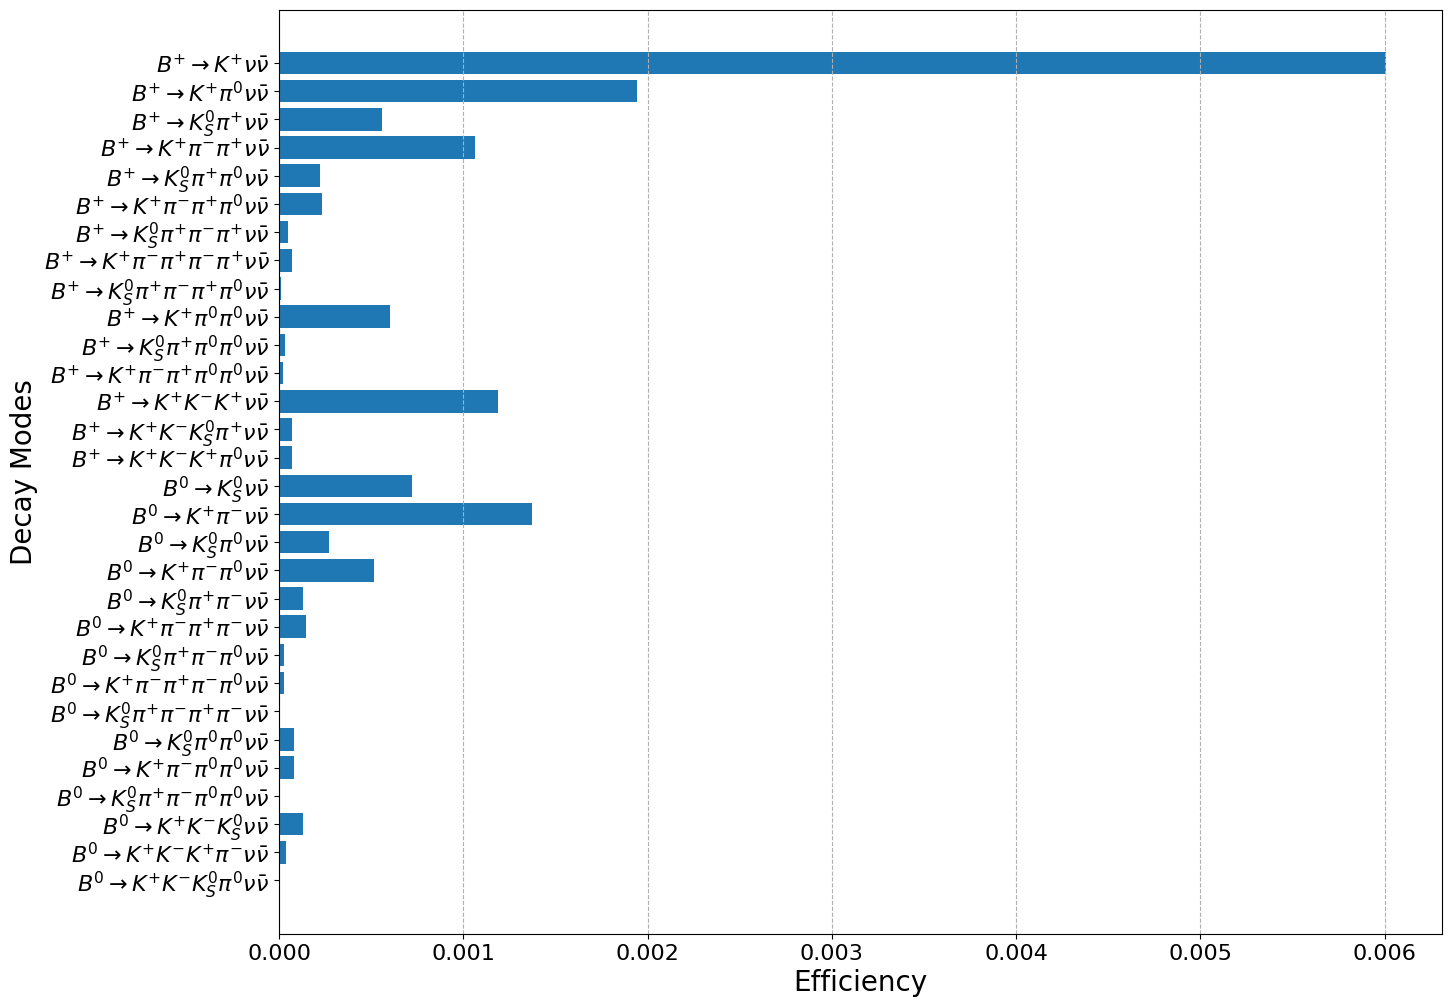
\includegraphics[width=0.9\textwidth]{./picture/Diagonal_Efficiency.png}
\caption{Proper reconstruction efficiencies after all selection requirements are applied. For example, the efficiency for $B^{+}\rightarrow K^{+}\nu\bar{\nu}$ events to be reconstructed as $B^{+}\rightarrow K^{+}\nu\bar{\nu}$ is $6.01\times 10^{-3}$.}
\label{fig:Diagonal_Efficiencymatrix}
\end{figure}
\begin{figure}
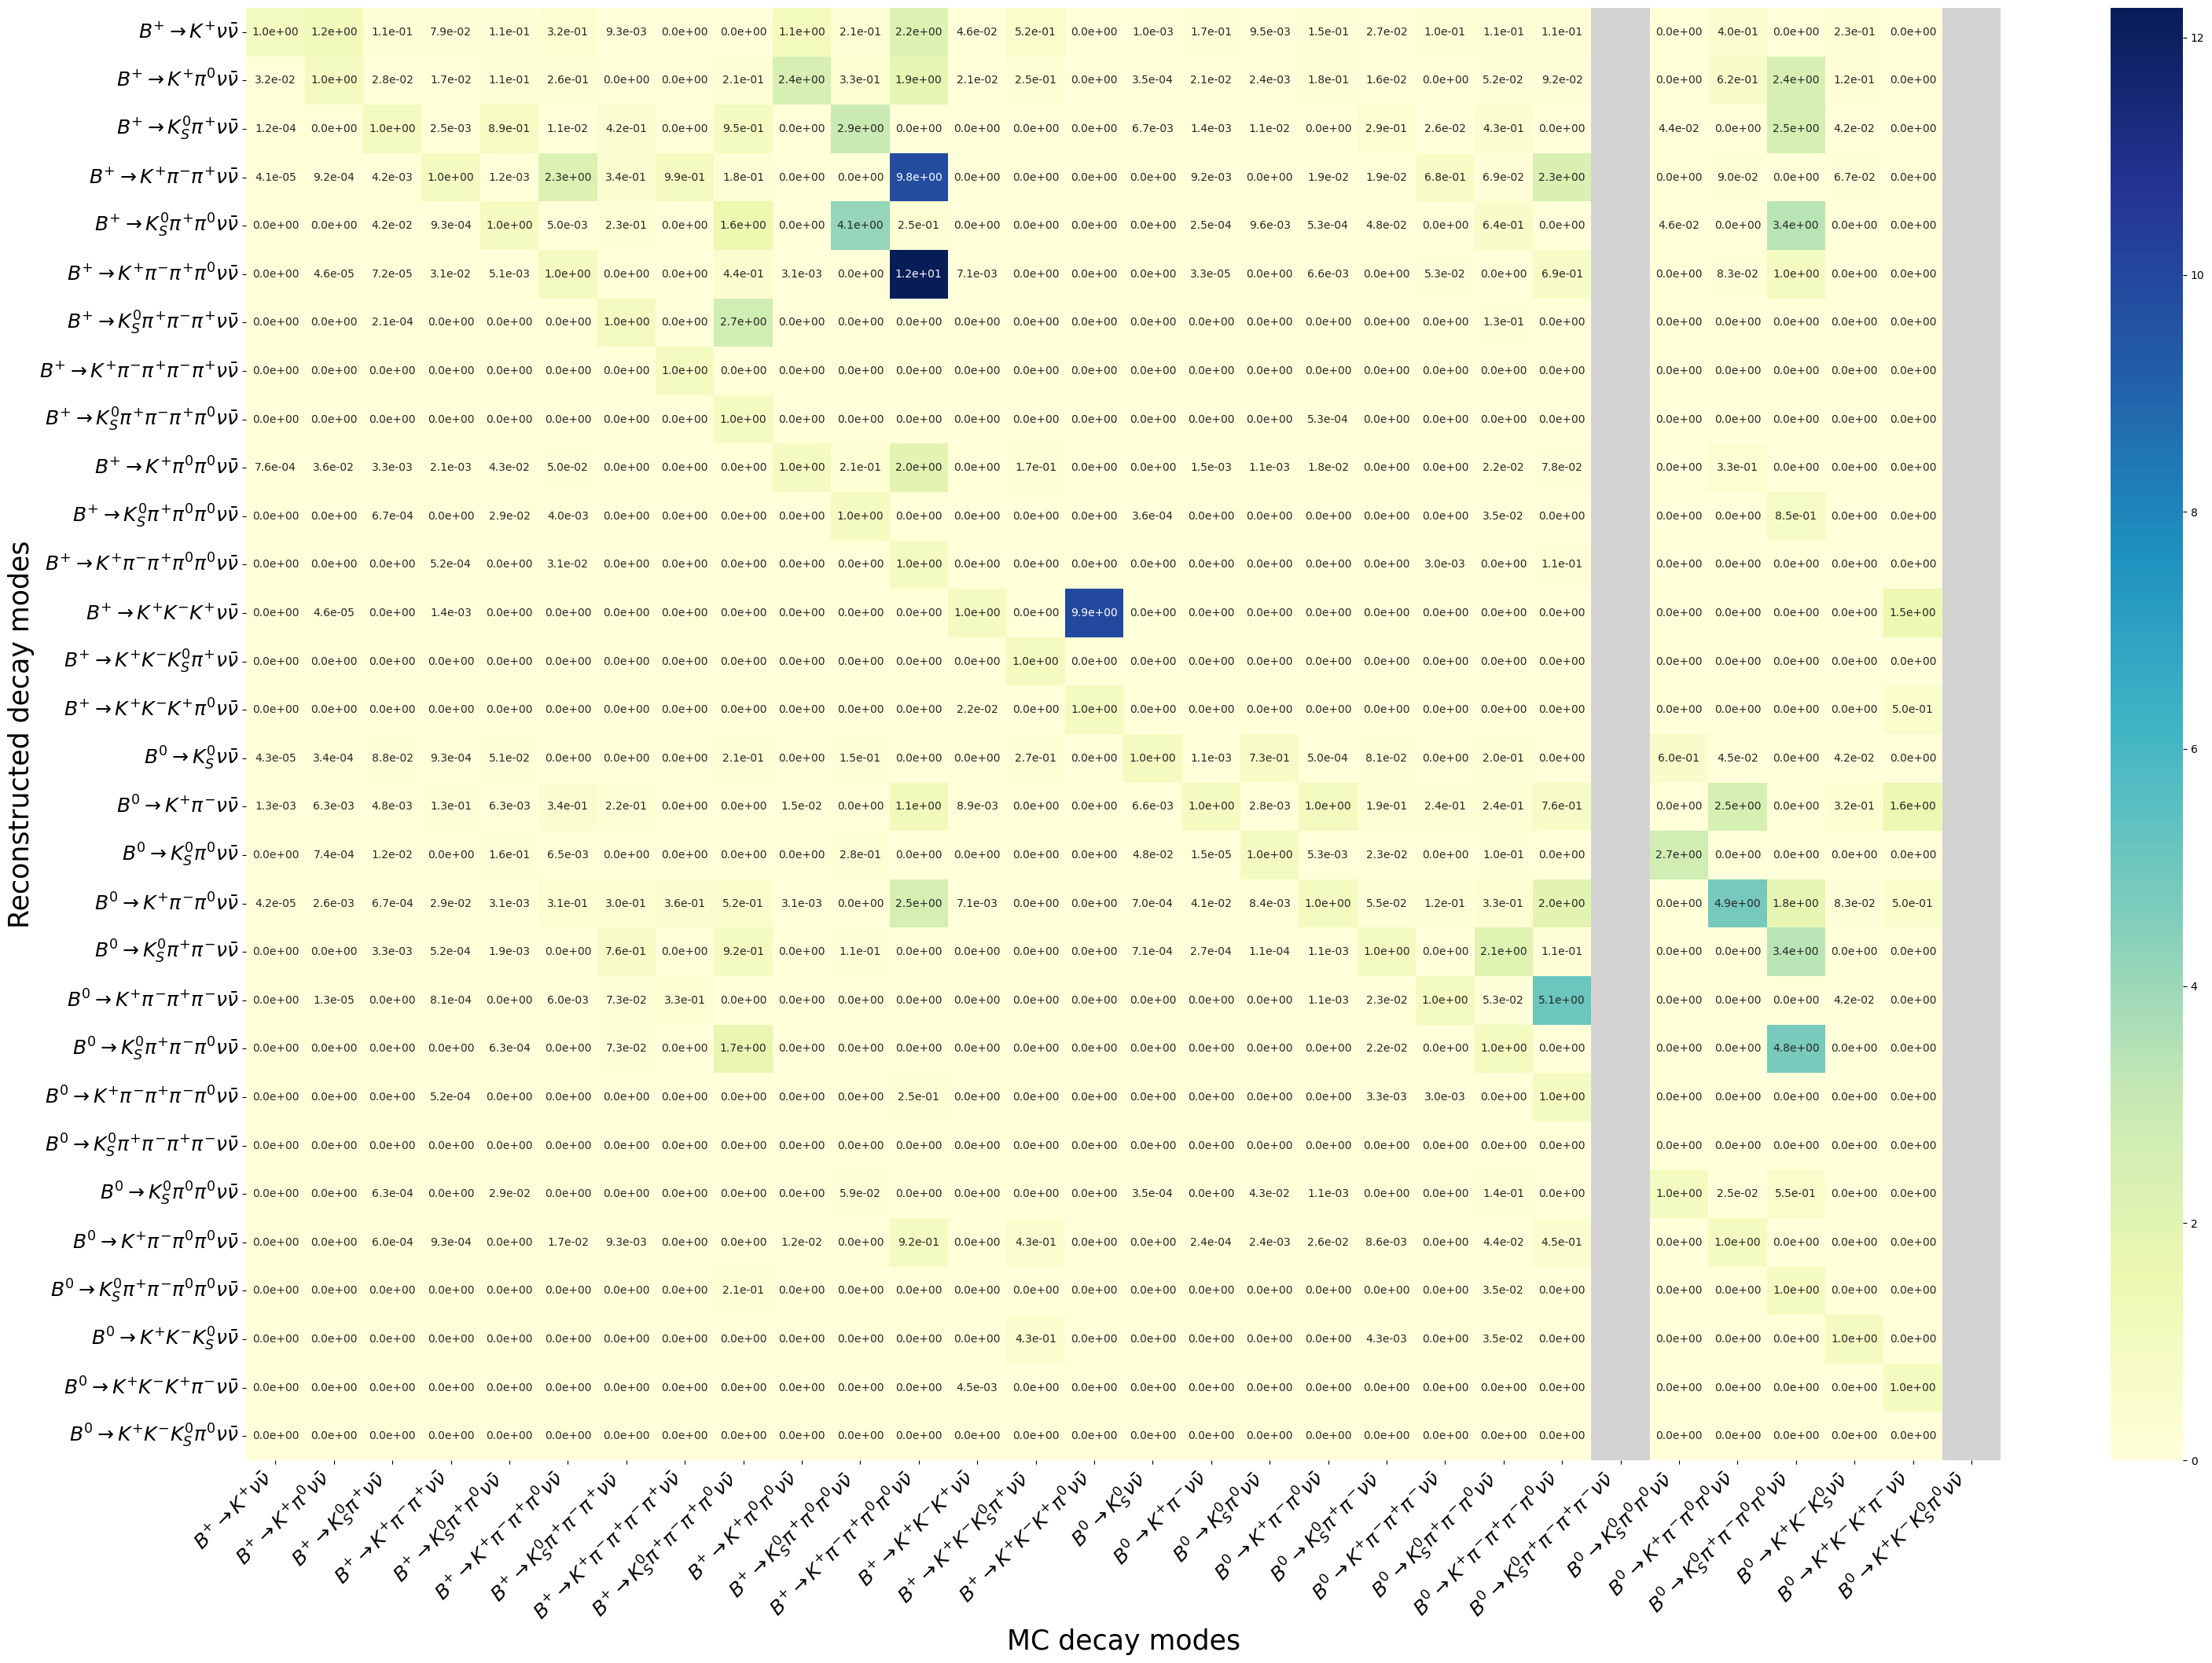
\includegraphics[width=0.9\textwidth]{./picture/cross_feed_matrix.png}
\caption{Cross-feed matrix. It is defined as $\epsilon_{\mathrm{mode}}/\epsilon_{\mathrm{true}}$, where $\epsilon_{\mathrm{mode}}$ is the efficiency for events to be reconstructed in a given mode, and $\epsilon_{\mathrm{true}}$ is the efficiency for events to be reconstructed in the correct decay mode.}
\label{fig:crossfeedmatrix}
\end{figure}

\chapter{Signal yield extraction strategy}
\section{Signal region definition}
\label{sec:signal_region}
In this analysis, we define the signal region in the two-dimensional $M_{X_{s}}^{\textrm{reco}}$--$\mathcal{O}_{\textrm{BDT}}$ plane.
Because $\mathcal{O}_{\textrm{BDT}}$ has different distributions depending on the value of $M_{X_{s}}^{\textrm{reco}}$, we use this two-dimensional region.
The signal region is defined by $0.0 < M_{X_{s}}^{\textrm{reco}} < 2.0~\textrm{GeV}/c^{2}$ and $0.86 < \mathcal{O}_{\textrm{BDT}} \leq 1.0$.

We divide the signal region into $3\times5$ bins.
The bin boundaries along the $M_{X_{s}}^{\textrm{reco}}$ axis are $[0.0, 0.6, 1.0, 2.0]~\textrm{GeV}/c^{2}$.
These three bins correspond to the regions dominated by $K$, $K^{*}$, and the remaining $X_{s}$ states.
Hereafter, we label them MR1, MR2, and MR3, respectively.
When the signal MC is produced, the mass threshold, $M_{X_{s}} > 1.1~\textrm{GeV}/c^{2}$, is required, as discussed in Section~\ref{subsec:signal_MC}.
The bin boundary between MR2 and MR3 is set to $1.0~\textrm{GeV}/c^{2}$, slightly below this threshold, to minimize sensitivity to the modeling of this threshold.
In each $M_{X_{s}}^{\textrm{reco}}$ region, the bin boundaries along $\mathcal{O}_{\textrm{BDT}}$ are defined as follows:
\begin{equation}
    \textrm{Bin boundary} = 
  \begin{cases}
    [0.86, 0.9195, 0.979, 0.986, 0.993, 1.0] & (\textrm{in MR1}), \\[10pt]
    [0.86, 0.8925, 0.925, 0.95, 0.975, 1.0] & (\textrm{in MR2}), \\[10pt]
    [0.86, 0.9, 0.94, 0.96, 0.98, 1.0] & (\textrm{in MR3}).
  \end{cases}
\end{equation}
These bin boundaries are determined to maximize the sensitivity while avoiding fit bias.
If small bin widths are used, the sensitivity improves.
However, if the number of events in the bin is small, the pull distribution of the signal strength does not follow a Gaussian distribution, as seen in Figure~\ref{fig:non-gaussian}.
Therefore, the number and size of bins are determined to fulfill these conditions.
\begin{figure}[h]
  \centering
  \subfloat{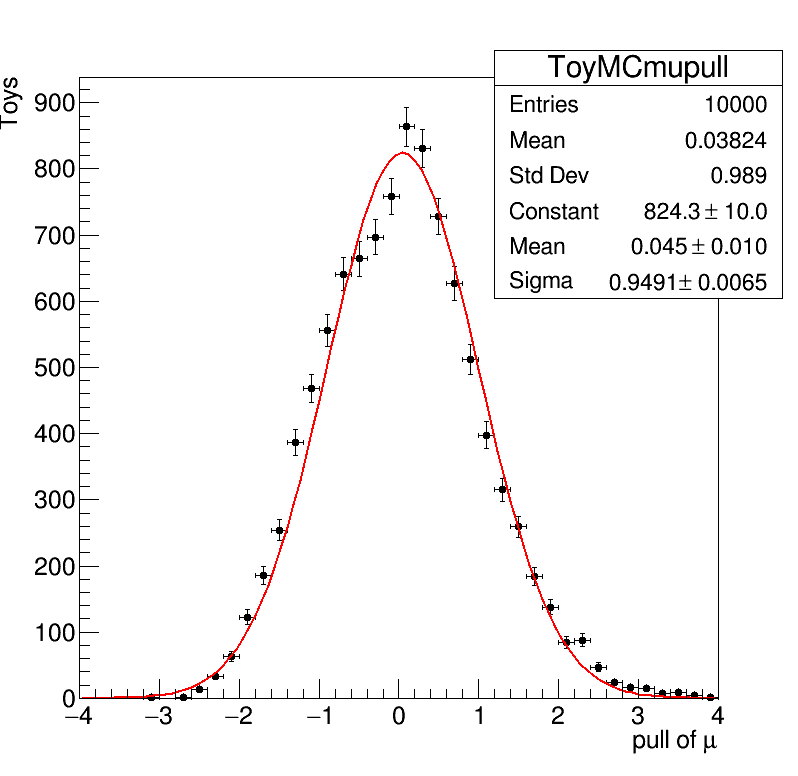
\includegraphics[width=0.65\textwidth]{./picture/bad_pull.png}}
  \caption{Pull distribution when the number of events in the bin is small.}
  \label{fig:non-gaussian}
\end{figure}

For simplicity, we define the variable ``bin index" and the mapping from $M_{X_{s}}^{\textrm{reco}}$-$\mathcal{O}_{\textrm{BDT}}$ plane to the bin index value.
The bin index ranges from 1 to 5 in MR1, from 6 to 10 in MR2, and from 11 to 15 in MR3, increasing along the positive $\mathcal{O}_{\textrm{BDT}}$ axis within each mass region.
Figure~\ref{fig:bin_index} shows the mapping between the $M_{X_{s}}^{\textrm{reco}}$-$\mathcal{O}_{\textrm{BDT}}$ bins and the bin indices.
The number inside each bin indicates the bin index value.
\begin{figure}
  \centering
  \subfloat{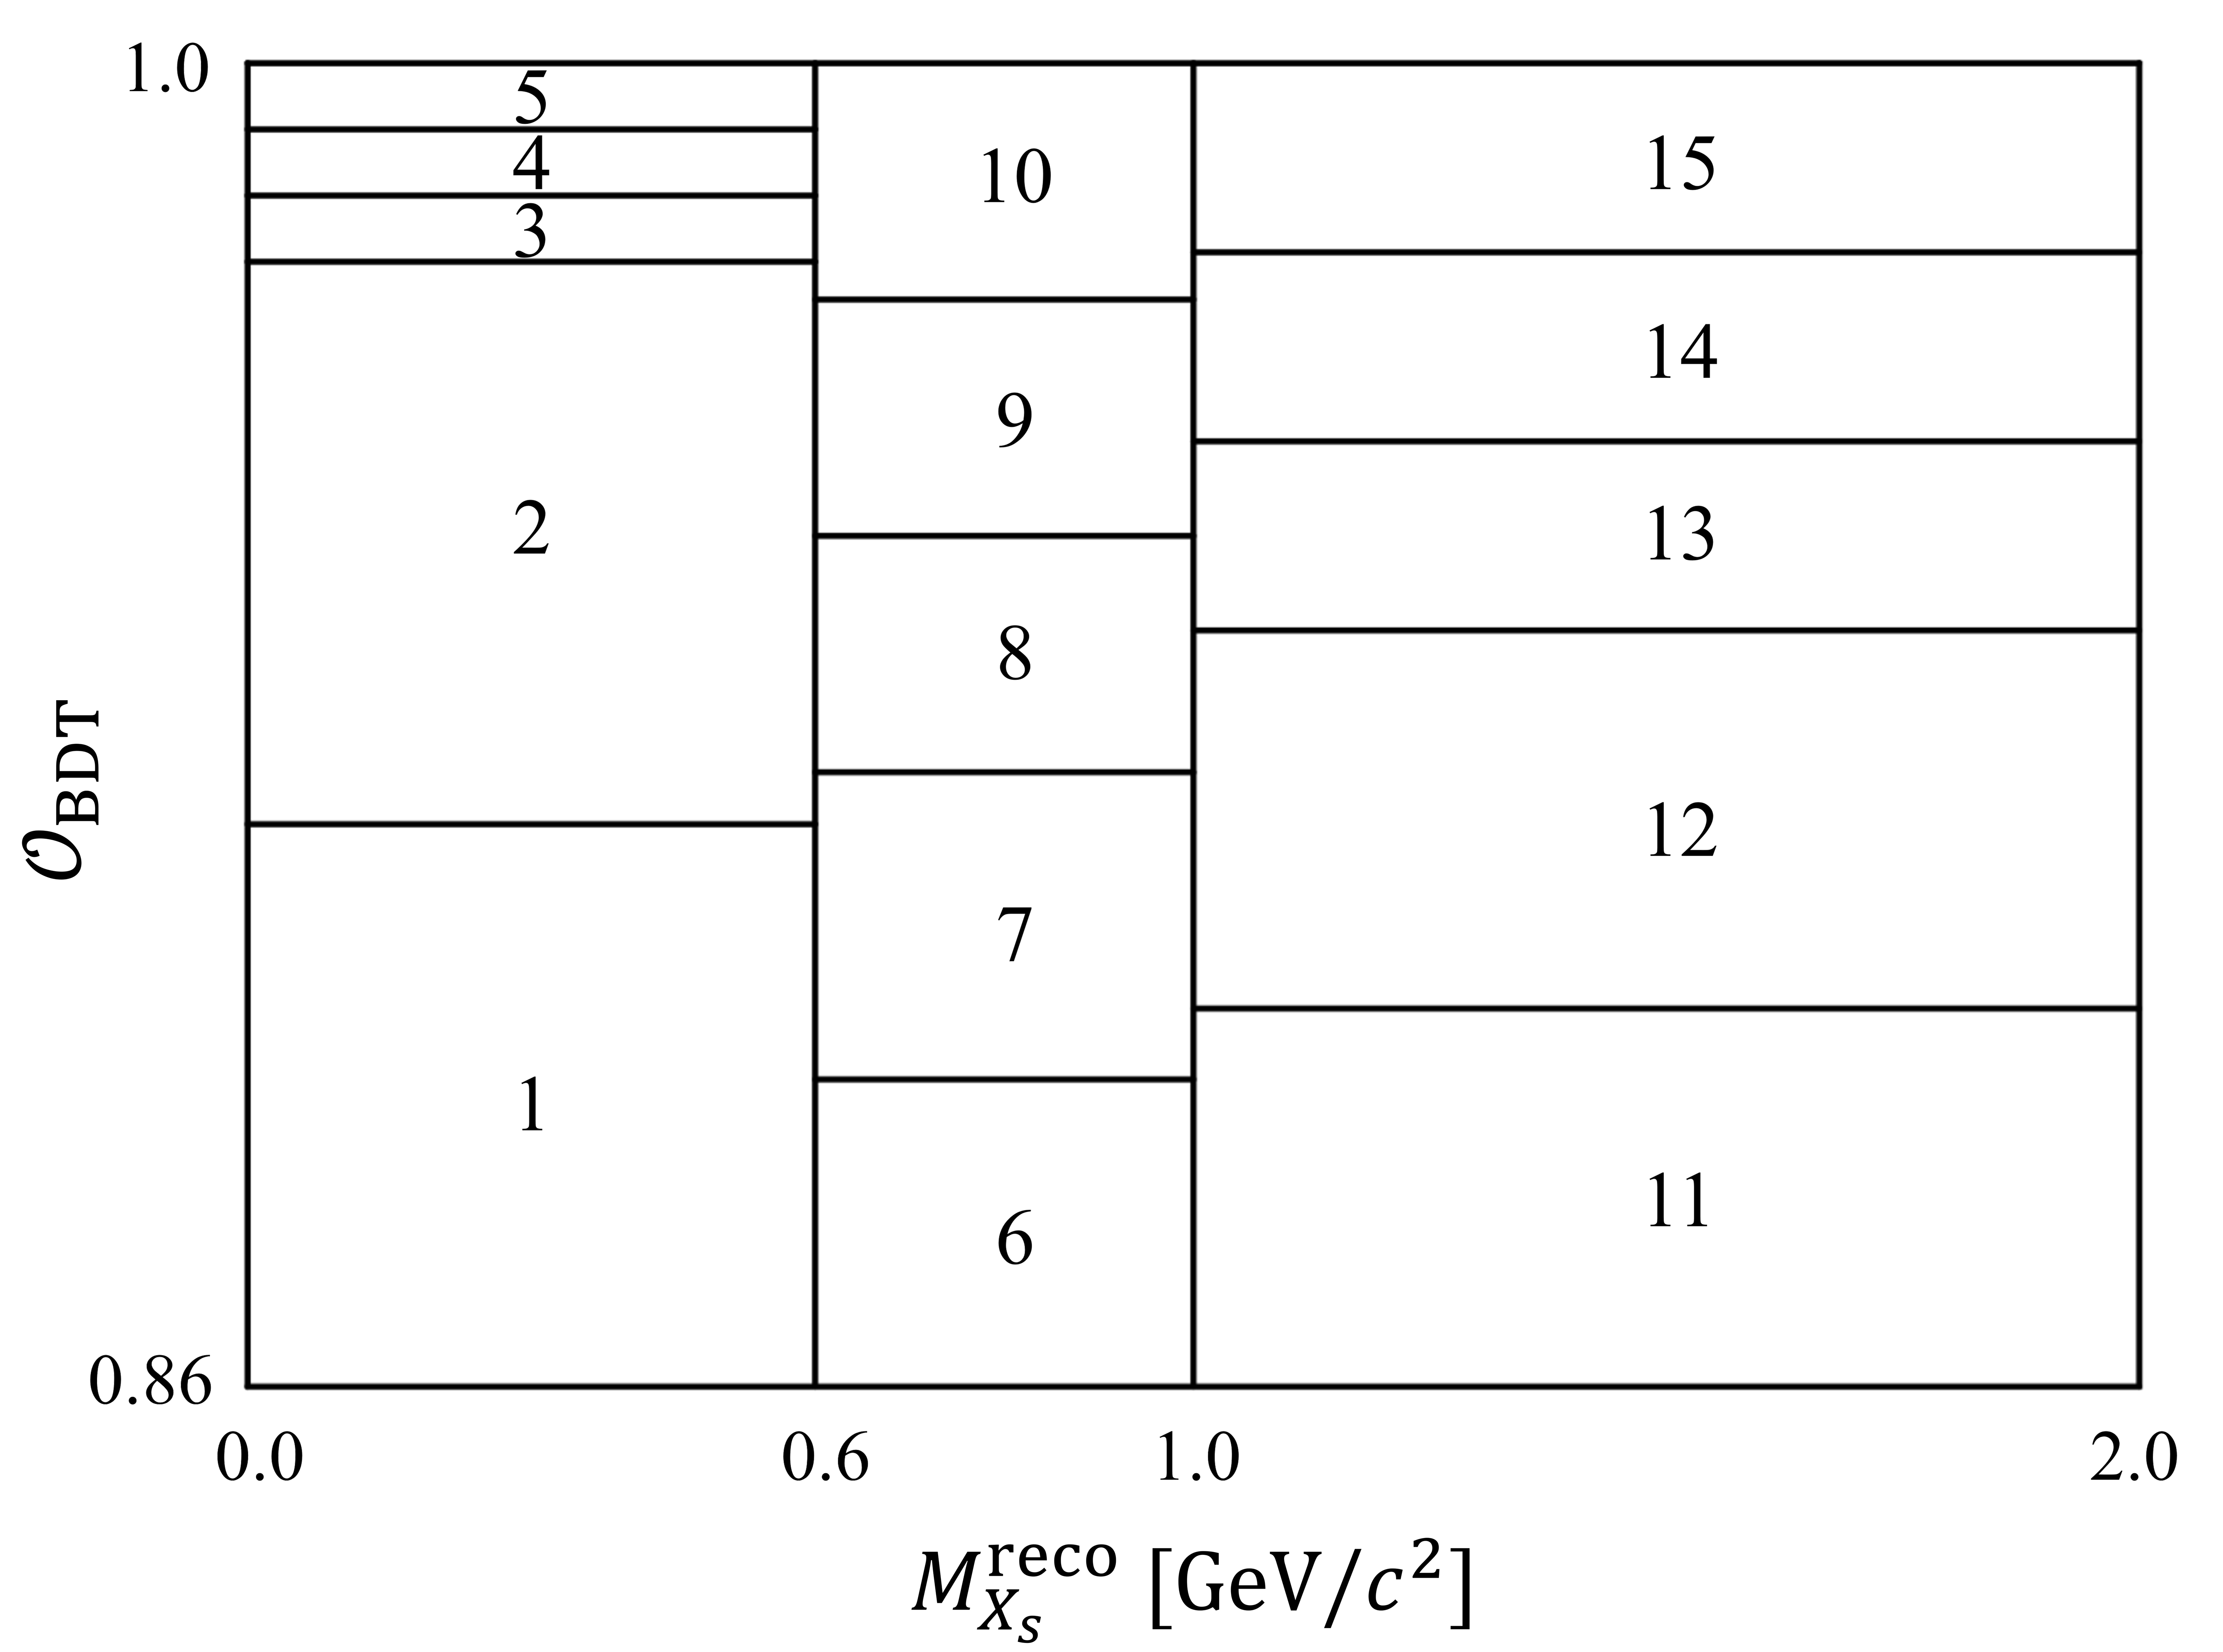
\includegraphics[width=0.65\textwidth]{./picture/bin_index.png}}
  \caption{Mapping between the two-dimensional $M_{X_{s}}^{\textrm{reco}}$--$\mathcal{O}_{\textrm{BDT}}$ bins and the bin indices.}
  \label{fig:bin_index}
\end{figure}
The bin index is used as the fitting variable.

Figure~\ref{fig:template_histogram} shows the bin index distributions for
the signal and background samples.
\begin{figure}
    \centering
    \subfloat[][Signal]{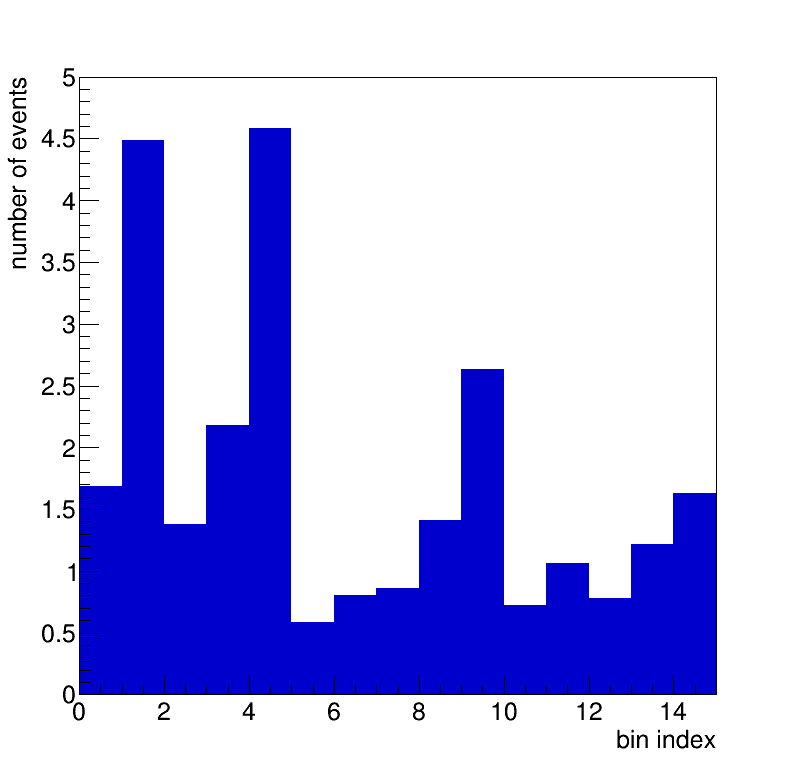
\includegraphics[width=0.5\textwidth]{./picture/histfactory/signal_hist.png}}
    \subfloat[][Background]{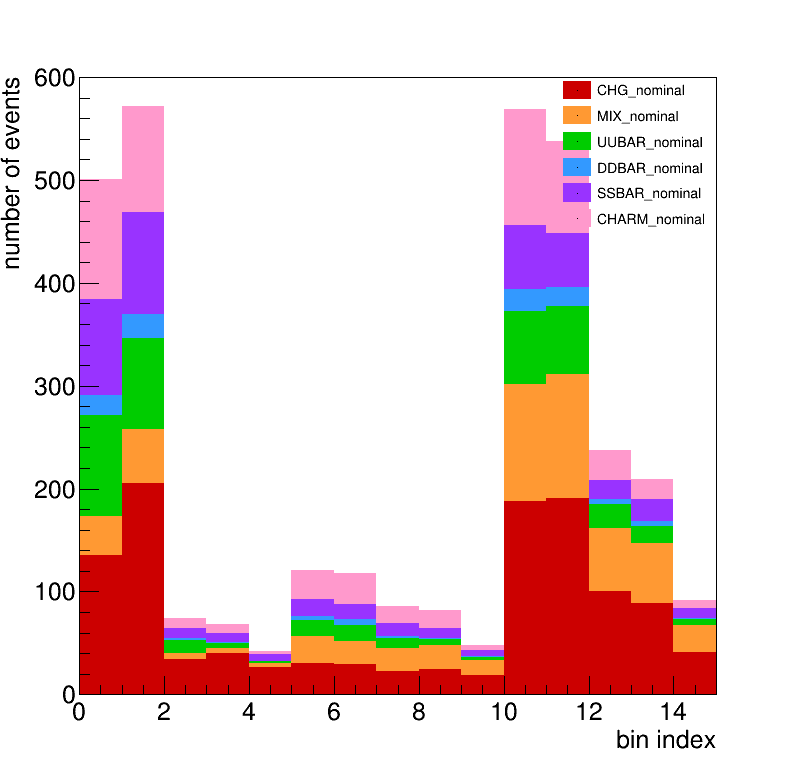
\includegraphics[width=0.5\textwidth]{./picture/histfactory/bkgs_hist.png}}
    \caption{Bin index distributions for the signal and background samples.}
    \label{fig:template_histogram}
\end{figure}

\section{Fitting strategy}
The tools \texttt{RooFit} and \texttt{RooStats} are used for fitting and limit setting.
A binned maximum-likelihood method is used.
To construct the probability density function, the tool \texttt{HistFactory}, provided within \texttt{RooStats}, is used~\cite{HistFactory}.
\texttt{HistFactory} provides an easy way to construct a probability density function.
It also gives a way to incorporate changes on shapes of histogram templates by systematic uncertainties.

\texttt{HistFactory} provides the following probability density function:
\begin{equation}
    \mathcal{P}(n_{cb}, a_{p}|\phi_{p},\alpha_{p},\gamma_{b}) = \prod_{\textrm{c}\in \textrm{channels}} \prod_{\textrm{b}\in \textrm{bins}} \textrm{Pois}(n_{cb}|\nu_{cb}) \cdot G(L_{0}|\lambda, \Delta_{L}) \cdot \prod_{p\in \mathbb{S}+\boldsymbol{\Gamma}} f_{p}(a_{p}|\alpha_{p}),
\end{equation}
where $n_{cb}$ is the number of observed events in channel $\textrm{c}$ and bin $\textrm{b}$, $f_{p}(a_{p}|\alpha_{p})$ is a constraint term for an auxiliary measurement $a_{p}$ with nuisance parameter $\alpha_{p}$.
In this analysis, all constraint terms, $f_p(a_p|\alpha_p)$, are Gaussian distributions.
The number of expected events is
\begin{equation}
    \nu_{cb}(\phi_{p},\alpha_{p},\gamma_{b})=\lambda_{cs}\gamma_{cb}\phi_{cs}(\alpha)\eta(\boldsymbol{\alpha})\sigma_{csb}(\boldsymbol{\alpha}),
\end{equation}
where
\begin{itemize}
  \item $\lambda_{cs}$: luminosity parameter for a given channel and sample.
  \item $\gamma_{cb}$: bin-by-bin scale factor used for statistical uncertainties, bin-by-bin shape systematics~(\texttt{ShapeSys}), and data-driven shape extrapolations~(\texttt{ShapeFactor}). For statistical uncertainties, $\gamma_{csb}$ is shared among all samples in the channel.
  \item $\phi_{cs}$: product of unconstrained normalization factors for a given sample within a given channel. These typically include the parameter of interest.
  \item $\eta_{cs}(\boldsymbol{\alpha})$: the parametrized normalization uncertainties~(\texttt{OverallSys}) for a given sample within a given channel.
  \item $\sigma_{csb}$: the parametrized histogram~(\texttt{HistoSys}) for a given sample within a given channel.
\end{itemize}

The branching ratios of $B\rightarrow K^{(*)}n\bar{n}$ decay is determined by the $B\rightarrow K^{(*)}p\bar{p}$ decays~\cite{ParticleDataGroup:2024cfk}.
The branching ratios of $B\rightarrow K^{(*)}n\bar{n}$ decay are estimated by isospin symmetry:
\begin{linenomath*}
  \begin{align}
    \textrm{BR}(B^{+} \rightarrow K^{+}n\bar{n}) = \textrm{BR}(B^{0} \rightarrow K^{0}p\bar{p}) \times \frac{\tau_{B^{+}}}{\tau_{B^{0}}},\\
    \textrm{BR}(B^{+} \rightarrow K^{*+}n\bar{n}) = \textrm{BR}(B^{0} \rightarrow K^{*0}p\bar{p}) \times \frac{\tau_{B^{+}}}{\tau_{B^{0}}},\\
    \textrm{BR}(B^{+} \rightarrow K^{0}n\bar{n}) = \textrm{BR}(B^{+} \rightarrow K^{+}p\bar{p}) \times \frac{\tau_{B^{0}}}{\tau_{B^{+}}},\\
    \textrm{BR}(B^{+} \rightarrow K^{*0}n\bar{n}) = \textrm{BR}(B^{+} \rightarrow K^{*+}p\bar{p}) \times \frac{\tau_{B^{0}}}{\tau_{B^{+}}},
\end{align}
\end{linenomath*}
where $\tau_{B^{+}}$ and $\tau_{B^{0}}$ are the life time of $B^{+}$ and $B^{0}$, respectively.
The weights are applied to satisfy the estimated branching ratios of $B\rightarrow K^{(*)}n\bar{n}$ decay.

In this analysis, three parameters of interest are defined: $\mu_{1}$, $\mu_{2}$, and $\mu_{3}$.
These parameters are signal strengths defined as follows:
\begin{equation}
  \label{eq:poi_3mu_fit}
  \begin{cases}
    \mu_{1} =& \frac{\textrm{Branching ratio in the} \; 0.0 < M_{X_{s}} < 0.6~\textrm{GeV}/c^{2} \textrm{ region, obtained from the fit}}{\textrm{Branching ratio in the} \; 0.0 < M_{X_{s}} < 0.6~\textrm{GeV}/c^{2} \textrm{ region in SM}}, \\[10pt]
    \mu_{2} =& \frac{\textrm{Branching ratio in the} \; 0.6 < M_{X_{s}} < 1.0~\textrm{GeV}/c^{2} \textrm{ region, obtained from the fit}}{\textrm{Branching ratio in the} \; 0.6 < M_{X_{s}} < 1.0~\textrm{GeV}/c^{2} \textrm{ region in SM}}, \\[10pt]
    \mu_{3} =& \frac{\textrm{Branching ratio in the} \; 1.0~\textrm{GeV}/c^{2} < M_{X_{s}} \textrm{ region, obtained from the fit}}{\textrm{Branching ratio in the} \; 1.0~\textrm{GeV}/c^{2} < M_{X_{s}} \textrm{ region in SM}}.
  \end{cases}
\end{equation}
As shown in Eq.~\ref{eq:poi_3mu_fit}, each signal-strength parameter is in one-to-one correspondence with the branching ratio in the corresponding mass region.

Alternatively, a single parameter of interest, $\mu$, can be defined as
\begin{equation}
  \label{eq:poi_1mu_fit}
  \mu = \frac{\textrm{Branching ratio over the entire} \; M_{X_{s}} \textrm{ region, obtained from the fit}}{\textrm{Branching ratio over the entire} \; M_{X_{s}} \textrm{ region in SM}}.
\end{equation}
However, this method assumes fixed relative signal strengths among the three $M_{X_{s}}$ regions and therefore relies on the signal modeling.
Consequently, the single-parameter approach is not used in this analysis.

\section{Limit setting strategy}
To set an upper limit on the branching ratio of $B\rightarrow X_{s}\nu \bar{\nu}$ decays, the $CL_{s}$ method is used~\cite{Read:2002hq}.
The $CL_{s}$ method provides a conservative procedure for setting upper limits.
In this section, the $CL_{s+b}$ method is first described, followed by the motivation for using the $CL_{s}$ method.

Let $\mu$ be the parameter of interest, such as a branching ratio or a signal strength.
The goal is to test whether a specific value, $\mu_{\textrm{test}}$, is compatible with the observed data.
If $\mu_{\textrm{test}}$ is too large to describe the observed data, this value can be excluded.

For this purpose, a test statistic $q_{\mu}(x)$ is defined, which maps a dataset $x$ to a single real number.
The convention adopted here is that a larger value of $q_{\mu}(x)$ corresponds to greater incompatibility between the tested value of $\mu$ and the dataset $x$.

Consequently, a large value of $q_{\mu_{\textrm{test}}}(x_{\textrm{obs}})$ indicates that $\mu_{\textrm{test}}$ is incompatible with the observed data $x_{\textrm{obs}}$.
To quantify this incompatibility, toy MC samples are generated under the hypothesis $\mu=\mu_{\textrm{test}}$: $x_{\textrm{toy},1}$, $x_{\textrm{toy},2}$, $\dots$.
From these toys, we can obtain the distribution of $q_{\mu_{\textrm{test}}}(x)$.
The corresponding p-value, denoted by $CL_{s+b}$, is then defined as
\begin{equation}
    CL_{s+b}=\mathcal{P}(q>q_\mu(x_{\textrm{obs}})|\mu=\mu_{\textrm{test}}).
\end{equation}
For example, if $CL_{s+b}=0.03$, then, assuming $\mu_{\textrm{test}}$ is the true value, the probability of obtaining data that are more incompatible than the observed data is 0.03.

To obtain an upper limit, $CL_{s+b}$ is scanned as a function of $\mu_{\textrm{test}}$.
The 90\% confidence-level upper limit, $\mu_{\textrm{UL}}$, is obtained from the condition
\begin{equation}
    CL_{s+b}(\mu_{\textrm{UL}}) = 0.1.
\end{equation}

However, even in the absence of sensitivity, the $CL_{s+b}$ method can exclude the signal because of a downward statistical fluctuation of the background.
To avoid such false exclusions, the p-value under the background-only hypothesis, $CL_{b}$, is also calculated:
\begin{equation}
    CL_{b}=\mathcal{P}(q>q_\mu(x_{\textrm{obs}})|\mu=0).
\end{equation}
The $CL_{s}$ value is then defined as
\begin{equation}
    CL_{s}=\frac{CL_{s+b}}{CL_{b}}.
\end{equation}

The use of $CL_{s}$ helps avoid false exclusions.
For example, if the experiment has no sensitivity to the signal, the signal-plus-background and background-only hypotheses give identical distributions of the test statistic.
In this case, the $CL_{s+b}$ method would still exclude the signal with 10\% probability at the 90\% confidence level.
However, since $CL_{s+b}=CL_{b}$, one obtains $CL_{s}=1$, and the signal is not excluded.

In this analysis, the one-sided negative log profile likelihood ratio is used as the test statistic:
\begin{equation}
    q_{\mu} =
    \begin{cases}
        -\ln\lambda(\mu), & \hat{\mu} < \mu,\\
        0, & \hat{\mu} \geq \mu,
    \end{cases}
\end{equation}
where $\hat{\mu}$ is the signal strength obtained from the best fit to the data.

\chapter{Validation}
\label{sec:validation}
\section{Off-resonance}
\label{sec:off_resonance}
The off-resonance sample is used for two purposes.
First, it is used to check the data--MC agreement of the FastBDT input variables.
Second, it is used to obtain correction factors and their uncertainties.
For this study, we use off-resonance data and off-resonance $e^{+}e^{-}\rightarrow q\bar{q}$ MC samples.

We use a cut flow similar to that shown in Table~\ref{tab:cutflow}.
However, $M_{\textrm{bc}}$ distribution is shifted because of the lower center-of-mass energy.
Therefore, we correct the $M_{\textrm{bc}}$ values for both data and MC:
\begin{equation}
  \label{eq:Mbc_corr}
  M_{\textrm{bc, corrected}} = \sqrt{(\sqrt{s^{\textrm{off}}}/2)^{2}-|\vec{p}_{B}^{*}c|^{2}}+(\sqrt{s^{\textrm{on}}}-\sqrt{s^{\textrm{off}}})/2,
\end{equation}
where $\sqrt{s^{\textrm{on}}}$ and $\sqrt{s^{\textrm{off}}}$ are the SuperKEKB c.m. energies for the on-resonance and off-resonance samples, respectively.
In this analysis, $\sqrt{s^{\textrm{on}}}$ is set to the center-of-mass energy used for the run-independent MC sample.
No correction is applied to $\Delta E$, because its distribution is not shifted.

Figures~\ref{fig:off_used_vars1}--\ref{fig:off_used_vars2} show the distributions of the FastBDT input variables.
MC distributions are scaled to the data in the figures.
The overall event yields in data and MC show a discrepancy.
After the FastBDT requirement, the data-to-MC ratios are
\begin{equation}
\label{eq:off_resonance_ratio}
    \frac{\textrm{Data}}{\textrm{MC}} = 
  \begin{cases}
    1.21 \pm 0.13 & (0.0 < M_{X_{s}}^{\textrm{reco}} < 0.6~\textrm{GeV}), \\[10pt]
    0.90 \pm 0.20 & (0.6 \leq M_{X_{s}}^{\textrm{reco}} < 1.0~\textrm{GeV}), \\[10pt]
    0.78 \pm 0.10 & (1.0 \leq M_{X_{s}}^{\textrm{reco}} < 2.0~\textrm{GeV}).
  \end{cases}
\end{equation}
These ratios are obtained after applying the calibration and correction factors listed in Section~\ref{sec:correction}, \underline{except} for the $q\bar{q}$ correction factor.

Table~\ref{tab:cutflow_off} shows the cut flow for the off-resonance sample.
Figure~\ref{fig:FBDT_off} shows the FastBDT output distribution.
\begin{table}
\caption{Cut flow for off-resonance sample. The entries show the numbers of events surviving each selection requirement. MC samples are scaled to $42.74~\textrm{fb}^{-1}$. Calibration and correction factors listed in Section~\ref{sec:correction} are \underline{not} applied in this table.}
  \renewcommand{\arraystretch}{1.2}
  \centering
\begin{tabular}{ p{7cm} ||  p{3cm} | p{3cm} | p{3cm}  }
 \hline
  \hline
Selection &  \multicolumn{1}{c}{data} & \multicolumn{1}{c|}{MC} & \multicolumn{1}{c}{data/MC}\\
 \hline
Generated & \multicolumn{1}{c}{$42.74~\textrm{fb}^{-1}$} & \multicolumn{1}{c|}{$42.74~\textrm{fb}^{-1}$} & \multicolumn{1}{c}{1.0} \\
Skim & \multicolumn{1}{c}{$2.35\cdot10^{7}$} & \multicolumn{1}{c|}{$2.20\cdot10^{7}$}& \multicolumn{1}{c}{1.0693} \\
Reconstruction and preselections & \multicolumn{1}{c}{113586} & \multicolumn{1}{c|}{123254}& \multicolumn{1}{c}{0.9216} \\
$M_{\textrm{bc}}$ correction & \multicolumn{1}{c}{113586} & \multicolumn{1}{c|}{123254}& \multicolumn{1}{c}{0.9216} \\
$M_{\textrm{bc, corrected}}>5.27~\textrm{GeV}/c^{2}$ for $B_{\textrm{tag}}$ & \multicolumn{1}{c}{31402} & \multicolumn{1}{c|}{35143}& \multicolumn{1}{c}{0.8935} \\
$\left|\Delta E \right|<0.2~\textrm{GeV}$ for $B_{\textrm{tag}}$ & \multicolumn{1}{c}{29851} & \multicolumn{1}{c|}{33328}& \multicolumn{1}{c}{0.8957} \\
$E_{\textrm{ecl}}<1.3~\textrm{GeV}$ & \multicolumn{1}{c}{16423} & \multicolumn{1}{c|}{18155}& \multicolumn{1}{c}{0.9046} \\
$17^\circ < \theta_{\textrm{missing}} < 150^\circ$ & \multicolumn{1}{c}{14092} & \multicolumn{1}{c|}{15485}& \multicolumn{1}{c}{0.9100} \\
$0.5<p_{X_{s}}^{*}<2.96~\textrm{GeV}/c$ & \multicolumn{1}{c}{13034} & \multicolumn{1}{c|}{14229}& \multicolumn{1}{c}{0.9160} \\
Reject $1.84 < M_{X_{s}}^{\textrm{reco}} < 1.89~\textrm{GeV}/c^{2}$ & \multicolumn{1}{c}{12418} & \multicolumn{1}{c|}{13645}& \multicolumn{1}{c}{0.9187} \\
BCS & \multicolumn{1}{c}{12418} & \multicolumn{1}{c|}{13645}& \multicolumn{1}{c}{0.9187} \\
$\mathcal{O}_{\textrm{BDT}} > 0.86$ & \multicolumn{1}{c}{208} & \multicolumn{1}{c|}{225.4}& \multicolumn{1}{c}{0.9228} \\
  \hline
   \hline
\end{tabular}
    \label{tab:cutflow_off}
\end{table}
\begin{figure}
    \centering
    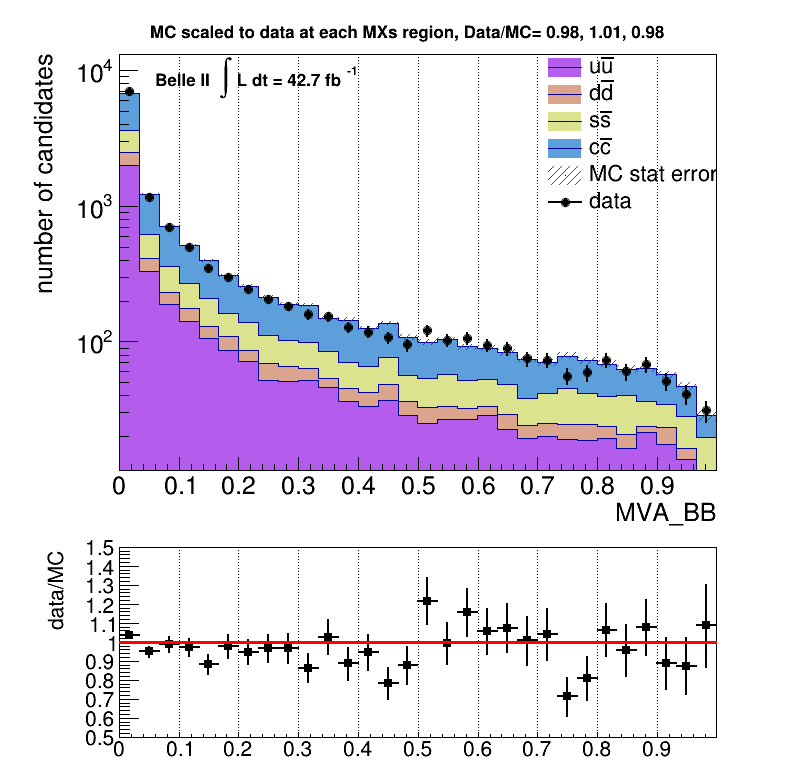
\includegraphics[width=0.48\textwidth]{./picture/off/MVA_BB_offres.png}
    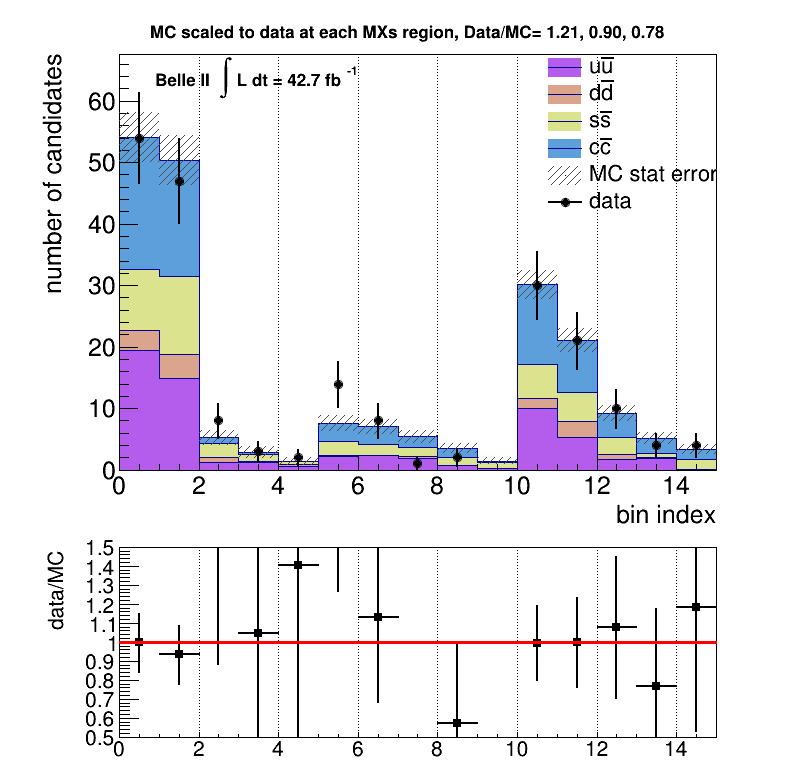
\includegraphics[width=0.48\textwidth]{./picture/off/bin_index_offres.png}
    \caption{The left plot shows the FastBDT output distribution for the off-resonance sample. The right plot shows the distribution of the bin index defined in Section~\ref{sec:signal_region}. Calibration and correction factors listed in Section~\ref{sec:correction} are applied, \underline{except} for the $q\bar{q}$ correction factor.}
    \label{fig:FBDT_off}
\end{figure}

\section{On-resonance $M_{\textrm{bc}}$ sideband}
During the selection procedure in Section~\ref{sec:selection}, we apply the following requirement on $M_{\textrm{bc}}$:
\begin{equation}
  M_{\textrm{bc}} > 5.27~\textrm{GeV}/c^{2}.
\end{equation}
We define an $M_{\textrm{bc}}$ sideband as
\begin{equation}
  5.235 < M_{\textrm{bc}} < 5.26~\textrm{GeV}/c^{2}.
\end{equation}
The region $5.26 < M_{\textrm{bc}} < 5.27~\textrm{GeV}/c^{2}$ is not included in the sideband to ensure sufficient separation from the signal region.
Table~\ref{tab:cutflow_sideband_on} shows the cut flow for the sideband study. 
\begin{table}
\caption{Cut flow for the on-resonance $M_{\textrm{bc}}^{\textrm{tag}}$ sideband sample. The entries show the numbers of events surviving each selection requirement. The MC samples are scaled to an integrated luminosity of $365.4~\textrm{fb}^{-1}$. Calibration and correction factors listed in Section~\ref{sec:correction} are not applied in this table.}
  \renewcommand{\arraystretch}{1.2}
  \centering
  \resizebox{\textwidth}{!}{%
\begin{tabular}{ l ||  c | c | c  }
 \hline
  \hline
Selection &  \multicolumn{1}{c}{data} & \multicolumn{1}{c|}{MC} & \multicolumn{1}{c}{data/MC}\\
 \hline
Generated & \multicolumn{1}{c}{$365.4~\textrm{fb}^{-1}$} & \multicolumn{1}{c|}{$365.4~\textrm{fb}^{-1}$} & \multicolumn{1}{c}{1.0} \\
Skim & \multicolumn{1}{c}{$3.01 \cdot 10^{8}$} & \multicolumn{1}{c|}{$2.87 \cdot 10^{8}$}& \multicolumn{1}{c}{1.0469} \\
Reconstruction, preselections, and $M_{\textrm{bc}}<5.26~\textrm{GeV}/c^{2}$ & \multicolumn{1}{c}{1115436} & \multicolumn{1}{c|}{1233668}& \multicolumn{1}{c}{0.9042} \\
$M_{\textrm{bc}}>5.235~\textrm{GeV}/c^{2}$ & \multicolumn{1}{c}{531606} & \multicolumn{1}{c|}{586715}& \multicolumn{1}{c}{0.9061} \\
$\left|\Delta E \right|<0.2~\textrm{GeV}$ & \multicolumn{1}{c}{504049} & \multicolumn{1}{c|}{556703}& \multicolumn{1}{c}{0.9054} \\
$E_{\textrm{ecl}}<1.3~\textrm{GeV}$ & \multicolumn{1}{c}{277954} & \multicolumn{1}{c|}{305240}& \multicolumn{1}{c}{0.9106} \\
$17^\circ < \theta_{\textrm{missing}} < 150^\circ$ & \multicolumn{1}{c}{235494} & \multicolumn{1}{c|}{257390}& \multicolumn{1}{c}{0.9149} \\
$0.5<p_{X_{s}}^{*}<2.96~\textrm{GeV}/c$ & \multicolumn{1}{c}{216586} & \multicolumn{1}{c|}{236273}& \multicolumn{1}{c}{0.9167} \\
Reject $1.84 < M_{X_{s}}^{\textrm{reco}} < 1.89~\textrm{GeV}/c^{2}$ & \multicolumn{1}{c}{207587} & \multicolumn{1}{c|}{225963}& \multicolumn{1}{c}{0.9187} \\
BCS & \multicolumn{1}{c}{207587} & \multicolumn{1}{c|}{225963}& \multicolumn{1}{c}{0.9187} \\
$\mathcal{O}_{\textrm{BDT}} > 0.86$ & \multicolumn{1}{c}{4767} & \multicolumn{1}{c|}{5067}& \multicolumn{1}{c}{0.9407} \\
  \hline
   \hline
\end{tabular}
}
    \label{tab:cutflow_sideband_on}
\end{table}

Figures~\ref{fig:sideband_used_vars1}-\ref{fig:sideband_used_vars2} show the distributions of the FastBDT input variables.
The event yields in data and MC show a discrepancy.
After the FastBDT requirement, the data-to-MC ratio is
\begin{equation}
    \frac{\textrm{Data}}{\textrm{MC}} = 
  \begin{cases}
    1.12 \pm 0.03 & (0.0 < M_{X_{s}}^{\textrm{reco}} < 0.6~\textrm{GeV}), \\[10pt]
    1.04 \pm 0.05 & (0.6 \leq M_{X_{s}}^{\textrm{reco}} < 1.0~\textrm{GeV}), \\[10pt]
    1.10 \pm 0.03 & (1.0 \leq M_{X_{s}}^{\textrm{reco}} < 2.0~\textrm{GeV}).
  \end{cases}
\end{equation}
These ratios are obtained after applying the calibration and correction factors listed in Section~\ref{sec:correction}, including the $q\bar{q}$ correction factor.
The $q\bar{q}$ correction factor is calculated using the off-resonance sample, following the cut flow in Table~\ref{tab:cutflow_sideband_on}, with the $M_{\textrm{bc}}$ correction defined in Eq.~\ref{eq:Mbc_corr}.
The MC distributions are normalized to the data in Figure~\ref{fig:sideband_used_vars1}-\ref{fig:sideband_used_vars2}.
$q\bar{q}$ correction factor is \underline{not} applied in Figure~\ref{fig:sideband_used_vars1}-\ref{fig:sideband_used_vars2}.

Figure~\ref{fig:FBDT_sideband_on} shows the distribution of the bin index defined in Section~\ref{sec:signal_region}.
\begin{figure}
    \centering
    \subfloat{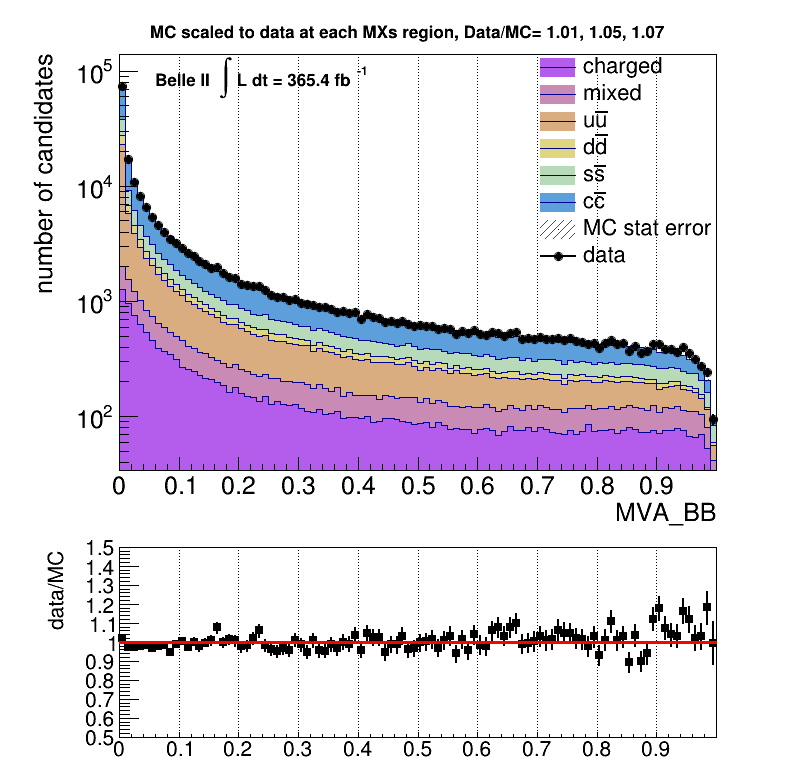
\includegraphics[width=0.5\textwidth]{./picture/sideband/MVA_BB_sideband.png}}
        \subfloat{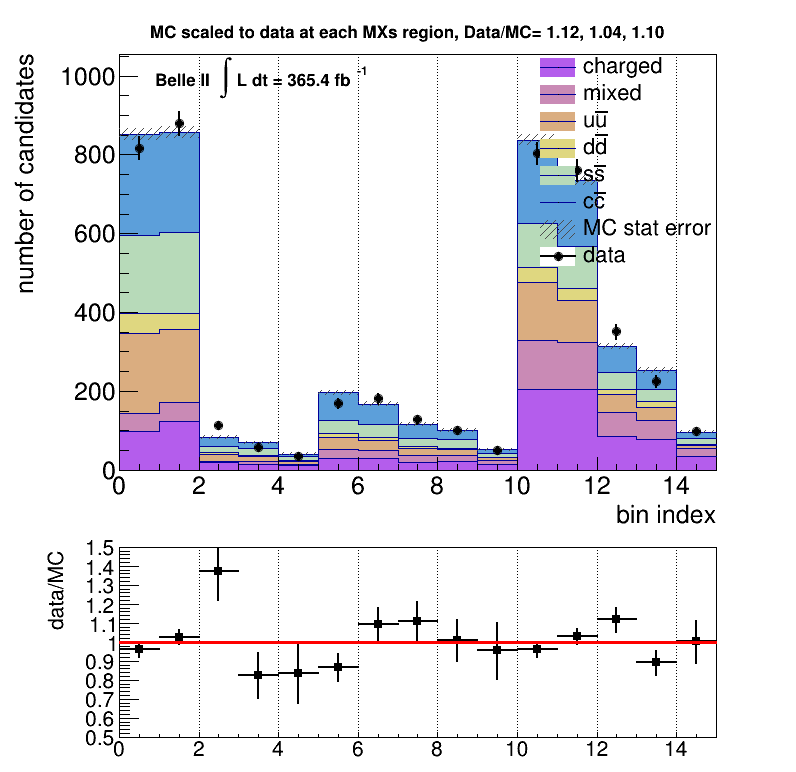
\includegraphics[width=0.5\textwidth]{./picture/sideband/bin_index_sideband.png}}
    \caption{The left plot shows the FastBDT output distribution for the on-resonance sideband sample. The right plot shows the distribution of the bin index defined in Section~\ref{sec:signal_region}. In both plots, calibration and correction factors listed in Section~\ref{sec:correction} are applied, including $q\bar{q}$ correction factor.}
    \label{fig:FBDT_sideband_on}
\end{figure}
There seems to be some deviation between data and MC in the region $0.0 < M_{X_{s}}^{\textrm{reco}} < 0.6~\textrm{GeV}$.
If the assigned systematic uncertainties account for this discrepancy, no additional systematic uncertainty or correction is required.
To evaluate this quantitatively, a fit is performed.
Figure~\ref{fig:FBDT_sideband_on_postfit} shows the FastBDT output distribution after the fit.
After the fit, the $\chi^{2}$ for the first region is
\begin{equation}
    \chi^{2}_{5} = 8.34 \; (0.0 < M_{X_{s}}^{\textrm{reco}} < 0.6~\textrm{GeV}).
\end{equation}
Then, the p-value is
\begin{equation}
    \textrm{p-value} = \mathcal{P}(\chi^{2}_{5} > 8.34) = 0.14 \; (0.0 < M_{X_{s}}^{\textrm{reco}} < 0.6~\textrm{GeV}),
\end{equation}
which is an acceptable value.
Consequently, the assigned systematic uncertainties can account for the data-MC discrepancy.
\begin{figure}
  \centering
  \subfloat{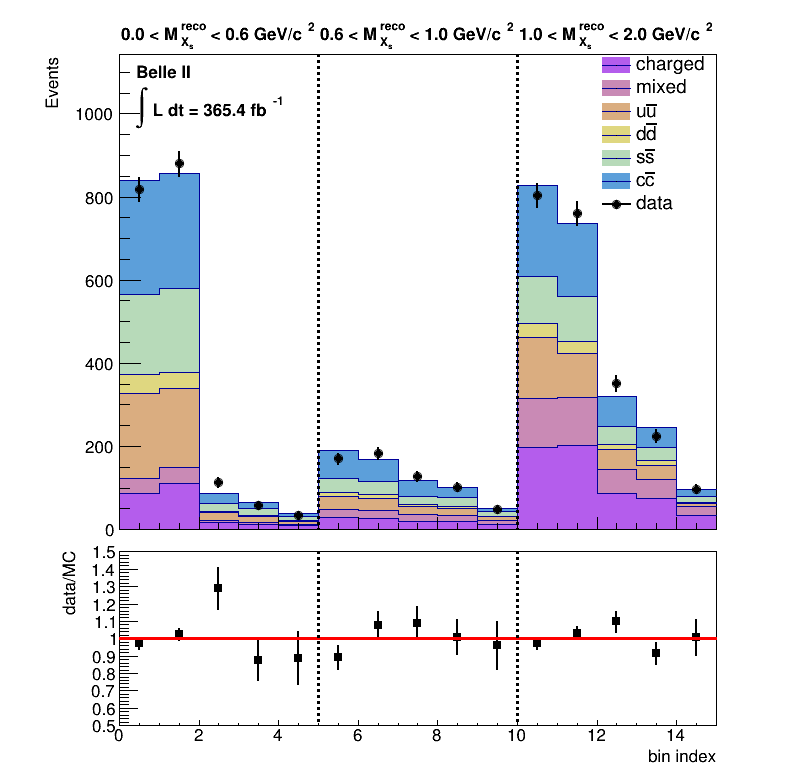
\includegraphics[width=0.5\textwidth]{./picture/sideband/FBDT_index_sideband_postfit.png}}
  \caption{The bin index distribution after the fit in the $M_{\textrm{bc}}$ sideband. The $p$-value is 0.14 in the region $0.0 < M_{X_{s}}^{\textrm{reco}} < 0.6~\textrm{GeV}/c^{2}$.}
  \label{fig:FBDT_sideband_on_postfit}
\end{figure}

\section{FastBDT sideband}
For validation, the FastBDT sideband is also examined.
This sideband is defined as
\begin{equation}
    0.8 < \mathcal{O}_{\textrm{BDT}} < 0.86.
\end{equation}
This region is dominated by background.

The cut flow shown in Table~\ref{tab:cutflow} is used.
However, the requirement $0.8 < \mathcal{O}_{\textrm{BDT}} < 0.86$ is applied instead of $\mathcal{O}_{\textrm{BDT}} > 0.86$.
Additionally, the off-resonance sample sample is analyzed to obtain the $q\bar{q}$ correction factor for the FastBDT sideband.

Figure~\ref{fig:FBDT_sideband_distribution} shows the FastBDT output distribution for each $M_{X_{s}}^{\textrm{reco}}$ region.
\begin{figure}
  \centering
  \subfloat[][$0.0 < M_{X_{s}}^{\textrm{reco}} < 0.6~\textrm{GeV}/c^{2}$]{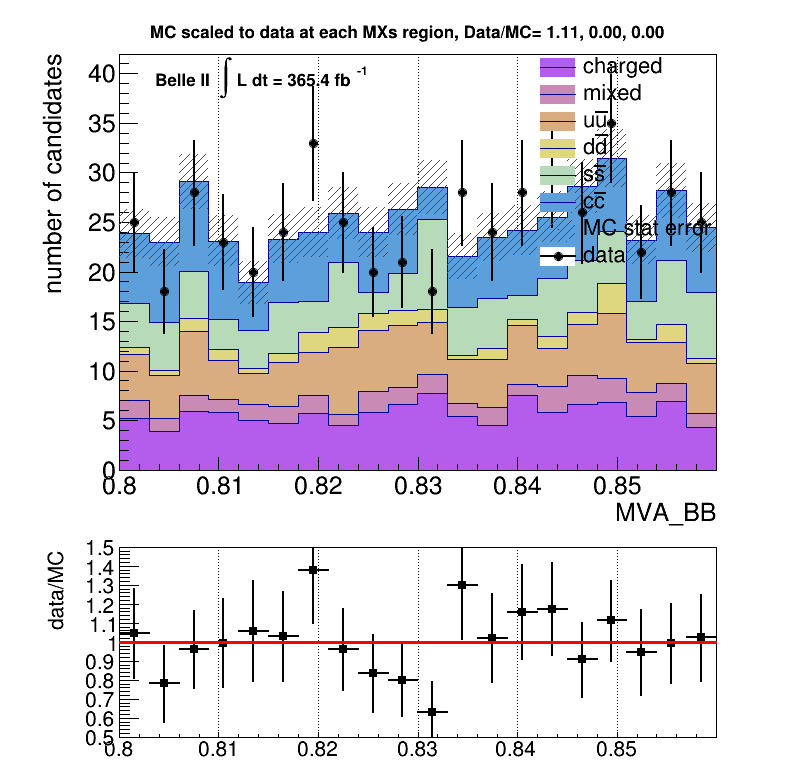
\includegraphics[width=0.3\textwidth]{./picture/FBDT_sideband/MVA_BB_sideband_MXs1.png}}
  \subfloat[][$0.6 \leq M_{X_{s}}^{\textrm{reco}} < 1.0~\textrm{GeV}/c^{2}$]{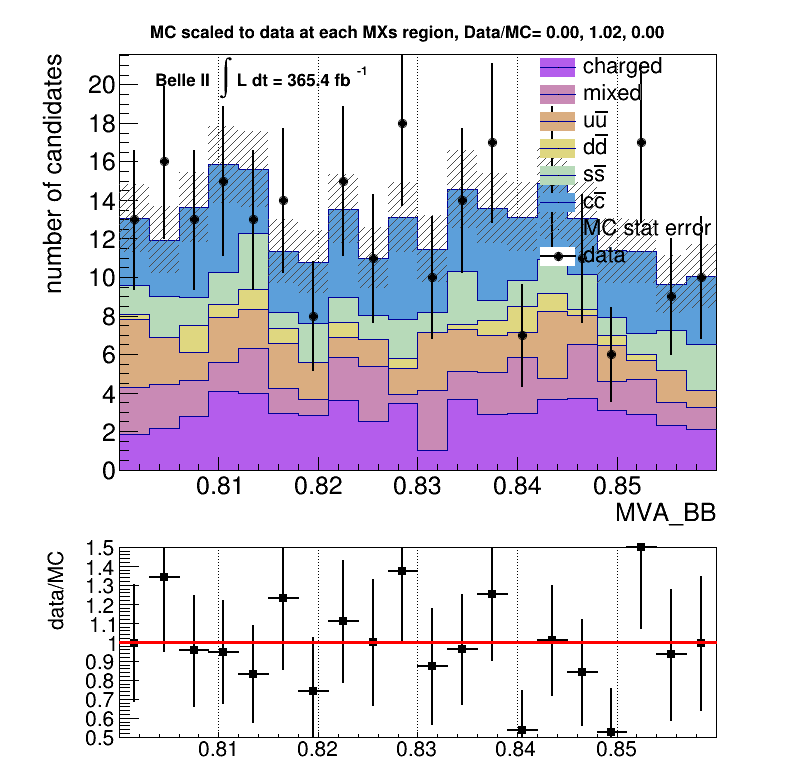
\includegraphics[width=0.3\textwidth]{./picture/FBDT_sideband/MVA_BB_sideband_MXs2.png}}
  \subfloat[][$1.0 \leq M_{X_{s}}^{\textrm{reco}} < 2.0~\textrm{GeV}/c^{2}$]{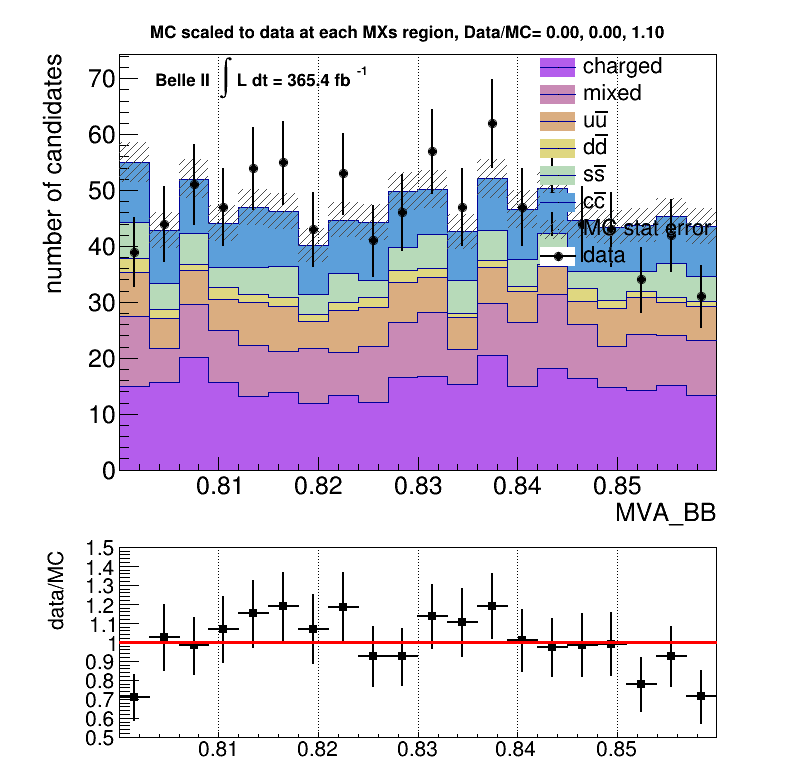
\includegraphics[width=0.3\textwidth]{./picture/FBDT_sideband/MVA_BB_sideband_MXs3.png}}
  \caption{FastBDT output distributions in the FastBDT sideband.}
  \label{fig:FBDT_sideband_distribution}
\end{figure}
The distributions show good agreement between data and MC.
$\chi^{2}$ values are
\begin{equation}
    \chi^{2}_{19} = 
  \begin{cases}
    11.97 & (0.0 < M_{X_{s}}^{\textrm{reco}} < 0.6~\textrm{GeV}/c^{2}), \\[10pt]
    13.41 & (0.6 \leq M_{X_{s}}^{\textrm{reco}} < 1.0~\textrm{GeV}/c^{2}), \\[10pt]
    17.31 & (1.0 \leq M_{X_{s}}^{\textrm{reco}} < 2.0~\textrm{GeV}/c^{2}),
  \end{cases}
\end{equation}
with 19 degrees of freedom.
Here, the number of degrees of freedom is 19 rather than 20 because the MC distributions are normalized to the data in Figure~\ref{fig:FBDT_sideband_distribution}.
Since an overall normalization uncertainty of $\pm20\%$ is assigned to the background samples, only the shape agreement is evaluated.
The corresponding $p$-values are
\begin{equation}
    p\textrm{-value} = 
  \begin{cases}
    \mathcal{P}(\chi^{2}_{19} > 11.97) = 0.89 & (0.0 < M_{X_{s}}^{\textrm{reco}} < 0.6~\textrm{GeV}/c^{2}), \\[10pt]
    \mathcal{P}(\chi^{2}_{19} > 13.41) = 0.82 & (0.6 \leq M_{X_{s}}^{\textrm{reco}} < 1.0~\textrm{GeV}/c^{2}), \\[10pt]
    \mathcal{P}(\chi^{2}_{19} > 17.31) = 0.57 & (1.0 \leq M_{X_{s}}^{\textrm{reco}} < 2.0~\textrm{GeV}/c^{2}),
  \end{cases}
\end{equation}
indicating acceptable agreement between data and MC.

\chapter{Control sample study}
\label{sec:control_sample}
In this analysis, $B\rightarrow X_{s} J/\psi$ is selected as a control sample.
This decay mode has a large branching ratio and contains an $X_{s}$ system.
We use the control sample to estimate the correction factor for the FastBDT output requirement and its uncertainty.

We do not produce $B\rightarrow X_{s} J/\psi$ MC samples separately.
Instead, we extract $B\rightarrow X_{s} J/\psi$ decays from the official $B\bar{B}$ background samples.
The official $B\bar{B}$ background samples contain double counting in some $B\rightarrow X_{s} J/\psi$ decay channels, such as $B^{+} \rightarrow J/\psi K^{+} \pi^{+} \pi^{-}$.
Therefore, we reweight those double-counted decay channels.

The $B\rightarrow X_sJ/\psi$ analysis procedure is similar to that of the $B\rightarrow X_s\nu\bar{\nu}$ analysis.
However, the following additional procedures are applied at the reconstruction stage:
\begin{enumerate}
  \item Reconstruct $B_{\textrm{tag}}$ and $X_{s}$ candidates. The reconstruction method is the same as that used in the $B\rightarrow X_s\nu\bar{\nu}$ analysis described in Section~\ref{sec:reconstruction}.
  \label{item:B_Xs_reco_control}
  \item Reconstruct $J/\psi(\rightarrow\mu^{+}\mu^{-})$. Selection criteria are
  \begin{itemize}
    \item $\mu$: $dr < 2~\textrm{cm}$, $\left| dz \right| < 4~\textrm{cm}$, and $\texttt{muonID} > 0.1$
    \item$J/\psi$: reconstructed from two muons, with the requirement $\left|\Delta M\right|<0.05~\textrm{GeV}/c^{2}$.
  \end{itemize}
  \item Reconstruct $B_{\textrm{sig}}(\rightarrow X_{s}J/\psi)$. Selection criteria are
  \begin{itemize}
    \item $M_{bc} > 5.25~\textrm{GeV}/c^{2}$ and $\left| \Delta E \right| < 0.1~\textrm{GeV}$
  \end{itemize}
  \item Reconstruct $\Upsilon(4S)(\rightarrow B_{\textrm{sig}}B_{\textrm{tag}})$
  \label{item:Upsilon_reco_control}
  \item Perform the BCS for the $J/\psi$ that is a daughter of the reconstructed $\Upsilon(4S)$ candidates in~(\ref{item:Upsilon_reco_control}). Random selection is used for BCS.
  \label{item:BCS_control}
  \item Select the $B_{\textrm{tag}}$ and $X_{s}$ candidates reconstructed in step~\ref{item:B_Xs_reco_control} that do not contain the muons from the $J/\psi$ selected in step~\ref{item:BCS_control}.
  \label{item:selected_B_Xs_control}
  \item Apply the $B\rightarrow X_{s}\nu\bar{\nu}$ analysis procedure using the selected $B_{\textrm{tag}}$ and $X_{s}$ candidates.
  \begin{itemize}
    \item The muons from the $J/\psi$ in step~\ref{item:Upsilon_reco_control} are excluded when calculating the kinematic variables and the $D$-veto information.
  \end{itemize}
\end{enumerate}
Table~\ref{tab:cutflow_Jpsi_1} shows the cut flow for $B\rightarrow X_{s} J/\psi$ MC studies.
\begin{sidewaystable}
\caption{
        Cut flow for the $B\rightarrow X_s J/\psi$ MC study.
        The entries show the numbers of surviving events, except in the
        last column, which shows the data-to-MC ratio.
        The signal and background samples are scaled to an integrated
        luminosity of $365.37~\textrm{fb}^{-1}$.
        Cross-feed events are included in the signal category.
        The calibration and correction factors listed in
        Section~\ref{sec:correction} are not applied.
    }
    \centering
    \renewcommand{\arraystretch}{1.2}
    \setlength{\tabcolsep}{5pt}

    \begin{adjustbox}{max width=0.98\textheight}
    \begin{tabular}{
        l ||
        c | c | c | c | c | c | c || c
    }
        \hline
        \hline

        Selection
        & SIGNAL
        & CHG
        & MIX
        & UUBAR
        & DDBAR
        & SSBAR
        & CHARM
        & data/MC \\
        \hline

        Generated
        & \multicolumn{7}{c||}{$365.37~\textrm{fb}^{-1}$}
        & 1.0000 \\

        Skim
        & $2.71\times10^{5}$
        & $3.42\times10^{7}$
        & $2.60\times10^{7}$
        & $9.11\times10^{7}$
        & $2.19\times10^{7}$
        & $1.73\times10^{7}$
        & $9.64\times10^{7}$
        & 1.0475 \\

        Reconstruction and preselections
        & 368.6
        & 1.0
        & 0.8
        & 6.8
        & 0.8
        & 1.3
        & 3.8
        & 0.6398 \\

        $M_{\textrm{bc}}>5.27~\textrm{GeV}/c^{2}$ for $B_{\textrm{tag}}$
        & 332.3
        & 0.8
        & 0.8
        & 3.0
        & 0.3
        & 0.5
        & 1.5
        & 0.6282 \\

        $\left|\Delta E\right|<0.2~\textrm{GeV}$ for $B_{\textrm{tag}}$
        & 310.0
        & 0.8
        & 0.8
        & 2.3
        & 0.3
        & 0.5
        & 0.8
        & 0.6026 \\

        $E_{\textrm{ecl}}<1.3~\textrm{GeV}$
        & 308.0
        & 0.8
        & 0.8
        & 2.3
        & 0.3
        & 0.5
        & 0.8
        & 0.6065 \\

        $17^\circ < \theta_{\textrm{missing}} < 150^\circ$
        & 295.3
        & 0.8
        & 0.8
        & 1.8
        & 0.3
        & 0.5
        & 0.8
        & 0.6100 \\

        $0.5<p_{X_{s}}^{*}<2.96~\textrm{GeV}/c$
        & 295.3
        & 0.8
        & 0.8
        & 1.8
        & 0.3
        & 0.5
        & 0.8
        & 0.6100 \\

        Reject
        $1.84<M_{X_{s}}^{\textrm{reco}}<1.89~\textrm{GeV}/c^{2}$
        & 292.5
        & 0.8
        & 0.8
        & 1.8
        & 0.3
        & 0.5
        & 0.8
        & 0.6055 \\

        BCS
        & 292.5
        & 0.8
        & 0.8
        & 1.8
        & 0.3
        & 0.5
        & 0.8
        & 0.6055 \\

        $\mathcal{O}_{\textrm{BDT}}>0.86$
        & 219.6
        & 0.3
        & 0.3
        & 0.3
        & 0
        & 0
        & 0
        & 0.6262 \\

        \hline
        \hline
    \end{tabular}
    \end{adjustbox}
    \label{tab:cutflow_Jpsi_1}
\end{sidewaystable}

Figure~\ref{fig:Jpsi_plot} shows the distributions of the $J/\psi$ mass difference $\Delta M$, $M_{\textrm{bc}}$, and $\Delta E$.
These distributions are obtained after the BCS of the $\Upsilon(4S)$ candidates.
\begin{figure}
    \centering
    \subfloat[][$\Delta M$ of $J/\psi$]{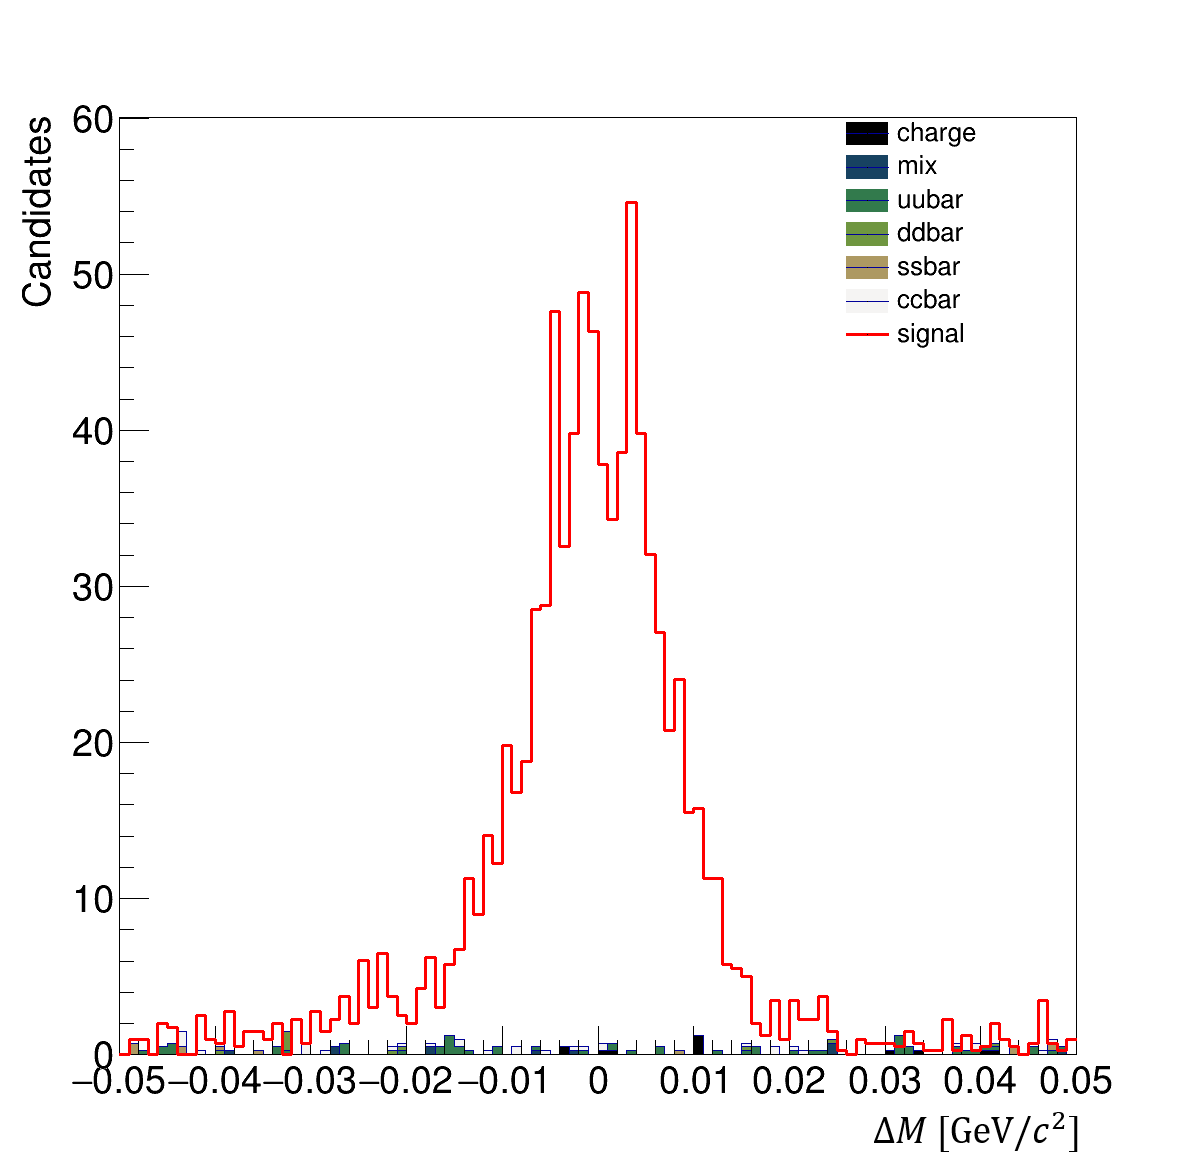
\includegraphics[width=0.3\textwidth]{./picture/XsJpsi/Plot_dM_Jpsi.png}}
    \subfloat[][$M_{\textrm{bc}}$ of $B_{\textrm{sig}}$]{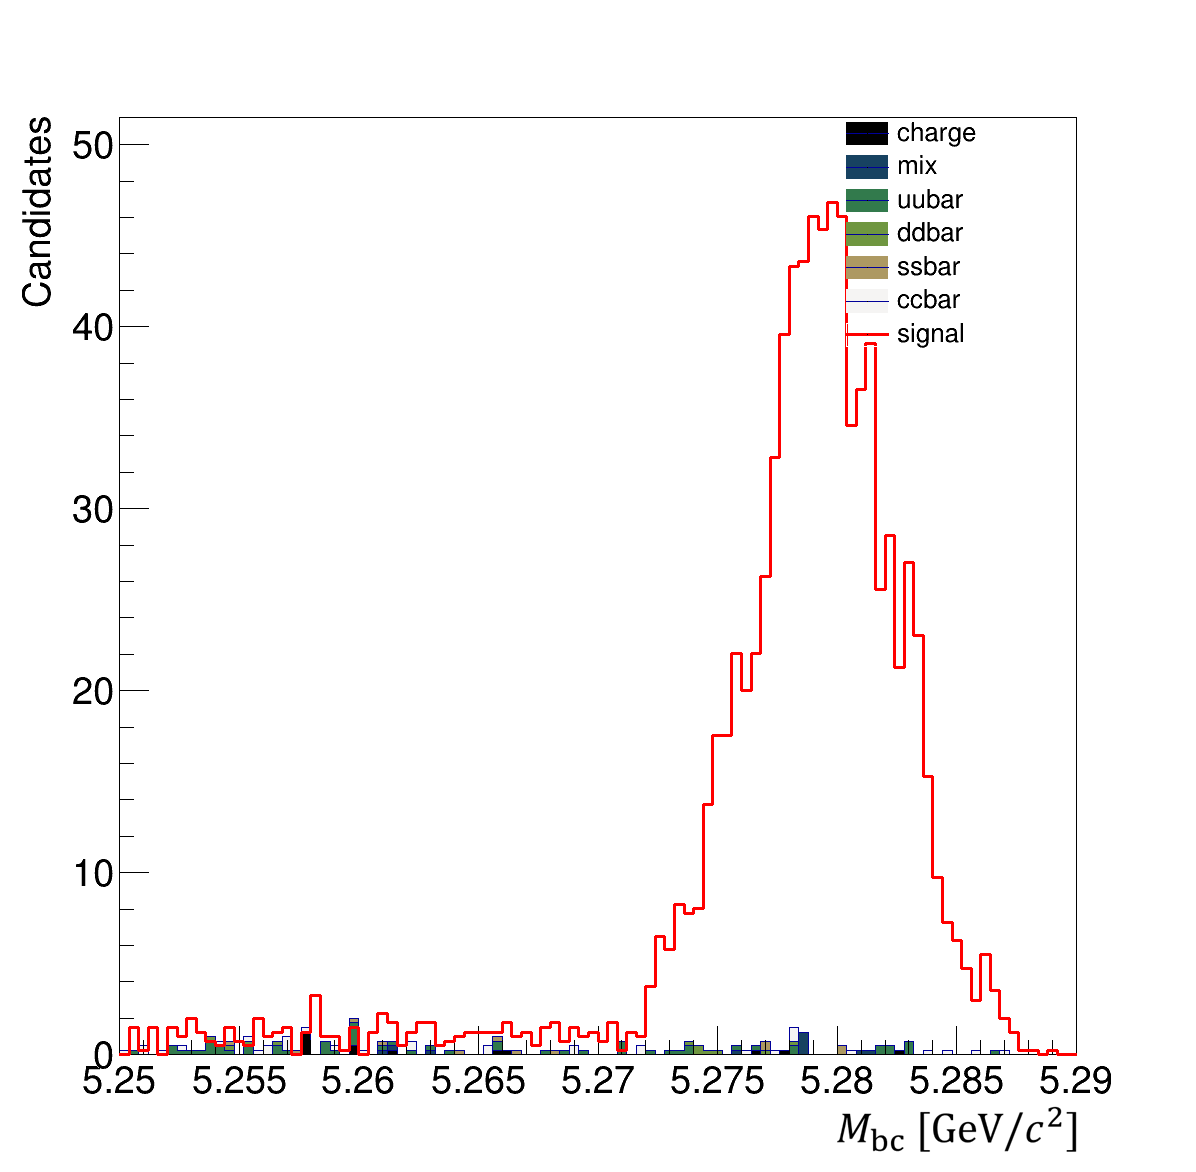
\includegraphics[width=0.3\textwidth]{./picture/XsJpsi/Plot_Mbc_Jpsi.png}}
    \subfloat[][$\Delta E$ of $B_{\textrm{sig}}$]{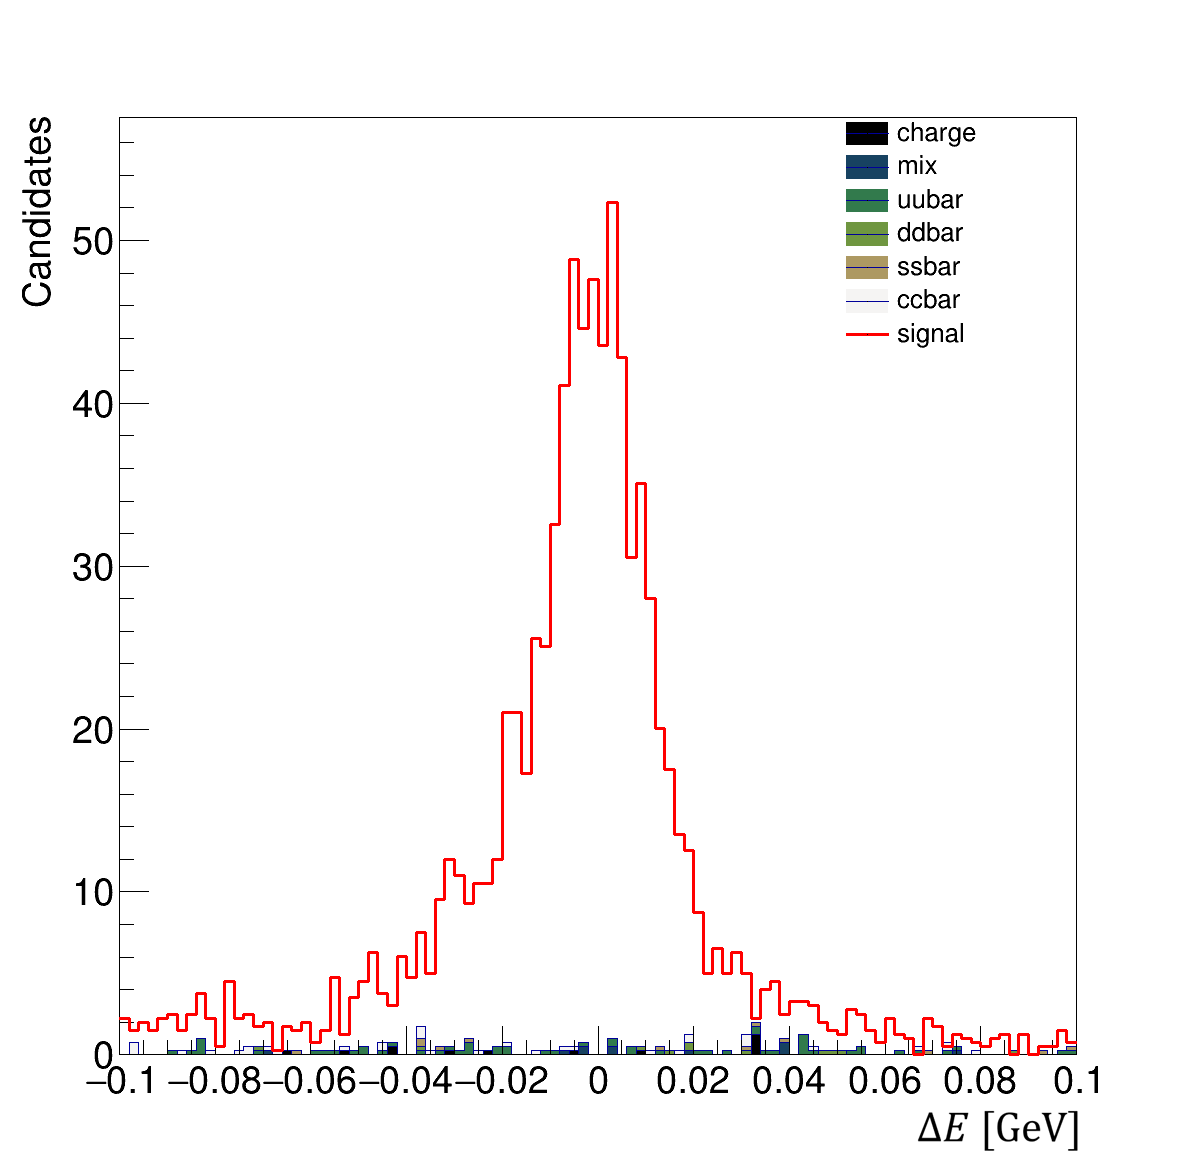
\includegraphics[width=0.3\textwidth]{./picture/XsJpsi/Plot_delE_Jpsi.png}}
    \caption{Distributions of variables for $B\rightarrow X_{s} J/\psi$ analysis. $\Delta M$ distribution is for $J/\psi$ which is a granddaughter of $\Upsilon(4S)$ candidates. The $M_{\textrm{bc}}$ and $\Delta E$ distributions are for $B_{sig}$ that is a daughter of $\Upsilon(4S)$ candidates. These plots are made after BCS of $\Upsilon(4S)$.}
    \label{fig:Jpsi_plot}
\end{figure}

Figure~\ref{fig:FBDT_control_without_signal_embedding} shows the FastBDT output distribution for $B\rightarrow X_{s} J/\psi$ analysis.
The third bin in the right figure shows a large discrepancy between data and MC.
This large discrepancy had not been found in the previous iteration.
In Appendix~\ref{sec:Jpsi_third_bin}, this discrepancy is investigated.
We conclude that this large deviation can occur when the look-elsewhere effect associated with FastBDT retraining is taken into account.
Figures~\ref{fig:XsJpsi_used_vars1}--\ref{fig:XsJpsi_used_vars2} show the distributions of the FastBDT input variables.
The MC distributions are normalized to the data in Figures~\ref{fig:XsJpsi_used_vars1}--\ref{fig:XsJpsi_used_vars2}.
\begin{figure}
    \centering
    \subfloat{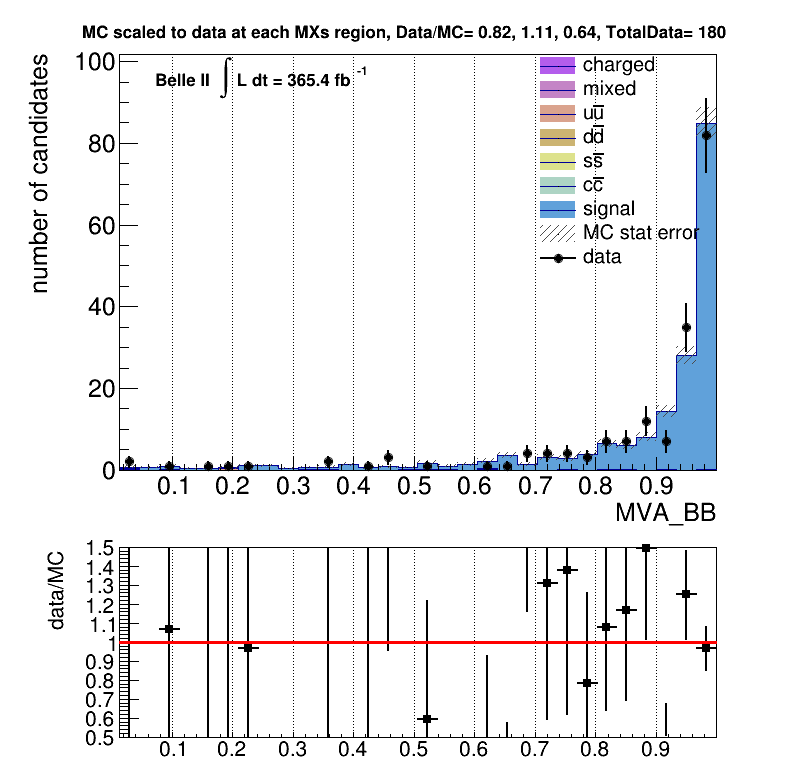
\includegraphics[width=0.5\textwidth]{./picture/XsJpsi/MVA_BB_Jpsi.png}}
    \subfloat{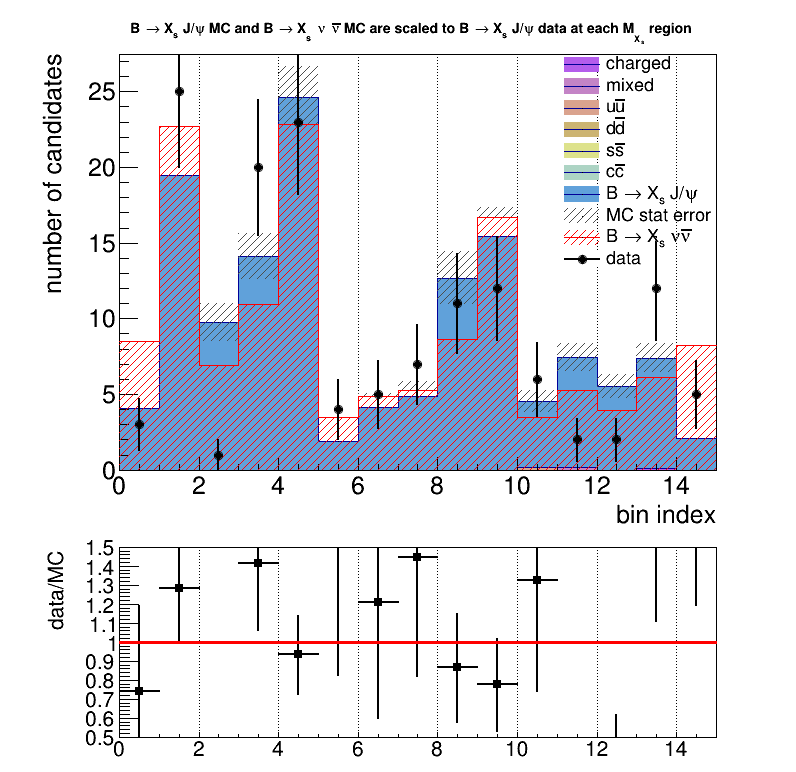
\includegraphics[width=0.5\textwidth]{./picture/XsJpsi/bin_index_Jpsi_compare.png}}
    \caption{The left plot shows the FastBDT output distribution for $B\rightarrow X_{s} J/\psi$ analysis. The right plot shows the bin index distribution defined in Section~\ref{subsec:histogram_templates}. In both plots, calibration and correction factors in Section~\ref{sec:correction} are applied, except for the $q\bar q$ correction factor. For the comparison, the right plot also includes the $B\rightarrow X_s\nu\bar{\nu}$ signal MC distribution for comparison.}
    \label{fig:FBDT_control_without_signal_embedding}
\end{figure}

The data-to-MC ratios are
\begin{equation}
    \frac{N_{Data}}{N_{MC}} = 
  \begin{cases}
    0.82 \pm 0.10 & (0.0 < M_{X_{s}}^{\textrm{reco}} < 0.6~\textrm{GeV}), \\[10pt]
    1.17 \pm 0.21 & (0.6 \leq M_{X_{s}}^{\textrm{reco}} < 1.0~\textrm{GeV}), \\[10pt]
    0.61 \pm 0.12 & (1.0 \leq M_{X_{s}}^{\textrm{reco}} < 2.0~\textrm{GeV}),
  \end{cases}
\end{equation}
where only the statistical uncertainties in data and MC are included.
The calibration and correction factors listed in Section~\ref{sec:correction} are applied, except for the $q\bar q$ correction factor.

For the FastBDT selection efficiency, the data-to-MC ratios are
\begin{equation}
      \label{eq:FBDT_efficiency_ratio_data_MC_XsJpsi}
      \frac{\epsilon_{Data}^{FBDT}}{\epsilon_{MC}^{FBDT}} = 
    \begin{cases}
      1.00 \pm 0.04 & (0.0 < M_{X_{s}}^{\textrm{reco}} < 0.6~\textrm{GeV}/c^{2}), \\[10pt]
      1.05 \pm 0.08 & (0.6 \leq M_{X_{s}}^{\textrm{reco}} < 1.0~\textrm{GeV}/c^{2}), \\[10pt]
      0.97 \pm 0.14 & (1.0 \leq M_{X_{s}}^{\textrm{reco}} < 2.0~\textrm{GeV}/c^{2}),
    \end{cases}
\end{equation}
where $\epsilon_{\textrm{Data}}^{\textrm{FBDT}}$ and $\epsilon_{\textrm{MC}}^{\textrm{FBDT}}$ are the FastBDT selection efficiencies in data and MC, respectively.

\chapter{Calibration and corrections}
\label{sec:correction}
\section{Hadron PID}
\label{sec:pid_correction}
In this analysis, we apply corrections to the hadron PID efficiencies in the MC samples.
These correction factors are calculated in the two-dimensional plane of momentum and polar angle.

For the kaon and pion efficiencies, we use the Belle II systematic framework with the $D^{*+}\rightarrow D^{0}(\rightarrow K^{-}\pi^{+})\pi^{+}$ decay mode~\cite{Belle-II:2025tpe}.
The kaon--pion misidentification rates are also corrected..
Figures~\ref{fig:KaonEff} and~\ref{fig:PionEff} show the data-to-MC ratio for the kaon and pion PID efficiencies.
Figure~\ref{fig:Kaonmis} shows the data-to-MC ratio for the misidentification rate for pions identified as kaons.
Figure~\ref{fig:Pionmis} shows the data-to-MC ratio for the misidentification rate for kaons identified as pions.

Leptons misidentified as kaons or pions constitute one source of background.
In Section~\ref{sec:PID_fakes}, the particle compositions of the kaon and pion candidates are shown.
We correct the rates at which electrons and muons are misidentified as pions or kaons.
Figures~\ref{fig:KaonEplus} and~\ref{fig:KaonEminus} show the data-to-MC ratios for the rates at which electrons are misidentified as kaons.
Figures~\ref{fig:KaonMUplus} and~\ref{fig:KaonMUminus} show the data-to-MC ratios for the rates at which muons are misidentified as kaons.
Figures~\ref{fig:PionEplus} and~\ref{fig:PionEminus} show the data-to-MC ratios for the rates at which electrons are misidentified as pions.
Figures~\ref{fig:PionMUplus} and~\ref{fig:PionMUminus} show the data-to-MC ratios for the rates at which muons are misidentified as pions.

If a PID correction factor has an unphysical value, the correction is not applied.
Figure~\ref{fig:PID_unphysical} shows the ratio of events for which the PID correction factor has an unphysical value in the signal sample.
In addition, if the momentum or polar angle lies outside the calibrated range, the correction is not applied.
\begin{figure}
  \centering
  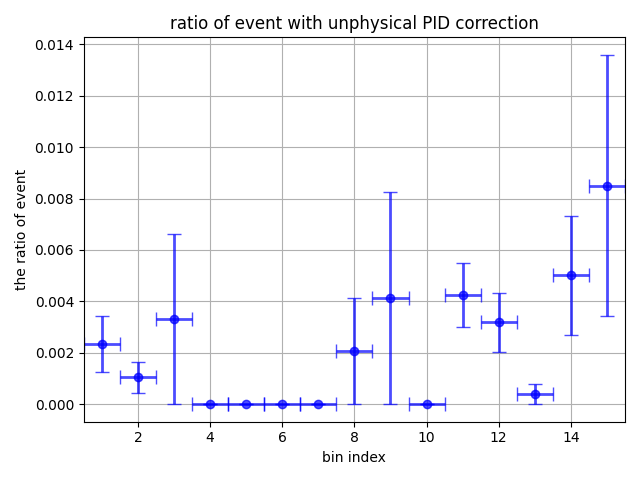
\includegraphics[width=0.5\textwidth]{./picture/systematic/check_PID_ratio.png}
  \caption{The ratio of events whose PID correction is unphysical}
  \label{fig:PID_unphysical}
\end{figure}

\section{Photon multiplicity}
\label{sec:photon_mul_corr}
It is known that the Belle II simulation does not model the beam background perfectly.
To address this issue, an ECL energy-scale correction~\cite{Belle-II:2024ami} or a photon-multiplicity correction~\cite{Belle-II:2023esi} is applied in other analyses.
In this analysis, a photon-multiplicity correction is applied.
To determine the photon-multiplicity correction factor, two wrong-charge sidebands are defined.
The wrong-charge sidebands are defined by reconstructing $\Upsilon(4S)$ with an incorrect charge combination of $B_{\textrm{tag}}$ and $X_{s}$:
\begin{itemize}
  \item Neutral-signal wrong-charge sideband: $\Upsilon(4S)$ is reconstructed from $B^{\pm}_{\textrm{tag}} X_{sd}^{0}$.
  \item Neutral-tag wrong-charge sideband: $\Upsilon(4S)$ is reconstructed from $B^{0}_{\textrm{tag}} X_{su}^{\pm}$.
\end{itemize}
The photon multiplicity correction factor is obtained from the neutral-signal wrong-charge sideband.
The neutral-tag wrong-charge sideband is used to validate the photon multiplicity correction and estimate its uncertainty.

The multiplicity of the remaining photon candidates is examined.
The correction factor for the photon multiplicity is obtained by
\begin{equation}
    C_{i} = \frac{N_{i}^{data}}{N_{i}^{MC}} \times \frac{\sum N_{j}^{MC}}{\sum N_{j}^{data}},
\end{equation}
where $C_{i}$ is the correction factor, $N_{i}^{data}$ is the number of events in data, and $N_{i}^{MC}$ is the number of events in MC when the number of remaining photon candidates is $i$.

Figure~\ref{fig:neutral_signal_wrong_charge_side} shows the distribution of the number of remaining photon candidates for the neutral-signal wrong-charge sideband.
The left plot shows the distribution before the photon multiplicity correction.
The right plot shows the distribution after the correction.
\begin{figure}
  \centering
  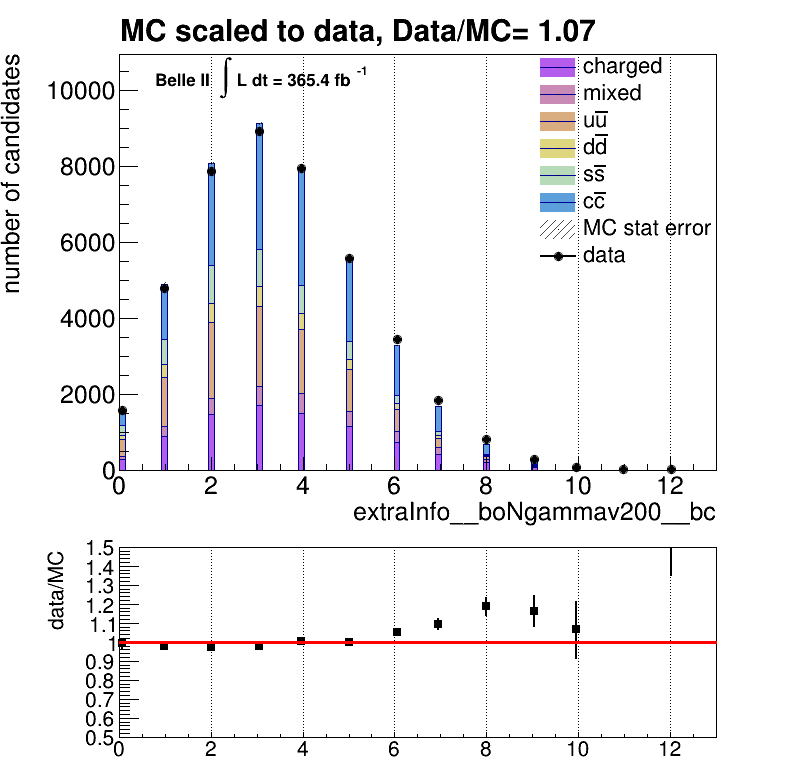
\includegraphics[width=0.45\textwidth]{./picture/neutral_signal_wrong_charge_sideband/extraInfo__boNgammav200__bc_sideband.png}
  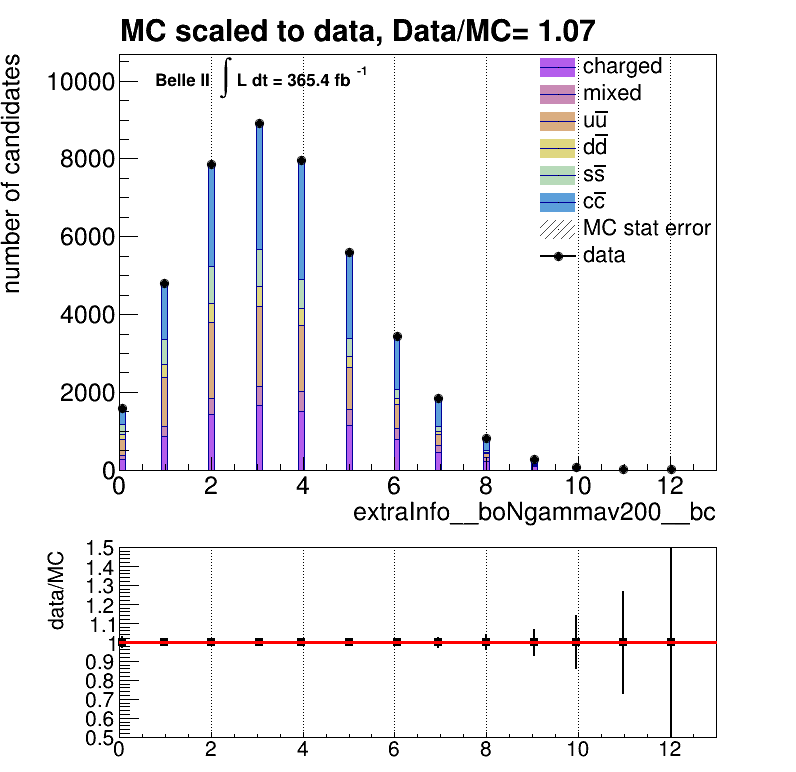
\includegraphics[width=0.45\textwidth]{./picture/neutral_signal_wrong_charge_sideband_correction/extraInfo__boNgammav200__bc_sideband.png}
  \caption{Distribution of the number of remaining photon candidates in the neutral-signal wrong-charge sideband. The left plot shows the distribution before the photon-multiplicity correction, and the right plot shows the distribution after the correction. By definition, the data-to-MC ratio is unity in each photon-multiplicity bin after the correction.}
  \label{fig:neutral_signal_wrong_charge_side}
\end{figure}

Figure~\ref{fig:neutral_tag_wrong_charge_sideband} shows the distribution of the number of remaining photon candidates for the neutral-tag wrong-charge sideband.
After the correction, the data-MC agreement improves, especially in the high-photon-multiplicity region.
\begin{figure}
  \centering
  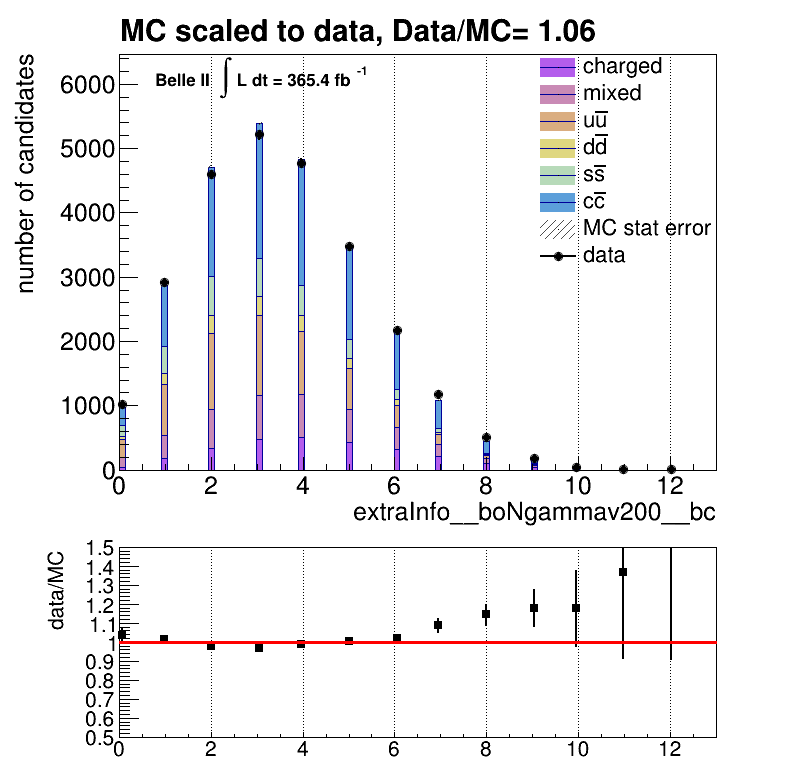
\includegraphics[width=0.45\textwidth]{./picture/neutral_tag_wrong_charge_sideband/extraInfo__boNgammav200__bc_sideband.png}
  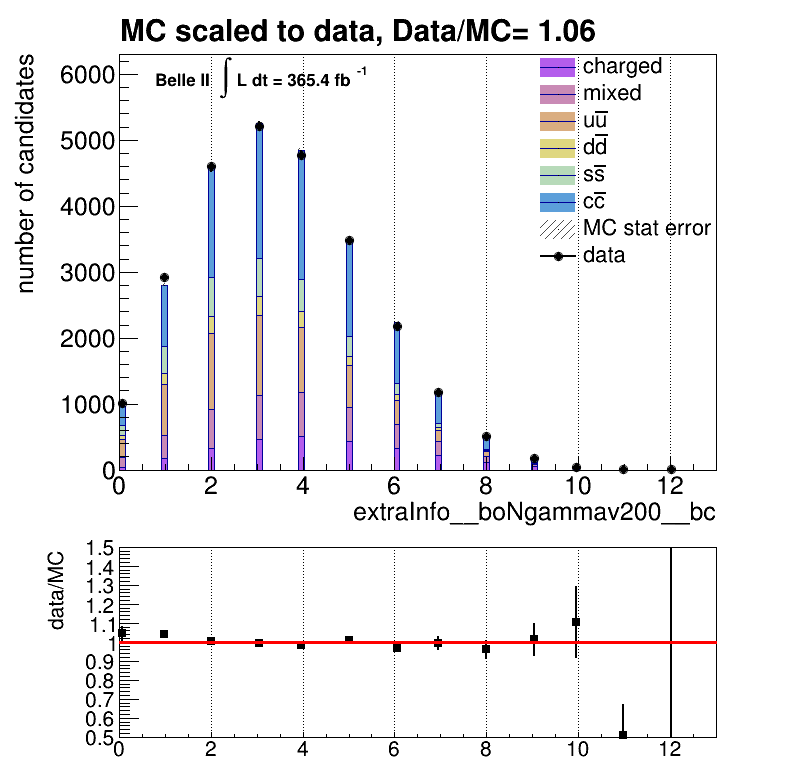
\includegraphics[width=0.45\textwidth]{./picture/neutral_tag_wrong_charge_sideband_correction/extraInfo__boNgammav200__bc_sideband.png}
  \caption{Distribution of the number of remaining photon candidates in the neutral-tag wrong-charge sideband. The left plot shows the distribution before the photon-multiplicity correction, and the right plot shows the distribution after the correction. The data-to-MC ratio is not exactly unity after the correction. These residual data-to-MC differences are used to estimate the systematic uncertainty associated with the photon-multiplicity correction.}
  \label{fig:neutral_tag_wrong_charge_sideband}
\end{figure}

\section{$\pi^{0}$ efficiency}
\label{sec:pi0_eff_corr}
The official correction factor for the $\pi^{0}$ efficiency is applied.
The correction factor is derived from $\tau \rightarrow h\pi^{0}\nu$ decays.
This factor depends on the $\pi^{0}$ momentum and polar angle.
Figure~\ref{fig:pi0_corr_table} shows the $\pi^{0}$ efficiency correction factors.
\begin{figure}[h]
  \centering
  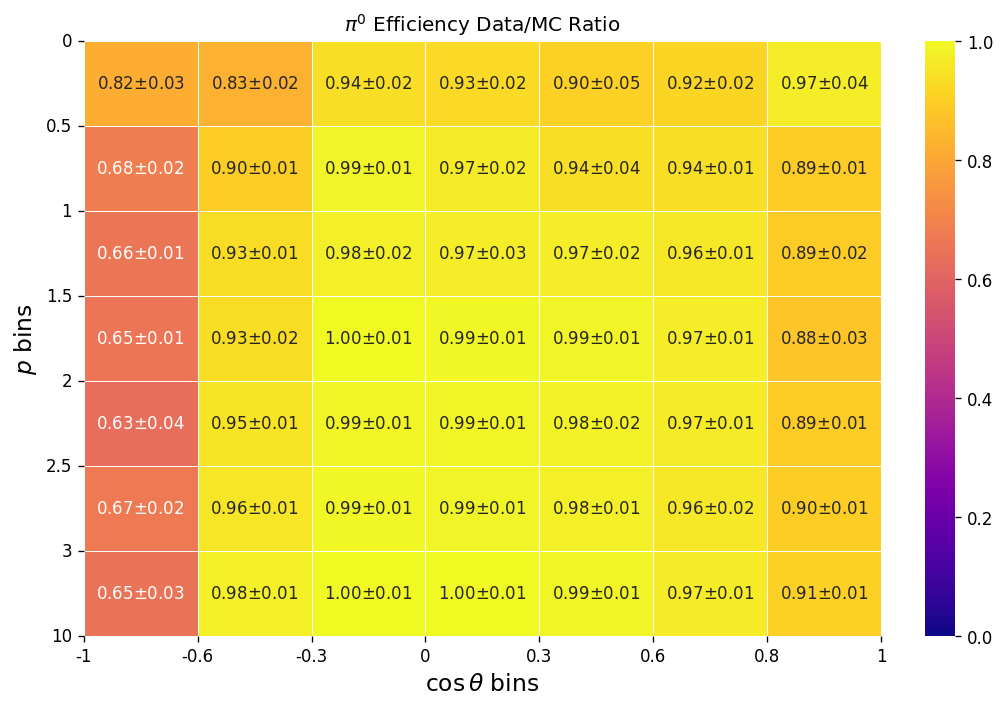
\includegraphics[width=0.5\textwidth]{./picture/systematic/pi0eff30cor.png}
  \caption{Data-to-MC ratio for the $\pi^{0}$ reconstruction efficiency as a function of momentum and polar angle.}
  \label{fig:pi0_corr_table}
\end{figure}

\section{$K_{S}^{0}$ efficiency}
\label{sec:KS0_eff_corr}
The official correction factor for the $K_{S}^{0}$ efficiency is applied.
The correction factor is derived using the $D^{*+} \rightarrow D^{0}(\rightarrow K_{S}^{0}\pi^{+}\pi^{-})\pi^{+}$ decay mode.
This correction factor depends on the $K_{S}^{0}$ momentum, polar angle, and the distance between the IP and the $K_{S}^{0}$ decay vertex.

\section{FastBDT efficiency}
The FastBDT efficiency correction factors are obtained from the $B \rightarrow X_{s} J/\psi$ control-sample study described in Section~\ref{sec:control_sample}.
The data-to-MC ratios given in Eq.~\ref{eq:FBDT_efficiency_ratio_data_MC_XsJpsi} are applied separately in each $M_{X_{s}}^{\textrm{reco}}$ bin.

\section{FEI calibration for $B\bar{B}$}
\label{sec:FEI_calibration}
The official calibration factors for the hadronic FEI efficiency are applied.
The calibration factors are obtained using inclusive $B \rightarrow X\ell\nu$ decays, where $\ell=e$ or $\mu$.
They are determined separately for charged and neutral $B_{\textrm{tag}}$ candidates and for several $B_{\textrm{tag}}$ decay modes.
Figure~\ref{fig:FEIcalibration} shows the FEI calibration factors obtained with the requirement $\mathcal{P}_{\textrm{FEI}}>0.001$.
The labels $e$ and $\mu$ denote the calibration results obtained using the $B \rightarrow Xe\nu$ and $B \rightarrow X\mu\nu$ samples, respectively.
\begin{figure}
  \centering
  \subfloat[][FEI calibration factors for charged $B_{\textrm{tag}}$ candidates.]{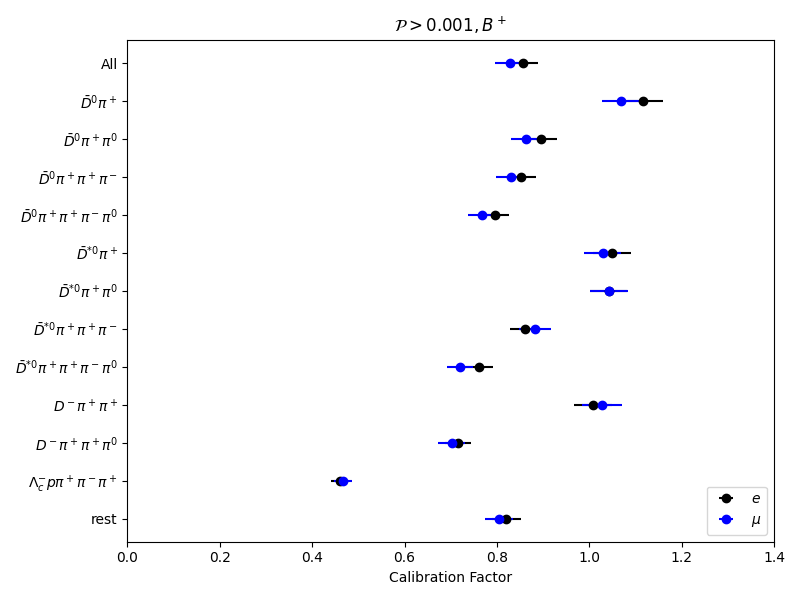
\includegraphics[width=0.45\textwidth]{./picture/systematic/FEI_cal_Bp.png}}
  \hfill
  \subfloat[][FEI calibration factors for neutral $B_{\textrm{tag}}$ candidates.]{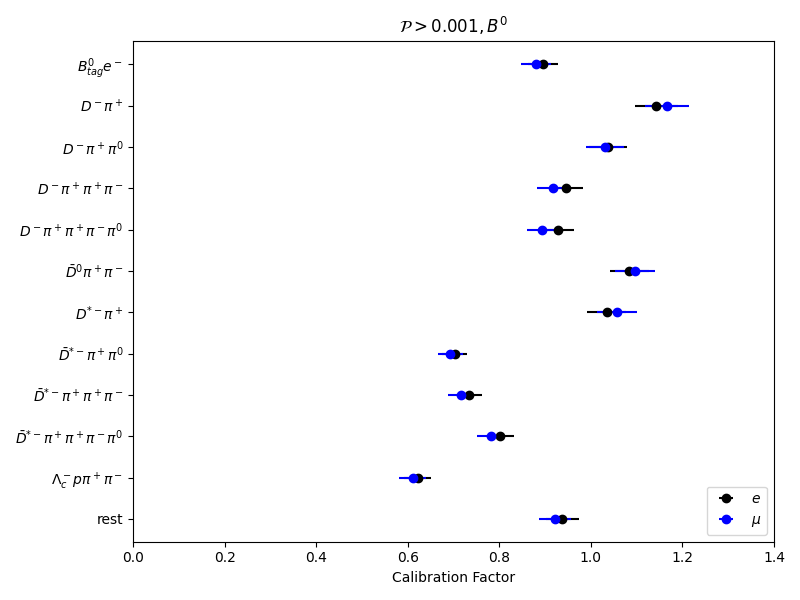
\includegraphics[width=0.45\textwidth]{./picture/systematic/FEI_cal_B0.png}}
  \caption{FEI efficiency calibration factors obtained with the requirement $\mathcal{P}_{\textrm{FEI}}>0.001$. The black and blue points show the results obtained using the $B \rightarrow Xe\nu$ and $B \rightarrow X\mu\nu$ samples, respectively.}
  \label{fig:FEIcalibration}
\end{figure}

\section{$q\bar{q}$ efficiency}
The $q\bar{q}$ background efficiency is corrected using correction factors derived from the off-resonance sample described in Section~\ref{sec:off_resonance}.
The data-to-MC ratios given in Eq.~\ref{eq:off_resonance_ratio} are applied separately in each $M_{X_{s}}^{\textrm{reco}}$ bin.

\section{Fragmentation of $X_{s}$}
\label{sec:frag_corr}
The fragmentation of $X_{s}$ is simulated using \textsc{Pythia8}.
The relative fractions of the decay modes should be corrected using experimental measurements.

Three possible samples are considered for the correction:
\begin{enumerate}
  \item $B \rightarrow X_{s} \ell \bar{\ell}$
  \item $B \rightarrow X_{s} \gamma$
  \item $B \rightarrow X_{s} J/\psi$
\end{enumerate}
Each sample has advantages and disadvantages:
\begin{itemize}
  \item The $B \rightarrow X_{s} \ell \bar{\ell}$ decay is the most similar to the $B \rightarrow X_{s} \nu \bar{\nu}$ decay.
  However, no sufficiently precise measurement is available to derive the correction factors.
  
  \item The $B \rightarrow X_{s} \gamma$ decay proceeds through a similar electroweak-penguin process.
  However, because the photon is a massless spin-1 particle, the spin of the $X_{s}$ system cannot be zero.
  Therefore, the fragmentation may differ from that in $B \rightarrow X_{s} \nu \bar{\nu}$ decays.
  
  \item The $B \rightarrow X_{s} J/\psi$ decay proceeds through a different process dominated by strong interactions.
  Therefore, its fragmentation may also differ from that in $B \rightarrow X_{s} \nu \bar{\nu}$ decays.
\end{itemize}
In this analysis, the fragmentation of the remaining $B \rightarrow X_{s} \nu \bar{\nu}$ signal MC sample, defined in Section~\ref{subsec:signal_MC}, is corrected using the results of the $B \rightarrow X_{s} \gamma$ study.
The uncertainty in this correction is estimated from the difference between the results of the $B \rightarrow X_{s} \gamma$ and $B \rightarrow X_{s} J/\psi$ studies.

Figure~\ref{fig:fragmentation_Xs} shows the fragmentation fractions of the nine decay-mode categories in each $M_{X_{s}}$ region.
The fractions are normalized within these nine categories, and therefore their sum is 100\%.
The blue points show the results of the $B \rightarrow X_{s} \gamma$ study~\cite{Belle:2018iff,Belle:Xsgamma}.
The orange points show the fragmentation fractions in the $B \rightarrow X_{s} \nu \bar{\nu}$ signal MC sample.
Correction factors are derived and applied so that the fragmentation fractions in the $B \rightarrow X_{s} \nu \bar{\nu}$ signal MC sample reproduce those measured in the $B \rightarrow X_{s} \gamma$ study.
The correction factors are not applied in the regions $M_{X_{s}} < 1.15~\textrm{GeV}/c^{2}$ and $M_{X_{s}} > 2.4~\textrm{GeV}/c^{2}$.
\begin{figure}
  \centering
  \subfloat[][]{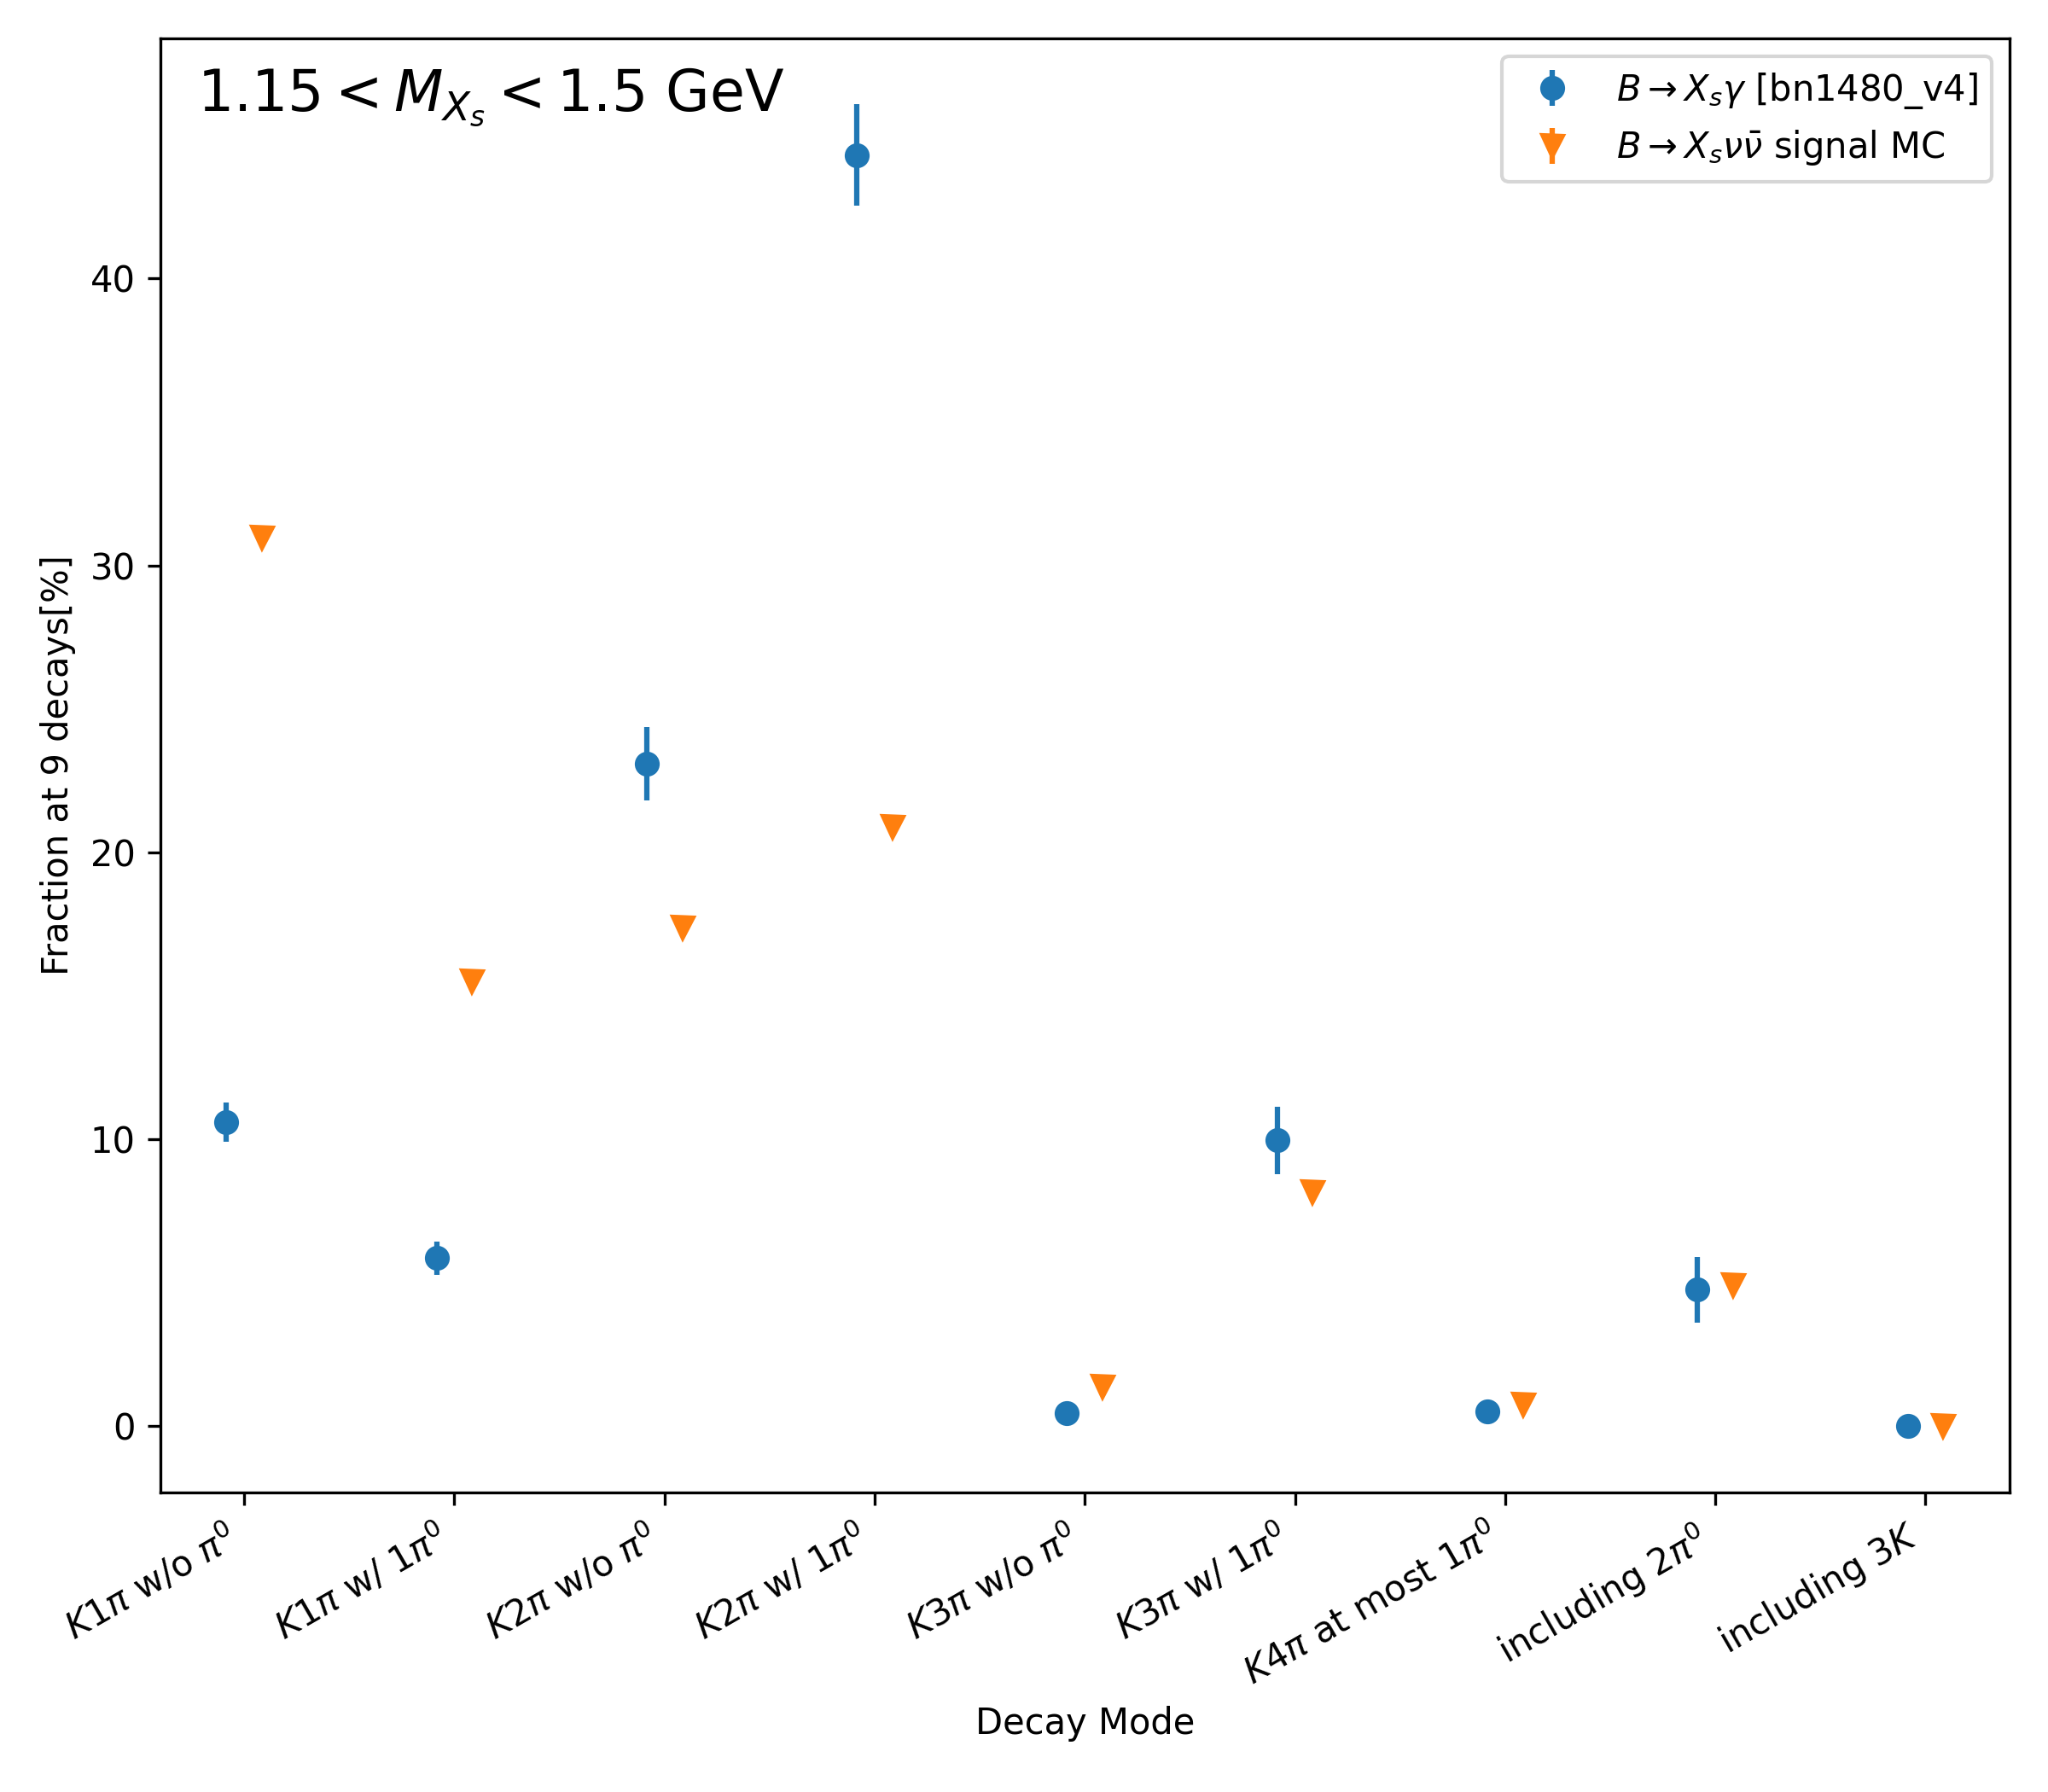
\includegraphics[width=0.32\textwidth]{./picture/systematic/fraction_1.15_1.5.png}}
  \subfloat[][]{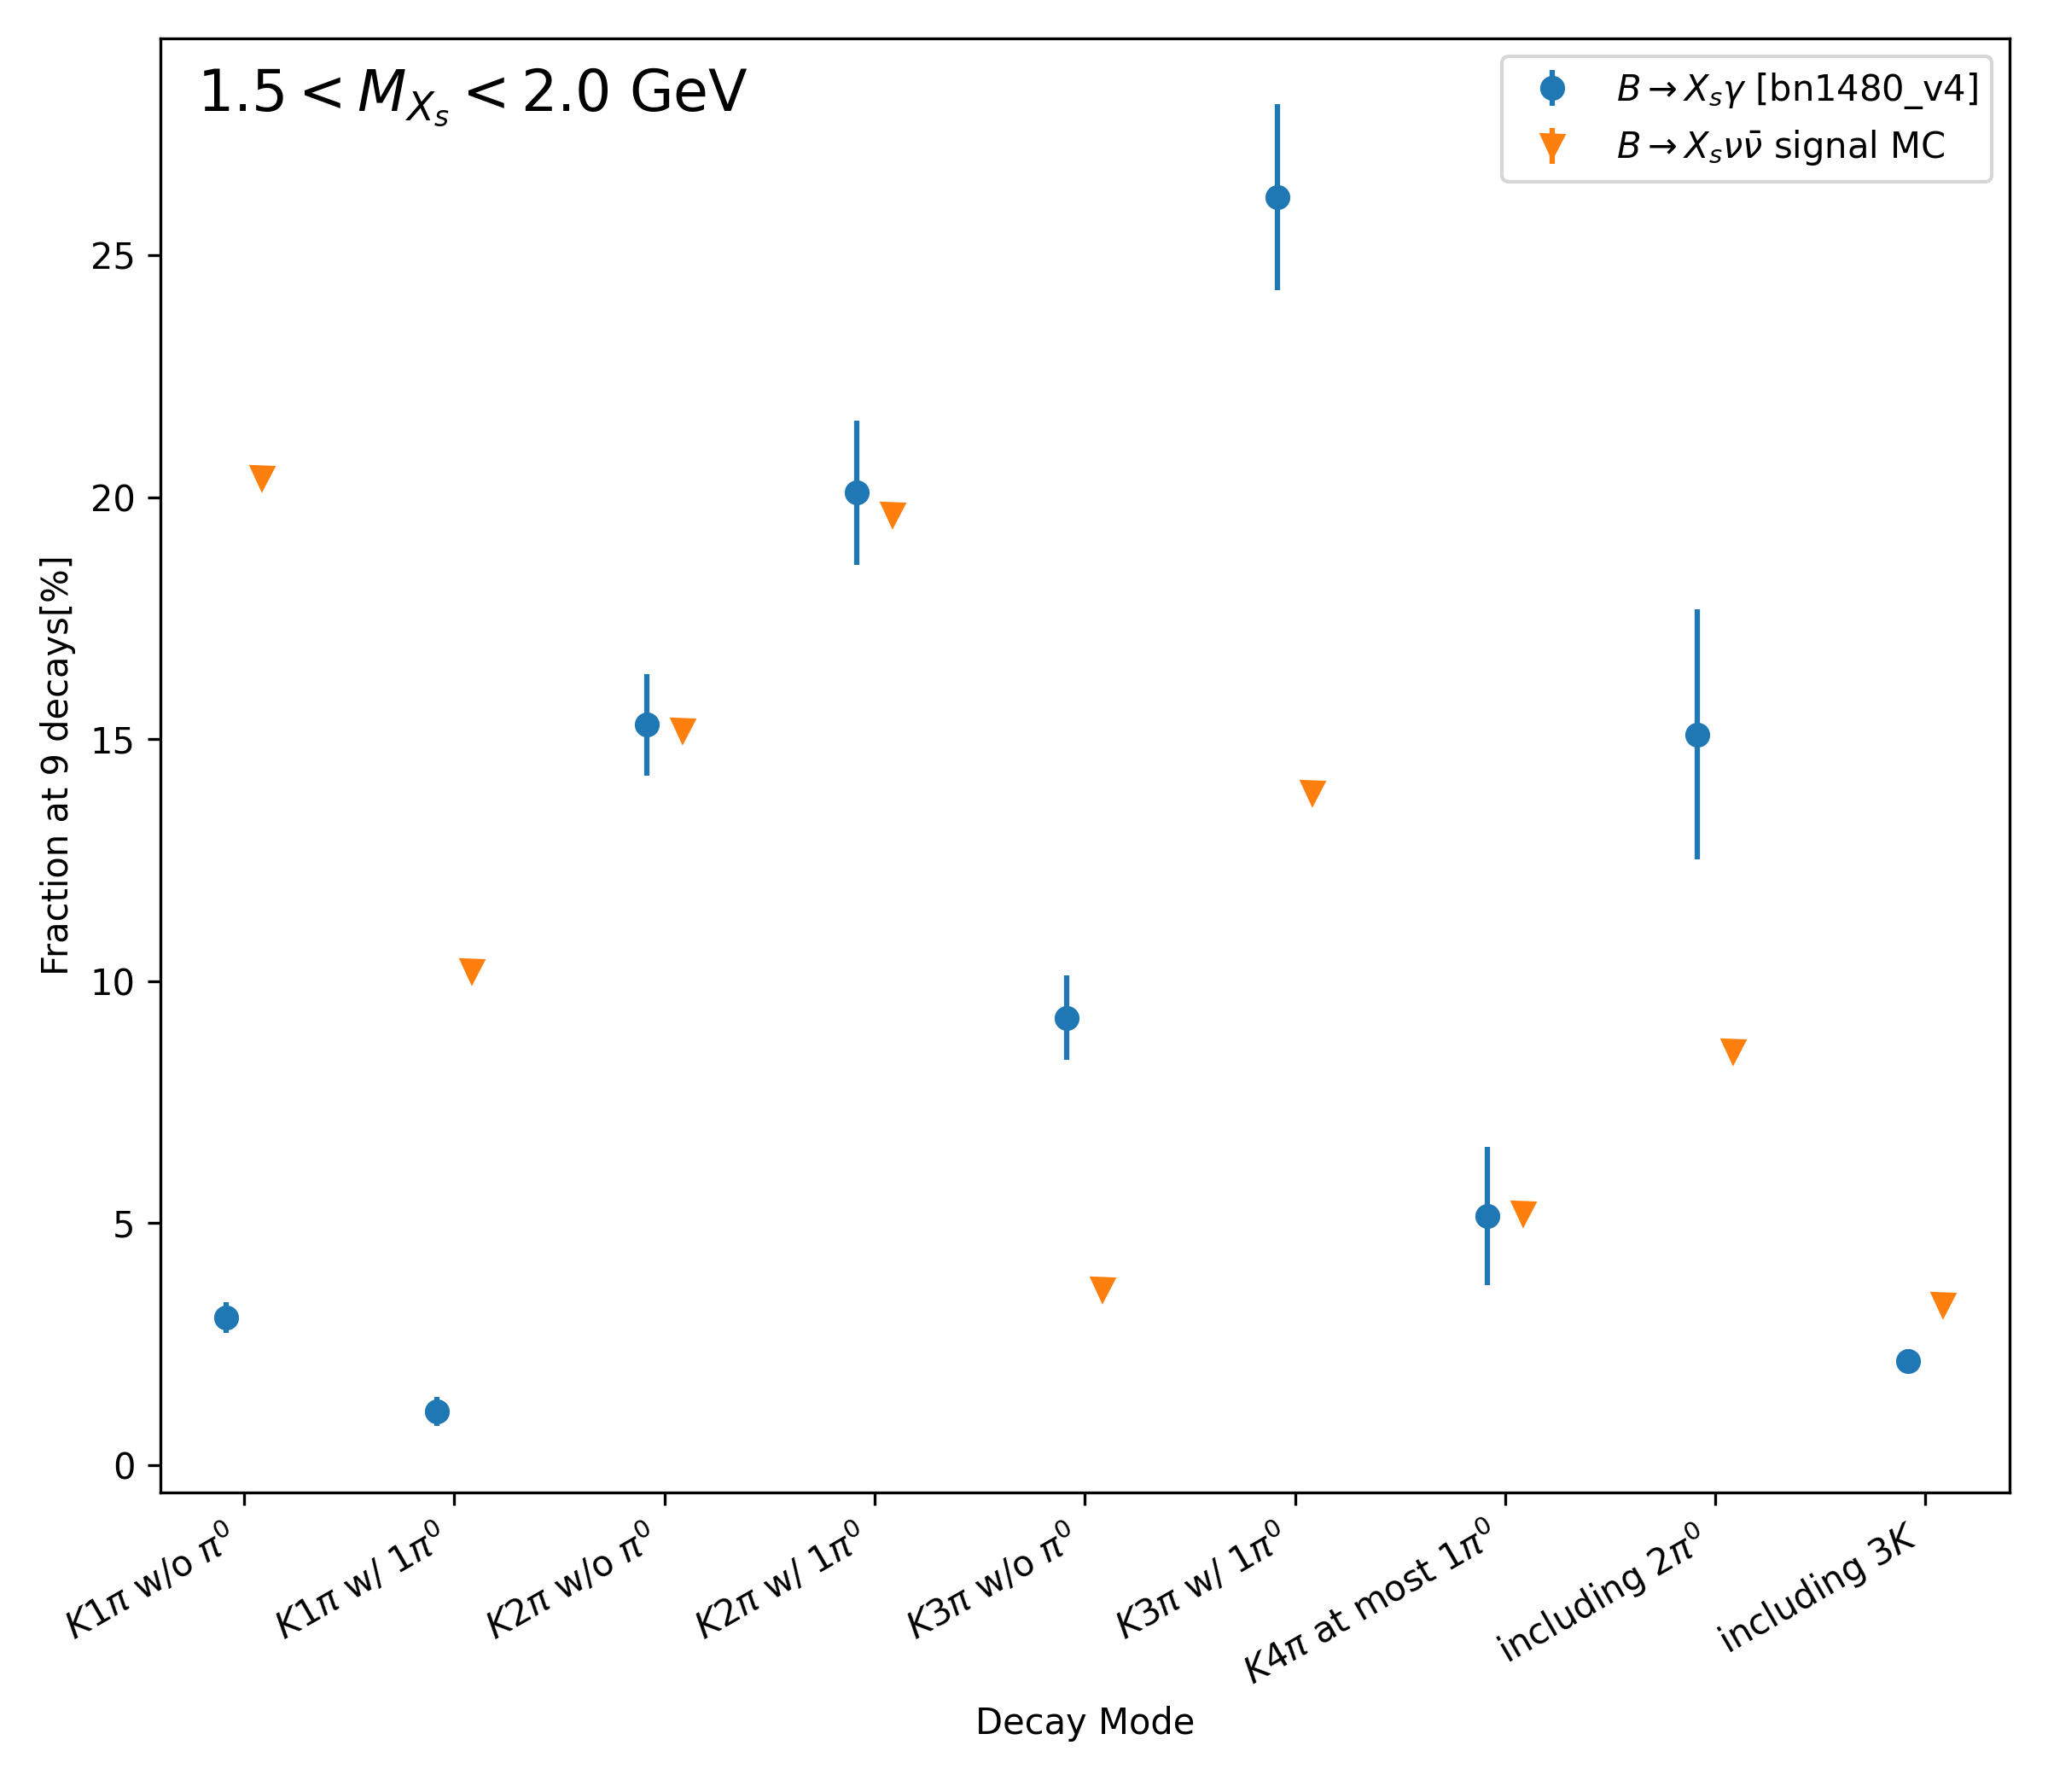
\includegraphics[width=0.32\textwidth]{./picture/systematic/fraction_1.5_2.0.png}}
  \subfloat[][]{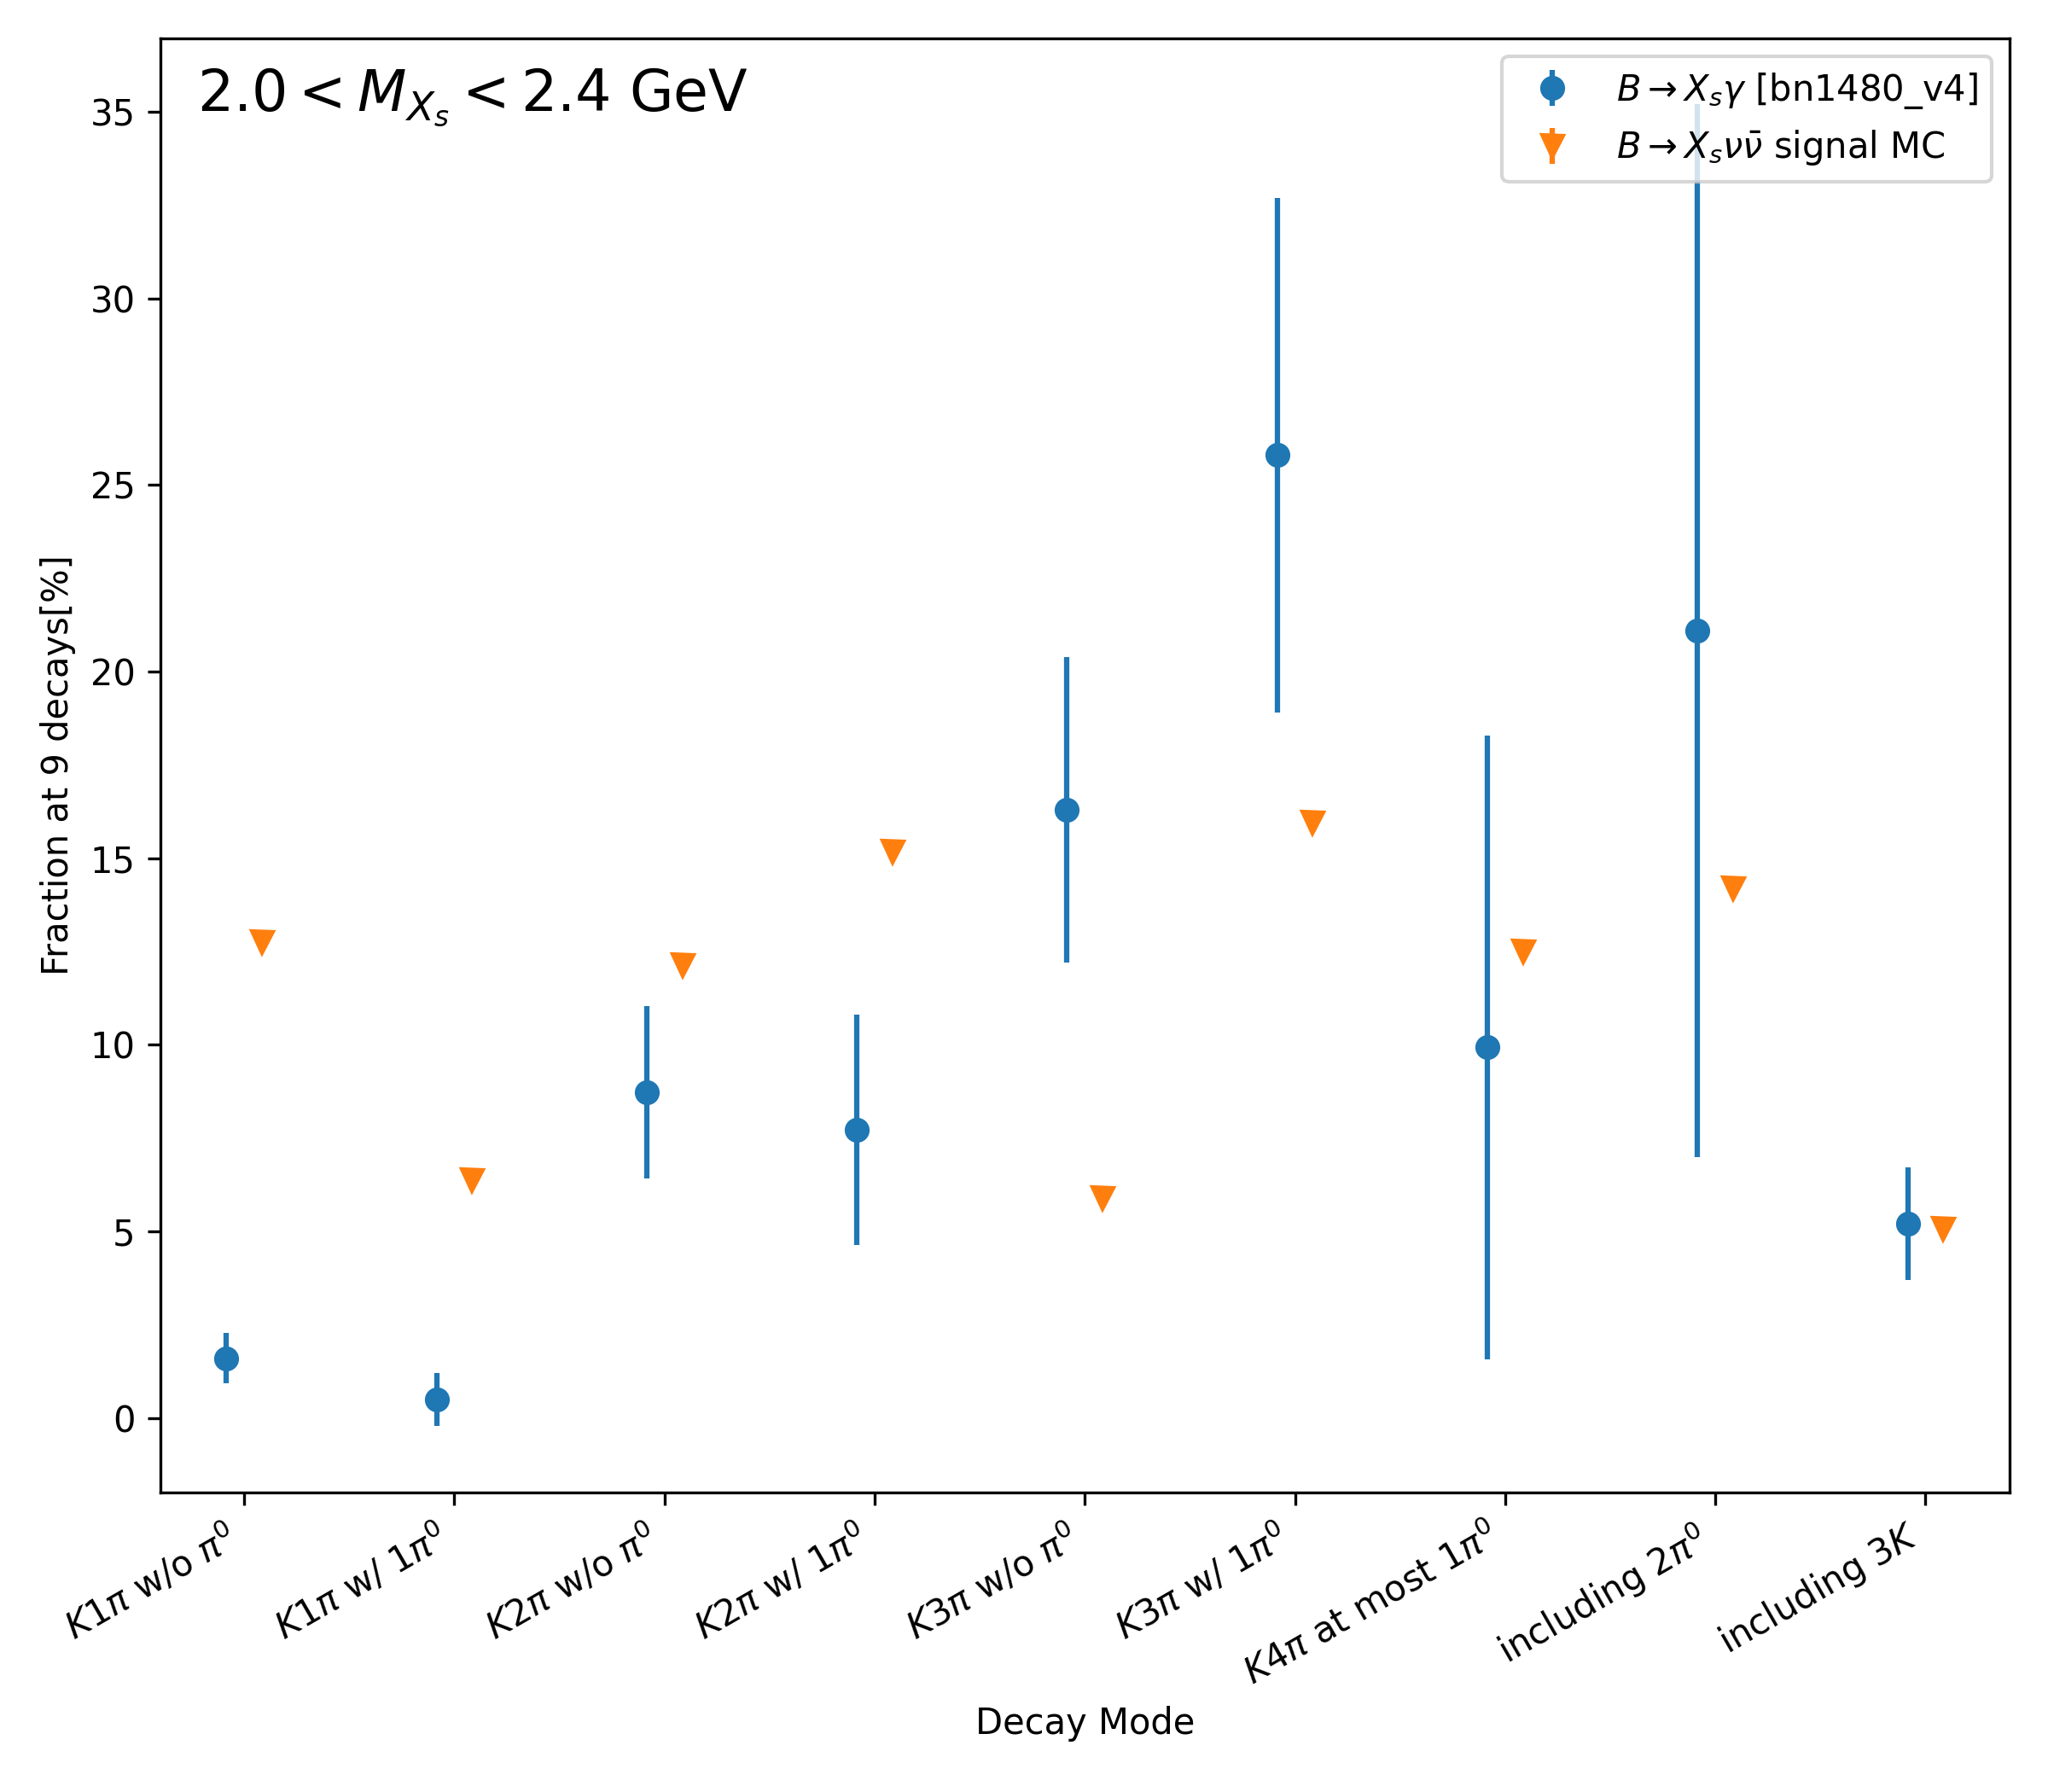
\includegraphics[width=0.32\textwidth]{./picture/systematic/fraction_2.0_2.4.png}}
  \caption{Fragmentation fractions of the nine decay-mode categories. The fractions are normalized within these nine categories and therefore sum to 100\%. The blue points show the results of the $B \rightarrow X_{s} \gamma$ study, and the orange points show the corresponding fractions in the $B \rightarrow X_{s} \nu \bar{\nu}$ signal MC sample.}
  \label{fig:fragmentation_Xs}
\end{figure}

\section{Mismodelling of $B\rightarrow X_{s}n\bar{n}$ decays}
\label{sec:Xsnnbar_correction}
In the official Belle II simulation, $B\rightarrow K^{(*)}n\bar{n}$ decays are generated according to a flat phase-space model.
However, experimental measurements of $B\rightarrow K^{(*)}p\bar{p}$ decays~\cite{Kplus_ppbar,Kstarplus_ppbar,Kzero_ppbar} show $M_{p\bar{p}}$ distributions that differ from a flat phase-space model.
Figures~\ref{fig:Knn_distribution}--\ref{fig:K0starnn_distribution} compare the measured distributions with those obtained from the official MC samples.
\begin{figure}
  \centering
  \subfloat{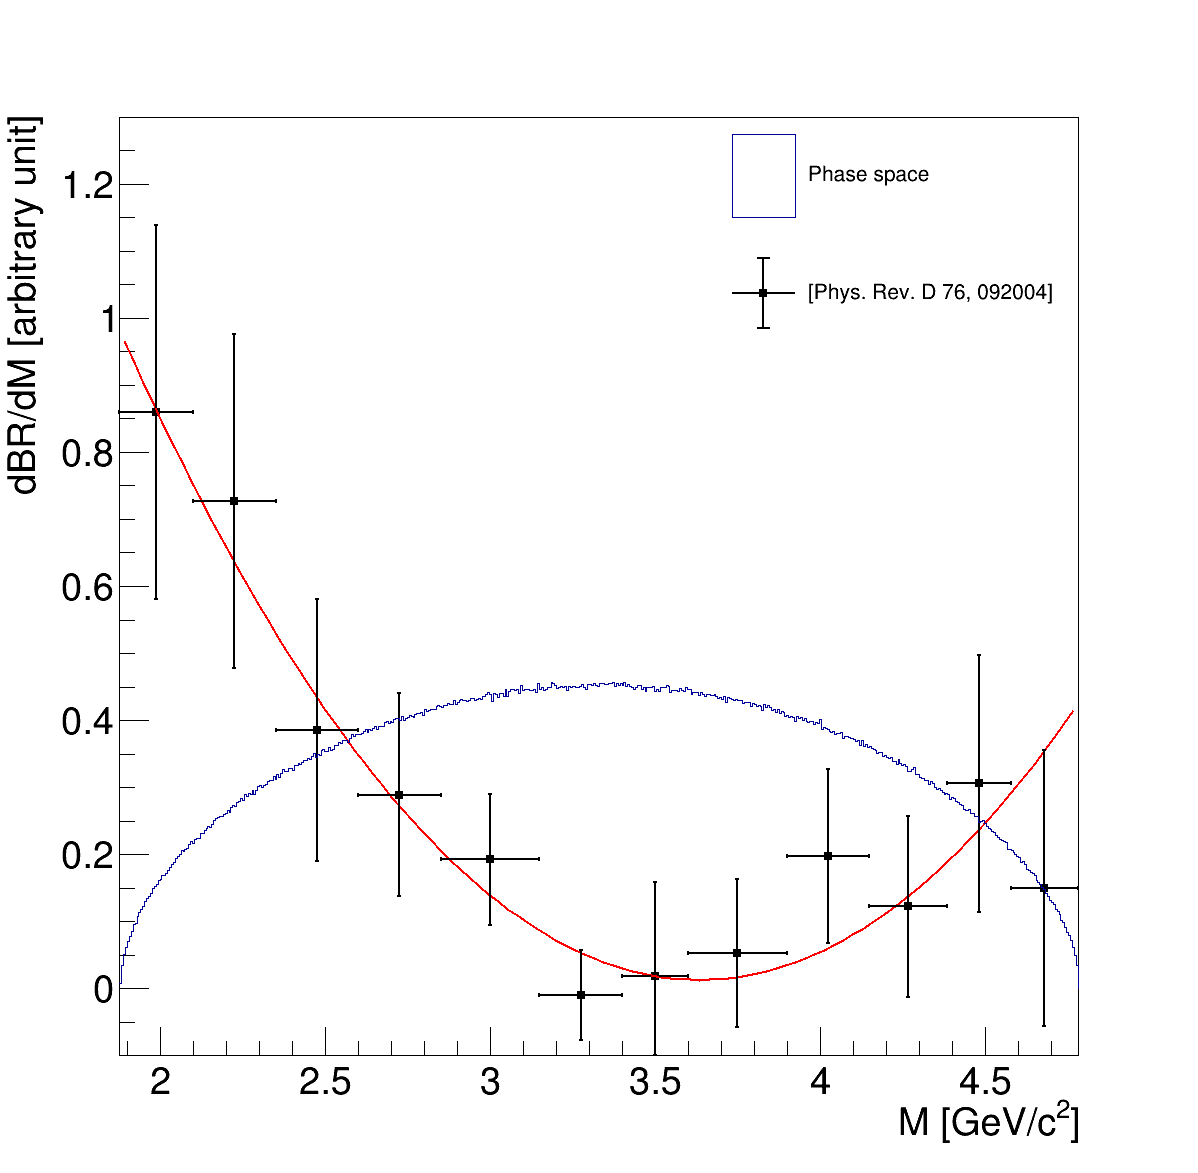
\includegraphics[width=0.4\textwidth]{./picture/systematic/invMdistribution_Knn_OLD.png}}
  \subfloat{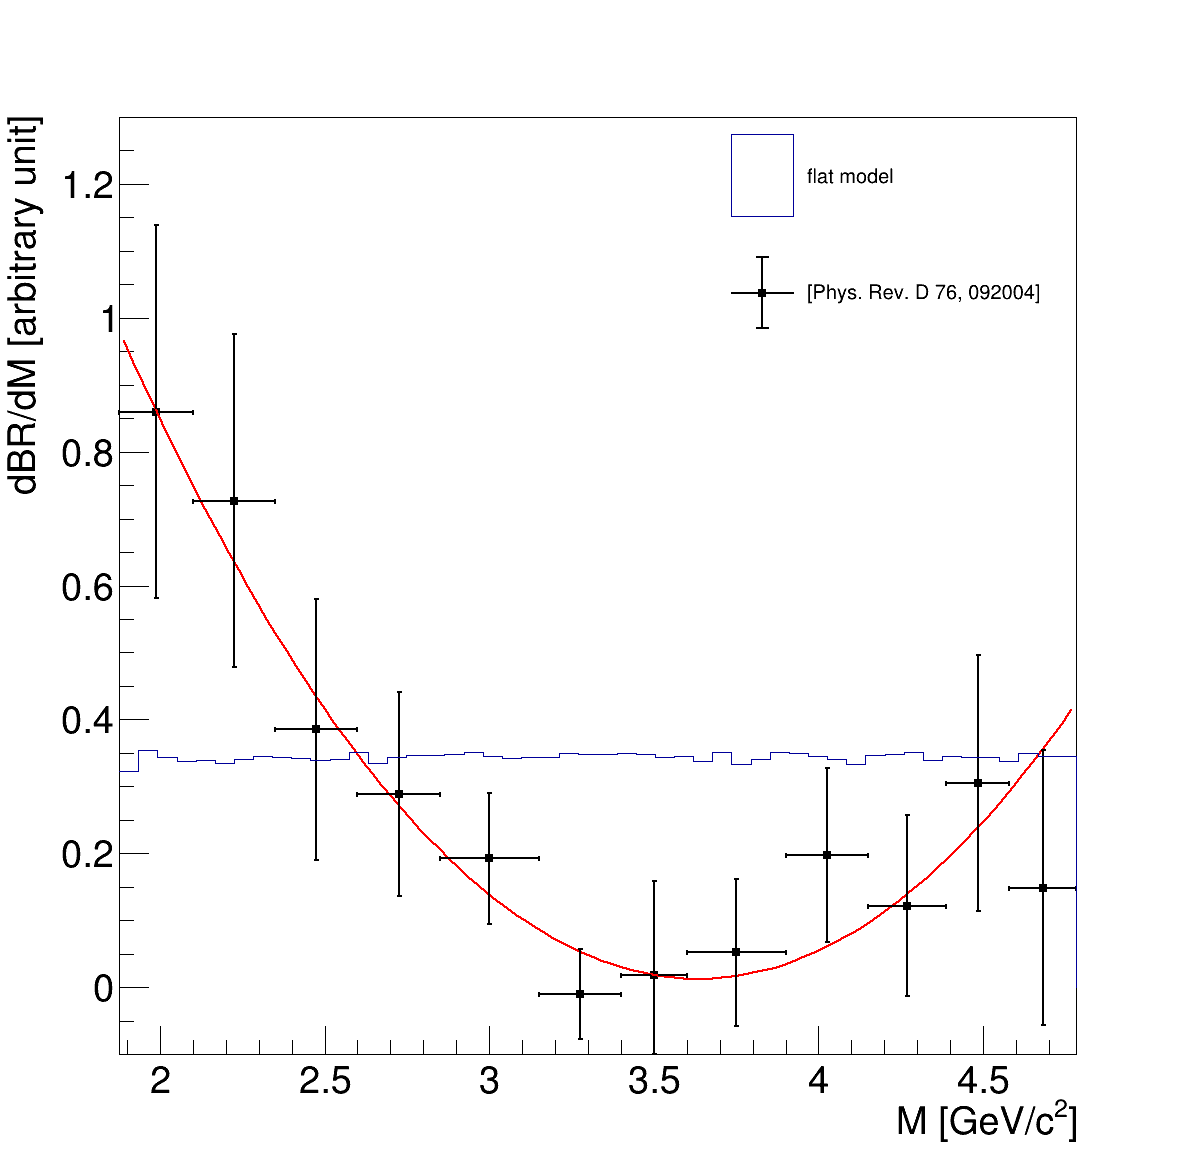
\includegraphics[width=0.4\textwidth]{./picture/systematic/invMdistribution_Knn.png}}
  \caption{Distribution of the invariant mass of the baryon--antibaryon pair. The black points show the distribution of $B^{0} \rightarrow K^{0}p\bar{p}$ decays. The blue histogram shows the distribution of $B^{+} \rightarrow K^{+}n\bar{n}$ decays generated using (left) a flat phase-space model and (right) a model with a flat $M_{n\bar{n}}$ distribution.}
  \label{fig:Knn_distribution}
\end{figure}
\begin{figure}
  \centering
  \subfloat{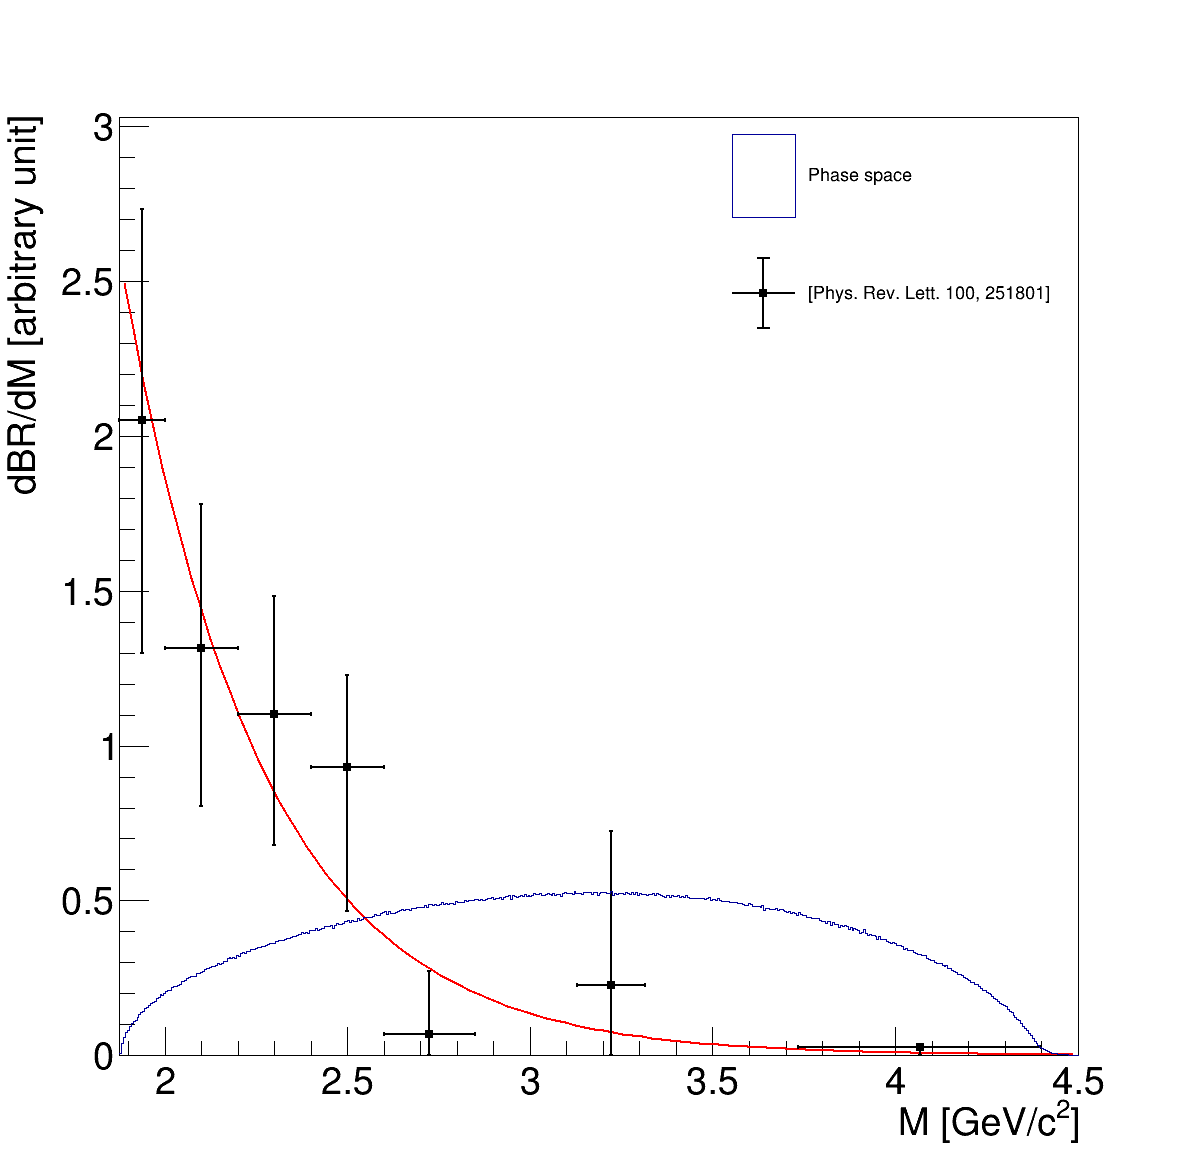
\includegraphics[width=0.4\textwidth]{./picture/systematic/invMdistribution_Kstarnn_OLD.png}}
  \subfloat{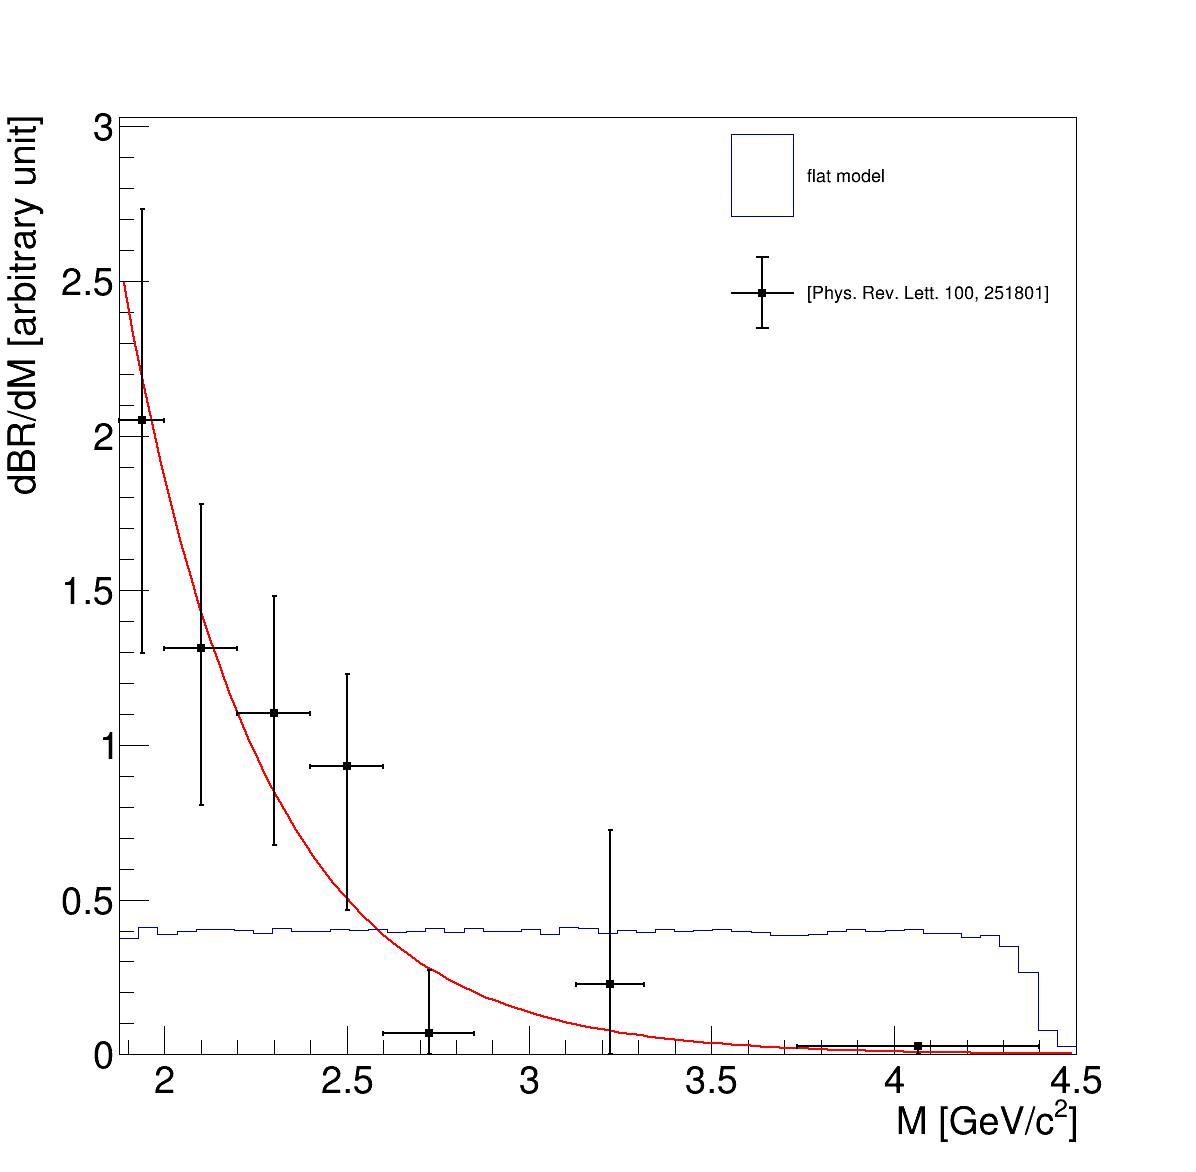
\includegraphics[width=0.4\textwidth]{./picture/systematic/invMdistribution_Kstarnn.png}}
  \caption{Distribution of the invariant mass of the baryon--antibaryon pair. The black points show the distribution of $B^{0} \rightarrow K^{*0}p\bar{p}$ decays. The blue histogram shows the distribution of $B^{+} \rightarrow K^{*+}n\bar{n}$ decays generated using (left) a flat phase-space model and (right) a model with a flat $M_{n\bar{n}}$ distribution.}
  \label{fig:Kstarnn_distribution}
\end{figure}
\begin{figure}
  \centering
  \subfloat{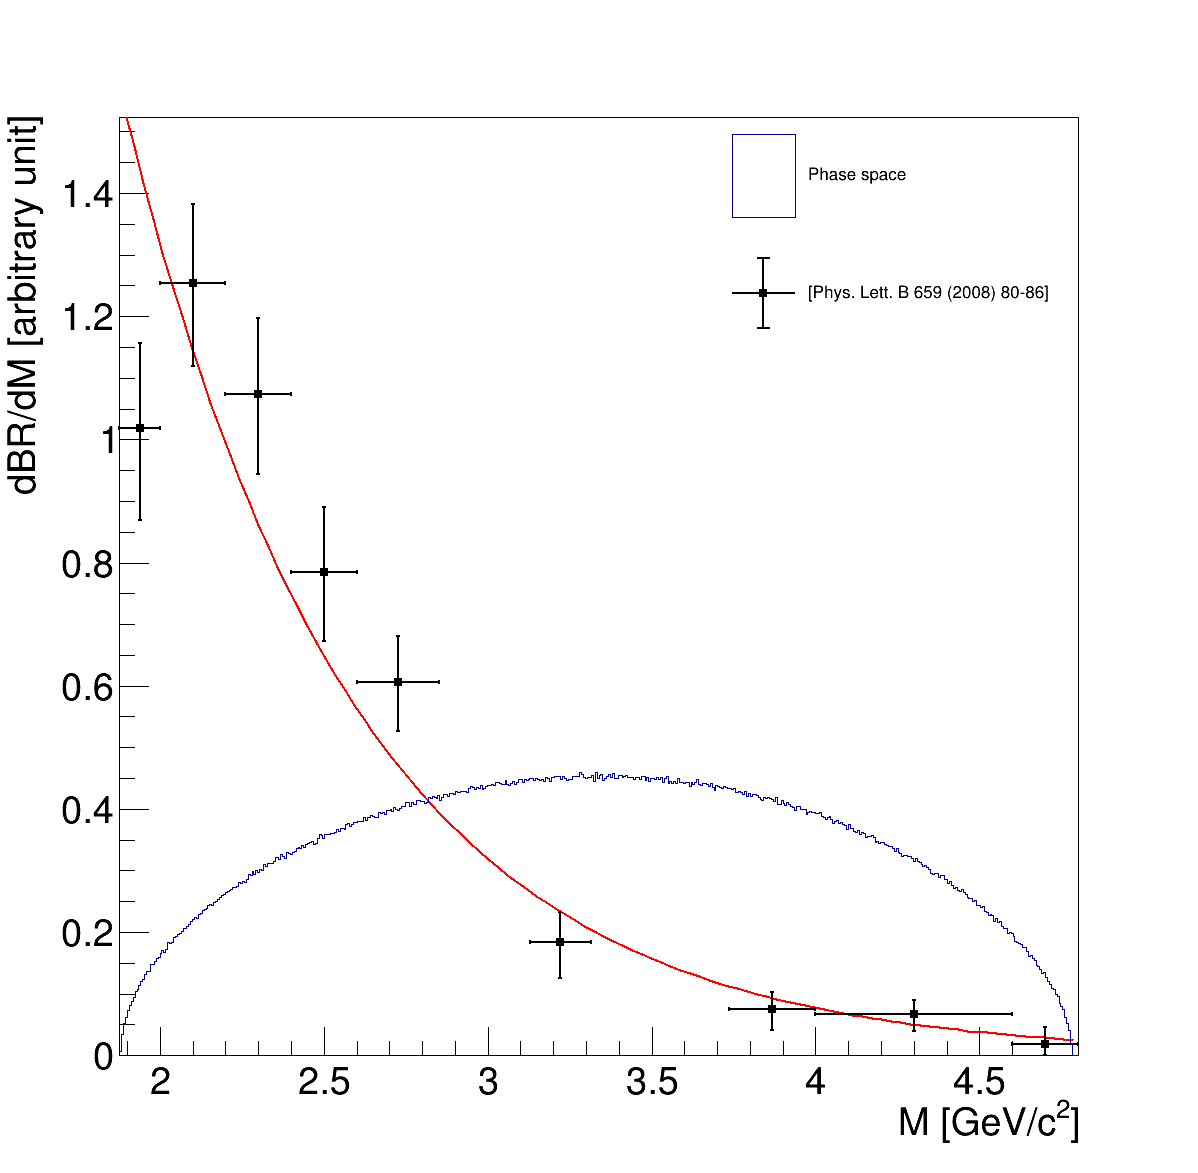
\includegraphics[width=0.4\textwidth]{./picture/systematic/invMdistribution_K0nn_OLD.png}}
  \subfloat{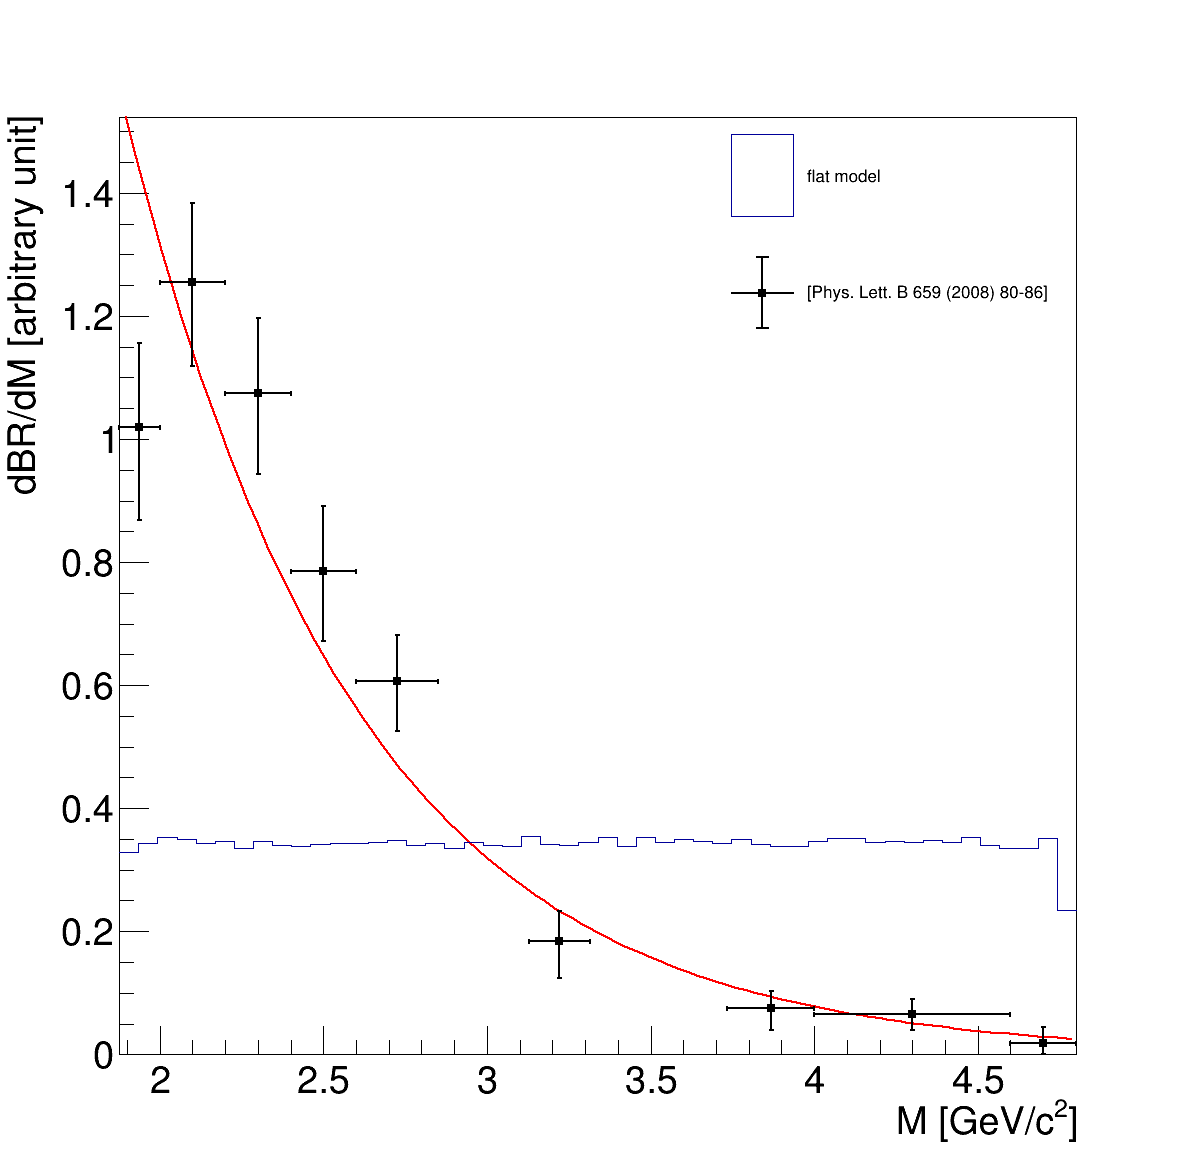
\includegraphics[width=0.4\textwidth]{./picture/systematic/invMdistribution_K0nn.png}}
  \caption{Distribution of the invariant mass of the baryon--antibaryon pair. The black points show the distribution of $B^{+} \rightarrow K^{+}p\bar{p}$ decays. The blue histogram shows the distribution of $B^{0} \rightarrow K^{0}n\bar{n}$ decays generated using (left) a flat phase-space model and (right) a model with a flat $M_{n\bar{n}}$ distribution.}
  \label{fig:K0nn_distribution}
\end{figure}
\begin{figure}
  \centering
  \subfloat{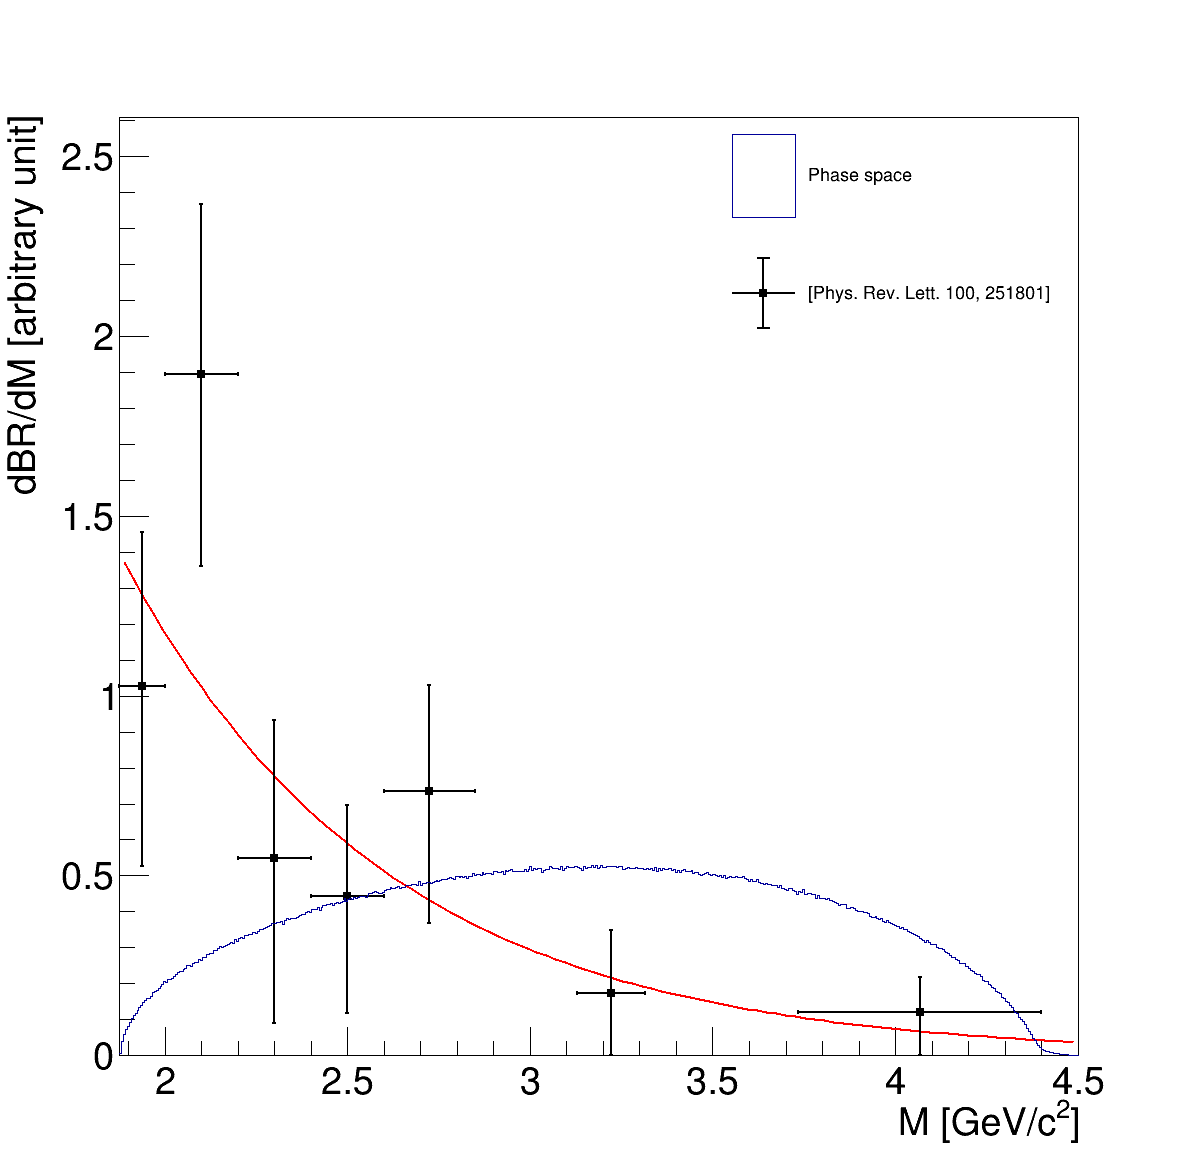
\includegraphics[width=0.4\textwidth]{./picture/systematic/invMdistribution_K0starnn_OLD.png}}
  \subfloat{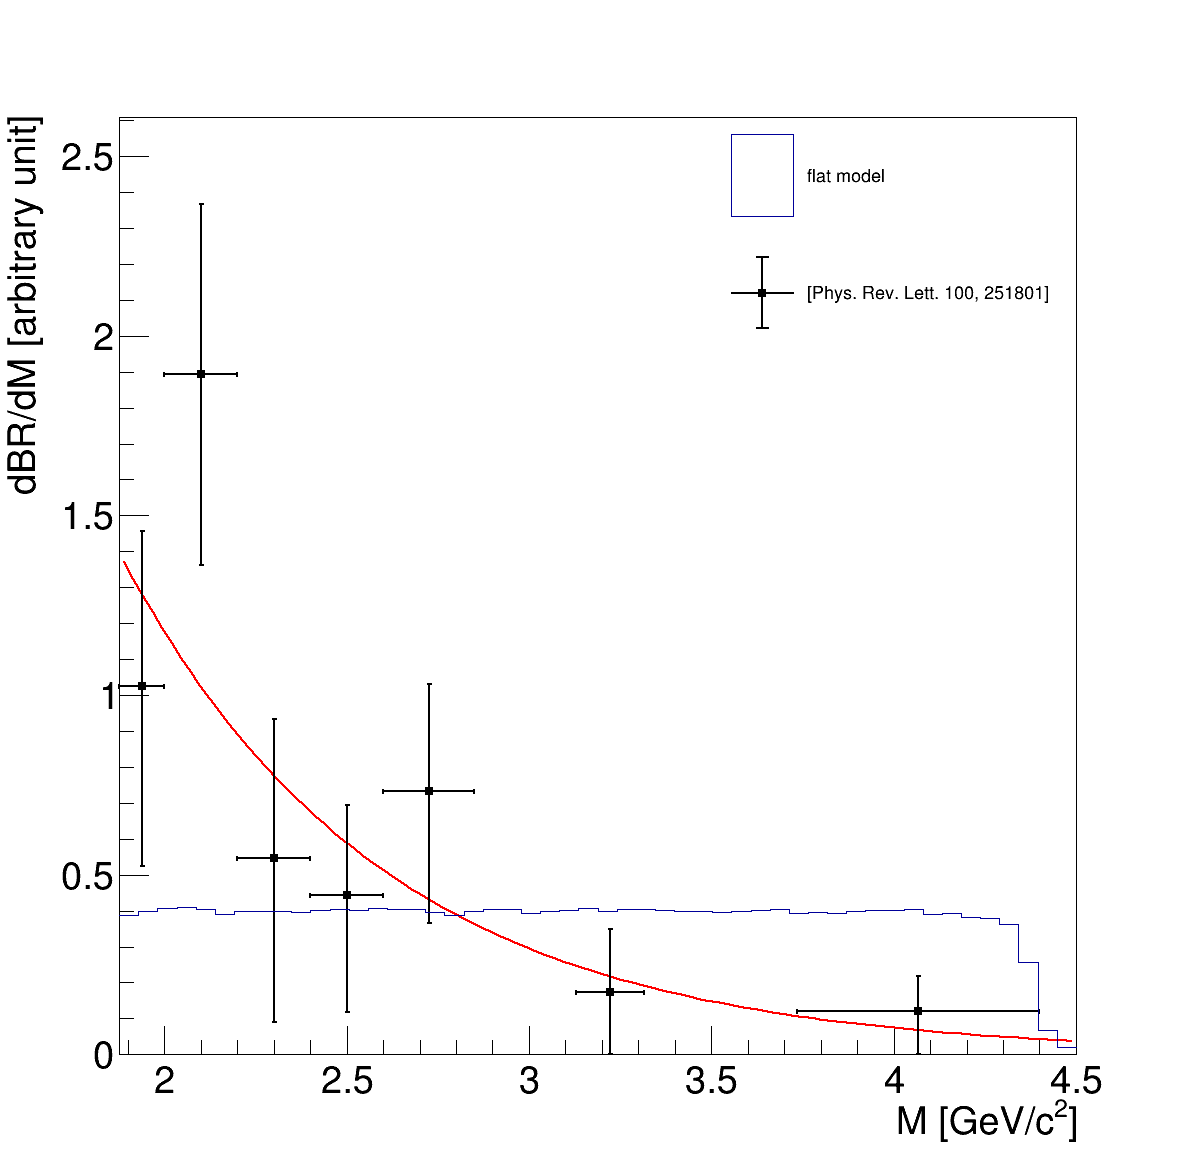
\includegraphics[width=0.4\textwidth]{./picture/systematic/invMdistribution_K0starnn.png}}
  \caption{Distribution of the invariant mass of the baryon--antibaryon pair. The black points show the distribution of $B^{0} \rightarrow K^{*0}p\bar{p}$ decays. The blue histogram shows the distribution of $B^{0} \rightarrow K^{*0}n\bar{n}$ decays generated using (left) a flat phase-space model and (right) a model with a flat $M_{n\bar{n}}$ distribution.}
  \label{fig:K0starnn_distribution}
\end{figure}

As discussed in Section~\ref{subsec:backgroundMC}, the official $B\rightarrow K^{(*)}n\bar{n}$ samples are replaced with private MC samples generated with a flat $M_{n\bar{n}}$ distribution.
Correction factors are then applied to these private samples to reproduce the observed $M_{p\bar{p}}$ distributions.
The measured $M_{p\bar{p}}$ distributions are fitted to obtain the correction functions.
An exponential function is used to fit the $B^{+}\rightarrow K^{+}p\bar{p}$, $B^{+}\rightarrow K^{*+}p\bar{p}$, and $B^{0}\rightarrow K^{*0}p\bar{p}$ distributions.
A second-order polynomial is used for the $B^{0}\rightarrow K^{0}p\bar{p}$ distribution.
The red curves in Figures~\ref{fig:Knn_distribution}--\ref{fig:K0starnn_distribution} show the fitted functions.
The correction factors are defined as the ratios of the fitted functions to the distributions generated with a flat $M_{n\bar{n}}$ model.

A correction is also required for the remaining $B\rightarrow X_{s}n\bar{n}$ decays.
However, no previous experimental measurement of $B\rightarrow X_{s}p\bar{p}$ decays is available.
Therefore, a study of $B\rightarrow X_{s}p\bar{p}$ decays is performed.
To reconstruct $B\rightarrow X_{s}p\bar{p}$ decays, the $X_{s}$ and $B_{\textrm{tag}}$ candidates are reconstructed using the method described in Section~\ref{sec:rec_and_selec}.
Additionally, proton candidates are selected by the following criteria:
\begin{itemize}
  \item $\texttt{protonID} > 0.6$
  \item $dr < 0.5~\textrm{cm}$ and $\left| dz \right| < 2~\textrm{cm}$
  \item $\texttt{nCDCHits} > 20$
  \item $\texttt{nPXDHits} > 0$
\end{itemize}
The selected proton and antiproton candidates are combined with the $X_{s}$ candidate to reconstruct $B_{\textrm{sig}}\rightarrow X_{s}p\bar{p}$.
Several selection requirements are applied after reconstruction.
Table~\ref{tab:cutflow_ppbar} shows the cut flow for the $B\rightarrow X_{s}p\bar{p}$ analysis.
To suppress background, the Fox--Wolfram ratio $R_{2}$, the cosine of the angle between the thrust axis of $B_{\textrm{sig}}$ and that of its ROE, and the event sphericity are used~\cite{Fox:1978vw}.
Figure~\ref{fig:Mbc_ppbar} shows the $M_{\textrm{bc}}$ distribution of $B_{\textrm{sig}}$ candidates after the BCS.
\begin{table}
\caption{Cut flow for the $B\rightarrow X_{s}p\bar{p}$ analysis.}
  \renewcommand{\arraystretch}{1.2}
  \centering
\begin{tabular}{ p{7cm} }
 \hline
  \hline
Selection \\
 \hline
Generated \\
Skim \\
Reconstruction and preselections \\
$M_{\textrm{bc}}>5.2~\textrm{GeV}/c^{2}$ for $B_{\textrm{sig}}$ \\
$\left|\Delta E\right|<0.05~\textrm{GeV}$ for $B_{\textrm{sig}}$\\
$\left|\Delta E\right|<0.2~\textrm{GeV}$ for $B_{\textrm{tag}}$\\
$E_{\textrm{ecl}} < 1.3~\textrm{GeV}$\\
$\texttt{sphericity} > 0.2$\\
$\texttt{R2} < 0.4$ for $B_{\textrm{sig}}$\\
$\texttt{cosTBTO} < 0.9$ for $B_{\textrm{sig}}$\\
$M_{X_{s}} > 1.0~\textrm{GeV}/c^{2}$\\
BCS \\
  \hline
   \hline
\end{tabular}
    \label{tab:cutflow_ppbar}
\end{table}
\begin{figure}[h]
  \centering
  \subfloat{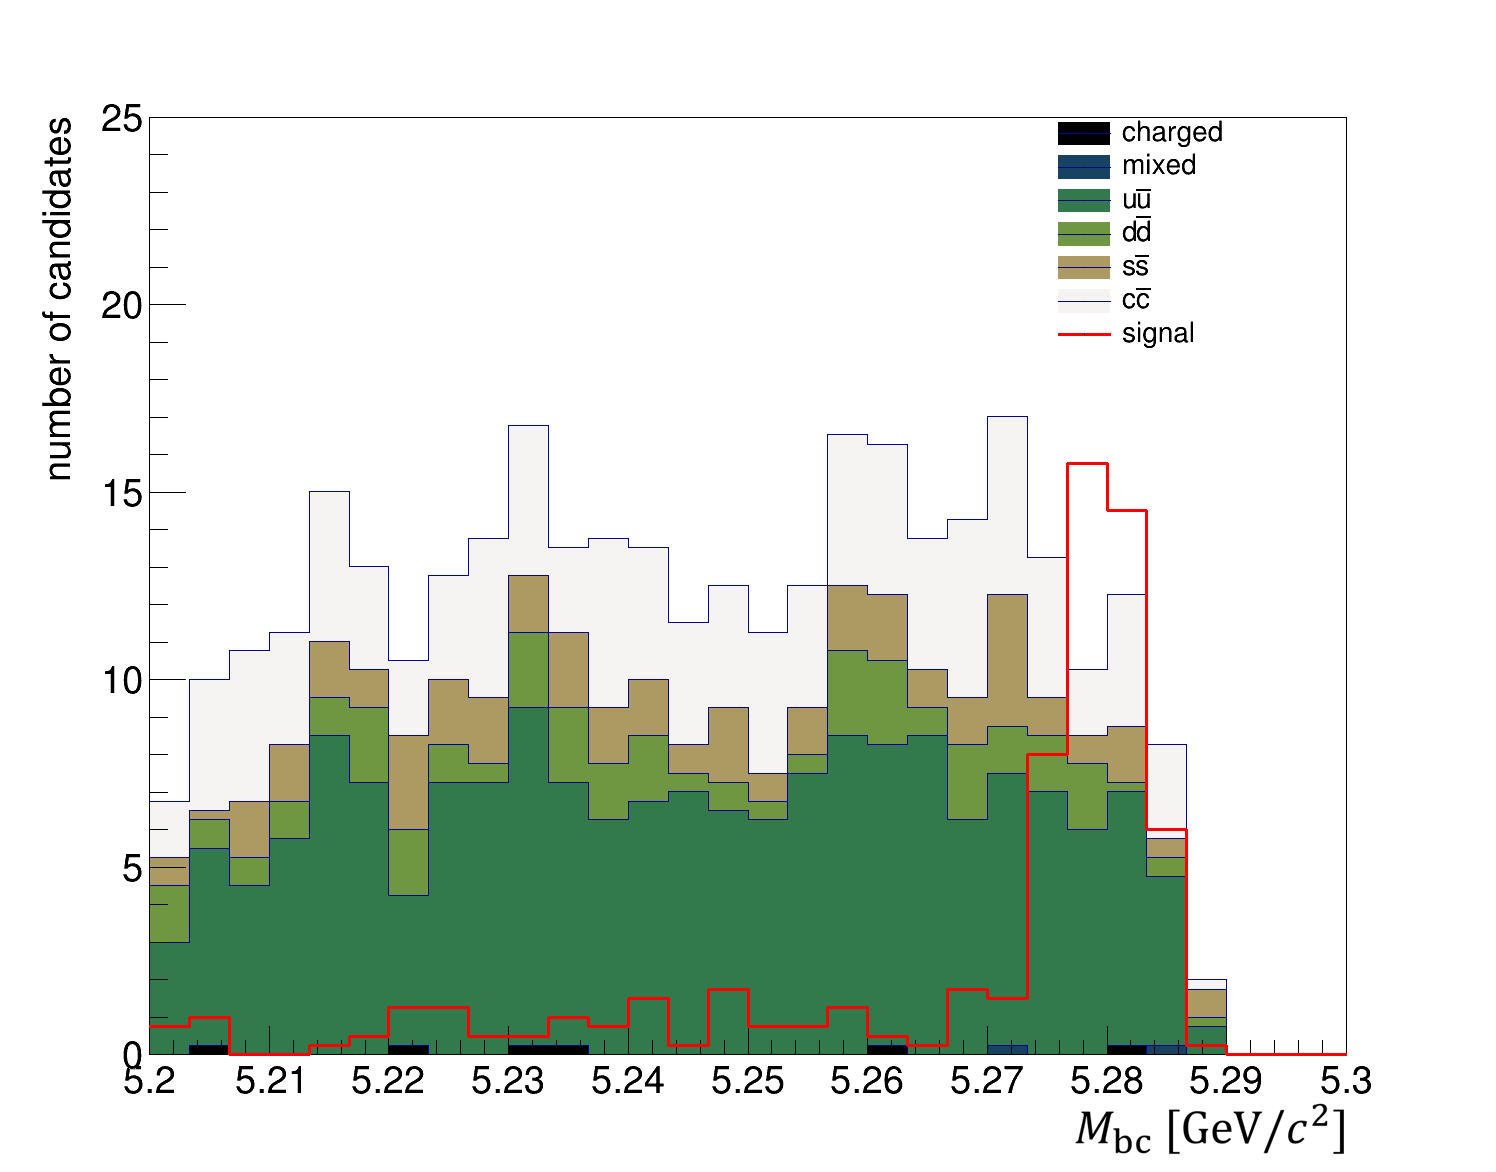
\includegraphics[width=0.6\textwidth]{./picture/Xspp/Plot_Mbc.png}}
  \caption{Distribution of $M_{\textrm{bc}}$ for the $B_{\textrm{sig}}$ candidates in the $B \rightarrow X_{s}p\bar{p}$ analysis.}
  \label{fig:Mbc_ppbar}
\end{figure}

To determine the $M_{p\bar{p}}$ distribution, fits are performed in several $M_{p\bar{p}}$ regions.
Table~\ref{tab:function_ppbar} summarizes the fit model used in the $B\rightarrow X_{s}p\bar{p}$ analysis.
Figure~\ref{fig:ppbar_fit_result} shows the fit results in the different $M_{p\bar{p}}$ regions.
\begin{table}[]
\caption{Fit model used in the $B\rightarrow X_{s}p\bar{p}$ analysis.}
 \centering
  \begin{tabular}{p{3cm} p{3cm} p{6cm}}
    \hline
    \hline
    Function                    & Parameter &                      \\
    \hline
  \multirow{4}{*}{Crystal Ball} & mean      & fixed using $B\rightarrow K^{(*)}p\bar{p}$ data \\
                                & width     & fixed using $B\rightarrow K^{(*)}p\bar{p}$ data \\
                                & alpha     & fixed from MC \\
                                & n         & fixed from MC \\
                                \hline
  \multirow{3}{*}{ARGUS}        & endpoint  & fixed to the beam energy \\
                                & curvature & floated \\
                                & power     & fixed to 0.5 \\
  \hline
  \hline
  \end{tabular}
  \label{tab:function_ppbar}
\end{table}
\begin{figure}[h]
    \centering
    \subfloat[][$1.800 < M_{p\bar{p}} < 2.425$]
    {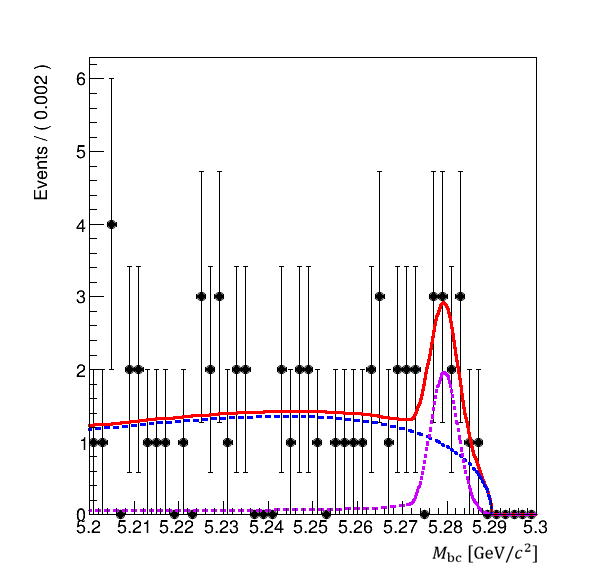
\includegraphics[width=0.32\textwidth]{./picture/Xspp/ppbar_MXs1.png}}
    \subfloat[][$2.425 < M_{p\bar{p}} < 3.050$]
    {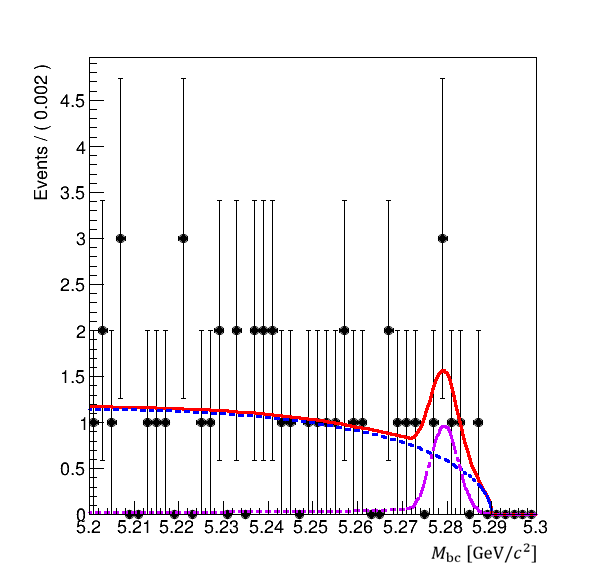
\includegraphics[width=0.32\textwidth]{./picture/Xspp/ppbar_MXs2.png}}
    \subfloat[][$3.050 < M_{p\bar{p}} < 3.675$]
    {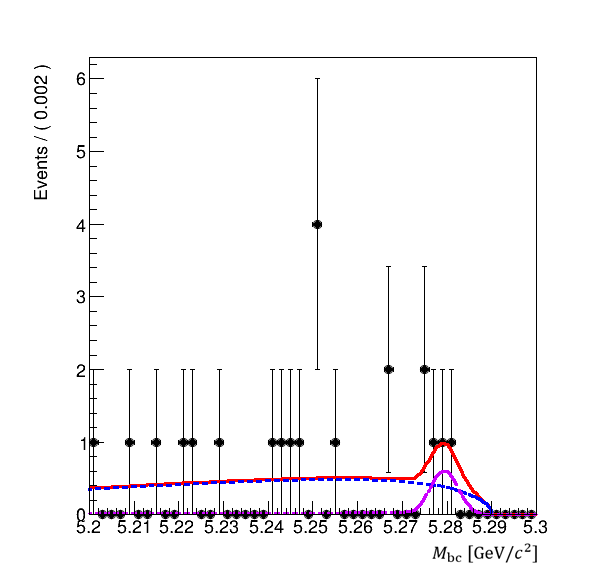
\includegraphics[width=0.32\textwidth]{./picture/Xspp/ppbar_MXs3.png}}

    \caption{
    Fit results for the $B\rightarrow X_{s}p\bar{p}$ analysis in three
    $M_{p\bar{p}}$ intervals, where $M_{p\bar{p}}$ is expressed in
    $\textrm{GeV}/c^{2}$.
    The fit variable is $M_{\textrm{bc}}$ of the
    $B_{\textrm{sig}}$ candidate.
    The blue curve shows the background component, the purple curve shows
    the $B\rightarrow X_{s}p\bar{p}$ signal component, and the red curve
    shows their sum.
    }
    \label{fig:ppbar_fit_result}
\end{figure}

Figure~\ref{fig:ppbar_data_MC} compares the $M_{p\bar{p}}$ distributions in data and MC.
The blue points show the event yields in data, and the red points show the corresponding MC yields.
For $M_{p\bar{p}}>3.675~\textrm{GeV}/c^{2}$, no events are observed in the region $M_{\textrm{bc}}>5.27~\textrm{GeV}/c^{2}$, and only one event is observed in the sideband $5.2<M_{\textrm{bc}}<5.27~\textrm{GeV}/c^{2}$, where $M_{\textrm{bc}}$ is calculated for the $B_{\textrm{sig}}$ candidate.
Therefore, the yield is assumed to be zero in the region $M_{p\bar{p}}>3.675~\textrm{GeV}/c^{2}$.
The correction factors are defined as the ratios of the data yields to the MC yields.
\begin{figure}[h]
  \centering
  \subfloat{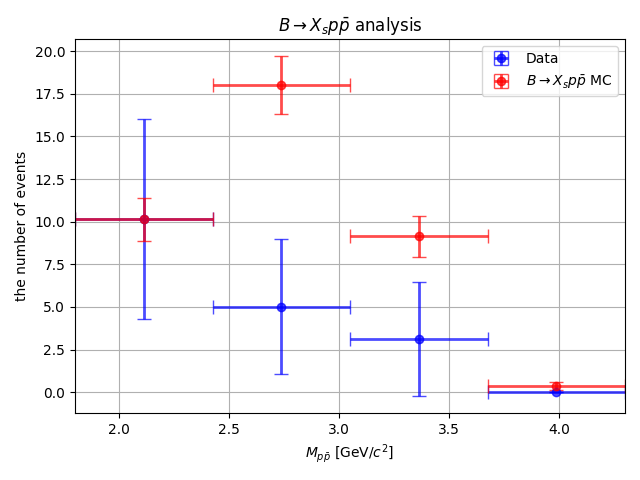
\includegraphics[width=0.6\textwidth]{./picture/Xspp/Xsnn.png}}
  \caption{Comparison of the $M_{p\bar{p}}$ distributions in data and MC for $B\rightarrow X_{s}p\bar{p}$ decays. The blue points show the signal yields extracted from data, and the red points show the expected yields from MC.}
  \label{fig:ppbar_data_MC}
\end{figure}

\section{Mismodelling of $B\rightarrow X_{s}K_{L}^{0}K_{L}^{0}$ decays}
\label{sec:XsKLKL_correct}
In the $B^{+}\rightarrow K^{+}\nu\bar{\nu}$ analysis~\cite{Belle-II:2023esi}, $B^{+}\rightarrow K^{+}K_{L}^{0}K_{L}^{0}$ decays were found to be one of the major sources of systematic uncertainty.
Therefore, corrections are applied to $B\rightarrow X_{s}K_{L}^{0}K_{L}^{0}$ decays.

To correct the $B^{+}\rightarrow K^{+}K_{L}^{0}K_{L}^{0}$ decay model, experimental results for $B^{+}\rightarrow K^{+}K_{S}^{0}K_{S}^{0}$ decays are used.
According to Ref.~\cite{BaBar:2012iuj}, the dynamical amplitude for the $B^{+}\rightarrow K^{+}K_{S}^{0}K_{S}^{0}$ decay can be modeled as follows:
\begin{equation}
    F^{L}_{j}\left(s_{12}, s_{23} \right) = R_{j}\left(m \right) X_{L}\left( \left|\overrightarrow{p}^{*} \right| r' \right) X_{L}\left( \left|\overrightarrow{q} \right| r \right) T_{j} \left(L,\overrightarrow{p},\overrightarrow{q} \right),
\end{equation}
where $s_{12}$ is the squared invariant mass of the $K_{S}^{0}K_{S}^{0}$ system, and $s_{23}$ is the larger of the two squared invariant masses of the $K_{S}^{0}K^{+}$ combinations.

In the official Belle II simulation, the $B^{+}\rightarrow K^{+}K_{L}^{0}K_{L}^{0}$ sample contains both resonant and nonresonant components.
The nonresonant component is generated using a flat phase-space model.
In this analysis, the resonant $B^{+}\rightarrow K^{+}K_{L}^{0}K_{L}^{0}$ components are removed.
More specifically, $B^{+}\rightarrow K^{+} K_{L}^{0} K_{L}^{0}$ decays from $B^{+}\rightarrow K^{+} f_{0}(980)$, $B^{+}\rightarrow K^{+} f_{0}(1370)$, $B^{+}\rightarrow K^{+} f_{2}(1270)$, $B^{+}\rightarrow K^{+} f'_{2}(1525)$, and $B^{+}\rightarrow K^{+} \chi_{c0}(1P)$ decays are removed.
These are all resonant decay modes that contribute to $B^{+}\rightarrow K^{+}K_{L}^{0}K_{L}^{0}$ in the official simulation.
A correction factor is then applied to the nonresonant $B^{+}\rightarrow K^{+}K_{L}^{0}K_{L}^{0}$ component.
Figure~\ref{fig:KKL0KL0_kinematics} shows the Dalitz plots for $B^{+}\rightarrow K^{+}K_{L}^{0}K_{L}^{0}$ decays generated using a flat phase-space model and a model based on the experimental results of Ref.~\cite{BaBar:2012iuj}.
A small distortion is present in the flat-phase-space distribution because of \texttt{PHOTOS}.
Because this effect is small, additional correction for \texttt{PHOTOS} is not considered.
The correction factor is obtained from the bin-by-bin ratio of the two Dalitz-plot distributions shown in Figure~\ref{fig:KKL0KL0_kinematics}.
\begin{figure}
  \centering
  \subfloat[]{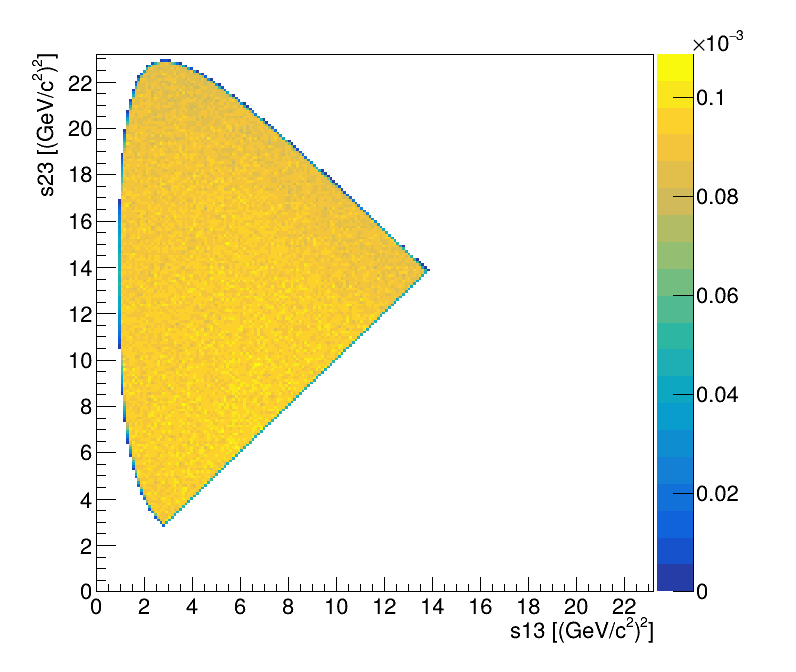
\includegraphics[width=0.45\textwidth]{./picture/systematic/PHSP_KKLKL.png}}
  \subfloat[]{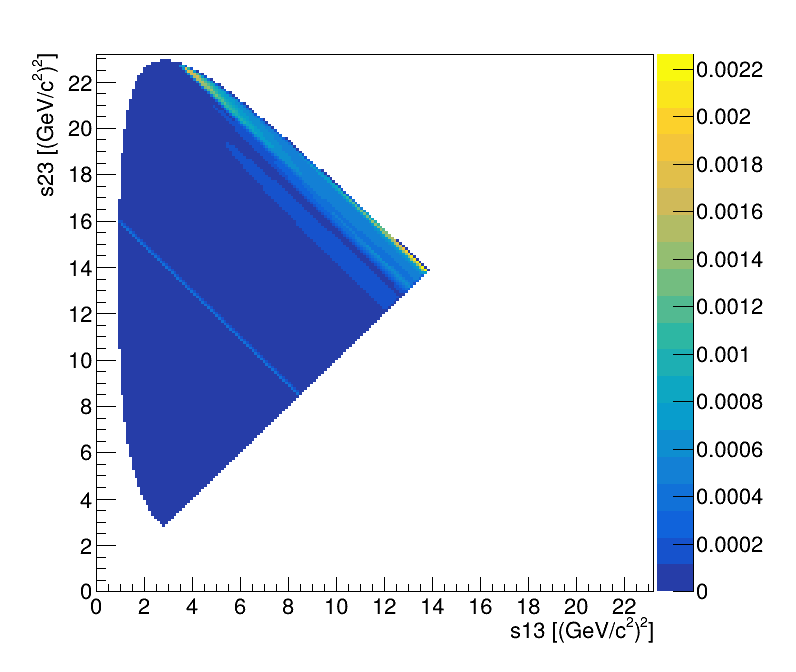
\includegraphics[width=0.45\textwidth]{./picture/systematic/model_KKLKL.png}}
  \caption{Dalitz plots for $B^{+}\rightarrow K^{+}K_{L}^{0}K_{L}^{0}$ decays generated using (a) a flat phase-space model and (b) a model based on experimental results~\cite{BaBar:2012iuj}. Here, $s_{12}$ is the squared invariant mass of the $K_{L}^{0}K_{L}^{0}$ system, and $s_{23}$ is the larger of the two squared invariant masses of the $K_{L}^{0}K^{+}$ combinations. A small distortion is present in the flat-phase-space distribution because of \texttt{PHOTOS}.}
  \label{fig:KKL0KL0_kinematics}
\end{figure}
A correction factor for the branching ratio is also applied.
It is calculated using the PDG value as follows~\cite{ParticleDataGroup:2024cfk}:
\begin{equation}
    w =
    \frac{
    BR_{\textrm{PDG}}(B^{+}\rightarrow K^{+}K_{S}^{0}K_{S}^{0})
    }{
    BR_{\textrm{MC}}^{\textrm{nonres}}
    (B^{+}\rightarrow K^{+}K_{L}^{0}K_{L}^{0})
    }.
\end{equation}

The correction factor for $B^{0}\rightarrow K_{S}^{0}K_{L}^{0}K_{L}^{0}$ is obtained using a similar method.
However, a different procedure is required.
The $B^{0} \rightarrow K_{S}^{0} K_{L}^{0} K_{L}^{0}$ decay contains a resonant contribution from $\phi\rightarrow K_{S}^{0}K_{L}^{0}$.
In contrast, the $B^{0}\rightarrow K_{S}^{0}K_{S}^{0}K_{S}^{0}$ decay contains no contribution from $\phi\rightarrow K_{S}^{0}K_{L}^{0}$.
Consequently, the Dalitz-plot distribution for $B^{0}\rightarrow K_{S}^{0}K_{S}^{0}K_{S}^{0}$ is not identical to that for $B^{0}\rightarrow K_{S}^{0}K_{L}^{0}K_{L}^{0}$.

According to the calculation~\cite{Gronau:2005ax}, the relation between $B^{0}\rightarrow K_{S}^{0} K_{S}^{0} K_{S}^{0}$ and $B^{0} \rightarrow K_{S}^{0} K_{L}^{0} K_{L}^{0}$ is
\begin{equation}
    BR(B^{0}\rightarrow K_{S}^{0} K_{S}^{0} K_{S}^{0}) = 3 \times BR(B^{0}\rightarrow K_{S}^{0} K_{L}^{0} K_{L}^{0}),
\end{equation}
where the $\phi K$ contribution is excluded.
Therefore, all resonant contributions are removed except for $B^{0}\rightarrow\phi K_{L}^{0}$.
More specifically, $B^{0}\rightarrow K_{S}^{0} K_{L}^{0} K_{L}^{0}$ decays from $B^{0}\rightarrow K^{0} f_{0}(980)$, $B^{0}\rightarrow K^{0} f_{0}(1370)$, $B^{0}\rightarrow K^{0} f_{2}(1270)$, $B^{0}\rightarrow K^{0} f'_{2}(1525)$, and $B^{0}\rightarrow K^{0} \chi_{c0}(1P)$ decays are removed.
These modes comprise all resonant contributions to $B^{0}\rightarrow K_{S}^{0}K_{L}^{0}K_{L}^{0}$ included in the official simulation, except $B^{0} \rightarrow \phi K_{L}^{0}$.
For the $B^{0}\rightarrow\phi K_{L}^{0}$ component, the branching ratio in the official Belle II simulation is corrected using the PDG value~\cite{ParticleDataGroup:2024cfk}:
\begin{equation}
    w =
    \frac{
    BR_{\textrm{PDG}}(B^{0}\rightarrow \phi K_{L}^{0})
    }{
    BR_{\textrm{MC}}
    (B^{0}\rightarrow \phi K_{L}^{0})
    }.
\end{equation}
For the nonresonant $B^{0}\rightarrow K_{S}^{0}K_{L}^{0}K_{L}^{0}$ sample, the Dalitz-plot distribution measured in $B^{0}\rightarrow K_{S}^{0}K_{S}^{0}K_{S}^{0}$ decays is used to model the kinematics.
The $B^{0}\rightarrow K_{S}^{0} K_{S}^{0} K_{S}^{0}$ decay is modeled by the following formula~\cite{BaBar:2011ktx}:
\begin{equation}
    F^{L}_{j}\left(s_{\textrm{min}}, s_{\textrm{max}},L \right) = R_{j}\left(m \right) X_{L}\left( \left|\overrightarrow{p}^{*} \right| r' \right) X_{L}\left( \left|\overrightarrow{q} \right| r \right) T_{j} \left(L,\overrightarrow{p},\overrightarrow{q} \right),
\end{equation}
where $s_{\textrm{min}}$ and $s_{\textrm{max}}$ are the smallest and largest squared invariant masses of $K^{0}_{S}K^{0}_{S}$, respectively.
The correction factor is obtained from the bin-by-bin ratio of the Dalitz-plot distributions generated using a flat phase-space model and a model based on experimental results~\cite{BaBar:2011ktx}.
Figure~\ref{fig:KS0KL0KL0_kinematics} shows these Dalitz plots.
The branching ratio correction factor is calculated using the PDG value~\cite{ParticleDataGroup:2024cfk}:
\begin{equation}
    w =
    \frac{1}{3}
    \frac{
    BR_{\textrm{PDG}}
    (B^{0}\rightarrow K_{S}^{0}K_{S}^{0}K_{S}^{0})
    }{
    BR_{\textrm{MC}}^{\textrm{nonres}}
    (B^{0}\rightarrow K_{S}^{0}K_{L}^{0}K_{L}^{0})
    }.
\end{equation}
\begin{figure}
  \centering
  \subfloat[]{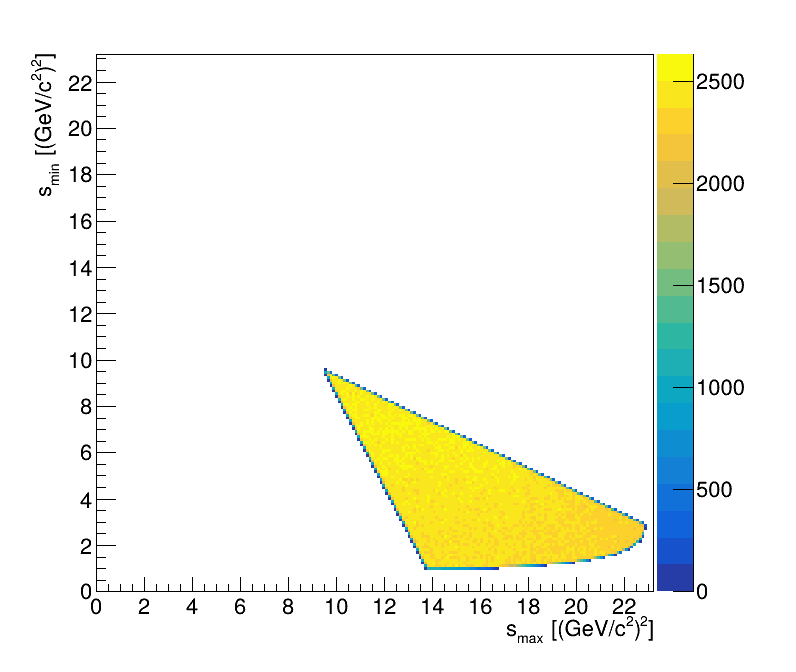
\includegraphics[width=0.45\textwidth]{./picture/systematic/PHSP_K0KLKL.png}}
  \subfloat[]{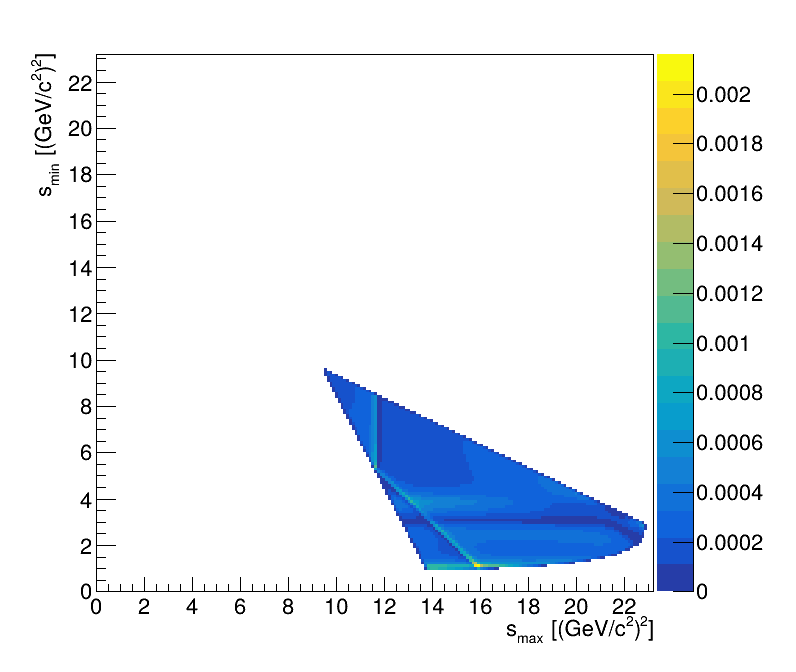
\includegraphics[width=0.45\textwidth]{./picture/systematic/model_K0KLKL.png}}
  \caption{Dalitz plots for $B^{0}\rightarrow K_{S}^{0}K_{L}^{0}K_{L}^{0}$ decays generated using (a) a flat phase-space model and (b) a model based on experimental results~\cite{BaBar:2011ktx}. Here, $s_{\textrm{min}}$ and $s_{\textrm{max}}$ are the smallest and largest squared invariant masses among the $K_{L}^{0}K_{L}^{0}$ and the two $K_{S}^{0}K_{L}^{0}$ combinations, respectively. A small distortion is present in the flat-phase-space distribution because of \texttt{PHOTOS}.}
  \label{fig:KS0KL0KL0_kinematics}
\end{figure}

To correct $B \rightarrow K^{*} K_{L}^{0} K_{L}^{0}$ and $B \rightarrow X_{s} K_{L}^{0} K_{L}^{0}$, experimental results for $B \rightarrow K^{*} K_{S}^{0} K_{S}^{0}$ and $B \rightarrow X_{s} K_{S}^{0} K_{S}^{0}$ decays are needed.
However, no such experimental measurements are available.
Therefore, studies of $B\rightarrow K^{*}K_{S}^{0}K_{S}^{0}$ and $B\rightarrow X_{s}K_{S}^{0}K_{S}^{0}$ decays are performed.

To reconstruct $B \rightarrow K^{*} K_{S}^{0} K_{S}^{0}$ decay, the $K\pi$ and $B_{\textrm{tag}}$ candidates are reconstructed using the method described in Section~\ref{sec:rec_and_selec}.
The $K\pi$ candidate is combined with two $K_{S}^{0}$ candidates to reconstruct $B_{\textrm{sig}}\rightarrow K^{*}K_{S}^{0}K_{S}^{0}$.
After the reconstruction, several cuts are applied. Table~\ref{tab:cutflow_KstarKLKL} shows the cut flow for $B \rightarrow K^{*} K_{S}^{0} K_{S}^{0}$ analysis.
Figure~\ref{fig:Mbc_KstarKLKL} shows the $M_{\textrm{bc}}$ distribution of the $B_{\textrm{sig}}$ candidates after BCS.
\begin{table}
\caption{Cut flow for the $B\rightarrow K^{*}K_{S}^{0}K_{S}^{0}$ analysis.}
  \renewcommand{\arraystretch}{1.2}
  \centering
\begin{tabular}{ p{7cm} }
 \hline
  \hline
Selection \\
 \hline
Generated \\
Skim \\
Reconstruction and preselections \\
$M_{bc}>5.2~\textrm{GeV}/c^{2}$ for $B_{\textrm{sig}}$ \\
$\left|\Delta E\right|<0.05~\textrm{GeV}$ for $B_{\textrm{sig}}$\\
$\left|\Delta E\right|<0.2~\textrm{GeV}$ for $B_{\textrm{tag}}$\\
$E_{\textrm{ecl}} < 1.3~\textrm{GeV}$\\
$\texttt{sphericity} > 0.2$\\
$\texttt{R2} < 0.4$ for $B_{\textrm{sig}}$\\
$\texttt{cosTBTO} < 0.9$ for $B_{\textrm{sig}}$\\
$0.6 < M_{X_{s}} < 1.0~\textrm{GeV}/c^{2}$\\
BCS \\
  \hline
   \hline
\end{tabular}
    \label{tab:cutflow_KstarKLKL}
\end{table}
\begin{figure}
  \centering
  \subfloat{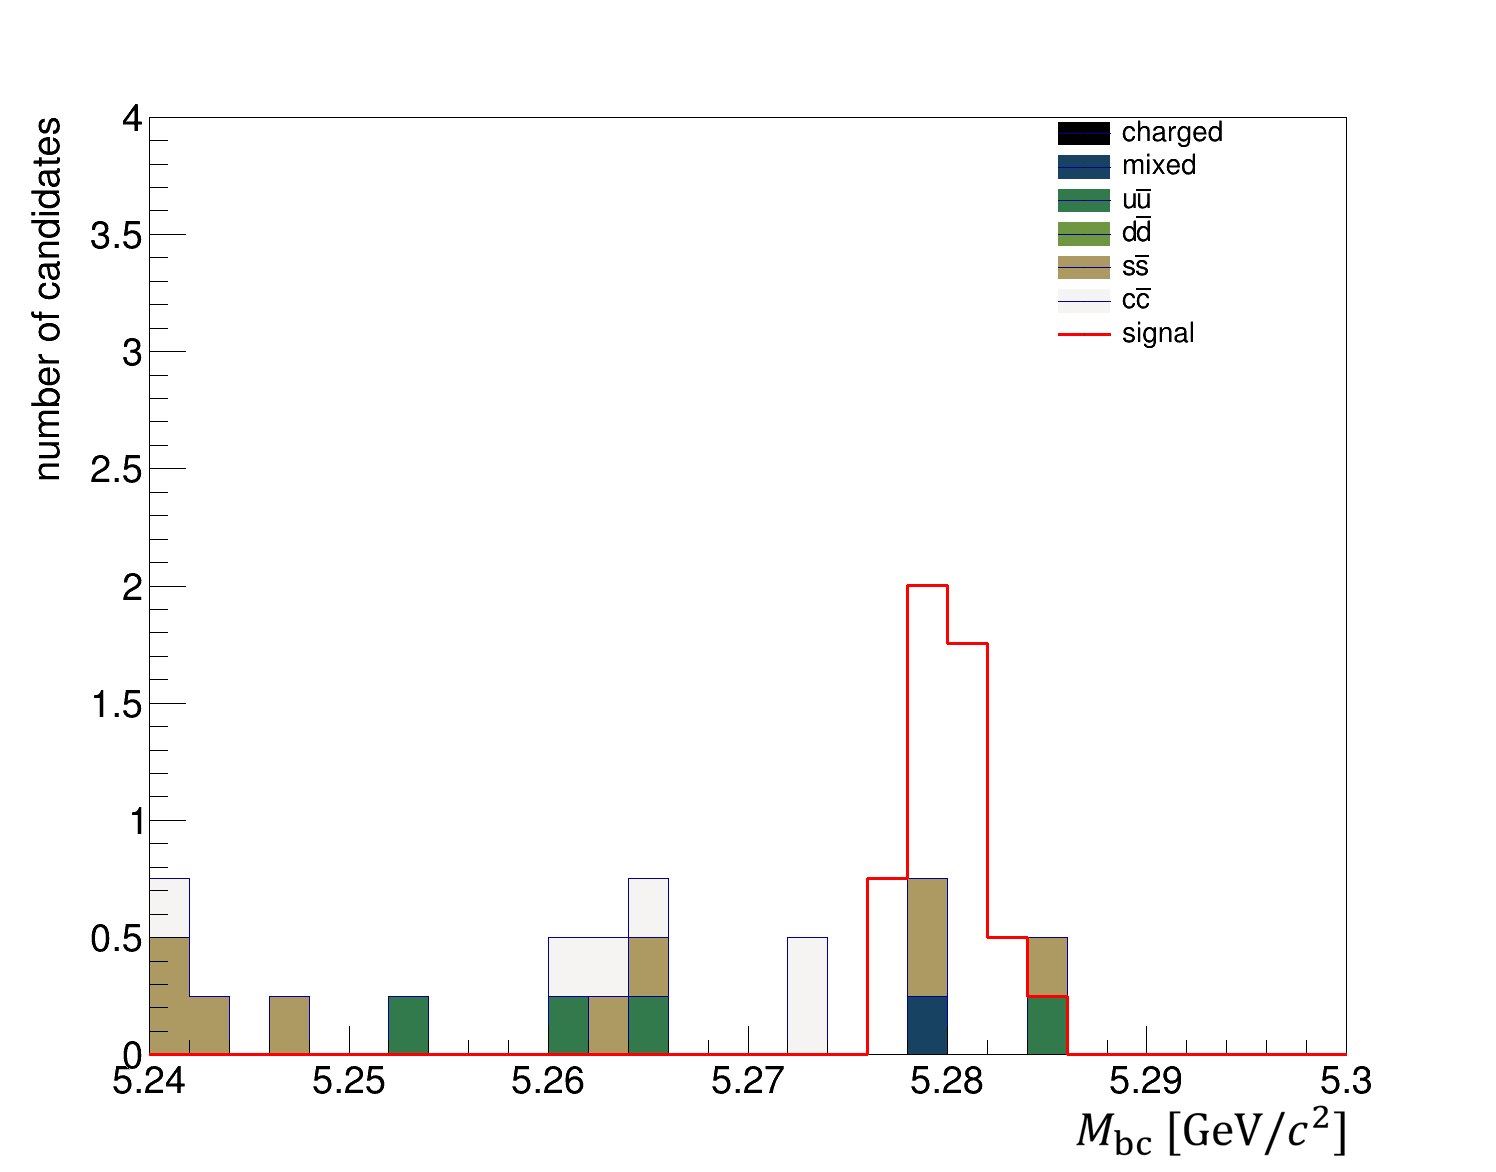
\includegraphics[width=0.6\textwidth]{./picture/KstarKLKL/Plot_Mbc.png}}
  \caption{Distribution of $M_{\textrm{bc}}$ for the $B_{\textrm{sig}}$ candidates in the $B\rightarrow K^{*}K_{S}^{0}K_{S}^{0}$ analysis.}
  \label{fig:Mbc_KstarKLKL}
\end{figure}
One event is observed in data in the region $M_{\textrm{bc}}>5.27~\textrm{GeV}/c^{2}$, with an expected background yield of 1.52 events.
Therefore, an upper limit on the signal yield is determined.
Using the Feldman--Cousins method, the upper limit on the signal yield is 2.90 events at the 90\% confidence level.
The expected signal yield in MC is 3.89 events.
The correction factor is therefore determined to be $2.90/3.89=0.74$.

To reconstruct $B \rightarrow X_{s} K_{S}^{0} K_{S}^{0}$ decay, the $X_{s}$ and $B_{\textrm{tag}}$ candidates are reconstructed using the method described in Section~\ref{sec:rec_and_selec}.
The $X_{s}$ candidate is combined with two $K_{S}^{0}$ candidates to reconstruct $B_{\textrm{sig}}\rightarrow X_{s}K_{S}^{0}K_{S}^{0}$.
After the reconstruction, several cuts are applied. Table~\ref{tab:cutflow_XsKLKL} shows the cut flow for $B \rightarrow X_{s} K_{S}^{0} K_{S}^{0}$ analysis.
Figure~\ref{fig:Mbc_XsKLKL} shows the $M_{\textrm{bc}}$ of $B_{\textrm{sig}}$ distribution after BCS.
\begin{table}
\caption{Cut flow for $B \rightarrow X_{s} K_{S}^{0} K_{S}^{0}$ analysis.}
  \renewcommand{\arraystretch}{1.2}
  \centering
\begin{tabular}{ p{7cm} }
 \hline
  \hline
Selection \\
 \hline
Generated \\
Skim \\
Reconstruction and preselections \\
$M_{bc}>5.2~\textrm{GeV}/c^{2}$ for $B_{\textrm{sig}}$ \\
$\left|\Delta E\right|<0.05~\textrm{GeV}$ for $B_{\textrm{sig}}$\\
$\left|\Delta E\right|<0.2~\textrm{GeV}$ for $B_{\textrm{tag}}$\\
$E_{\textrm{ecl}} < 1.3~\textrm{GeV}$\\
$\texttt{sphericity} > 0.2$\\
$\texttt{R2} < 0.4$ for $B_{\textrm{sig}}$\\
$\texttt{cosTBTO} < 0.9$ for $B_{\textrm{sig}}$\\
$M_{X_{s}} > 1.0~\textrm{GeV}/c^{2}$\\
BCS \\
  \hline
   \hline
\end{tabular}
    \label{tab:cutflow_XsKLKL}
\end{table}
\begin{figure}
  \centering
  \subfloat{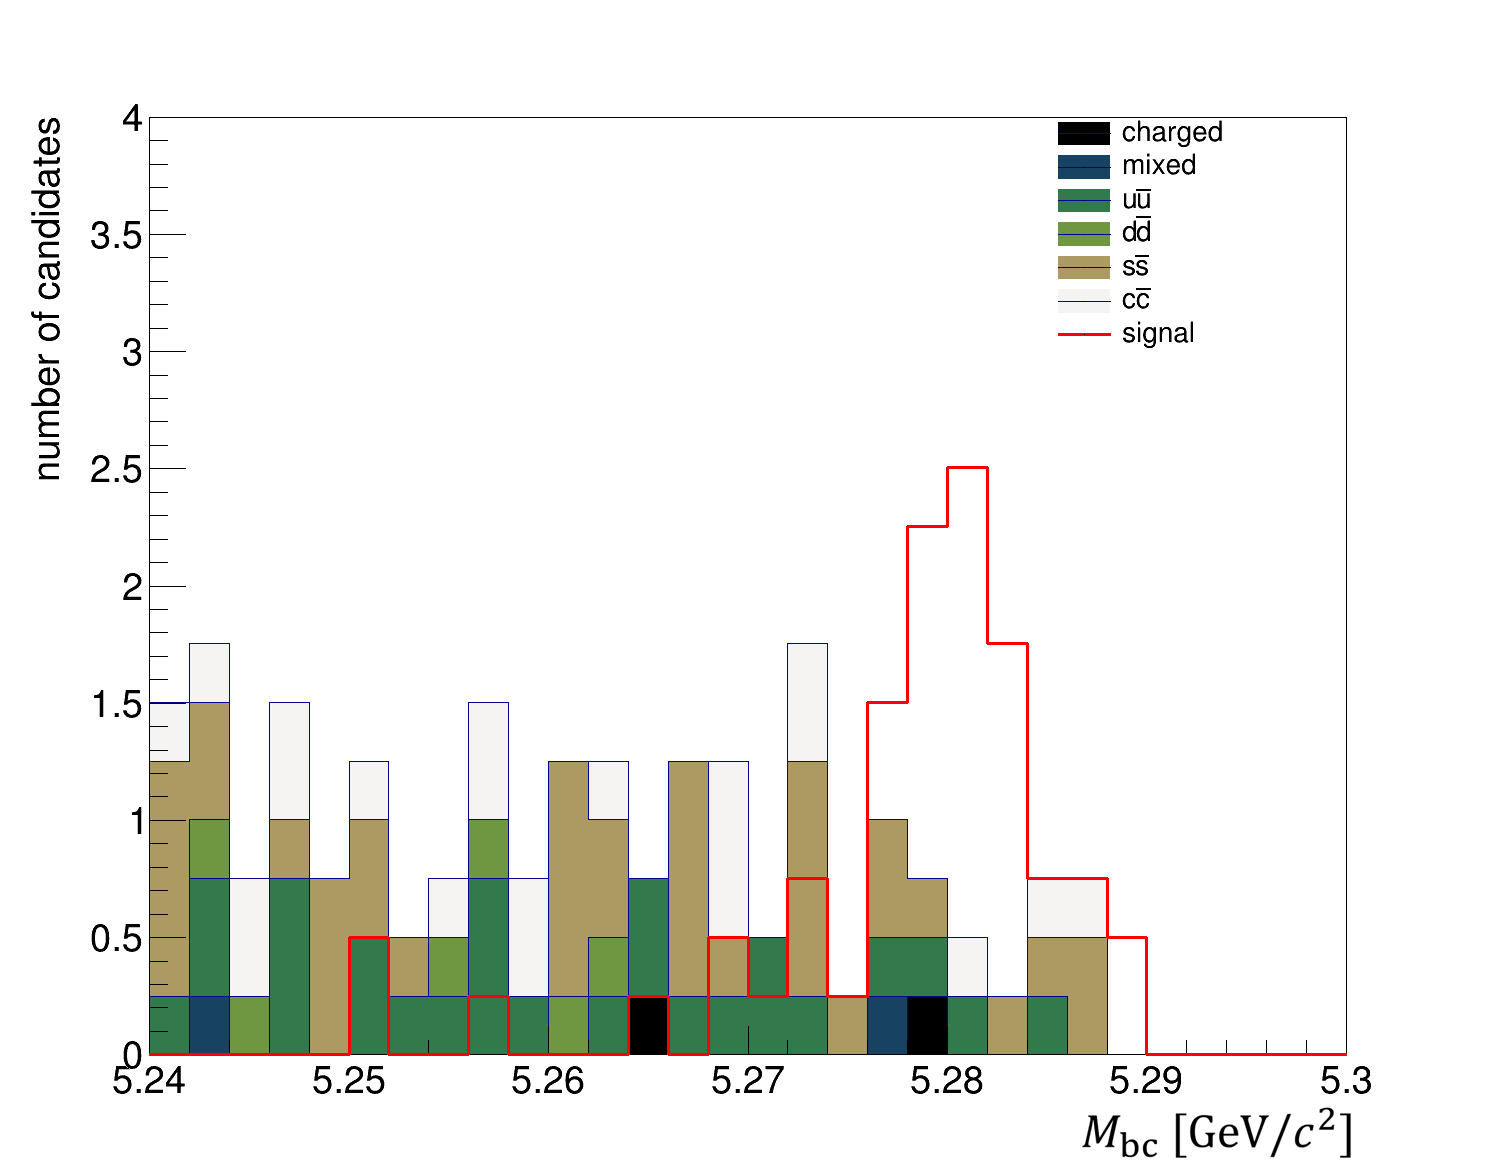
\includegraphics[width=0.6\textwidth]{./picture/XsKLKL/Plot_Mbc.png}}
  \caption{Distribution of $M_{\textrm{bc}}$ for the $B_{\textrm{sig}}$ candidates in the $B\rightarrow X_{s}K_{S}^{0}K_{S}^{0}$ analysis.}
  \label{fig:Mbc_XsKLKL}
\end{figure}
A fit is performed to extract the signal yield.
Table~\ref{tab:function_KSKSbar} summarizes the fit model used in the $B\rightarrow X_{s}K_{S}^{0}K_{S}^{0}$ analysis.
Figure~\ref{fig:KSKS_fit_result} shows the fitting result.
\begin{table}[]
\caption{Fit model used in the $B\rightarrow X_{s}K_{S}^{0}K_{S}^{0}$ analysis.}
\centering
  \begin{tabular}{p{3cm} p{3cm} p{6cm}}
    \hline
    \hline
    Function                    & Parameter &                      \\
    \hline
  \multirow{4}{*}{Crystal Ball} & mean      & fixed using $B \rightarrow K K_{S}^{0} K_{S}^{0}$ data \\
                                & width     & fixed using $B \rightarrow K K_{S}^{0} K_{S}^{0}$ data \\
                                & alpha     & fixed from MC   \\
                                & n         & fixed from MC   \\
                                \hline
  \multirow{3}{*}{ARGUS}        & end point & fixed to the beam energy \\
                                & curvature & floated              \\
                                & power     & fixed to 0.5         \\
  \hline
  \hline
  \end{tabular}
  \label{tab:function_KSKSbar}
\end{table}
\begin{figure}
    \centering
    \subfloat{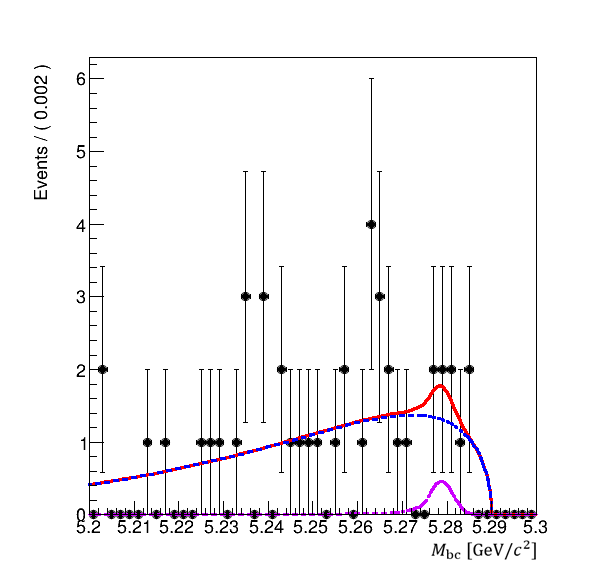
\includegraphics[width=0.4\textwidth]{./picture/XsKLKL/XsKSKS.png}}
    \caption{Fit results for the $B \rightarrow X_{s} K_{S}^{0} K_{S}^{0}$ analysis. The fit variable is $M_{\textrm{bc}}$ of the $B_{\textrm{sig}}$ candidate. The blue curve shows the background component, the purple curve shows the $B \rightarrow X_{s} K_{S}^{0} K_{S}^{0}$ signal component, and the red curve shows their sum.}
    \label{fig:KSKS_fit_result}
\end{figure}
Figure~\ref{fig:XsKSKS_data_MC} shows the comparison between the signal yields extracted from data and those expected from MC.
The blue points show the signal yields extracted from data, and the red points show the expected yields from MC.
The correction factors are defined as the ratios of the data yields to the corresponding MC yields.
\begin{figure}
  \centering
  \subfloat{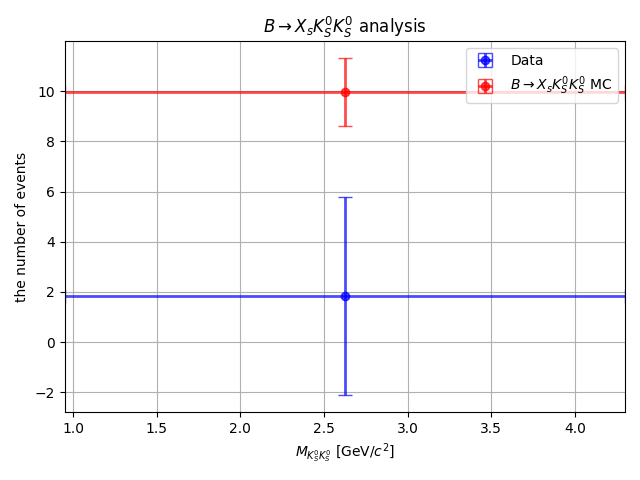
\includegraphics[width=0.6\textwidth]{./picture/XsKLKL/XsKLKL.png}}
  \caption{Comparison of the $M_{K_{S}^{0} K_{S}^{0}}$ distributions in data and MC for $B \rightarrow X_{s} K_{S}^{0} K_{S}^{0}$ decays. The blue points show the signal yields extracted from data, and the red points show the expected yields from MC.}
  \label{fig:XsKSKS_data_MC}
\end{figure}

\section{$D\rightarrow K_{L}^{0}X$ decay from $B$ meson}
\label{sec:DtoKLX_correction}
It was found that the data-MC discrepancy is reduced by applying a scale factor to
$D\rightarrow K_{L}^{0}X$ decays from $B$ mesons~\cite{Belle-II:2023esi}.
In this analysis, a scale factor of $1.3\pm0.1$ is applied.

\chapter{Systematic uncertainties}
\label{sec:systematic_uncertainty}
\section{Tracking efficiency}
The official relative uncertainty of $\pm 0.27\%$ is assigned to each track among the daughters of the $X_{s}$ candidates.
This uncertainty is determined using the tag-and-probe method with $1\times3$-prong $\tau^{+}\tau^{-}$ events in $e^{+}e^{-}\rightarrow \tau^{+}\tau^{-}$ collisions.

\section{Hadron PID}
\label{sec:hadron_pid_syst}
As shown in Appendix~\ref{sec:pid_table}, the PID correction factors and their uncertainties are provided in bins of particle momentum and polar angle.
Because a large number of kinematic bins are used, treating the uncertainty in each PID-correction bin as an independent nuisance parameter would introduce a large number of nuisance parameters into the binned fit.
Furthermore, variations of the correction factors in different PID-correction bins can affect the same fit bins, thereby inducing correlated variations in the predicted yields.

To obtain a compact set of independent systematic variations, principal-component analysis~(PCA) is performed.
A covariance matrix is constructed for the predicted yields across the fit bins and event categories.
The covariance matrix is estimated using toy samples in which the PID correction factors are fluctuated according to their uncertainties.
The covariance matrix is diagonalized as
\begin{equation}
  \Sigma=\sum_{i=1}^{p}\sigma_{i}^{2} \textbf{v}_{i} \textbf{v}_{i}^{T},
\end{equation}
where $\Sigma$ is the covariance matrix, $p$ is its dimension, $\sigma_{i}^{2}$ is the $i$th eigenvalue, and $\textbf{v}_{i}$ is the corresponding eigenvector.
To reduce the number of nuisance parameters, the following approximation is used:
\begin{equation}
  \label{eq:PCA_approximation}
  \Sigma \approx \sum_{i=1}^{t}\sigma_{i}^{2} \textbf{v}_{i} \textbf{v}_{i}^{T} + \textrm{diag} \left( \sum_{i=t+1}^{p}\sigma_{i}^{2} \textbf{v}_{i} \textbf{v}_{i}^{T} \right),
\end{equation}
where $t$ is the number of retained components.
The final diagonal term will be treated as a bin-by-bin uncorrelated uncertainty.
The fraction of the total variance described by the retained components is quantified by the cumulative explained variance ratio:
\begin{equation}
    \frac{\sum_{i=1}^{t}\sigma_{i}^{2}}{\sum_{i=1}^{p}\sigma_{i}^{2}}.
\end{equation}

A total of 500 toy samples are generated to estimate the covariance matrix associated with the \texttt{kaonID} uncertainties.
For each toy sample, the correction factors for the kaon identification efficiency and the pion-to-kaon misidentification rate are fluctuated according to Gaussian distributions.
Figure~\ref{fig:KID_corr} shows the correlation matrices obtained using all eigenvectors and using only the leading 19 eigenvectors.
The cumulative explained variance ratio for these 19 eigenvectors is $0.96$.
The leading 19 eigenvectors are retained and implemented as independent nuisance parameters in the fit.

The same procedure is applied to the \texttt{pionID} uncertainties.
A total of 500 toy samples are generated by fluctuating the correction factors for the pion identification efficiency and the kaon-to-pion misidentification rate.
Figure~\ref{fig:PID_corr} shows the correlation matrices obtained using all eigenvectors and using only the leading 19 eigenvectors.
The cumulative explained variance ratio for these 19 eigenvectors is $0.96$.
The leading 19 eigenvectors are retained and implemented as independent nuisance parameters in the fit.
\begin{figure}
    \centering
    \subfloat[][Correlation matrix among the fit bins and event categories
    induced by the \texttt{kaonID} uncertainties.]
    {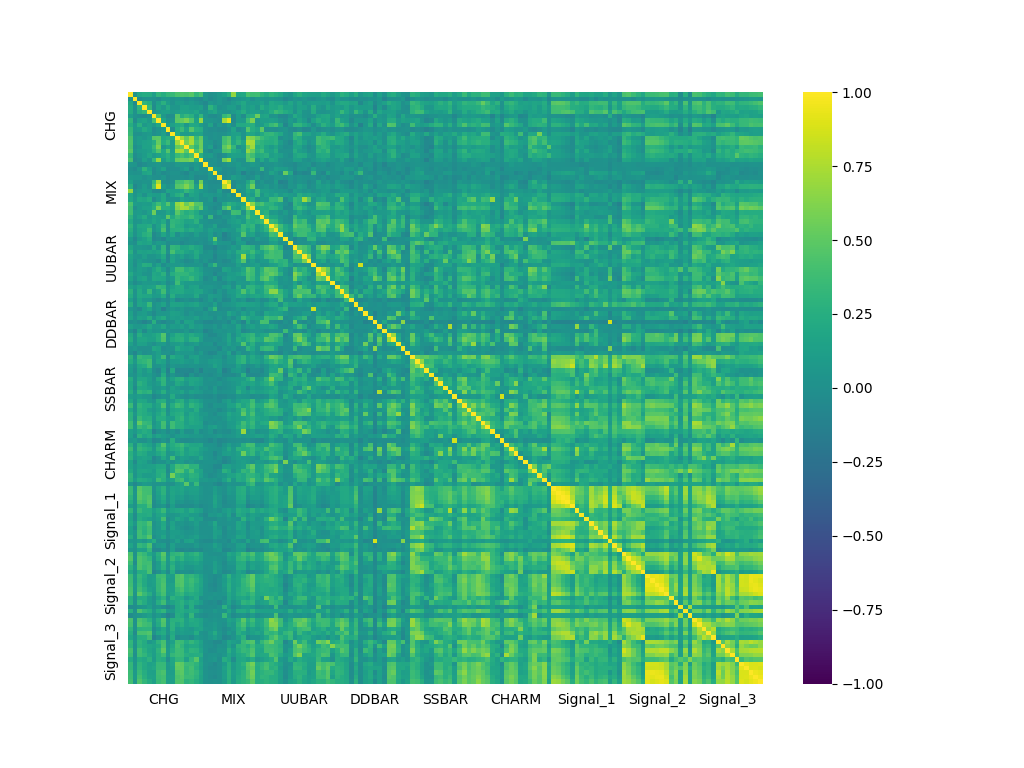
\includegraphics[width=0.45\textwidth]
    {./picture/systematic/KID_corr_all.png}}
    \hfill
    \subfloat[][Correlation matrix reconstructed using the leading
    19 eigenvectors.]
    {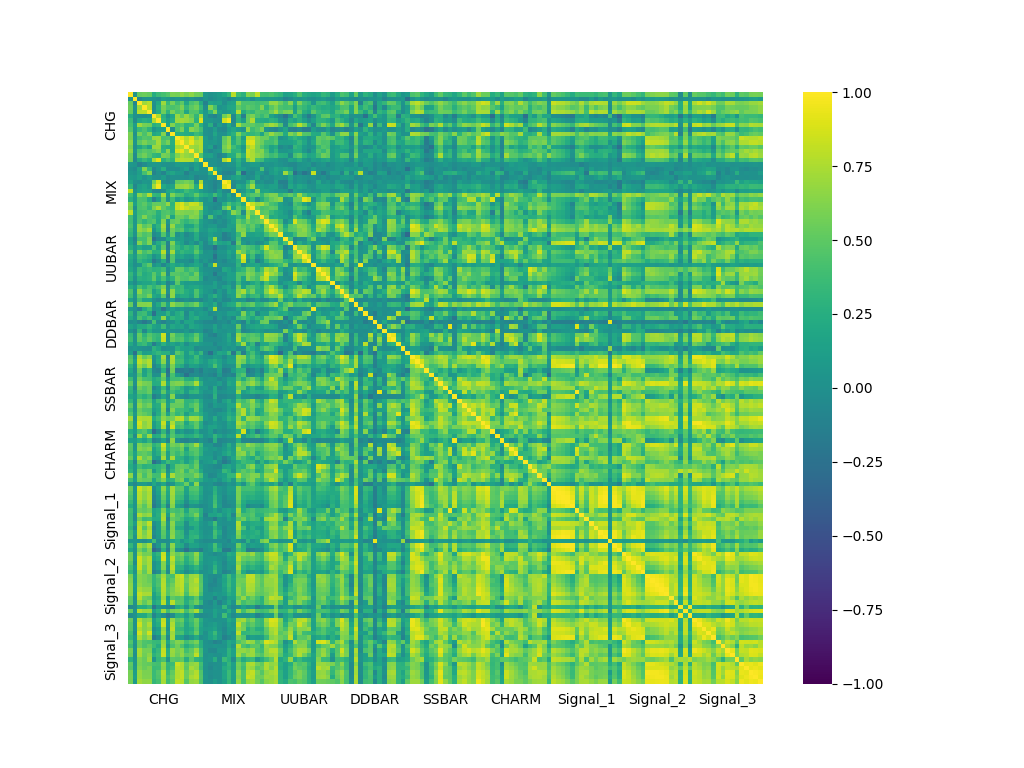
\includegraphics[width=0.45\textwidth]
    {./picture/systematic/KID_corr_partial.png}}
    \caption{
    Correlation matrices associated with the \texttt{kaonID} systematic
    uncertainty.
    The left plot is obtained using all eigenvectors, while the right plot
    is reconstructed using the leading 19 eigenvectors.
    }
    \label{fig:KID_corr}
\end{figure}
\begin{figure}
    \centering
    \subfloat[][Correlation matrix among the fit bins and event categories
    induced by the \texttt{pionID} uncertainties.
    White regions correspond to bins with no pion candidates and therefore no yield variation induced by the \texttt{pionID} uncertainties.]
    {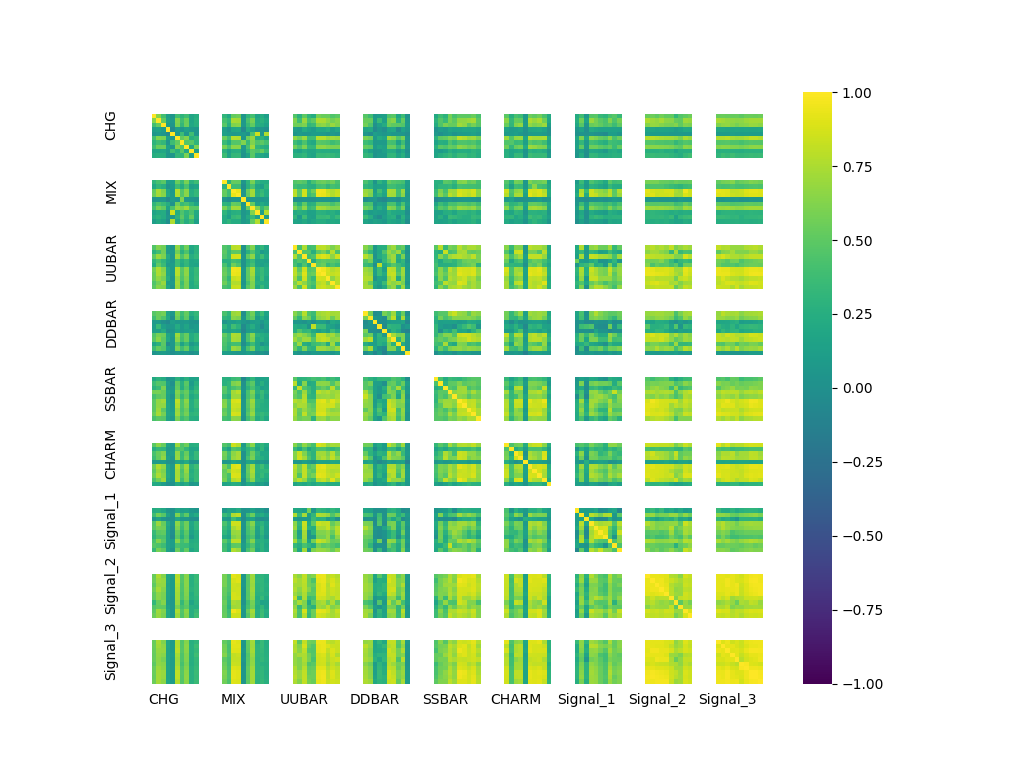
\includegraphics[width=0.45\textwidth]{./picture/systematic/PID_corr_all.png}}
    \hfill
    \subfloat[][Correlation matrix reconstructed using the leading
    19 eigenvectors.]
    {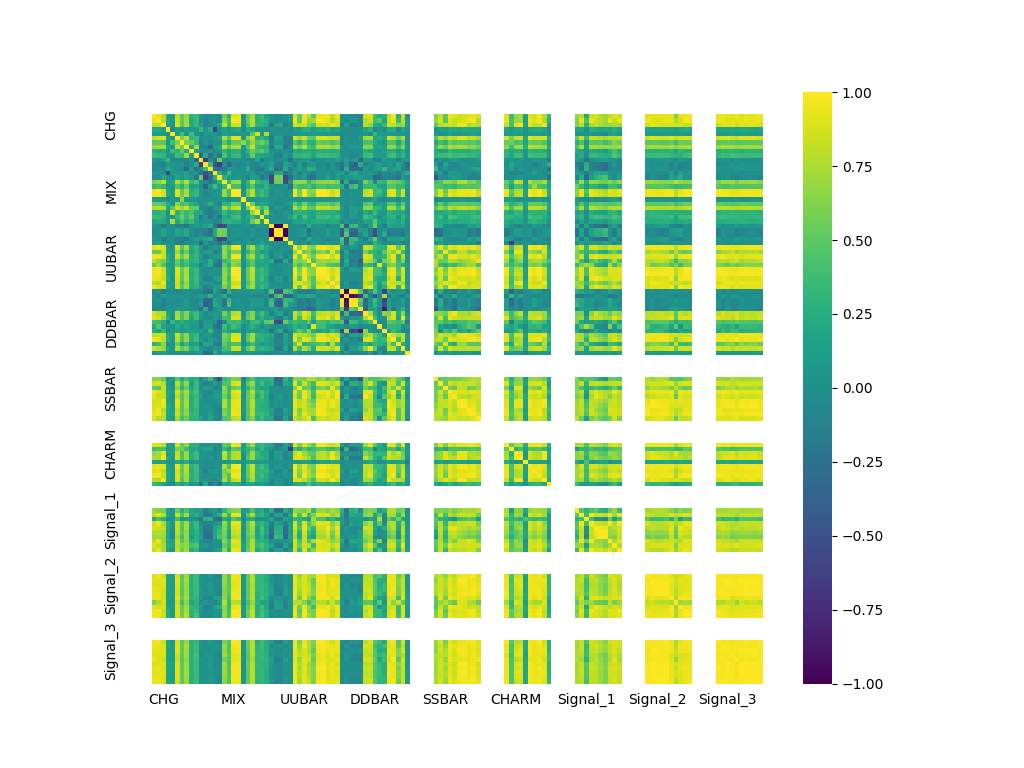
\includegraphics[width=0.45\textwidth]{./picture/systematic/PID_corr_partial.png}}
    \caption{
    Correlation matrices associated with the \texttt{pionID} systematic
    uncertainty.
    The left plot is obtained using all eigenvectors, while the right plot
    is reconstructed using the leading 19 eigenvectors.
    }
    \label{fig:PID_corr}
\end{figure}

\section{$K_{S}^{0}$ efficiency}
The official uncertainty associated with the $K_{S}^{0}$ efficiency correction factor, discussed in Section~\ref{sec:KS0_eff_corr}, is used.
The same procedure described in Section~\ref{sec:hadron_pid_syst} is used to reduce the number of nuisance parameters.

A total of 500 toy samples are generated to estimate the covariance matrix associated with the $K_{S}^{0}$ efficiency uncertainty.
For each toy sample, the $K_{S}^{0}$ efficiency correction factors are varied according to Gaussian distributions defined by their uncertainties.

Figure~\ref{fig:KS0_corr} shows the correlation matrices obtained using all
eigenvectors and using only the leading four eigenvectors.
The cumulative explained variance ratio for these 4 eigenvectors is 0.97.
The leading 4 eigenvectors are retained and implemented as independent nuisance parameters in the fit.
\begin{figure}
    \centering
    \subfloat[][Correlation matrix among the fit bins and event categories
    induced by the $K_{S}^{0}$ efficiency uncertainties.
    White regions correspond to bins with no $K_{S}^{0}$ candidates and therefore no yield variation induced by the $K_{S}^{0}$ efficiency uncertainties.]{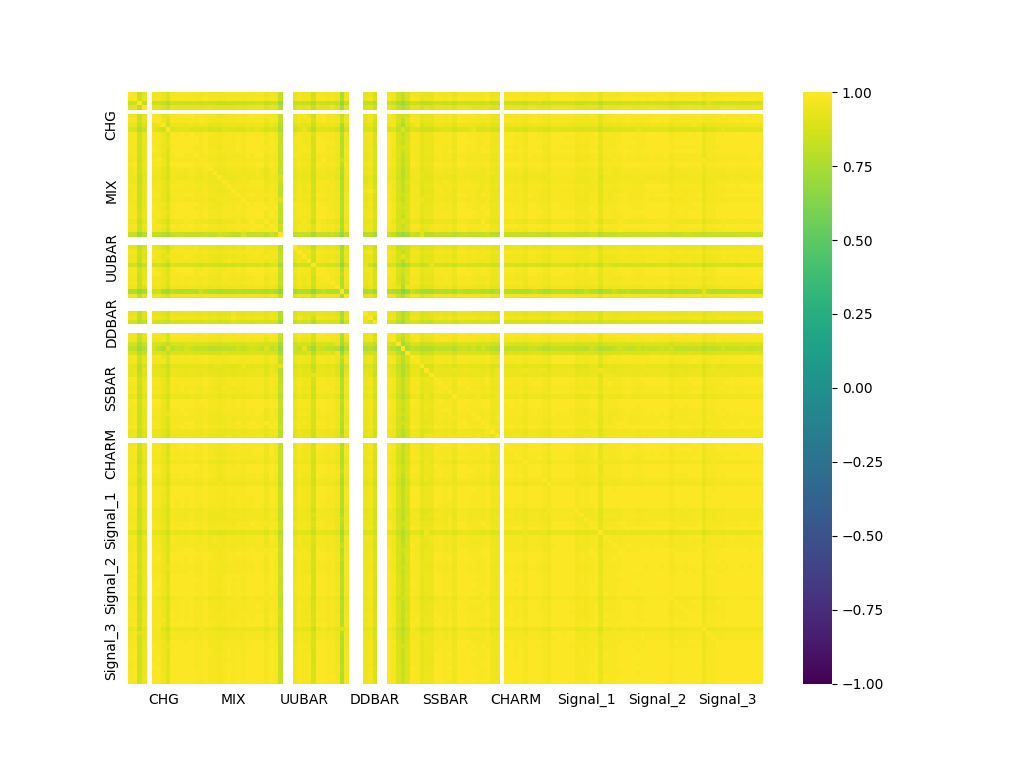
\includegraphics[width=0.45\textwidth]{./picture/systematic/KS0_corr_all.png}}
    \hfill
    \subfloat[][Correlation matrix reconstructed using the leading four eigenvectors.]{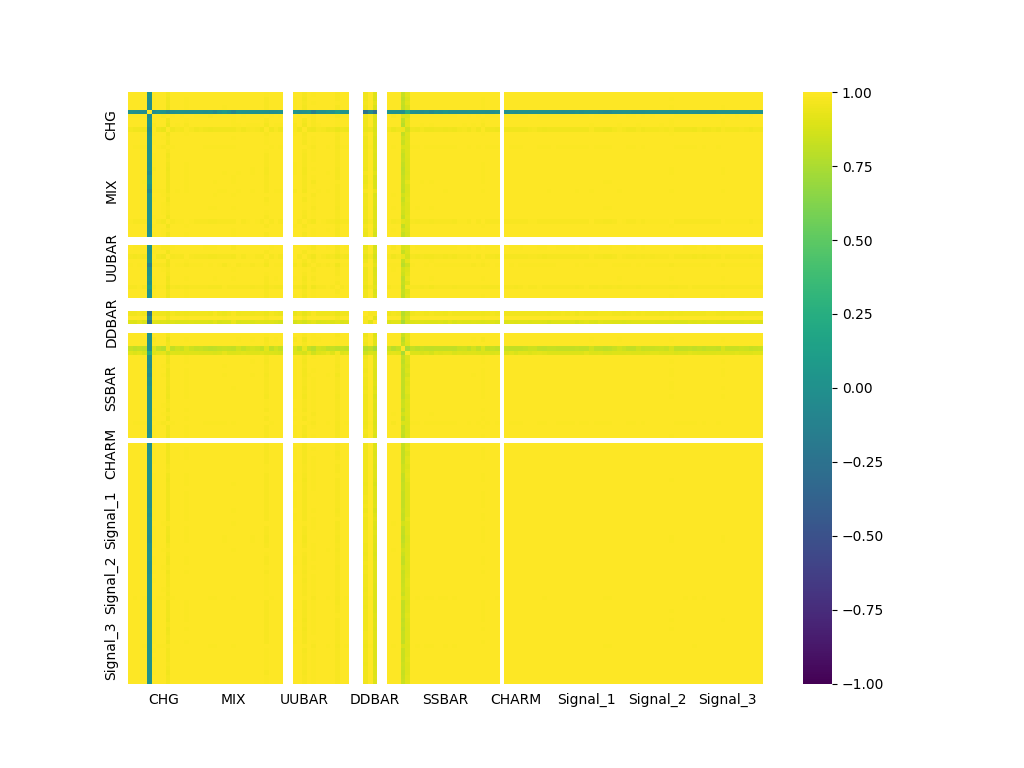
\includegraphics[width=0.45\textwidth]{./picture/systematic/KS0_corr_partial.png}}
    \caption{Correlation matrices associated with the $K_{S}^{0}$ efficiency
    systematic uncertainty. The left plot is obtained using all eigenvectors, while the right plot is reconstructed using the leading four eigenvectors.}
    \label{fig:KS0_corr}
\end{figure}

\section{$\pi^{0}$ efficiency}
The official uncertainty associated with the $\pi^{0}$ efficiency correction factor, discussed in Section~\ref{sec:pi0_eff_corr}, is used.
The same procedure described in Section~\ref{sec:hadron_pid_syst} is used to reduce the number of nuisance parameters.

A total of 500 toy samples are generated to estimate the covariance matrix associated with the $\pi^{0}$ efficiency uncertainty.
For each toy sample, the $\pi^{0}$ efficiency correction factors are varied according to Gaussian distributions defined by their uncertainties.

Figure~\ref{fig:pi0_corr} shows the correlation matrices obtained using all
eigenvectors and using only the leading four eigenvectors.
The cumulative explained variance ratio for these 7 eigenvectors is 0.96.
The leading 7 eigenvectors are retained and implemented as independent nuisance parameters in the fit.
\begin{figure}
    \centering
    \subfloat[][Correlation matrix among the fit bins and event categories
    induced by the $\pi^{0}$ efficiency uncertainties.
    White regions correspond to bins with no $\pi^{0}$ candidates and therefore no yield variation induced by the $\pi^{0}$ efficiency uncertainties.]{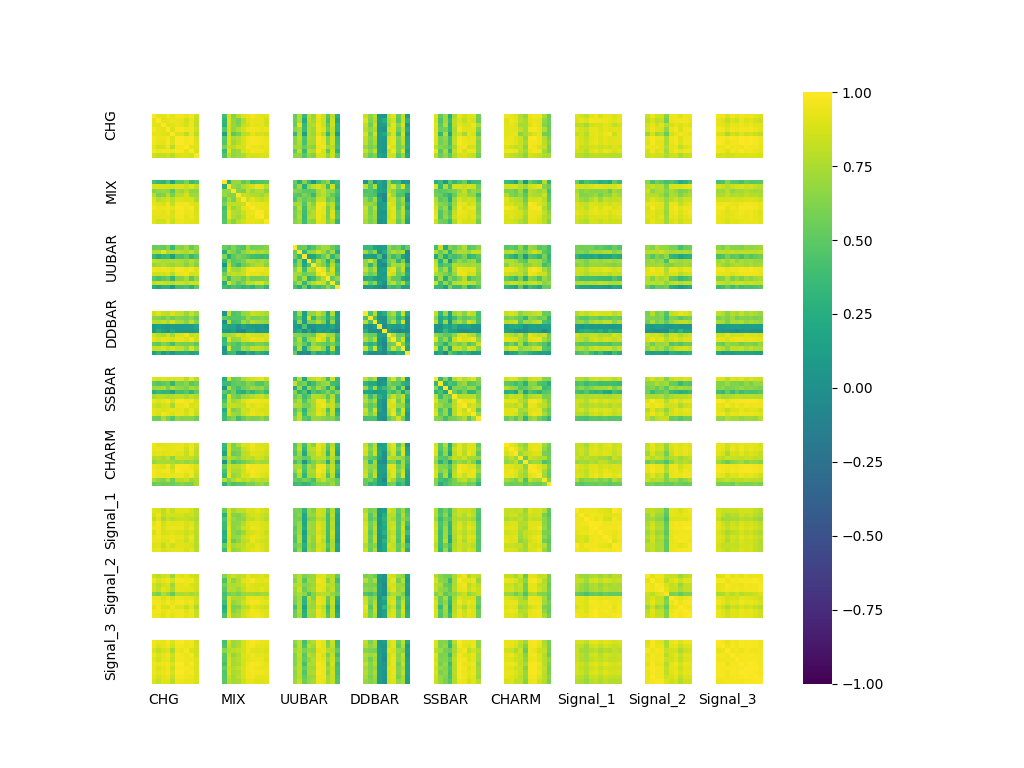
\includegraphics[width=0.45\textwidth]{./picture/systematic/pi0_corr_all.png}}
    \hfill
    \subfloat[][Correlation matrix reconstructed using the leading 7 eigenvectors.]{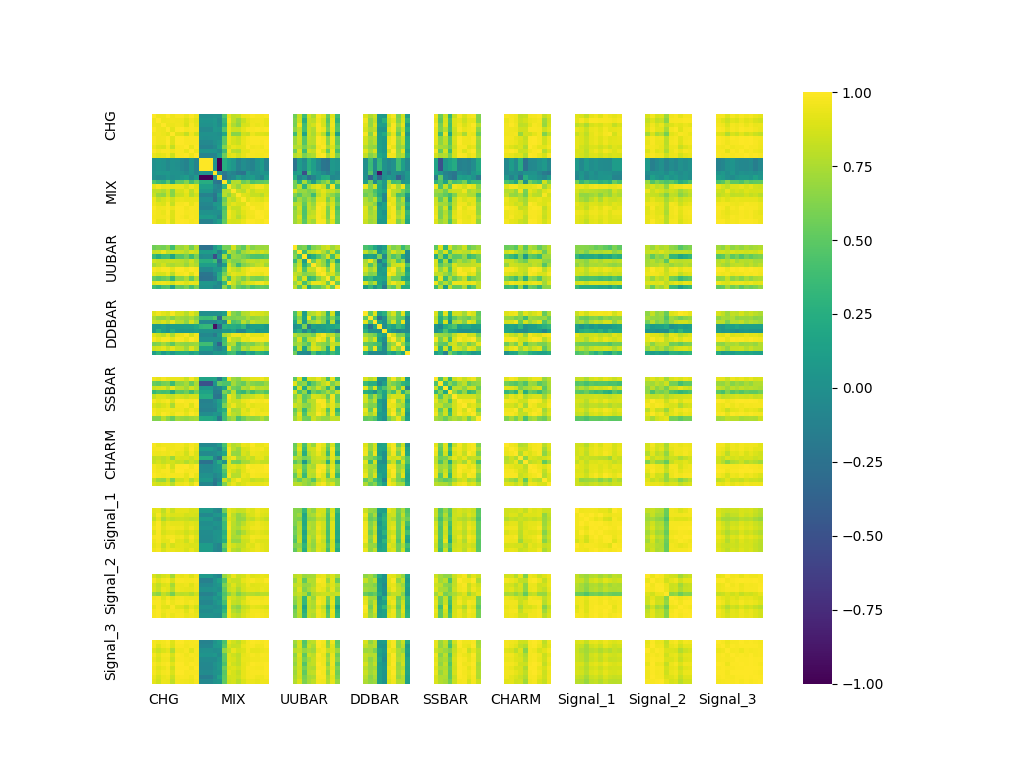
\includegraphics[width=0.45\textwidth]{./picture/systematic/pi0_corr_partial.png}}
    \caption{Correlation matrices associated with the $\pi^{0}$ efficiency
    systematic uncertainty.The left plot is obtained using all eigenvectors, while the right plot is reconstructed using the leading 7 eigenvectors.}
    \label{fig:pi0_corr}
\end{figure}

\section{FastBDT efficiency}
The $B \rightarrow X_{s} J/\psi$ control-sample study is described in Section~\ref{sec:control_sample}.
The uncertainties in the data-to-MC ratios of the FastBDT selection efficiency given in Eq.~\ref{eq:FBDT_efficiency_ratio_data_MC_XsJpsi} are assigned as systematic uncertainties.

\section{Form Factors for $B \rightarrow K^{(*)} \nu \bar{\nu}$}
\label{subsec:formfactor_uncertainty}
The decay amplitudes for $B\rightarrow K\nu\bar{\nu}$ and $B\rightarrow K^{*}\nu\bar{\nu}$ depend on the form factors given in Eqs.~\ref{eq:Kamp} and~\ref{eq:Kstaramp}.
These form factors have uncertainties arising from the parameters of the $z$ expansion given in Eqs.~\ref{eq:coeff_Kff} and~\ref{eq:Kstnunu_alpha}.

The form-factor parameters are varied, and the resulting changes in the predicted event yields in the fit bins are evaluated.
These yield variations are treated as systematic uncertainties.

Because the form-factor parameters are correlated~\cite{Parrott:2022rgu,Bharucha:2015bzk}, PCA is performed to obtain independent variation directions.
The parameters are varied along the resulting eigenvectors.

\section{FEI calibration for $B\bar{B}$}
As discussed in Section~\ref{sec:FEI_calibration}, the official FEI calibration factors are applied.
These calibration factors have associated uncertainties and correlations among the $B_{\textrm{tag}}$ decay channels.
The covariance matrix of the FEI calibration factors is diagonalized using PCA, and the resulting eigenvectors define independent variation directions.

A total of 500 toy samples are generated by varying the FEI calibration factors along these eigenvector directions according to their uncertainties.
For each toy sample, the predicted event yields in the fit bins are recalculated.
A covariance matrix of the predicted yields across the fit bins is then constructed from the toy samples.

The same procedure described in Section~\ref{sec:hadron_pid_syst} is applied to this yield covariance matrix to reduce the number of nuisance parameters.
Figure~\ref{fig:FEI_corr} shows the correlation matrices reconstructed using all eigenvectors and using only the leading three eigenvectors.
The cumulative explained variance ratio for these three eigenvectors is 0.98.
The leading three eigenvectors are retained and implemented as independent nuisance parameters in the fit.
\begin{figure}
  \centering
  \subfloat[][Correlation matrix among the fit bins and event categories induced by the FEI calibration uncertainties.]{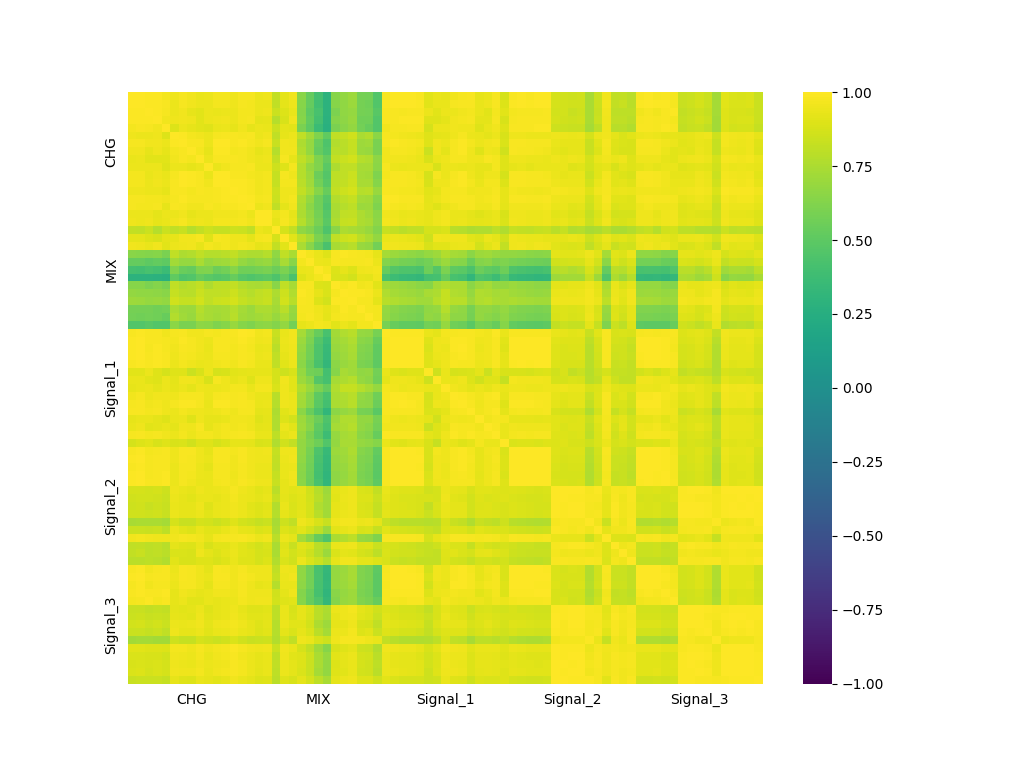
\includegraphics[width=0.45\textwidth]{./picture/systematic/FEI_corr_all.png}}
  \hfill
  \subfloat[][Correlation matrix reconstructed using the leading three eigenvectors.]{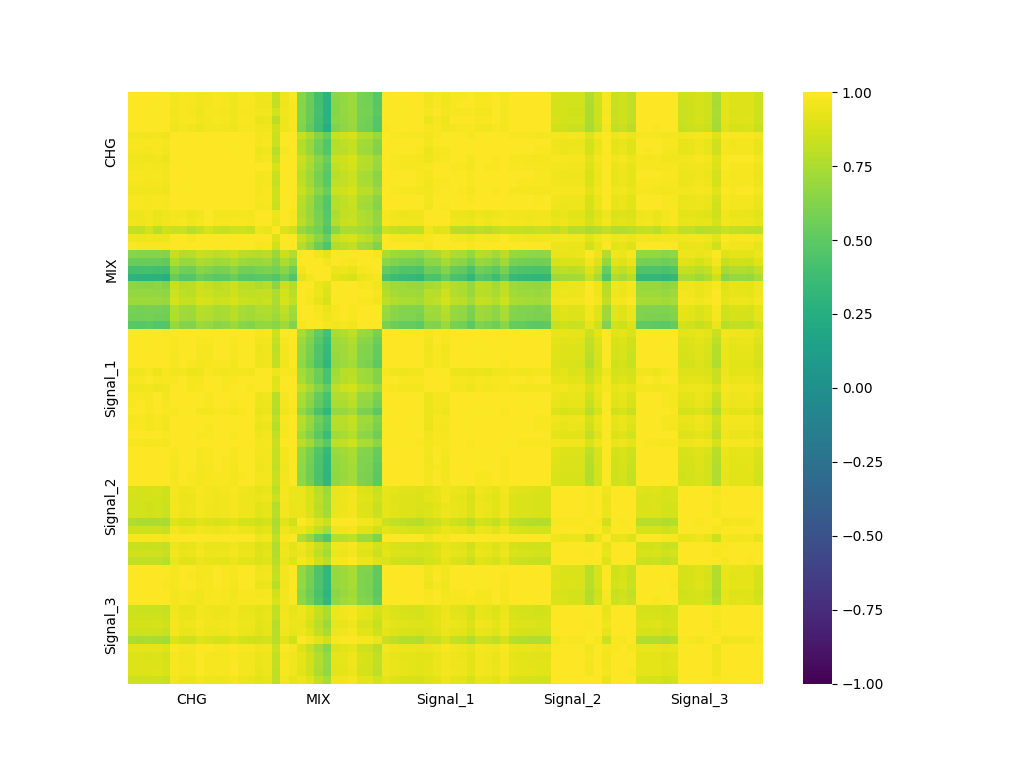
\includegraphics[width=0.45\textwidth]{./picture/systematic/FEI_corr_partial.png}}
  \caption{Correlation matrices associated with the FEI calibration systematic uncertainty. The left plot is obtained using all eigenvectors, while the right plot is reconstructed using the leading three eigenvectors.}
  \label{fig:FEI_corr}
\end{figure}

\section{Additional uncertainty in the FEI calibration}
As discussed in Section~\ref{sec:FEI_calibration}, the official FEI efficiency calibration factors are applied.
These factors are derived using $B\rightarrow X\ell\nu$ decays.
As an additional study, a possible dependence of the FEI calibration on the signal-side decay topology and cut flow is investigated using $B\rightarrow K^{(*)}J/\psi$ decays.

The control-sample analysis described in Section~\ref{sec:control_sample} is used.
However, the $X_{s}$ candidate is required to be reconstructed in either a $K$ or $K\pi$ final state with $M_{X_{s}}<1.0~\textrm{GeV}/c^{2}$.
Figure~\ref{fig:another_FEI_charged} shows the event yields in data and MC for the different $B_{\textrm{tag}}$ decay channels.
\begin{figure}
  \centering
  \subfloat[][Charged $B_{\textrm{tag}}$]
  {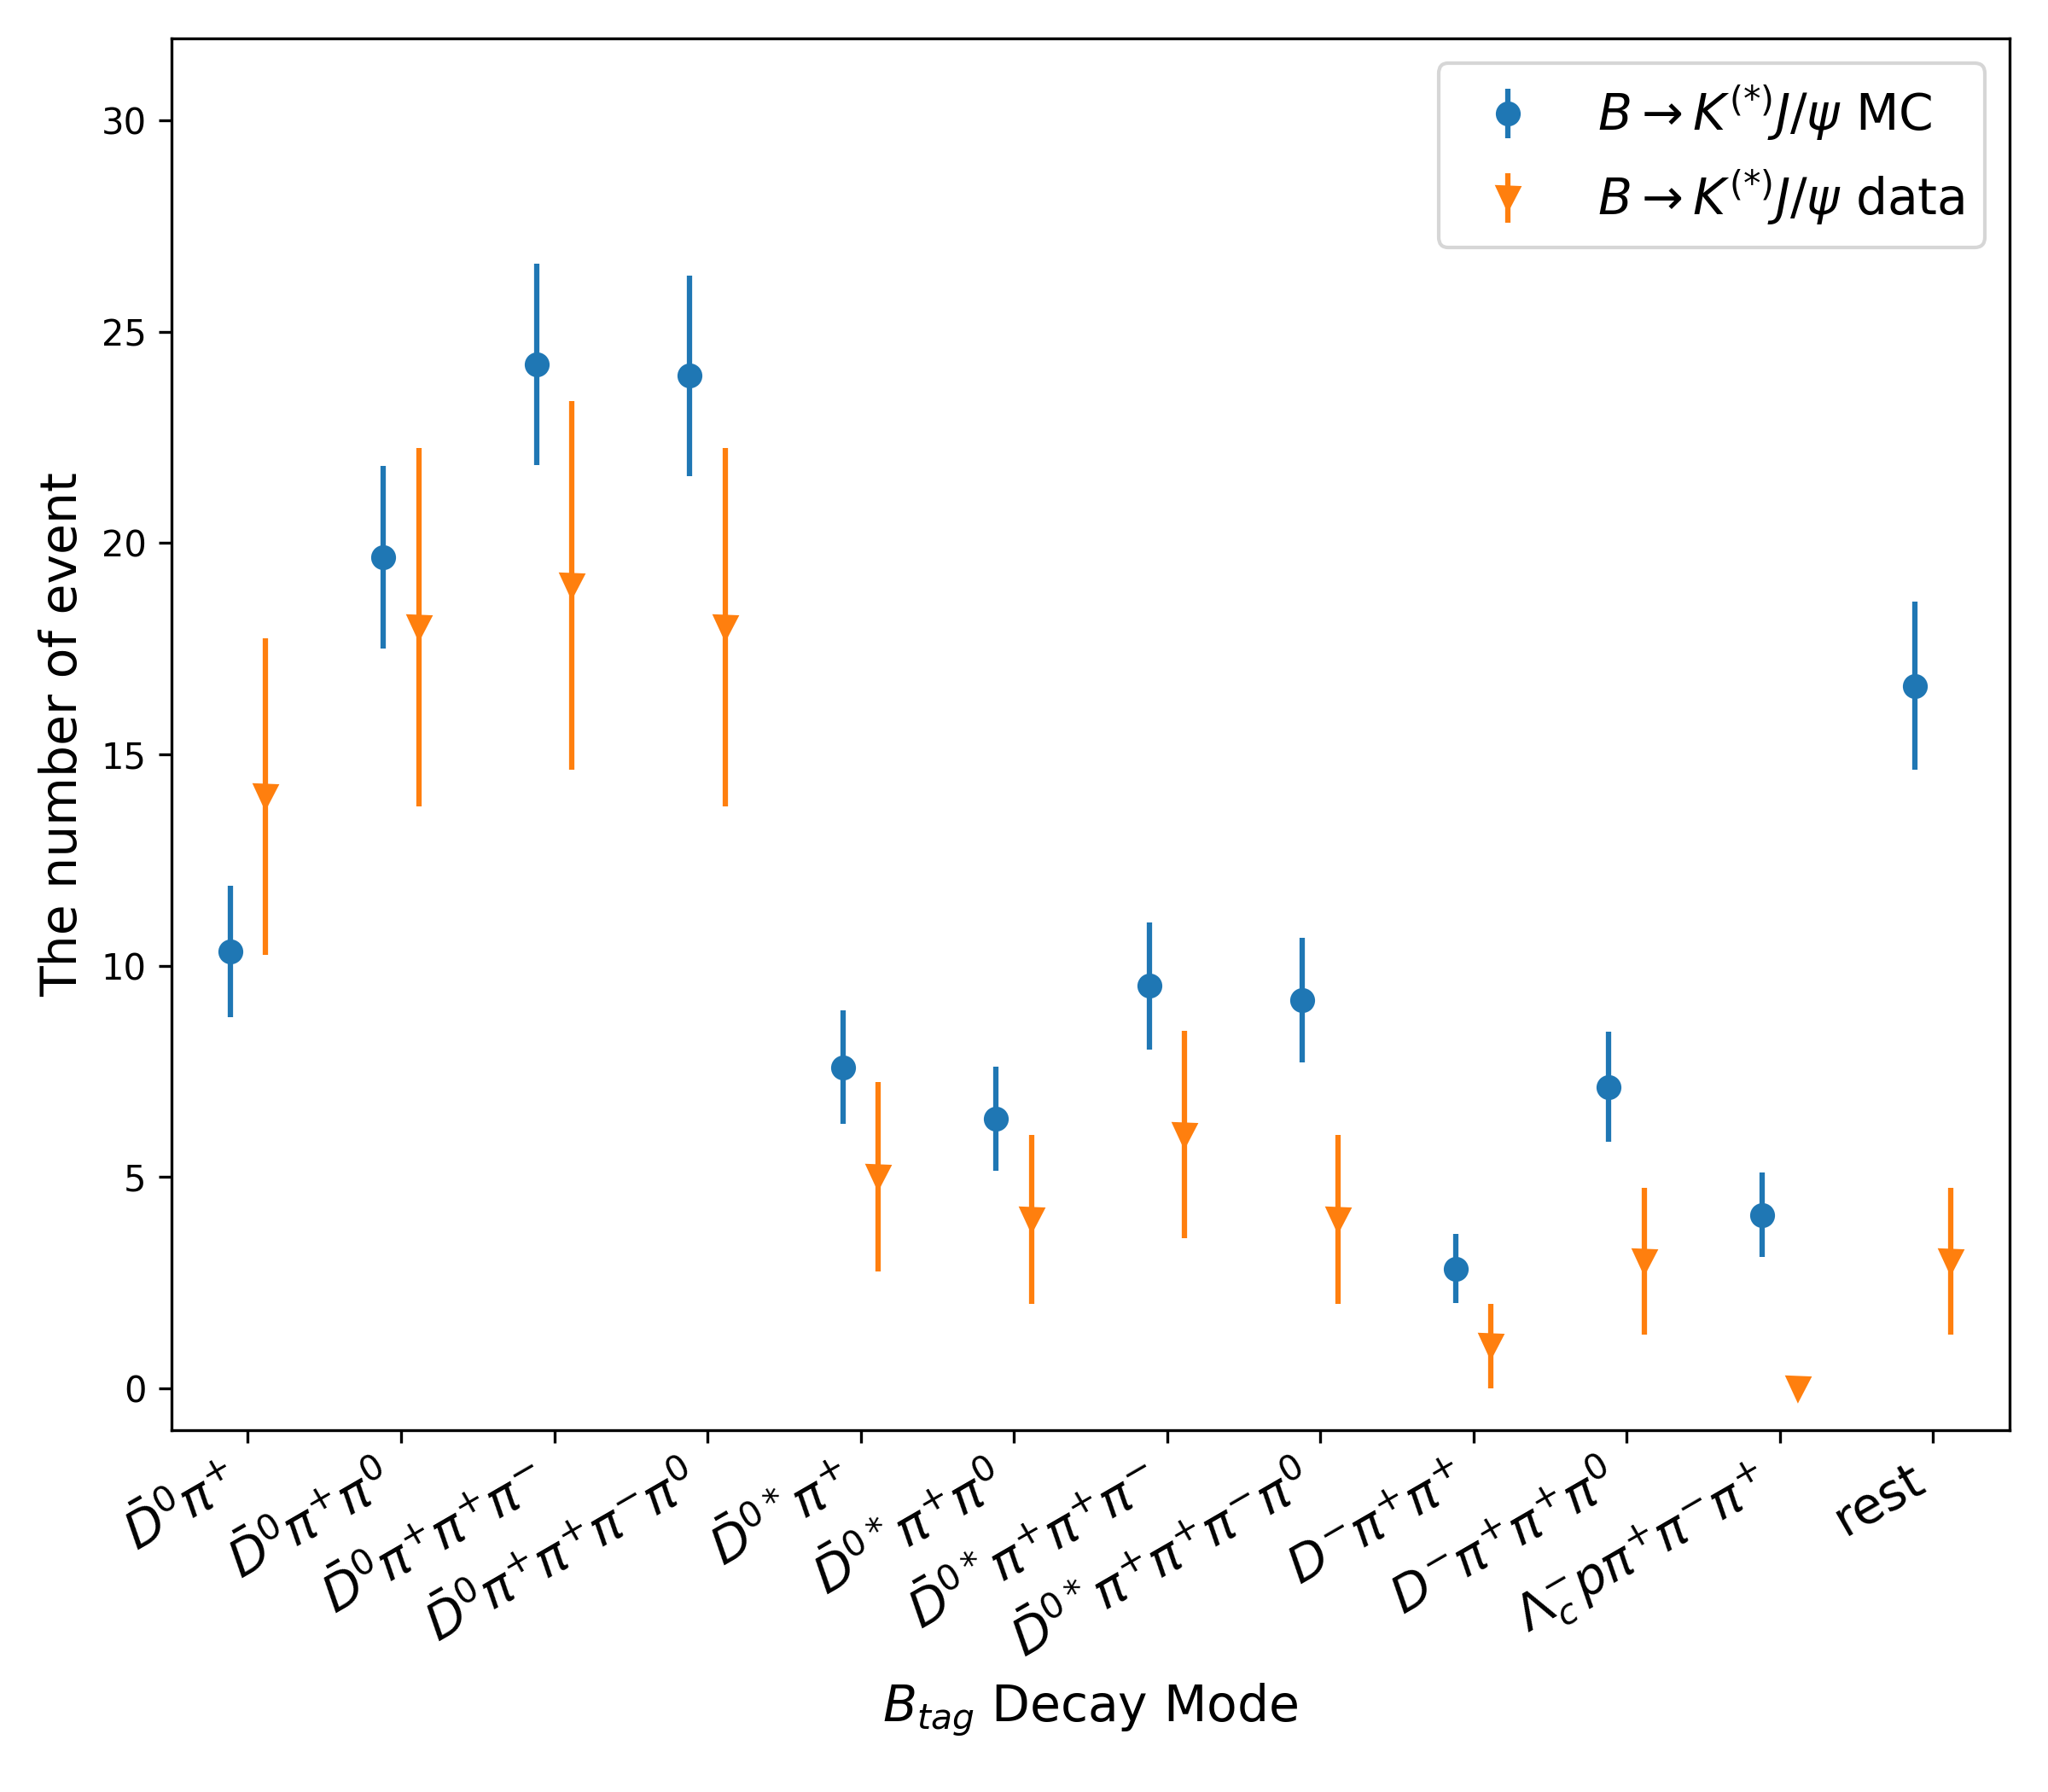
\includegraphics[width=0.45\textwidth]{./picture/systematic/Number_of_event_comparison_Bplus.png}}
  \hfill
  \subfloat[][Neutral $B_{\textrm{tag}}$]
  {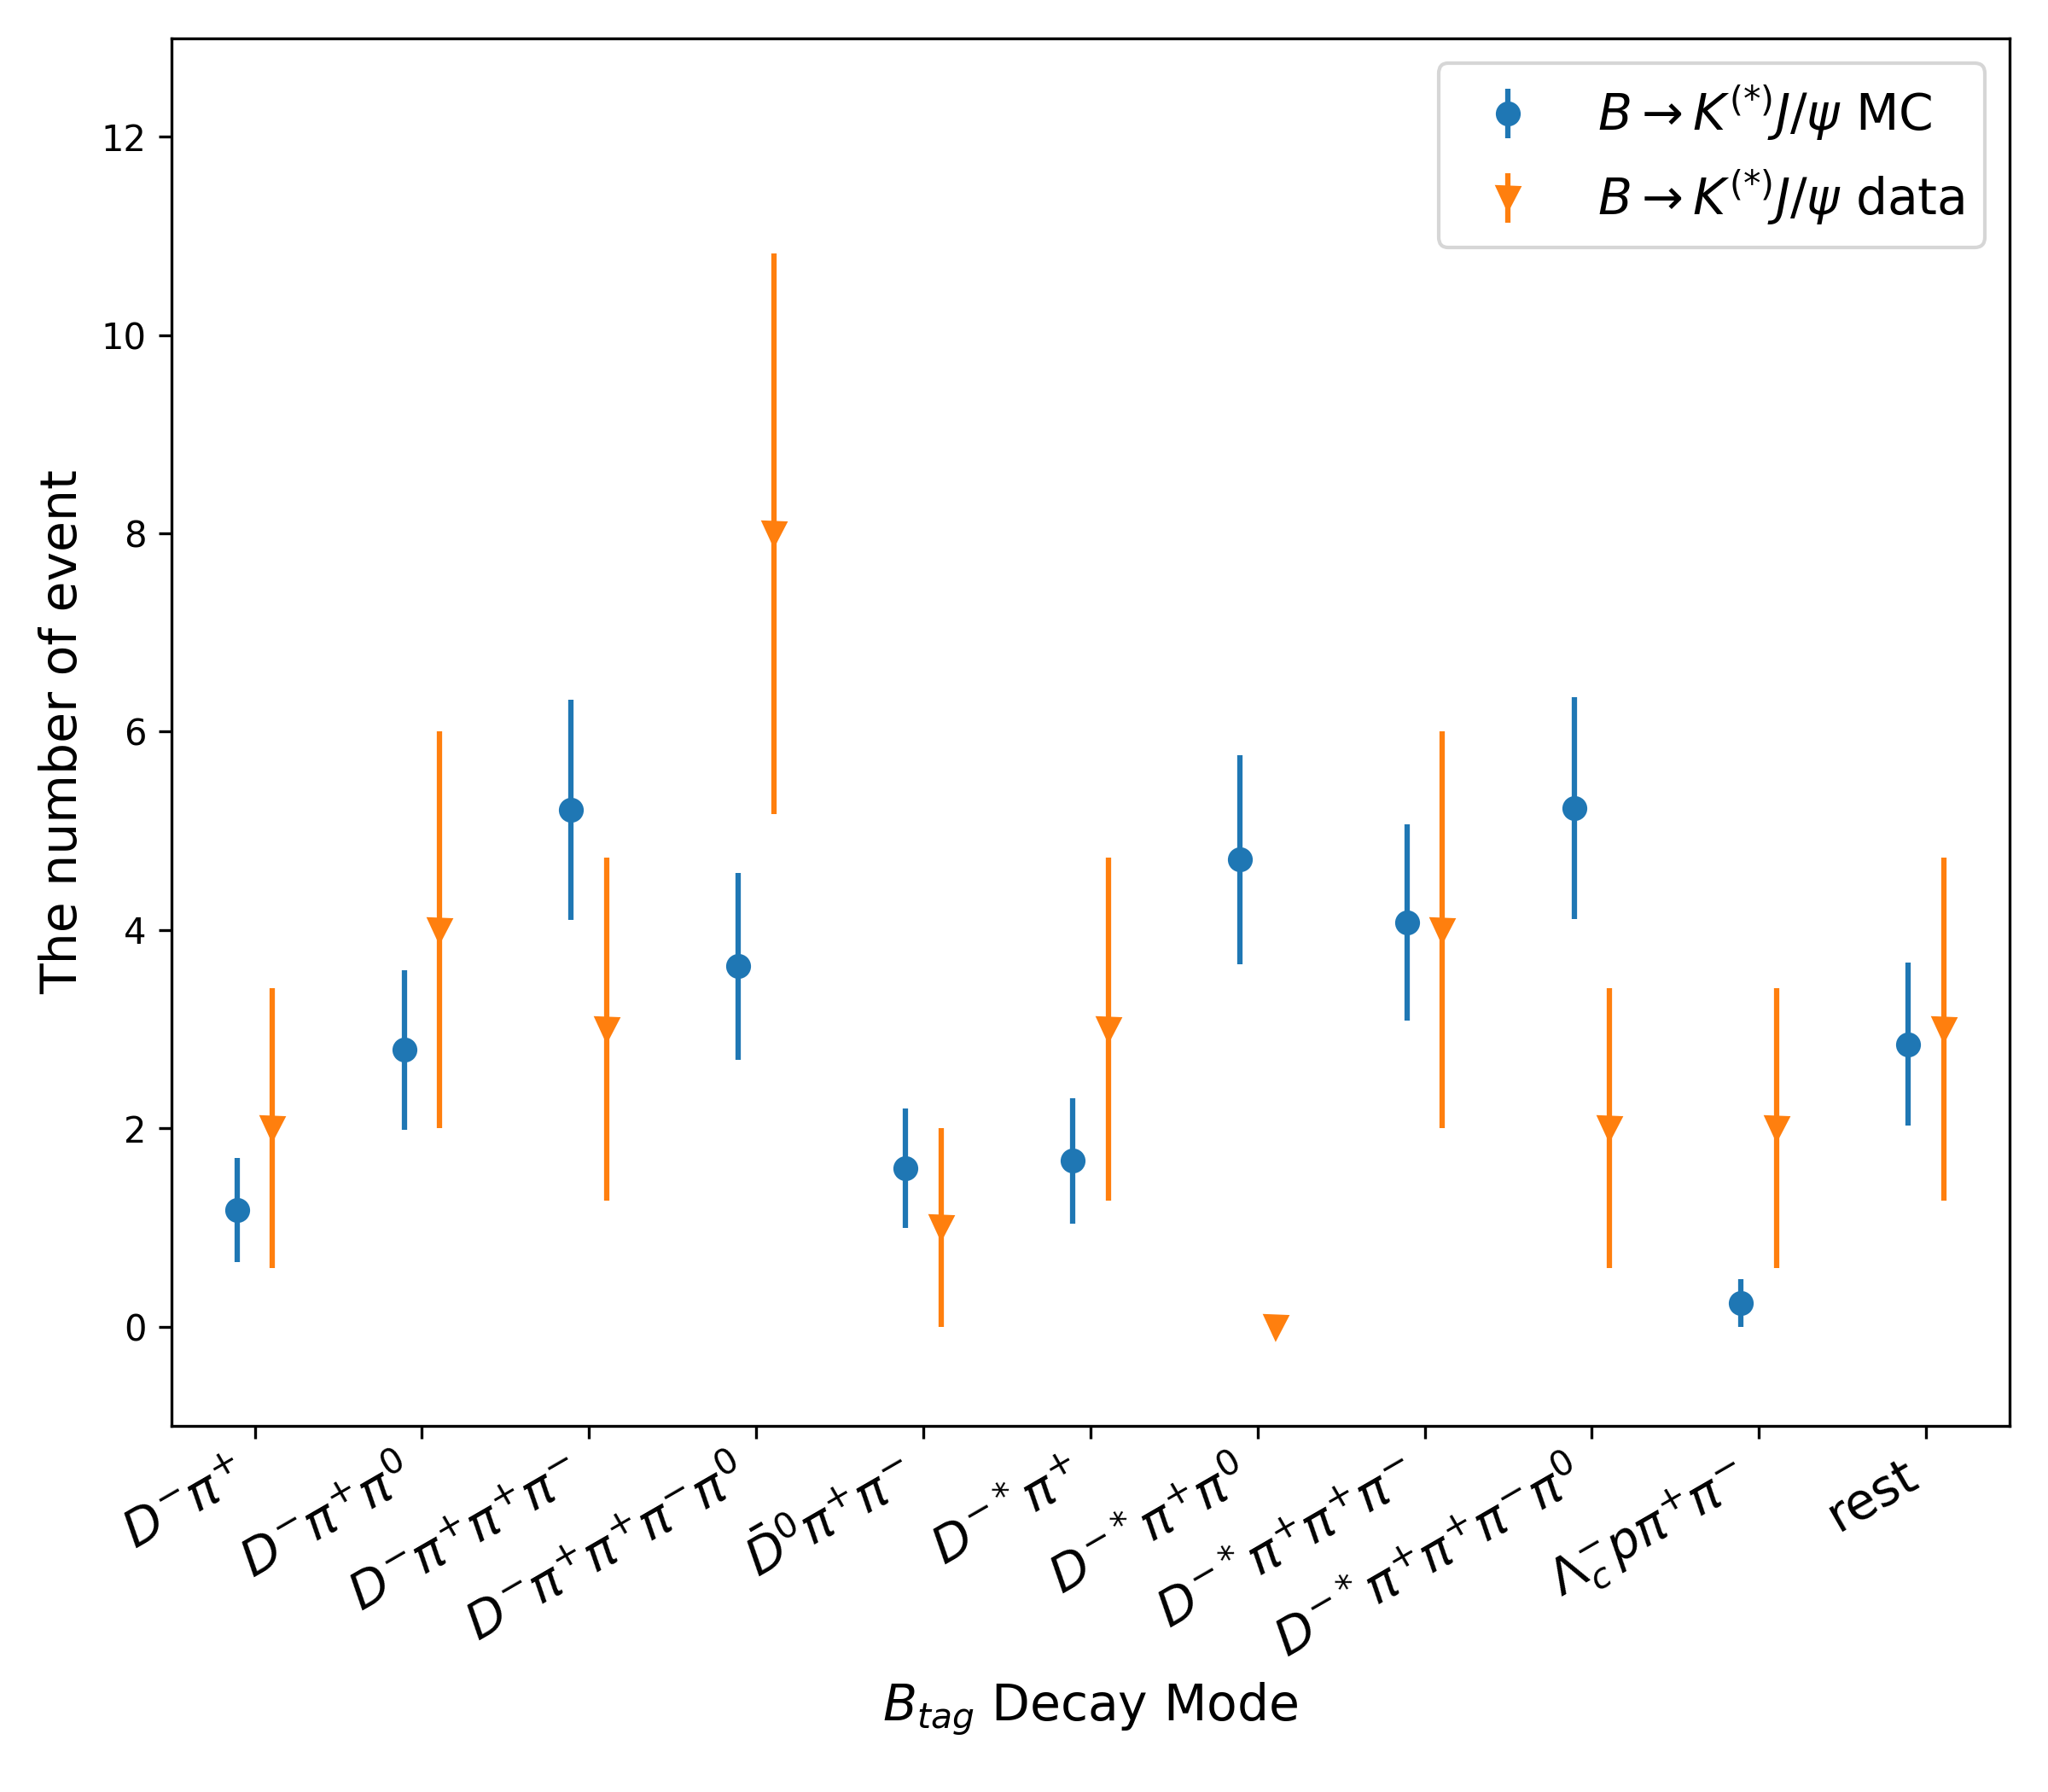
\includegraphics[width=0.45\textwidth]{./picture/systematic/Number_of_event_comparison_Bzero.png}}
  \caption{
  Comparison of the event yields in data and MC for $B\rightarrow K^{(*)}J/\psi$ decays. The horizontal axis indicates the $B_{\textrm{tag}}$ decay channel.
  }
  \label{fig:another_FEI_charged}
\end{figure}
Because of the limited statistical precision, the $B_{\textrm{tag}}$ decay channels are grouped.
For charged $B_{\textrm{tag}}$ candidates, the decay channels are divided into three categories:
\begin{itemize}
  \item Category 1: $\bar{D}^{0}\pi^{+}$, $\bar{D}^{0}\pi^{+}\pi^{0}$, $\bar{D}^{0}\pi^{+}\pi^{+}\pi^{-}$, and $\bar{D}^{0}\pi^{+}\pi^{+}\pi^{-}\pi^{0}$
  \item Category 2: $\bar{D}^{0*}\pi^{+}$, $\bar{D}^{0*}\pi^{+}\pi^{0}$, $\bar{D}^{0*}\pi^{+}\pi^{+}\pi^{-}$, and $\bar{D}^{0*}\pi^{+}\pi^{+}\pi^{-}\pi^{0}$
  \item Category 3: $D^{-}\pi^{+}\pi^{+}$, $D^{-}\pi^{+}\pi^{+}\pi^{0}$, $\Lambda_{c}^{-}p\pi^{+}\pi^{-}\pi^{+}$, and the remaining decay channels
\end{itemize}
The resulting FEI calibration factors are
\begin{equation}
  \label{eq:NEWFEI_cal_charged}
    \textrm{FEI calibration factor} = 
  \begin{cases}
    0.88 \pm 0.12 & (\textrm{Category 1}), \\[10pt]
    0.58 \pm 0.14 & (\textrm{Category 2}), \\[10pt]
    0.23 \pm 0.09 & (\textrm{Category 3}).
  \end{cases}
\end{equation}
For neutral $B_{\textrm{tag}}$ candidates, all decay channels are combined because of the limited sample size.
The resulting FEI calibration factor is
\begin{equation}
  \label{eq:NEWFEI_cal_neutral}
    \textrm{FEI calibration factor} = 0.96 \pm 0.19.
\end{equation}
Figure~\ref{fig:FEICAL_comparison} compares two signal templates.
The blue histogram is obtained using the official FEI calibration factors for all $B_{\textrm{tag}}$ candidates.
For the red histogram, the alternative calibration factors given in Eqs.~\ref{eq:NEWFEI_cal_charged} and~\ref{eq:NEWFEI_cal_neutral} are applied only to correctly reconstructed $B_{\textrm{tag}}$ candidates satisfying $\texttt{isSignal}(B_{\textrm{tag}})=1$.
The official FEI calibration factors are retained for the remaining candidates.
\begin{figure}
  \centering
  \subfloat{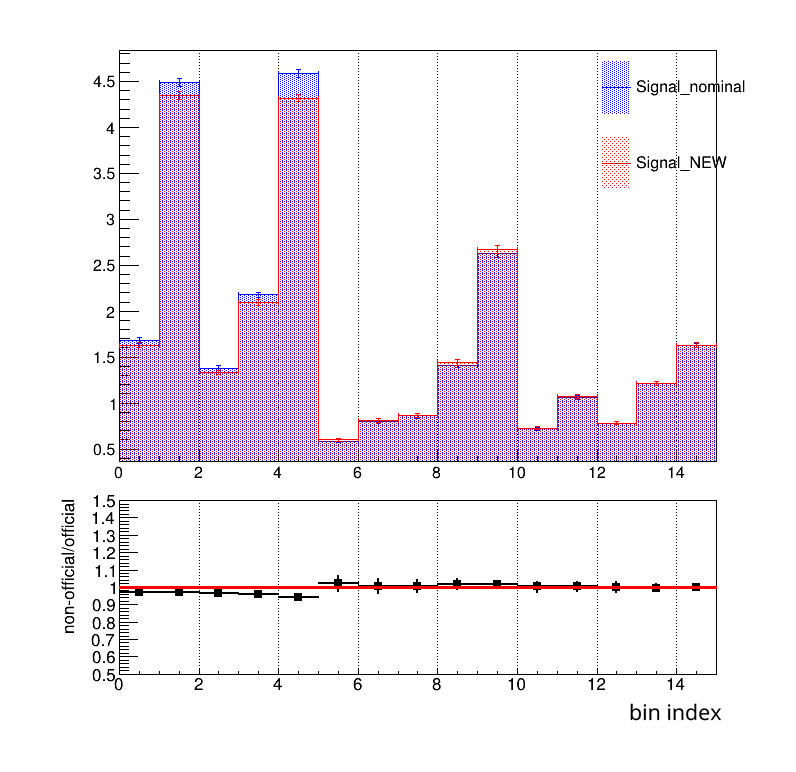
\includegraphics[width=0.5\textwidth]{./picture/systematic/FEI_cal_comparison.png}}
  \caption{Comparison of the nominal and alternative signal templates. The blue histogram is obtained using the official FEI calibration factors. For the red histogram, the alternative calibration factors are applied to correctly reconstructed $B_{\textrm{tag}}$ candidates with $\texttt{isSignal}(B_{\textrm{tag}})=1$, while the official factors are retained for all other candidates.}
  \label{fig:FEICAL_comparison}
\end{figure}

In this analysis, the systematic uncertainty is evaluated by varying the FEI calibration factors applied to signal MC events satisfying $\texttt{isSignal}(B_{\textrm{tag}})=1$.
For each toy sample, the alternative FEI calibration factor for each $B_{\textrm{tag}}$ category is first varied according to a Gaussian distribution defined by its central value and statistical uncertainty in Eqs.~\ref{eq:NEWFEI_cal_charged} and~\ref{eq:NEWFEI_cal_neutral}.
The FEI calibration factor used in the toy sample is then varied around the official calibration factor.
The width of this variation is given by the difference between the official factor and the fluctuated alternative factor.
A common standard-Gaussian random variable is used for all $B_{\textrm{tag}}$ categories within each toy sample, while the alternative calibration factors are varied independently according to their statistical uncertainties.

A total of 500 toy samples are generated using this procedure.
For each toy sample, the predicted yields in the fit bins and event categories are recalculated, and the covariance matrix of the predicted yields is constructed.
PCA is applied to this covariance matrix to reduce the number of nuisance parameters while preserving the correlations among the predicted yields.
The leading three eigenvectors and their corresponding eigenvalues are retained as independent nuisance parameters in the fit.
The cumulative explained variance ratio for these three eigenvectors is 1.00.
Figure~\ref{fig:NEWFEICAL_corr} shows the correlation matrices associated with this secondary FEI calibration uncertainty.
\begin{figure}
  \centering
  \subfloat[][Correlation matrix among the fit bins and event categories
  induced by the secondary FEI calibration uncertainty.]
  {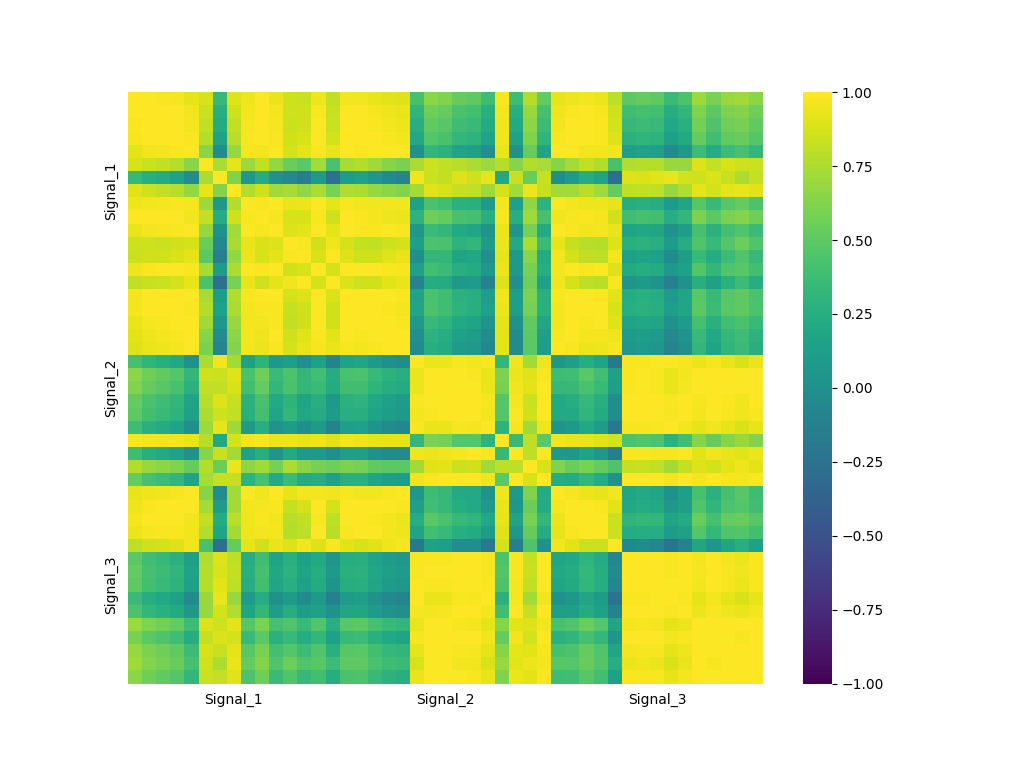
\includegraphics[width=0.45\textwidth]{./picture/systematic/NEWFEICAL_corr_all.png}}
  \hfill
  \subfloat[][Correlation matrix reconstructed using the leading three
  eigenvectors.]
  {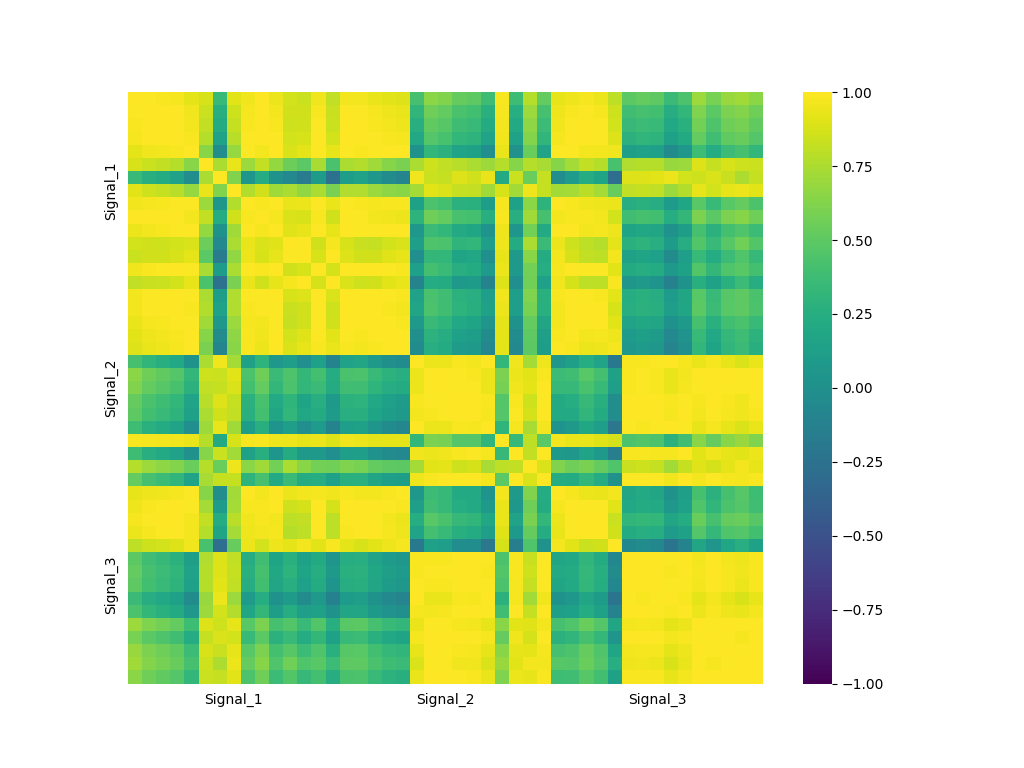
\includegraphics[width=0.45\textwidth]{./picture/systematic/NEWFEICAL_corr_partial.png}}
  \caption{
  Correlation matrices associated with the secondary uncertainty in the
  FEI efficiency correction.
  The left plot is obtained using all eigenvectors, while the right plot is
  reconstructed using the leading three eigenvectors.
  }
  \label{fig:NEWFEICAL_corr}
\end{figure}

\section{$q\bar{q}$ efficiency}
The $q\bar{q}$ background efficiency is corrected using correction factors derived from the off-resonance sample described in Section~\ref{sec:off_resonance}.
The uncertainties in the data-to-MC ratios given in Eq.~\ref{eq:off_resonance_ratio} are assigned as systematic uncertainties.

\section{Photon multiplicity}
As discussed in Section~\ref{sec:photon_mul_corr}, the neutral-tag wrong-charge sideband is used to estimate the uncertainty associated with the photon multiplicity correction.

Figure~\ref{fig:neutral_tag_wrong_charge_sideband} shows the data-to-MC ratios as a function of the number of remaining photon candidates.
These data-to-MC ratios are used to define systematic variations of the photon multiplicity correction factors.

As a validation of this systematic uncertainty, its effect is examined in the $M_{\textrm{bc}}$ sideband.
Figure~\ref{fig:sideband_multiplicity} shows the distribution of the number of remaining photon candidates.
Applying the $+1\sigma$ systematic variation improves the data--MC agreement.
\begin{figure}
  \centering
  \subfloat{
    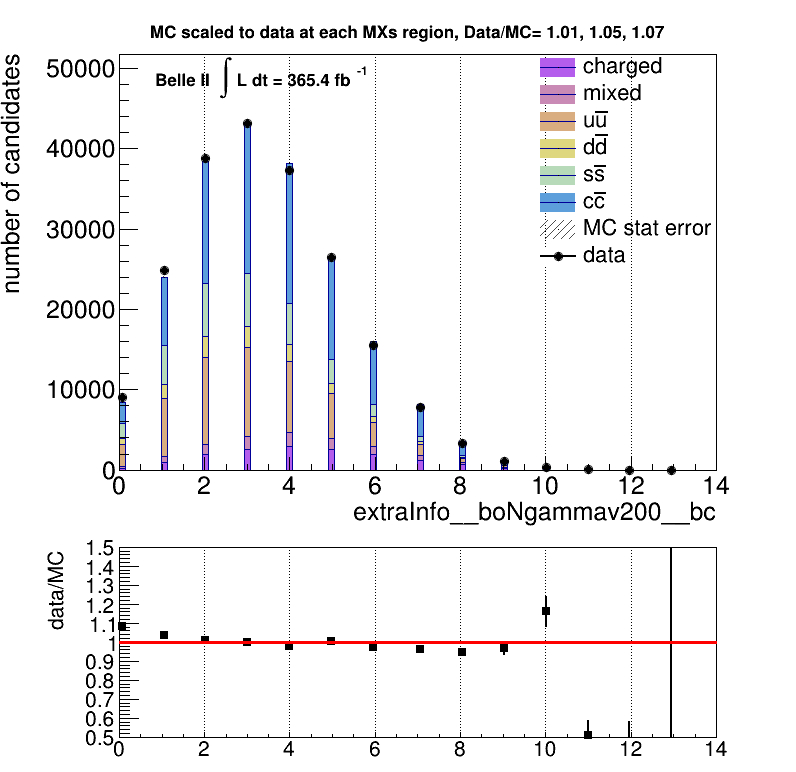
\includegraphics[width=0.45\textwidth]{./picture/sideband/extraInfo__boNgammav200__bc_sideband.png}
  }
  \hfill
  \subfloat{
    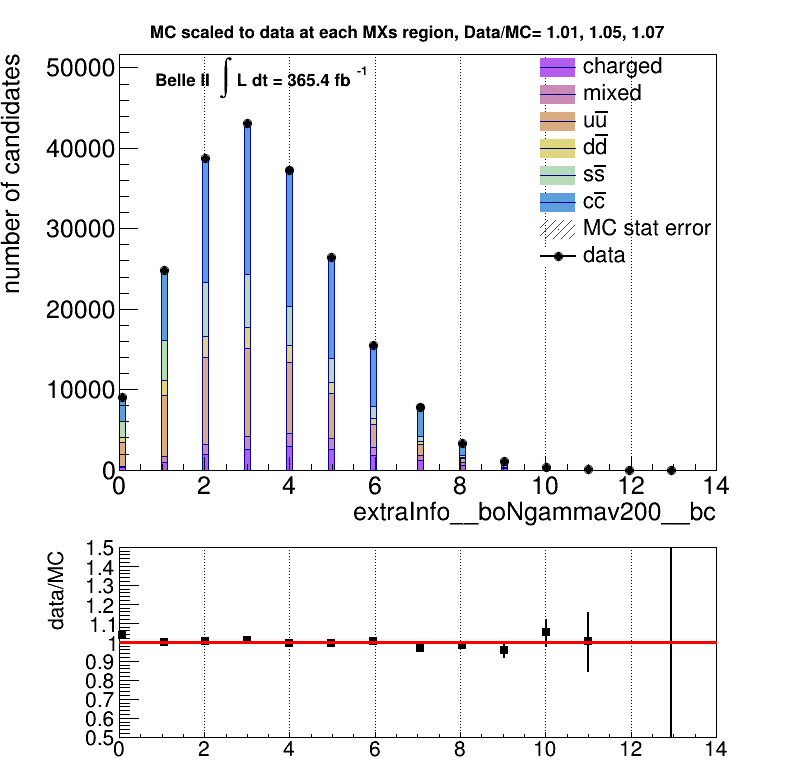
\includegraphics[width=0.45\textwidth]{./picture/sideband_1sigma_multiplicity/extraInfo__boNgammav200__bc_sideband.png}
  }
  \caption{
  Distribution of the number of remaining photon candidates in the
  $M_{\textrm{bc}}$ sideband.
  The left plot shows the distribution obtained with the nominal photon
  multiplicity correction, while the right plot shows the distribution
  obtained with the $+1\sigma$ systematic variation.
  The data--MC agreement is improved by the variation.
  }
  \label{fig:sideband_multiplicity}
\end{figure}

The same procedure described in Section~\ref{sec:hadron_pid_syst} is used to reduce the number of nuisance parameters.

A total of 500 toy samples are generated to estimate the covariance matrix associated with the uncertainties in the photon multiplicity correction factors.
For each toy sample, the photon multiplicity correction factors are varied according to Gaussian distributions defined by their uncertainties.

Figure~\ref{fig:multiplicity_corr} shows the correlation matrices obtained using all eigenvectors and using only the leading two eigenvectors.
The cumulative explained variance ratio for these two eigenvectors is 1.00.
The leading two eigenvectors are retained and implemented as independent nuisance parameters in the fit.
\begin{figure}
  \centering
  \subfloat[][Correlation matrix among the fit bins and event categories
  induced by the uncertainties in the photon multiplicity correction
  factors.]
  {
    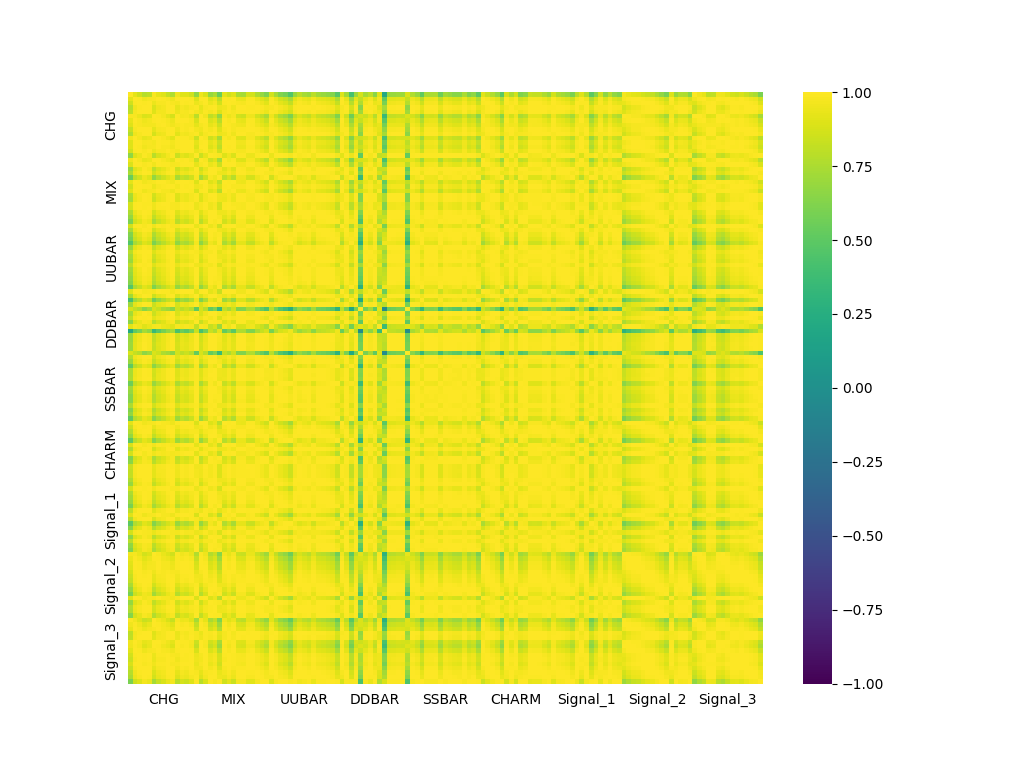
\includegraphics[width=0.45\textwidth]{./picture/systematic/multiplicity_corr_all.png}
  }
  \hfill
  \subfloat[][Correlation matrix reconstructed using the leading two
  eigenvectors.]
  {
    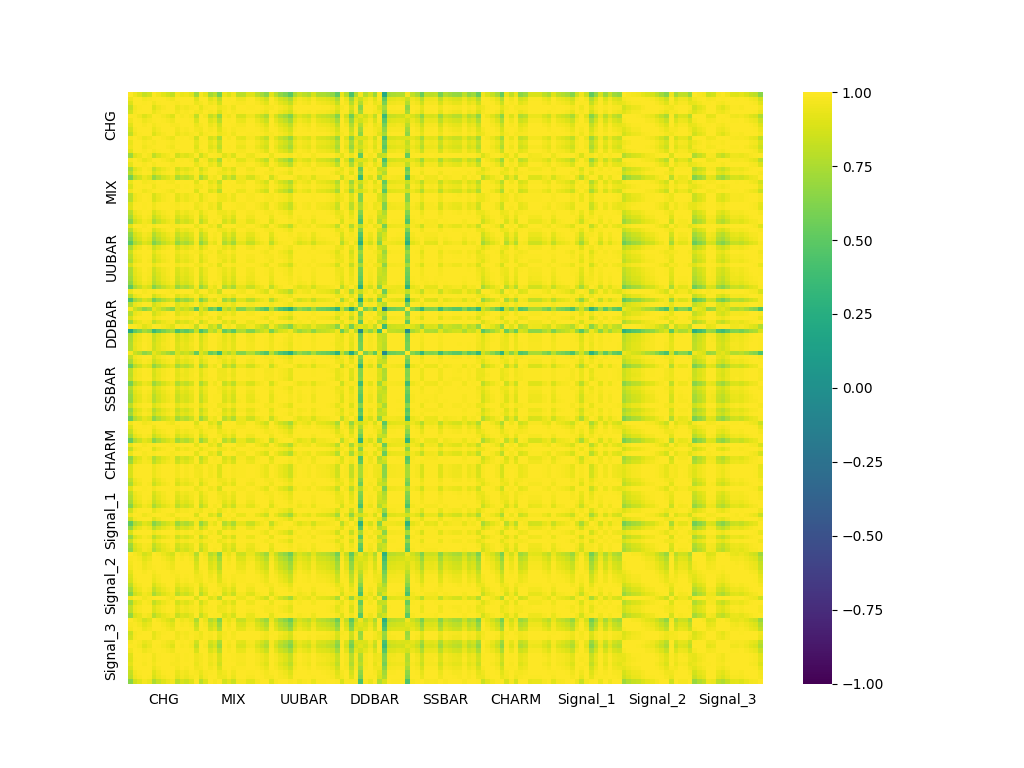
\includegraphics[width=0.45\textwidth]{./picture/systematic/multiplicity_corr_partial.png}
  }
  \caption{
  Correlation matrices associated with the systematic uncertainty in the photon multiplicity correction factors.
  The left plot is obtained using all eigenvectors, while the right plot is reconstructed using the leading two eigenvectors.
  }
  \label{fig:multiplicity_corr}
\end{figure}

\section{Fraction of decay modes}
Because the branching ratios of $B\rightarrow K\nu\bar{\nu}$, $B\rightarrow K^{*}\nu\bar{\nu}$, and the remaining $B\rightarrow X_{s}\nu\bar{\nu}$ have uncertainties, the relative fractions of these decay modes are also uncertain.
The branching ratios are~\cite{Buras:2014fpa,Parrott:2022zte}
\begin{align}
  BR(\textrm{B}^{+}\rightarrow K^{+}\nu \bar{\nu})_{SM}&=(5.044 \pm 0.402) \times 10^{-6},\\
  BR(\textrm{B}^{0}\rightarrow K^{*0}\nu \bar{\nu})_{SM}&=(9.19 \pm 0.86 \pm 0.50) \times 10^{-6}.
\end{align}
The first uncertainty in $BR(B^{0}\rightarrow K^{*0}\nu\bar{\nu})_{\mathrm{SM}}$ arises from the form factors.
Because the form-factor uncertainty is already included in Section~\ref{subsec:formfactor_uncertainty}, only the second uncertainty is considered here.

In addition, the uncertainties in the $B\rightarrow K$ form factors result in a relative uncertainty of $^{+0.056}_{-0.055}$ in the $B\rightarrow K\nu\bar{\nu}$ branching ratio.
This relative uncertainty is calculated using the correlation matrix given in Ref.~\cite{Parrott:2022rgu}.
After excluding the form-factor contribution, the remaining relative uncertainty is $\pm 0.057$.

Using these uncertainties, the uncertainties in the relative fractions of the $B\rightarrow K\nu\bar{\nu}$, $B\rightarrow K^{*}\nu\bar{\nu}$, and the remaining $B\rightarrow X_{s}\nu\bar{\nu}$ decay modes are evaluated.

\section{Fermi motion momentum}
The Fermi motion momentum $p_{F}$ in Eq.~\ref{eq:pf} is used to produce the signal MC samples.
To estimate the uncertainty associated with the Fermi motion momentum, signal samples with different $p_{F}$ values are produced without detector simulation.

Figure~\ref{fig:pf_syst} shows the $M_{X_{s}}$ distributions obtained with different $p_{F}$ values.
The discontinuities arise from the fragmentation correction described in Section~\ref{sec:frag_corr}.
The weights are obtained from the ratios of the $M_{X_{s}}$ distributions
generated with varied and nominal $p_{F}$ values.
These weights are applied to the nominal signal MC sample, and the resulting changes in the signal templates are assigned as the systematic uncertainty associated with the Fermi motion momentum.
\begin{figure}
  \centering
  \subfloat[][$M_{X_{s}}$ distributions for the charged signal sample obtained with different $p_{F}$
  values. The discontinuities arise from the fragmentation correction
  described in Section~\ref{sec:frag_corr}.]{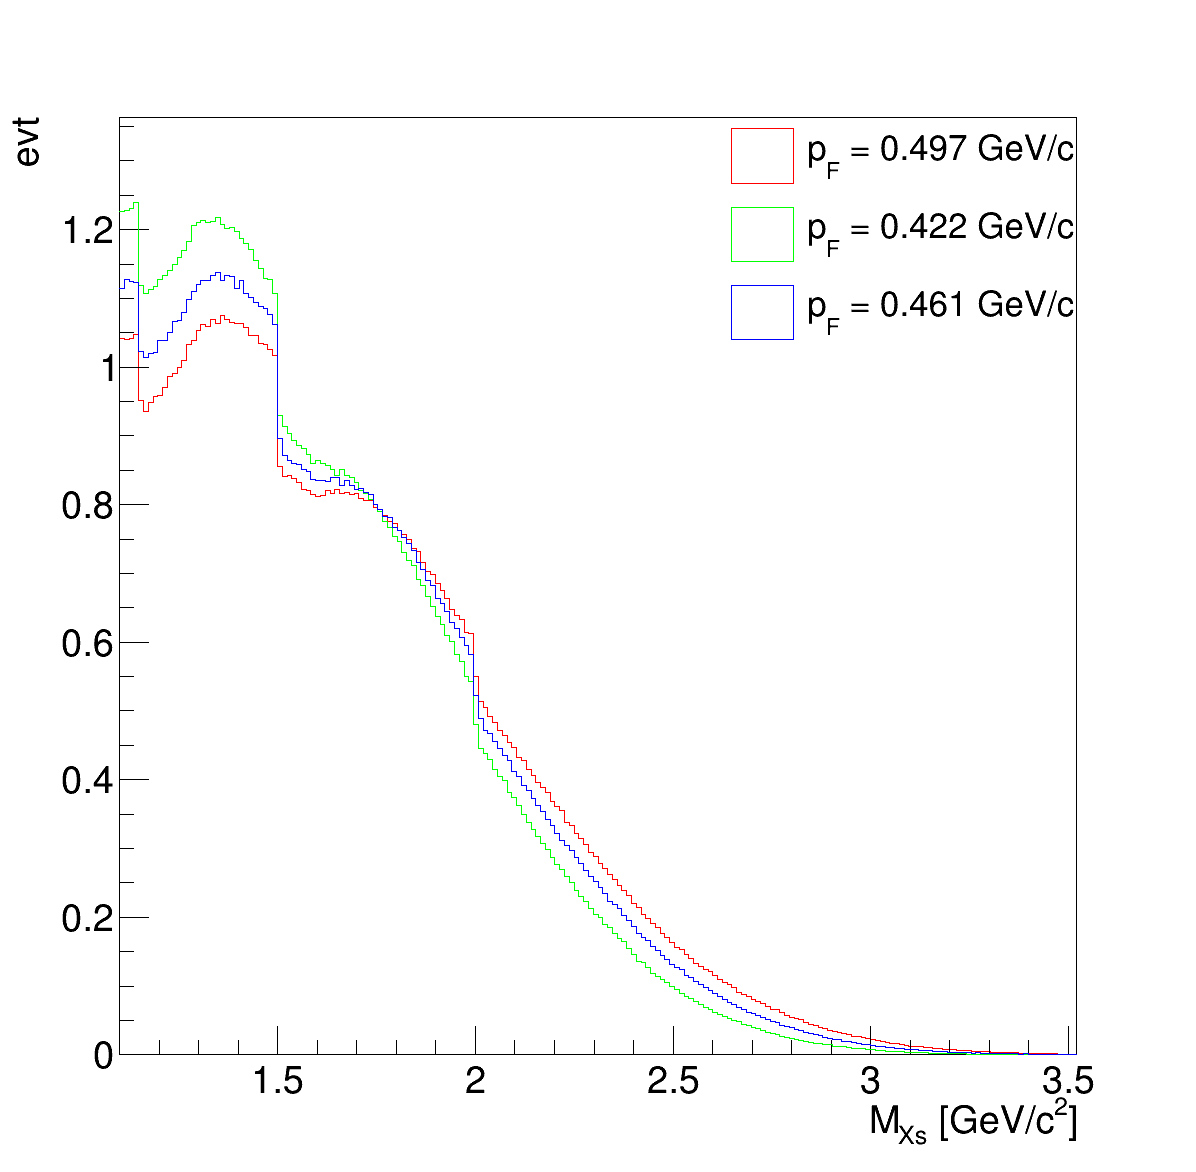
\includegraphics[width=0.45\textwidth]{./picture/systematic/Xsu_pf.png}}
  \hfill
  \subfloat[][$M_{X_{s}}$ distributions for the neutral signal sample obtained with different $p_{F}$
  values. The discontinuities arise from the fragmentation correction
  described in Section~\ref{sec:frag_corr}.]{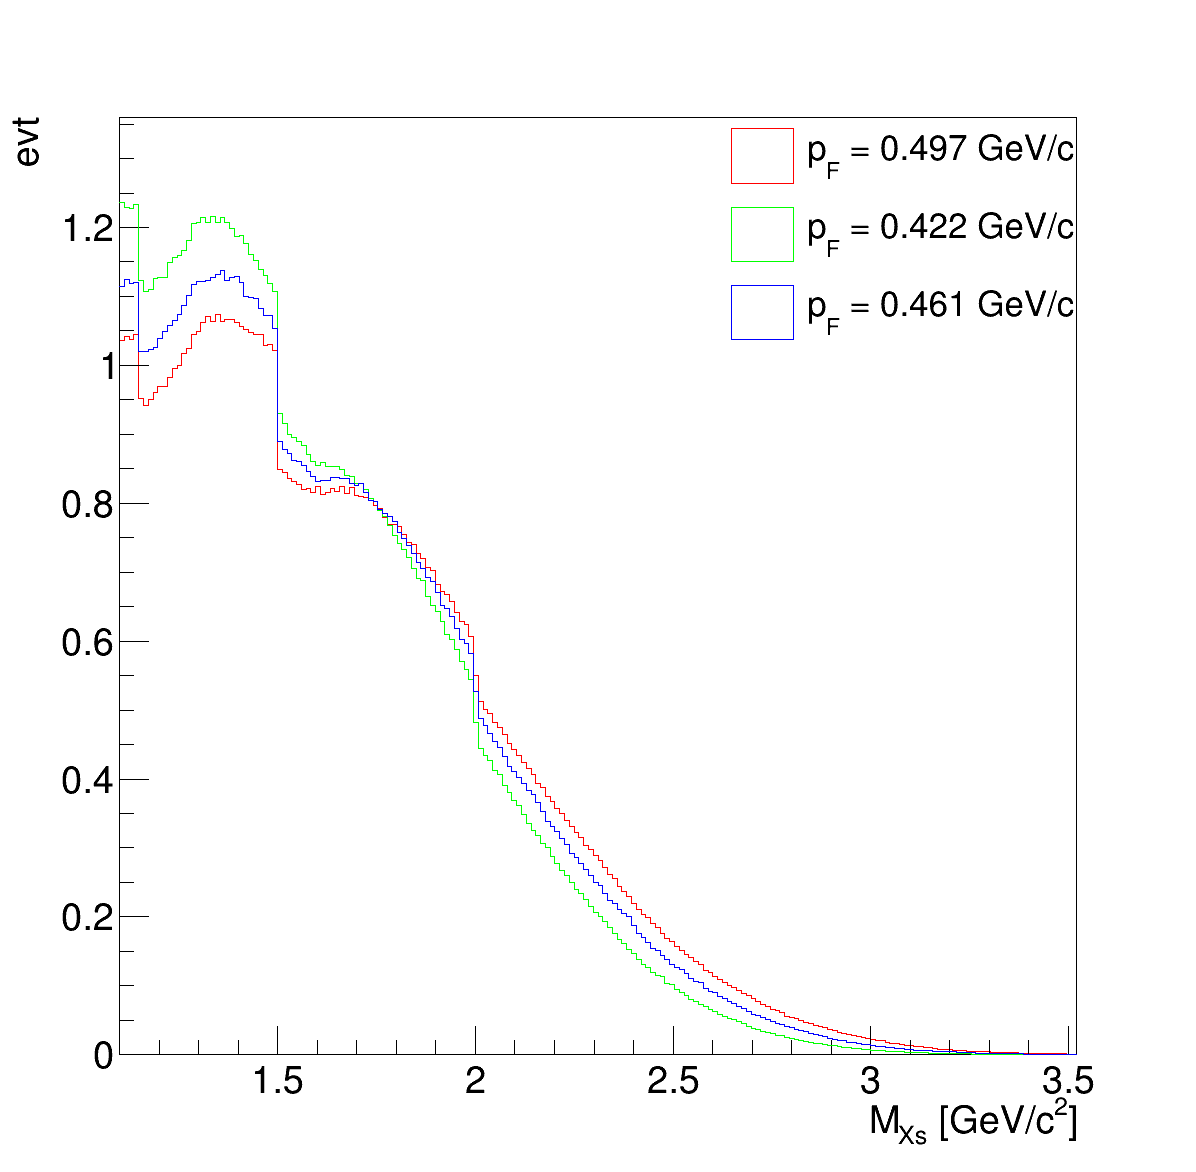
\includegraphics[width=0.45\textwidth]{./picture/systematic/Xsd_pf.png}}
  \caption{}
  \label{fig:pf_syst}
\end{figure}

\section{$K^{*}-X_{s}$ transition}
As discussed in Section~\ref{subsec:signal_MC}, the remaining $B \rightarrow X_{s} \nu \bar{\nu}$ sample, excluding $B\rightarrow K \nu \bar{\nu}$ and $B \rightarrow K^{*} \nu \bar{\nu}$, is generated with the requirement $M_{X_{s}} > 1.1~\textrm{GeV}/c^{2}$.

To estimate the systematic uncertainty associated with this mass threshold, the remaining $B \rightarrow X_{s} \nu \bar{\nu}$ samples are generated with varied threshold values of $M_{X_{s}} = 1.1 \pm 0.1~\textrm{GeV}/c^{2}$.
The variation of $0.1~\textrm{GeV}/c^{2}$ is motivated by the $M_{X_{s}}$ distribution in the $B \rightarrow X_s\gamma$ study~\cite{Belle:2014nmp}.
The resulting changes in the event yields in the fit bins are assigned as the systematic uncertainty.

Non-$K^{(*)}$ components may contribute below $1.0~\textrm{GeV}/c^{2}$.
To quantify this effect, the impact of the S-wave component in $K\pi\nu\bar{\nu}$ decays is examined.
As discussed in Section~\ref{sec:K700}, the S-wave component does not change the final result at the first decimal place.
Therefore, no additional systematic uncertainty associated with non-$K^{(*)}$ components below $1.0~\textrm{GeV}/c^{2}$ is included.

\section{b-quark mass}
The mass of the $b$ quark is used as a parameter in the decay amplitude given in Eq.~\ref{eq:Xsamp}.
The value of this parameter varies among theoretical calculations~\cite{Altmannshofer:2009ma,Ali:1999mm}.
Conservatively, the following value is used in this analysis:
\begin{equation}
  m_{b} = 4.68 \pm 0.15~\textrm{GeV}/c^{2}.
\end{equation}

To estimate the systematic uncertainty associated with the $b$-quark mass, signal samples with varied $b$-quark mass values are generated without detector simulation.
Figure~\ref{fig:mb_syst} shows the $q^{2}$ distributions obtained with different $m_{b}$ values.
Weights are derived from the ratios of the $q^{2}$ distributions generated with varied and nominal $m_{b}$ values.
These weights are applied to the nominal signal MC sample, and the resulting changes in the signal templates are assigned as the systematic uncertainty associated with the $b$-quark mass.
\begin{figure}
  \centering
  \subfloat[][$q^{2}$ distributions for the charged signal sample obtained with different $m_{b}$ values.]
  {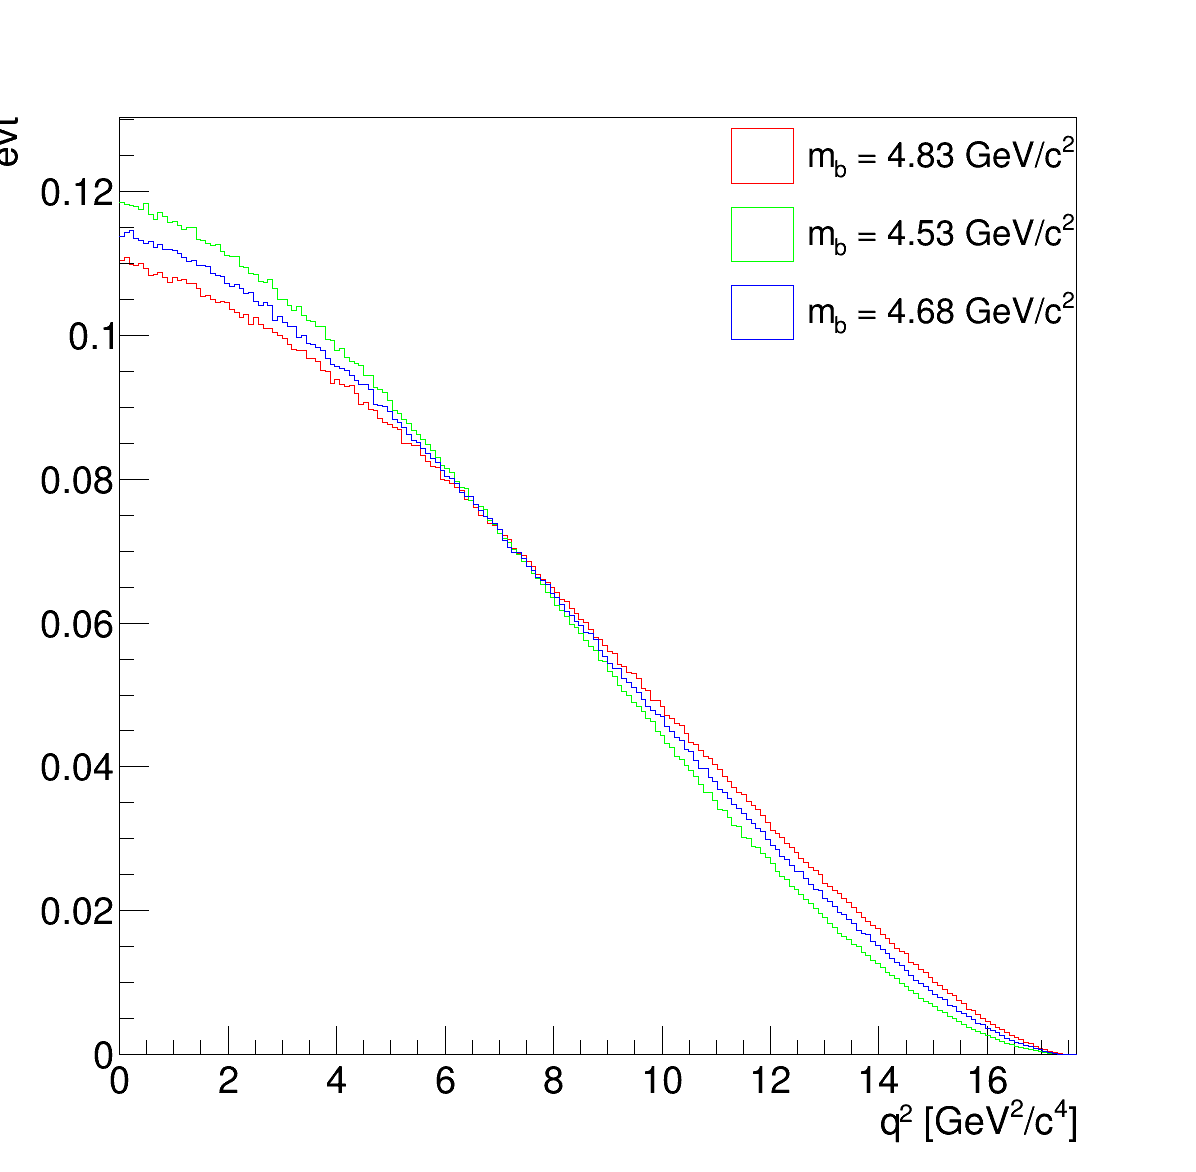
\includegraphics[width=0.45\textwidth]{./picture/systematic/Xsu_mb.png}}
  \hfill
  \subfloat[][$q^{2}$ distributions for the neutral signal sample obtained with different $m_{b}$ values.]
  {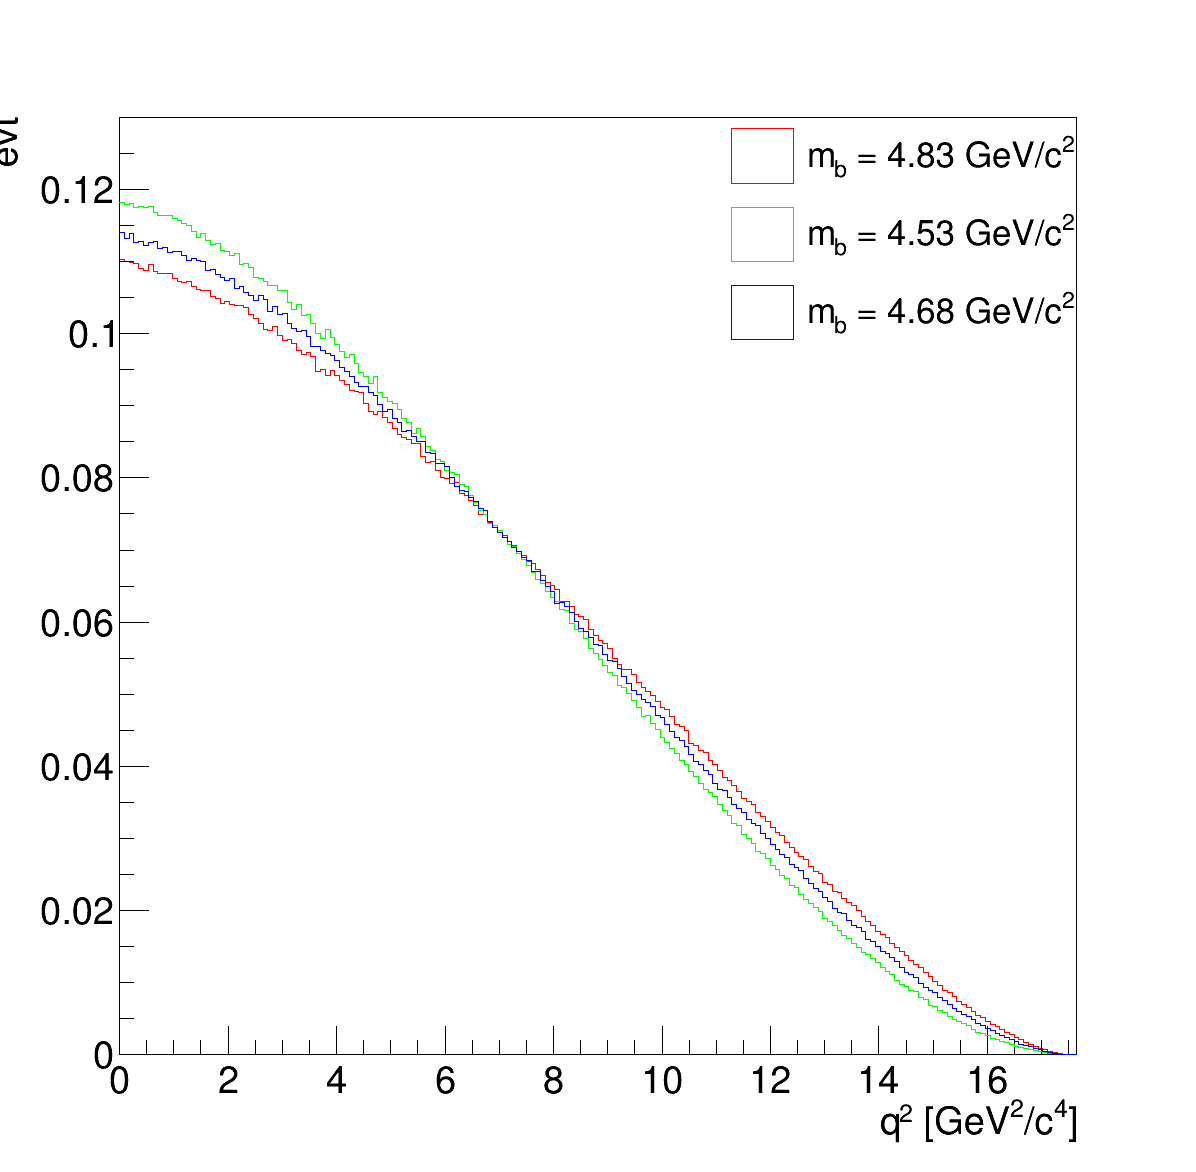
\includegraphics[width=0.45\textwidth]{./picture/systematic/Xsd_mb.png}}
  \caption{
  $q^{2}$ distributions for the charged and neutral signal samples generated with different $b$-quark mass values.
  }
  \label{fig:mb_syst}
\end{figure}

\section{MC statistics}
Because of the finite sizes of the MC samples, the histogram templates have statistical uncertainties.
These uncertainties are included as systematic uncertainties.

\section{Fragmentation of $X_{s}$}
As discussed in Section~\ref{sec:frag_corr}, the correction for the fragmentation of $X_{s}$ is derived using $B \rightarrow X_{s} \gamma$ decays.
The systematic uncertainty associated with the fragmentation correction is estimated using two methods.
The first method uses the difference between the fragmentations observed in $B \rightarrow X_{s} \gamma$ and $B \rightarrow X_{s} J/\psi$ decays.
The second method is based on fluctuations of \texttt{PYTHIA} parameters.
Both methods are used because the previous $B \rightarrow X_{s} J/\psi$ study does not cover all $X_{s}$ decay modes and $M_{X_{s}}$ regions.

Figure~\ref{fig:fragmentation_compare} compares the fragmentations in $B \rightarrow X_{s} \gamma$~\cite{Belle:2018iff,Belle:Xsgamma} and $B \rightarrow X_{s} J/\psi$ decays~\cite{Belle:2014owz,Belle:Xsll_Yutaro}.
Here, the fragmentation in $B \rightarrow X_{s} J/\psi$ decays is obtained from the MC sample after applying the overall correction factor.
This correction factor is an overall factor and does not depend on $M_{X_{s}}$.
In general, the fragmentations in $B \rightarrow X_{s} \gamma$ and $B \rightarrow X_{s} J/\psi$ decays are in good agreement.
However, some differences are observed for several modes, such as the $K2\pi$ mode with one $\pi^{0}$.
In the regions $1.15<M_{X_{s}}<1.5~\textrm{GeV}/c^{2}$ and $1.5<M_{X_{s}}<2.0~\textrm{GeV}/c^{2}$, the differences for the seven decay modes shown in Figure~\ref{fig:fragmentation_compare} are assigned as systematic uncertainties.
\begin{figure}
  \centering
  \subfloat[][$1.15<M_{X_{s}}<1.5~\textrm{GeV}/c^{2}$]{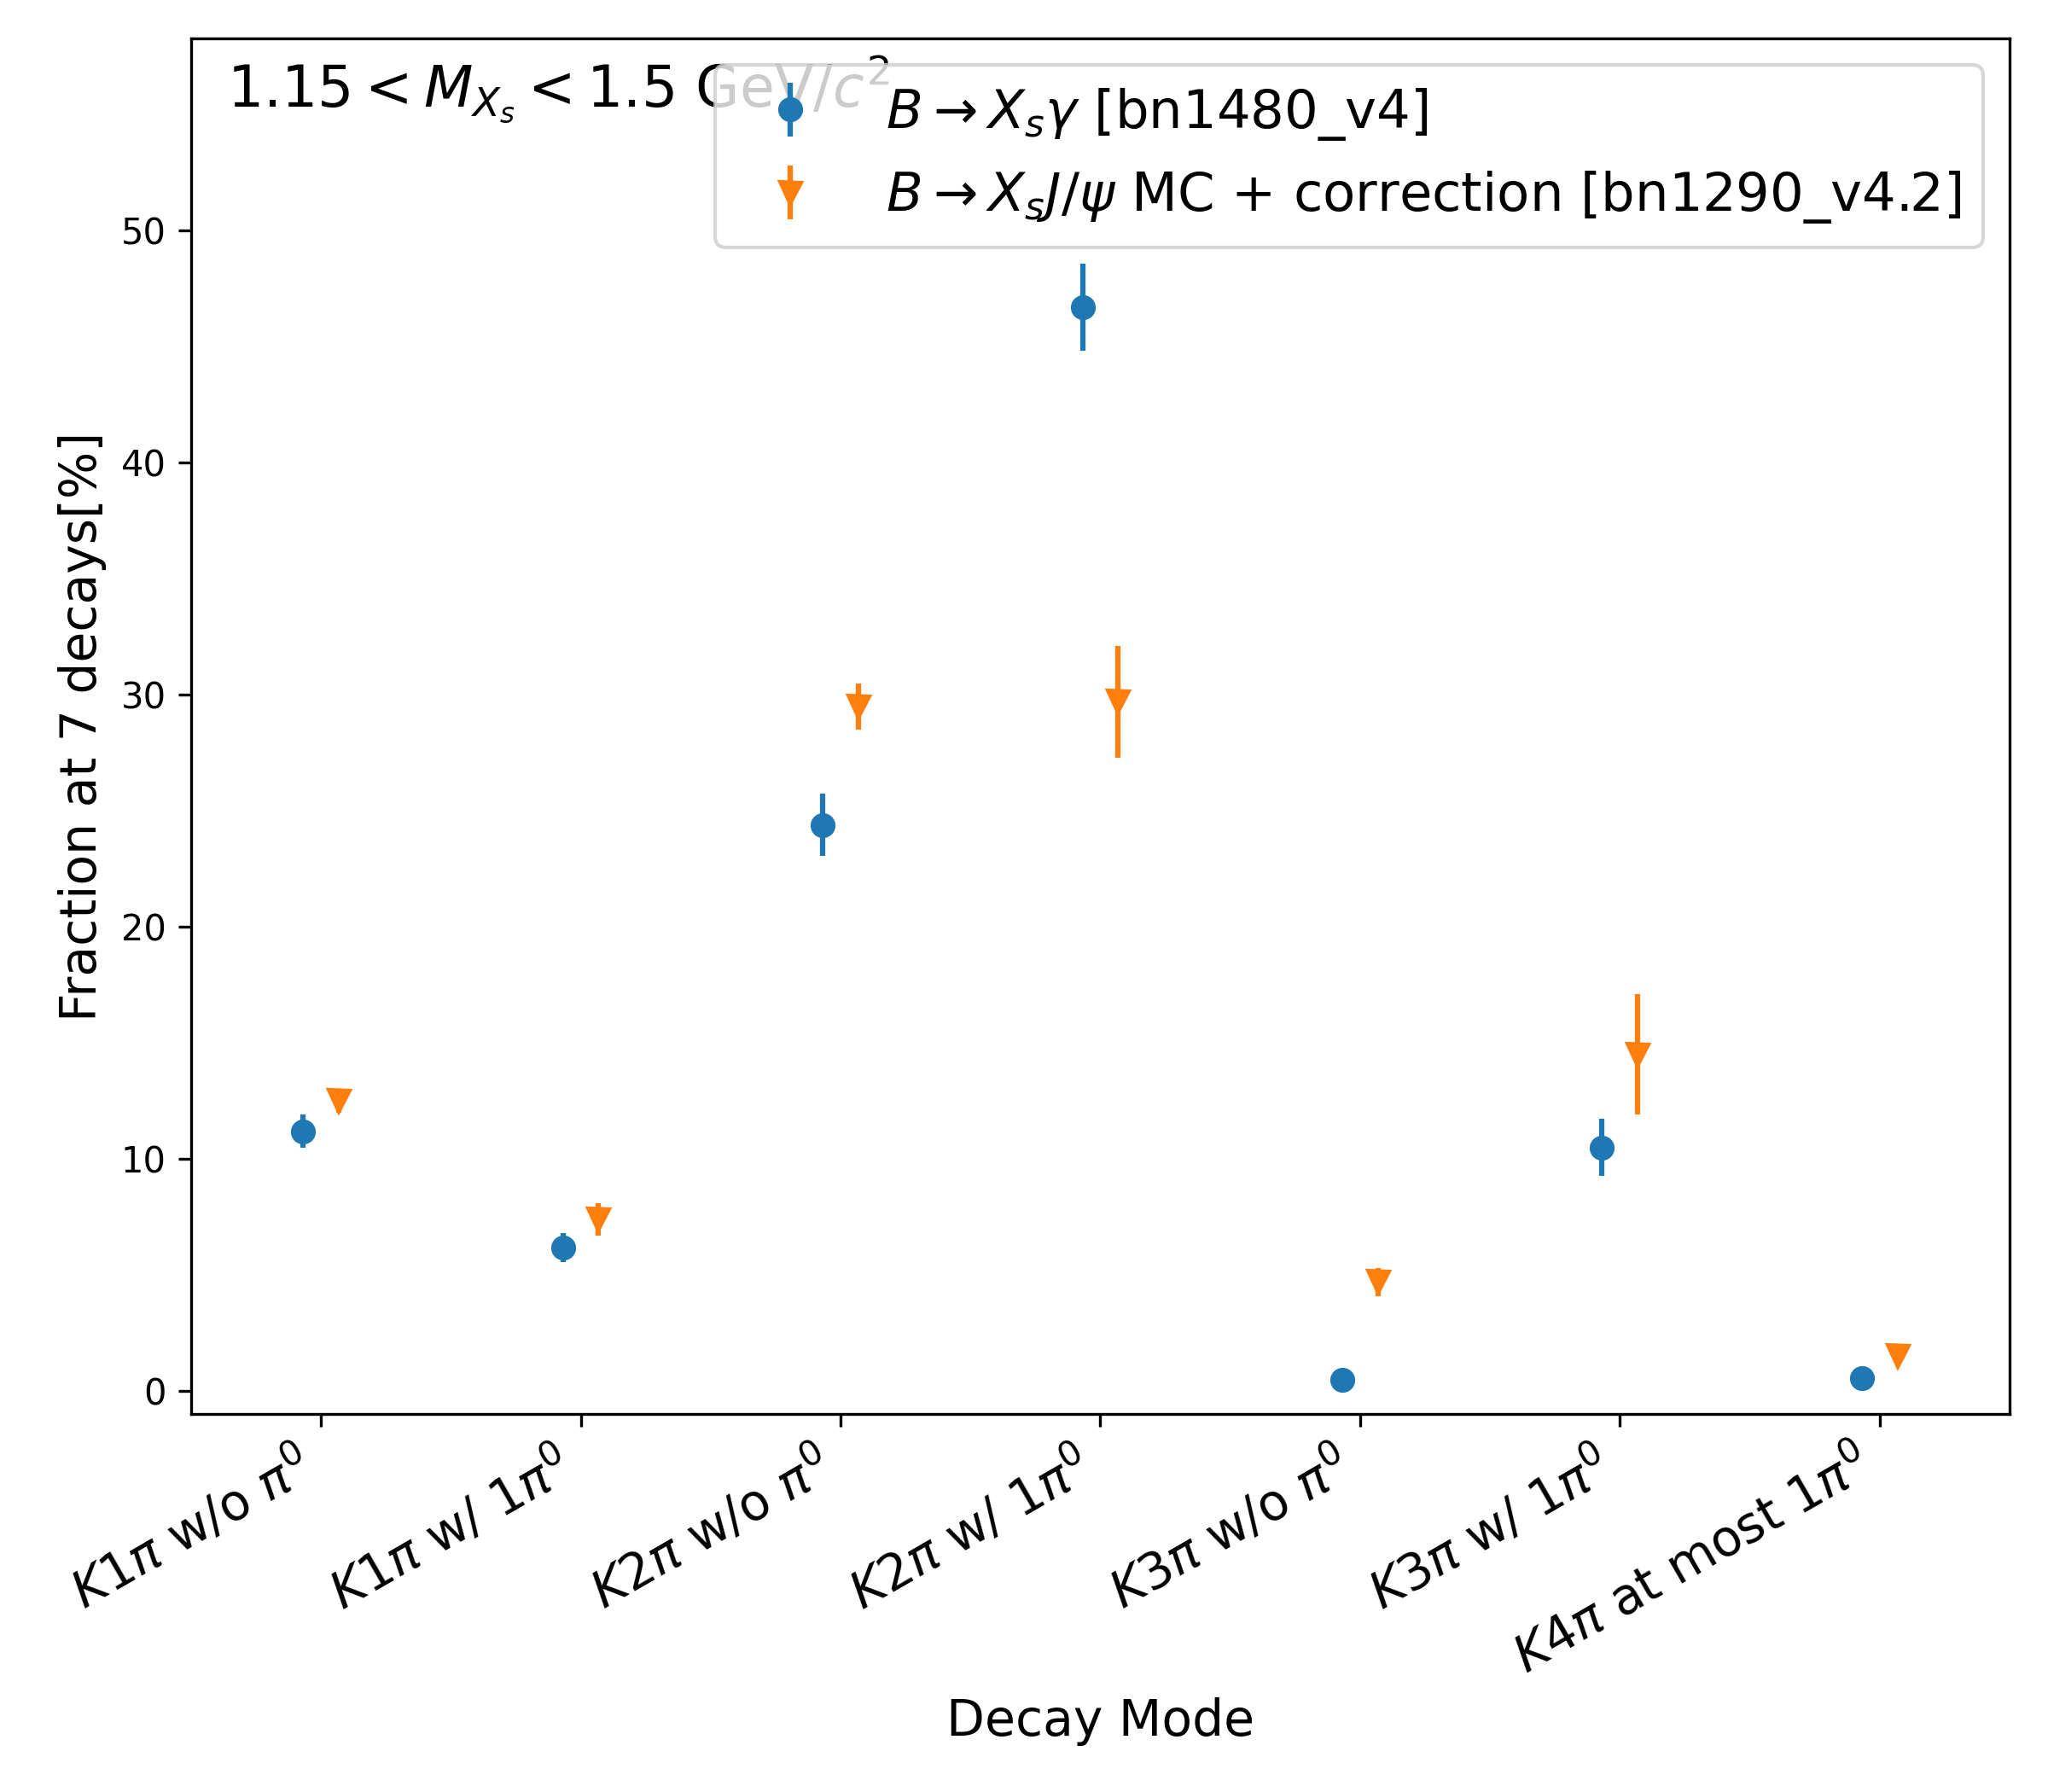
\includegraphics[width=0.45\textwidth]{./picture/systematic/fragmentation_compare_1.15_1.5.png}}
  \hfill
  \subfloat[][$1.5<M_{X_{s}}<2.0~\textrm{GeV}/c^{2}$]{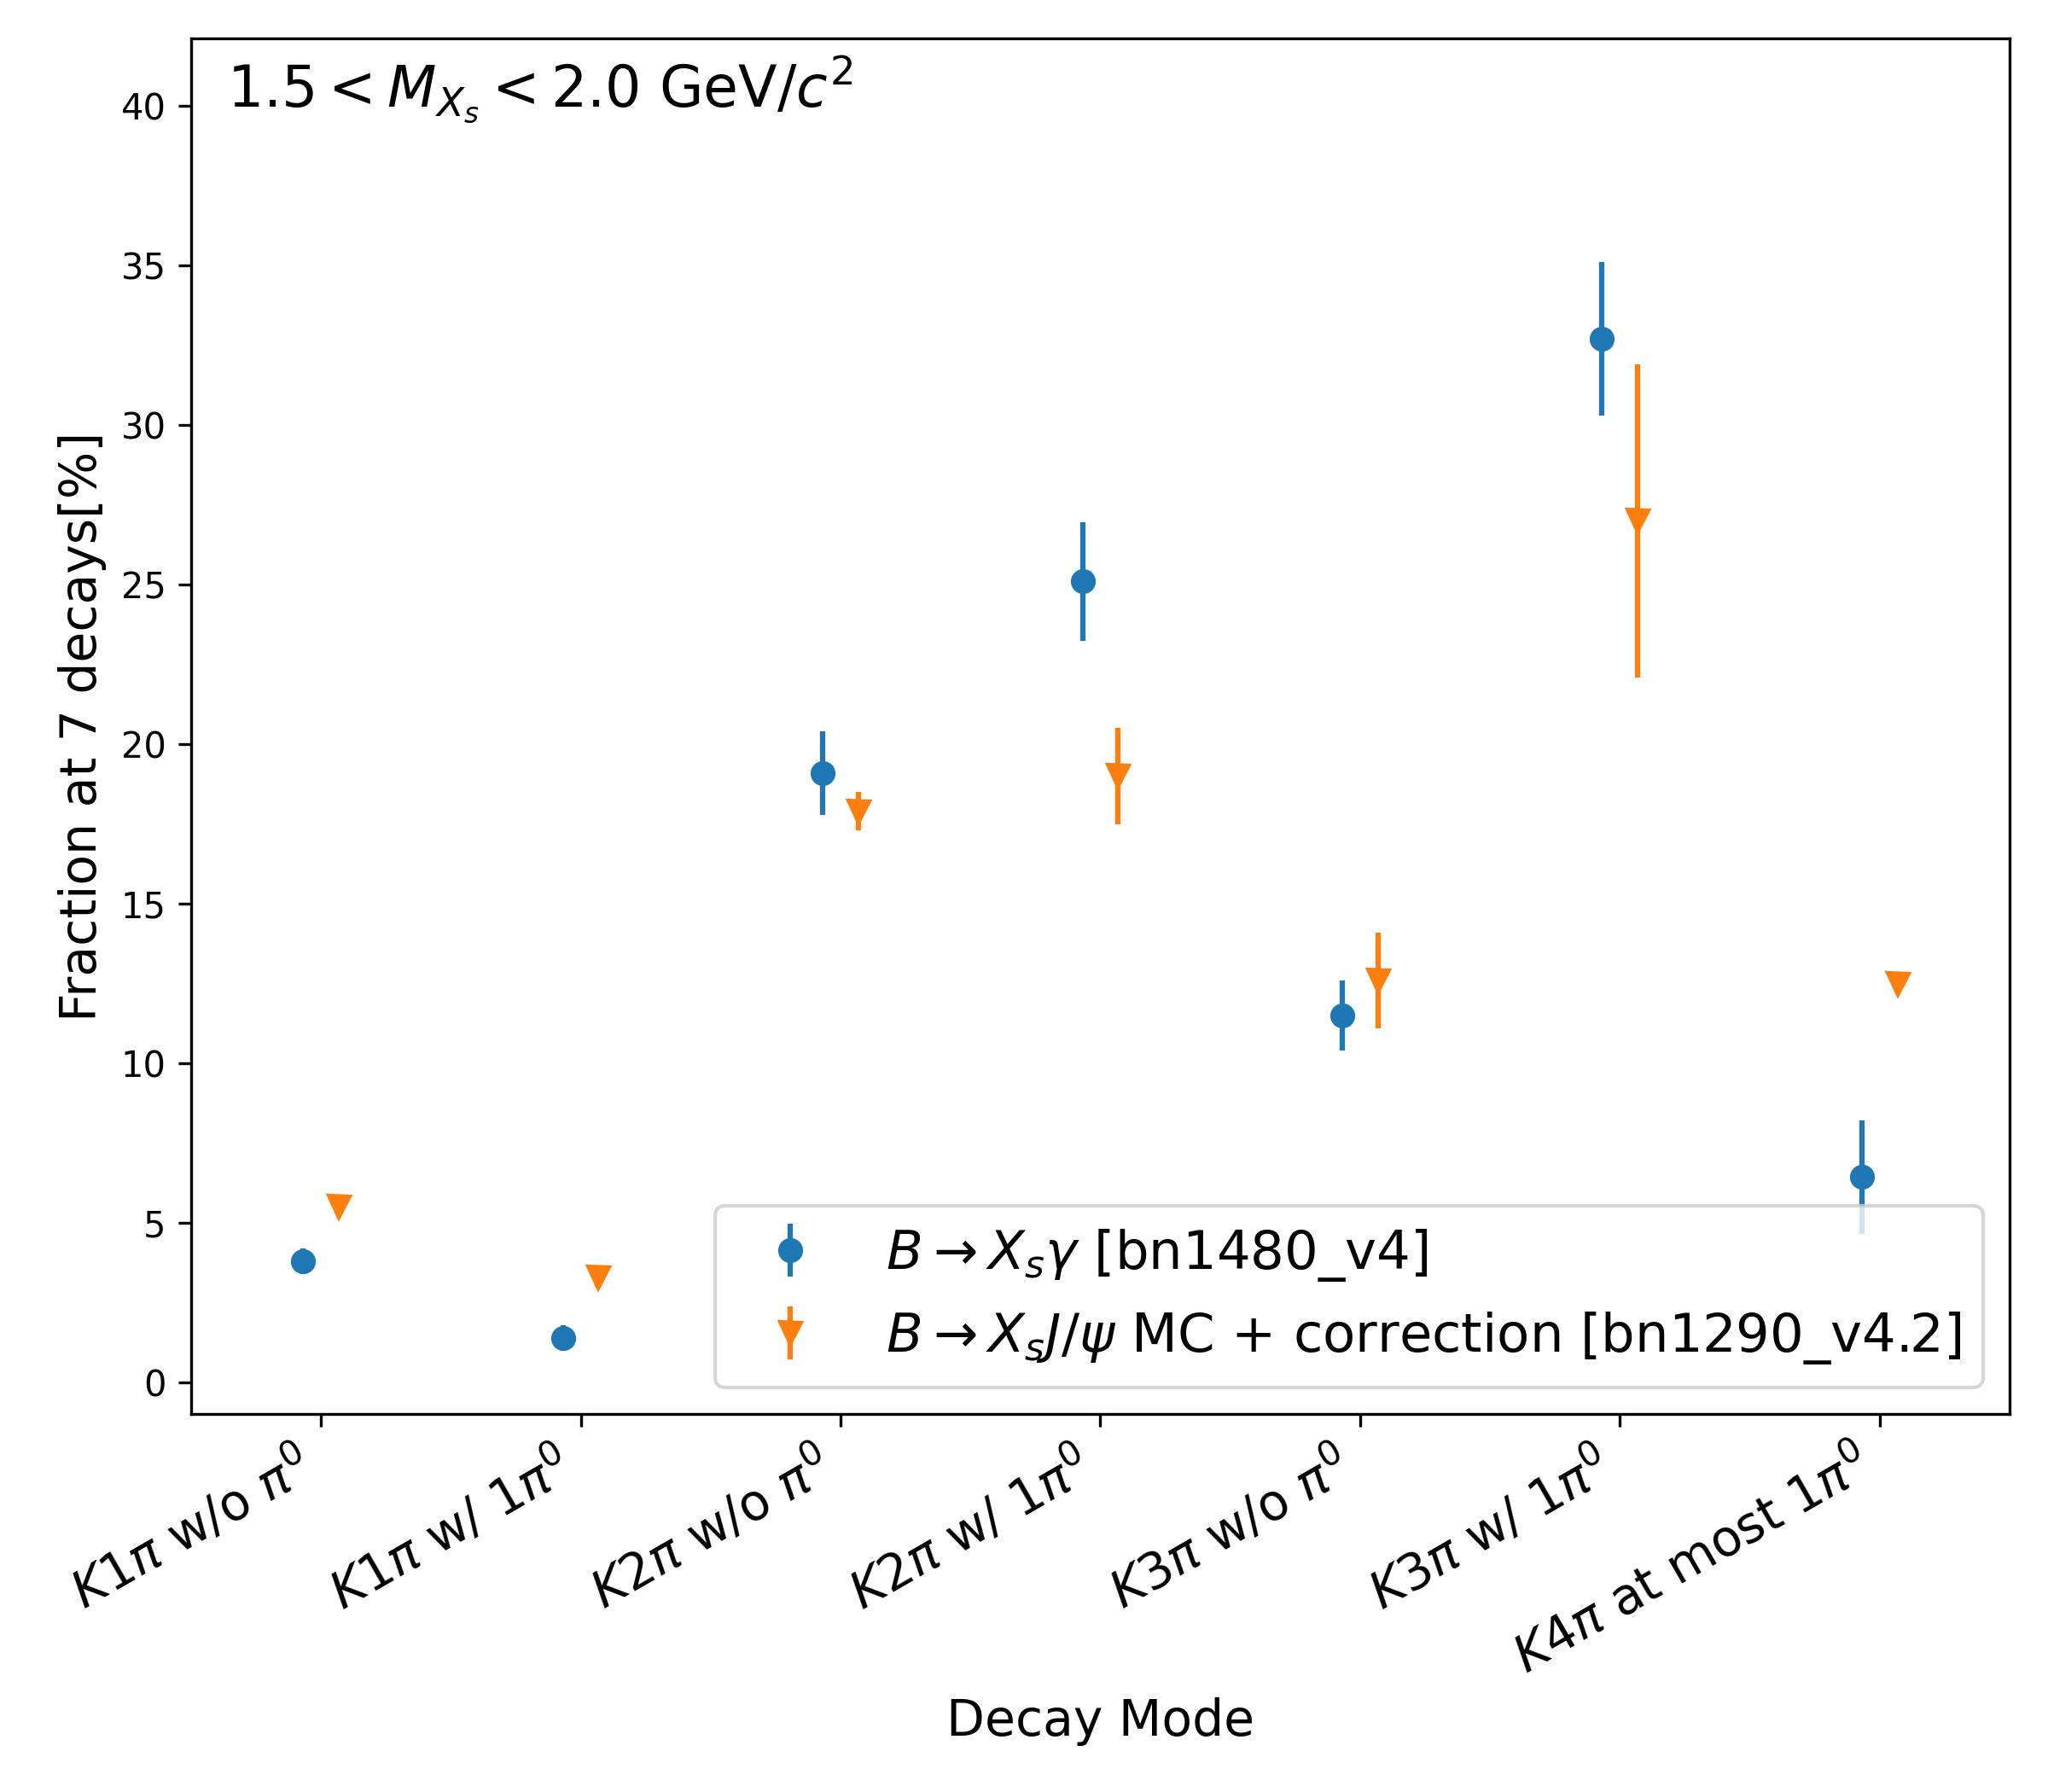
\includegraphics[width=0.45\textwidth]{./picture/systematic/fragmentation_compare_1.5_2.0.png}}
  \caption{Comparison of the fragmentations in $B \rightarrow X_{s} \gamma$ and $B \rightarrow X_{s} J/\psi$ decays.}
  \label{fig:fragmentation_compare}
\end{figure}

For the remaining decay categories and $M_{X_{s}}$ regions, the systematic uncertainty in the fragmentation is estimated by fluctuating \texttt{PYTHIA} parameters.
This method has been used in other $B \rightarrow X_{s} \gamma$ studies~\cite{Belle:2018iff,Belle:2014nmp}.
Table~\ref{tab:Pythia_fluctuation} summarizes the varied \texttt{PYTHIA} parameters and their tested values.
\begin{table}
\caption{
        Summary of the fluctuated \texttt{PYTHIA} parameters.
        Among the tested values, combinations are selected such that the fragmentations of the seven decay categories shown in Figure~\ref{fig:fragmentation_compare} are within $2\sigma$ of the $B\rightarrow X_s\gamma$ result.
        Here, $\sigma$ is defined as the difference between the
        $B \rightarrow X_s\gamma$ and $B\rightarrow X_s J/\psi$ studies.
    }
    \renewcommand{\arraystretch}{1.4}
    \setlength{\tabcolsep}{4pt}
    \centering
    \small

    \begin{tabularx}{\textwidth}{
        >{\raggedright\arraybackslash}p{5.0cm}
        >{\raggedright\arraybackslash}X
        >{\centering\arraybackslash}p{2.6cm}
    }
        \hline
        \hline
        Parameter name & Description & Tested values \\
        \hline

        \mbox{\texttt{StringFlav:probStoUD}}
        &
        The suppression of $s$ quark pair production in the field compared with $u$ or $d$ pair production
        &
        $[0.0, 0.3, 0.6]$ \\

        \mbox{\texttt{StringFlav:etaSup}}
        &
        Extra suppression factor for $\eta$ production \newline in fragmentation
        &
        $[0.4, 0.7, 1.0]$ \\

        \mbox{\texttt{StringFlav:mesonUDvector}}
        &
        The relative production ratio vector/pseudoscalar for light mesons
        &
        $[2.0, 2.5, 3.0]$ \\

        \mbox{\texttt{StringFlav:mesonSvector}}
        &
        The relative production ratio vector/pseudoscalar for strange mesons
        &
        $[2.0, 2.5, 3.0]$ \\

        \mbox{\texttt{StringFlav:mesonSL1S1J0}}
        &
        The relative scalar production ratio \newline (L=1,S=1,J=0)/pseudoscalar for strange mesons
        &
        $[2.0, 2.5, 3.0]$ \\

        \mbox{\texttt{StringFlav:mesonSL1S1J2}}
        &
        The relative tensor production ratio \newline (L=1,S=1,J=2)/pseudoscalar for strange mesons
        &
        $[2.3, 2.8, 3.0]$ \\

        \hline
        \hline
    \end{tabularx}

    \label{tab:Pythia_fluctuation}
\end{table}
The tested values are chosen based on the fragmentation in the $B \rightarrow X_{s} \gamma$ study.
Among the parameter combinations listed in Table~\ref{tab:Pythia_fluctuation}, combinations are selected such that the fragmentations of the seven decay categories shown in Figure~\ref{fig:fragmentation_compare} are within $2\sigma$ of the $B\rightarrow X_{s}\gamma$ result.
Here, $\sigma$ is defined as the difference between the $B \rightarrow X_{s} \gamma$ and $B \rightarrow X_{s} J/\psi$ studies.
The systematic uncertainty is assigned as the maximum deviation from the nominal value.
Table~\ref{tab:Pythia_fluctuation_result} shows the nominal fragmentation fractions used in this analysis and the maximally deviated fractions obtained from the \texttt{PYTHIA} parameter fluctuations.
An entry is left empty when the systematic uncertainty is estimated from the difference between the $B \rightarrow X_{s} \gamma$ and $B \rightarrow X_{s} J/\psi$ studies.
\begin{sidewaystable}
\caption{Summary of the results obtained by fluctuating the \texttt{PYTHIA} parameters. The fractions of the nine decay categories are shown for the nominal MC sample and for the maximally deviated \texttt{PYTHIA} parameter combination. The fractions of missing decay modes are also shown. An entry is left empty when the systematic uncertainty is estimated from the difference between the $B \rightarrow X_{s} \gamma$ and $B \rightarrow X_{s} J/\psi$ studies.}
  \renewcommand{\arraystretch}{1.4}
  \centering

\begin{adjustbox}{max width=0.98\textheight}
\begin{tabular}{ p{3.5cm} p{1.2cm} p{1.2cm} p{1.2cm} p{1.2cm} p{1.2cm} p{1.2cm} p{1.2cm} p{1.2cm} p{1.2cm} p{1.2cm}}
 \hline
  \hline
 & \multicolumn{10}{c}{nominal and maximally deviated fraction in each $M_{X_{s}}$ region ($\textrm{GeV}$)} \\\cline{2-11}
 & \multicolumn{2}{c}{[0.0,1.15]} & \multicolumn{2}{c}{[1.15,1.5]} & \multicolumn{2}{c}{[1.5,2.0]} & \multicolumn{2}{c}{[2.0,2.4]} & \multicolumn{2}{c}{[2.4,$\infty$)}\\
decay category &  nom & max & nom & max & nom & max & nom & max & nom & max \\
 \hline
$K1\pi$ w/o $\pi^{0}$ & 39\% & 17\% & 11\% & - & 3.8\% & - & 1.7\% & 2.6\% & 9.9\% & 1.1\% \\
$K1\pi$ w/ 1$\pi^{0}$ & 19\% & 8.4\% & 6.2\% & - & 1.4\% & - & 0.5\% & 1.3\% & 5.0\% & 0.5\% \\
$K2\pi$ w/o $\pi^{0}$ & 17\% & 33\% & 24\% & - & 19\% & - & 9.0\% & 10\% & 11\% & 5.6\% \\
$K2\pi$ w 1$\pi^{0}$ & 17\% & 34\% & 47\% & - & 25\% & - & 8.0\% & 13\% & 13\% & 7.6\% \\
$K3\pi$ w/o $\pi^{0}$ & 0.4\% & 0.1\% & 0.5\% & - & 12\% & - & 17\% & 9.3\% & 6.6\% & 9.8\% \\
$K3\pi$ w 1$\pi^{0}$ & 3.0\% & 0.2\% & 11\% & - & 33\% & - & 27\% & 24\% & 16\% & 22\% \\
$K4\pi$ at most 1$\pi^{0}$ & 0.0\% & 0.0\% & 0.5\% & - & 6.4\% & - & 10\% & 21\% & 16\% & 29\% \\
including 2$\pi^{0}$ & 4.4\% & 8.4\% & 4.7\% & 7.8\% & 16\% & 14\% & 22\% & 20\% & 17\% & 26\% \\
including 3$K$ & 0.0\% & 0.0\% & 0.0\% & 0.0\% & 2.2\% & 0.0\% & 5.4\% & 0.0\% & 5.2\% & 0.0\% \\
\hline
missing modes & 7.6\% & 1.6\% & 8.4\% & 2.4\% & 16\% & 5.6\% & 35\% & 23\% & 57\% & 47\% \\
\hline
\hline
\end{tabular}
\end{adjustbox}
    \label{tab:Pythia_fluctuation_result}
\end{sidewaystable}

The same procedure described in Section~\ref{sec:hadron_pid_syst} is used to reduce the number of nuisance parameters.

A total of 500 toy samples are generated to estimate the covariance matrix associated with the fragmentation uncertainties.
For each toy sample, the fragmentation fractions are varied according to Gaussian distributions defined by their uncertainties.

Figure~\ref{fig:fragmentation_corr} shows the correlation matrices obtained using all eigenvectors and using only the leading four eigenvectors.
The cumulative explained variance ratio for these four eigenvectors is 0.984.
The leading four eigenvectors are retained and implemented as independent nuisance parameters in the fit.
\begin{figure}
  \centering
  \subfloat[][Correlation matrix among the fit bins and event categories induced by the fragmentation uncertainties.]
  {
    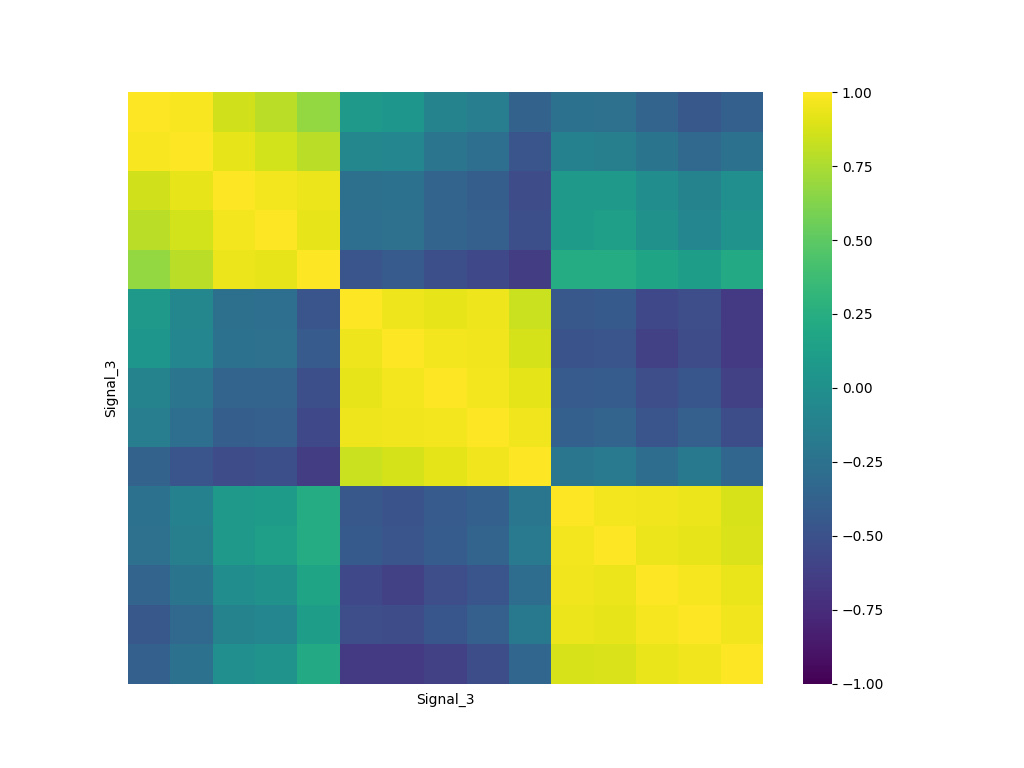
\includegraphics[width=0.45\textwidth]{./picture/systematic/Fragmentation_corr_all.png}
  }
  \hfill
  \subfloat[][Correlation matrix reconstructed using the leading four eigenvectors.]
  {
    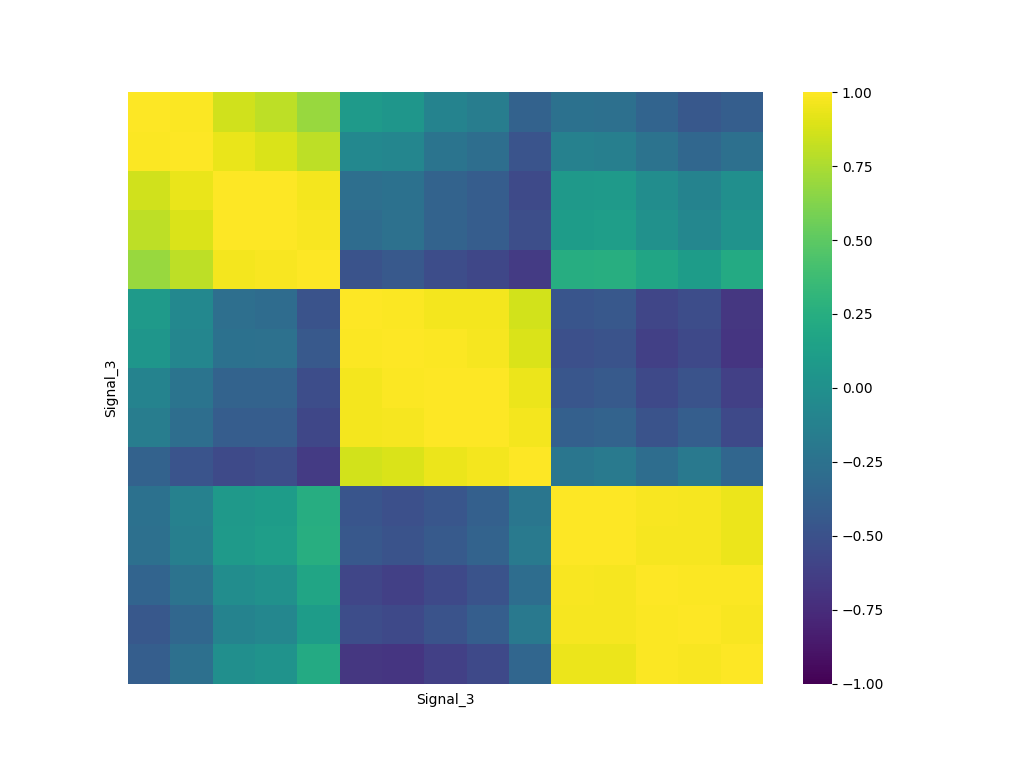
\includegraphics[width=0.45\textwidth]{./picture/systematic/Fragmentation_corr_partial.png}
  }
  \caption{
  Correlation matrices associated with the systematic uncertainty in the fragmentation.
  The left plot is obtained using all eigenvectors, while the right plot is reconstructed using the leading four eigenvectors.
  }
  \label{fig:fragmentation_corr}
\end{figure}

Resonant contributions are not well modeled in \texttt{PYTHIA}.
To check the impact of this mismodelling, the reconstruction efficiency is studied using the $K_{1}(1270)$ resonance.
As described in Appendix~\ref{sec:K1_comparison}, the efficiencies are calculated as functions of $M_{X_{s}}$ for the samples generated with \texttt{PYTHIA} and with the $K_{1}(1270)$ resonance.
The efficiency differences between these two samples are smaller than the differences among decay modes with different multiplicities.
Consequently, among the systematic uncertainties associated with \texttt{PYTHIA} mismodelling, only the uncertainty from the fragmentation is considered.

\section{Background normalization}
As discussed in Section~\ref{sec:validation}, data--MC discrepancies are observed in the event yields in the $M_{\textrm{bc}}$ sideband and the FastBDT sideband.
The data-to-MC ratios in the $M_{\textrm{bc}}$ sideband region are
\begin{linenomath*}
  \begin{equation*}
    \frac{\textrm{Data}}{\textrm{MC}} = 
  \begin{cases}
    1.12 \pm 0.03 & (0.0 < M_{X_{s}}^{\textrm{reco}} < 0.6~\textrm{GeV}/c^{2}), \\[10pt]
    1.04 \pm 0.05 & (0.6 \leq M_{X_{s}}^{\textrm{reco}} < 1.0~\textrm{GeV}/c^{2}), \\[10pt]
    1.10 \pm 0.03 & (1.0 \leq M_{X_{s}}^{\textrm{reco}} < 2.0~\textrm{GeV}/c^{2}),
  \end{cases}
  \end{equation*}
\end{linenomath*}
where only the statistical uncertainties of data and MC are included.
The data-to-MC ratios in the FastBDT sideband region are
\begin{linenomath*}
  \begin{equation*}
    \frac{\textrm{Data}}{\textrm{MC}} = 
  \begin{cases}
    1.11 \pm 0.06 & (0.0 < M_{X_{s}}^{\textrm{reco}} < 0.6~\textrm{GeV}/c^{2}), \\[10pt]
    1.02 \pm 0.07 & (0.6 \leq M_{X_{s}}^{\textrm{reco}} < 1.0~\textrm{GeV}/c^{2}), \\[10pt]
    1.10 \pm 0.04 & (1.0 \leq M_{X_{s}}^{\textrm{reco}} < 2.0~\textrm{GeV}/c^{2}),
  \end{cases}
  \end{equation*}
\end{linenomath*}
where only the statistical uncertainties of data and MC are included.

Conservatively, relative uncertainties of $\pm20\%$ are assigned to the overall background normalization in each $M_{X_{s}}^{\textrm{reco}}$ region.
These uncertainties are applied separately to each background component: charged $B\bar{B}$, mixed $B\bar{B}$, $u\bar{u}$, $d\bar{d}$, $s\bar{s}$, and $c\bar{c}$ templates.

\section{$q\bar{q}$ background shape}
The FastBDT output is used as the fit variable.
There may be discrepancies between data and MC in the FastBDT output.
In this analysis, these discrepancies are corrected by training an additional FastBDT, denoted as BDTc~\cite{Martschei:2012pr}.

BDTc is trained to distinguish off-resonance data from off-resonance MC.
If the MC perfectly models the data, the BDTc output distributions for data and MC should be the same.
However, if there is a data--MC discrepancy, the BDTc output distributions are different.

Figure~\ref{fig:BDTc_distribution} shows the BDTc output distribution for the off-resonance sample.
For each event, a weight of $\sqrt{\frac{p}{1-p}}$ is applied, where $p$ is the BDTc output.
If an event is data-like, the BDTc output is close to 1, and therefore $\sqrt{\frac{p}{1-p}}$ becomes large.
On the other hand, if an event is MC-like, the BDTc output is close to 0, and the weight becomes small.
Consequently, this weight makes the MC distribution more data-like.

After applying the correction, a normalization factor is applied to preserve the total number of events.
Figure~\ref{fig:BDTc_distribution} shows the BDTc output distribution after the correction.
The discrepancy between data and MC is reduced after the correction.
\begin{figure}
    \centering
    \subfloat[][BDTc output distribution for the off-resonance sample before the correction]{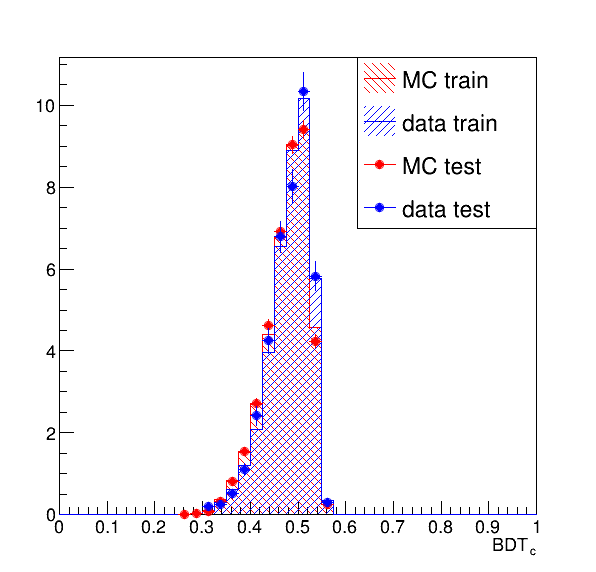
\includegraphics[width=0.45\textwidth]{./picture/systematic/BDTc_BeforeCorrection.png}}
    \hfill
    \subfloat[][BDTc output distribution for the off-resonance sample after the correction]{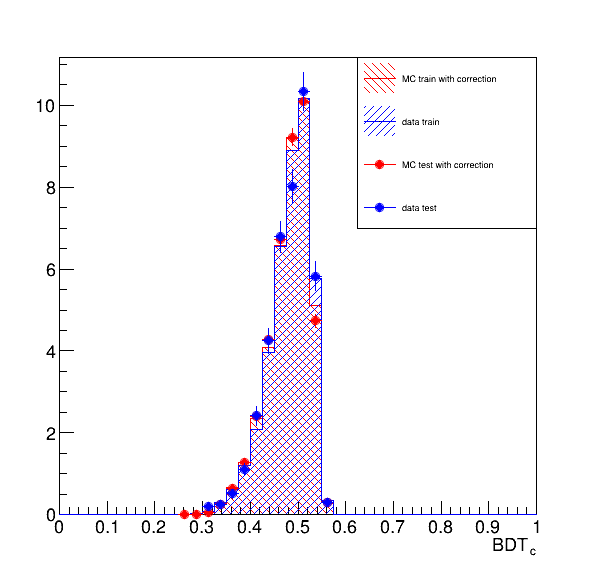
\includegraphics[width=0.45\textwidth]{./picture/systematic/BDTc_AfterCorrection.png}}
    \caption{BDTc output distributions for the off-resonance sample before and after the correction. A weight of $\sqrt{\frac{p}{1-p}}$ is applied for the correction, where $p$ is the BDTc output. After applying the correction, a normalization factor is applied to preserve the total number of events.}
    \label{fig:BDTc_distribution}
\end{figure}

Figure~\ref{fig:BDTc_compare} shows the distributions of selected variables for the off-resonance sample.
The distributions are slightly modified by the BDTc correction.
The FastBDT distribution after the BDTc correction is used to evaluate the systematic uncertainty.
One nuisance parameter is added for this uncertainty.
\begin{figure}
    \centering
    \subfloat{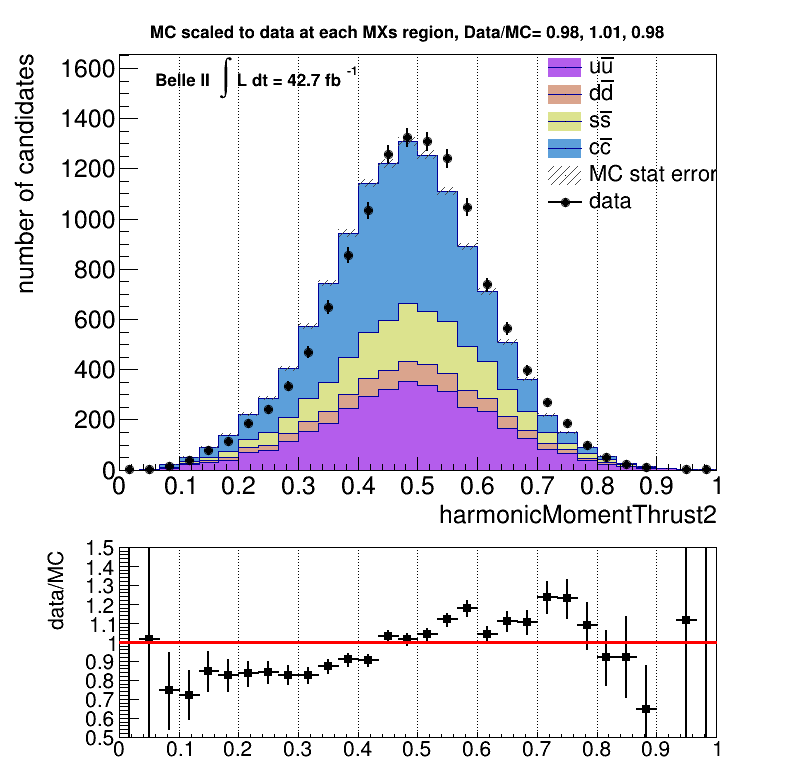
\includegraphics[width=0.3\textwidth]{./picture/off/harmonicMomentThrust2_offres.png}}
    \subfloat{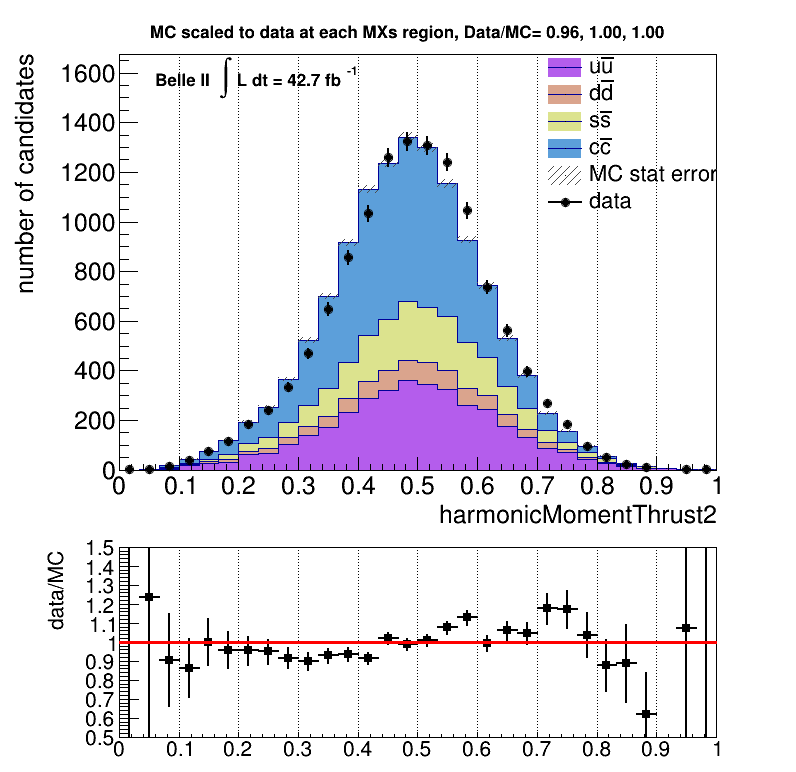
\includegraphics[width=0.3\textwidth]{./picture/off_correction/harmonicMomentThrust2_offres.png}}\\
    \subfloat{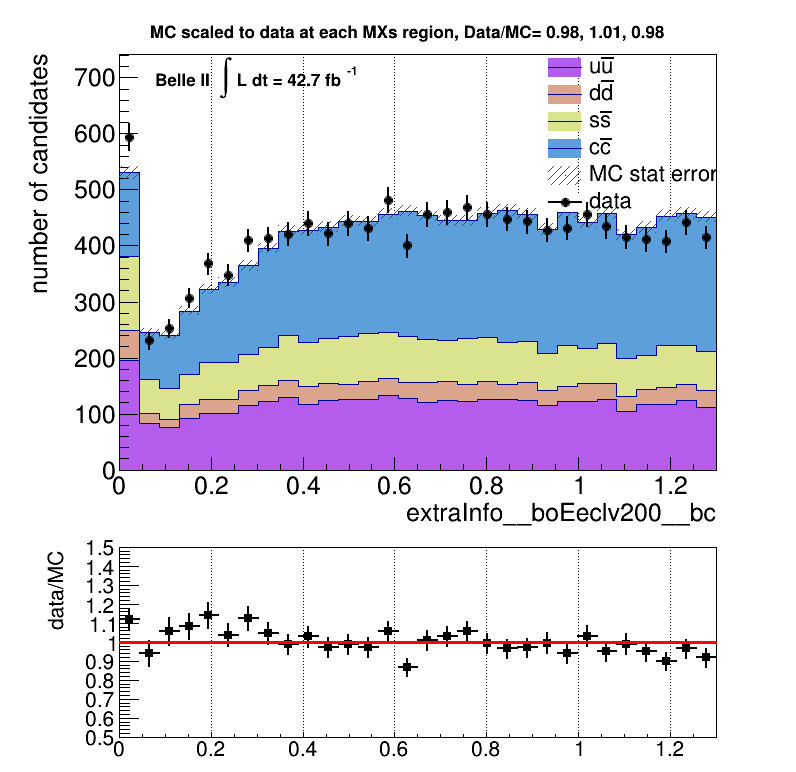
\includegraphics[width=0.3\textwidth]{./picture/off/extraInfo__boEeclv200__bc_offres.png}}
    \subfloat{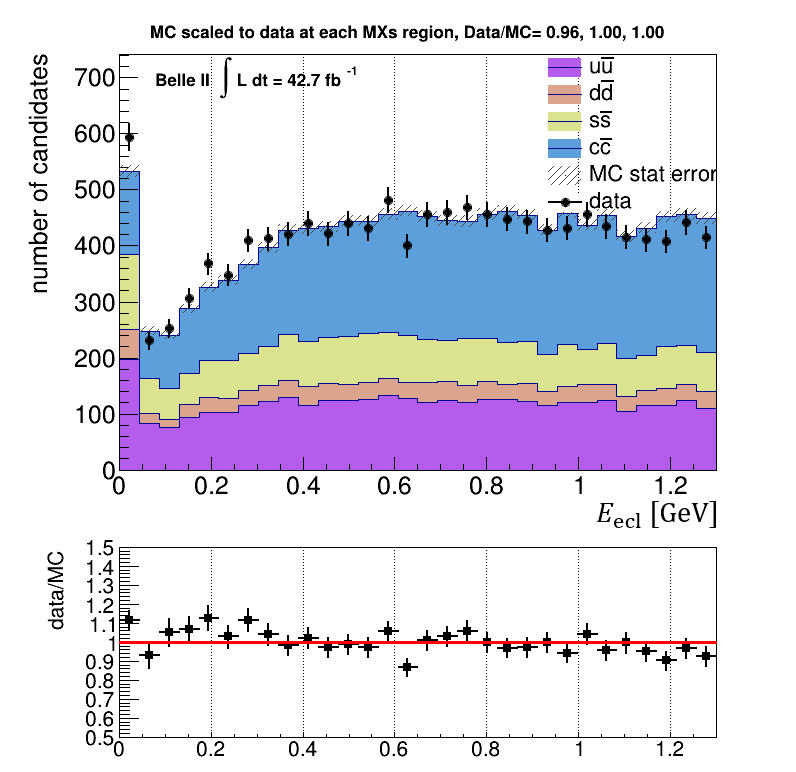
\includegraphics[width=0.3\textwidth]{./picture/off_correction/extraInfo__boEeclv200__bc_offres.png}}\\
    \subfloat{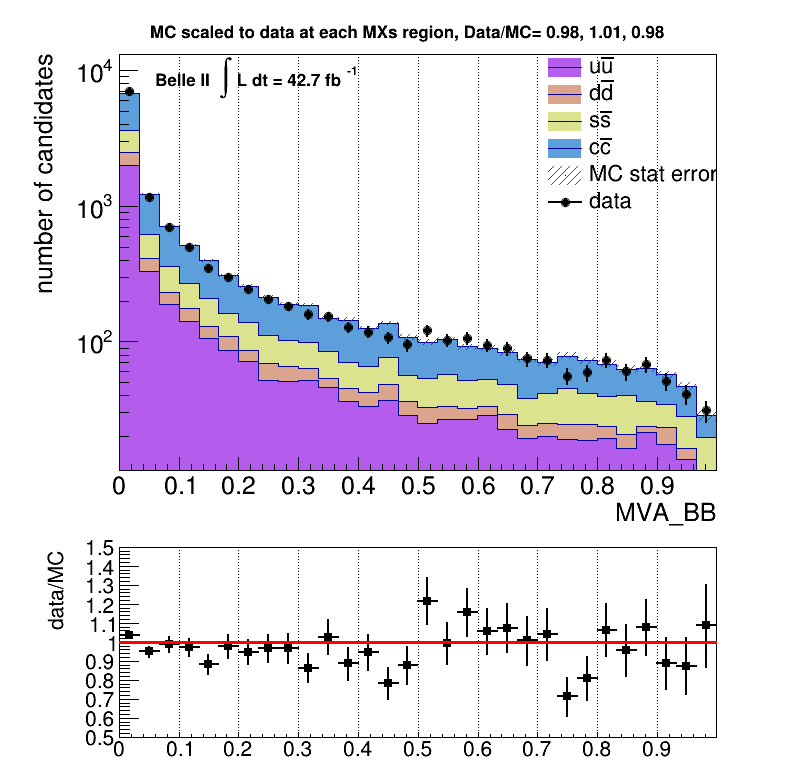
\includegraphics[width=0.3\textwidth]{./picture/off/MVA_BB_offres.png}}
    \subfloat{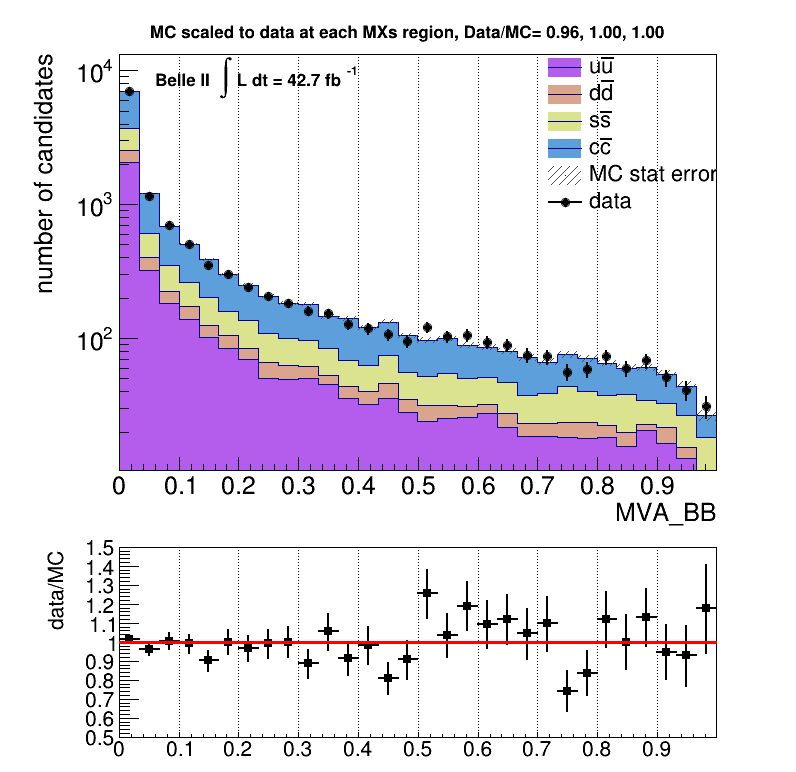
\includegraphics[width=0.3\textwidth]{./picture/off_correction/MVA_BB_offres.png}}
    \caption{Distributions of (top) \texttt{harmonicMomentThrust2}, (middle) $E_{\textrm{ECL}}$, and (bottom) the FastBDT output. The definition of \texttt{harmonicMomentThrust2} is given in Appendix~\ref{sec:FastBDT_inputs}. The plots are obtained from the off-resonance sample. The left plots show the distributions before the BDTc correction, while the right plots show the distributions after the BDTc correction.}
    \label{fig:BDTc_compare}
\end{figure}

\section{$B\bar{B}$ counting}
The number of $\Upsilon(4S)$ events is $N_{\Upsilon(4S)} = (387.1 \pm 5.6) \times 10^{6}$.
Therefore, a relative uncertainty of 1.5\% is assigned due to the uncertainty in the number of $B\bar{B}$ pairs.

\section{Branching ratios of $B$ meson decays}
The branching ratios of $B$ meson decays are determined by the decay files used in \textsc{basf2}.
These values have uncertainties.

Figure~\ref{fig:BBremaindecay} shows the decay modes of $B$ mesons in the charged and mixed $B\bar{B}$ background samples after all selection requirements are applied.
\begin{figure}
    \centering
    \subfloat[Decay modes of the charged $B\bar{B}$ background]{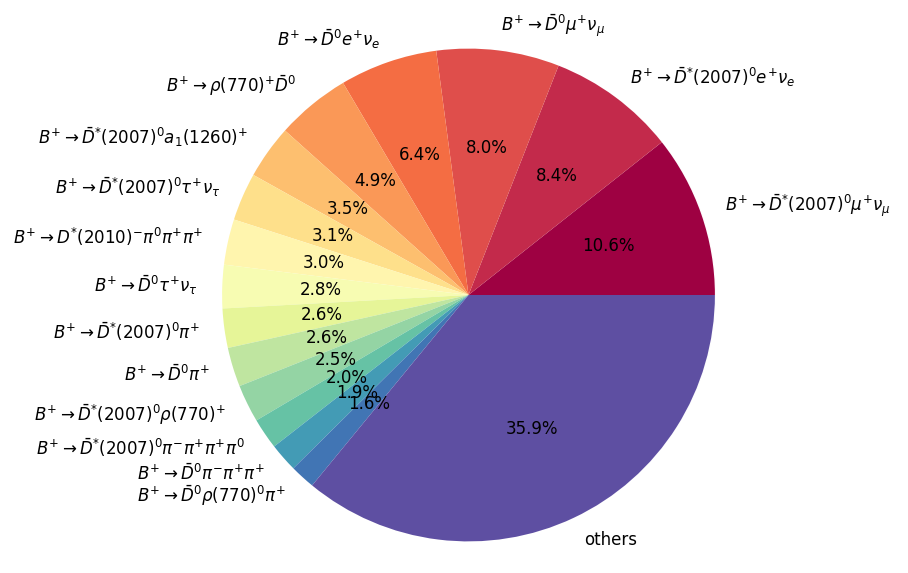
\includegraphics[width=0.45\textwidth]{./picture/systematic/CHG_BKG_PIE.png}}
    \hfill
    \subfloat[Decay modes of the mixed $B\bar{B}$ background]{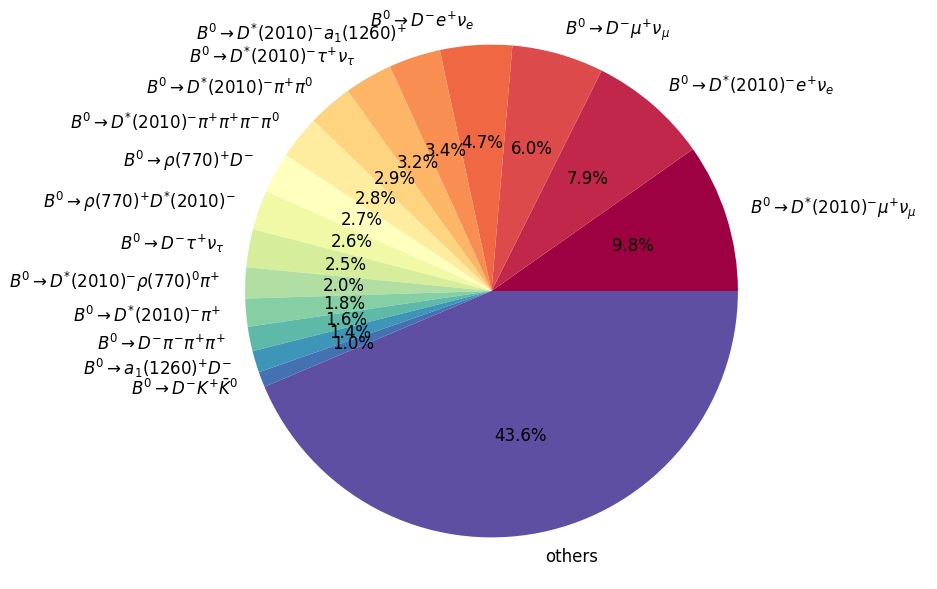
\includegraphics[width=0.45\textwidth]{./picture/systematic/MIX_BKG_PIE.png}}
    \caption{Remaining components of the (a) charged and (b) mixed $B\bar{B}$ backgrounds after all selection requirements are applied. The numbers in the pie charts are given in arbitrary units.}
    \label{fig:BBremaindecay}
\end{figure}

The same procedure described in Section~\ref{sec:hadron_pid_syst} is used to reduce the number of nuisance parameters.

A total of 500 toy samples are generated to estimate the covariance matrix associated with the uncertainties in the $B$ meson branching ratios.
For each toy sample, the branching ratios are varied according to Gaussian distributions defined by their uncertainties from the PDG.
Because this procedure is performed manually, only 70.7\% and 60.1\% of the $B$ meson decays are varied for the charged and mixed backgrounds, respectively.
In addition, $B \rightarrow K K_{L}^{0} K_{L}^{0}$ decays are considered separately to check their impact.

Figure~\ref{fig:BR_corr} shows the correlation matrices obtained using all eigenvectors and using only the leading eight eigenvectors.
The cumulative explained variance ratio for these eight eigenvectors is 0.974.
The leading eight eigenvectors are retained and implemented as independent nuisance parameters in the fit.
\begin{figure}
    \centering
    \subfloat[][Correlation matrix among the fit bins and event categories induced by the uncertainties in the branching ratios.]{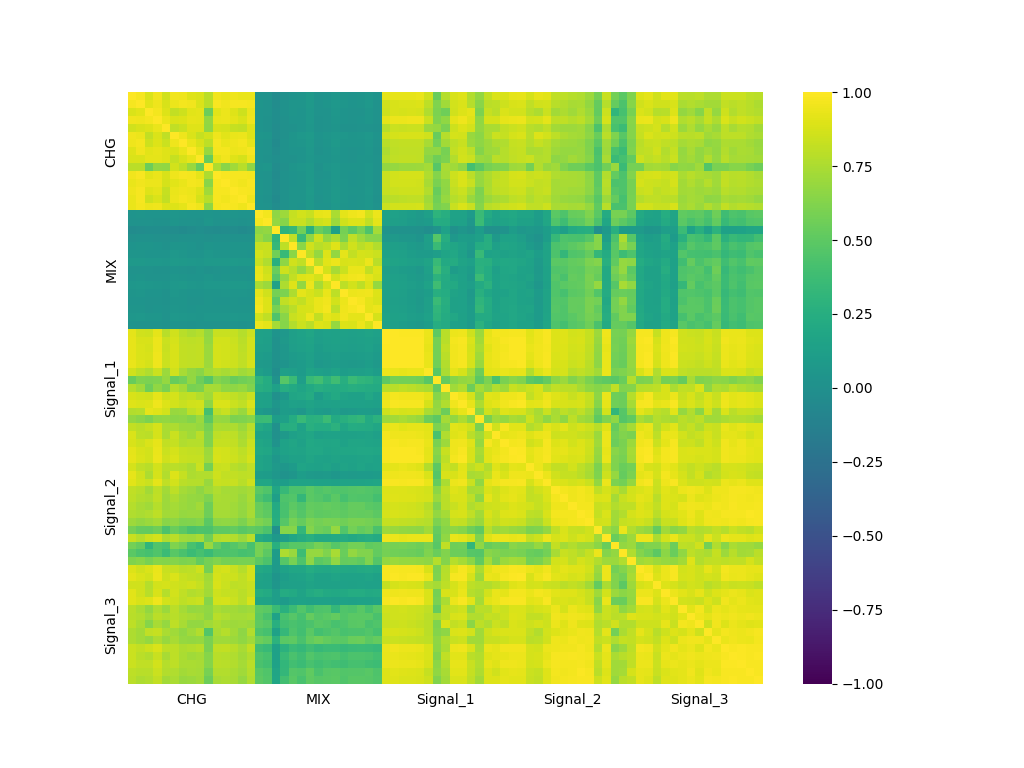
\includegraphics[width=0.45\textwidth]{./picture/systematic/BR_corr_all.png}}
    \hfill
    \subfloat[][Correlation matrix reconstructed using the leading eight eigenvectors.]{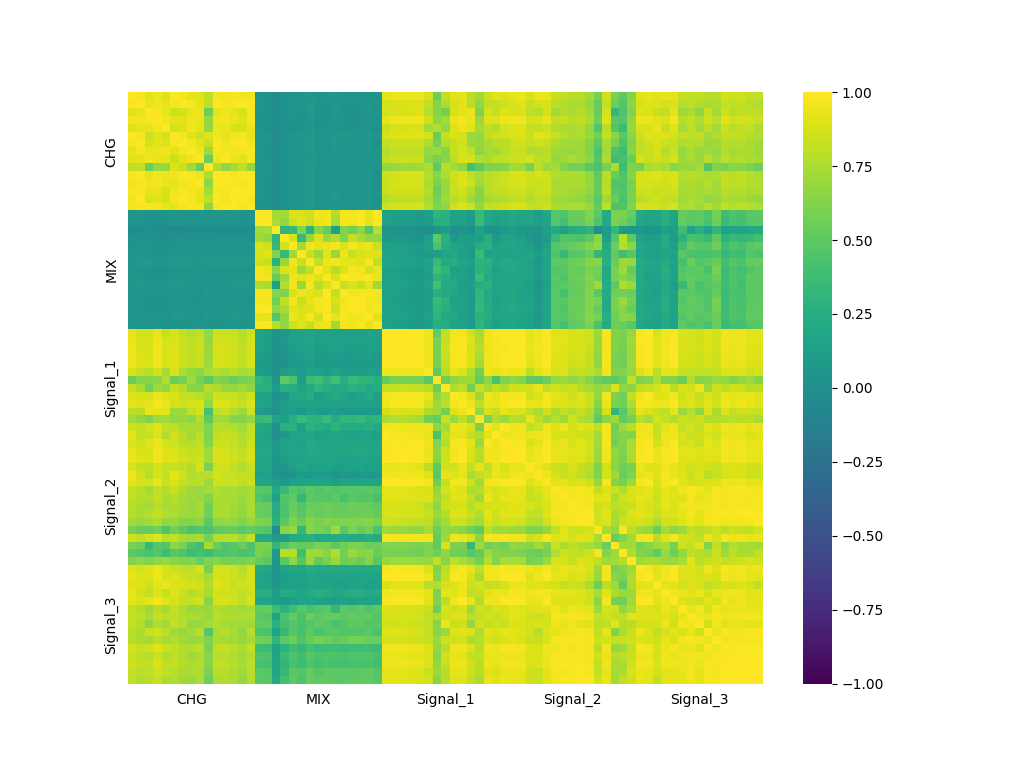
\includegraphics[width=0.45\textwidth]{./picture/systematic/BR_corr_partial.png}}
    \caption{Correlation matrices associated with the systematic uncertainties in the $B$ meson branching ratios. The left plot is obtained using all eigenvectors, while the right plot is reconstructed using the leading eight eigenvectors.}
    \label{fig:BR_corr}
\end{figure}

\section{Mismodelling of $B\rightarrow X_{s} n\bar{n}$ decays}
As discussed in Section~\ref{sec:Xsnnbar_correction}, the $M_{n\bar{n}}$ distribution is modeled in this analysis.
To cover possible mismodelling, a relative uncertainty of $\pm100\%$ is assigned to the branching ratio of $B\rightarrow X_{s} n\bar{n}$ decays.

\section{Mismodelling of $B\rightarrow X_{s} K_{L}^{0} K_{L}^{0}$ decays}
As discussed in Section~\ref{sec:XsKLKL_correct}, the Dalitz-plot distribution is modeled in this analysis.
To cover possible mismodelling, a relative uncertainty of $\pm100\%$ is assigned to the branching ratio of $B\rightarrow X_{s} K_{L}^{0} K_{L}^{0}$ decays.

\section{$D\rightarrow K_{L}^{0}X$ decay from $B$ meson}
As discussed in Section~\ref{sec:DtoKLX_correction}, a scale factor of $1.3\pm0.1$ is applied to $D\rightarrow K_{L}^{0}X$ decays from $B$ mesons.
The uncertainty in this scale factor is adopted as a systematic uncertainty.

\section{$K_{L}^{0}$ ECL efficiency}
In the $B^{+} \rightarrow K^{+} \nu \bar{\nu}$ analysis~\cite{Belle-II:2023esi}, the $K_{L}^{0}$ reconstruction efficiency as the ECL cluster had a significant impact on the result for the inclusive-tag analysis.
For the hadronic-tag analysis, however, this effect is not dominant.

In this analysis, ECL clusters are investigated.
Only $\mathcal{O}(0.1\%)$ of ECL clusters originate from $K_{L}^{0}$.
Therefore, no correction is applied.
Instead, a relative uncertainty of $\pm17\%$ is assigned to events containing ECL clusters originating from $K_{L}^{0}$.
This uncertainty is motivated by the hadronic-tag $B^{+} \rightarrow K^{+} \nu \bar{\nu}$ analysis~\cite{Belle-II:2023esi}.

\section{Uncorrelated uncertainties}
As discussed in Section~\ref{sec:systematic_uncertainty} and Eq.~\ref{eq:PCA_approximation}, PCA is performed for some systematic uncertainties, and the dominant eigenvectors are retained.
The remaining component of the covariance matrix is approximated by a diagonal matrix.
The diagonal elements are adopted as uncorrelated bin-by-bin uncertainties.
To reduce the number of nuisance parameters, these uncorrelated uncertainties are added in quadrature to the MC statistical uncertainties.

\section{Summary}
Table~\ref{tab:uncertaintiestable} summarizes the systematic uncertainties
and the statistical uncertainty from the MC samples.
Here, $\sigma_{\mu_{1}}$, $\sigma_{\mu_{2}}$, and $\sigma_{\mu_{3}}$ denote the uncertainties in $\mu_{1}$, $\mu_{2}$, and $\mu_{3}$, respectively.
To evaluate the impact of each systematic source on $\sigma_{\mu}$, a fit to the Asimov dataset with $\mu=1$ is performed.
The asymmetric \texttt{MINOS} errors from the fit are taken as the uncertainties in $\mu$.
To estimate the contribution from a specific nuisance parameter, the fit to the Asimov dataset is repeated with that nuisance parameter removed.
The uncertainty from the specific nuisance parameter is then calculated as
\begin{align}
    \label{eq:syst_break}
    \sigma_{\textrm{total}} = \sqrt{\sigma_{\textrm{without syst}}^{2} + \sigma_{\textrm{syst}}^{2}},
\end{align}
where $\sigma_{\textrm{total}}$ is the uncertainty obtained with all nuisance parameters included, $\sigma_{\textrm{without syst}}$ is the uncertainty obtained with the specific nuisance parameter removed, and $\sigma_{\textrm{syst}}$ is the contribution from that nuisance parameter.

In the table, the asymmetric \texttt{MINOS} errors are first symmetrized by taking the average of the absolute values of the positive and negative errors.
The contribution from each systematic source is then calculated using the symmetrized uncertainties.

The statistical uncertainty is estimated by fixing all nuisance parameters.
The resulting statistical uncertainty is also shown in Table~\ref{tab:uncertaintiestable}.

\begin{table}
\caption{Summary of the systematic uncertainties and statistical uncertainty. The values are obtained using the Asimov dataset.}
  \renewcommand{\arraystretch}{1.4}
  \centering
\begin{tabular}{ p{6cm} p{2.5cm} p{2.5cm} p{2.5cm}}
 \hline
  \hline
Source &  Impact on $\sigma_{\mu_{1}}$ & Impact on $\sigma_{\mu_{2}}$ & Impact on $\sigma_{\mu_{3}}$\\
 \hline
Background normalization & 1.17 & 2.22 & 3.96 \\
MC statistics & 0.87 & 1.55 & 3.47 \\
FastBDT efficiency & 0.09 & 0.34 & 1.27 \\
$K^{*}-X_{s}$ transition & 0.01 & 0.02 & 1.17 \\
BR of main $B$ meson decays & 0.28 & 0.65 & 1.05 \\
Photon multiplicity & 0.08 & 0.24 & 0.95 \\
$q\bar{q}$ efficiency & 0.20 & 0.25 & 0.93 \\
Additional FEI uncertainty & 0.18 & 0.34 & 0.55 \\
$q\bar{q}$ shape & 0.25 & 0.26 & 0.52 \\
Fragmentation of $X_{s}$ & 0.01 & 0.05 & 0.44 \\
FEI calibration for $B\bar{B}$ & 0.19 & 0.28 & 0.42 \\
Fermi motion momentum & 0.00 & 0.00 & 0.39 \\
Mismodelling of $B \rightarrow X_{s} K_{L}^{0} K_{L}^{0}$ & 0.02 & 0.41 & 0.35 \\
$B\rightarrow K^{*}$ form factor & 0.01 & 0.44 & 0.32 \\
$B\bar{B}$ counting & 0.05 & 0.12 & 0.30 \\
Fraction of decay modes & 0.14 & 0.24 & 0.25 \\
b-quark mass & 0.00 & 0.00 & 0.19 \\
$B\rightarrow K$ form factor & 0.15 & 0.00 & 0.14 \\
Pion ID & 0.01 & 0.09 & 0.14 \\
BR of $D \rightarrow K_{L}^{0} X$ from B meson & 0.02 & 0.12 & 0.11 \\
Tracking efficiency & 0.01 & 0.02 & 0.09 \\
$\pi^{0}$ efficiency & 0.01 & 0.04 & 0.08 \\
Mismodelling of $B\rightarrow X_{s} n\bar{n}$ & 0.15 & 0.52 & 0.04 \\
$K_{L}^{0}$ ECL efficiency & 0.01 & 0.02 & 0.04 \\
$K_{S}^{0}$ efficiency & 0.01 & 0.03 & 0.04 \\
Kaon ID & 0.06 & 0.02 & 0.03 \\
\hline
Statistical uncertainty & 1.65 & 2.86 & 5.43 \\
         \hline
            \hline
\end{tabular}
    \label{tab:uncertaintiestable}
\end{table}

\section{Fit bias}
As discussed in Sections~\ref{sec:fit_quality} and~\ref{sec:unblind_result}, a bias associated with the fitter is observed.
This effect is included as a systematic uncertainty.
However, to quantify its impact precisely, the uncertainty is assigned only after unblinding the signal region.

\chapter{Fit quality check}
\label{sec:fit_quality}
In this section, the fitter bias is investigated using toy MC studies and linearity tests.

\section{Toy MC study}
To check the quality of the fitter, toy MC studies are performed.
Toy MC samples are generated based on the signal and background histogram templates expected from simulation.
A total of 10000 toy MC experiments are performed.
In each experiment, the numbers of signal and background events are sampled from Poisson distributions whose means are fixed to the expected numbers of events from simulation.
The nuisance parameters associated with the systematic uncertainties are sampled from Gaussian distributions.

Because the number of bins is small, a bias can arise in the pull distribution when a symmetric error is used.
Therefore, the pull is calculated using the asymmetric \texttt{MINOS} errors~\cite{pull}:
\begin{equation}
    \label{eq:pull_equation}
    \textrm{pull} = 
  \begin{cases}
  \frac{(\textrm{true value of $\mu$}) - (\textrm{fit result of $\mu$})}{(\textrm{positive MINOS error of $\mu$})} &\text{if } (\textrm{fit result}) \le (\textrm{true value}) \\[10pt]
  \frac{(\textrm{fit result of $\mu$}) - (\textrm{true value of $\mu$})}{(\textrm{negative MINOS error of $\mu$})} &\text{otherwise},
  \end{cases}
\end{equation}
Figures~\ref{fig:toymc_MXs1}--\ref{fig:toymc_MXs3} show the results of the toy MC studies for the three signal-strength parameters:
$\mu_{1}$, $\mu_{2}$, and $\mu_{3}$.
\begin{figure}
    \centering
    \subfloat[][Distribution of $\mu_{1}$]{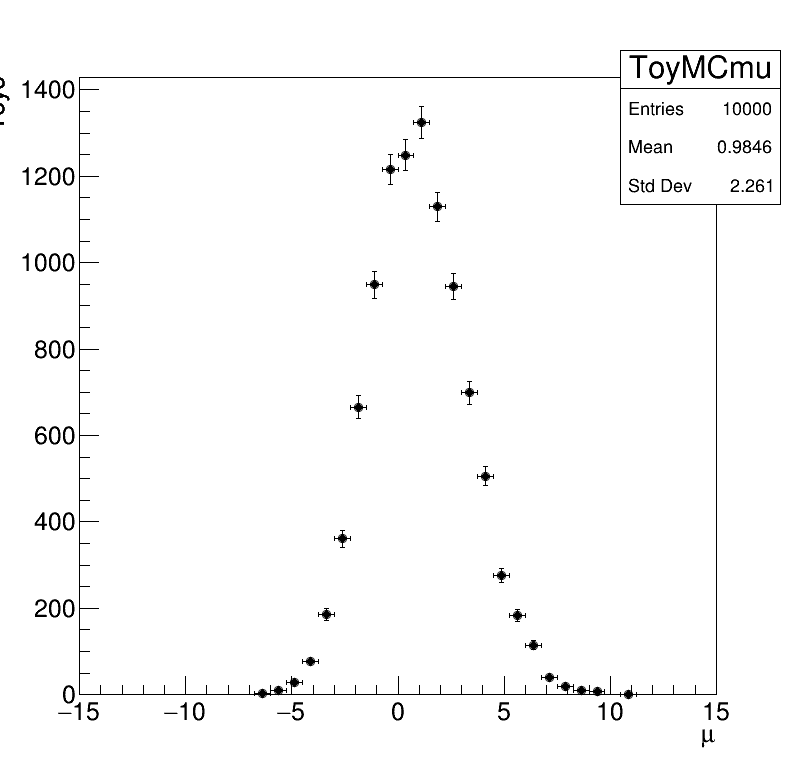
\includegraphics[width=0.3\textwidth]{./picture/TOY/TOYMC_mu_MXs1.png}}
    \subfloat[][Pull of $\mu_{1}$]{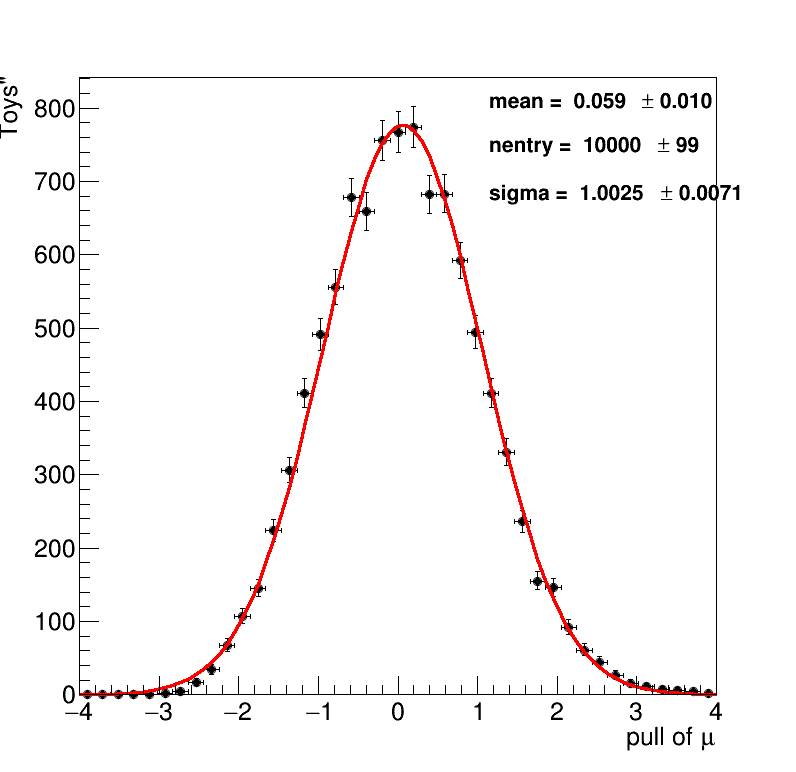
\includegraphics[width=0.3\textwidth]{./picture/TOY/TOYMC_mu_MXs1_pull.png}}\\
    \subfloat[][Positive error of $\mu_{1}$]{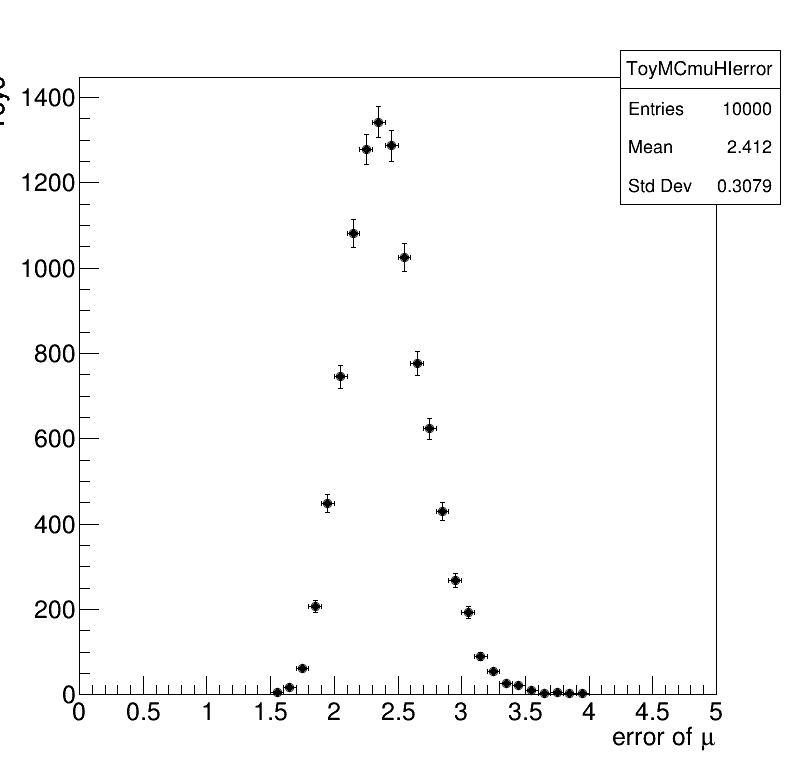
\includegraphics[width=0.3\textwidth]{./picture/TOY/TOYMC_mu_MXs1_HIerror.png}}
    \subfloat[][Negative error of $\mu_{1}$]{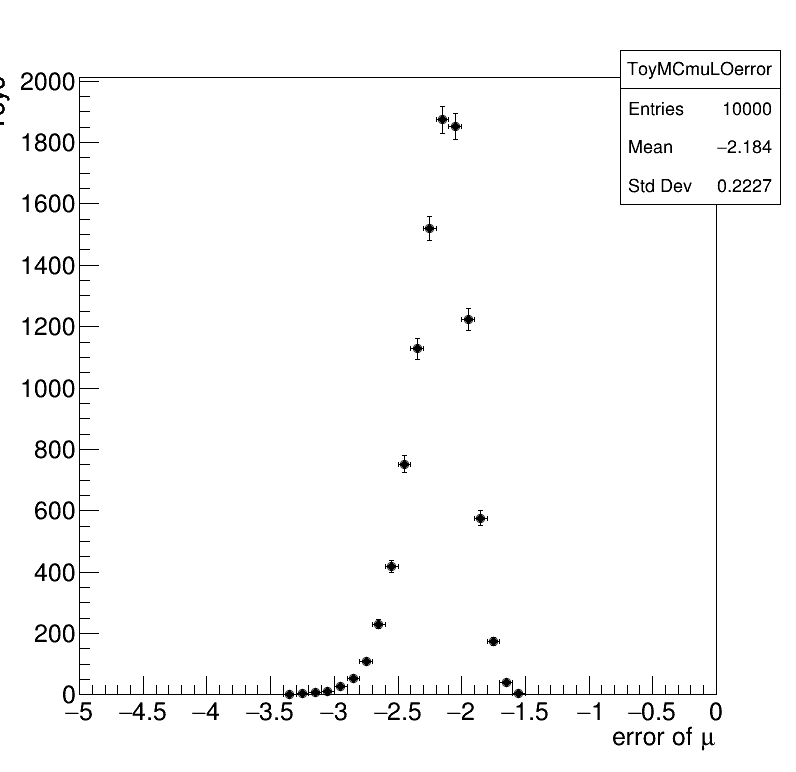
\includegraphics[width=0.3\textwidth]{./picture/TOY/TOYMC_mu_MXs1_LOerror.png}}
    \caption{Results of 10000 toy MC experiments for $0.0 < M_{X_{s}} < 0.6~\textrm{GeV}/c^{2}$.}
    \label{fig:toymc_MXs1}
\end{figure}
\begin{figure}
  \centering
  \subfloat[][Distribution of $\mu_{2}$]{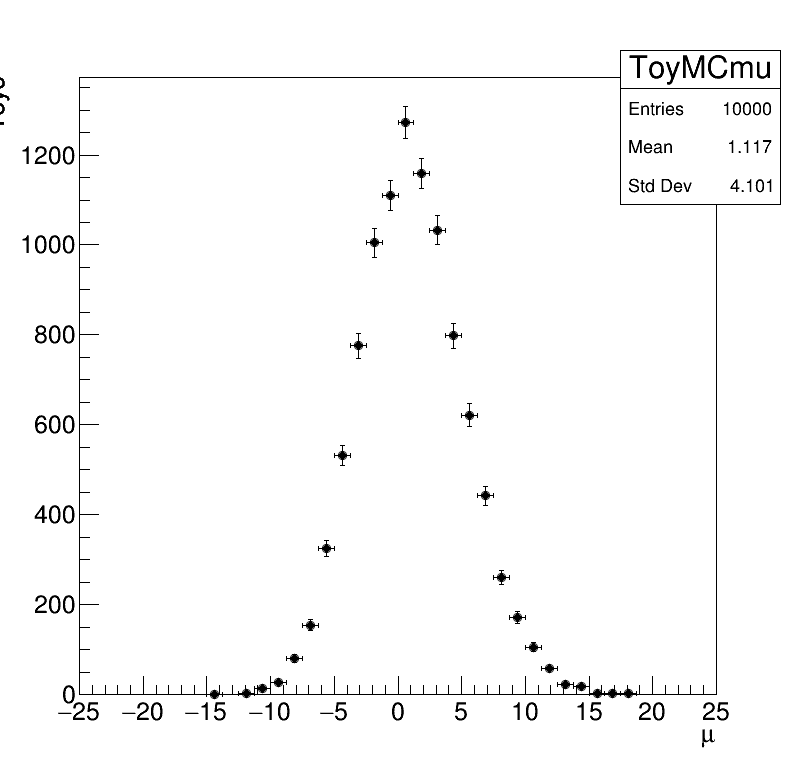
\includegraphics[width=0.3\textwidth]{./picture/TOY/TOYMC_mu_MXs2.png}}
  \subfloat[][Pull of $\mu_{2}$]{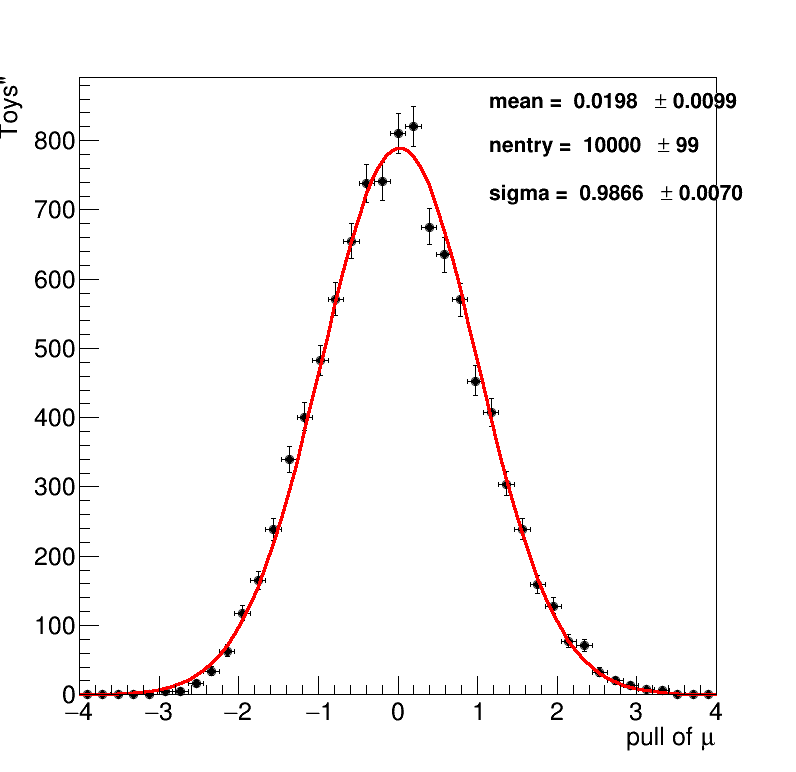
\includegraphics[width=0.3\textwidth]{./picture/TOY/TOYMC_mu_MXs2_pull.png}}\\
  \subfloat[][Positive error of $\mu_{2}$]{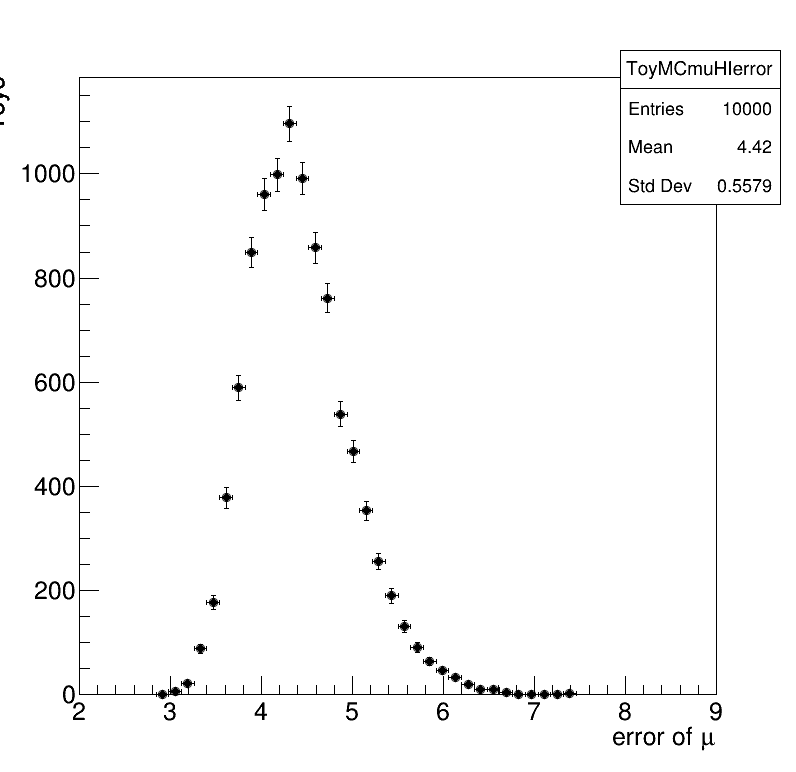
\includegraphics[width=0.3\textwidth]{./picture/TOY/TOYMC_mu_MXs2_HIerror.png}}
  \subfloat[][Negative error of $\mu_{2}$]{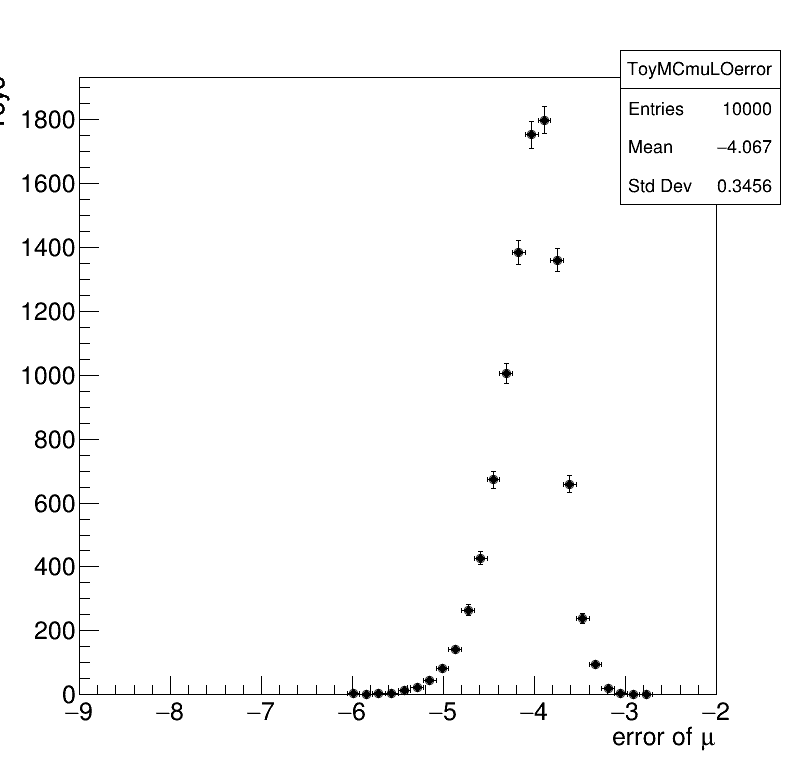
\includegraphics[width=0.3\textwidth]{./picture/TOY/TOYMC_mu_MXs2_LOerror.png}}
  \caption{Results of 10000 toy MC experiments for $0.6 < M_{X_{s}} < 1.0~\textrm{GeV}/c^{2}$.}
  \label{fig:toymc_MXs2}
\end{figure}
\begin{figure}
  \centering
  \subfloat[][Distribution of $\mu_{3}$]{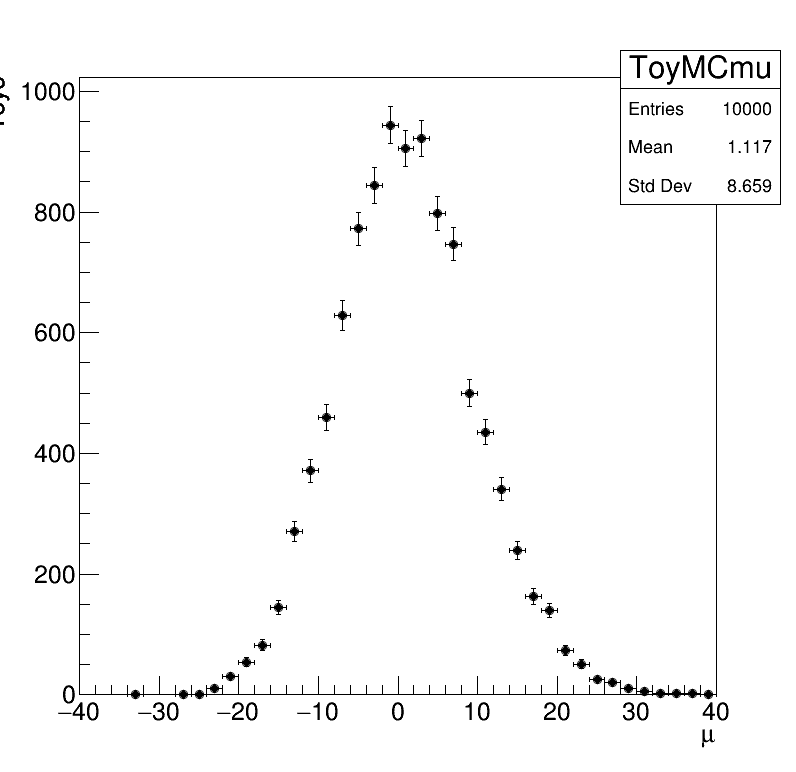
\includegraphics[width=0.3\textwidth]{./picture/TOY/TOYMC_mu_MXs3.png}}
  \subfloat[][Pull of $\mu_{3}$]{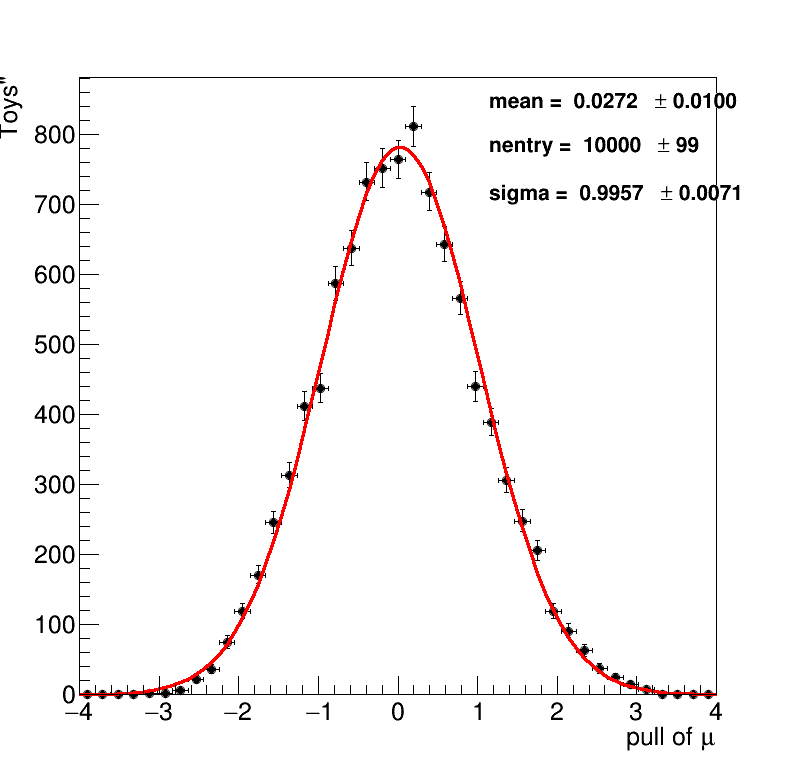
\includegraphics[width=0.3\textwidth]{./picture/TOY/TOYMC_mu_MXs3_pull.png}}\\
  \subfloat[][Positive error of $\mu_{3}$]{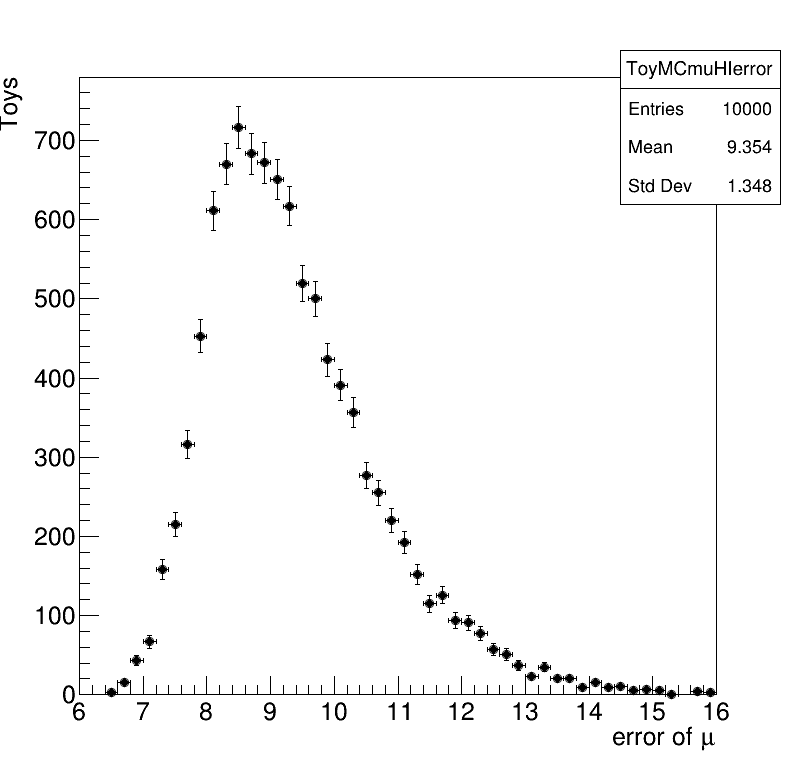
\includegraphics[width=0.3\textwidth]{./picture/TOY/TOYMC_mu_MXs3_HIerror.png}}
  \subfloat[][Negative error of $\mu_{3}$]{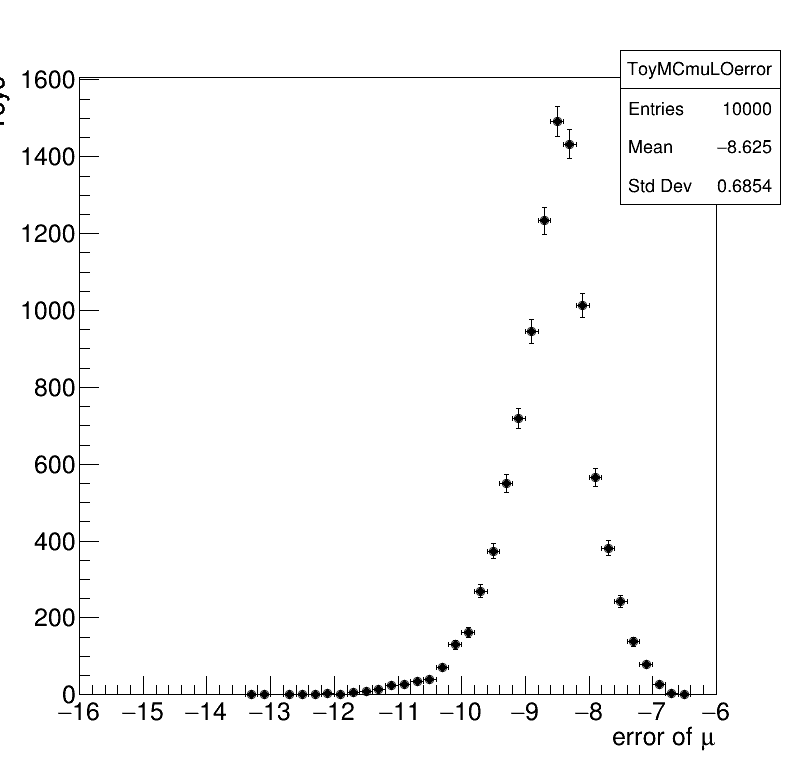
\includegraphics[width=0.3\textwidth]{./picture/TOY/TOYMC_mu_MXs3_LOerror.png}}
  \caption{Results of 10000 toy MC experiments for $1.0~\textrm{GeV}/c^{2} < M_{X_{s}}$.}
  \label{fig:toymc_MXs3}
\end{figure}

To quantify the agreement between the pull distributions and the standard normal distribution, the pull distributions are fitted with Gaussian functions.
The means of the pull distributions are
\begin{equation}
    \textrm{mean} = 
  \begin{cases}
  0.059 \pm 0.010 &(0.0 < M_{X_{s}} < 0.6~\textrm{GeV}/c^{2}), \\[10pt]
  0.020 \pm 0.010 &(0.6 < M_{X_{s}} < 1.0~\textrm{GeV}/c^{2}), \\[10pt]
  0.027 \pm 0.010 &(1.0~\textrm{GeV}/c^{2} < M_{X_{s}}).
  \end{cases}
\end{equation}
The widths of the pull distributions are
\begin{equation}
    \textrm{width} = 
  \begin{cases}
  1.003 \pm 0.007 &(0.0 < M_{X_{s}} < 0.6~\textrm{GeV}/c^{2}), \\[10pt]
  0.987 \pm 0.007 &(0.6 < M_{X_{s}} < 1.0~\textrm{GeV}/c^{2}), \\[10pt]
  0.996 \pm 0.007 &(1.0~\textrm{GeV}/c^{2} < M_{X_{s}}).
  \end{cases}
\end{equation}
In general, the pull distributions show good agreement with the standard normal distribution.

\section{Linearity test}
It is also important to check the linearity of the fitter.
To correctly interpret possible effects from new physics, the fitted signal strength should be proportional to the injected signal strength.

Linearity tests are performed by varying the injected value of $\mu$ from 0 to 10.
In total, 11 different values of $\mu$ are tested.
For each injected value of $\mu$, 10000 toy MC experiments are performed.
Therefore, a total of $11 \times 10000 = 110000$ toy MC experiments are performed.
For each injected value of $\mu$, the median value of the $\mu$ distribution is obtained.
Figure~\ref{fig:Linearitytest} shows the median fitted values for each injected value of $\mu_{1}$, $\mu_{2}$, and $\mu_{3}$.
\begin{figure}
    \centering
    \subfloat[][$0.0 < M_{X_{s}}^{\textrm{true}} < 0.6~\textrm{GeV}$]{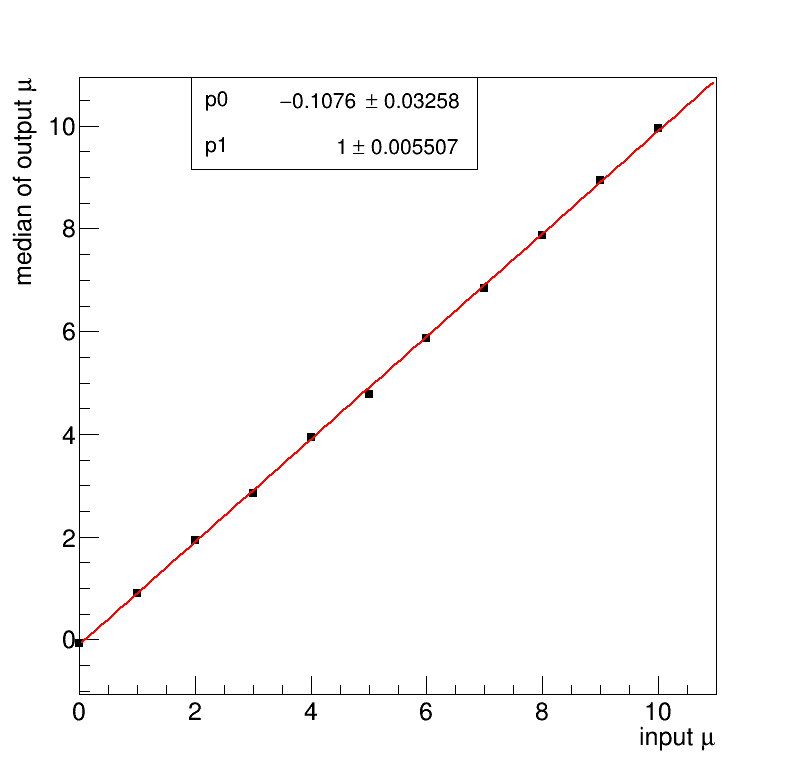
\includegraphics[width=0.3\textwidth]{./picture/LT/Linearity_MXs1_test_median.png}}
    \subfloat[][$0.6 < M_{X_{s}}^{\textrm{true}} < 1.0~\textrm{GeV}$]{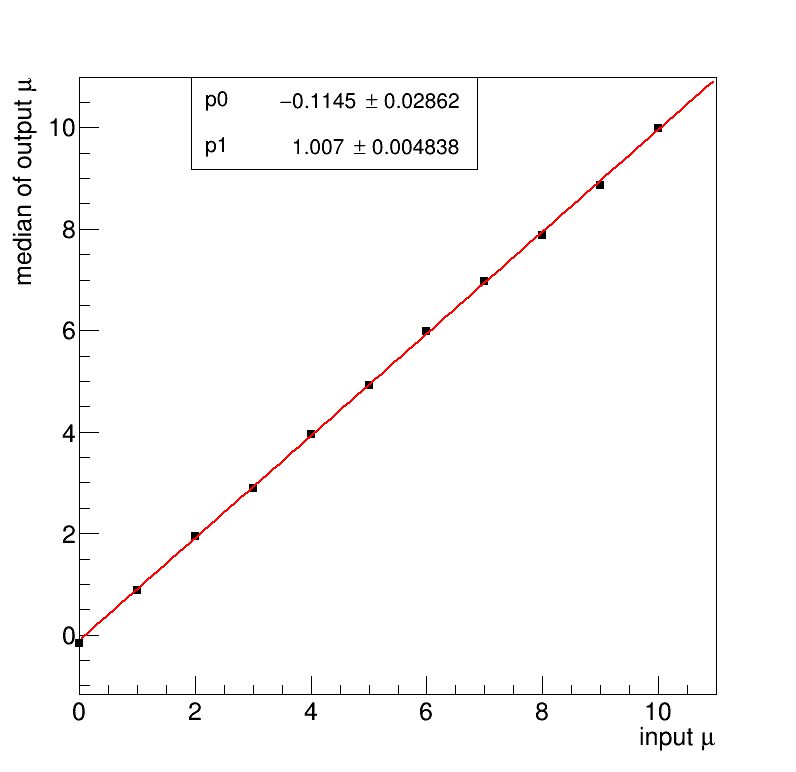
\includegraphics[width=0.3\textwidth]{./picture/LT/Linearity_MXs2_test_median.png}}
    \subfloat[][$1.0~\textrm{GeV} < M_{X_{s}}^{\textrm{true}}$]{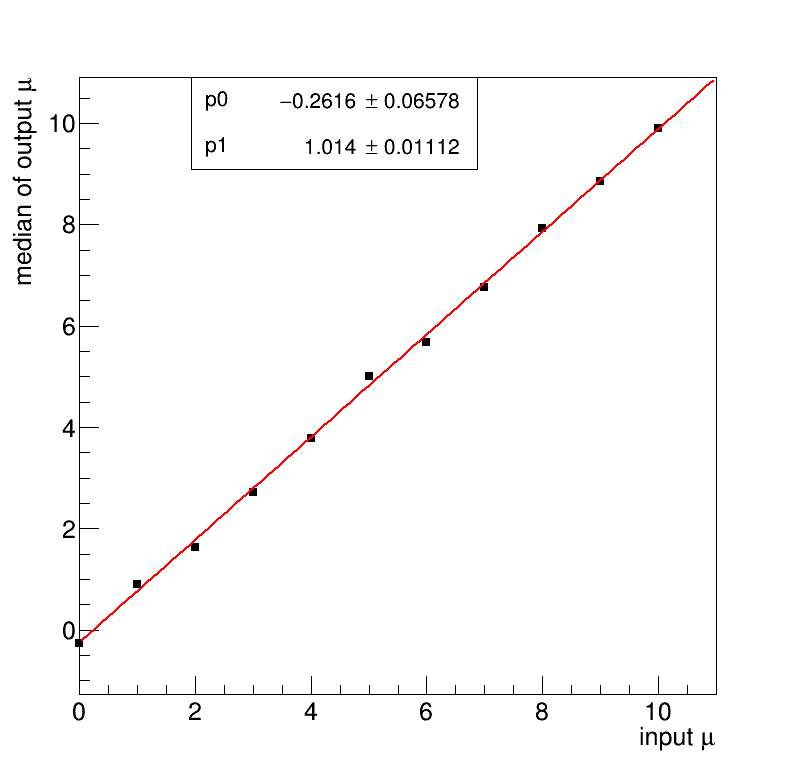
\includegraphics[width=0.3\textwidth]{./picture/LT/Linearity_MXs3_test_median.png}}
    \caption{Results of the linearity tests for the three signal-strength parameters. Each point shows the median value of the fitted $\mu$ distribution.}
    \label{fig:Linearitytest}
\end{figure}
To quantify the linearity of the fitter, the results of the linearity tests are fitted with first-order polynomials.
The fit results are
\begin{equation}
    y = 
  \begin{cases}
    1.00 \cdot x -0.11 & (0.0 < M_{X_{s}} < 0.6~\textrm{GeV}/c^{2}), \\[10pt]
    1.01 \cdot x - 0.11 & (0.6 < M_{X_{s}} < 1.0~\textrm{GeV}/c^{2}), \\[10pt]
    1.01 \cdot x - 0.26 & (1.0~\textrm{GeV}/c^{2} < M_{X_{s}}).
  \end{cases}
\end{equation}
The slopes are in good agreement with unity, while the intercepts show some deviations from zero.

\section{Summary}
A small fitter bias is observed.
To account for this bias, additional post-unblinding systematic uncertainties are assigned.
These post-unblinding systematic uncertainties are discussed in Section~\ref{sec:unblind_result}.

\chapter{Results}
\section{Results of MC study}
Using the Asimov dataset with $\mu=1$, the expected upper limits are
\begin{equation}
    UL(\mu) = 
  \begin{cases}
    4.80 & (0.0 < M_{X_{s}} < 0.6~\textrm{GeV}/c^{2}), \\[10pt]
    8.16 & (0.6 < M_{X_{s}} < 1.0~\textrm{GeV}/c^{2}), \\[10pt]
    16.75 & (1.0~\textrm{GeV}/c^{2} < M_{X_{s}}).
  \end{cases}
\end{equation}
These limits can be converted into branching-ratio upper limits as
\begin{align}
    UL(B\rightarrow X_{s}\nu \bar{\nu}) = BR(B\rightarrow X_{s}\nu \bar{\nu})_{SM} \times UL(\mu),
\end{align}
where $UL(B\rightarrow X_{s}\nu \bar{\nu})$ is the branching-ratio upper limit, $BR(B\rightarrow X_{s}\nu \bar{\nu})_{\mathrm{SM}}$ is the SM prediction for the branching ratio, and $UL(\mu)$ is the upper limit on $\mu$ in each $M_{X_{s}}$ region.
The value of $BR(B\rightarrow X_{s}\nu \bar{\nu})_{\mathrm{SM}}$ in each $M_{X_{s}}$ region is calculated from the signal MC sample based on the Standard Model.

In the MC, the expected branching ratios are 
\begin{equation}
    \label{eq:BR_partial}
    BR(B\rightarrow X_{s}\nu \bar{\nu})_{SM} = \frac{N_{B \rightarrow X_{s} \nu \bar{\nu}}}{N_{B}} =
  \begin{cases}
    4.85 \times 10^{-6} & (0.0 < M_{X_{s}} < 0.6~\textrm{GeV}/c^{2}), \\[10pt]
    8.50 \times 10^{-6} & (0.6 < M_{X_{s}} < 1.0~\textrm{GeV}/c^{2}), \\[10pt]
    15.67 \times 10^{-6} & (1.0~\textrm{GeV}/c^{2} < M_{X_{s}}),
  \end{cases}
\end{equation}
where $N_{B \rightarrow X_{s} \nu \bar{\nu}}$ is the number of $B$ mesons that decay into $X_{s}\nu\bar{\nu}$ in a given $M_{X_{s}}$ region, and $N_B$ is the total number of $B$ mesons.
The corresponding branching-ratio upper limits are
\begin{equation}
    UL(B\rightarrow X_{s}\nu \bar{\nu}) = 
  \begin{cases}
    2.33 \times 10^{-5} & (0.0 < M_{X_{s}} < 0.6~\textrm{GeV}/c^{2}), \\[10pt]
    6.93 \times 10^{-5} & (0.6 < M_{X_{s}} < 1.0~\textrm{GeV}/c^{2}), \\[10pt]
    26.25 \times 10^{-5} & (1.0~\textrm{GeV}/c^{2} < M_{X_{s}}).
  \end{cases}
\end{equation}
Figure~\ref{fig:CLs_asimov} shows the results of the $CL_{s}$ method using
the Asimov dataset.
\begin{figure}
    \centering
    \subfloat[][$0.0 < M_{X_{s}} < 0.6~\textrm{GeV}/c^{2}$]
    {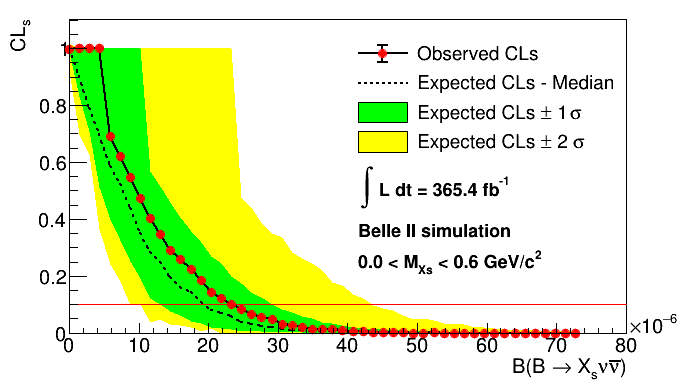
\includegraphics[width=0.47\textwidth]{./picture/UL_MXs1_asimov.png}}
    \subfloat[][$0.6 < M_{X_{s}} < 1.0~\textrm{GeV}/c^{2}$]
    {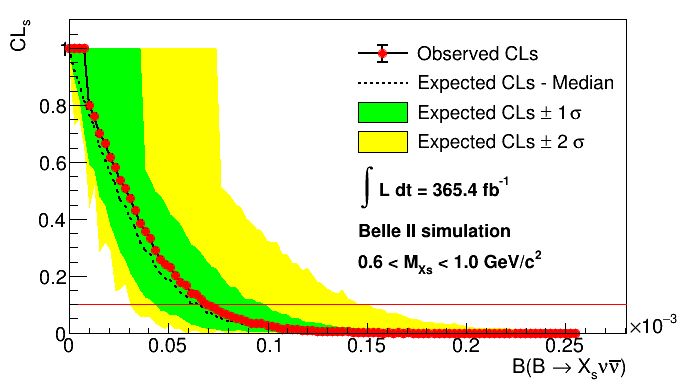
\includegraphics[width=0.47\textwidth]{./picture/UL_MXs2_asimov.png}}\\
    \subfloat[][$1.0~\textrm{GeV}/c^{2} < M_{X_{s}}$]
    {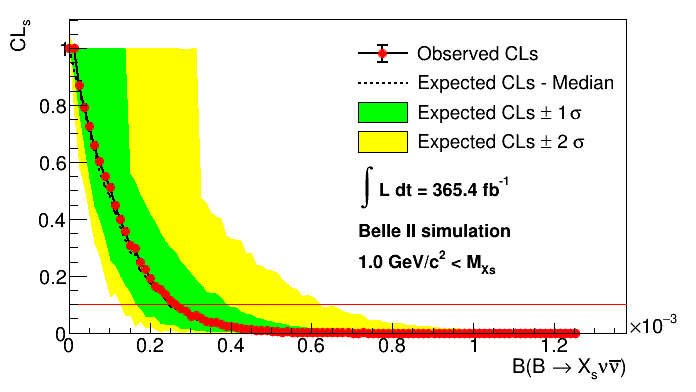
\includegraphics[width=0.47\textwidth]{./picture/UL_MXs3_asimov.png}}
    \subfloat[][Full $M_{X_{s}}$ range]
    {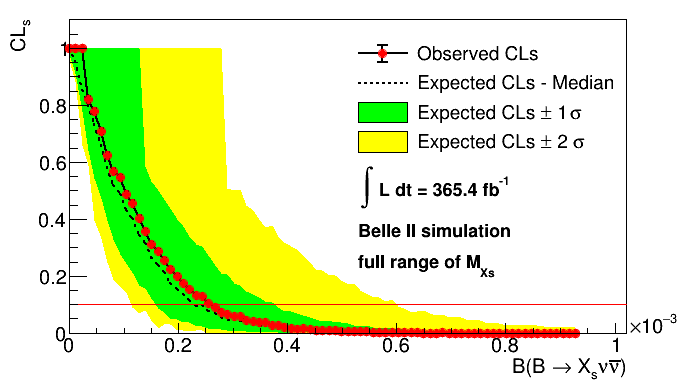
\includegraphics[width=0.47\textwidth]{./picture/UL_mu_sum_asimov.png}}
    \caption{
    $CL_{s}$ values as functions of the tested branching ratio, obtained
    using the Asimov dataset.
    }
    \label{fig:CLs_asimov}
\end{figure}

\section{Post-unblinding results}
\label{sec:unblind_result}
Figure~\ref{fig:bin_index_prefit} shows the bin-index distribution before the fit.
\begin{figure}
  \centering
  \subfloat{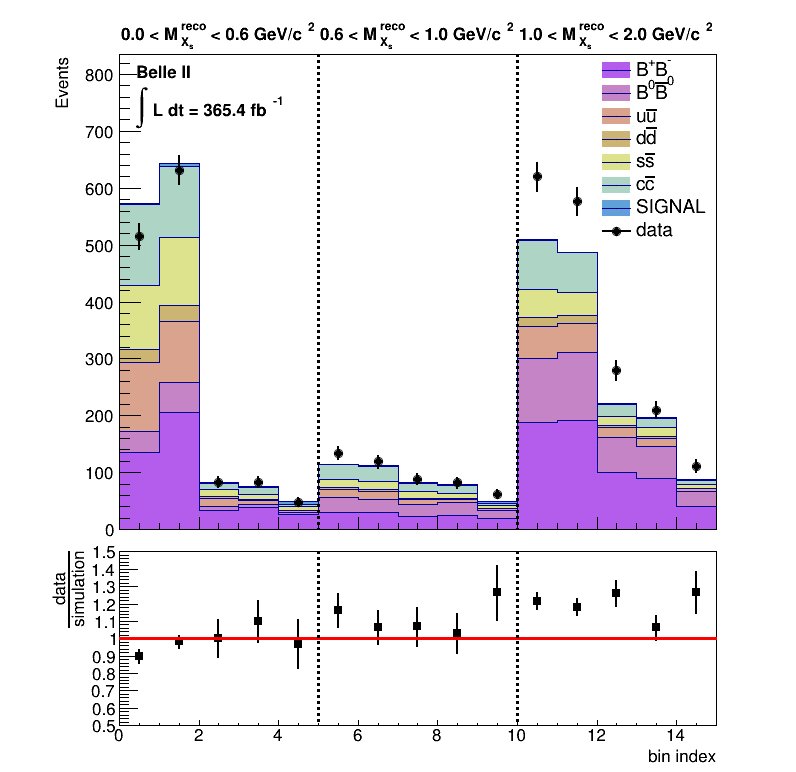
\includegraphics[width=0.5\textwidth]{./picture/unblind/prefit.png}}
  \caption{The bin-index distribution before the fit.}
  \label{fig:bin_index_prefit}
\end{figure}
The chi squared value for this distribution is
\begin{equation*}
    \chi^{2}_{15} = 54.3,
\end{equation*}
where the number of degrees of freedom is 15 because there are 15 bins.
The p-value for this chi squared value is
\begin{equation}
    \textrm{p-value} = \mathcal{P}(\chi^{2}_{15} > 54.3) < 0.01.
\end{equation}
This low p-value mainly originates from the $0.6 < M_{X_{s}}^{\textrm{reco}} < 2.0~\textrm{GeV}$ region, as shown in Figure~\ref{fig:bin_index_prefit}.

Figure~\ref{fig:bin_index_postfit} shows the bin-index distribution after the fit.
\begin{figure}
  \centering
  \subfloat{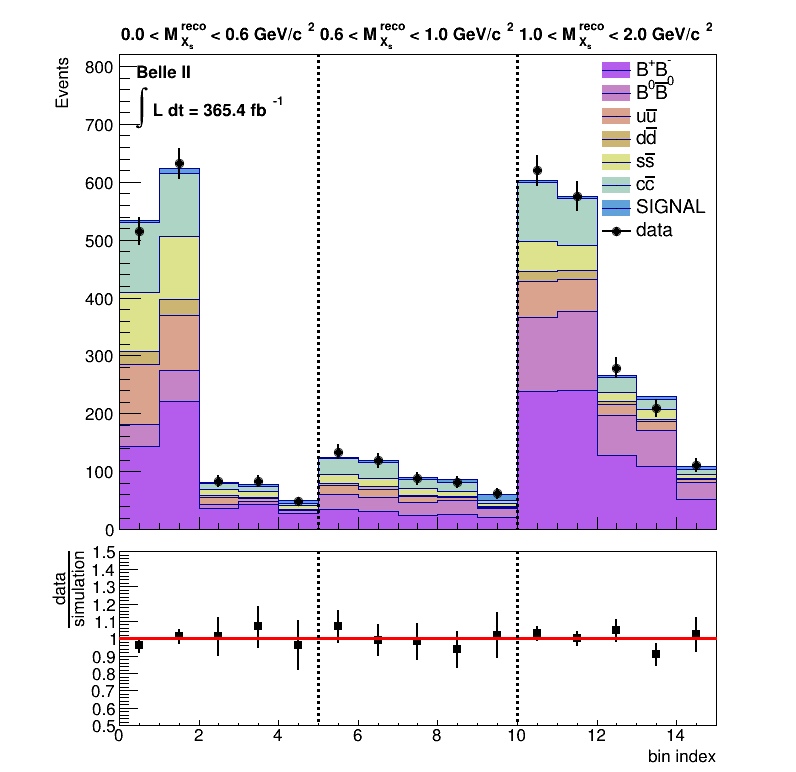
\includegraphics[width=0.5\textwidth]{./picture/unblind/postfit.png}}
  \caption{The bin-index distribution after the fit. The three signal strengths are set as free parameters.}
  \label{fig:bin_index_postfit}
\end{figure}
The chi squared value for this distribution is
\begin{equation}
    \chi^{2}_{12} = 5.4,
\end{equation}
where the number of degrees of freedom is 12 because three free parameters are used for 15 bins.
The p-value for this chi squared value is
\begin{equation}
    \textrm{p-value} = \mathcal{P}(\chi^{2}_{12} > 5.4) = 0.94.
\end{equation}
The fit result is
\begin{equation}
    \label{eq:fit_result_three_mu}
    \mu = 
  \begin{cases}
    0.5^{+1.7}_{-1.6}(\textrm{stat})^{+1.7}_{-1.4}(\textrm{syst})=0.5^{+2.4}_{-2.1} & (0.0 < M_{X_{s}} < 0.6~\textrm{GeV}/c^{2}), \\[10pt]
    4.1^{+3.1}_{-3.0}(\textrm{stat})^{+3.6}_{-3.0}(\textrm{syst})=4.1^{+4.8}_{-4.2} & (0.6 < M_{X_{s}} < 1.0~\textrm{GeV}/c^{2}), \\[10pt]
    3.2^{+5.9}_{-5.6}(\textrm{stat})^{+8.1}_{-7.0}(\textrm{syst})=3.2^{+10.0}_{-9.0} & (1.0~\textrm{GeV}/c^{2} < M_{X_{s}}), \\
  \end{cases}
\end{equation}
where the fitter bias is not considered.

However, as discussed in Section~\ref{sec:fit_quality}, a bias associated with the fitter is observed.
To include this effect as a post-unblinding systematic uncertainty, a toy MC study is performed.
A total of 10000 toy MC samples are generated with the $\mu$ values obtained in Eq.~\ref{eq:fit_result_three_mu}.
The nuisance parameters are varied according to Gaussian distributions.
The pull value is then calculated using Eq.~\ref{eq:pull_equation}.
The systematic uncertainty from the fitter bias is calculated as follows:
\begin{align}
    \sigma_{\textrm{syst mean}} =& \sigma_{\textrm{total}} \times \mu_{\textrm{pull}},\\
    \sigma_{\textrm{syst width}} =& \sigma_{\textrm{total}} \times (\sigma_{\textrm{pull}} - 1),
\end{align}
where $\sigma_{\textrm{syst mean}}$ is the systematic uncertainty from the mean of the pull distribution, $\mu_{\textrm{pull}}$ is the mean of the pull distribution, $\sigma_{\textrm{syst width}}$ is the systematic uncertainty from the width of the pull distribution, $\sigma_{\textrm{pull}}$ is the width of the pull distribution, and $\sigma_{\textrm{total}}$ is the total uncertainty from the fit.
Here, $\sigma_{\textrm{total}}$ is obtained from the fit result.

After including this systematic uncertainty, the fit result is
\begin{equation}
    \mu = 
  \begin{cases}
    0.5^{+1.7}_{-1.6}(\textrm{stat})^{+1.7}_{-1.5}(\textrm{syst})=0.5^{+2.4}_{-2.1} & (0.0 < M_{X_{s}} < 0.6~\textrm{GeV}/c^{2}), \\[10pt]
    4.1^{+3.1}_{-3.0}(\textrm{stat})^{+3.6}_{-3.0}(\textrm{syst})=4.1^{+4.8}_{-4.2} & (0.6 < M_{X_{s}} < 1.0~\textrm{GeV}/c^{2}), \\[10pt]
    3.2^{+5.9}_{-5.6}(\textrm{stat})^{+8.3}_{-7.0}(\textrm{syst})=4.6^{+10.1}_{-9.0} & (1.0~\textrm{GeV}/c^{2} < M_{X_{s}}), \\
\end{cases}
\end{equation}
When converted into branching ratios, the results become
\begin{equation}
    BR(B\rightarrow X_{s} \nu \bar{\nu}) = 
  \begin{cases}
    [0.3^{+0.8}_{-0.8}(\textrm{stat})^{+0.8}_{-0.7}(\textrm{syst})]\times 10^{-5} & (0.0 < M_{X_{s}} < 0.6~\textrm{GeV}/c^{2}), \\[10pt]
    [3.5^{+2.7}_{-2.5}(\textrm{stat})^{+3.1}_{-2.6}(\textrm{syst})]\times 10^{-5} & (0.6 < M_{X_{s}} < 1.0~\textrm{GeV}/c^{2}), \\[10pt]
    [5.1^{+9.2}_{-8.8}(\textrm{stat})^{+12.9}_{-11.0}(\textrm{syst})]\times 10^{-5} & (1.0~\textrm{GeV}/c^{2} < M_{X_{s}}).
  \end{cases}
\end{equation}

When the three mass regions are combined, the signal strength and branching ratio are obtained as
\begin{equation}
    \mu = 3.0^{+2.9}_{-2.8}(\textrm{stat})^{+4.4}_{-3.7}(\textrm{syst})=3.0^{+5.2}_{-4.7},
\end{equation}
and
\begin{equation}
    BR(B\rightarrow X_{s} \nu \bar{\nu}) = [8.8^{+8.5}_{-8.2}(\textrm{stat})^{+12.6}_{-10.7}(\textrm{syst})]\times 10^{-5}.
\end{equation}

Table~\ref{tab:uncertaintiestable_data} shows the impact of each systematic uncertainty on $\sigma_{\mu}$.
These values are determined using Eq.~\ref{eq:syst_break}.
\begin{table}
\caption{Summary of the systematic and statistical uncertainties for the three signal-strength parameters. The values are obtained from data.}
  \renewcommand{\arraystretch}{1.4}
  \centering
\begin{tabular}{ p{6cm} p{2.5cm} p{2.5cm} p{2.5cm}}
 \hline
  \hline
Source & Impact on $\sigma_{\mu_{1}}$ & Impact on $\sigma_{\mu_{2}}$ & Impact on $\sigma_{\mu_{3}}$\\
 \hline
Background normalization & 1.17 & 2.34 & 4.19 \\
MC statistics & 0.90 & 1.78 & 4.04 \\
FastBDT efficiency & 0.10 & 0.49 & 1.44 \\
$K^{*}-X_{s}$ transition & 0.01 & 0.04 & 1.40 \\
BR of main $B$ meson decays & 0.25 & 0.72 & 1.30 \\
$q\bar{q}$ efficiency & 0.19 & 0.25 & 1.16 \\
Fitter bias & 0.31 & 0.07 & 1.08 \\
Photon multiplicity correction & 0.05 & 0.29 & 1.02 \\
Additional FEI calibration factor & 0.17 & 0.46 & 0.63 \\
FEI calibration for $B\bar{B}$ & 0.15 & 0.33 & 0.51 \\
Fragmentation & 0.02 & 0.08 & 0.46 \\
$q\bar{q}$ shape & 0.22 & 0.27 & 0.46 \\
Fermi motion momentum & 0.00 & 0.00 & 0.44 \\
$B\Bbar$ counting & 0.04 & 0.16 & 0.38 \\
$B\rightarrow K^{*}$ form factor & 0.03 & 0.59 & 0.36 \\
BR of $B \rightarrow X_{s} K_{L}^{0} K_{L}^{0}$ & 0.01 & 0.39 & 0.35 \\
Fraction of decay modes & 0.13 & 0.32 & 0.28 \\
$b$-quark mass & 0.00 & 0.00 & 0.22 \\
BR of $B\rightarrow X_{s} n\bar{n}$ decay & 0.13 & 0.49 & 0.16 \\
$B\rightarrow K$ form factor & 0.13 & 0.00 & 0.16 \\
Pion ID & 0.01 & 0.09 & 0.15 \\
BR of $D \rightarrow K_{L}^{0} X$ from B meson & 0.01 & 0.11 & 0.12 \\
Tracking efficiency & 0.01 & 0.03 & 0.10 \\
$\pi^{0}$ reconstruction & 0.01 & 0.04 & 0.09 \\
$K_{S}^{0}$ reconstruction & 0.02 & 0.04 & 0.05 \\
$K_{L}^{0}$ ECL efficiency & 0.01 & 0.02 & 0.05 \\
Kaon ID & 0.06 & 0.02 & 0.04 \\
\hline
Statistical uncertainty & 1.62 & 3.04 & 5.75 \\
         \hline
            \hline
\end{tabular}
    \label{tab:uncertaintiestable_data}
\end{table}
Table~\ref{tab:uncertaintiestable_data_BR} shows the impact on the branching ratios for each systematic uncertainty.

Because no evidence for a signal is observed, upper limits are calculated.
For each $M_{X_{s}}$ region, the upper limits are
\begin{equation}
    UL(\mu) = 
  \begin{cases}
    4.5 & (0.0 < M_{X_{s}} < 0.6~\textrm{GeV}/c^{2}), \\[10pt]
    11.0 & (0.6 < M_{X_{s}} < 1.0~\textrm{GeV}/c^{2}), \\[10pt]
    19.7 & (1.0~\textrm{GeV}/c^{2} < M_{X_{s}}), 
  \end{cases}
\end{equation}
at the 90\% confidence level, including the fitter-bias systematic uncertainty.
When converted into branching-ratio upper limits, these become
\begin{equation}
    UL(B\rightarrow X_{s} \nu \bar{\nu}) = 
  \begin{cases}
    2.2\times 10^{-5} & (0.0 < M_{X_{s}} < 0.6~\textrm{GeV}/c^{2}), \\[10pt]
    9.3\times 10^{-5} & (0.6 < M_{X_{s}} < 1.0~\textrm{GeV}/c^{2}), \\[10pt]
    30.9\times 10^{-5} & (1.0~\textrm{GeV}/c^{2} < M_{X_{s}}), 
  \end{cases}
\end{equation}
When the three mass regions are combined, the upper limits are
\begin{equation}
    UL(\mu) = 
    11.3,
\end{equation}
and
\begin{equation}
    \label{eq:upper_limit}
    UL(B\rightarrow X_{s} \nu \bar{\nu}) = 
    32.7 \times 10^{-5},
\end{equation}
at the 90\% confidence level, including the fitter-bias systematic uncertainty.
Figure~\ref{fig:CLs_unblind} shows the results of the $CL_{s}$ method.
\begin{figure}
    \centering
    \subfloat[][$0.0 < M_{X_{s}} < 0.6~\textrm{GeV}/c^{2}$]
    {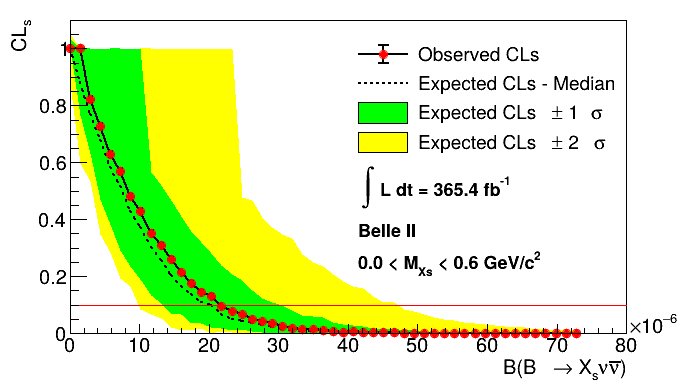
\includegraphics[width=0.47\textwidth]{./picture/unblind/UL_MXs1.png}}
    \subfloat[][$0.6 < M_{X_{s}} < 1.0~\textrm{GeV}/c^{2}$]
    {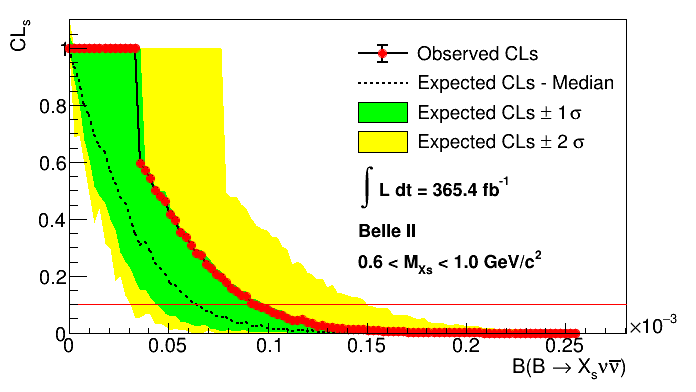
\includegraphics[width=0.47\textwidth]{./picture/unblind/UL_MXs2.png}}\\
    \subfloat[][$1.0~\textrm{GeV}/c^{2} < M_{X_{s}}$]
    {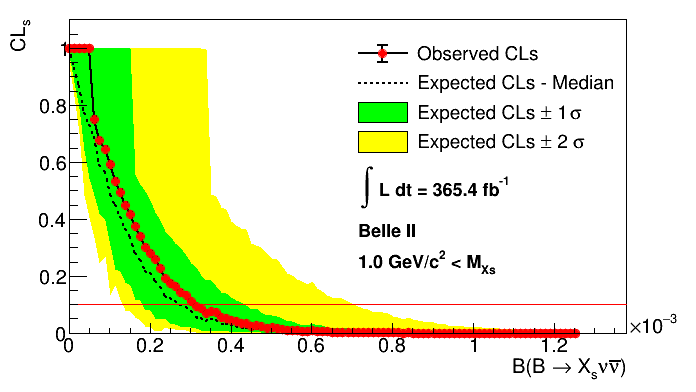
\includegraphics[width=0.47\textwidth]{./picture/unblind/UL_MXs3.png}}
    \subfloat[][Full $M_{X_{s}}$ range]
    {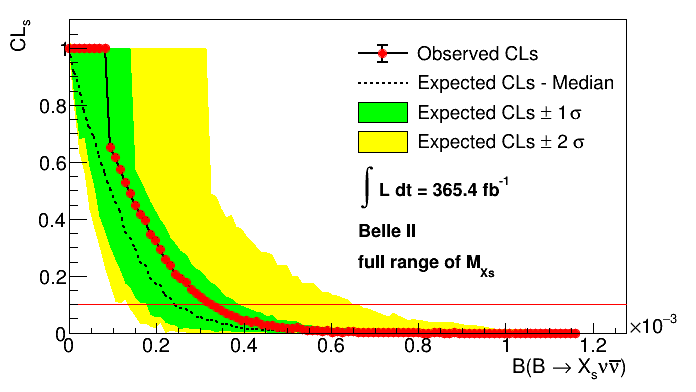
\includegraphics[width=0.47\textwidth]{./picture/unblind/UL_mu_sum.png}}
    \caption{$CL_{s}$ values as functions of the tested branching ratio,
    obtained using data.}
    \label{fig:CLs_unblind}
\end{figure}

\begin{table}
\caption{Summary of the systematic and statistical uncertainties in the full range and in each mass region. The values are obtained from data.}
\renewcommand{\arraystretch}{1.3}
\setlength{\tabcolsep}{3pt}
\centering
\small

\begin{tabularx}{\textwidth}{
    >{\raggedright\arraybackslash}X
    >{\centering\arraybackslash}p{1.9cm}
    >{\centering\arraybackslash}p{1.6cm}
    >{\centering\arraybackslash}p{1.6cm}
    >{\centering\arraybackslash}p{2.4cm}
}
 \hline
 \hline
&
\multicolumn{4}{c}{
    Impact on $\sigma_{BR}$ [$10^{-5}$] in $M_{X_s}^{\textrm{reco}}$ regions [$\textrm{GeV}/c^{2}$]
} \\
\cline{2-5}
Source
& Full range
& $[0, 0.6]$
& $[0.6, 1.0]$
& $[1.0, M_{X_s}^{\textrm{max}}]$ \\
\hline
MC statistics & 6.0 & 0.4 & 1.5 & 6.3 \\
Background normalization & 5.7 & 0.6 & 2.0 & 6.6 \\
BR of main $B$ meson decays& 2.3 & 0.1 & 0.6 & 2.0 \\
$K^{*}-X_{s}$ transition & 2.1 & 0.0 & 0.0 & 2.2 \\
FastBDT efficiency & 2.1 & 0.0 & 0.4 & 2.3 \\
Photon multiplicity correction & 1.8 & 0.0 & 0.2 & 1.6 \\
$q\bar{q}$ efficiency & 1.8 & 0.1 & 0.2 & 1.8 \\
Fitter bias & 1.6 & 0.2 & 0.1 & 1.7 \\
FEI calibration for $B\bar{B}$ & 1.1 & 0.1 & 0.3 & 0.8 \\
Additional FEI calibration factor & 1.0 & 0.1 & 0.4 & 1.0 \\
$q\bar{q}$ shape & 1.0 & 0.1 & 0.2 & 0.7 \\
BR of $B \rightarrow X_{s} K_{L}^{0} K_{L}^{0}$ & 0.9 & 0.0 & 0.3 & 0.6 \\
$B\Bbar$ counting & 0.7 & 0.0 & 0.1 & 0.6 \\
Fermi motion momentum & 0.7 & 0.0 & 0.0 & 0.7 \\
Fragmentation & 0.6 & 0.0 & 0.1 & 0.7 \\
$B\rightarrow K^{*}$ form factor & 0.6 & 0.0 & 0.5 & 0.6 \\
BR of $B\rightarrow X_{s} n\bar{n}$ decay & 0.5 & 0.1 & 0.4 & 0.2 \\
Fraction of decay modes & 0.4 & 0.1 & 0.3 & 0.4 \\
$b$-quark mass & 0.3 & 0.0 & 0.0 & 0.3 \\
BR of $D \rightarrow K_{L}^{0} X$ from B meson & 0.3 & 0.0 & 0.1 & 0.2 \\
Pion ID & 0.2 & 0.0 & 0.1 & 0.2 \\
$B\rightarrow K$ form factor & 0.2 & 0.1 & 0.0 & 0.2 \\
Tracking efficiency & 0.2 & 0.0 & 0.0 & 0.1 \\
$\pi^{0}$ reconstruction & 0.1 & 0.0 & 0.0 & 0.1 \\
Kaon ID & 0.1 & 0.0 & 0.0 & 0.1 \\
$K_{S}^{0}$ reconstruction & 0.1 & 0.0 & 0.0 & 0.1 \\
$K_{L}^{0}$ ECL efficiency & 0.1 & 0.0 & 0.0 & 0.1 \\
\hline
Total systematic sources & 11.7 & 0.8 & 2.8 & 12.0 \\
\hline
Statistical uncertainty & 8.3 & 0.8 & 2.6 & 9.0 \\

 \hline
 \hline
\end{tabularx}
    \label{tab:uncertaintiestable_data_BR}
\end{table}

\chapter{Discussion}

\section{Constraints on new physics}

\subsection{Model-independent constraint}

Using the Wilson coefficients $C^{\nu}_{L,R}$, two observables can be
defined~\cite{Altmannshofer:2009ma}:
\begin{linenomath*}
  \begin{align}
    \epsilon &=
    \frac{\sqrt{\left| C_{L}^{\nu} \right|^{2}
    + \left| C_{R}^{\nu} \right|^{2}}}
    {\left|(C_{L}^{\nu})^{\textrm{SM}} \right|},\\
    \eta &=
    \frac{-\textrm{Re}(C_{L}^{\nu}C_{R}^{\nu*})}
    {\left| C_{L}^{\nu} \right|^{2}
    + \left| C_{R}^{\nu} \right|^{2}}.
  \end{align}
\end{linenomath*}
In terms of these two observables, the branching ratio of
$B \rightarrow X_{s} \nu \bar{\nu}$ decays is given by
~\cite{Altmannshofer:2009ma}
\begin{equation}
    BR(B\rightarrow X_{s} \nu \bar{\nu})
    =
    BR(B\rightarrow X_{s} \nu \bar{\nu})_{\textrm{SM}}
    \times (1+0.09\eta)\epsilon^{2}.
\end{equation}
Using the upper limit in Eq.~\ref{eq:upper_limit}, an allowed region can be
defined at the 90\% confidence level:
\begin{equation}
    BR(B\rightarrow X_{s} \nu \bar{\nu})_{\textrm{SM}}
    \times (1+0.09\eta)\epsilon^{2}
    <
    UL(B\rightarrow X_{s} \nu \bar{\nu}).
\end{equation}
Figure~\ref{fig:model_indep} shows the allowed region in the
$\epsilon$--$\eta$ plane.
\begin{figure}
  \centering
  \subfloat{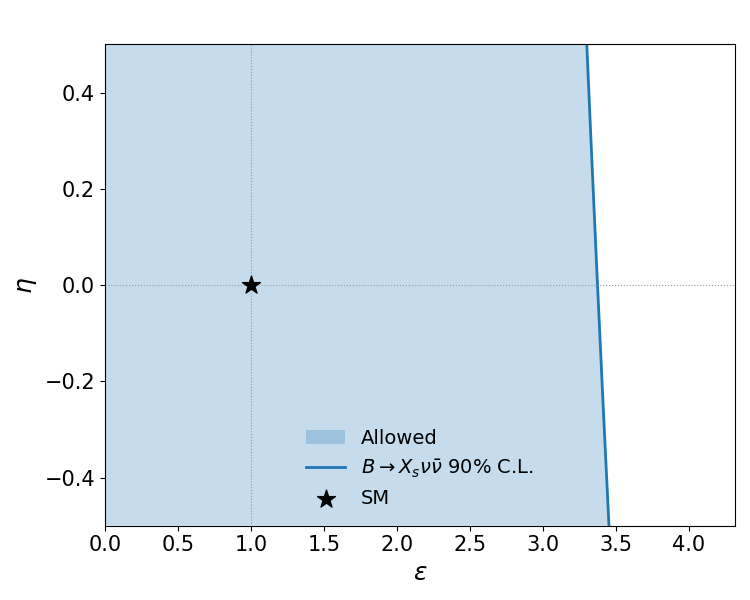
\includegraphics[width=0.6\textwidth]{./picture/discussion/model_indep_plot.png}}
  \caption{Allowed region in the $\epsilon$--$\eta$ plane.}
  \label{fig:model_indep}
\end{figure}

\subsection{Flavour-violating $\bar{b}sZ'$ coupling}

As discussed in Section~\ref{sec:Zprime_model}, a flavour-violating
$\bar{b}sZ'$ coupling is considered.
The ratio of the branching ratios in the presence and absence of this
coupling is given by~\cite{Altmannshofer:2009ma}
\begin{equation}
    \frac{BR(B\rightarrow X_{s} \nu \bar{\nu})}
    {BR(B\rightarrow X_{s} \nu \bar{\nu})_{\textrm{SM}}}
    =
    \frac{|C_{L}^{\nu}|^{2}+|C_{R}^{\nu}|^{2}
    -0.09\textrm{Re}(C_{L}^{\nu}C_{R}^{\nu*})}
    {|(C_{L}^{\nu})_{\textrm{SM}}|^{2}},
\end{equation}
where $(C_{L}^{\nu})_{\textrm{SM}}=-6.38$.
Substituting Eq.~\ref{eq:Zprime_wilson_Xsnunubar} gives
\begin{equation}
    \frac{BR(B\rightarrow X_{s} \nu \bar{\nu})}
    {BR(B\rightarrow X_{s} \nu \bar{\nu})_{\textrm{SM}}}
    =
    \frac{|6.38+\frac{Z'_{L}}{2}|^{2}
    +|\frac{Z'_{R}}{2}|^{2}
    -0.09((6.38+\frac{Z'_{L}}{2})\times\frac{Z'_{R}}{2})}
    {6.38^{2}}.
\end{equation}
As a benchmark scenario, $Z'_{L}$ and $Z'_{R}$ are assumed to be real,
and the vector coupling of the $Z'$ to neutrinos is fixed to
$g'^{\nu}_{V}=1$.
Using the upper limit in Eq.~\ref{eq:upper_limit}, an allowed region can be
defined at the 90\% confidence level:
\begin{equation}
    BR(B\rightarrow X_{s} \nu \bar{\nu})_{\textrm{SM}}
    \times
    \frac{|6.38+\frac{Z'_{L}}{2}|^{2}
    +|\frac{Z'_{R}}{2}|^{2}
    -0.09((6.38+\frac{Z'_{L}}{2})\times\frac{Z'_{R}}{2})}
    {6.38^{2}}
    <
    UL(B\rightarrow X_{s} \nu \bar{\nu}).
\end{equation}
Figure~\ref{fig:model_Zprime} shows the allowed region in the
$Z'_{L}$--$Z'_{R}$ plane.
\begin{figure}
  \centering
  \subfloat{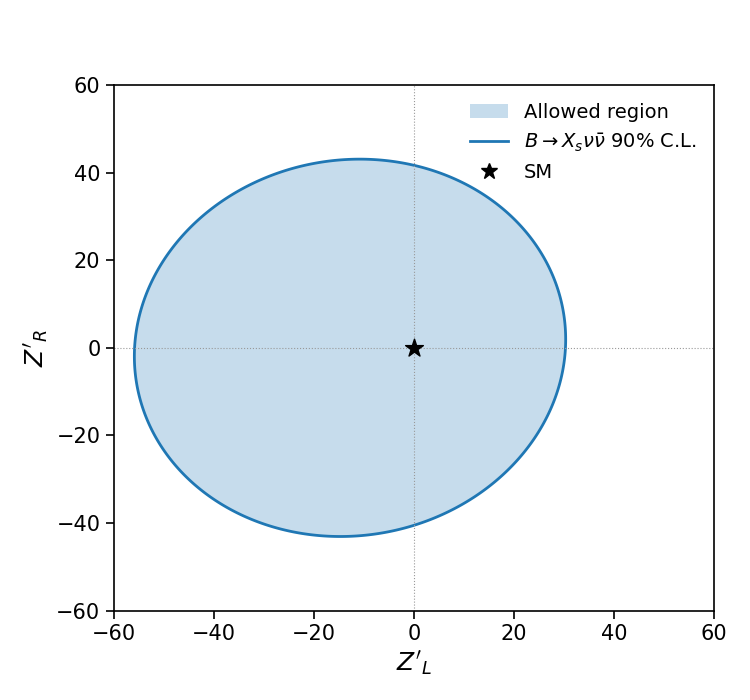
\includegraphics[width=0.6\textwidth]{./picture/discussion/model_Zprime.png}}
  \caption{
  Allowed region in the $Z'_{L}$--$Z'_{R}$ plane.
  As a benchmark scenario, $Z'_{L}$ and $Z'_{R}$ are assumed to be real,
  and the vector coupling of the $Z'$ to neutrinos is fixed to
  $g'^{\nu}_{V}=1$.
  }
  \label{fig:model_Zprime}
\end{figure}

\subsection{Invisible light scalar}

As discussed in Section~\ref{sec:invisible_scalar}, an invisible light
scalar is considered.
Using Eq.~\ref{eq:lagrangian_light_scalar}, the differential decay width
for the process involving this invisible particle is given by
~\cite{Calcuttawala:2017usw}
\begin{equation}
\label{eq:partial_dw_invisible_scalar}
\begin{aligned}
\frac{d\Gamma(B \rightarrow X_s SS)}{dq^2}
={}&
\frac{|C_{S1}|^2 + |C_{S2}|^2}
     {128\pi^3 m_b \Lambda^4}
\sqrt{1-\frac{4m_S^2}{q^2}}\,
\lambda^{1/2}(m_b^2,m_s^2,q^2)
\\
&\times
\Bigg[
m_b^2+m_s^2-q^2
-4m_s m_b
\frac{\operatorname{Re}(C_{S1}C_{S2}^{*})}
     {|C_{S1}|^2+|C_{S2}|^2}
\Bigg].
\end{aligned}
\end{equation}
Here, $\Lambda$ denotes the new-physics scale, $m_{S}$ is the mass of the
invisible scalar $S$, and $q^{2}$ is the squared invariant mass of the
invisible system.
The branching ratio of $B \rightarrow X_{s}+\textrm{invisible}$ is then
given by
\begin{equation}
    \label{eq:BR_invisible}
    BR(B\rightarrow X_{s}+\textrm{invisible})
    =
    BR(B \rightarrow X_{s} \nu \bar{\nu})_{\textrm{SM}}
    +
    \frac{1}{\Gamma_{B}^{\textrm{tot}}}\int\frac{d\Gamma(B \rightarrow X_s SS)}{dq^2}dq^{2},
\end{equation}
where $\Gamma_{B}^{\textrm{tot}}$ denotes the total decay width of the $B$ meson.
As a benchmark scenario, $C_{S1}$ and $C_{S2}$ are assumed to be real.
Equation~\ref{eq:partial_dw_invisible_scalar} then becomes
\begin{equation}
\label{eq:partial_dw_invisible_scalar_real}
\begin{aligned}
\frac{d\Gamma(B \rightarrow X_s SS)}{dq^2}
={}&
\frac{
    \sqrt{1-4m_S^2/q^2}\,
    \lambda^{1/2}(m_b^2,m_s^2,q^2)
}{
    128\pi^3 m_b \Lambda^4
}
\\
&\times
\left[
    (C_{S1}^2+C_{S2}^2)
    (m_b^2+m_s^2-q^2)
    -4m_s m_b C_{S1}C_{S2}
\right].
\end{aligned}
\end{equation}
Using Eqs.~\ref{eq:BR_invisible}
and~\ref{eq:partial_dw_invisible_scalar_real}, together with the upper
limit in Eq.~\ref{eq:upper_limit}, an allowed two-dimensional region in
the $C_{S1}$--$C_{S2}$ plane can be derived.
Figure~\ref{fig:model_invisible} shows the allowed regions for several
values of $m_{S}$, assuming $\Lambda=1~\textrm{TeV}/c^{2}$ as a benchmark.
\begin{figure}
    \centering
    \subfloat[][$m_{S}=0.5~\textrm{GeV}/c^{2}$]
    {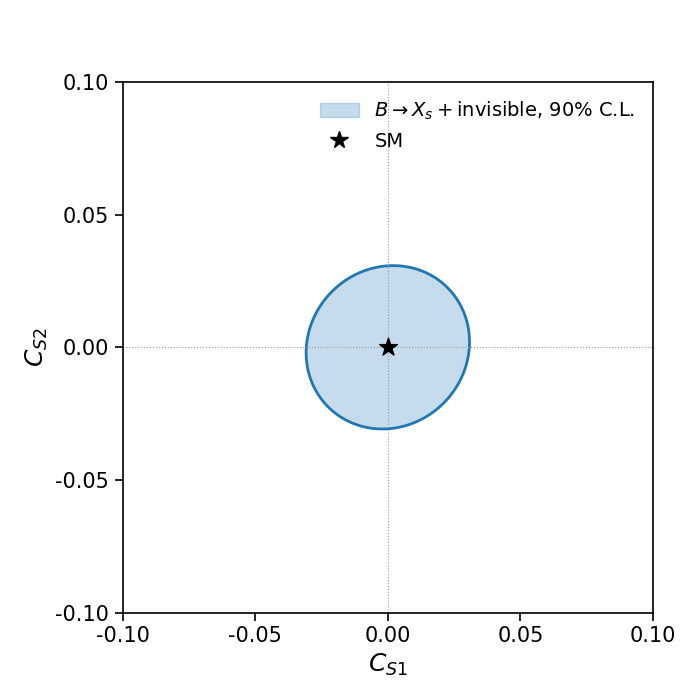
\includegraphics[width=0.47\textwidth]{./picture/discussion/CS1_CS2_Xs_constraint_05.png}}
    \subfloat[][$m_{S}=0.8~\textrm{GeV}/c^{2}$]
    {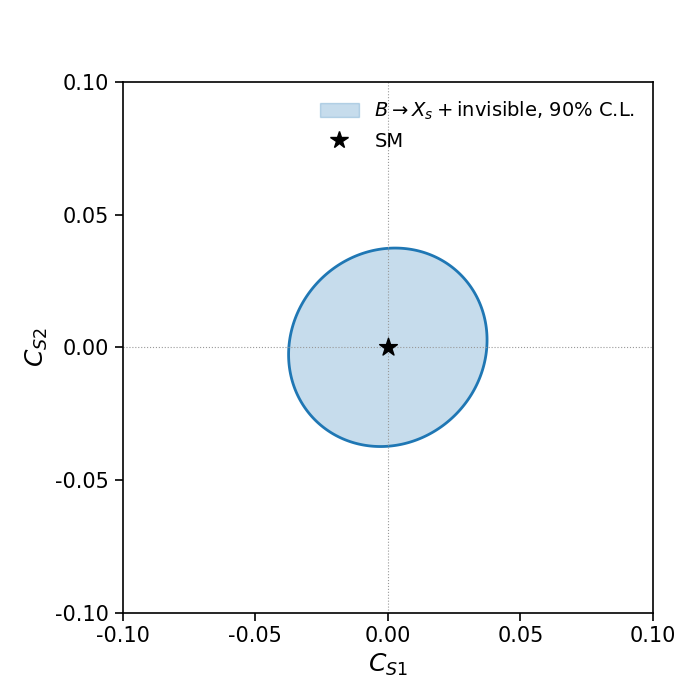
\includegraphics[width=0.47\textwidth]{./picture/discussion/CS1_CS2_Xs_constraint_08.png}}\\
    \subfloat[][$m_{S}=1.1~\textrm{GeV}/c^{2}$]
    {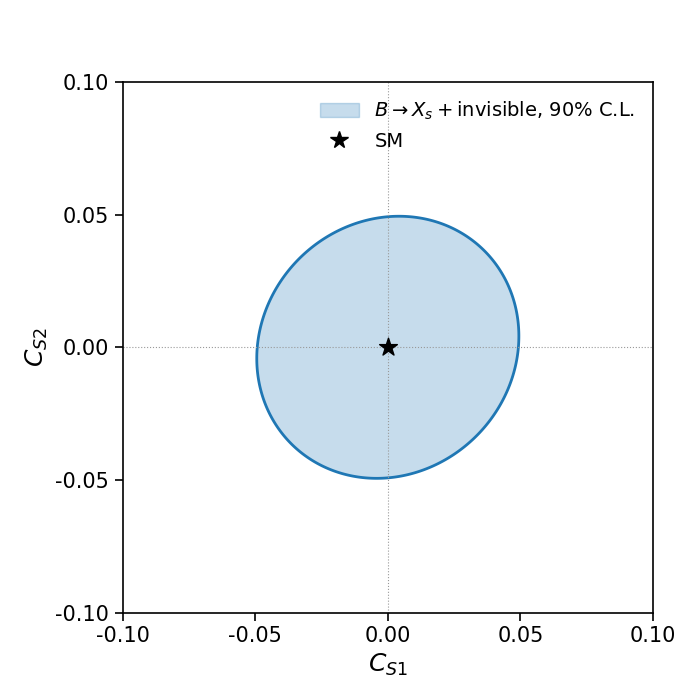
\includegraphics[width=0.47\textwidth]{./picture/discussion/CS1_CS2_Xs_constraint_11.png}}
    \subfloat[][$m_{S}=1.4~\textrm{GeV}/c^{2}$]
    {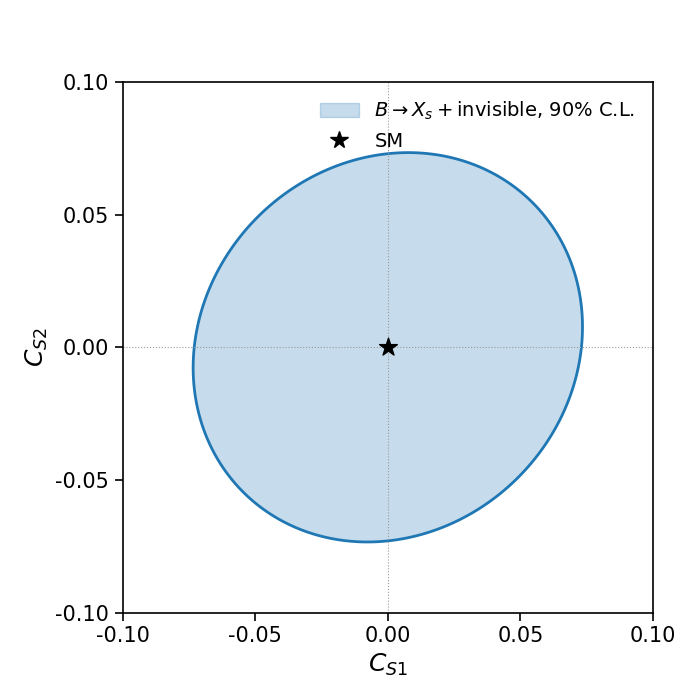
\includegraphics[width=0.47\textwidth]{./picture/discussion/CS1_CS2_Xs_constraint_14.png}}
    \caption{
    Allowed regions in the $C_{S1}$--$C_{S2}$ plane for several values of
    $m_{S}$.
    As a benchmark scenario, $C_{S1}$ and $C_{S2}$ are assumed to be real,
    and the new-physics scale is fixed to
    $\Lambda=1~\textrm{TeV}/c^{2}$.
    }
    \label{fig:model_invisible}
\end{figure}

\section{Prospects}
In this section, possible improvements to the analysis and the projected
sensitivity with a larger dataset are discussed.
The following improvements to the treatment of systematic uncertainties can
be implemented without additional data:
\begin{enumerate}
  \item \textbf{BR of main $B$ meson decays:}
  The branching ratios of the major $B$ meson decay modes are varied
  according to their uncertainties reported by the PDG.
  With dedicated studies, the relative uncertainties in
  $BR(B^{+}\rightarrow \bar{D}^{0} \pi^{+} \pi^{-} \pi^{+})$ and
  $BR(B^{+}\rightarrow \bar{D}^{0} \rho^{0} \pi^{+})$ may be reduced to
  10\%.

  \item \textbf{Background normalization:}
  A relative uncertainty of $\pm20\%$ is assigned to the background
  normalization.
  Instead, the correction factor and its uncertainty can be derived from
  the $M_{\textrm{bc}}$ and FastBDT sidebands.
  The correction factor can be taken as the average of the data-to-MC
  ratios in the two sidebands, and its uncertainty can be determined so as
  to cover the $1\sigma$ uncertainties of the data-to-MC ratios in both
  sidebands.
\end{enumerate}

With $50~\textrm{ab}^{-1}$ of data, the following additional improvements
can be implemented:
\begin{enumerate}
  \item \textbf{MC statistics:}
  The available MC samples are assumed to increase in proportion to the
  data luminosity, reducing the systematic uncertainty from finite MC
  statistics.

  \item \textbf{Pion ID, Kaon ID, Additional FEI calibration factor,
  $K_{S}^{0}$ reconstruction:}
  The statistical components of these uncertainties will be reduced.

  \item With larger data and MC samples, finer binning can be used in the
  fit.
  For example,
  [0.86, 0.9195, 0.979, 0.986, 0.9895, 0.993, 0.99475, 0.9965, 0.99825, 1.0],
  [0.86, 0.8925, 0.925, 0.95, 0.9625, 0.975, 0.98125, 0.9875, 0.99375, 1.0],
  and
  [0.86, 0.9, 0.94, 0.96, 0.97, 0.98, 0.985, 0.99, 0.995, 1.0]
  can be used for MR1, MR2, and MR3, respectively.

  \item Instead of using an $e^{+}e^{-}\rightarrow q\bar{q}$ template
  derived from MC, the off-resonance data can be used directly.
  This removes the systematic uncertainty associated with data--MC
  discrepancies in the continuum background.
\end{enumerate}

Table~\ref{tab:uncertaintiestable_50ab} shows the projected impact of each
systematic uncertainty for $50~\textrm{ab}^{-1}$ of data, incorporating
the improvements described above.

\begin{table}
\caption{Summary of the projected systematic and statistical uncertainties in the full range and in each mass region for $50~\textrm{ab}^{-1}$ of data.}
\renewcommand{\arraystretch}{1.3}
\setlength{\tabcolsep}{3pt}
\centering
\small

\begin{tabularx}{\textwidth}{
    >{\raggedright\arraybackslash}X
    >{\centering\arraybackslash}p{1.9cm}
    >{\centering\arraybackslash}p{1.6cm}
    >{\centering\arraybackslash}p{1.6cm}
    >{\centering\arraybackslash}p{2.4cm}
}
 \hline
 \hline
&
\multicolumn{4}{c}{
    Impact on $\sigma_{BR}$ [$10^{-5}$] in $M_{X_s}^{\textrm{reco}}$ regions [$\textrm{GeV}/c^{2}$]
} \\
\cline{2-5}
Source
& Full range
& $[0, 0.6]$
& $[0.6, 1.0]$
& $[1.0, M_{X_s}^{\textrm{max}}]$ \\
\hline
MC statistics & 0.9 & 0.1 & 0.2 & 0.8 \\
Background normalization & 0.2 & 0.1 & 0.2 & 0.3 \\
BR of main $B$ meson decays& 0.5 & 0.0 & 0.2 & 0.5 \\
$K^{*}-X_{s}$ transition & 0.3 & 0.0 & 0.0 & 0.4 \\
FastBDT efficiency & 0.3 & 0.0 & 0.1 & 0.3 \\
Photon multiplicity correction & 0.4 & 0.0 & 0.0 & 0.4 \\
Fitter bias & 0.3 & 0.1 & 0.0 & 0.3 \\
FEI calibration for $B\bar{B}$ & 0.3 & 0.1 & 0.1 & 0.3 \\
Additional FEI calibration factor & 0.1 & 0.1 & 0.1 & 0.1 \\
BR of $B \rightarrow X_{s} K_{L}^{0} K_{L}^{0}$ & 0.5 & 0.0 & 0.4 & 0.1 \\
$B\Bbar$ counting & 0.0 & 0.0 & 0.0 & 0.0 \\
Fermi motion momentum & 0.1 & 0.0 & 0.0 & 0.1 \\
Fragmentation & 0.0 & 0.0 & 0.0 & 0.0 \\
$B\rightarrow K^{*}$ form factor & 0.1 & 0.0 & 0.1 & 0.1 \\
BR of $B\rightarrow X_{s} n\bar{n}$ decay & 0.1 & 0.0 & 0.1 & 0.0 \\
Fraction of decay modes & 0.1 & 0.0 & 0.1 & 0.1 \\
$b$-quark mass & 0.1 & 0.0 & 0.0 & 0.1 \\
BR of $D \rightarrow K_{L}^{0} X$ from B meson & 0.0 & 0.0 & 0.0 & 0.0 \\
Pion ID & 0.5 & 0.0 & 0.1 & 0.4 \\
$B\rightarrow K$ form factor & 0.0 & 0.0 & 0.0 & 0.0 \\
Tracking efficiency & 0.0 & 0.0 & 0.0 & 0.0 \\
$\pi^{0}$ reconstruction & 0.7 & 0.0 & 0.1 & 0.7 \\
Kaon ID & 0.2 & 0.0 & 0.0 & 0.2 \\
$K_{S}^{0}$ reconstruction & 0.1 & 0.0 & 0.1 & 0.2 \\
$K_{L}^{0}$ ECL efficiency & 0.0 & 0.0 & 0.0 & 0.0 \\
\hline
Total systematic sources & 1.7 & 0.1 & 0.5 & 1.6 \\
\hline
Statistical uncertainty & 0.6 & 0.1 & 0.2 & 0.7 \\

 \hline
 \hline
\end{tabularx}
    \label{tab:uncertaintiestable_50ab}
\end{table}

Using the Asimov dataset with $\mu=1$, the expected upper limits are
\begin{equation}
    UL(B\rightarrow X_{s}\nu \bar{\nu}) =
  \begin{cases}
    0.72 \times 10^{-5} & (0.0 < M_{X_{s}} < 0.6~\textrm{GeV}/c^{2}), \\[10pt]
    1.67 \times 10^{-5} & (0.6 < M_{X_{s}} < 1.0~\textrm{GeV}/c^{2}), \\[10pt]
    4.54 \times 10^{-5} & (1.0~\textrm{GeV}/c^{2} < M_{X_{s}}).
  \end{cases}
\end{equation}
at the 90\% confidence level.

When the three mass regions are combined, the expected upper limit is
\begin{equation}
    UL(B\rightarrow X_{s}\nu \bar{\nu})
    = 5.53\times 10^{-5},
\end{equation}
at the 90\% confidence level.

Figure~\ref{fig:CLs_projection} shows the projected $CL_{s}$ results for $50~\textrm{ab}^{-1}$ of data.
\begin{figure}
    \centering
    \subfloat[][$0.0 < M_{X_{s}} < 0.6~\textrm{GeV}/c^{2}$]
    {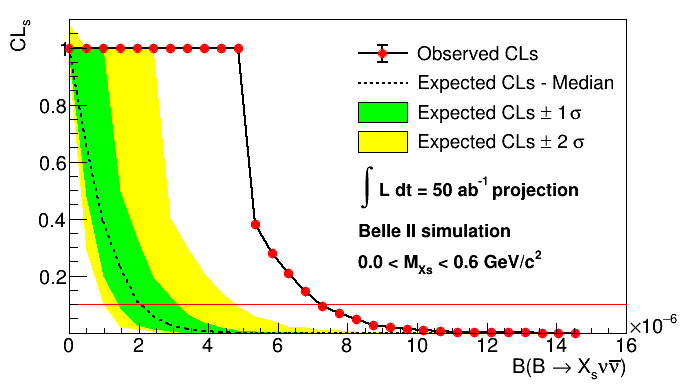
\includegraphics[width=0.47\textwidth]{./picture/projection/UL_MXs1.png}}
    \subfloat[][$0.6 < M_{X_{s}} < 1.0~\textrm{GeV}/c^{2}$]
    {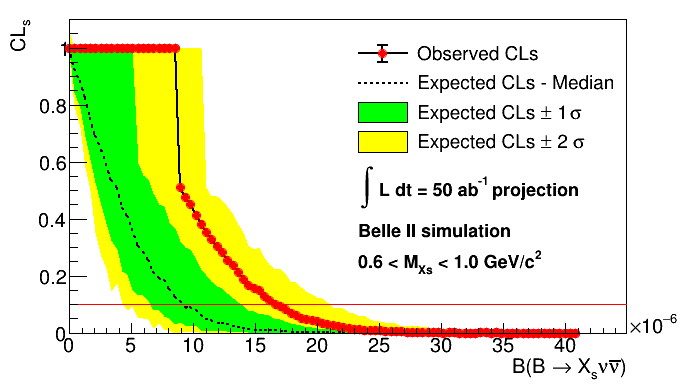
\includegraphics[width=0.47\textwidth]{./picture/projection/UL_MXs2.png}}\\
    \subfloat[][$1.0~\textrm{GeV}/c^{2} < M_{X_{s}}$]
    {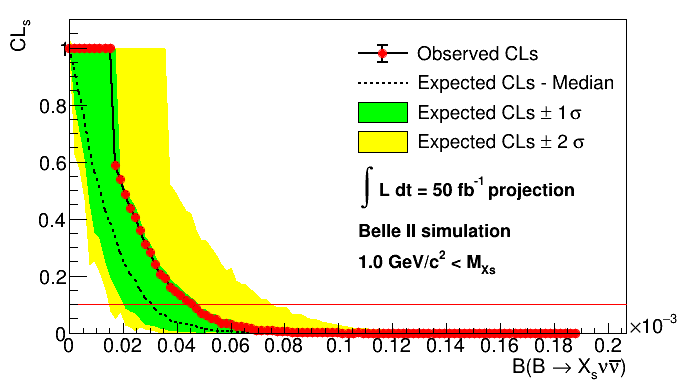
\includegraphics[width=0.47\textwidth]{./picture/projection/UL_MXs3.png}}
    \subfloat[][Full $M_{X_{s}}$ range]
    {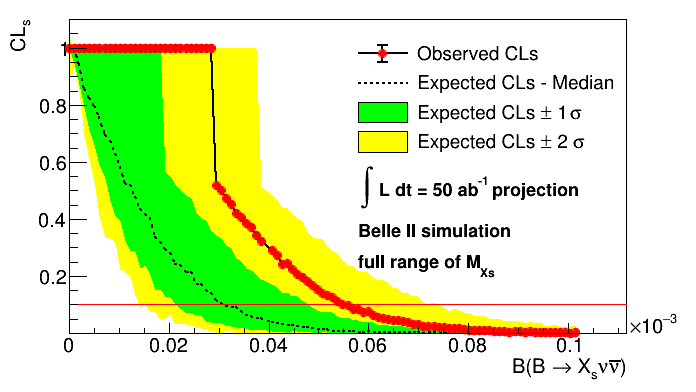
\includegraphics[width=0.47\textwidth]{./picture/projection/UL_mu_sum.png}}
    \caption{Projected $CL_{s}$ values as functions of the tested branching ratio for $50~\textrm{ab}^{-1}$ of data.}
    \label{fig:CLs_projection}
\end{figure}

\clearpage
\appendix

\chapter{Particle selection variable distributions}
\label{sec:particle_selection_distributions}
This appendix presents the distributions of the variables used for the particle selections described in Section~\ref{sec:particle_selection}, obtained from the signal MC sample.
MC truth information is used to distinguish correctly reconstructed (true) candidates from incorrectly reconstructed (fake) candidates.
For each distribution, the selection requirement on the plotted variable is omitted, while all other particle selection requirements are applied.

\begin{figure}[htbp]
    \centering
    \subfloat[][Invariant mass]{
        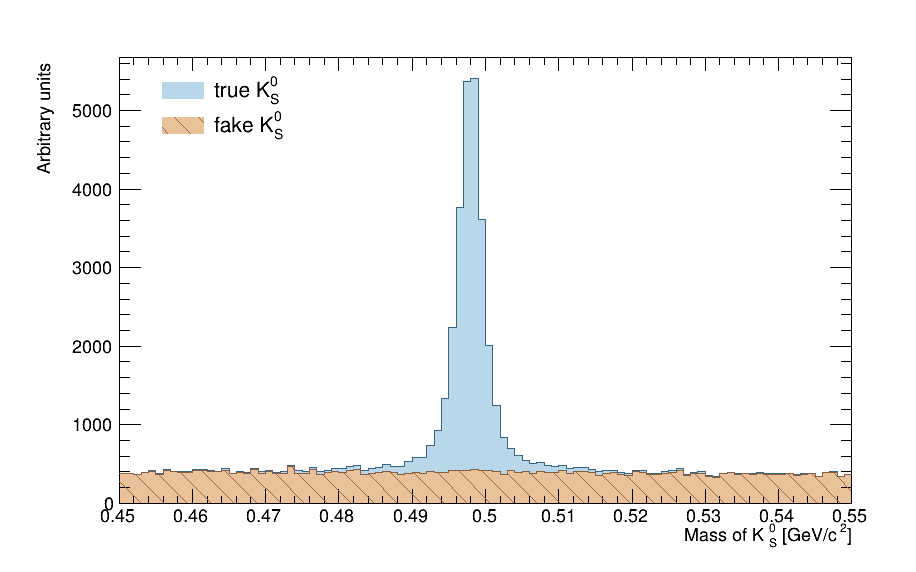
\includegraphics[width=0.47\textwidth]
        {./picture/particle_selections/08_KSzero_M_stack.png}
    }
    \hfill
    \subfloat[][\texttt{significanceOfDistance}]{
        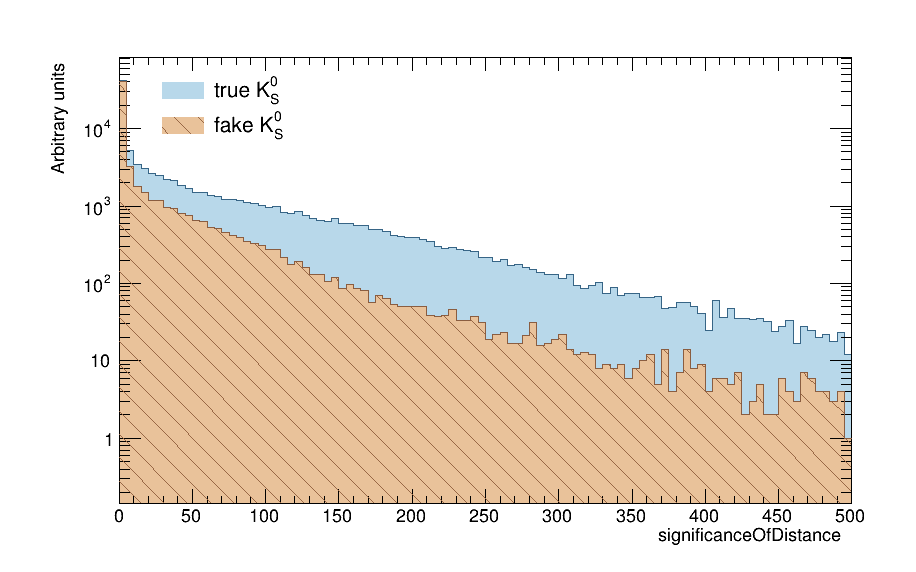
\includegraphics[width=0.47\textwidth]
        {./picture/particle_selections/09_KSzero_significanceOfDistance_stack.png}
    }
    \caption{
        Distributions of the variables used to select $K_S^0$
        candidates in the signal MC sample.
        The blue and orange hatched histograms represent true and
        fake candidates, respectively.
        In each panel, the selection requirement on the plotted variable
        is omitted, while all other particle selection requirements
        are applied.
    }
    \label{fig:particle_selection_ks}
\end{figure}

\begin{figure}[htbp]
    \centering
    \subfloat[][$dr$]{
        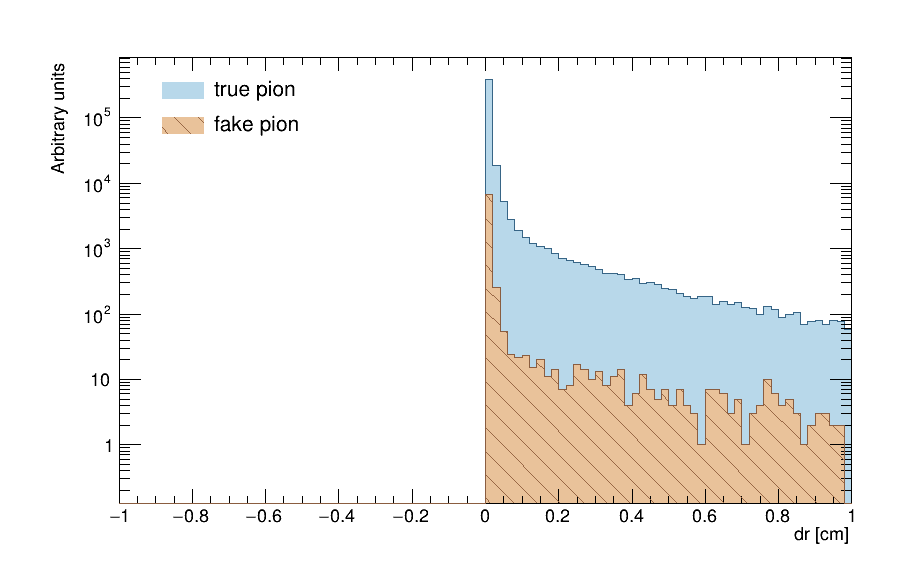
\includegraphics[width=0.47\textwidth]
        {./picture/particle_selections/10_pion_dr_stack.png}
    }
    \hfill
    \subfloat[][$dz$]{
        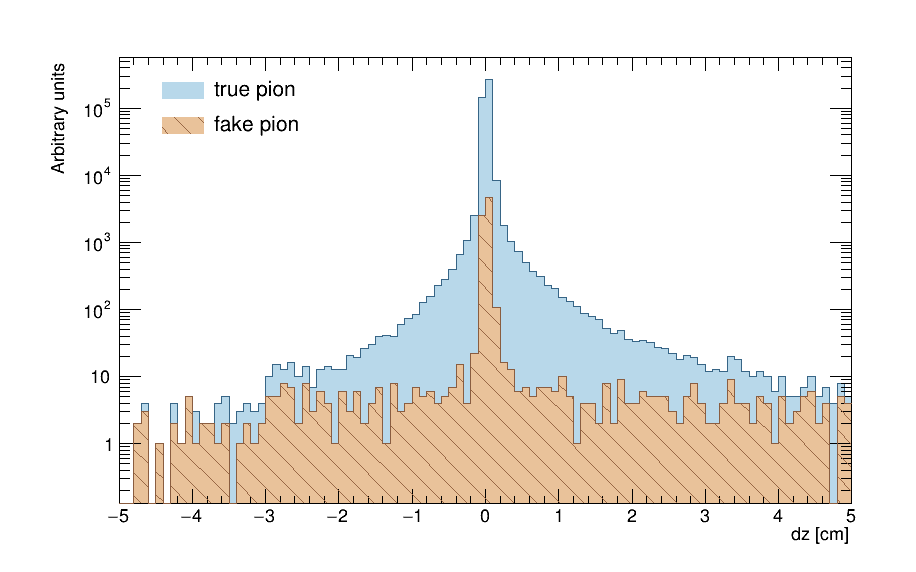
\includegraphics[width=0.47\textwidth]
        {./picture/particle_selections/11_pion_dz_stack.png}
    }\\
    \subfloat[][\texttt{nCDCHits}]{
        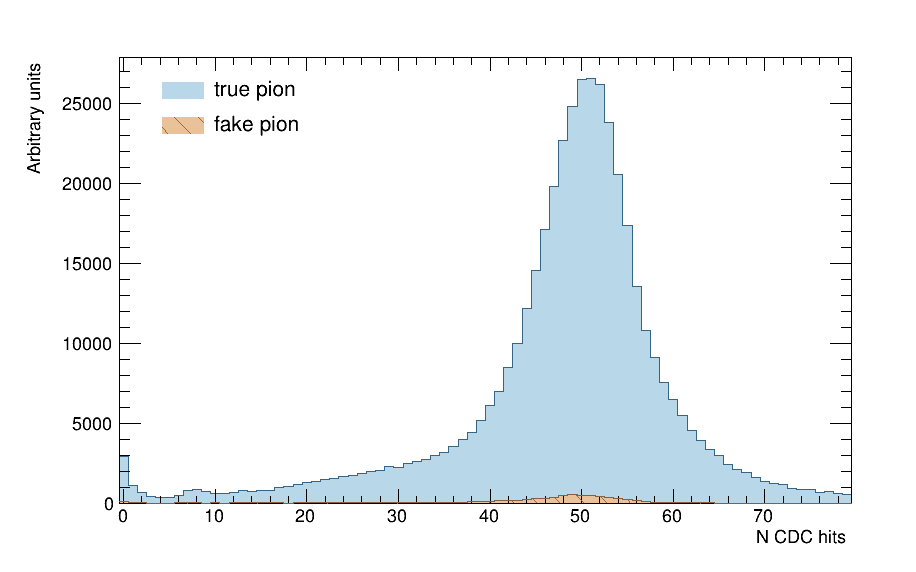
\includegraphics[width=0.47\textwidth]
        {./picture/particle_selections/12_pion_nCDCHits_stack.png}
    }
    \hfill
    \subfloat[][\texttt{nPXDHits}]{
        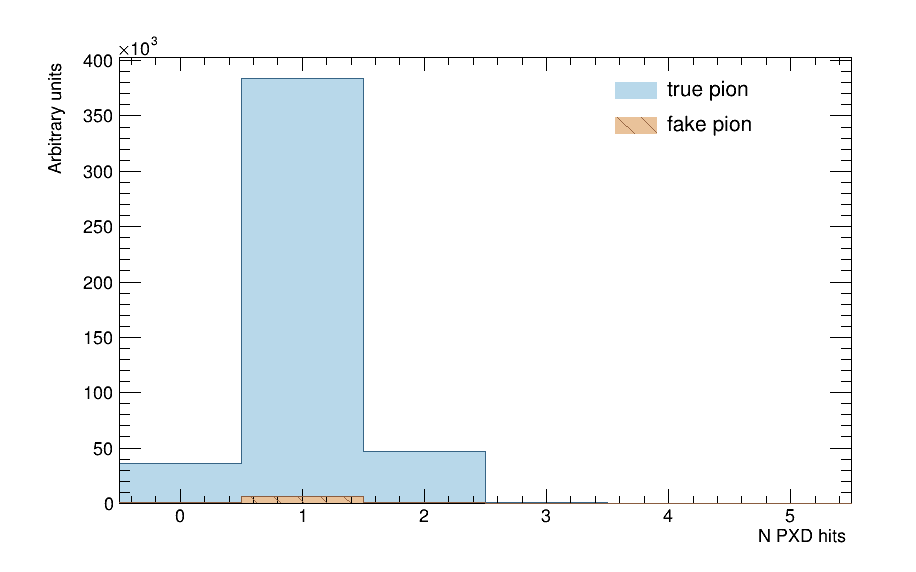
\includegraphics[width=0.47\textwidth]
        {./picture/particle_selections/13_pion_nPXDHits_stack.png}
    }\\
    \subfloat[][\texttt{pionID}]{
        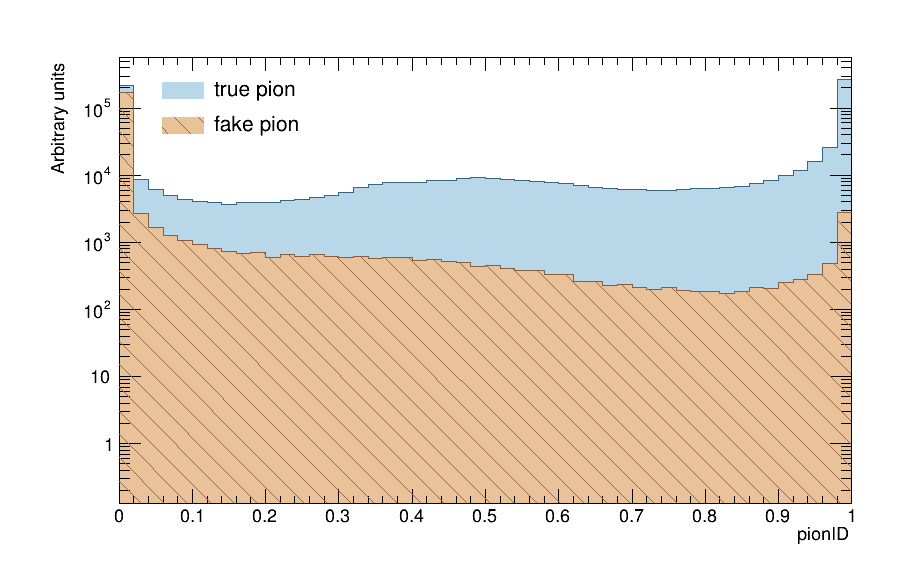
\includegraphics[width=0.47\textwidth]
        {./picture/particle_selections/14_pion_pionID_stack.png}
    }
    \caption{
        Distributions of the variables used to select charged pion
        candidates in the signal MC sample.
        The blue and orange hatched histograms represent true and
        fake candidates, respectively.
        In each panel, the selection requirement on the plotted variable
        is omitted, while all other particle selection requirements
        are applied.
    }
    \label{fig:particle_selection_pion}
\end{figure}

\begin{figure}[htbp]
    \centering
    \subfloat[][$dr$]{
        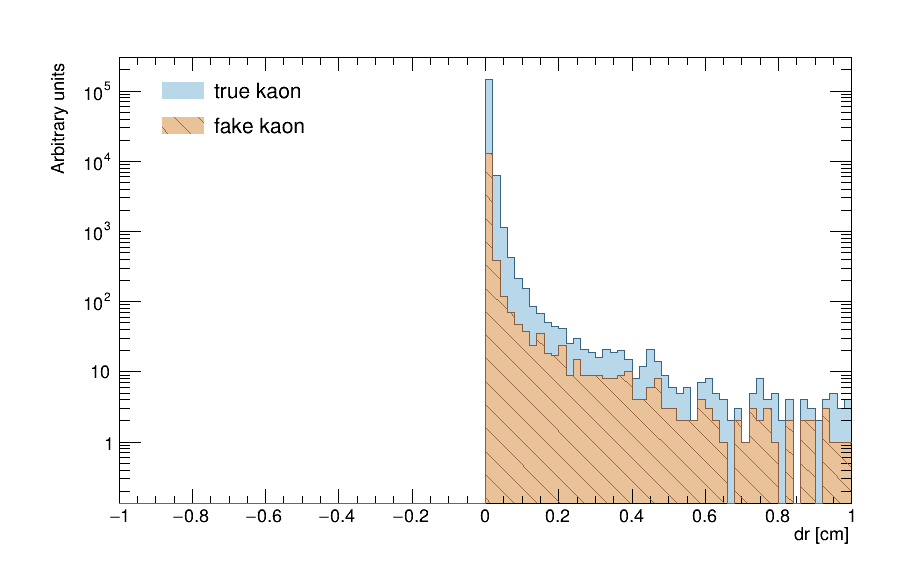
\includegraphics[width=0.47\textwidth]
        {./picture/particle_selections/15_kaon_dr_stack.png}
    }
    \hfill
    \subfloat[][$dz$]{
        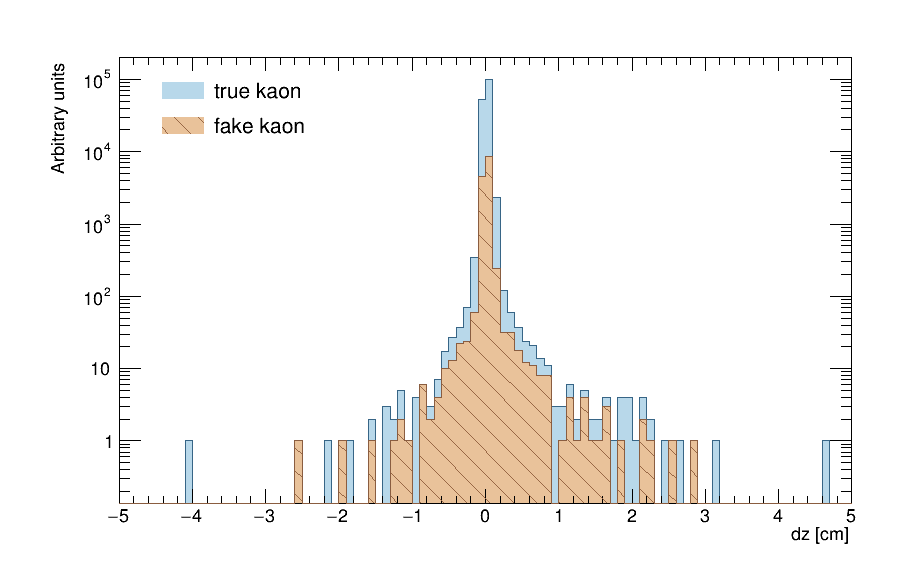
\includegraphics[width=0.47\textwidth]
        {./picture/particle_selections/16_kaon_dz_stack.png}
    }\\
    \subfloat[][\texttt{nCDCHits}]{
        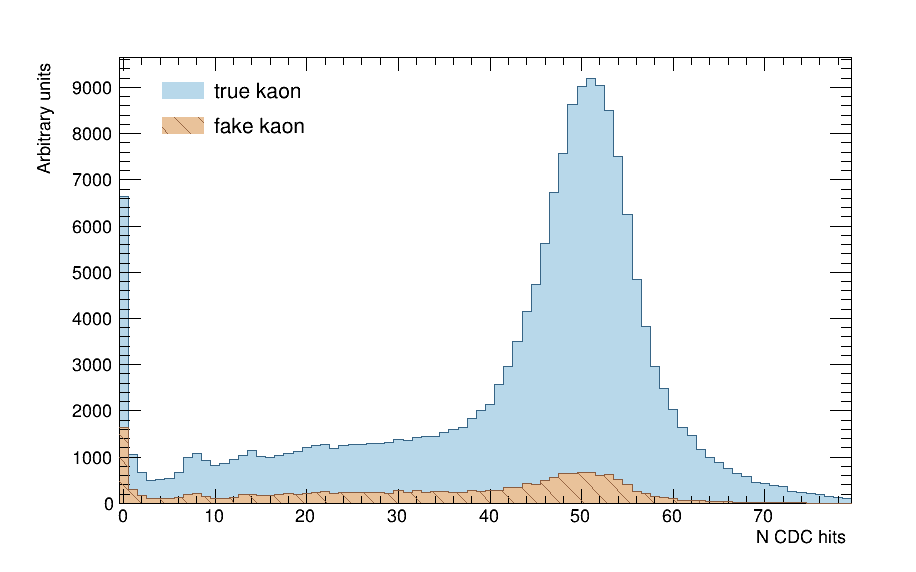
\includegraphics[width=0.47\textwidth]
        {./picture/particle_selections/17_kaon_nCDCHits_stack.png}
    }
    \hfill
    \subfloat[][\texttt{nPXDHits}]{
        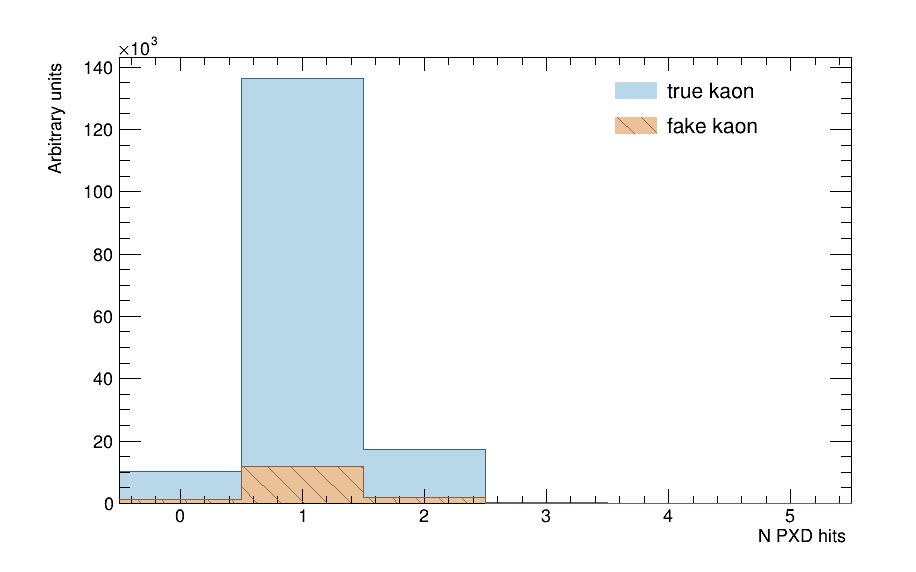
\includegraphics[width=0.47\textwidth]
        {./picture/particle_selections/18_kaon_nPXDHits_stack.png}
    }\\
    \subfloat[][\texttt{kaonID}]{
        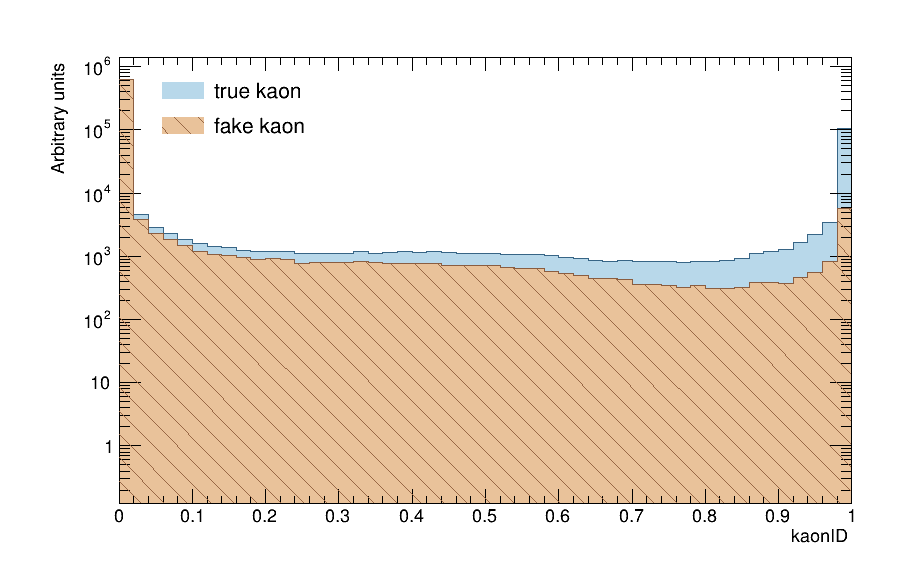
\includegraphics[width=0.47\textwidth]
        {./picture/particle_selections/19_kaon_kaonID_stack.png}
    }
    \caption{
        Distributions of the variables used to select charged kaon
        candidates in the signal MC sample.
        The blue and orange hatched histograms represent true and
        fake candidates, respectively.
        In each panel, the selection requirement on the plotted variable
        is omitted, while all other particle selection requirements
        are applied.
    }
    \label{fig:particle_selection_kaon}
\end{figure}

\begin{figure}[htbp]
    \centering
    \subfloat[][\texttt{clusterNHits}]{
        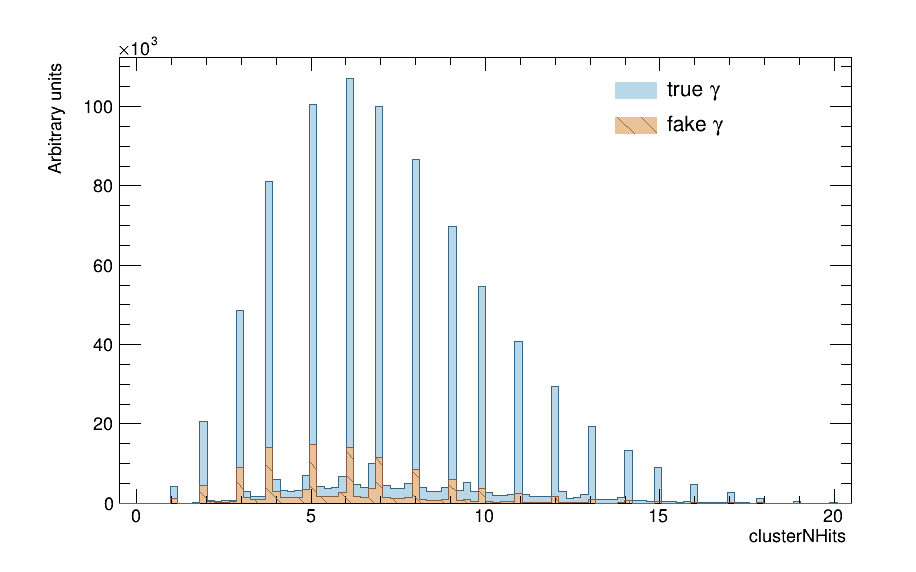
\includegraphics[width=0.47\textwidth]
        {./picture/particle_selections/05_gamma_clusterNHits_stack.png}
    }
    \hfill
    \subfloat[][Polar angle]{
        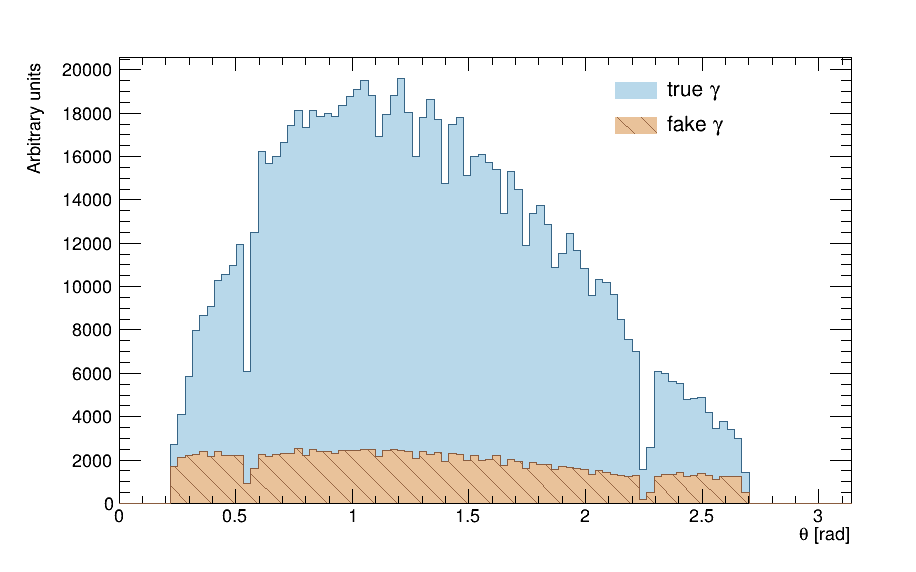
\includegraphics[width=0.47\textwidth]
        {./picture/particle_selections/06_gamma_theta_stack.png}
    }\\
    \subfloat[][Energy]{
        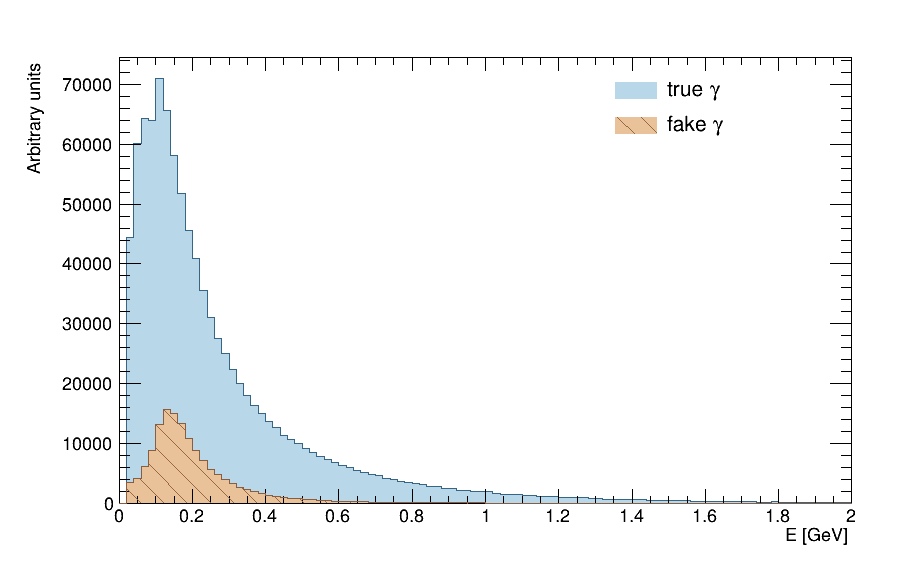
\includegraphics[width=0.47\textwidth]
        {./picture/particle_selections/07_gamma_E_stack.png}
    }
    \caption{
        Distributions of the variables used to select photon
        candidates in the signal MC sample.
        The blue and orange hatched histograms represent true and
        fake candidates, respectively.
        In each panel, the selection requirement on the plotted variable
        is omitted, while all other particle selection requirements
        are applied.
    }
    \label{fig:particle_selection_gamma}
\end{figure}

\begin{figure}[htbp]
    \centering
    \subfloat[][$M_{\gamma\gamma}$]{
        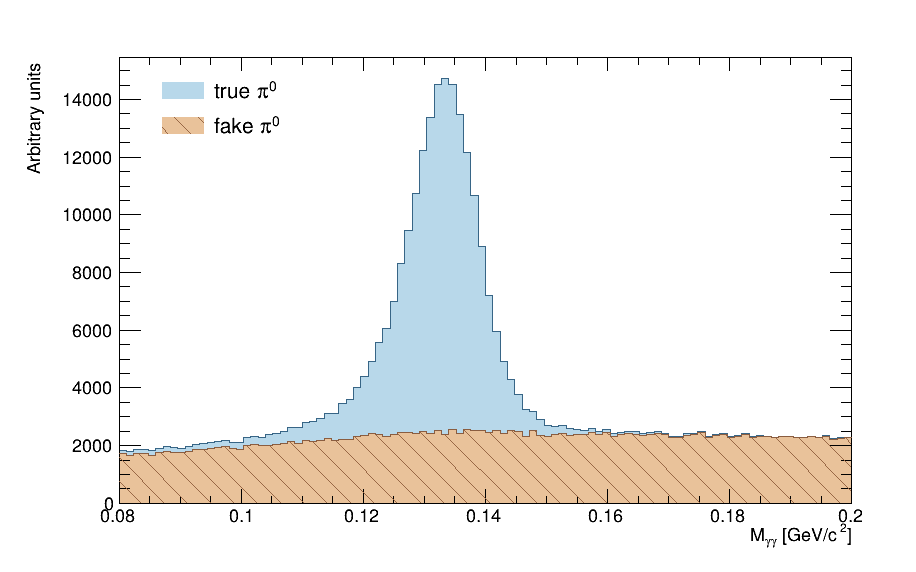
\includegraphics[width=0.47\textwidth]
        {./picture/particle_selections/01_pizero_InvM_stack.png}
    }
    \hfill
    \subfloat[][$\Delta\phi_{\gamma\gamma}$]{
        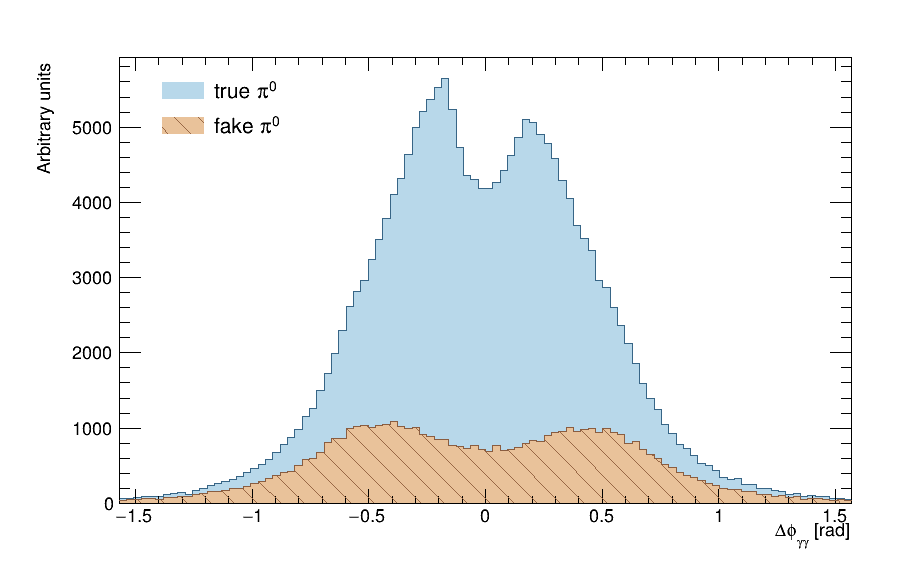
\includegraphics[width=0.47\textwidth]
        {./picture/particle_selections/02_pizero_daughterDiffOf__bo0__cm1__cmphi__bc_stack.png}
    }\\
    \subfloat[][$\Delta\theta_{\gamma\gamma}$]{
        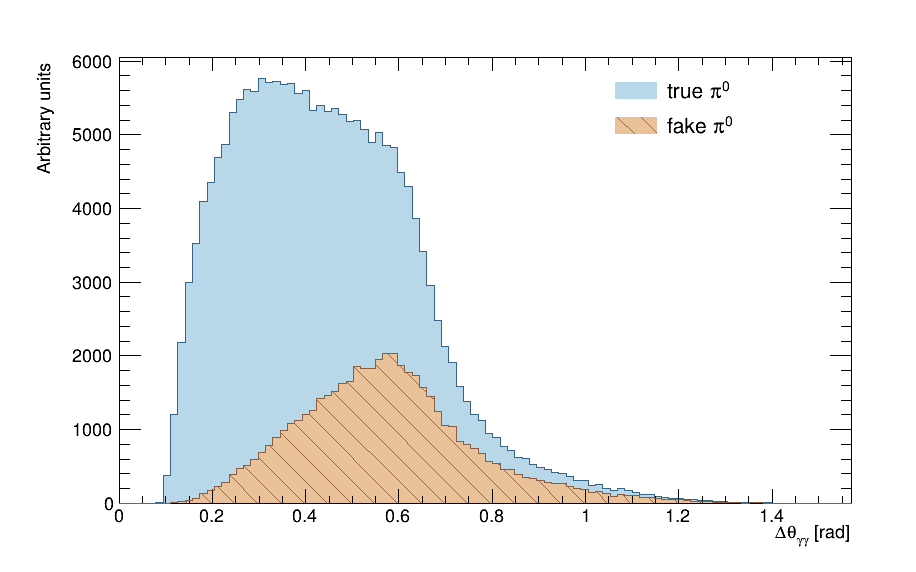
\includegraphics[width=0.47\textwidth]
        {./picture/particle_selections/03_pizero_daughterAngle__bo0__cm1__bc_stack.png}
    }
    \hfill
    \subfloat[][$p_{\pi^0}$]{
        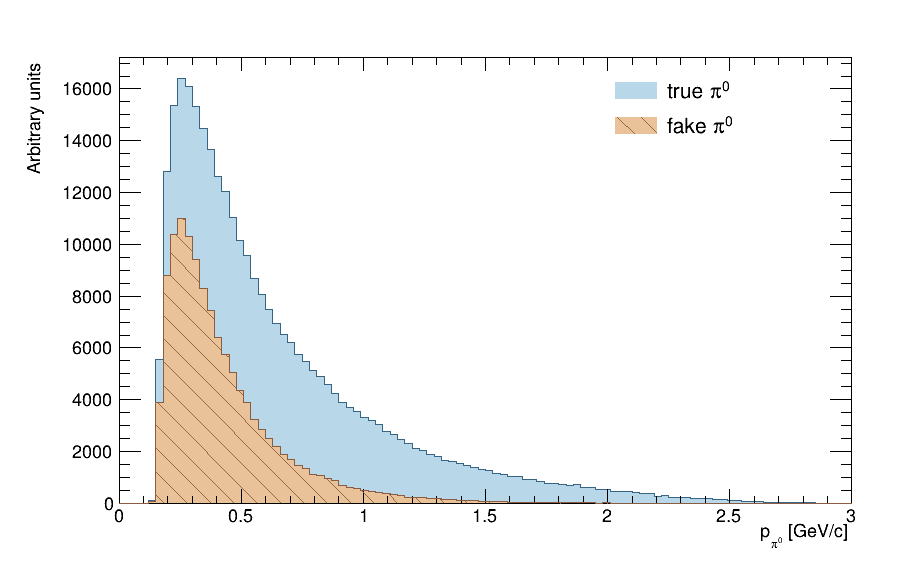
\includegraphics[width=0.47\textwidth]
        {./picture/particle_selections/04_pizero_p_stack.png}
    }
    \caption{
        Distributions of the variables used to select $\pi^0$
        candidates in the signal MC sample.
        The blue and orange hatched histograms represent true and
        fake candidates, respectively.
        In each panel, the selection requirement on the plotted variable
        is omitted, while all other particle selection requirements
        are applied.
    }
    \label{fig:particle_selection_pi0}
\end{figure}

\chapter{FastBDT inputs}
\label{sec:FastBDT_inputs}

\renewcommand{\arraystretch}{1.2}
\setlength{\tabcolsep}{5pt}

\begin{longtable}{
    >{\raggedright\arraybackslash}p{0.39\textwidth}
    >{\raggedright\arraybackslash}p{0.55\textwidth}
}
    \caption{
        List of input variables used for the FastBDT.
        Unless otherwise specified, the ROE denotes the rest of the event
        with respect to $B_{\textrm{tag}}$.
        The reconstruction of the $D$-meson candidates is described in
        Section~\ref{subsec:Dveto_reconstruction}.
        A total of 32 variables are used.
    }
    \label{tab:FastBDT1var}
    \\

    \hline
    \hline
    \multicolumn{1}{c}{FastBDT variable}
    & \multicolumn{1}{c}{Description} \\
    \hline
    \endfirsthead

    \multicolumn{2}{c}{
        \tablename~\thetable{} continued from the previous page
    } \\
    \hline
    \hline
    \multicolumn{1}{c}{FastBDT variable}
    & \multicolumn{1}{c}{Description} \\
    \hline
    \endhead

    \hline
    \multicolumn{2}{r}{Continued on the next page} \\
    \endfoot

    \hline
    \hline
    \endlastfoot

    \path{Bsig_cosTBTO}
    &
    Cosine of the angle between the thrust axis of the $X_{s}$ candidate
    and that of the ROE.
    \\
    \hline

    \path{Bsig_KSFWVariables_hso01},
    \path{Bsig_KSFWVariables_hso04}
    &
    KSFW variables~\cite{Belle:2003fgr} of the $X_{s}$ candidate.
    \\
    \hline

    \path{Bsig_thrustBm}
    &
    Magnitude of the thrust of the $X_{s}$ candidate.
    \\
    \hline

    \path{Bsig_useCMSFrame_p}
    &
    Momentum of the $X_{s}$ candidate in the center-of-mass frame.
    \\
    \hline

    \path{Btag_CleoConeCS_1},
    \path{Btag_CleoConeCS_2},
    \path{Btag_CleoConeCS_3}
    &
    Cleo-cone variables~\cite{CLEO:1995rok} used for continuum suppression.
    \\
    \hline

    \path{Btag_cosTBTO}
    &
    Cosine of the angle between the thrust axis of the
    $B_{\textrm{tag}}$ candidate and that of the ROE.
    \\
    \hline

    \path{Btag_KSFWVariables_hoo1},
    \path{Btag_KSFWVariables_hoo2},
    \path{Btag_KSFWVariables_hoo3},
    \path{Btag_KSFWVariables_hoo4},
    \path{Btag_KSFWVariables_hso02},
    \path{Btag_KSFWVariables_hso24}
    &
    KSFW variables of the $B_{\textrm{tag}}$ candidate.
    \\
    \hline

    \path{Btag_useCMSFrame_theta}
    &
    Polar angle of the $B_{\textrm{tag}}$ candidate in the
    center-of-mass frame.
    \\
    \hline

    \path{extraInfo__boEeclv200}
    &
    Extra energy deposited in the ECL.
    \\
    \hline

    \path{extraInfo__boNgammav200__bc}
    &
    Number of photon candidates in the ROE.
    \\
    \hline

    \path{foxWolframR3},
    \path{foxWolframR4}
    &
    Ratios of the third- and fourth-order Fox--Wolfram moments
    to the zeroth-order moment, respectively~\cite{Fox:1978vw}.
    \\
    \hline

    \path{harmonicMomentThrust1},
    \path{harmonicMomentThrust2}
    &
    Harmonic moments calculated with respect to the thrust axis~\cite{Fox:1978vw}.
    \\
    \hline

    \path{missingMomentumOfEvent}
    &
    Magnitude of the missing momentum in the laboratory frame.
    \\
    \hline

    \path{missingMomentumOfEvent_theta}
    &
    Polar angle of the missing momentum in the laboratory frame.
    \\
    \hline

    \path{nRemainingTracksInEvent}
    &
    Number of tracks in the ROE before applying additional track selections.
    \\
    \hline

    \path{roePTheta__bocleanMask__bc}
    &
    Polar angle of the ROE momentum.
    Here, the ROE is defined with respect to the
    $B_{\textrm{tag}}$ and $X_{s}$ candidates.
    \\
    \hline

    \path{Bsig_daughter_0_extraInfo_Dc_pValue_std_noDCS}
    &
    Standard deviation of the vertex-fit $p$-values for $D^{\pm}$ in the first category.
    \\
    \hline

    \path{Bsig_daughter_0_extraInfo_Dcsimpleveto_M_noDCS}
    &
    Mass of the $D^{\pm}$ candidate with the highest vertex-fit $p$-value in the first category.
    \\
    \hline

    \path{Bsig_daughter_0_extraInfo_D0_pValue_std}
    &
    Standard deviation of the vertex-fit $p$-values for $D^{0}$ in the second category.
    \\
    \hline

    \path{Bsig_daughter_0_extraInfo_D0simpleveto_M}
    &
    Mass of the $D^0$ candidate with the highest vertex-fit $p$-value in the second category.
    \\
    \hline

    \path{Bsig_daughter_0_extraInfo_D0_pValue_std_yespizero}
    &
    Standard deviation of the vertex-fit $p$-values for $D^{0}$ in the fourth category.
    \\
    \hline

    \path{Bsig_daughter_0_extraInfo_D0simpleveto_M_yespizero}
    &
    Mass of the $D^{0}$ candidate with the highest vertex-fit $p$-value in the fourth category.
    \\

\end{longtable}

\chapter{Efficiency as a function of $M_{X_{s}}$}
\label{sec:efficiency_as_MXs}
\begin{figure}[h]
  \centering
  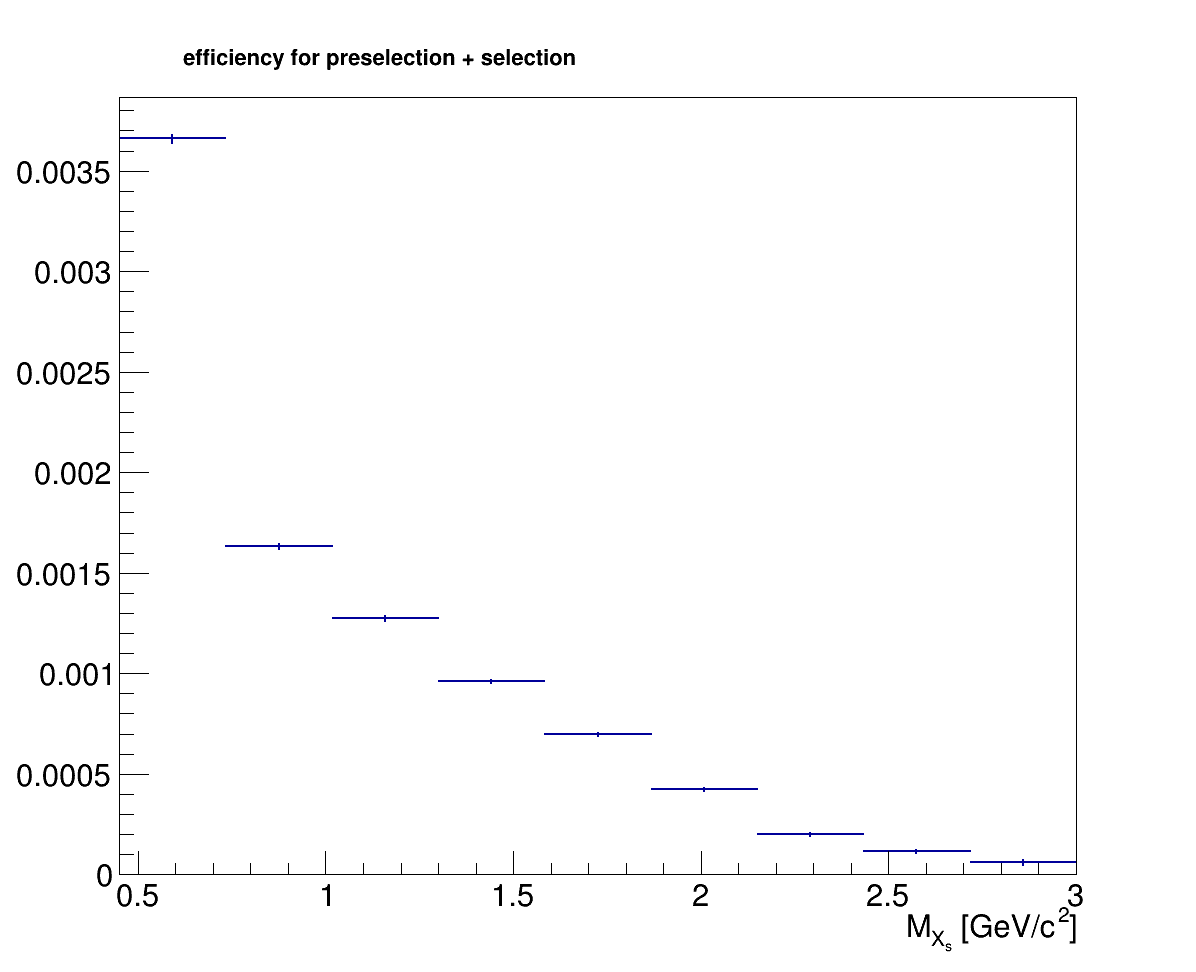
\includegraphics[width=0.45\textwidth]{./picture/eff/Efficiency.png}
  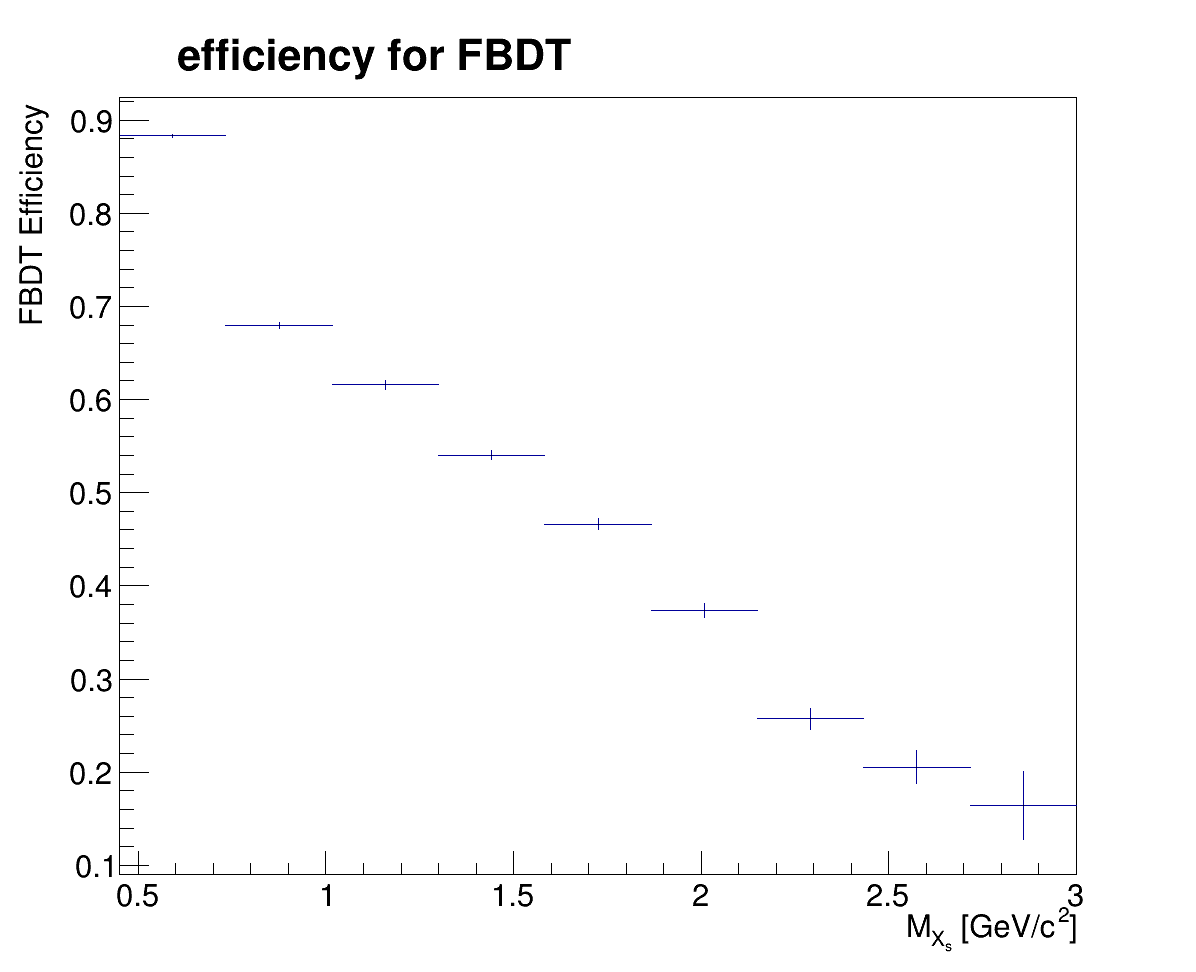
\includegraphics[width=0.45\textwidth]{./picture/eff/FBDT_Efficiency.png}
  \caption{Signal efficiency as a function of the true $X_{s}$ mass, $M_{X_{s}}$. The left plot shows the combined efficiency of the preselection and selection requirements, and the right plot shows the efficiency of the FastBDT output requirement. The efficiency decreases with increasing $M_{X_{s}}$.}
  \label{fig:eff_Mxs}
\end{figure}
\begin{figure}[h]
  \centering
  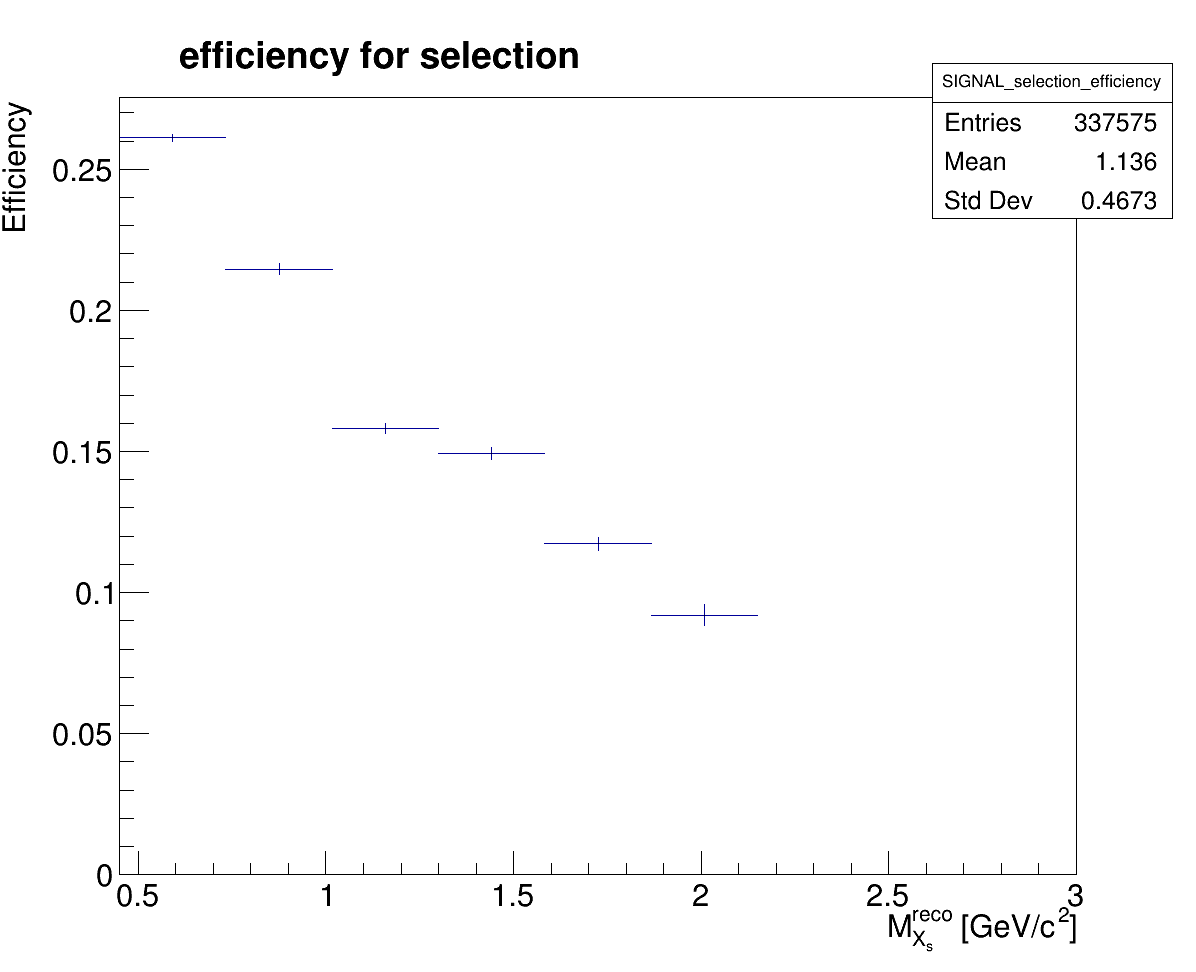
\includegraphics[width=0.45\textwidth]{./picture/eff/Signal_eff_reco.png}
  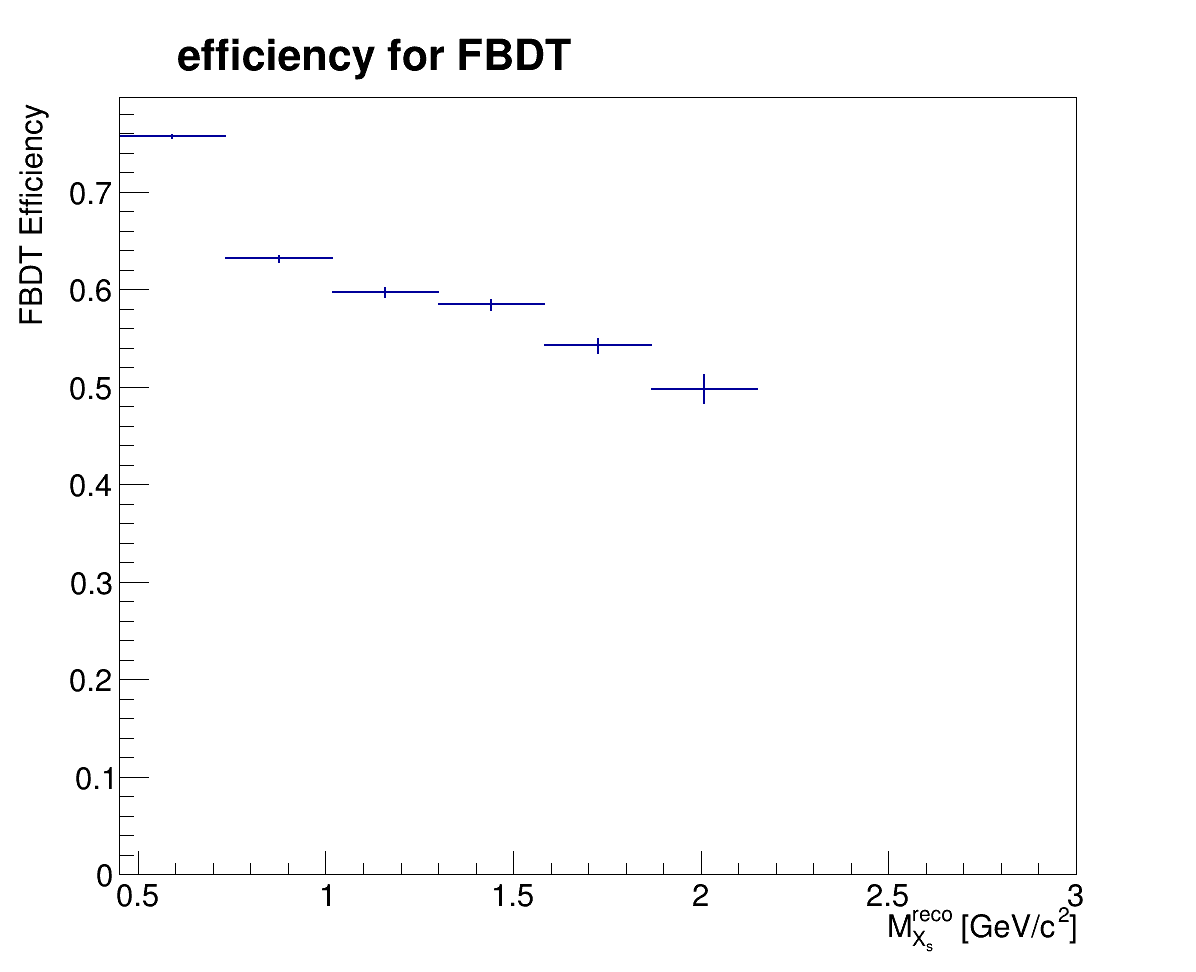
\includegraphics[width=0.45\textwidth]{./picture/eff/Signal_FBDT_reco.png}
  \caption{Signal efficiency as a function of the reconstructed $X_{s}$ mass, $M_{X_{s}}^{\textrm{reco}}$. The left plot shows the efficiency of the selection requirements, and the right plot shows the efficiency of the FastBDT output requirement. The efficiency decreases with increasing $M_{X_{s}}^{\textrm{reco}}$.}
  \label{fig:eff_Mxs_sig_reco}
\end{figure}
\begin{figure}[h]
  \centering
  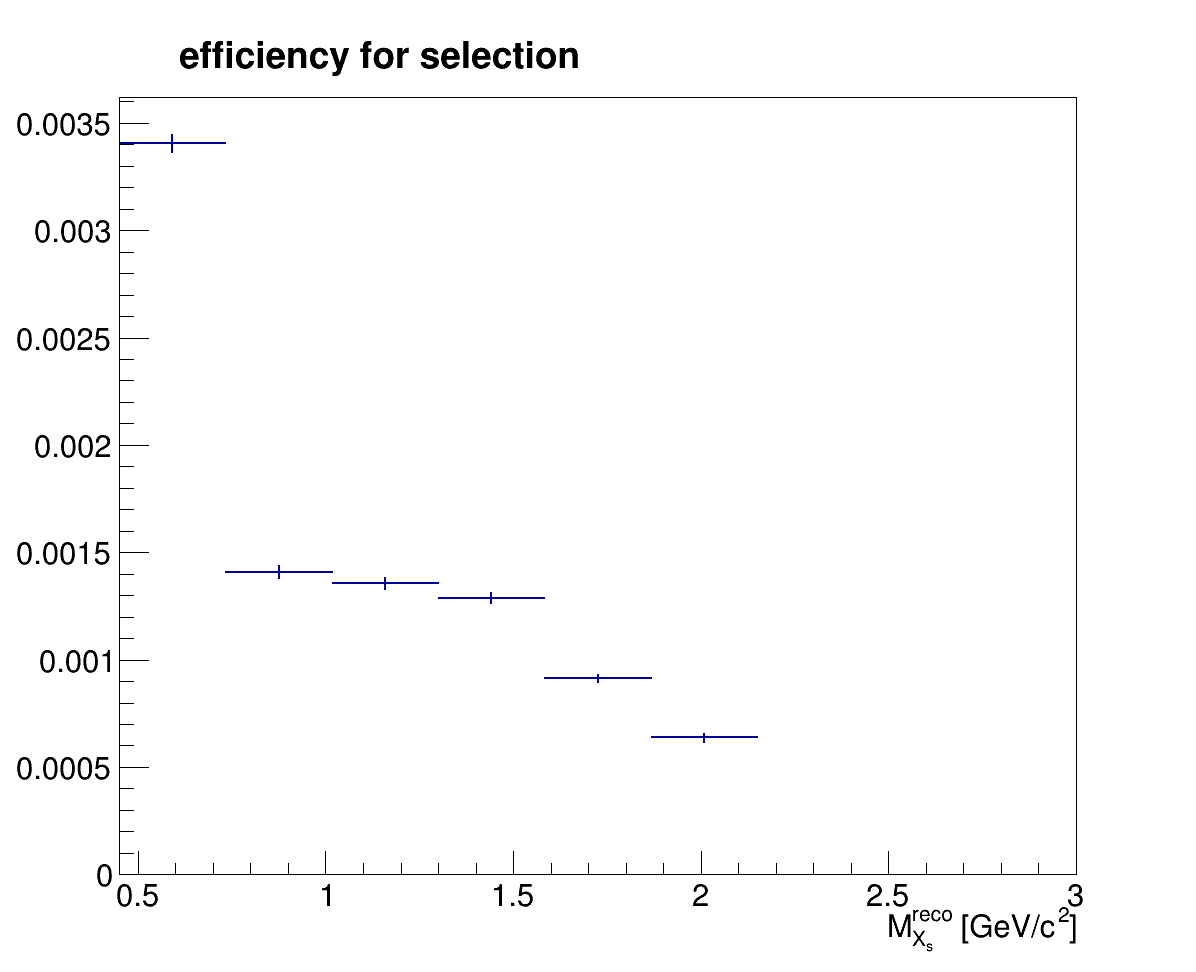
\includegraphics[width=0.45\textwidth]{./picture/eff/Background_eff_reco.png}
  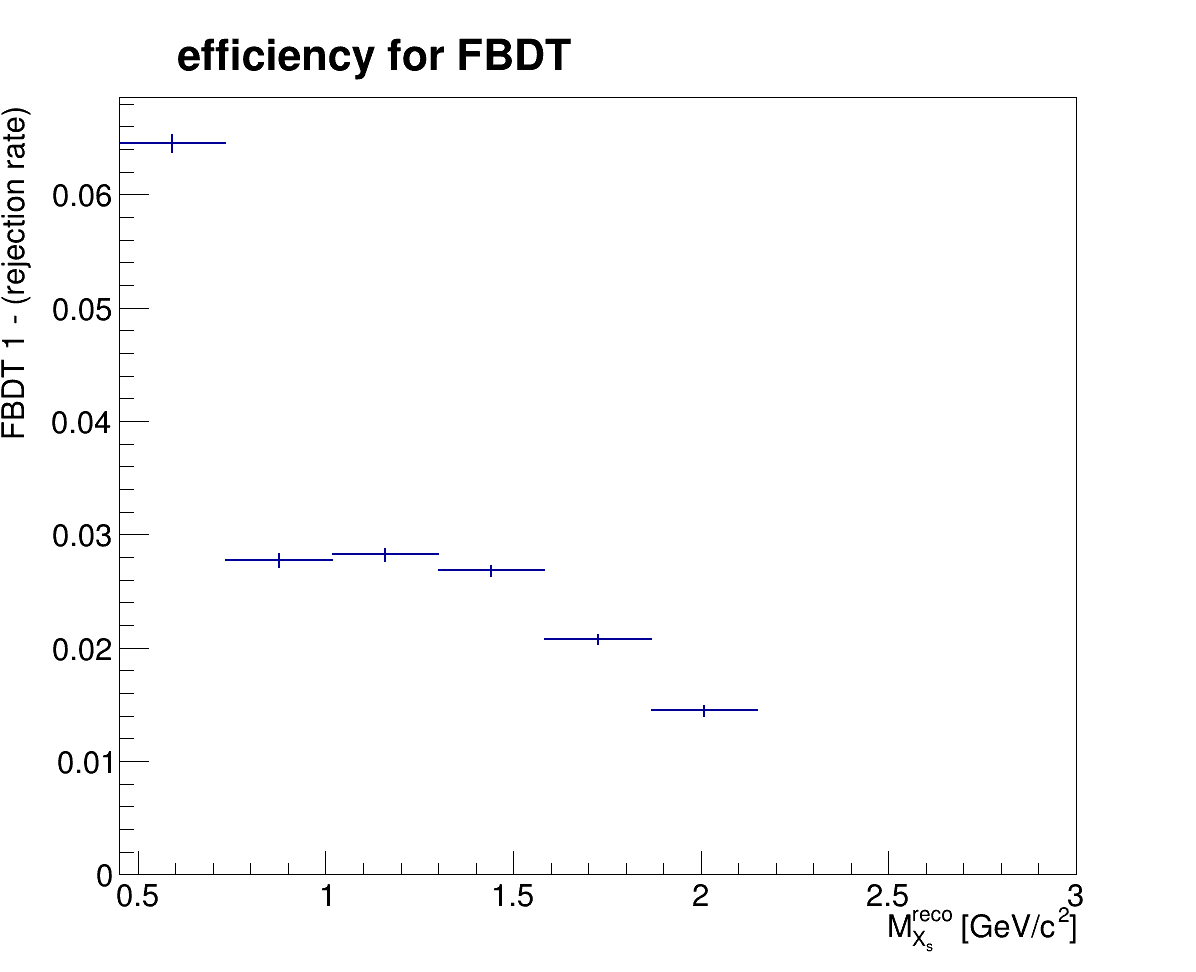
\includegraphics[width=0.45\textwidth]{./picture/eff/Background_FBDT.png}
  \caption{Background efficiency as a function of the reconstructed $X_{s}$ mass, $M_{X_{s}}^{\textrm{reco}}$. The left plot shows the efficiency of the selection requirements, and the right plot shows the efficiency of the FastBDT output requirement. The background efficiency decreases with increasing $M_{X_{s}}^{\textrm{reco}}$.}
  \label{fig:eff_Mxs_bkg_reco}
\end{figure}

\chapter{FastBDT input variable distributions}
\begin{figure}[h]
    \centering

    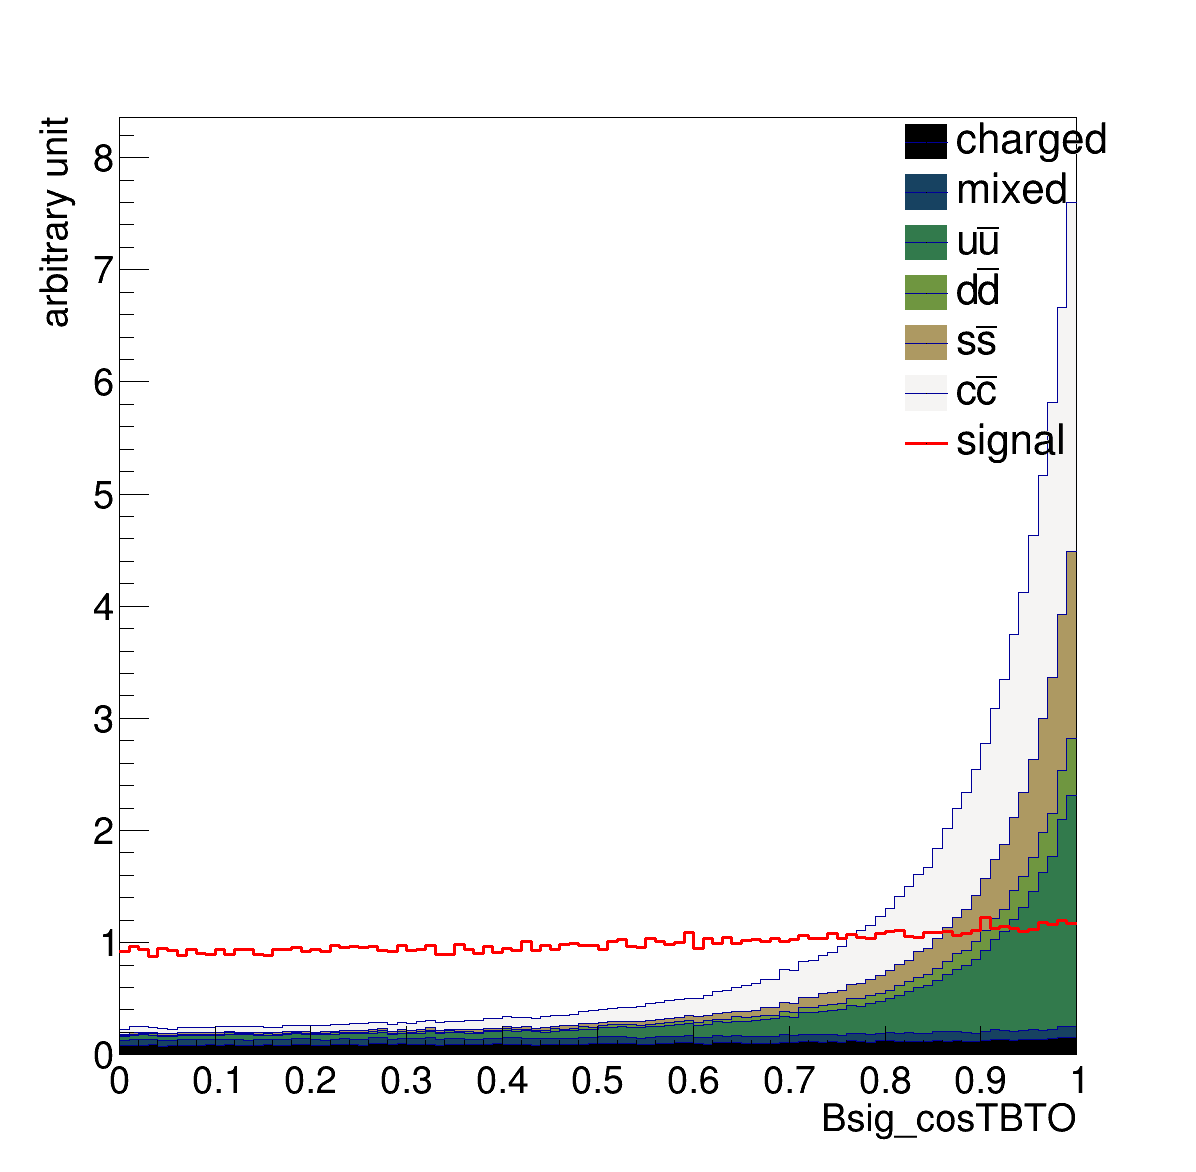
\includegraphics[width=0.24\textwidth]{./picture/FBDT_input/Bsig_cosTBTO.png}
    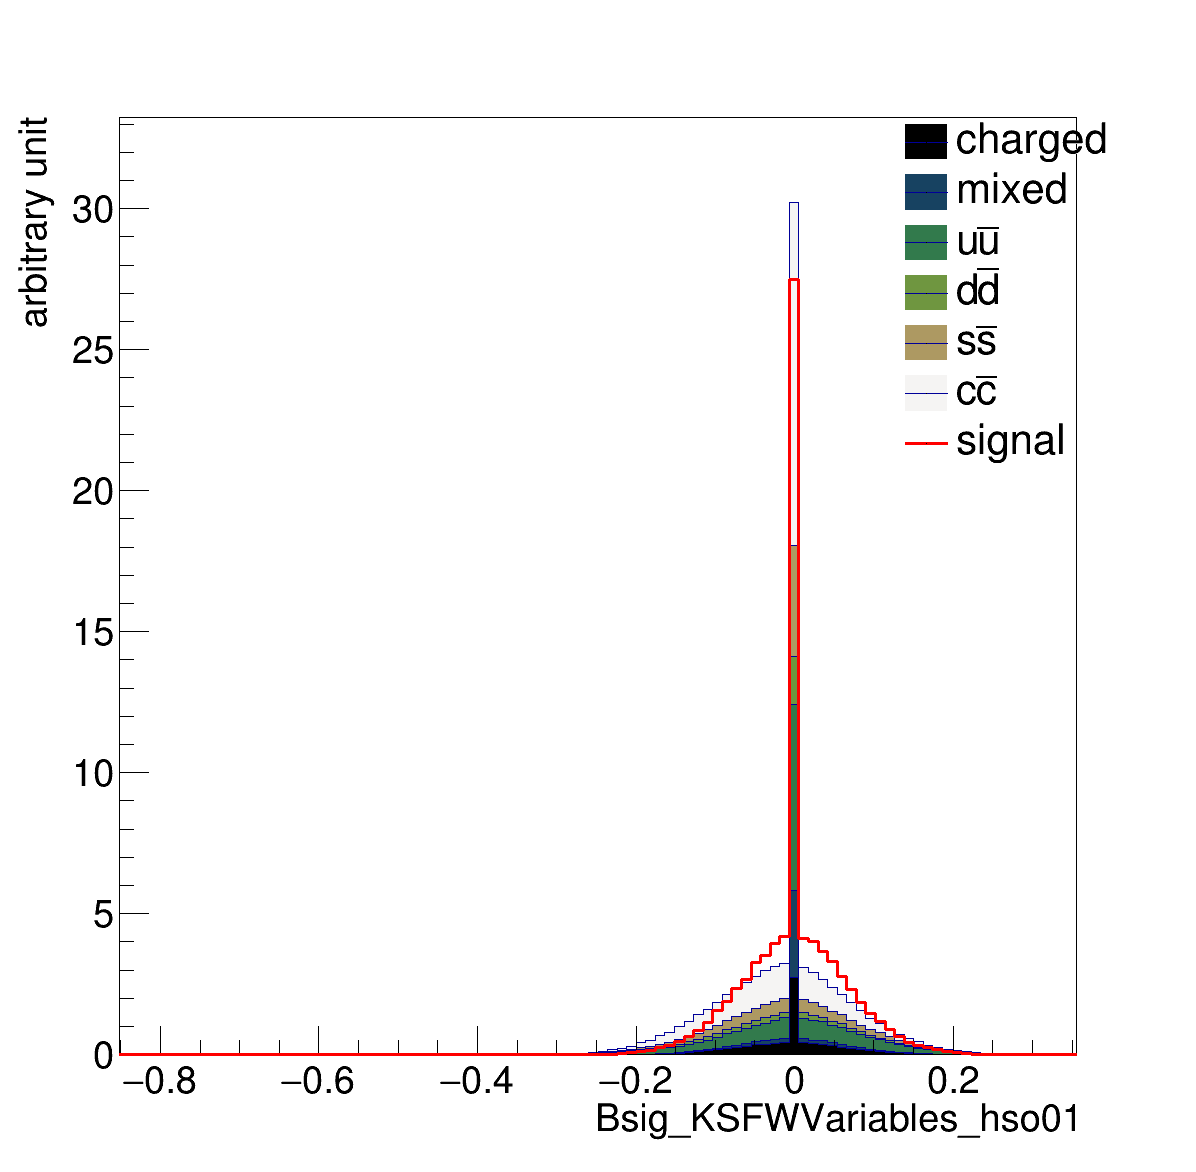
\includegraphics[width=0.24\textwidth]{./picture/FBDT_input/Bsig_KSFWVariables_hso01.png}
    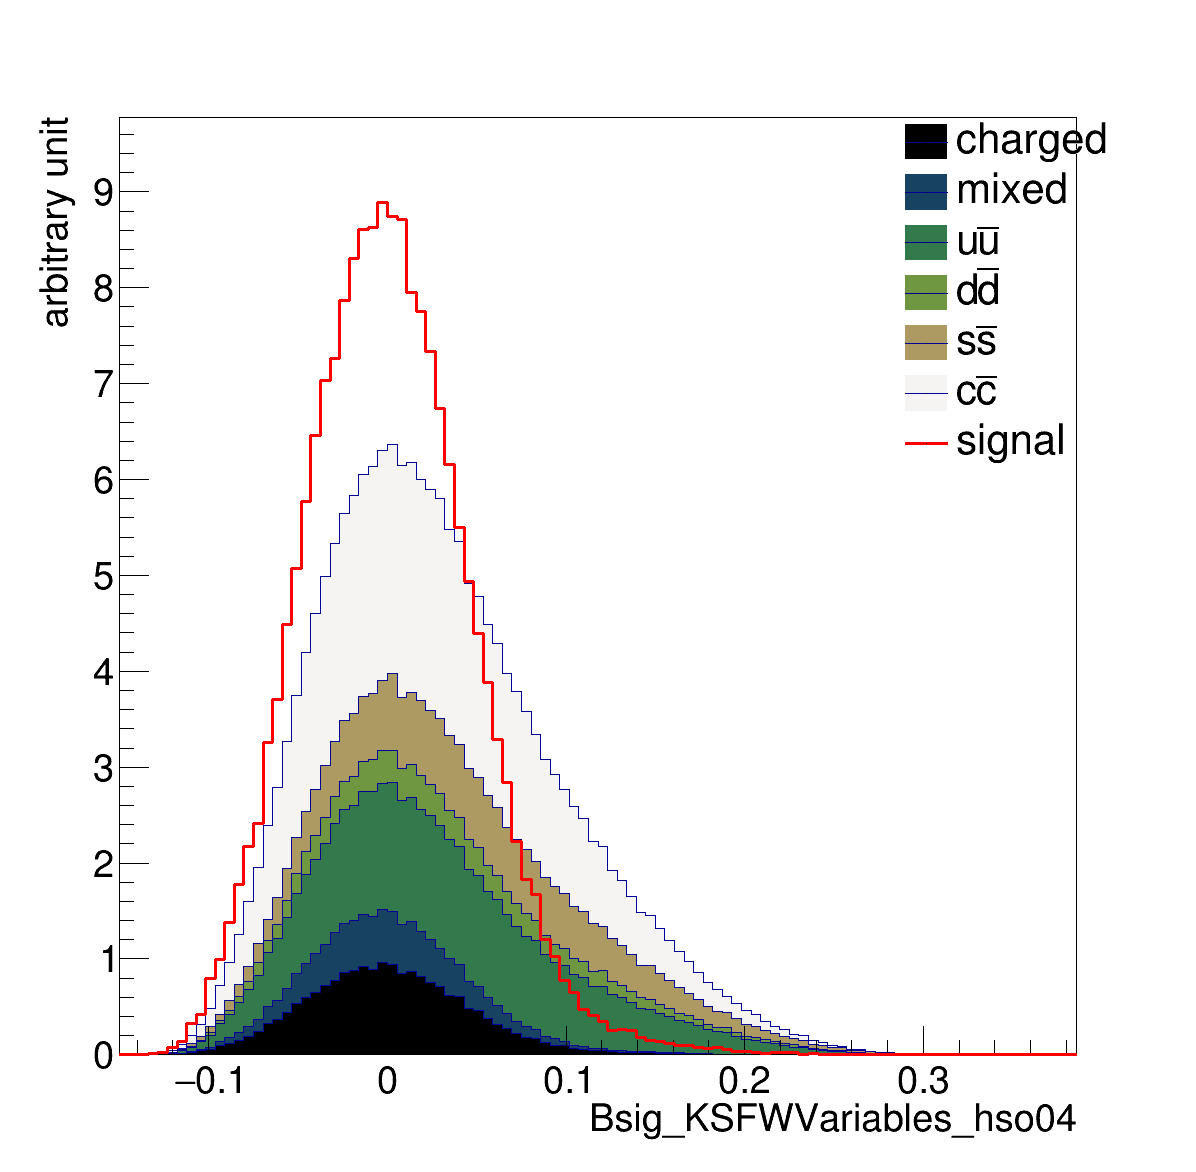
\includegraphics[width=0.24\textwidth]{./picture/FBDT_input/Bsig_KSFWVariables_hso04.png}
    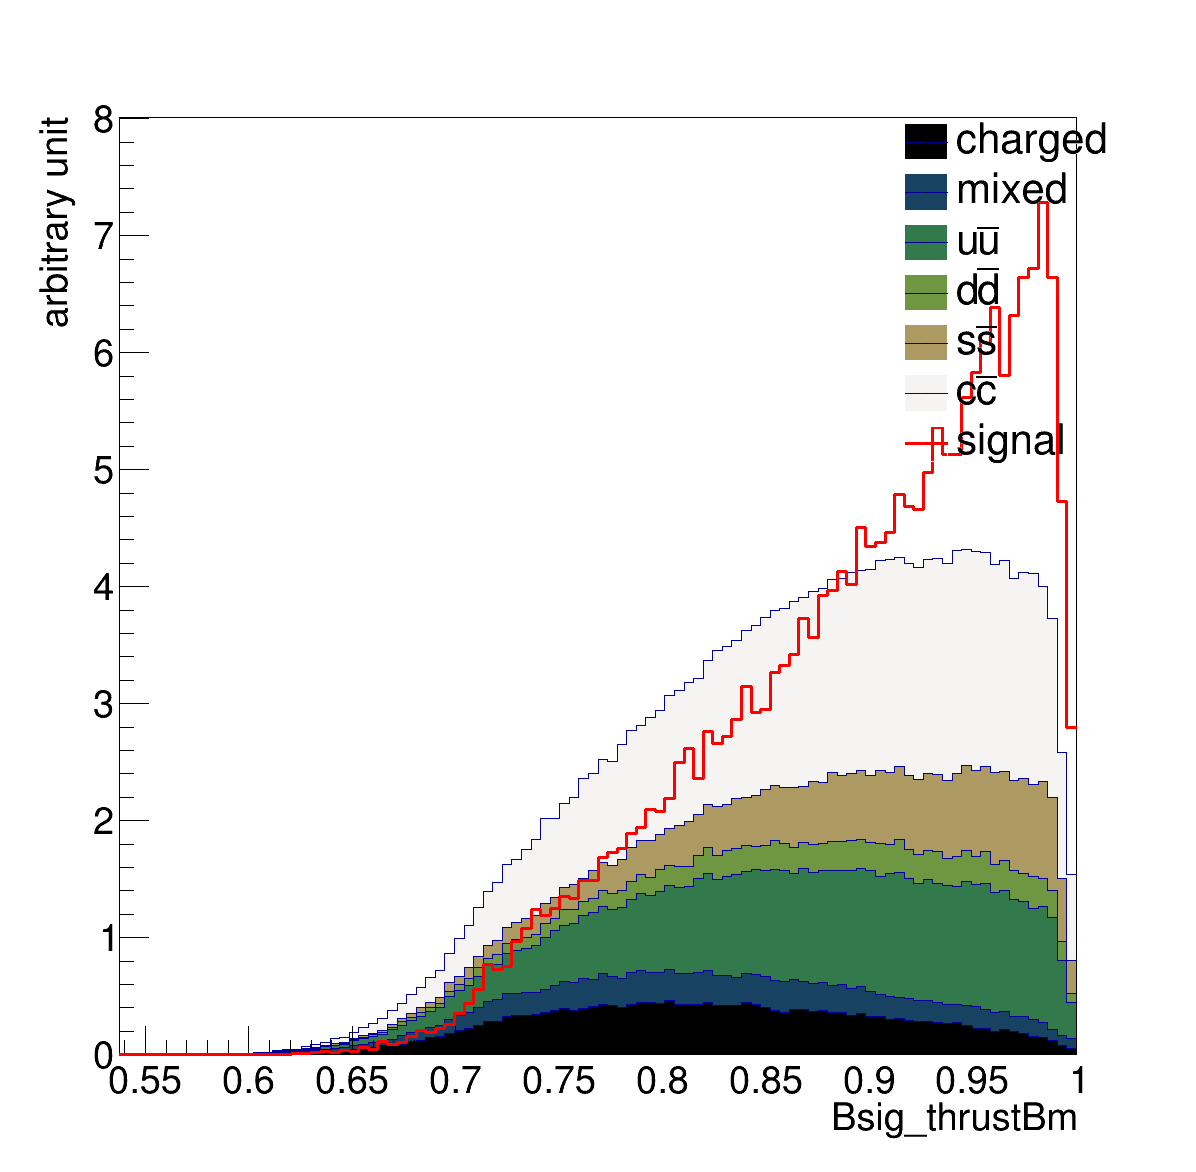
\includegraphics[width=0.24\textwidth]{./picture/FBDT_input/Bsig_thrustBm.png}

    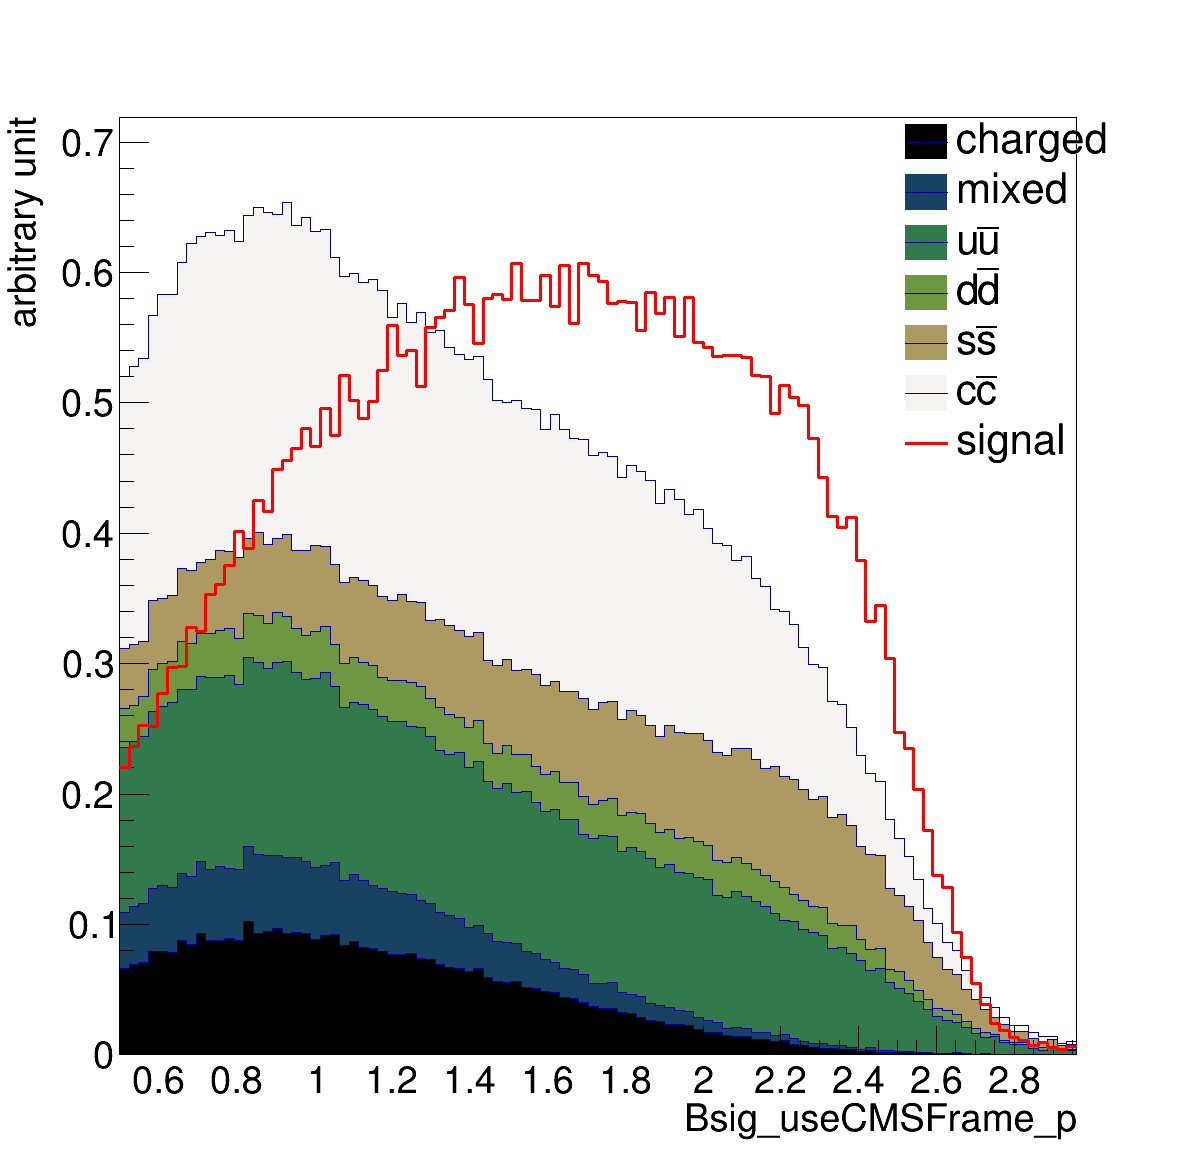
\includegraphics[width=0.24\textwidth]{./picture/FBDT_input/Bsig_useCMSFrame_p.png}
    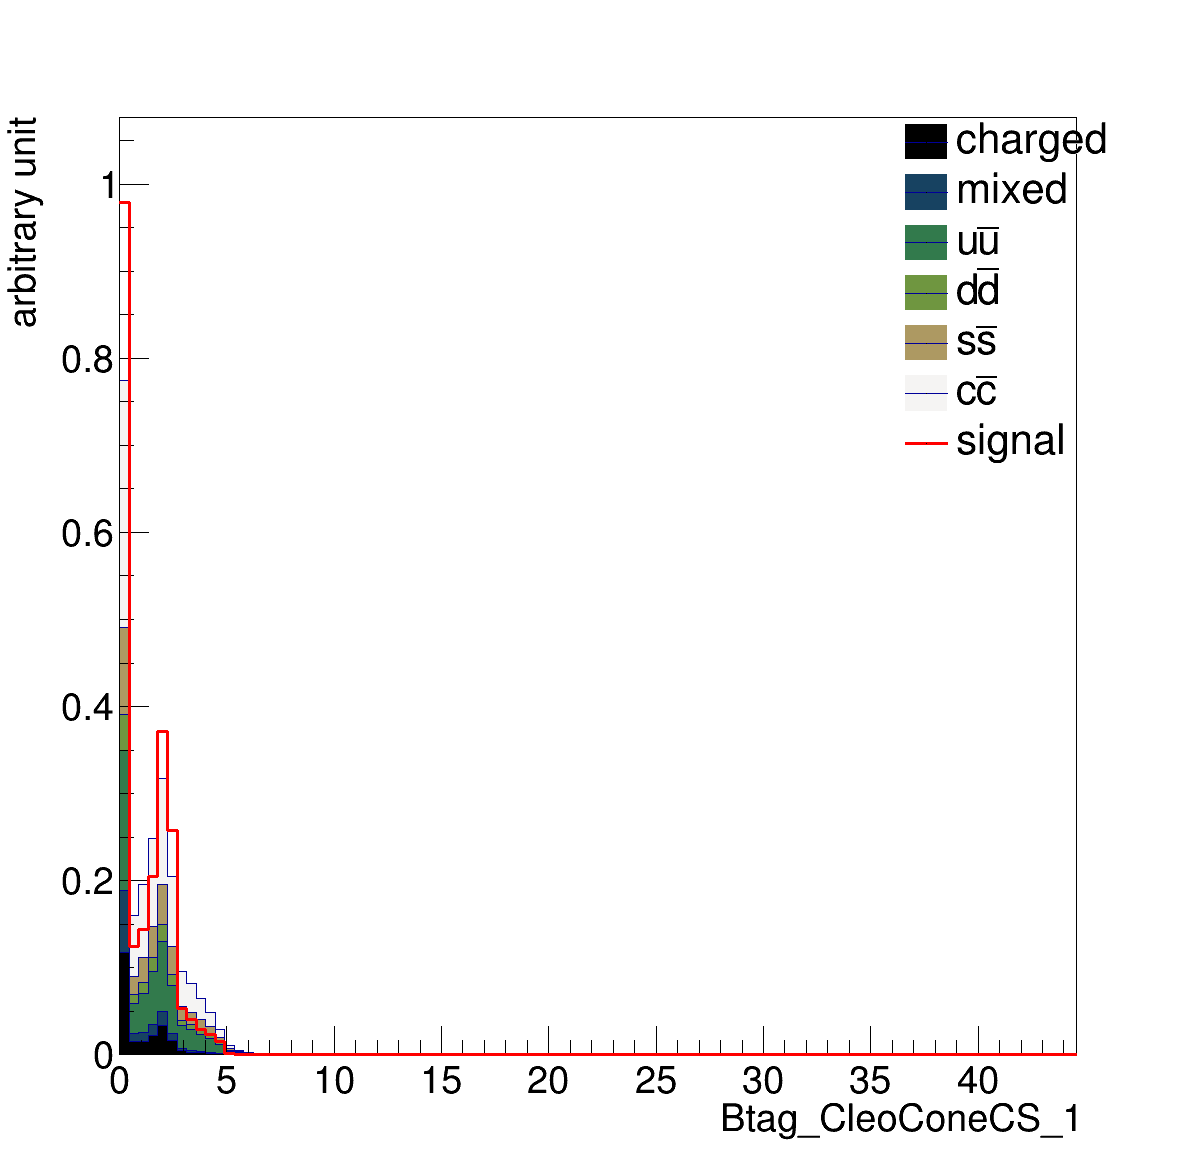
\includegraphics[width=0.24\textwidth]{./picture/FBDT_input/Btag_CleoConeCS_1.png}
    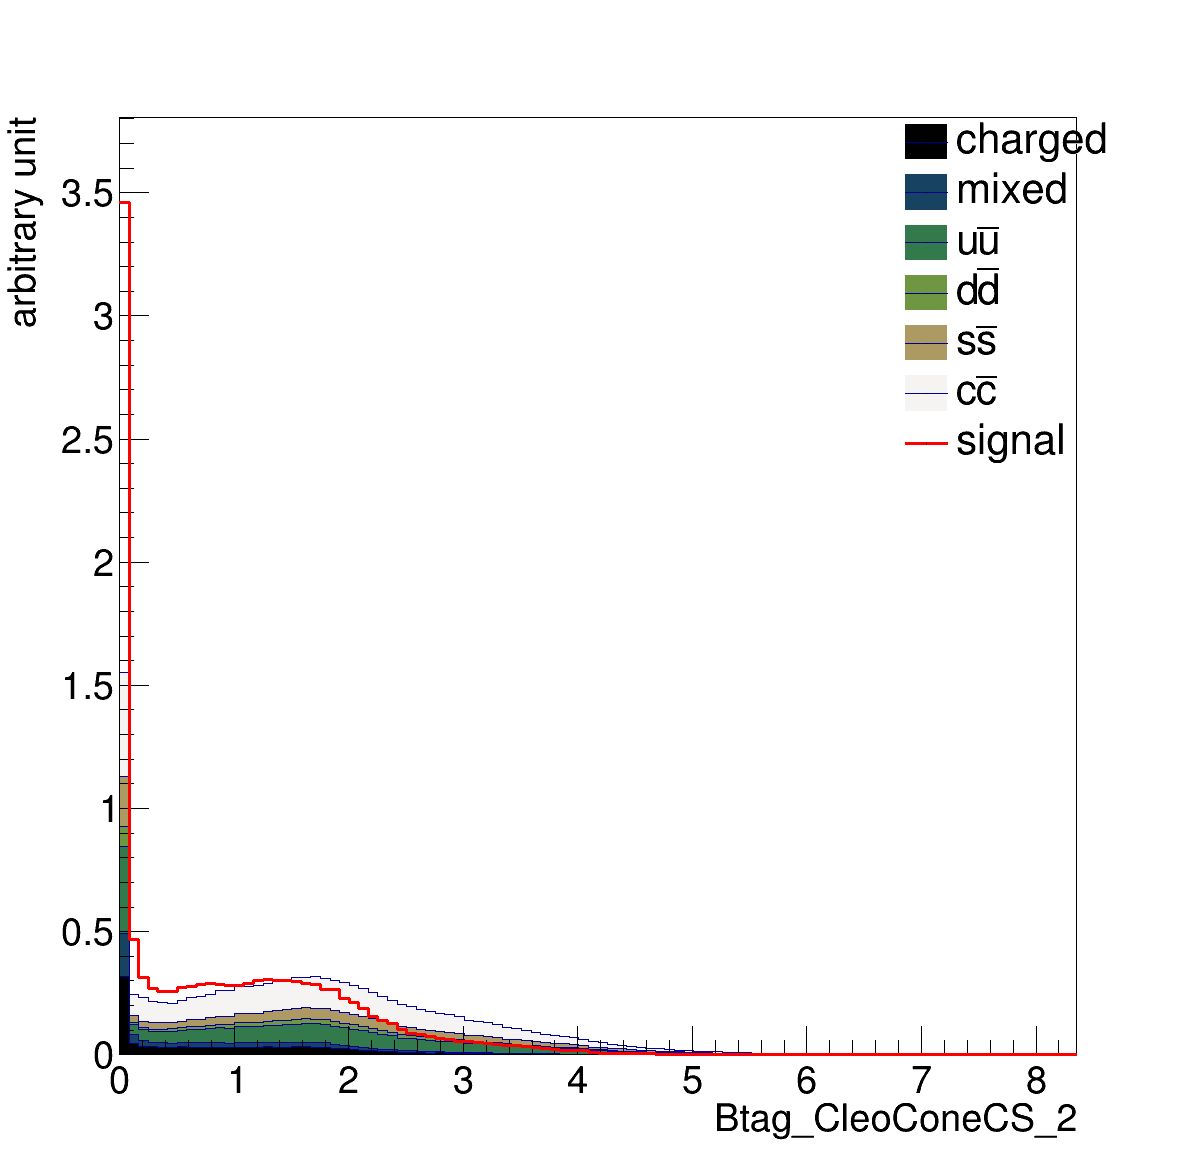
\includegraphics[width=0.24\textwidth]{./picture/FBDT_input/Btag_CleoConeCS_2.png}
    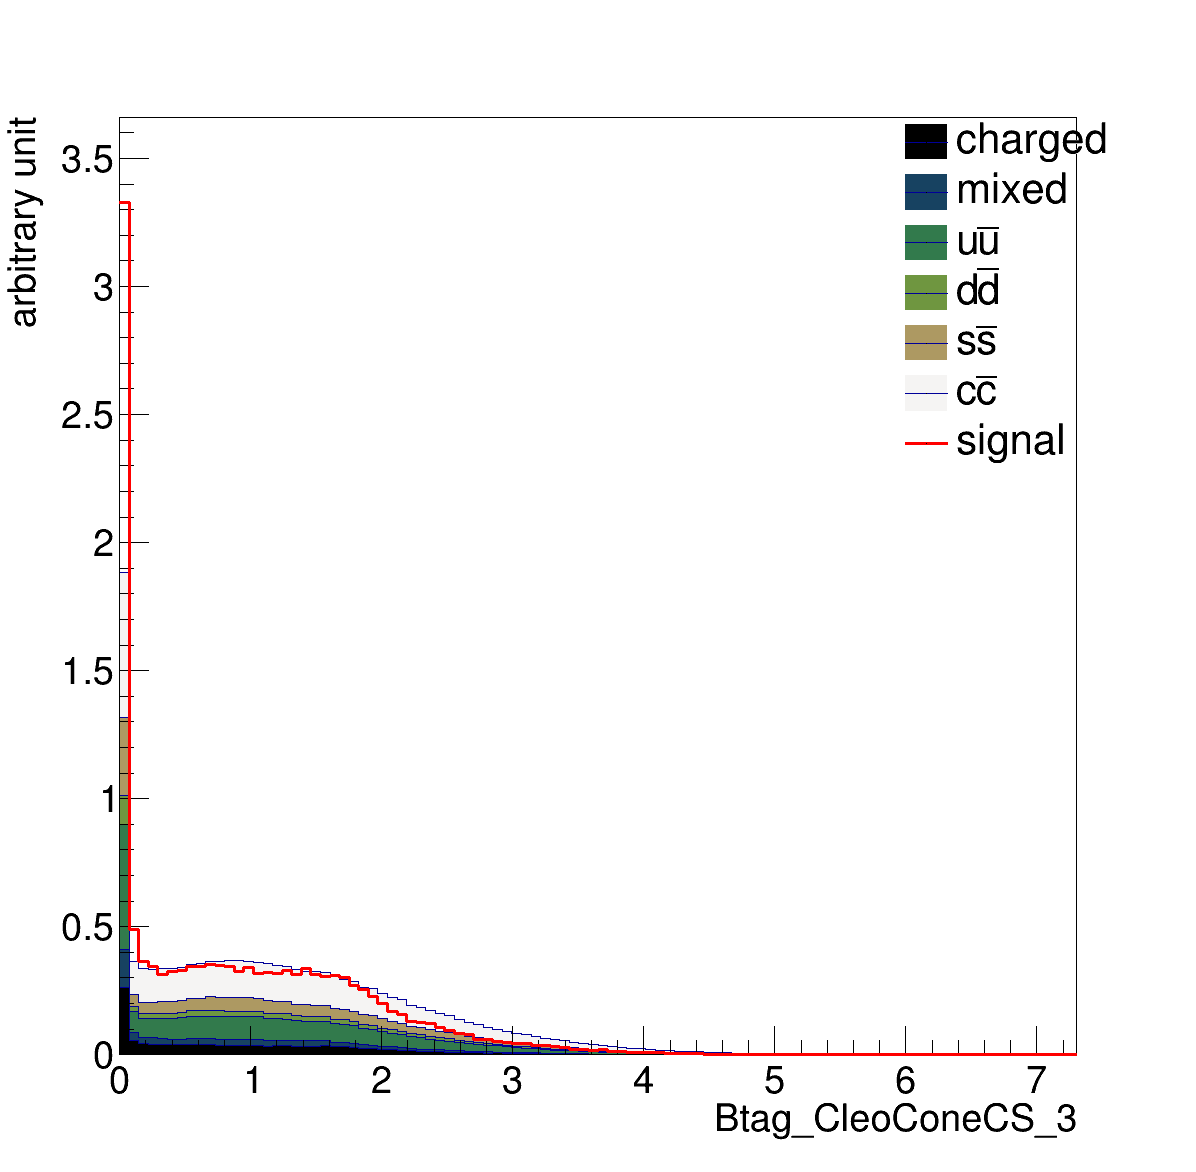
\includegraphics[width=0.24\textwidth]{./picture/FBDT_input/Btag_CleoConeCS_3.png}

    \includegraphics[width=0.24\textwidth]{./picture/FBDT_input/Btag_cosTBTO.png}
    \includegraphics[width=0.24\textwidth]{./picture/FBDT_input/Btag_KSFWVariables_hoo1.png}
    \includegraphics[width=0.24\textwidth]{./picture/FBDT_input/Btag_KSFWVariables_hoo2.png}
    \includegraphics[width=0.24\textwidth]{./picture/FBDT_input/Btag_KSFWVariables_hoo3.png}

    \includegraphics[width=0.24\textwidth]{./picture/FBDT_input/Btag_KSFWVariables_hoo4.png}
    \includegraphics[width=0.24\textwidth]{./picture/FBDT_input/Btag_KSFWVariables_hso02.png}
    \includegraphics[width=0.24\textwidth]{./picture/FBDT_input/Btag_KSFWVariables_hso24.png}
    \includegraphics[width=0.24\textwidth]{./picture/FBDT_input/Btag_useCMSFrame_theta.png}

    \caption{FastBDT input variables.}
    \label{fig:FastBDTinputs1}
\end{figure}
\begin{figure}[h]
    \centering

    \includegraphics[width=0.24\textwidth]{./picture/FBDT_input/extraInfo__boEeclv200__bc.png}
    \includegraphics[width=0.24\textwidth]{./picture/FBDT_input/extraInfo__boNgammav200__bc.png}
    \includegraphics[width=0.24\textwidth]{./picture/FBDT_input/foxWolframR3.png}
    \includegraphics[width=0.24\textwidth]{./picture/FBDT_input/foxWolframR4.png}

    \includegraphics[width=0.24\textwidth]{./picture/FBDT_input/harmonicMomentThrust1.png}
    \includegraphics[width=0.24\textwidth]{./picture/FBDT_input/harmonicMomentThrust2.png}
    \includegraphics[width=0.24\textwidth]{./picture/FBDT_input/missingMomentumOfEvent.png}
    \includegraphics[width=0.24\textwidth]{./picture/FBDT_input/missingMomentumOfEvent_theta.png}

    \includegraphics[width=0.24\textwidth]{./picture/FBDT_input/nRemainingTracksInEvent.png}
    \includegraphics[width=0.24\textwidth]{./picture/FBDT_input/roePTheta__bocleanMask__bc.png}
    \includegraphics[width=0.24\textwidth]{./picture/FBDT_input/Bsig_daughter_0_extraInfo_Dc_pValue_std.png}
    \includegraphics[width=0.24\textwidth]{./picture/FBDT_input/Bsig_daughter_0_extraInfo_Dcsimpleveto_M.png}

    \includegraphics[width=0.24\textwidth]{./picture/FBDT_input/Bsig_daughter_0_extraInfo_D0_pValue_std.png}
    \includegraphics[width=0.24\textwidth]{./picture/FBDT_input/Bsig_daughter_0_extraInfo_D0simpleveto_M.png}

    \caption{FastBDT input variables.}
    \label{fig:FastBDTinputs2}
\end{figure}

\chapter{Off-resonance variable distributions}
\label{sec:off_variables}
\begin{figure}[h]
    \centering

    \includegraphics[width=0.24\textwidth]{./picture/off/Bsig_cosTBTO_offres.png}
    \includegraphics[width=0.24\textwidth]{./picture/off/Bsig_KSFWVariables_hso01_offres.png}
    \includegraphics[width=0.24\textwidth]{./picture/off/Bsig_KSFWVariables_hso04_offres.png}
    \includegraphics[width=0.24\textwidth]{./picture/off/Bsig_thrustBm_offres.png}
    
    \includegraphics[width=0.24\textwidth]{./picture/off/Bsig_useCMSFrame_p_offres.png}
    \includegraphics[width=0.24\textwidth]{./picture/off/Btag_CleoConeCS_1_offres.png}
    \includegraphics[width=0.24\textwidth]{./picture/off/Btag_CleoConeCS_2_offres.png}
    \includegraphics[width=0.24\textwidth]{./picture/off/Btag_CleoConeCS_3_offres.png}
    
    \includegraphics[width=0.24\textwidth]{./picture/off/Btag_cosTBTO_offres.png}
    \includegraphics[width=0.24\textwidth]{./picture/off/Btag_KSFWVariables_hoo1_offres.png}
    \includegraphics[width=0.24\textwidth]{./picture/off/Btag_KSFWVariables_hoo2_offres.png}
    \includegraphics[width=0.24\textwidth]{./picture/off/Btag_KSFWVariables_hoo3_offres.png}
    
    \includegraphics[width=0.24\textwidth]{./picture/off/Btag_KSFWVariables_hoo4_offres.png}
    \includegraphics[width=0.24\textwidth]{./picture/off/Btag_KSFWVariables_hso02_offres.png}
    \includegraphics[width=0.24\textwidth]{./picture/off/Btag_KSFWVariables_hso24_offres.png}
    \includegraphics[width=0.24\textwidth]{./picture/off/Btag_useCMSFrame_theta_offres.png}

    \caption{FastBDT input variables.}
    \label{fig:off_used_vars1}
\end{figure}
\begin{figure}[h]
    \centering

    \includegraphics[width=0.24\textwidth]{./picture/off/extraInfo__boEeclv200__bc_offres.png}
    \includegraphics[width=0.24\textwidth]{./picture/off/extraInfo__boNgammav200__bc_offres.png}
    \includegraphics[width=0.24\textwidth]{./picture/off/foxWolframR3_offres.png}
    \includegraphics[width=0.24\textwidth]{./picture/off/foxWolframR4_offres.png}

    \includegraphics[width=0.24\textwidth]{./picture/off/harmonicMomentThrust1_offres.png}
    \includegraphics[width=0.24\textwidth]{./picture/off/harmonicMomentThrust2_offres.png}
    \includegraphics[width=0.24\textwidth]{./picture/off/missingMomentumOfEvent_offres.png}
    \includegraphics[width=0.24\textwidth]{./picture/off/missingMomentumOfEvent_theta_offres.png}

    \includegraphics[width=0.24\textwidth]{./picture/off/nRemainingTracksInEvent_offres.png}
    \includegraphics[width=0.24\textwidth]{./picture/off/roePTheta__bocleanMask__bc_offres.png}
    \includegraphics[width=0.24\textwidth]{./picture/off/Bsig_daughter_0_extraInfo_Dc_pValue_std_offres.png}
    \includegraphics[width=0.24\textwidth]{./picture/off/Bsig_daughter_0_extraInfo_Dcsimpleveto_M_offres.png}

    \includegraphics[width=0.24\textwidth]{./picture/off/Bsig_daughter_0_extraInfo_D0_pValue_std_offres.png}
    \includegraphics[width=0.24\textwidth]{./picture/off/Bsig_daughter_0_extraInfo_D0simpleveto_M_offres.png}

    \caption{FastBDT input variables.}
    \label{fig:off_used_vars2}
\end{figure}

\chapter{$M_{\textrm{bc}}$ Sideband variable distributions}
\label{sec:side_variables}
\begin{figure}[h]
    \centering

    \includegraphics[width=0.24\textwidth]{./picture/sideband/Bsig_cosTBTO_sideband.png}
    \includegraphics[width=0.24\textwidth]{./picture/sideband/Bsig_KSFWVariables_hso01_sideband.png}
    \includegraphics[width=0.24\textwidth]{./picture/sideband/Bsig_KSFWVariables_hso04_sideband.png}
    \includegraphics[width=0.24\textwidth]{./picture/sideband/Bsig_thrustBm_sideband.png}

    \includegraphics[width=0.24\textwidth]{./picture/sideband/Bsig_useCMSFrame_p_sideband.png}
    \includegraphics[width=0.24\textwidth]{./picture/sideband/Btag_CleoConeCS_1_sideband.png}
    \includegraphics[width=0.24\textwidth]{./picture/sideband/Btag_CleoConeCS_2_sideband.png}
    \includegraphics[width=0.24\textwidth]{./picture/sideband/Btag_CleoConeCS_3_sideband.png}

    \includegraphics[width=0.24\textwidth]{./picture/sideband/Btag_cosTBTO_sideband.png}
    \includegraphics[width=0.24\textwidth]{./picture/sideband/Btag_KSFWVariables_hoo1_sideband.png}
    \includegraphics[width=0.24\textwidth]{./picture/sideband/Btag_KSFWVariables_hoo2_sideband.png}
    \includegraphics[width=0.24\textwidth]{./picture/sideband/Btag_KSFWVariables_hoo3_sideband.png}

    \includegraphics[width=0.24\textwidth]{./picture/sideband/Btag_KSFWVariables_hoo4_sideband.png}
    \includegraphics[width=0.24\textwidth]{./picture/sideband/Btag_KSFWVariables_hso02_sideband.png}
    \includegraphics[width=0.24\textwidth]{./picture/sideband/Btag_KSFWVariables_hso24_sideband.png}
    \includegraphics[width=0.24\textwidth]{./picture/sideband/Btag_useCMSFrame_theta_sideband.png}

    \caption{FastBDT input variables.}
    \label{fig:sideband_used_vars1}
\end{figure}
\begin{figure}[h]
    \centering

    \includegraphics[width=0.24\textwidth]{./picture/sideband/extraInfo__boEeclv200__bc_sideband.png}
    \includegraphics[width=0.24\textwidth]{./picture/sideband/extraInfo__boNgammav200__bc_sideband.png}
    \includegraphics[width=0.24\textwidth]{./picture/sideband/foxWolframR3_sideband.png}
    \includegraphics[width=0.24\textwidth]{./picture/sideband/foxWolframR4_sideband.png}

    \includegraphics[width=0.24\textwidth]{./picture/sideband/harmonicMomentThrust1_sideband.png}
    \includegraphics[width=0.24\textwidth]{./picture/sideband/harmonicMomentThrust2_sideband.png}
    \includegraphics[width=0.24\textwidth]{./picture/sideband/missingMomentumOfEvent_sideband.png}
    \includegraphics[width=0.24\textwidth]{./picture/sideband/missingMomentumOfEvent_theta_sideband.png}

    \includegraphics[width=0.24\textwidth]{./picture/sideband/nRemainingTracksInEvent_sideband.png}
    \includegraphics[width=0.24\textwidth]{./picture/sideband/roePTheta__bocleanMask__bc_sideband.png}
    \includegraphics[width=0.24\textwidth]{./picture/sideband/Bsig_daughter_0_extraInfo_Dc_pValue_std_sideband.png}
    \includegraphics[width=0.24\textwidth]{./picture/sideband/Bsig_daughter_0_extraInfo_Dcsimpleveto_M_sideband.png}

    \includegraphics[width=0.24\textwidth]{./picture/sideband/Bsig_daughter_0_extraInfo_D0_pValue_std_sideband.png}
    \includegraphics[width=0.24\textwidth]{./picture/sideband/Bsig_daughter_0_extraInfo_D0simpleveto_M_sideband.png}

    \caption{FastBDT input variables.}
    \label{fig:sideband_used_vars2}
\end{figure}

\chapter{$B\rightarrow X_{s}J/\psi$ variable distributions}
\begin{figure}[h]
    \centering

    \includegraphics[width=0.24\textwidth]{./picture/XsJpsi/Bsig_cosTBTO_Jpsi.png}
    \includegraphics[width=0.24\textwidth]{./picture/XsJpsi/Bsig_KSFWVariables_hso01_Jpsi.png}
    \includegraphics[width=0.24\textwidth]{./picture/XsJpsi/Bsig_KSFWVariables_hso04_Jpsi.png}
    \includegraphics[width=0.24\textwidth]{./picture/XsJpsi/Bsig_thrustBm_Jpsi.png}

    \includegraphics[width=0.24\textwidth]{./picture/XsJpsi/Bsig_useCMSFrame_p_Jpsi.png}
    \includegraphics[width=0.24\textwidth]{./picture/XsJpsi/Btag_CleoConeCS_1_Jpsi.png}
    \includegraphics[width=0.24\textwidth]{./picture/XsJpsi/Btag_CleoConeCS_2_Jpsi.png}
    \includegraphics[width=0.24\textwidth]{./picture/XsJpsi/Btag_CleoConeCS_3_Jpsi.png}

    \includegraphics[width=0.24\textwidth]{./picture/XsJpsi/Btag_cosTBTO_Jpsi.png}
    \includegraphics[width=0.24\textwidth]{./picture/XsJpsi/Btag_KSFWVariables_hoo1_Jpsi.png}
    \includegraphics[width=0.24\textwidth]{./picture/XsJpsi/Btag_KSFWVariables_hoo2_Jpsi.png}
    \includegraphics[width=0.24\textwidth]{./picture/XsJpsi/Btag_KSFWVariables_hoo3_Jpsi.png}

    \includegraphics[width=0.24\textwidth]{./picture/XsJpsi/Btag_KSFWVariables_hoo4_Jpsi.png}
    \includegraphics[width=0.24\textwidth]{./picture/XsJpsi/Btag_KSFWVariables_hso02_Jpsi.png}
    \includegraphics[width=0.24\textwidth]{./picture/XsJpsi/Btag_KSFWVariables_hso24_Jpsi.png}
    \includegraphics[width=0.24\textwidth]{./picture/XsJpsi/Btag_useCMSFrame_theta_Jpsi.png}

    \caption{FastBDT input variables.}
    \label{fig:XsJpsi_used_vars1}
\end{figure}
\begin{figure}[h]
    \centering

    \includegraphics[width=0.24\textwidth]{./picture/XsJpsi/extraInfo__boEeclv200__bc_Jpsi.png}
    \includegraphics[width=0.24\textwidth]{./picture/XsJpsi/extraInfo__boNgammav200__bc_Jpsi.png}
    \includegraphics[width=0.24\textwidth]{./picture/XsJpsi/foxWolframR3_Jpsi.png}
    \includegraphics[width=0.24\textwidth]{./picture/XsJpsi/foxWolframR4_Jpsi.png}

    \includegraphics[width=0.24\textwidth]{./picture/XsJpsi/harmonicMomentThrust1_Jpsi.png}
    \includegraphics[width=0.24\textwidth]{./picture/XsJpsi/harmonicMomentThrust2_Jpsi.png}
    \includegraphics[width=0.24\textwidth]{./picture/XsJpsi/missingMomentumOfEvent_Jpsi.png}
    \includegraphics[width=0.24\textwidth]{./picture/XsJpsi/missingMomentumOfEvent_theta_Jpsi.png}

    \includegraphics[width=0.24\textwidth]{./picture/XsJpsi/nRemainingTracksInEvent_Jpsi.png}
    \includegraphics[width=0.24\textwidth]{./picture/XsJpsi/roePTheta__bocleanMask__bc_Jpsi.png}
    \includegraphics[width=0.24\textwidth]{./picture/XsJpsi/Bsig_daughter_0_extraInfo_Dc_pValue_std_Jpsi.png}
    \includegraphics[width=0.24\textwidth]{./picture/XsJpsi/Bsig_daughter_0_extraInfo_Dcsimpleveto_M_Jpsi.png}

    \includegraphics[width=0.24\textwidth]{./picture/XsJpsi/Bsig_daughter_0_extraInfo_D0_pValue_std_Jpsi.png}
    \includegraphics[width=0.24\textwidth]{./picture/XsJpsi/Bsig_daughter_0_extraInfo_D0simpleveto_M_Jpsi.png}

    \caption{FastBDT input variables.}
    \label{fig:XsJpsi_used_vars2}
\end{figure}

\chapter{PID correction table}
\label{sec:pid_table}
\begin{figure}[h]
  \centering
  \includegraphics[width=0.5\textwidth]{./picture/systematic/KaonEff.png}
  \caption{Data-to-MC ratio for KaonID efficiency. The requirement $\texttt{kaonID}>0.6$ is applied. $\texttt{nCDCHits}>20$ and $\texttt{nPXDHits}>0$ are applied as preselection criteria.}
  \label{fig:KaonEff}
\end{figure}
\begin{figure}[h]
  \centering
  \includegraphics[width=0.5\textwidth]{./picture/systematic/Kaonmis.png}
  \caption{Data-to-MC ratio for the rate at which pions are misidentified as kaons. The requirement $\texttt{kaonID}>0.6$ is applied. $\texttt{nCDCHits}>20$ and $\texttt{nPXDHits}>0$ are applied as preselection criteria.}
  \label{fig:Kaonmis}
\end{figure}
\begin{figure}[h]
  \centering
  \includegraphics[width=0.5\textwidth]{./picture/systematic/E_plus_kaonID.png}
  \caption{Data-to-MC ratio for the rate at which $e^{+}$ candidates are misidentified as kaons. The requirement $\texttt{kaonID}>0.6$ is applied. $\texttt{nCDCHits}>20$ and $\texttt{nPXDHits} > 0$ are applied as preselection criteria.}
  \label{fig:KaonEplus}
\end{figure}
\begin{figure}[h]
  \centering
  \includegraphics[width=0.5\textwidth]{./picture/systematic/E_minus_kaonID.png}
  \caption{Data-to-MC ratio for the rate at which $e^{-}$ candidates are misidentified as kaons. The requirement $\texttt{kaonID}>0.6$ is applied. $\texttt{nCDCHits}>20$ and $\texttt{nPXDHits} > 0$ are applied as preselection criteria.}
  \label{fig:KaonEminus}
\end{figure}
\begin{figure}[h]
  \centering
  \includegraphics[width=0.5\textwidth]{./picture/systematic/MU_plus_kaonID.png}
  \caption{Data-to-MC ratio for the rate at which $\mu^{+}$ candidates are misidentified as kaons. The requirement $\texttt{kaonID}>0.6$ is applied. $\texttt{nCDCHits}>20$ and $\texttt{nPXDHits} > 0$ are applied as preselection criteria.}
  \label{fig:KaonMUplus}
\end{figure}
\begin{figure}[h]
  \centering
  \includegraphics[width=0.5\textwidth]{./picture/systematic/MU_minus_kaonID.png}
  \caption{Data-to-MC ratio for the rate at which $\mu^{-}$ candidates are misidentified as kaons. The requirement $\texttt{kaonID}>0.6$ is applied. $\texttt{nCDCHits}>20$ and $\texttt{nPXDHits} > 0$ are applied as preselection criteria.}
  \label{fig:KaonMUminus}
\end{figure}
\begin{figure}[h]
  \centering
  \includegraphics[width=0.5\textwidth]{./picture/systematic/PionEff.png}
  \caption{Data-to-MC ratio for PionID efficiency. The requirement $\texttt{pionID}>0.6$ is applied. $\texttt{nCDCHits}>20$ and $\texttt{nPXDHits}>0$ are applied as preselection criteria.}
  \label{fig:PionEff}
\end{figure}
\begin{figure}[h]
  \centering
  \includegraphics[width=0.5\textwidth]{./picture/systematic/Pionmiss.png}
  \caption{Data-to-MC ratio for the rate at which kaons are misidentified as pions. The requirement $\texttt{pionID}>0.6$ is applied. $\texttt{nCDCHits}>20$ and $\texttt{nPXDHits}>0$ are applied as preselection criteria.}
  \label{fig:Pionmis}
\end{figure}
\begin{figure}[h]
  \centering
  \includegraphics[width=0.5\textwidth]{./picture/systematic/E_plus_pionID.png}
  \caption{Data-to-MC ratio for the rate at which $e^{+}$ candidates are misidentified as pions. The requirement $\texttt{pionID}>0.6$ is applied. $\texttt{nCDCHits}>20$ and $\texttt{nPXDHits} > 0$ are applied as preselection criteria.}
  \label{fig:PionEplus}
\end{figure}
\begin{figure}[h]
  \centering
  \includegraphics[width=0.5\textwidth]{./picture/systematic/E_minus_pionID.png}
  \caption{Data-to-MC ratio for the rate at which $e^{-}$ candidates are misidentified as pions. The requirement $\texttt{pionID}>0.6$ is applied. $\texttt{nCDCHits}>20$ and $\texttt{nPXDHits} > 0$ are applied as preselection criteria.}
  \label{fig:PionEminus}
\end{figure}
\begin{figure}[h]
  \centering
  \includegraphics[width=0.5\textwidth]{./picture/systematic/MU_plus_pionID.png}
  \caption{Data-to-MC ratio for the rate at which $\mu^{+}$ candidates are misidentified as pions. The requirement $\texttt{pionID}>0.6$ is applied. $\texttt{nCDCHits}>20$ and $\texttt{nPXDHits} > 0$ are applied as preselection criteria.}
  \label{fig:PionMUplus}
\end{figure}
\begin{figure}[h]
  \centering
  \includegraphics[width=0.5\textwidth]{./picture/systematic/MU_minus_pionID.png}
  \caption{Data-to-MC ratio for the rate at which $\mu^{-}$ candidates are misidentified as pions. The requirement $\texttt{pionID}>0.6$ is applied. $\texttt{nCDCHits}>20$ and $\texttt{nPXDHits} > 0$ are applied as preselection criteria.}
  \label{fig:PionMUminus}
\end{figure}

\chapter{Composition of hadron candidates}
\label{sec:PID_fakes}
% use GetFakeFromLepton.c and PlotPieChart_fake_lepton.py
\begin{figure}[h]
  \centering
  \includegraphics[width=0.5\textwidth]{./picture/PID/signal_Kaon_fake.png}
  \caption{Composition of kaon candidates in the signal sample. The fractions are calculated after all selection requirements are applied.}
\end{figure}
\begin{figure}[h]
  \centering
  \includegraphics[width=0.5\textwidth]{./picture/PID/background_Kaon_fake.png}
  \caption{Composition of kaon candidates in the background sample. The fractions are calculated after all selection requirements are applied.}
\end{figure}
\begin{figure}[h]
  \centering
  \includegraphics[width=0.5\textwidth]{./picture/PID/signal_Pion_fake.png}
  \caption{Composition of pion candidates in the signal sample. The fractions are calculated after all selection requirements are applied.}
\end{figure}
\begin{figure}[h]
  \centering
  \includegraphics[width=0.5\textwidth]{./picture/PID/background_Pion_fake.png}
  \caption{Composition of pion candidates in the background sample. The fractions are calculated after all selection requirements are applied.}
\end{figure}

\chapter{Comparison between $K_{1}(1270)\nu\bar{\nu}$ and $ K\pi\pi\nu\bar{\nu}$ generated with \texttt{PYTHIA}}
\label{sec:K1_comparison}
In the default \texttt{PYTHIA} settings, resonances such as $K_{1}(1270)$ are not produced.
To investigate this effect, the $B\rightarrow K_{1}(1270)\nu\bar{\nu}$ decay is compared with $B\rightarrow K\pi\pi\nu\bar{\nu}$ decays generated with \texttt{PYTHIA}.
Here, the $B\rightarrow K_{1}(1270)\nu\bar{\nu}$ sample is generated using a flat phase-space model.
Figures~\ref{fig:K1270_Kcpicpic},~\ref{fig:K1270_K0picpi0}, ~\ref{fig:K1270_K0picpic}, and~\ref{fig:K1270_Kcpicpi0} show the efficiency distributions as functions of $M_{X_{s}}$ for several final states.

The efficiencies are found to be consistent between the two samples.
In addition, the efficiency mainly depends on the multiplicity of $X_{s}$, as shown in Figure~\ref{fig:Diagonal_Efficiencymatrix}.
Consequently, for the mismodelling associated with \texttt{PYTHIA}, only the systematic uncertainty from the fragmentation among the $nK\,m\pi$ modes is considered.

\begin{figure}[h]
  \centering
  \subfloat{\includegraphics[width=0.7\textwidth]{./picture/K1270/Kcpicpic.png}}
  \caption{Efficiency as a function of $M_{X_{s}}$ for $B^{+} \rightarrow K^{+} \pi^{-} \pi^{+} \nu \bar{\nu}$ decays. The blue points show the efficiency for the sample generated with \texttt{PYTHIA}. The orange points show the efficiency for the $B\rightarrow K_{1}(1270)\nu\bar{\nu}$ sample.}
  \label{fig:K1270_Kcpicpic}
\end{figure}
\begin{figure}[h]
  \centering
  \subfloat{\includegraphics[width=0.7\textwidth]{./picture/K1270/K0picpi0.png}}
  \caption{Efficiency as a function of $M_{X_{s}}$ for $B^{+} \rightarrow K^{0} \pi^{+} \pi^{0} \nu \bar{\nu}$ decays. The blue points show the efficiency for the sample generated with \texttt{PYTHIA}. The orange points show the efficiency for the $B\rightarrow K_{1}(1270)\nu\bar{\nu}$ sample.}
  \label{fig:K1270_K0picpi0}
\end{figure}
\begin{figure}[h]
  \centering
  \subfloat{\includegraphics[width=0.7\textwidth]{./picture/K1270/K0picpic.png}}
  \caption{Efficiency as a function of $M_{X_{s}}$ for $B^{0} \rightarrow K^{0} \pi^{+} \pi^{-}\nu \bar{\nu}$ decays. The blue points show the efficiency for the sample generated with \texttt{PYTHIA}. The orange points show the efficiency for the $B\rightarrow K_{1}(1270)\nu\bar{\nu}$ sample.}
  \label{fig:K1270_K0picpic}
\end{figure}
\begin{figure}[h]
  \centering
  \subfloat{\includegraphics[width=0.7\textwidth]{./picture/K1270/Kcpicpi0.png}}
  \caption{Efficiency as a function of $M_{X_{s}}$ for $B^{0} \rightarrow K^{+} \pi^{-} \pi^{0}\nu \bar{\nu}$ decays. The blue points show the efficiency for the sample generated with \texttt{PYTHIA}. The orange points show the efficiency for the $B\rightarrow K_{1}(1270)\nu\bar{\nu}$ sample.}
  \label{fig:K1270_Kcpicpi0}
\end{figure}

\chapter{Impact of the S-wave component in $K\pi\nu\bar{\nu}$ decays}
\label{sec:K700}
In this analysis, only the $B\rightarrow K^{*}\nu\bar{\nu}$ sample is generated in the mass region $0.6 < M_{X_{s}} < 1.0~\textrm{GeV}/c^{2}$.
However, an S-wave component may also contribute in this mass region.
In this section, the impact of the S-wave component is studied.

To estimate the impact of the S-wave component, an S-wave MC sample is generated.
The branching ratio of the S-wave component is estimated using the LHCb study in Ref.~\cite{LHCb:2016ykl}.
The S-wave fraction $F_{S}$ is used for this estimate.
Assuming no interference between the S-wave and P-wave components, the S-wave fraction is written as
\begin{align}
F_{S} = \frac{BR(\textrm{S-wave})}{BR(\textrm{P-wave})+BR(\textrm{S-wave})}.
\end{align}
The relative fraction of the P-wave and S-wave components is obtained from this relation.
The S-wave MC sample is generated using the $B\rightarrow K\nu\bar{\nu}$ model.
\begin{figure}[h]
  \centering
  \subfloat{\includegraphics[width=0.7\textwidth]{./picture/K700/K700_comp.png}}
  \caption{Fit-variable distributions for the P-wave-only sample and the sample including both P-wave and S-wave components in $0.6 < M_{X_{s}} < 1.0~\textrm{GeV}/c^{2}$. The distribution including both components is normalized to the P-wave-only distribution. The uncertainty in the ratio is not meaningful because the same P-wave sample is used in both distributions.}
  \label{fig:K700}
\end{figure}
Figure~\ref{fig:K700} shows the fit-variable distributions for the P-wave-only sample and the sample including both P-wave and S-wave components in $0.6 < M_{X_s} < 1.0~\textrm{GeV}/c^{2}$.
A difference in the shape is observed.
Therefore, a fit is performed including this shape difference as a systematic uncertainty.
However, the fit result does not change at the first decimal place:
\begin{linenomath*}
  \begin{equation*}
    BR(B\rightarrow X_{s} \nu \bar{\nu}) = 
  \begin{cases}
    [0.3^{+0.8}_{-0.8}(\textrm{stat})^{+0.9}_{-0.7}(\textrm{syst})]\times 10^{-5} & (0.0 < M_{X_{s}} < 0.6~\textrm{GeV}/c^{2}), \\[10pt]
    [3.5^{+2.6}_{-2.5}(\textrm{stat})^{+3.1}_{-2.6}(\textrm{syst})]\times 10^{-5} & (0.6 < M_{X_{s}} < 1.0~\textrm{GeV}/c^{2}). \\[10pt]
    [5.1^{+9.2}_{-8.8}(\textrm{stat})^{+12.9}_{-11.0}(\textrm{syst})]\times 10^{-5} & (1.0~\textrm{GeV}/c^{2} < M_{X_{s}}).
  \end{cases}
  \end{equation*}
\end{linenomath*}
Therefore, the impact of the S-wave component is concluded to be negligible, and it is not included in the nominal analysis.
